% This is part of Géométrie analytique
% Copyright (c) 2010-2011
%   Laurent Claessens
%   Carlotta Donadello
% See the file fdl-1.3.txt for copying conditions.



% This is part of Géométrie analytique
% Copyright (c) 2010-2011
%   Laurent Claessens
%   Carlotta Donadello
% See the file fdl-1.3.txt for copying conditions.

\documentclass[a4paper,12pt]{book}
%\documentclass[a4paper,12pt,draft]{book}


\newcounter{ThisIsCTU}
\setcounter{ThisIsCTU}{0}       % Si C'est 1, alors on est parti pour compiler le CTU.
                                % si c'est 0, on compile les notes «normales».


\usepackage{ifthen}

\ifthenelse{\value{ThisIsCTU}=1}{
    \usepackage[imprime,perso]{livre3}
}{}

\usepackage{latexsym}
\usepackage{amsfonts}
\usepackage{amsmath}
\usepackage{amsthm}
\usepackage{amssymb}
\usepackage{bbm}

\usepackage{pstricks,pst-eucl,pstricks-add,calc,pst-math,catchfile}   % Les dépendances de phystricks.
\usepackage{graphicx}                   % Pour l'inclusion d'image en pfd.

\newcommand{\EpsOrPdfincludegraphics}[2][]{%
        \ifpdf
            \includegraphics[#1]{#2.png}
        \else
            \includegraphics[#1]{#2.eps}
        \fi
        }

\usepackage{subfigure}

\usepackage{fancyvrb}
\usepackage{stmaryrd}       % Pour le \obslash
\usepackage{xstring}        % Utilisé pour les références vers wikipédia
\usepackage{cases}
\usepackage{multicol}
\usepackage[all]{xy}


\usepackage[cdot,thinqspace,amssymb]{SIunits} 
 % L'option amssymb sert à éviter un conflit avec la commande \square de amssymb. Note qu'elle n'est plus accessible. Si tu en as besoin, faudra RTFM
%ftp://ftp.belnet.be/packages/ctan/macros/latex/contrib/SIunits/SIunits.pdf

\usepackage[nottoc]{tocbibind}
\usepackage[ps2pdf]{hyperref}       %Doit être appelé en dernier.
\hypersetup{colorlinks=true,linkcolor=blue}


%%%%%%%%%%%%%%%%%%%%%%%%%%
%
%   Trucs mathématiques
%
%%%%%%%%%%%%%%%%%%%%%%%%

% ENSEMBLES DE NOMBRES
\newcommand{\eC}{\mathbbm{C}}
\newcommand{\eM}{\mathbbm{M}}
\newcommand{\eN}{\mathbbm{N}}
\newcommand{\eQ}{\mathbbm{Q}}
\newcommand{\eR}{\mathbbm{R}}
\newcommand{\eZ}{\mathbbm{Z}}

% ENSEMBLES de fonctions
\newcommand{\aL}{\mathcal{L}}       % Les applications linéaires
\newcommand{\aC}{\mathcal{C}}       % Les fonctions C^1, C^2 etc

% AUTRES
\newcommand{\sdS}{\mathcal{S}}      % L'ensemble des subdivisions d'un intervalle.



\newcommand{\mF}{\mathcal{F}}
\newcommand{\mG}{\mathcal{G}}
\newcommand{\mI}{\mathcal{I}}


\newcommand{\mtu}{\mathbbm{1}}              % La matrice unité


%\newcommand{\efrac}[2]{\frac{ \displaystyle #1 }{\displaystyle #2 }}
%%%%%%%%%%%%%%%%%%%%%%%%%%
%
%   Numérotations en tout genre
%
%%%%%%%%%%%%%%%%%%%%%%%%

\setcounter{tocdepth}{3}        % Profondeur de la table des matièes
\setcounter{secnumdepth}{2}     % Profondeur dans le texte

%%%%%%%%%%%%%%%%%%%%%%%%%%
%
%   Les lignes magiques pour le texte en français.
%
%%%%%%%%%%%%%%%%%%%%%%%%

\usepackage[utf8]{inputenc}
\usepackage[T1]{fontenc}

\usepackage{textcomp}
\usepackage{lmodern}


\ifthenelse{\value{ThisIsCTU}=1}{
    \usepackage{microtype}      % Pour la page de garde CTU
    \usepackage{fancyhdr}       % Pour la page de garde CTU
}{
    \usepackage[margin=2cm]{geometry} 
}



\usepackage[english,frenchb]{babel}

\usepackage{import}         % besoin pour exocorr
\usepackage[fr]{exocorr}
%%%%%%%%%%%%%%%%%%%%%%%%%%
%
%   Les théorèmes et choses attenantes
%
%%%%%%%%%%%%%%%%%%%%%%%%


\newcounter{numtho}
\newcounter{numprob}

\makeatletter
\@addtoreset{numtho}{chapter}
\@addtoreset{CountExercice}{section}
\makeatother

\newtheoremstyle{MyTheorems}%
        {9pt}{9pt}%
        {\itshape}%
        {}%
        {\bfseries}{.}%
        {\newline}%
        {}%
\newtheoremstyle{MyExamples}%
        {9pt}{9pt}%
        {}%
        {}%
        {\bfseries}{.}%
        {\newline}%
        {}%
\newtheoremstyle{MyRemarks}%
        {9pt}{9pt}%
        {}%
        {}%
        {\bfseries}{.}%
        {\newline}%
        {}%

\theoremstyle{MyExamples}   %\newtheorem{exemple}[numtho]{Exemple}      % Pour unification, ne plus utiliser
                            \newtheorem{example}[numtho]{Exemple}

\theoremstyle{MyRemarks}    \newtheorem{remark}[numtho]{Remarque}

                \newtheorem{amusement}[numtho]{Amusement}
                \newtheorem{erreur}[numtho]{Error}
                \newtheorem{probleme}[numprob]{\fbox{\bf Problèmes et choses à faire}}

\theoremstyle{MyTheorems}
            \newtheorem{lemma}[numtho]{Lemme}
            \newtheorem{corollary}[numtho]{Corollaire}
            \newtheorem{theorem}[numtho]{Théorème}      

            \ifthenelse{\value{ThisIsCTU}=0}{
                \newtheorem{definition}[numtho]{Définition}
                \newtheorem{proposition}[numtho]{Proposition}
                \newtheorem{theoreme}[numtho]{Théoreme}        % Pour unification, ne plus utiliser
            }
            {}

\renewcommand{\thenumtho}{\thechapter.\arabic{numtho}}
% La numérotation des équations change dans les corrigés
\renewcommand{\theequation}{\thechapter.\arabic{equation}}
\renewcommand{\theCountExercice}{\arabic{section}.\arabic{CountExercice}}       % Ce compteur est défini dans SystemeCorr.sty
\newcommand{\defe}[2]{\textbf{#1}\index{#2}}

%\newcounter{CounterExample}
%\renewcommand{\theCounterExample}{\thechapter.\arabic{CounterExample}}
%\newenvironment{exemple}{\noindent{\bf Exemple \theCounterExample} }{\hfill $\triangle$}
%\renewcommand{\theenumi}{(\roman{enumi})}


%%%%%%%%%%%%%%%%%%%%%%%%%%
%
%   Les macros qui font des choses
%
%%%%%%%%%%%%%%%%%%%%%%%%

\newcommand{\tq}{\text{ tel que }}
\newcommand{\tqs}{\text{ tels que }}
\newcommand{\mA}{\mathcal{A}}
\newcommand{\mO}{\mathcal{O}}
\newcommand{\quext}[1]{ \footnote{\textsf{#1}}  }


%%%%%%%%%%%%%%%%%%%%%%%%%%
%
%   Bibliographie, index et liste des notations
%
%%%%%%%%%%%%%%%%%%%%%%%%

\ifthenelse{\value{ThisIsCTU}=0}{
    \usepackage{makeidx}
}{}



\usepackage[nottoc]{tocbibind}      % Le paquetage qui fait en sorte que la biblio soit inclue correctement dans la table des matières.
\usepackage[refpage]{nomencl}
\renewcommand{\nomname}{Liste des notations}
%
%   Comment introduire des éléments dans l'index des notations.
%
% La liste des tags à mettre pour bien classer mes notations est :
% T     pour la topologie et théorie des ensembles
%
% La syntaxe est facile, par exemple 
%       $\SL(2,\eR)$\nomenclature[G]{$\SL(2,\eR)$}{Le groupe de matrices deux par deux de déterminant 1.}
\renewcommand{\nomgroup}[1]{%
    \ifthenelse{\equal{#1}{T}}{\item[\textbf{Topologie et théorie des ensembles}]}{}%
    \ifthenelse{\equal{#1}{C}}{\item[\textbf{Courbes paramétrées}]}{}%
}

%%%%%%%%%%%%%%%%%%%%%%%%%%
%
%   DeclareMathOperator
%
%%%%%%%%%%%%%%%%%%%%%%%%

\DeclareMathOperator{\signe}{sgn}
\DeclareMathOperator{\Int}{Int}     % Intérieur d'un ensemble.
\DeclareMathOperator{\Diam}{Diam}   
\DeclareMathOperator{\id}{Id}   
\DeclareMathOperator{\Graph}{Graph} 
\DeclareMathOperator{\pr}{\texttt{proj}}
\DeclareMathOperator{\dom}{dom}
\DeclareMathOperator{\arctg}{arctg}
\DeclareMathOperator{\cotg}{cotg}
\DeclareMathOperator{\cosec}{cosec}
\DeclareMathOperator{\arcsinh}{arcsinh}

\DeclareMathOperator{\Domaine}{Dom}


%%%%%%%%%%%%%%%%%%%%%%%%%%%%%%%%%%%%%%
%
% les petis yeux 
%
%%%%%%%%%%%%%%%%%%%%%%%%%%%%%%%%%%%%%%%%%%%%%

\newcommand{\coolexo}{$\circledast\circledast$}
\newcommand{\boringexo}{$\circleddash\circleddash$}
\newcommand{\minsyndical}{$\odot\odot$}
\newcommand{\mortelexo}{$\obslash\oslash$}


\makeindex
\makenomenclature

% TODO: Regarder si la preuve de Weierstrass n'est pas circulaire
% TODO: pour la démonstration de l'existence de l'infimum, regarder
%       comment on prouve que les limites existes. Elles sont sans doute
%       de Cauchy.


% This is a hack in order to be warned of references to the future.
% the package hyperref make it fail.
%\let\Oldref\ref
%\renewcommand{\ref}[1]{%
%\ifthenelse{\value{page}<\pageref{#1}}{ {\huge ATTENTION} }{}%
%\Oldref{#1}%
%}
%\newcommand{\url}[1]{}
%\newcommand{\href}[2]{}
%\renewcommand{\caption}[1]{}


\begin{document}
\corrPosition{2}

\ifthenelse{\value{ThisIsCTU}=1}{
    \frontmatter
    % Dernière modification : 6 septembre 2010 19h25.
\pagenumbering{alph}
\ifpdf\pdfbookmark{Page de garde}{titre}{}\fi
\pagestyle{empty}
\newlength{\margegauche}
\newlength{\margehaut}
\pdfmapfile{+winfonts.map}
\makeatletter
\setlength{\margegauche}{\dimexpr 1truein+\oddsidemargin+\parindent}
\setlength{\margehaut}{\dimexpr 29.7truecm-1in-\voffset-\topmargin-\headsep-\headheight-1\@ptsize pt}
\begin{titlepage}
\setlength{\unitlength}{1truept}
\begin{picture}(0,0)(\strip@pt\margegauche,\strip@pt\margehaut)
\put(0,0){%
\includegraphics{page_de_garde}}
\setlength{\unitlength}{1truemm}
\fontfamily{verdana}
\setlength{\tabcolsep}{0pt}%
\setlength{\arrayrulewidth}{1truept}%
\put(55,154){%
\begin{tabular}[t]{@{}p{11truemm}@{}p{81truemm}@{}p{11truemm}}
&\fontsize{24}{24}\selectfont\textls[100]{Licence 2}\tabularnewline[2.5truemm]
&\fontsize{20}{20}\selectfont\textls[10]{Math\'{e}matiques\par et applications}\tabularnewline[3truemm]
\hline
&\tabularnewline[-2mm]
&\fontsize{14}{17}\selectfont\textls[40]{\rule{8truept}{8truept}\par G\'{e}om\'{e}trie analytique}\tabularnewline[4truemm]
&\fontsize{14}{17}\selectfont\textls[40]{Laurent Claessens}\tabularnewline[1truemm]
&\fontsize{11}{11}\selectfont\textls[40]{laurent.claessens@univ-fcomte.fr}\tabularnewline[1truemm]
&\fontsize{14}{17}\selectfont\textls[40]{Carlotta Donadello}\tabularnewline[1truemm]
&\fontsize{11}{11}\selectfont\textls[40]{carlotta.donadello@univ-fcomte.fr}\tabularnewline[1truemm]
\hline
\end{tabular}}%
\end{picture}
\end{titlepage}
\makeatother
\clearpage
\fancyhead{}
\fancyfoot{}
%\cfoot{\hbox{\piedpagegauchectu}}
\renewcommand{\headrulewidth}{0pt}
\thispagestyle{fancy}
\null
\vfill
\centerline{Cette brochure a été réalisée en \LaTeXe.}

\newpage
%\pagestyle{ctu}
\makeatletter\let\ps@empty\ps@ctu\let\ps@perso\ps@ctu\makeatother
\endinput

    \pagestyle{ctu}
}{
    \thispagestyle{empty}
\begin{center}
  \begin{minipage}{15cm}
    \hrule\par
    \vspace{2mm}
    \begin{center}
    \Huge \bfseries Mes notes de mathématique \par
    \end{center}
    \hrule\par
  \end{minipage}
\end{center}

\vspace{2cm}

\begin{center}
    Laurent \textsc{Claessens}\\
    Université de Franche-Comté\\
    \today\\
    \url{http://student.ulb.ac.be/~lclaesse/mes_notes.pdf}\\
    \url{https://www.gitorious.org/mes-notes-de-math-matique}
\end{center}

\vfill

\begin{center}

           \ifpdf
            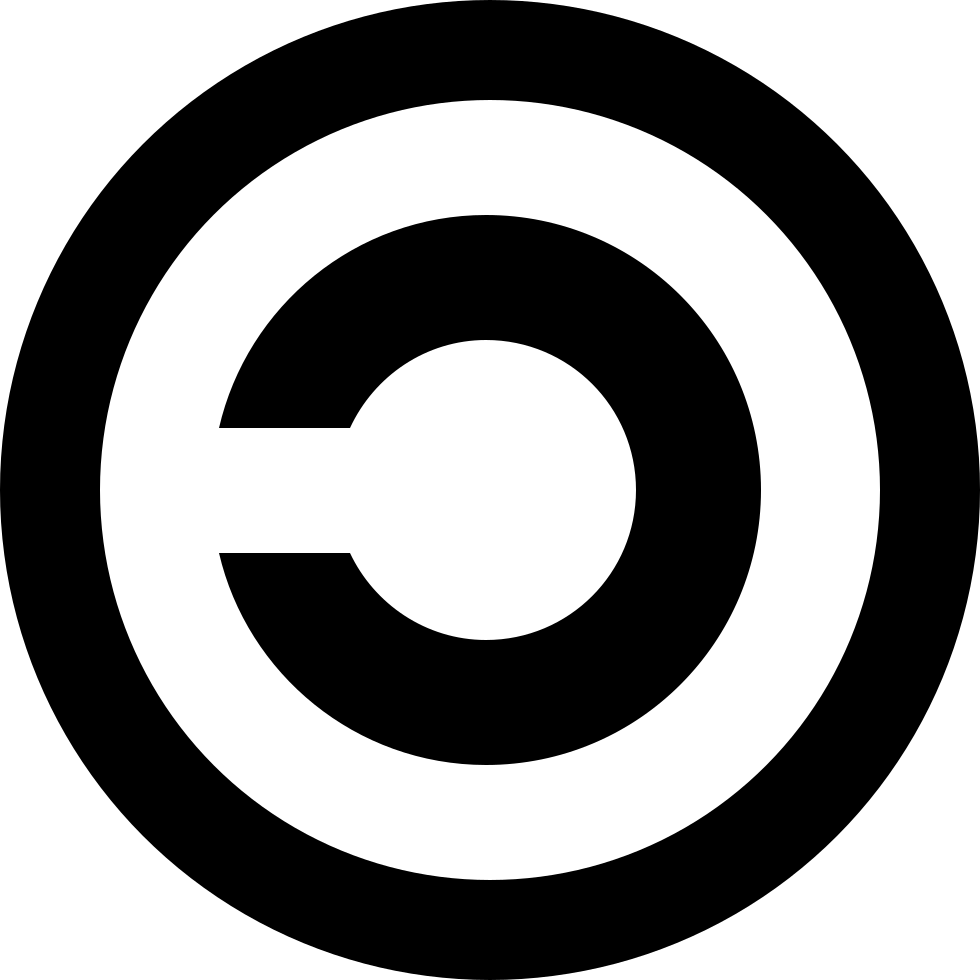
\includegraphics[width=1cm]{Copyleft.svg}
        \else
            
\includegraphics[width=1cm]{Copyleft.eps}
        \fi

Copyright (c) 2011-2012  Laurent Claessens,

Permission is granted to copy, distribute and/or modify this document under the terms of the \href{http://www.gnu.org/licenses/fdl-1.3.html}{GNU Free Documentation License}, Version 1.3 or any later version published by the Free Software Foundation; with no Invariant Sections, no Front-Cover Texts, and no Back-Cover Texts. A copy of the license is included in the section entitled ``GNU Free Documentation License''.

% Ajouter ici l'ISBN. Pour les révisions, mettre un nouvel ISBN et indiquer que c'est une révision.
% Pour l'ISBN:
% Copier tout dans un nouveau répertoire
% Créer une nouvelle branche git
% Coder en dur la date (càd enlever \today)
% Changer la licence vers non modifiable, copiable, et ajouter un lien vers la
%   version modifiable.

% http://www.bnf.fr/fr/professionnels/s_informer_obtenir_isbn/s.qu_est_ce_que_isbn.html

% TODO: écrire le README.txt

\end{center}

\clearpage


}           % Fin d'un ifthenelse sur le CTU

\tableofcontents

\chapter*{Introduction}
\addcontentsline{toc}{chapter}{Introduction}
% This is part of Mes notes de mathématique
% Copyright (c) 2011-2012
%   Laurent Claessens
% See the file fdl-1.3.txt for copying conditions.

%+++++++++++++++++++++++++++++++++++++++++++++++++++++++++++++++++++++++++++++++++++++++++++++++++++++++++++++++++++++++++++
\section{Avertissement}
%+++++++++++++++++++++++++++++++++++++++++++++++++++++++++++++++++++++++++++++++++++++++++++++++++++++++++++++++++++++++++++

Ceci sont des notes «prises au vol» de certains de mes cours pour l'agrégation. Aucune garantie. Merci de me signaler toute faute ou remarque. En particulier je serais content que quelqu'un me donne un avis sur le points suivants :
\begin{enumerate}
    \item
        L'énoncé et la démonstration de la proposition \ref{PropNsLqWb}.
    \item
        Où trouver une preuve de la proposition \ref{PropKZDqTR} sur le supplémentaire topologique ?
    \item
        La preuve du théorème \ref{ThoJsBKir}.
    \item
        La preuve du lemme \ref{LemjXywjH}.
    \item
        La preuve du théorème de Fredholm \ref{ThoagJPZJ}.
    \item
        La preuve du lemme \ref{LemooynkH}.
    \item
        La partie «unicité» du théorème \ref{ThokUUlgU}.
    \item
        La preuve de la proposition \ref{PropRZCKeO}.
    \item
        L'inversion entre la somme et l'intégrale de l'équation \eqref{EqXSgZGw}.
    \item
        Si vous connaissez des exemples ou des contre-exemples intéressants à propos de quoi que ce soit, je suis toujours preneur.
\end{enumerate}

Une version avec ISBN de ce document est en préparation afin qu'il soit acceptable comme livre aux oraux de l'agrégation \ldots j'y travaille et on verra comment les choses vont évoluer.

%+++++++++++++++++++++++++++++++++++++++++++++++++++++++++++++++++++++++++++++++++++++++++++++++++++++++++++++++++++++++++++
\section{Auteurs, contributeurs et remerciements}
%+++++++++++++++++++++++++++++++++++++++++++++++++++++++++++++++++++++++++++++++++++++++++++++++++++++++++++++++++++++++++++

Le principal auteur et metteur en \LaTeX\ de ce document est votre serviteur, Laurent Claessens.

Les personnes qui ont du code \LaTeX\ dans ce document :
\begin{enumerate}
    \item
        Nicolas Richard et Ivik Swan pour les parties des exercices et rappels de calcul différentiel et intégral (Université libre de Bruxelles, 2003-2004) qui leur reviennent.
    \item
        Pierre Bieliavsky pour les énoncés d'analyse numérique (MAT1151 à Louvain la Neuve 2009-2010)
    \item
        Jonathan Di Cosmo pour certaines corrections de MAT1151
\end{enumerate}

Autres sources et remerciements :
\begin{enumerate}
    \item
        Tous les contributeurs du wikipédia francophone (et aussi un peu l'anglophone) doivent être remerciés. J'en ai pompé des quantités astronomiques; des articles utilisés sont cités à divers endroits du texte, mais ce n'est absolument pas exhaustif. Il n'y a à peu près pas un résultat important de ces notes dont je n'aie pas lu la page Wikipédia, et souvent plusieurs pages connexes.
    \item
        Des centaines de profs qui ont mis leurs polys sur internet. Des dizaines d'entre eux (et entre elles) ont des sites dédiés à l'agrégation. Ils sont cités en bibliographie aux endroits où ils sont utilisés. Merci à toutes et à tous d'avoir codé et publié.
    \item
        Le forum usenet de math, en particulier pour la construction des corps fini dans la fil «Vérifier qu'un polynôme est primitif» initié le 20 décembre 2011.
\end{enumerate}

%+++++++++++++++++++++++++++++++++++++++++++++++++++++++++++++++++++++++++++++++++++++++++++++++++++++++++++++++++++++++++++
					\section*{Ces notes sont les vôtres !}
%+++++++++++++++++++++++++++++++++++++++++++++++++++++++++++++++++++++++++++++++++++++++++++++++++++++++++++++++++++++++++


Il y a encore certainement des erreurs, des fautes de frappe et des choses pas claires. Je compte sur vous (oui : toi !) pour me signaler toute imperfection (y compris d'orthographe).

Plus vous signalez de fautes, meilleure sera la qualité du texte, et plus les étudiants de l'année prochaine vous seront reconnaissants.

%Tiens, tant que j'y suis je vous demanderais de penser à la quantité d'argent que vous auriez dû dépenser pour obtenir un texte tel que celui-ci chez un éditeur «classique» qui vous interdirait la photocopie et la redistribution. Maintenant que vous y avez pensé, je vous donnerais bien mon numéro de compte, mais non. J'ai tapé ce texte sur mes heures de travail à l'université; j'ai donc déjà été payé par les contribuables belges et français.

%+++++++++++++++++++++++++++++++++++++++++++++++++++++++++++++++++++++++++++++++++++++++++++++++++++++++++++++++++++++++++++
\section{Contre Moodle, Icampus, Claroline, et autres «plateformes de travail collaboratif»}
%+++++++++++++++++++++++++++++++++++++++++++++++++++++++++++++++++++++++++++++++++++++++++++++++++++++++++++++++++++++++++++

Ces notes ne sont pas destinées à être publiées sur des plateformes telles que Moodle, Icampus ou autres Clarolines. Pourquoi ? parce que la licence FDL l'interdit implicitement en demandant de publier sur des sites \emph{ouverts}.

L'internet est un système décentralisé et ouvert : tout le monde peut s'y connecter, y publier et y lire. C'est pour l'instant la meilleure solution technique inventée par l'humanité pour la diffusion d'information. Des sites comme \href{http://gitorious.org}{gitorious} ou \href{http://wikipedia.org}{wikipedia} sont de \emph{vrais} système de travail collaboratif.

Les plateformes soi-disant collaboratives comme Moodle en sont la négation. L'essentiel de ce qu'apporte Moodle par rapport à un vrai site internet n'est absolument pas la possibilité de partager des information (ça on peut le faire via internet depuis des décennies), mais bien de \emph{restreindre} l'accès à l'information via un système de mot de passe.

Lorsqu'un moine copiste du onzième siècle mettait un manuscrit dans sa bibliothèque, le document était immédiatement consultable par une centaine de moines, et (quitte à faire le déplacement) par des milliers d'érudits. Un document posté sur Moodle touche une dizaine de personnes. Utiliser Moodle pour partager ses documents est donc une régression non pas par rapport à l'internet d'il y a vingt ans, non pas par rapport à l'imprimerie d'il y a cinq siècles, mais bien par rapport aux bibliothèques d'abbayes d'il y a mille ans !

Lorsqu'on parle de science, qu'on veut y apporter un document, une question ou une réponse, un minimum d'honnête intellectuelle, d'éthique du partage de savoir (sans laquelle la science n'existe pas) et peut être aussi de courage, est de parler publiquement. Se cacher derrière un mot de passe et ne permettre l'accès au savoir qu'à ses seuls amis triés sur le volet est une négation de l'esprit scientifique; Moodle est une version dégénérée, une maladie de l'internet.

La faute fondamentale qui fait utiliser Moodle pour partager des documents de mathématique est la perte de notion entre le privé et le public ainsi que la paresse qui consiste à vouloir intégrer tous les outils dans une même interface, voire utiliser les mêmes outils pour effectuer des tâches différentes. Lorsqu'on pose une question de math, c'est essentiellement public; lorsqu'on pose une question d'organisation d'un cours, c'est privé. Ce sont deux activités totalement différentes qui nécessitent deux types d'outils différents. Dans le premier cas, l'outil adapté est internet, dans le deuxième cas, l'outil adapté est Moodle. Vouloir utiliser la même interface pour les deux est n'avoir fondamentalement pas compris le sens de l'internet et son utilité en tant que «outil de l'information».

{\tiny Cela dit c'est pratique pour discuter des horaires des cours ou s'échanger des informations pratiques qui n'ont pas à être publiques.}

%+++++++++++++++++++++++++++++++++++++++++++++++++++++++++++++++++++++++++++++++++++++++++++++++++++++++++++++++++++++++++++
\section{Instructions pour les examens et interrogations}
%+++++++++++++++++++++++++++++++++++++++++++++++++++++++++++++++++++++++++++++++++++++++++++++++++++++++++++++++++++++++++++

Ceci sont des conseils généraux que nous vous conseillons de suivre dans toutes les matières.
\begin{description}
    \item[numéroter] Numérotez clairement toutes les questions. Si votre réponse prend plus d'une page, écrivez «suite au verso», «suite à l'intercalaire \( n\)» etc. À l'endroit où la réponse continue, écrivez «question \( n\), suite».

    \item[vérifiez] Certaines erreurs sont faciles à détecter. Par exemple
        \begin{enumerate}
            \item
                les aires et volumes sont positifs;
            \item
                une intégrale \emph{définie} qui contient «\( dx\)» ne peut pas contenir de \( x\) dans la réponse;

            \item
                en physique et en chimie, les unités doivent être cohérentes : si la réponse est une énergie, vous devez avoir des joules (\unit{\square\metre\kilo\gram\per\square\second}).

        \end{enumerate}
    \item[votre nom] Écrivez votre nom et votre numéro de carte d'étudiant.

    \item[les faciles d'abord] Lisez d'abord toutes les questions avant de répondre. Commencez par les questions faciles.

    \item[justifier] Justifiez vos réponses. N'hésitez pas à écrire des phrases complètes : sujet, verbe, complément. N'abusez pas des symboles dont vous ignorez la signification :
        \begin{enumerate}
            \item
                «\( \Leftrightarrow\)» signifie «si et seulement si», et non «la suite de mon calcul»;
            \item

                «\( \nexists\)» signifie «il n'existe pas», et non «n'existe pas» ou «n'est pas défini».
        \end{enumerate}

    \item[ne pas passer en force] Si vous savez que votre réponse est fausse, mais vous ne savez pas la corriger, écrivez sur votre feuille «cette réponse est fausse pour telle raison, mais je ne sais pas comment corriger». Ne comptez pas sur une inattention du correcteur. En science, affirmer un fait que vous savez être faux s'appelle de la falsification; c'est déontologiquement inacceptable. De la même façon, si vous copiez sur votre voisin\footnote{Indépendamment que c'est sans doute interdit par le règlement; vérifiez avant.}, vous êtes priés de le citer : on ne s'approprie pas le travail d'autrui.

    \item[approximations numériques] Lorsque vous voulez écrire une approximation numérique, réfléchissez au sens de ce que vous allez écrire. En mathématique, ça n'a presque jamais de sens d'écrire une approximation parce que vous ne savez pas dans quel contexte votre calcul pourra être utilisé. Si vous laissez deux décimales à \( \pi\) pour calculer le volume d'eau dans votre piscine gonflable, ça fera l'affaire; si c'est pour calculer la masse du Higgs ou pour mettre un satellite autour de Mars, vous perdez plusieurs millions d'euros.

        En sciences naturelles (physique, chimie ou autres), vous pouvez donner des approximations numériques de façon circonstanciée. Demandez à votre prof de labo.

    \item[orthographe] Sans être obligatoire, ça ne fait jamais de mal. Surtout si le français est votre langue maternelle.
    \item[santé] Mangez des fruits et des légumes de saisons. Choisissez des producteurs locaux qui n'utilisent pas d'engrais synthétisés à base de pétrole. De toutes façons \href{http://www.energybulletin.net/node/51306}{vous n'avez pas le choix}.

\end{description}

%+++++++++++++++++++++++++++++++++++++++++++++++++++++++++++++++++++++++++++++++++++++++++++++++++++++++++++++++++++++++++++
\section{Propagande : utilisez un ordinateur !}
%+++++++++++++++++++++++++++++++++++++++++++++++++++++++++++++++++++++++++++++++++++++++++++++++++++++++++++++++++++++++++++

Si vous faites des exercices supplémentaires et que vous voulez des corrections, n'oubliez pas que vous avez un ordinateur à disposition. De nos jours, les ordinateurs sont capables de calculer à peu près tout ce qui se trouve dans vos cours de math\footnote{Avec une notable exception pour les limites à deux variables.}.

D'ailleurs, je te rappelle que nous sommes est déjà largement dans le vingt et unième siècle et que tu te destines à une carrière professionnelle dans laquelle tu auras des calculs à faire; si tu n'es pas encore capable d'utiliser un ordinateur pour faire ces calculs, il est temps de combler cette lacune.

%---------------------------------------------------------------------------------------------------------------------------
\subsection{Lancez-vous dans Sage}
%---------------------------------------------------------------------------------------------------------------------------

Le logiciel que je vous propose est \href{http://www.sagemath.org}{Sage}. Pour l'utiliser, il n'est même pas nécessaire de l'installer sur votre ordinateur~: il tourne en ligne, directement dans votre navigateur.

\begin{enumerate}

	\item
		Aller sur \href{http://www.sagenb.org}{http://www.sagenb.org}
	\item
		Créer un compte
	\item
		Créer des feuilles de calcul et amusez-vous !!

\end{enumerate}

Il y a beaucoup de \href{http://lmgtfy.com/?q=sage+documentation}{documentation} sur le \href{http://www.sagemath.org}{site officiel}\footnote{\href{http://www.sagemath.org}{http://www.sagemath.org}}.

Si vous comptez utiliser régulièrement ce logiciel, je vous recommande \emph{chaudement} de \href{http://mirror.switch.ch/mirror/sagemath/index.html}{l'installer} sur votre ordinateur. Ce logiciel étant distribué sous licence GPL, vous ne devez ni payer ni vous procurer de codes.

%---------------------------------------------------------------------------------------------------------------------------
\subsection{Exemples de ce que Sage peut faire pour vous}
%---------------------------------------------------------------------------------------------------------------------------

Voici une liste absolument pas exhaustive de ce que Sage peut faire pour vous, avec des exemples. 
\begin{enumerate}

	\item
		Calculer des limites de fonctions, voir l'exercice \ref{exoINGE11140028},

	\item
		D'autres limites et tracer des fonctions, voir l'exercice \ref{exoINGE11140031}.
	\item
		Calculer des dérivées, voir exercice \ref{exo0013}.
	\item
		Calculer des dérivées partielles de fonctions à plusieurs variables, voir exercice \ref{exoFoncDeuxVar0002}.
	\item
		Calculer des primitives, voir certains exercices \ref{exo0017}
	\item

		Résoudre des systèmes d'équations linéaires. Lire \href{http://www.sagemath.org/doc/constructions/linear_algebra.html#solving-systems-of-linear-equations}{la documentation} est ce qui fait la différence entre l'être humain et le non scientifique. Voir les exercices  \ref{exoINGE1121La0016} et \ref{exoINGE1121La0010}.

	\item
		Tout savoir d'une forme quadratique, voir exercice \ref{exoINGE1121La0018}.
	\item
		Calculer la matrice Hessienne de fonctions à deux variables, déterminer les points critiques, déterminer le genre de la matrice Hessienne aux points critiques et écrire extrema de la fonctions (sous réserve d'être capable de résoudre certaines équations), voir les exercices \ref{exoFoncDeuxVar0029} et \ref{exoFoncDeuxVar0028}.
	\item
		Lorsqu'il y a une infinité de solutions, Sage vous l'indique avec des paramètres (ne fonctionne hélas pas avec les fonctions trigonométriques), voir l'exercice \ref{exoDerrivePartielle-0007}.


	\item
		Calculer des dérivées symboliquement, voir exercice \ref{exoDerive-0002}.
	\item
		Calculer des approximations numériques comme dans l'exercice \ref{exoOutilsMath-0028}.
    \item
        Calculer dans un corps de polynômes modulo comme \( \eF_p[X]/P\) où \( P\) est un polynôme à coefficients dans \( \eF_p\). Voir l'exemple \ref{ExemWUdrcs}.
	\item
        Tracer des courbes en trois dimensions, voir exemple \ref{ExempleTroisDxxyy}. Notez que pour cela vous devez installer aussi le logiciel Jmol. Pour Ubuntu\footnote{Pour les autres, je ne sais pas, mais je laisserai jouer l' adage «Windows c'est facile». Quant aux utilisateurs d'OS «alternatifs» comme Hurd ou BSD ben heu \ldots} c'est dans le paquet \info{icedtea6-plugin}.
\end{enumerate}

Sage peut toutefois vous induire en erreur si vous n'y prenez pas garde parce qu'il sait des choses en mathématique que vous ne savez pas. Par conséquent il peut parfois vous donner des réponses (mathématiquement exactes) auxquelles vous ne vous attendez pas. Voir page \ref{PgpXBuBh}.

%+++++++++++++++++++++++++++++++++++++++++++++++++++++++++++++++++++++++++++++++++++++++++++++++++++++++++++++++++++++++++++
%\section{Propagande : n'utilisez pas votre calculatrice}
%+++++++++++++++++++++++++++++++++++++++++++++++++++++++++++++++++++++++++++++++++++++++++++++++++++++++++++++++++++++++++++

%D'abord, l'expérience montre que la majorité des fois qu'un étudiant sort sa calculatrice, c'est pour faire un calcul inutile, et le plus souvent la calculatrice fournit un résultat faux. Étant en 2012, vous ne devriez pas vous contenter de vos calculatrices qui coûtent un os, qui n'ont pas de puissance de calcul, qui ont une définition d'écran ridicule et en noir et blanc. Remarquez que votre GSM (et a forciori vos minis trucs qui se connectent a internet) sont considérablement plus puissants que ces vieilleries; ils ont un meilleur écran.


\ifthenelse{\value{ThisIsCTU}=1}{
    \newcounter{bidon}
    \setcounter{bidon}{\value{page}}
    \mainmatter
    \stepcounter{bidon}
    \setcounter{page}{\value{bidon}}
}{}


%% ATTENTION : (note de Laurent pour Laurent qui n'intéresse pas tellement les autres)
%%
% Ce cours est inclus dans «Mes notes de mathématique»[1].
% La seule partie qui y est hard-codée est la suite des inputs pour les chapitres.
% Si on modifie ici, il faut aussi modifier là-bas.
% Ne pas oublier de copier les input des appendices

% [1] http://student.ulb.ac.be/~lclaesse/mes_notes.pdf


\chapter{Topologie des espaces vectoriels normés}      \label{ChapEspVectNorm}

Ce chapitre va traiter d'espaces vectoriels muni d'une notion de «taille» d'un vecteur. Le principal exemple qu'il faut avoir en tête tout au long du chapitre est $\eR^m$ muni de la norme euclidienne; nous entreverrons dans la section \ref{normes_equiv} pourquoi l'intuition sur cet exemple particulier fonctionne tellement bien. Il faut cependant garder à l'esprit que d'autres exemples existent : nous verrons le cas de l'espace des applications linéaires au chapitre \ref{Chap_appl_lin}.

La définition d'une norme est donnée dans la section \ref{Sect_definition}. Les sections suivantes, \ref{Sect_boules} et \ref{Sect_topologie}, présentent la topologie des espaces vectoriels de dimension finie. Cette topologie, comme vous verrez, découle immédiatement de la norme introduite. On parle alors de topologie \emph{induite par la norme}. Dans la section \ref{Sect_suites} nous  donnons la définition de suite convergente de vecteurs et dans la section \ref{Sect_fonctions} la définition de fonction continue. Enfin, la section \ref{sec_prod} parle de normes et de la topologie des espaces vectoriels qui sont le produit de deux (ou plus) espaces vectoriels de dimension finie.

Tout le matériel présenté dans ce chapitre est sujet d'examen à l'exclusion de

\begin{itemize}
\item la partie de la section \ref{Sect_fonctions} qui suit la définition \ref{DefContDansEVN};
\item les démonstrations de la section \ref{sec_prod};
\item la sous-section \ref{SubSecPOlynomesCE};
\end{itemize}

%+++++++++++++++++++++++++++++++++++++++++++++++++++++++++++++++++++++++++++++++++++++++++++++++++++++++++++++++++++++++++++
\section{Introduction}
%+++++++++++++++++++++++++++++++++++++++++++++++++++++++++++++++++++++++++++++++++++++++++++++++++++++++++++++++++++++++++++

La valeur absolue est essentielle pour introduire les notions de limite et de continuité pour les fonctions d'une variable (voir appendice \ref{AppendiceAnalyseR} pour un rappel). En fait nous disons que la fonction $f\colon \eR\to \eR$ est continue au point $a$ lorsque pour tout $\varepsilon$, il existe un $\delta$ tel que
\begin{equation}
	| x-a |\leq\delta \Rightarrow | f(x)-f(a) |\leq \varepsilon.
\end{equation}
La quantité $| x-a |$ donne la «distance» entre $x$ et $a$; la définition de la continuité signifie que pour tout $\varepsilon$, il existe un $\delta$ tel que si $a$ et $x$ sont au plus à la distance $\delta$ l'un de l'autre, alors $f(x)$ et $f(a)$ ne seront éloigné au plus d'une distance $\varepsilon$.

La valeur absolue, dans $\eR$, nous sert donc à mesurer des distances entre les nombres. Les principales propriétés de la valeur absolue sont :
\begin{enumerate}

	\item
		$| x |=0$ implique $x=0$,
	\item
		$| \lambda x |=| \lambda | |x |$,
	\item
		$| x+y |\leq | x |+| y |$

\end{enumerate}
pour tout $x,y\in\eR$ et $\lambda\in\eR$.

Afin de donner une notion de limite pour les fonctions de plusieurs variables, nous devons trouver un moyen de définir les notion de <<taille>> d'un vecteur et de distance entre deux points de $\eR^n$, avec $n>1$. La notion de <<taille>> doit satisfaire propriétés analogues à celles de la valeur absolue. 

La premier notion de <<taille>> pour un vecteur de $\eR^2$ que nous vient à l'esprit est la longueur du segment entre l'origine et l'extrémité libre du vecteur. Cela peut être calculée à l'aide du théorème de Pythagore : 
\begin{equation}
  \textrm{taille de } (a,b) = \sqrt{a^2+b^2}.
\end{equation}
Nous pouvons introduire une la notion de distance entre les éléments de $\eR^2$ de façon similaire :
\begin{equation}
	d\big((a_x,a_y),(b_x,b_y)\big)=\sqrt{  (a_x-b_x)^2+(a_y-b_y)^2  }.
\end{equation}
Cette définition a l'air raisonnable; est-elle mathématiquement correcte ? Peut-elle jouer le rôle de la valeur absolue dans $\eR^2$ ? Est-elle la seule définitions possibles de <<taille>> et distance en $\eR^2$ ?  


%+++++++++++++++++++++++++++++++++++++++++++++++++++++++++++++++++++++++++++++++++++++++++++++++++++++++++++++++++++++++++++
\section{Normes et distances}\label{Sect_definition}
%+++++++++++++++++++++++++++++++++++++++++++++++++++++++++++++++++++++++++++++++++++++++++++++++++++++++++++++++++++++++++++

Nous voulons formaliser les notions de «taille» et de distance dans $\eR^n$, et plus généralement dans un espace vectoriel $V$ de dimension finie. Pour cela nous nous inspirons des propriétés de la valeur absolue.
\begin{definition}		\label{DefNorme}
	Soit $V$ un espace vectoriel réel. Une \defe{norme}{norme!définition} est une application $N\colon V\to \eR^+$ vérifiant les axiomes 
	\begin{enumerate}

		\item
			$N(0_V)=0$, et $N(x)=0$ implique $x=0_V$;
		\item\label{ItemDefNormeii}
			$N(\lambda x)=| \lambda |N(x)$ pour tout $\lambda\in\eR$ et $x\in V$;
		\item\label{ItemDefNormeiii}
			$N(x+y)\leq N(x)+N(y)$ pour tout $x,y\in V$. Cette propriété est appelée \defe{inégalité triangulaire}{inégalité triangulaire}.
	\end{enumerate}
	Ici et dans la suite, $0_V$ désigne l'élément zéro de l'espace $V$.
\end{definition}
En prenant $\lambda=-1$ dans la propriété \ref{ItemDefNormeii}, nous trouvons immédiatement que $N(-x)=N(x)$.

\begin{proposition}		\label{PropNmNNm}
	Toute norme $N$ sur l'espace vectoriel $V$ vérifie l'inégalité
	\begin{equation}
		\big| N(x)-N(y) \big|\leq N(x-y)
	\end{equation}
	pour tout $x,y\in V$.
\end{proposition}
	
\begin{proof}
	Nous avons, en utilisant le point \ref{ItemDefNormeiii} de la définition \ref{DefNorme},
	\begin{subequations}
		\begin{align}
			N(x)&=N(x-y+y)\leq N(x-y)+N(y),	\label{subEqNNNxxyyya}\\
			N(y)&=N(y-x+x)\leq N(y-x)+N(x).	\label{subEqNNNxxyyyb}
		\end{align}
	\end{subequations}
	Supposons d'abord que $N(x)\geq N(y)$. Dans ce cas, en utilisant \eqref{subEqNNNxxyyya},
	\begin{equation}
		\big| N(x)-N(y) \big|=N(x)-N(y)\leq N(x-y)+N(y)-N(y)=N(x-y).
	\end{equation}
	Si par contre $N(x)\leq N(y)$, alors nous utilisons \eqref{subEqNNNxxyyyb} et nous trouvons
	\begin{equation}
		\big| N(x)-N(y) \big|=N(y)-N(x)\leq N(y-x)+N(x)-N(x)=N(y-x).
	\end{equation}
	Dans les deux cas, nous avons retrouvé l'inégalité annoncée.
\end{proof}
Cette proposition signifie aussi que
\begin{equation}	\label{EqNleqNNleqNvqlqbs}
	-N(x-y)\leq N(x)-N(y)\leq N(x-y).
\end{equation}

Afin de suivre une notation proche de celle de la valeur absolue, à partir de maintenant, la norme d'un vecteur $v$ sera notée $\| v\|$ au lieu de $N(v)$.
\begin{definition}		\label{DefEVNetDistance}
	Un espace vectoriel $V$ muni d'une norme est une \defe{espace vectoriel normé}{normé!espace vectoriel}, et on écrit $(V,\| . \|)$. La \defe{distance induite}{distance (d'une norme)} par la norme entre les points $a$ et $b$ de $V$ est le nombre $d(a,b)=\| a-b \|$.

	Si $A$ est une partie de $V$ et si $x\in V$, nous disons que la \defe{distance}{distance!point et ensemble} entre $A$ et $x$ est le nombre
	\begin{equation}		\label{EqdefDistaA}
		d(x,A)=\inf_{a\in A}d(x,a).
	\end{equation}
\end{definition}
%The result is on the figure \ref{LabelFigDistanceEnsemble}
\newcommand{\CaptionFigDistanceEnsemble}{La distance entre $x$ et $A$ est donnée par la distance entre $x$ et $p$. Les distances entre $x$ et les autres points de $A$ sont plus grandes que $d(x,p)$.}
\input{Fig_DistanceEnsemble.pstricks}

Il est possible de définir de nombreuses normes sur $\eR^n$. Citons en quelque unes. Les normes $\| . \|_{L^p}$ ($p\in\eN$) sont définies de la façon suivante :
\begin{equation}		\label{EqDeformeLp}
	\| x \|_{L^p}=\Big( \sum_{i=1}^n| x_i |^p\Big)^{1/p},
\end{equation}
pour tout $x=(x_1,\ldots,x_n)\in\eR^n$. Parmi ces normes, celles qui seront le plus souvent utilisées dans ces notes sont
\begin{equation}
	\begin{aligned}[]
		\| x \|_{L^1}&=\sum_{i=1}^n| x_i |,\\
		\| x \|_{L^2}&=\Big( \sum_{i=1}^n| x_i |^2 \Big)^{1/2}.
	\end{aligned}
\end{equation}
La norme $L^2$ est la \defe{norme euclidienne}{norme!euclidienne}. Nous définissons également la \defe{norme supremum}{norme!supremum} par
\begin{equation}
	\| x \|_{\infty}=\sup_{1\leq i\leq n}| x_i |.
\end{equation}
Nous admettons sans démonstration que les fonctions $\| . \|_{L^p}\colon \eR^n\to \eR^+$ sont bien des normes.

\newcommand{\CaptionFigDistanceEuclide}{La \emph{norme} euclidienne induit la \emph{distance} euclidienne. D'où son nom. Le point $C$ est construit aux coordonnées $(A_x,B_y)$.}
\input{Fig_DistanceEuclide.pstricks}

Soient $A=(A_x,A_y)$ et $B=(B_x,B_y)$ deux éléments de $\eR^2$. La distance\footnote{Ne pas confondre «distance» et «norme».} euclidienne entre $A$ et $B$ est donnée par $\| A-B \|_2$. En effet, sur la figure \ref{LabelFigDistanceEuclide}, la distance entre les points $A$ et $B$ est donnée par
\begin{equation}
	| AB |^2=| AC |^2+| CB |^2=| A_x-B_x |^2+| A_y-B_y |^2,
\end{equation}
par conséquent,
\begin{equation}
	| AB |=\sqrt{| A_x-B_x |^2+| A_y-B_y |^2}=\| A-B \|_2.
\end{equation}

\begin{remark}
	Si $A$, $B$ et $C$ sont trois points dans le plan $\eR^2$, alors l'inégalité triangulaire $| AB |\leq| AC |+| CB |$ est précisément la propriété \ref{ItemDefNormeiii} de la norme (définition \ref{DefNorme}). En effet l'inégalité triangulaire s'exprime de la façon suivante en terme de la norme $\| . \|_2$ :
	\begin{equation}	\label{EqNDeuxAmBNNdd}
		\| A-B \|_2\leq \| A-C \|_2+\| C-B \|_2.
	\end{equation}
	En notant $u=A-C$ et $v=C-B$, l'équation \eqref{EqNDeuxAmBNNdd} devient exactement la propriété de définition de la norme :
	\begin{equation}
		\| u+v \|_2\leq \| u \|_2+\| v \|_2.
	\end{equation}
	Ceci explique pourquoi cette propriété des norme est appelée «inégalité triangulaire».
\end{remark}

Les distances que nous avons vues jusqu'à présent sont des distances définies à partir d'une norme. La définition suivante donne une notion générale de distance sur un espace vectoriel \( V\).

\begin{definition}
    Soit \( V\) un espace vectoriel. Une \defe{distance}{distance} sur \( V\) est une application \( d\colon V\times V\to \eR\) telle que
    \begin{enumerate}
        \item
            \( d(x,y)\geq 0\) pour tout \( x,y\in V\);
        \item
            \( d(x,y)=0\) si et seulement si \( x=y\);
        \item
            \( d(x,y)=d(y,x)\) pour tout \( x,y\in V\);
        \item
            \( d(x,y)\leq d(x,z)+d(z,y)\) pour tout \( x,y,z\in V\).
    \end{enumerate}
    La dernière condition est l'inégalité triangulaire. Le nombre \( d(x,y)\) est la \emph{distance} entre \( x\) et \( y\).
\end{definition}
Toute distance définit une norme en posant \( \| v \|=d(v,0)\).

%+++++++++++++++++++++++++++++++++++++++++++++++++++++++++++++++++++++++++++++++++++++++++++++++++++++++++++++++++++++++++++
\section{Boules et sphères}\label{Sect_boules}
%+++++++++++++++++++++++++++++++++++++++++++++++++++++++++++++++++++++++++++++++++++++++++++++++++++++++++++++++++++++++++++

\begin{definition}
	Soit $(V,\| . \|)$, un espace vectoriel normé, $a\in V$ et $r>0$. Nous allons abondamment nous servir des ensembles suivants :
	\begin{enumerate}

		\item
			la \defe{boule ouverte}{boule!ouverte} $B(a,r)=\{ x\in V\tq \| x-a \|<r \}$;
		\item
			la \defe{boule fermée}{boule!fermée} $\bar B(a,r)=\{ x\in V\tq \| x-a \|\leq r \}$;
		\item
			la \defe{sphère}{sphère} $S(a,r)=\{ x\in V\tq \| x-a \|=r \}$.

	\end{enumerate}
\end{definition}
Les différences entre ces trois ensembles sont très importantes. D'abord, les \emph{boules} sont pleines tandis que la \emph{sphère} est creuse. En comparant à une pomme, la boule ouverte serait la pomme «sans la peau», la boule fermée serait «avec la peau» tandis que la sphère serait seulement la peau. Nous avons
\begin{equation}
	\bar B(a,r)=B(a,r)\cup S(a,r).
\end{equation}

\begin{definition}
	Une partie $A$ de $V$ est dite \defe{bornée}{borné!partie de $V$} si il existe un réel $R$ tel que $A\subset B(0_V,R)$.
\end{definition}
Une partie est donc bornée si elle est contenue dans une boule de rayon fini.

\begin{example}
	Dans $\eR$, les boules sont  les intervalles ouverts et fermés tandis que la sphère est donnée par les points extrêmes des intervalles :
	\begin{equation}
		\begin{aligned}[]
			B(a,r)&=\mathopen] a-r , a+r \mathclose[,\\
			\bar B(a,r)&=\mathopen[ a-r , a+b \mathclose],\\
			S(a,r)&=\{ a-r,a+r \}.
		\end{aligned}
	\end{equation}
\end{example}

\begin{example}
	Si nous considérons $\eR^2$, la situation est plus riche parce que nous avons plus de normes. Essayons de voir les sphères de centre $(0,0)\in\eR^2$ et de rayon $r$ pour les normes $\| . \|_1$, $\| . \|_2$ et $\| . \|_{\infty}$.

	Pour la norme $\| . \|_1$, la sphère de rayon $r$ est donnée par l'équation
	\begin{equation}
		| x |+| y |=r.
	\end{equation}
	Pour la norme $\| . \|_2$, l'équation de la sphère de rayon $r$ est
	\begin{equation}
		\sqrt{x^2+y^2}=r,
	\end{equation}
	et pour la norme supremum, la sphère de rayon $r$ a pour équation
	\begin{equation}
		\max\{ | x |,| y | \}=r.
	\end{equation}
	Elles sont dessinées sur la figure \ref{LabelFigLesSpheres}
\newcommand{\CaptionFigLesSpheres}{Les sphères de rayon $1$ pour les trois normes classiques.}
\input{Fig_LesSpheres.pstricks}
\end{example}

\newcommand{\CaptionFigBoulePtLoin}{Le point $P$ est un peu plus loin que $x$, en suivant la même droite.}
\input{Fig_BoulePtLoin.pstricks}

\begin{proposition}		\label{PropBoitPtLoin}
	Soient $V$ un espace vectoriel normé, $a$ dans $V$ et $x$ tel que $d(a,x)=r$, c'est à dire $x\in S(a,r)$. Dans ce cas, toute boule centrée en $x$ contient un point $P$ tel que $d(P,a)>r$ et un point $Q$ tel que $d(Q,a)<r$.
\end{proposition}

\begin{proof}
	Soit une boule de rayon $\delta$ autour de $x$. Le but est de trouver un point $P$ tel que $d(P,a)>r$ et $d(P,x)<\delta$. Pour cela, nous prenons $P$ sur la même droite que $x$ (en partant de $a$), mais juste «un peu plus loin» (voir figure \ref{LabelFigBoulePtLoin}). Plus précisément, nous considérons le point
	\begin{equation}
		P=x+\frac{ v }{ N }
	\end{equation}
	où $v=x-a$ et $N$ est suffisamment grand pour que $d(x,P)$ soit plus petit que $\delta$. Cela est toujours possible parce que
	\begin{equation}
		d(P,x)=\| P-x \|=\frac{ \| v \| }{ N }
	\end{equation}
	peut être rendu aussi petit que l'on veut par un choix approprié de $N$. Montrons maintenant que $d(a,P)>d(a,x)$ :
	\begin{equation}
		\begin{aligned}[]
			d(a,P)&=\| a-x-\frac{ v }{ N }\| \\
			&=\| a-x+\frac{ a }{ N }-\frac{ x }{ N } \|\\
			&=\| \big( 1+\frac{1}{ N }(a-x) \big) \|\\
			&>\| a-x \|=d(a,x).
		\end{aligned}
	\end{equation}
	Nous laissons en exercice le soin de trouver un point $Q$ tel que $d(Q,a)<r$ et $d(Q,x)<\delta$.
\end{proof}

%+++++++++++++++++++++++++++++++++++++++++++++++++++++++++++++++++++++++++++++++++++++++++++++++++++++++++++++++++++++++++++
\section{Topologie}\label{Sect_topologie}
%+++++++++++++++++++++++++++++++++++++++++++++++++++++++++++++++++++++++++++++++++++++++++++++++++++++++++++++++++++++++++++

%---------------------------------------------------------------------------------------------------------------------------
\subsection{Ouverts, fermés, intérieur et adhérence}
%---------------------------------------------------------------------------------------------------------------------------

\begin{definition}
	Soit $(V,\| . \|)$ un espace vectoriel normé et $A$, une partie de $V$. Un point $a$ est dit \defe{intérieur}{intérieur!point} à $A$ si il existe une boule ouverte centrée en $a$ et contenue dans $A$.

	On appelle \defe{l'intérieur}{intérieur!d'un ensemble} de $A$ l'ensemble des points qui sont intérieurs à $A$. Nous notons $\Int(A)$ l'intérieur de $A$.
\end{definition}
Notons que $\Int(A)\subset A$ parce que si $a\in\Int(A)$, nous avons $B(a,r)\subset A$ pour un certain $r$ et en particulier $a\in A$.

\begin{example}
	Trouver l'intérieur d'un intervalle dans $\eR$ consiste à «ouvrir là où c'est fermé». 
	\begin{enumerate}

		\item
			$\Int\big(\mathopen[ 0 , 1 [\big)=\mathopen] 0 , 1 \mathclose[$. 
			
			Prouvons d'abord que $\mathopen] 0,1  \mathclose[\subset\Int(\mathopen[ 0 , 1 [)$. Si $a\in\mathopen] 0 , 1 \mathclose[$, alors $a$ est strictement supérieur à $0$ et strictement inférieur à $1$. Dans ce cas, la boule de centre $a$ et de rayon $\frac{ \min\{ a,1-a \} }{ 2 }$ est contenue dans $\mathopen] 0 , 1 \mathclose[$ (voir figure \ref{LabelFigIntervalle}). Cela prouve que $a$ est dans l'intérieur de $\mathopen[ 0 , 1 [$.

\newcommand{\CaptionFigIntervalle}{Trouver le rayon d'une boule autour de $a$. Une boule qui serait centrée en $a$ avec un rayon strictement plus petit à la fois de $a$ et de $1-a$ est entièrement contenue dans le segment $\mathopen] 0 , 1 \mathclose[$.}
\input{Fig_Intervalle.pstricks}

			Prouvons maintenant que $\Int\big( \mathopen[ 0 , 1 [ \big)\subset\mathopen] 0 , 1 \mathclose[$. Vu que l'intérieur d'un ensemble est inclus à l'ensemble, nous savons déjà que $\Int\big( \mathopen[ 0 , 1 [ \big)\subset\mathopen[ 0 , 1 [$. Nous devons donc seulement montrer que $0$ n'est pas dans l'intérieur de $\mathopen[ 0 , 1 [$. C'est le cas parce que toute boule du type $B(0,r)$ contient le point $-r/2$ qui n'est pas dans $\mathopen[ 0 , 1 [$.

		\item
			$\Int\Big( \mathopen[ 0 , \infty [ \Big)=\mathopen] 0 , \infty \mathclose[$.
		\item
			$\Int\big( \mathopen] 2 , 3 \mathclose[ \big)=\mathopen] 2 , 3 \mathclose[$.

	\end{enumerate}
	
\end{example}

\begin{example}			\label{ExempleIntBoules}
	Les intérieurs des boules et sphères sont importantes à savoir.
	\begin{enumerate}
		\item 
			$\Int\big( B(a,r) \big)=B(a,r)$. Si $x\in B(a,r)$, nous avons $d(a,x)<r$. Alors la boule $B\big(x,r-d(x,a)\big)$ est incluse à $B(a,r)$, et donc $x$ est dans l'intérieur de $B(a,r)$. Conseil : faire un dessin.
		\item
			$\Int\big( \bar B(a,r) \big)=B(a,r)$. Par le point précédent, la boule $B(a,r)$ est certainement dans l'intérieur de la boule fermée. Il reste à montrer que les points de $\bar B(a,r)$ qui ne sont pas dans $B(a,r)$ ne sont pas dans l'intérieur. Ces points sont ceux dont la distance à $a$ est \emph{égale} à $r$. Le résultat découle alors de la proposition \ref{PropBoitPtLoin}.
			
		\item
			$\Int\big( S(a,r) \big)=\emptyset$. Si $x\in S(a,r)$, toute boule centrée en $a$ contient des points qui ne sont pas à distance $r$ de $a$.
			
			Notez que la sphère est un exemple d'ensemble non vide mais d'intérieur vide.
	\end{enumerate}
\end{example}


\begin{definition}
	Une partie $A$ de l'espace vectoriel normé $(V,\| . \|)$ est dite \defe{ouverte}{ouvert} si chacun de ses points est intérieur. La partie $A$ est donc ouverte si $A\subset\Int(A)$. Par convention, nous disons que l'ensemble vide $\emptyset$ est ouvert.

	Une partie est dite \defe{fermée}{fermé} si son complémentaire est ouvert. La partie $A$ est donc fermée si $V\setminus A$ est ouverte.
\end{definition}

Remarque : un ensemble $A$ est ouvert si et seulement si $\Int(A)=A$.

\begin{definition}
	Une partie $A$ de l'espace vectoriel normé $V$ est dite \defe{compacte}{compact} si elle est fermée et bornée.
\end{definition}

Nous verrons tout au long de ce cours que les ensembles compacts, et les fonctions définies sur ces ensembles ont de nombreuses propriétés agraables.

\begin{example}		\label{ExempleFermeIntevrR}
	En ce qui concerne les intervalles de $\eR$,
	\begin{itemize}
		\item $\mathopen] 1 , 2 \mathclose[$ est ouvert;
		\item $\mathopen[ 3,  4 \mathclose]$ est fermé;
		\item $\mathopen[ 5 , 6 [$ n'est ni ouvert ni fermé;
	\end{itemize}
	Les intervalles fermés de $\eR$ sont toujours compacts.
\end{example}

\begin{proposition}		\label{PropTopologieAx}
	Soit $V$ un espace vectoriel normé.
	\begin{enumerate}
		\item
			L'ensemble $V$ lui-même et le vide sont à la fois fermées et ouvertes.
		\item
			Toute union d'ouverts est ouverte.
		\item
			Toute intersection \emph{finie} d'ouverts est ouverte.
		\item		\label{ItemPropTopologieAxiv}
			Le vide et $V$ sont les seules parties de $V$ à être à la fois fermées et ouvertes.
	\end{enumerate}
\end{proposition}

\begin{proof}
	L'ingrédient principal de cette démonstration est que si $a$ est un point d'un ouvert $\mO$, alors il existe une boule autour de $a$ contenue dans $\mO$ parce que $a$ doit être dans l'intérieur de $\mO$.
	\begin{enumerate}

		\item
			Nous avons déjà dit que, par définition, l'ensemble vide est ouvert. Cela implique que $V$ lui-même est fermé (parce que son complémentaire est le vide). De plus, $V$ est ouvert parce que toutes les boules sont inclues à $V$. Le vide est alors fermé (parce que son complémentaire est $V$).
		\item
			Soit une famille $(\mO_i)_{i\in I}$ d'ouverts\footnote{L'ensemble $I$ avec lequel nous «numérotons» les ouverts $\mO_i$ est \emph{quelconque}, c'est à dire qu'il peut être $\eN$, $\eR$, $\eR^n$ ou n'importe quel autre ensemble, fini ou infini.}, et l'union
			\begin{equation}
				\mO=\bigcup_{i\in I}\mO_i.
			\end{equation}
			Soit maintenant $a\in\mO$. Nous devons prouver qu'il existe une boule centrée en $a$ entièrement contenue dans $\mO$. Étant donné que $a\in\mO$, il existe $i\in I$ tel que $a\in\mO_i$ (c'est à dire que $a$ est au moins dans un des $\mO_i$). Par hypothèse l'ensemble $\mO_i$ est ouvert et donc tous ses points (en particulier $a$) sont intérieurs; il existe donc une boule $B(a,r)$ centrée en $a$ telle que $B(a,r)\subset\mO_i\subset\mO$.
		
		\item
			Soit une famille finie d'ouverts $(\mO_k)_{k\in\{ 1,\ldots,n \}}$, et $a\in\mO$ où
			\begin{equation}
				\mO=\bigcap_{k=1}^n\mO_k.
			\end{equation}
			Vu que $a$ appartient à chaque ouvert $\mO_k$, nous pouvons trouver, pour chacun de ces ouverts, une boule $B(a,r_k)$ contenue dans $\mO_k$. Chacun des $r_k$ est strictement positif, et nous n'en avons qu'un nombre fini, donc le nombre $r=\min\{ r_1,\ldots,r_n \}$ est strictement positif. La boule $B(a,r)$ est inclue dans toutes les autres (parce que $B(a,r)\subset B(a,r')$ lorsque $r\leq r'$), par conséquent
			\begin{equation}
				B(a,r)\subset\bigcap_{k=1}^nB(a,r_k)\subset\bigcap_{k=1}^n\mO_k=\mO,
			\end{equation}
			c'est à dire que la boule de rayon $r$ est une boule centrée en $a$ contenue dans $\mO$, ce qui fait que $a$ est intérieur à $\mO$.
		\item
			Nous acceptons ce point sans démonstration. 
	\end{enumerate}
	
\end{proof}

La proposition dit que toute intersection \emph{finie} d'ouvert est ouverte. Il est faux de croire que cela se généralise aux intersections infinies, comme le montre l'exemple suivant :
\begin{equation}
	\bigcap_{i=1}^{\infty}\mathopen] -\frac{1}{ n } , \frac{1}{ n } \mathclose[=\{ 0 \}.
\end{equation}
Chacun des ensembles $\mathopen] -\frac{1}{ n } , \frac{1}{ n } \mathclose[$ est ouvert, mais le singleton $\{ 0 \}$ est fermé (pourquoi ?).

Nous reportons à la proposition \ref{PropBorneSupInf} la preuve du fait que tout ensemble borné de $\eR$ possède un infimum et un supremum.



\begin{definition}
	L'ensemble des ouverts de $V$ est la \defe{topologie}{topologie} de $V$. La topologie dont nous parlons ici est dite \defe{induite}{induite!topologie} par la norme $\| . \|$ de $V$ (parce que cette norme définit la notion de boule et qu'à son tour la notion de boule définit la notion d'ouverts). Un \defe{voisinage}{voisinage} de $a$ dans $V$ est un ensemble contenant un ouvert contenant $a$.
\end{definition}

Il existe de nombreuses topologies sur un espace vectoriel donné, mais certaines sont plus fameuses que d'autres. Dans le cas de $V=\eR^n$, la topologie \defe{usuelle}{topologie!usuelle sur $\eR^n$} est celle induite par la norme euclidienne. Lorsque nous parlons de boules, de fermés, de voisinages ou d'autres notions topologiques (y compris de convergence, voir plus bas) dans $\eR^n$, nous sous-entendons toujours la topologie de la norme euclidienne.

\begin{example}
	Les ensemble suivants sont des voisinages de $3$ dans $\eR$ :
	\begin{itemize}
		\item
			$\mathopen] 1 , 5 \mathclose[$;
		\item
			$\mathopen[ 0 , 10 \mathclose]$;
		\item
			$\eR$.
	\end{itemize}
	Les ensembles suivants ne sont pas des voisinages de $3$ dans $\eR$ :
	\begin{itemize}
		\item 
			$\mathopen] 1 , 3 \mathclose[$;
		\item
			$\mathopen] 1 , 3 \mathclose]$;
		\item
			$\mathopen[ 0 , 5 [\setminus\{ 3 \}$.
	\end{itemize}
\end{example}

\begin{proposition}
	Dans un espace vectoriel normé,
	\begin{enumerate}
		\item
			toute intersection de fermés est fermée;
		\item
			toute union \emph{finie} de fermés est fermée.
	\end{enumerate}
\end{proposition}
Encore une fois, l'hypothèse de finitude de l'intersection est indispensable comme le montre l'exemple suivant :
\begin{equation}
	\bigcup_{n=1}^{\infty}\mathopen[ -1+\frac{1}{ n } , 1-\frac{1}{ n } \mathclose]=\mathopen] -1 , 1 \mathclose[.
\end{equation}
Chacun des intervalles dont on prend l'union est fermé tandis que l'union est ouverte.

\begin{definition}
	Soit $A$, une partie de l'espace vectoriel normé $V$. Un point $a\in V$ est dit \defe{adhérent}{adhérence} à $A$ dans $V$ si pour tout $\varepsilon>0$,
	\begin{equation}
		B(a,\varepsilon)\cap A\neq\emptyset.
	\end{equation}
	Nous notons $\bar A$ l'ensemble des points adhérents à $a$ et nous disons que $\bar A$ est l'adhérence de $A$. L'ensemble $\bar A$ sera aussi souvent nommé \defe{fermeture}{fermeture} de l'ensemble $A$.
\end{definition}
Un point peut être adhérent à $A$ sans faire partie de $A$, et nous avons toujours $A\subset\bar A$.

\begin{example}
	La terminologie «fermeture» de $A$ pour désigner $\bar A$ provient de deux origines.
	\begin{enumerate}
		\item
			L'ensemble $\bar A$ est le plus petit fermé contenant $A$. Cela signifie que si $B$ est un fermé qui contient $A$, alors $\bar A\subset A$. Nous acceptons cela sans preuve.
            % position 25804
            %Nous allons prouver cette affirmation dans l'exercice \ref{exoGeomAnal-0008}.
		\item
			Pour les intervalles dans $\eR$, trouver $\bar A$ revient à fermer les extrémités qui sont ouvertes, comme on en a parlé dans l'exemple \ref{ExempleFermeIntevrR}.
	\end{enumerate}
\end{example}

\begin{example}
	Dans $\eR$, l'infimum et le supremum d'un ensemble sont des points adhérents. En effet si $M$ est le supremum de $A\subset\eR$, pour tout $\varepsilon$, il existe un $a\in A$ tel que $a>M-\varepsilon$, tandis que $M>a$. Cela fait que $a\in B(M,\varepsilon)$, et en particulier que pour tout rayon $\varepsilon$, nous avons $B(M,\varepsilon)\cap A\neq\emptyset$.

	Le même raisonnement montre que l'infimum est également dans l'adhérence de $A$.
\end{example}

\begin{example}		\label{ParlerEncoredeF}
	Il ne faut pas conclure de l'exemple précédent qu'un point limite ou adhérent est automatiquement un minimum ou un maximum. En effet, si nous regardons l'ensemble formé par les points de la suite $x_n=(-1)^n/n$, le nombre zéro est un point adhérent et une limite, mais pas un infimum ni un maximum.
\end{example}

\begin{lemma}
	Si $B$ est une partie fermée de $V$, alors $B=\bar B$.
\end{lemma}

\begin{proof}
	Supposons qu'il existe $a\in\bar B$ tel que $a\notin B$. Alors il n'y a pas d'ouverts autour de $a$ qui soit contenu dans $\complement B$. Cela prouve que $\complement B$ n'est pas ouvert, et par conséquent que $B$ n'est pas fermé. Cela est une contradiction qui montre que tout point de $\bar B$ doit appartenir à $B$ lorsque $B$ est fermé.
\end{proof}

\begin{example}
	Au niveau des intervalles dans $\eR$, prendre l'adhérence consiste à «fermer là où c'est ouvert». Attention cependant à ne pas fermer l'intervalle en l'infini.
	\begin{enumerate}
		\item
			$\overline{ \mathopen[ 0 , 2 [ }=\mathopen[ 0 , 2 \mathclose]$.
		\item
			$\overline{ \mathopen] 3 , \infty \mathopen] }=\mathopen[ 3 , \infty [$.
	\end{enumerate}
\end{example}

\begin{proposition}
	Soit $V$ un espace vectoriel normé et $a\in V$. Les trois conditions suivantes sont équivalentes :
	\begin{enumerate}
		\item
			$a\in\bar A$;
		\item
			il existe une suite d'éléments $x_n$ dans $A$ qui converge vers $a$;
		\item
			$d(a,A)=0$.
	\end{enumerate}
\end{proposition}
Notez que dans cette proposition, nous ne supposons pas que $a$ soit dans $A$.

\begin{proposition}		\label{PropComleIntBar}
	Pour toute partie $A$ d'un espace vectoriel normé nous avons
	\begin{enumerate}
		\item
			$V\setminus\bar A=\Int(V\setminus A)$,
		\item
			$V\setminus\Int(A)=\overline{ V\setminus A }$.
	\end{enumerate}
\end{proposition}

En utilisant les notations du complémentaire (appendice \ref{AppComplement}), les deux points de la proposition se récrivent
\begin{enumerate}
	\item
		$\complement \bar A=\Int(\complement A)$,
	\item\label{ItemLemPropComplementiv}
		$\complement\Int(A)=\overline{ \complement A }$.
\end{enumerate}

\begin{proof}
	Nous avons $a\in V\setminus\bar A$ si et seulement si $a\notin\bar A$. Or ne pas être dans $\bar A$ signifie qu'il existe un rayon $\varepsilon$ tel que la boule $B(a,\varepsilon)$ n'intersecte pas $A$. Le fait que la boule $B(a,\varepsilon)$ n'intersecte pas $A$ est équivalent à dire que $B(a,\varepsilon)\subset V\setminus A$. Or cela est exactement la définition du fait que $a$ est à l'intérieur de $V\setminus A$. Nous avons donc montré que $a\in V\setminus \bar A$ si et seulement si $a\in\Int(V\setminus A)$. Cela prouve la première affirmation.

	Pour prouver la seconde affirmation, nous appliquons la première au complémentaire de $A$ : $\complement(\overline{ \complement A })=\Int(\complement\complement A)$. En prenant le complémentaire des deux membres nous trouvons successivement
	\begin{equation}
		\begin{aligned}[]
			\complement\complement(\overline{ \complement A })&=\complement\Int(\complement\complement A),\\
			\overline{ \complement A }&=\complement\Int(A),
		\end{aligned}
	\end{equation}
	ce qu'il fallait démontrer.
\end{proof}

Attention à ne pas confondre $\complement \bar A$ et $\overline{ \complement A }$. Ces deux ensembles ne sont pas égaux. En effet, en tant que complément d'un fermé, l'ensemble $\complement \bar A$ est certainement ouvert, tandis que, en tant que fermeture, l'ensemble $\overline{ \complement A }$ est fermé. Pouvez-vous trouver des exemples d'ensembles $A$ tels que $\complement \bar A=\overline{ \complement A }$ ?

\begin{proposition}
	Soient $A$ et $B$ deux parties de l'espace vectoriel normé $V$.
	\begin{enumerate}
		\item
			Pour les inclusions, si $A\subset B$, alors $\Int(A)\subset\Int(B)$ et $\bar A\subset\bar B$.
		\item
			Pour les unions, $\overline{ A\cup B }=\overline{ A }\cup\overline{ B }$ et $\overline{ A\cap B }\subset\bar A\cap\bar B$.
		\item
			Pour les intersections, $\Int(A)\cap\Int(B)=\Int(A\cap B)$ et $\Int(A)\cup\Int(B)\subset\Int(A\cup B)$.
	\end{enumerate}
\end{proposition}

\begin{proof}
	\begin{enumerate}
		\item
			Si $a$ est dans l'intérieur de $A$, il existe une boule autour de $a$ contenue dans $A$. Cette boule est alors contenue dans $B$ et donc est une boule autour de $a$ contenue dans $B$, ce qui fait que $a$ est dans l'intérieur de $B$. Si maintenant $a$ est dans l'adhérence de $A$, toute boule centrée en $a$ contient un élément de $A$ et donc un élément de $B$, ce qui prouve que $a$ est dans l'adhérence de $B$.
		\item
			Nous avons $A\subset A\cup B$ et donc, en utilisant le premier point, $\bar A\subset\overline{ A\cup B }$. De la même manière, $\bar B\subset\overline{ A\cup B }$. En prenant l'union, $\bar A\cup\bar B\subset\overline{ A\cup B }$.

			Réciproquement, soit $a\in\overline{ A\cup B }$ et montrons que $a\in\bar A\cup\bar B$. Supposons par l'absurde que $a$ ne soit ni dans $\bar A$ ni dans $\bar B$. Il existe donc des rayon $\varepsilon_1$ et $\varepsilon_2$ tels que
			\begin{equation}
				\begin{aligned}[]
					B(a,\varepsilon_1)\cap A&=\emptyset,\\
					B(a,\varepsilon_2)\cap B&=\emptyset.
				\end{aligned}
			\end{equation}
			En prenant $r=\min\{ \varepsilon_1,\varepsilon_2 \}$, la boule $B(a,r)$ est inclue aux deux boules citées et donc n'intersecte ni $A$ ni $B$. Donc $a\notin\overline{ A\cup B }$, d'où la contradiction.

		\item
			Si nous appliquons le second point à $\complement A$ et $\complement B$, nous trouvons
			\begin{equation}
				\overline{ \complement A\cup\complement B }=\overline{ \complement A}\cup\overline{ \complement B}.
			\end{equation}
			En utilisant les propriétés du lemme \ref{LemPropsComplement}, le membre de gauche devient
			\begin{equation}	\label{Eq2707CACBCAB}
				\overline{ \complement A\cup\complement B }=\overline{ \complement(A\cap B) }=\complement\Int(A\cap B),
			\end{equation}
			tandis que le membre de droite devient
			\begin{equation}		\label{Eq2707cAcBACAACB}
				\overline{ \complement A }\cup\overline{ \complement B }=\complement\Int(A)\cup\complement\Int(A)=\complement\Big( \Int(A)\cap\Int(B) \Big).
			\end{equation}
			En égalisant le membre de droite de \eqref{Eq2707CACBCAB} avec celui de \eqref{Eq2707cAcBACAACB} et en passant au complémentaire nous trouvons
			\begin{equation}
				\Int(A\cap B)=\Int(A)\cap\Int(B),
			\end{equation}
			comme annoncé.

			La dernière affirmation provient du fait que $\Int(A)\subset\Int(A\cup B)$ et de la propriété équivalente pour $B$.
	\end{enumerate}
\end{proof}

\begin{remark}
	Nous avons prouvé que $\overline{ A\cap B }\subset\bar A\cap\bar B$. Il arrive que l'inclusion soit stricte, comme dans l'exemple suivant. Si nous prenons $A=\mathopen[ 0 , 1 \mathclose]$ et $B=\mathopen] 1 , 2 \mathclose]$, nous avons $A\cap B=\emptyset$ et donc $\overline{ A\cap B }=\emptyset$. Par contre nous avons $\bar A\cap\bar B=\{ 1 \}$.
\end{remark}

\begin{definition}
	La \defe{frontière}{frontière} d'un sous-ensemble $A$ de l'espace vectoriel normé $V$ est l'ensemble des points $a\in V$ tels que
	\begin{equation}
		\begin{aligned}[]
			B(a,r)\cap A&\neq \emptyset,\\
			B(a,r)\cap \complement A&\neq \emptyset,
		\end{aligned}
	\end{equation}
	pour tout rayon $r$. En d'autres termes, toute boule autour de $a$ contient des points de $A$ et des points de $\complement A$. La frontière de $A$ se note $\partial A$\nomenclature[T]{$\partial A$}{La frontière de l'ensemble $A$}.
\end{definition}

\begin{proposition}		\label{PropDescFrpbsmI}
	La frontière d'une partie $A$ d'un espace vectoriel normé $V$ s'exprime sous la forme
	\begin{equation}
		\partial A=\bar A\setminus\Int(A).
	\end{equation}
\end{proposition}

\begin{proof}
	Le fait pour un point $a$ de $V$ d'appartenir à $\bar A$ signifie que toute boule centrée en $a$ intersecte $A$. De la même façon, le fait de ne pas appartenir à $\Int(A)$ signifie que toute boule centrée en $a$ intersecte $\complement A$.
\end{proof}

La description de la frontière donnée par la proposition \ref{PropDescFrpbsmI} est celle qu'en pratique nous utilisons le plus souvent. Dans certains textes, elle est prise comme définition de la frontière.

\begin{lemma}
	La frontière de $A$ peut également s'exprimer des façons suivantes :
	\begin{equation}
		\partial A= \bar A\cap\complement\Int(A)=\bar A\cap\overline{ \complement A },
	\end{equation}
\end{lemma}

\begin{proof}
	En partant de $\partial A=\bar A\setminus \Int(A)$, la première égalité est une application de la propriété \ref{ItemLemPropComplementiii} du lemme \ref{LemPropsComplement}. La seconde égalité est alors la proposition \ref{PropComleIntBar}.
\end{proof}

\begin{example}
	Dans $\eR$, la frontière d'un intervalle est la paire constituée des points extrêmes. En effet
	\begin{equation}
		\partial\mathopen[ a , b [=\overline{ \mathopen[ a , b [ }\setminus\Int\big( \mathopen[ a , b [ \big)=\mathopen[ a , b \mathclose]\setminus\mathopen] a , b \mathclose[=\{ a,b \}.
	\end{equation}

	Toujours dans $\eR$ nous avons
	\begin{equation}
		\partial\eR=\bar\eR\setminus\Int(\eR)=\eR\setminus\eR=\emptyset,
	\end{equation}
	et
	\begin{equation}
		\partial\eQ=\bar\eQ\setminus\Int(\eQ)=\eR\setminus\emptyset=\eR.
	\end{equation}
\end{example}

\begin{example}
	Dans $\eR^n$, nous avons
	\begin{equation}
		\partial B(a,r)=\partial\bar B(a,r)=S(a,r).
	\end{equation}
	La première égalité provient du fait que pour tout ensemble, nous ayons $\partial A=\partial\bar A$. Nous cherchons donc $\partial\bar B(a,r)$. Évidement, la fermeture de cet ensemble est lui-même (parce qu'il est déjà fermé), nous avons donc $\partial\bar B(a,r)=\bar B(a,r)\setminus\Int\big( \bar B(a,r) \big)$. Nous avons déjà vu dans l'exemple \ref{ExempleIntBoules} que $\Int\big( \bar B(a,r) \big)=B(a,r)$.

	Nous avons donc
	\begin{equation}
		\partial\bar B(a,r)=\bar B(a,r)\setminus B(a,r)=S(a,r).
	\end{equation}

\end{example}

%---------------------------------------------------------------------------------------------------------------------------
\subsection{Point isolé, point d'accumulation}
%---------------------------------------------------------------------------------------------------------------------------

\begin{definition}
	Soit $D$, une partie de $V$.
	\begin{enumerate}
		\item
			Un point $a\in D$ est dit \defe{isolé}{isolé!point dans $V$} dans $D$ relativement à $V$ si il existe un $\varepsilon>0$ tel que
			\begin{equation}
				B(a,\varepsilon)\cap D=\{ a \}.
			\end{equation}
		\item
			Un point $a\in V$ est un \defe{point d'accumulation}{accumulation!dans espace vectoriel normé} de $D$ si pour tout $\varepsilon>0$,
			\begin{equation}
				\Big( B(a,\varepsilon)\setminus\{ a \}\Big)\cap D\neq \emptyset.
			\end{equation}
	\end{enumerate}
\end{definition}

\newcommand{\CaptionFigAccumulationIsole}{L'ensemble décrit par l'équation \eqref{Eq2807BouleIso}. Le point $P$ est un point isolé de $D$, tandis que  les points $S$ et $Q$ sont des points d'accumulation.}
\input{Fig_AccumulationIsole.pstricks}

\begin{example}
	Considérons la partie suivante de $\eR^2$ :
	\begin{equation}	\label{Eq2807BouleIso}
		D=\{ (x,y)\tq x^2+y^2<1\}\cup\{ (1,1) \}.
	\end{equation}
	Comme on peut le voir sur la figure \ref{LabelFigAccumulationIsole}, le point $P=(1,1)$ est un point isolé de $D$ parce qu'on peut tracer une boule autour de $P$ sans inclure d'autres points de $D$ que $P$ lui-même. Le point $Q=(-1,0)$ est un point d'accumulation de $D$ parce que toute boule autour de $Q$ contient des points de $D$.

    Le point $S$, étant un point intérieur, est un point d'accumulation : toute boule autour de $S$ intersecte $D$.
    
    Notez cependant que le point $Q$ lui-même n'est pas dans $D$ parce que l'inégalité qui définit $D$ est stricte.
\end{example}

\begin{remark}
    À propos de la position des points d'accumulation et des points isolés.
    \begin{enumerate}
        \item
            Les points intérieurs sont tous des points d'accumulation.
        \item
            Les points isolés ne sont jamais intérieurs.
        \item
            Certains points d'accumulation ne font pas partie de l'ensemble. Par exemple le point $1$ est un point d'accumulation de $E=\mathopen] 0 , 1 \mathclose[$.
        \item
            Les points de la frontière sont soit d'accumulation soit isolés.
    \end{enumerate}
\end{remark}


\begin{example}
	Tous les points de $\eR$ sont des points d'accumulation de $\eQ$ parce que dans toute boule autour d'un réel, on peut trouver un nombre rationnel.
\end{example}

\begin{remark}
	L'ensemble des points d'accumulation d'un ensemble n'est pas exactement son adhérence. En effet, un point isolé dans $A$ est dans l'adhérence de $A$, mais n'est pas un point d'accumulation de $A$.
\end{remark}

%+++++++++++++++++++++++++++++++++++++++++++++++++++++++++++++++++++++++++++++++++++++++++++++++++++++++++++++++++++++++++++
\section{Convergence de suites}\label{Sect_suites}
%+++++++++++++++++++++++++++++++++++++++++++++++++++++++++++++++++++++++++++++++++++++++++++++++++++++++++++++++++++++++++++

Nous disons qu'une suite réelle $(x_n)$ converge\footnote{Voir appendice \ref{AppendiceAnalyseR} et la définition \ref{DefLimiteSuiteNum} pour plus de détail.} vers $\ell$ lorsque pour tout $\varepsilon$, il existe un $M$ tel que
\begin{equation}
	n>N\Rightarrow | x_n-\ell |\leq\varepsilon.
\end{equation}
Le concept fondamental de cette définition est la notion de valeur absolue qui permet de donner la «distance» entre deux réels. Dans un espace vectoriel normé quelconque, cette notion est généralisée par la distance associée à la norme (définition \ref{DefEVNetDistance}). Nous pouvons donc facilement définir le concept de convergence d'une suite dans un espace vectoriel normé.

\begin{definition}		\label{DefCvSuiteEGVN}
	Soit une suite $(x_n)$ dans un espace vectoriel normé $V$. Nous disons qu'elle est \defe{convergente}{convergence!dans un espace vectoriel normé} si il existe un élément $\ell\in V$ tel que
	\begin{equation}
		\forall \varepsilon>0,\,\exists N\in\eN\tq n\geq N\Rightarrow \| x_n-l \|<\varepsilon.
	\end{equation}
	Dans ce cas, $\ell$ est appelé la \defe{limite}{limite!suite} de la suite $(x_n)$.
\end{definition}




\begin{lemma}		\label{LemLimAbarA}
	Soit $(x_n)$ une suite convergente contenue dans un ensemble $A\subset V$. Alors la limite $x_n$ appartient à $\bar A$.
\end{lemma}

\begin{proof}
	Supposons que nous ayons une partie $A$ de $V$, et une suite $(x_n)$ dont la limite $\ell$ se trouve hors de $\bar A$. Dans ce cas, il existe un $r>0$ tel que\footnote{Une autre manière de dire la même chose : si $\ell\notin\bar A$, alors $d(\ell,A)>0$.} $B(\ell,r)\cap A=\emptyset$. Si tous les éléments $x_n$ de la suite sont dans $A$, il n'y en a donc aucun tel que $d(x_n,\ell)=\| x_n-\ell \|<r$. Cela contredit la notion de convergence $x_n\to \ell$.
\end{proof}

Nous avons déjà mentionné dans l'exemple \ref{ParlerEncoredeF} que zéro était un point adhérent à l'ensemble $F=\{ (-1)^n/n\tq n\in\eN_0 \}$. Nous savons maintenant que $0$ étant la limite de la suite, il est automatiquement adhérent à l'ensemble des éléments de la suite.

\begin{corollary}		\label{CorAdhEstLim}
	Soit $a$ un point de l'adhérence d'une partie $A$ de $V$. Alors il existe une suite d'éléments dans $A$ qui converge vers $a$.
\end{corollary}

\begin{proof}
	Si $a\in A$, alors nous pouvons prendre la suite constante $x_n=a$. Si $a$ n'est pas dans $A$, alors $a$ est dans $\partial A$, et pour tout $n$, il existe un point de $A$ dans la boule $B(a,\frac{1}{ n })$. Si nous nommons $x_n$ ce point, la suite ainsi construite est une suite contenue dans $A$ et qui converge vers $a$ (ce dernier point est laissé à la sagacité du lecteur ou de la lectrice).
\end{proof}

En termes savants, ce corollaire signifie que la fermeture $\bar A$ est composé de $A$ plus de toutes les limites de toutes les suites contenues dans $A$.


\begin{proposition}		\label{PropSuiteCompactSScv}
	Si $K$ est une partie compacte de $V$ et si $(x_n)$ est une suite contenue dans $K$, alors $(x_n)$ possède une sous-suite convergente.
\end{proposition}

Nous ne donnons pas de preuves de cette proposition, étant donné qu'une preuve sera donnée dans le cas particulier de $V=\eR^m$ pour le théorème \ref{ThoBolzanoWeierstrassRn}. Cette preuve fonctionne ici mot à mot en remplaçant $\eR^m$ par $V$ en en réfléchissant un peu sur le concept de «composante».

%+++++++++++++++++++++++++++++++++++++++++++++++++++++++++++++++++++++++++++++++++++++++++++++++++++++++++++++++++++++++++++
\section{Fonctions}		\label{Sect_fonctions}
%+++++++++++++++++++++++++++++++++++++++++++++++++++++++++++++++++++++++++++++++++++++++++++++++++++++++++++++++++++++++++++

Soient $(V,\| . \|_V)$ et $(W,\| . \|_W)$ deux espaces vectoriels normés, et une fonction $f$ de $V$ dans $W$. Il est maintenant facile de définir les notions de limites et de continuité pour de telles fonctions en copiant les définitions données pour les fonctions de $\eR$ dans $\eR$ en changeant simplement les valeurs absolues par les normes sur $V$ et $W$.

En nous inspirant de la définition \ref{DefLimiteFonction}, nous écrivons
\begin{definition}		\label{LimiteDansEVN}
	Soit $f\colon V\to W$ une fonction de domaine \( \Domaine(f)\subset V\) et soit $a$ un point d'accumulation de $\Domaine(f)$. Nous disons que $f$ \defe{admet une limite}{limite!espace vectoriel normé} en $a$ si il existe un élément $\ell\in W$ tel que pour tout $\varepsilon>0$, il existe un $\delta>0$ tel que pour tout $x\in \Domaine(f)$,
    \begin{equation}        \label{EqDefLimzxmasubV}
		0<\| x-a \|_V<\delta\,\Rightarrow\,\| f(x)-\ell \|_W<\varepsilon.
	\end{equation}
	Dans ce cas, nous écrivons $\lim_{x\to a} f(x)=\ell$ et nous disons que $\ell$ est la \defe{limite}{limite} de $f$ lorsque $x$ tend vers $a$.
\end{definition}

\begin{remark}
    Le fait que nous limitions la formule \eqref{EqDefLimzxmasubV} aux \( x\) dans le domaine de \( f\) n'est pas anodin. Considérons la fonction \( f(x)=\sqrt{x^2-4}\), de domaine \( | x |\geq 2\). Nous avons
    \begin{equation}
        \lim_{x\to 2} \sqrt{x^2-4}=0.
    \end{equation}
    Nous ne pouvons pas dire que cette limite n'existe pas en justifiant que la limite à gauche n'existe pas. Les points \( x<2\) sont hors du domaine de \( f\) et ne comptent dons pas dans l'appréciation de l'existence de la limite.

    Vous verrez plus tard que ceci provient de la \wikipedia{fr}{Topologie_induite}{topologie induite} de \( \eR\) sur l'ensemble \( \mathopen[ 2 , \infty [\).
\end{remark}

De la même manière, nous «recopions» la définition \ref{DefFonctContinueRR} pour obtenir la définition d'une fonction continue entre deux espaces vectoriels normés.

\begin{definition}\label{DefContDansEVN}
	Une fonction $f\colon D\subset V\to W$ entre deux espaces vectoriels normés $V$ et $W$ est dite \defe{continue}{continue!fonction sur espace vectoriel normé} au point $a\in\bar D$ si $f(x)$ admet une limite pour $x$ tendant vers $a$ et si $\lim_{x\to a} f(x)=f(a)$.
\end{definition}

Une caractérisation très importante des fonctions continues est que l'image inverse d'un ouvert par une fonction continue est ouverte.

\begin{theorem}		\label{ThoContiueImageInvOUvert}
	Soient $V$ et $W$ deux espaces vectoriels normés. Une fonction $f$ de $V$ vers $W$ est continue si et seulement si pour tout ouvert $\mO$ dans $W$, l'ensemble $f^{-1}(\mO)$ est ouvert dans $V$.
\end{theorem}

\begin{proof}
	Supposons d'abord que $f$ est continue. Soit $\mO$ un ouvert de $W$, et prouvons que $f^{-1}(\mO)$ est ouvert. Pour cela, nous allons prouver qu'autour de chaque point $x$ de $f^{-1}(\mO)$, il existe une boule contenue dans $f^{-1}(\mO)$. Nous notons $y=f(x)\in\mO$. Étant donné que $\mO$ est ouvert dans $W$, il existe un rayon $r$ tel que
	\begin{equation}
		B_W\big( f(x),r \big)\subset\mO.
	\end{equation}
	Nous avons ajouté l'indice $W$ pour nous rappeler que c'est une boule dans $W$. Mais la continuité de $f$ implique qu'il existe un rayon $\delta$ tel que $\| x-a \|_V<\delta$ implique $\big\| f(x)-f(a) \big\|_W<r$. Ayant choisit un tel $\delta$, nous savons que si $a\in B_V(x,\delta)$, alors $f(a)\in B_W\big( f(x),r \big)\subset \mO$. Dans ce cas, $a\in f^{-1}(\mO)$. Nous avons donc montré que $B_V(x,\delta)\subset f^{-1}(\mO)$, ce qui prouve que $f^{-1}(\mO)$ est ouvert.

	Supposons maintenant que pour tout ouvert $\mO$ de $W$, l'ensemble $f^{-1}(\mO)$ est ouvert. Nous allons montrer qu'alors $f$ est continue. Soit $x\in V$ et $\varepsilon>0$. Nous devons trouver $\delta$ tel que $0<\| x-a \|_V<\delta$ implique $\| f(a)-f(x) \|_W<\varepsilon$.

	Considérons la boule ouverte $\mO=B_W\big( f(x),\varepsilon \big)$, et son image inverse $f^{-1}(\mO)$ qui est également ouverte par hypothèse. Étant donné que $f(x)\in\mO$, nous avons évidemment $x\in f^{-1}(\mO)$ et donc il existe une boule centrée en $x$ et contenue dans $f^{-1}(\mO)$. Soit $\delta$ le rayon de cette boule :
	\begin{equation}
		B_V\big( x,\delta \big)\subset f^{-1}(\mO).
	\end{equation}
	Par définition de l'image inverse, nous avons aussi $g\big( B_V(x,\delta) \big)\subset\mO$. En récapitulant,
	\begin{equation}
		\| x-a \|_V<\delta\Rightarrow a\in B_V(x,\delta)\Rightarrow f(a)\in\mO=B_W\big( f(x),\varepsilon \big)\Rightarrow\| f(a)-f(x) \|_W<\varepsilon.
	\end{equation}
	Ceci conclu la preuve.
\end{proof}

\begin{remark}
	Cette propriété des fonctions continues est tellement importante qu'elle est souvent prise comme définition de la continuité.
\end{remark}

Un résultat important dans la théorie des fonctions sur les espaces vectoriels normés est qu'une fonction continue sur un compact est bornée et atteint ses bornes. Ce résultat sera (dans d'autres cours) énormément utilisé pour trouver des maxima et minima de fonctions. Le théorème exact est le suivant.

\begin{theorem}		\label{WeierstrassEVN}
	Soit $K\subset V$ une partie compacte (fermée et bornée) d'un espace vectoriel normé $v$. Si $f\colon K\subset V\to \eR$ est une fonction continue, alors $f$ est bornée, et atteint ses bornes. 
	
	C'est à dire qu'il existe $x_0\in K$ tel que $f(x_0)=\inf\{ f(x)\tq x\in K \}$ ainsi que $x_1$ tel que $f(x_1)=\sup\{ f(x)\tq x\in K \}$.
\end{theorem}

Ce résultat sera prouvé dans le théorème \ref{ThoWeirstrassRn} dans le cas particulier de $V=\eR^n$. La preuve qui sera donné à ce moment peut être recopiée (presque) mot à mot en remplaçant $\eR^m$ par $V$. Nous n'allons donc pas donner de démonstration de ce théorème ici. Nous allons par contre donner la preuve d'un résultat un peu plus général.

\begin{proposition}		\label{PropContinueCompactBorne}
	Soient $V$ et $W$ deux espaces vectoriels normés. Soit $K$, une partie compacte de $V$, et $f\colon K\to W$, une fonction continue. Alors l'image $f(K)$ est compacte dans $W$.
\end{proposition}

\begin{proof}
	Nous allons prouver que $f(K)$ est fermée et bornée.
	\begin{description}
		\item[$f(K)$ est fermé] Nous allons prouver que si $(y_n)$ est une suite convergente contenue dans $f(K)$, alors la limite est également contenue dans $f(K)$. Dans ce cas, nous aurons que l'adhérence de $f(K)$ est contenue dans $f(K)$ et donc que $f(K)$ est fermé. Pour chaque $n\in\eN$, le vecteur $y_n$ appartient à $f(K)$ et donc il existe un $x_n\in K$ tel que $f(x_n)=y_n$. La suite $(x_n)$ ainsi construite est une suite dans le fermé $K$ et possède donc une sous-suite convergente (proposition \ref{PropSuiteCompactSScv}). Notons $(x'_n)$ cette sous-suite convergente, et $a$ sa limite : $\lim(x'_n)=a\in K$. Le fait que la limite soit dans $K$ provient du fait que $K$ est fermé.

			Nous pouvons considérer la suite $f(x'_n)$ dans $W$. Cela est une sous-suite de la suite $(y_n)$, et nous avons $\lim f(x'_n)=a$ parce que $f$ est continue. Par conséquent nous avons
			\begin{equation}
				f(a)=\lim f(x'_n)=\lim y_n.
			\end{equation}
			Cela prouve que la limite de $(y_n)$ est dans $f(K)$ et par conséquent que $f(K)$ est fermé.

		\item[$f(K)$ est borné]
			Si $f(K)$ n'est pas borné, nous pouvons trouver une suite $(x_n)$ dans $K$ telle que
			\begin{equation}		\label{EqfxnWgeqn}
				\| f(x_n) \|_W>n
			\end{equation}
			Mais par ailleurs, l'ensemble $K$ étant compact (et donc fermé), nous avons une sous-suite $(x'_n)$ qui converge dans $K$. Disons $\lim(x'_n)=a\in K$. 
			
			Par la continuité de $f$ nous avons alors $f(a)=\lim f(x'_n)$, et donc
			\begin{equation}
				| f(a) |=\lim | f(x'_n) |.
			\end{equation}
			La suite $f(x'_n)$ est alors une suite bornée, ce qui n'est pas possible au vu de la condition \eqref{EqfxnWgeqn} imposée à la suite de départ $(x_n)$.
	\end{description}
\end{proof}

\begin{corollary}	\label{CorFnContinueCompactBorne}
	Une fonction $f\colon K\to \eR$ où $K$ est une partie compacte d'un espace vectoriel normé est toujours bornée.
\end{corollary}

\begin{proof}
	En effet, la proposition \ref{PropContinueCompactBorne} montre que $f(K)$ est compact et donc borné.
\end{proof}

% D'après ce qui est dit dans le mode d'emploi, ce qui est ici n'est pas dans la matière.

%+++++++++++++++++++++++++++++++++++++++++++++++++++++++++++++++++++++++++++++++++++++++++++++++++++++++++++++++++++++++++++
\section{Produit d'espaces vectoriels normés}\label{sec_prod}
%+++++++++++++++++++++++++++++++++++++++++++++++++++++++++++++++++++++++++++++++++++++++++++++++++++++++++++++++++++++++++++

%---------------------------------------------------------------------------------------------------------------------------
\subsection{Norme}
%---------------------------------------------------------------------------------------------------------------------------

Soient $V$ et $W$ deux espaces vectoriels normés. On appelle \defe{espace produit}{produit d'espaces vectoriels normés} de $V$ et $W$ le produit cartésien $V\times W$ 
\begin{equation}
V\times W=\{(v,w)\,|\, v\in V,\, w\in W\},
\end{equation}
muni de la norme $\|\cdot \|_{V\times W}$
\begin{equation}	\label{EqNormeVxWmax}
	\|(v,w) \|_{V\times W}=\max\{\|v\|_{V},\|w\|_W\}.
\end{equation}
Il est presque immédiat de vérifier que le produit cartésien $V\times W$ est un espace vectoriel pour les opération de somme et multiplication par les scalaires définies composante par composante. C'est à dire,  si $(v_1,w_1)$, $(v_2,w_2)$ sont dans $V\times W$ et $a$, $b$ sont des scalaires, alors  
\begin{equation}
 a (v_1,w_1)+ b(v_2,w_2)=(av_1,aw_1)+ (bv_2,bw_2)=(av_1+bv_2,aw_1+bw_2).
\end{equation}

\begin{lemma}
	L'opération $\|\cdot \|_{V\times W}\colon V\times W\to \eR$ est une norme.
\end{lemma}

\begin{proof}
	On doit vérifier les trois conditions de la définition \ref{DefNorme}.
	\begin{itemize}
		\item Soit $(v,w)$ dans $V\times W$ tel que $\|(v,w)\|_{V\times W}=\max\{\|v\|_{V},\|w\|_W\}=0$. Alors $\|v\|_V=0$ et $\|w\|_W=0$, donc $v=0_V$ et $w=0_W$. Cela implique $(v,w)=(0_v,0_w)=0_{V\times W}$. 
		\item Pour tout $a$ dans $\eR$ et $(v,w)$ dans $V\times W$,  la norme $\|a (v,w)\|_{V\times W}$ est donnée par  $\max\{\|av\|_{V},\|aw\|_W\}$. On peut factoriser $\|av\|_{V}=|a|\|v\|_{V}$ et $\|aw\|_W=|a|\|w\|_W$ et donc $\|a (v,w)\|_{V\times W}=|a|\max\{\|v\|_{V},\|w\|_W\}=|a|\|(v,w)\|_{V\times W}$.
		\item Soient $(v_1,w_1)$ et $(v_2,w_2)$ dans $V\times W$. 
		\begin{equation}
			\begin{aligned}
				\|(v_1,w_1)+(v_2,w_2)\|_{V\times W}&=\max\{\|v_1+v_2\|_{V},\|w_1+w_2\|_W\}\leq\\
				&\leq \max\{\|v_1\|_V+\|v_2\|_{V},\|w_1\|_W+\|w_2\|_W\}\leq\\
				&\leq\max\{\|v_1\|_V,\|w_1\|_W\}+ \max\{\|v_2\|_{V},\|w_2\|_W\}=\\
				&=\|(v_1,w_1)\|_{V\times W}+\|(v_2,w_2)\|_{V\times W}.
			\end{aligned}
		\end{equation}
	\end{itemize} 
\end{proof}
On remarque tout de suite que la norme $\|\cdot\|_\infty$ sur $\eR^2$ est la norme de l'espace produit $\eR\times\eR$. En outre cette définition nous permet de trouver plusieurs nouvelles normes dans les espaces $\eR^p$. Par exemple, si nous écrivons $\eR^4$ comme $\eR^2\times \eR^2$ on peut munir $\eR^4$ de la norme produit
\[
\|(x_1,x_2,x_3,x_4)\|_{\infty, 2}=\max\{\|(x_1,x_2)\|_\infty, \|(x_3,x_4)\|_2\}. 
\]    
Les applications de projection de l'espace produit $V\times W$ vers les espaces <<facteurs>>, $V$ $W$ sont notées $\pr_V$ et $\pr_W$ et sont définies par
\begin{equation}
	\begin{aligned}
		\pr_V\colon V\times W&\to V \\
		(v,w)&\mapsto v 
	\end{aligned}
\end{equation}
et
\begin{equation}
	\begin{aligned}
		\pr_W\colon V\times W &\to W \\
		(v,w)&\mapsto w. 
	\end{aligned}
\end{equation}
Les inégalités suivantes sont évidentes
\begin{equation}
	\begin{aligned}[]
		\|\pr_V(v,w)\|_V&\leq \|(v,w)\|_{V\times W} \\
		\|\pr_W(v,w)\|_W&\leq \|(v,w)\|_{V\times W}.
	\end{aligned}
\end{equation}
La topologie de l'espace produit est induite par les topologies des espaces <<facteurs>>. La construction est faite en deux passages : d'abord nous disons que une partie $A\times B$ de $V\times W$ est ouverte si $A$ et $B$ sont des parties ouvertes de $V$ et de $W$ respectivement.  Ensuite nous définissons que une partie quelconque de $V\times W$ est ouverte si elle est une intersection finie ou une réunion de parties ouvertes de $V\times W$ de la forme $A\times B$. 

Ce choix de topologie donne deux propriétés utiles de l'espace produit 
\begin{enumerate}
	\item
		Les projections sont des \defe{applications ouvertes}{application!ouverte}. Cela veut dire que l'image par $\pr_V$ (respectivement $\pr_W$) de toute partie ouverte de $V\times W$ est une partie ouverte de $V$ (respectivement $W$). 
	\item 
		Pour toute partir $A$ de $V$ et $B$ de $W$, nous avons $\Int (A\times B)=\Int A\times \Int B$.\label{PgovlABeqbAbB}
\end{enumerate}
Une propriété moins facile a prouver est que pour toute partie $A$ de $V$ et $B$ de $W$ nous avons  $\overline{A\times B}=\bar{A}\times \bar{B}$. Voir le lemme \ref{LemCvVxWcvVW}.
% position 26329
%et l'exercice \ref{exoGeomAnal-0009}.
  
Ce que nous avons dit jusqu'ici est valable pour tout produit d'un nombre fini d'espaces vectoriels normés. En particulier, pour tout $m>0$  l'espace  $\eR^m$ peut être considéré  comme le produit de $m$ copies de $\eR$. 

%---------------------------------------------------------------------------------------------------------------------------
\subsection{Suites}
%---------------------------------------------------------------------------------------------------------------------------

Nous allons maintenant parler de suites dans $V\times W$. Nous noterons $(v_n,w_n)$ la suite dans $V\times W$ dont l'élément numéro $n$ est le couple $(v_n,w_n)$ avec $v_n\in V$ et $w_n\in W$. La notions de convergence de suite découle de la définition de la norme via la définition usuelle \ref{DefCvSuiteEGVN}. Il se fait que dans le cas des produits d'espaces, la convergence d'une suite est équivalente à la convergence des composantes. Plus précisément, nous avons le lemme suivant.
\begin{lemma}		\label{LemCvVxWcvVW}
	La suite $(v_n,w_n)$ converge vers $(v,w)$ dans $V\times W$ si et seulement les suites $(v_n)$ et $(w_n)$ convergent séparément vers $v$ et $w$ respectivement dans $V$ et $W$. 
	
\end{lemma}

\begin{proof}
	Pour le sens direct, nous devons étudier le comportement de la norme de $(v_n,w_n)-(v,w)$ lorsque $n$ devient grand. En vertu de la définition de la norme dans $V\times W$ nous avons
	\begin{equation}
		\Big\| (v_n,w_n)-(v,w) \Big\|_{V\times W}=\max\big\{ \| v_n-v \|_V,\| w_n-w \|_W \big\}.
	\end{equation}
	Soit $\varepsilon>0$. Par définition de la convergence de la suite $(v_n,w_n)$, il existe un $N\in\eN$ tel que $n>N$ implique
	\begin{equation}
		\max\big\{ \| v_n-v \|_V,\| w_n-w \|_W \big\}<\varepsilon,
	\end{equation}
	et donc en particulier les deux inéquations
	\begin{subequations}
		\begin{align}
			\| v_n-v \|&<\varepsilon\\
			\| w_n-w \|&<\varepsilon.
		\end{align}
	\end{subequations}
	De la première, il ressort que $(v_n)\to v$, et de la seconde que $(w_n)\to w$.

	Pour le sens inverse, nous avons pour tout $\varepsilon$ un $N_1$ tel que $\| v_n-v \|_V\leq\varepsilon$ pour tout $n>N_1$ et un $N_2$ tel que $\| w_n-w \|_W\leq\varepsilon$ pour tout $n>N_2$. Si nous posons $N=\max\{ N_1,N_2 \}$ nous avons les deux inégalités simultanément, et donc
	\begin{equation}
		\max\big\{ \| v_n-v \|_V,\| w_n-w \|_W \big\}<\varepsilon,
	\end{equation}
	ce qui signifie que la suite $(v_n,w_n)$ converge vers $(v,w)$ dans $V\times W$.
\end{proof}

\begin{remark}		\label{RemTopoProdPasRm}
	Il faut remarquer que la norme \eqref{EqNormeVxWmax} est une norme \emph{par défaut}. C'est la norme qu'on met quand on ne sait pas quoi mettre. Or il y a au moins un cas d'espace produit dans lequel on sait très bien quelle norme prendre : les espaces $\eR^m$. La norme qu'on met sur $\eR^2$ est
	\begin{equation}
		\| (x,y) \|=\sqrt{x^2+y^2},
	\end{equation}
	et non la norme «par défaut» de $\eR^2=\eR\times\eR$ qui serait
	\begin{equation}
		\| (x,y) \|=\max\{ | x |,| y | \}.
	\end{equation}
	Les théorèmes que nous avons donc démontré à propos de $V\times W$ ne sont donc pas immédiatement applicables au cas de $\eR^2$.

	Cette remarque est valables pour tous les espaces $\eR^m$. À moins de mention contraire explicite, nous ne considérons jamais la norme par défaut \eqref{EqNormeVxWmax} sur un espace $\eR^m$.
\end{remark}

Étant donné la remarque \ref{RemTopoProdPasRm}, nous ne savons pas comment calculer par exemple la fermeture du produit d'intervalle $\mathopen] 0,1 ,  \mathclose[\times\mathopen[ 4 , 5 [$. Il se fait que, dans $\eR^m$, les fermetures de produits sont quand même les produits de fermetures.

\begin{proposition}		\label{PropovlAxBbarAbraB}
	Soit $A\subset\eR^m$ et $B\subset\eR^m$. Alors dans $\eR^{m+n}$ nous avons $\overline{ A\times B }=\bar A\times \bar B$.
\end{proposition}

La démonstration risque d'être longue; nous ne la faisons pas ici.

%---------------------------------------------------------------------------------------------------------------------------
\subsection{Normes de matrices}
%---------------------------------------------------------------------------------------------------------------------------
De bonnes choses peuvent être lues dans \cite{BrunelleMatricielle}.

L'ensemble de toutes les matrices de taille \( n\times n\) est un espace vectoriel de dimension \( n^2\) (voir exercice \ref{exoEspVectoNorme0009}). Nous pouvons donc y appliquer toute la théorie que nous venons de développer. Plusieurs normes sont envisageables.

\begin{definition}
    Soient $A,B\in \eM_n(\eR)$. On dit qu'une application $\| . \|: \eM_n(\eR)\to\eR$ est une \defe{norme matricielle}{norme matricielle} si
\begin{enumerate}
\item $\| A \|\geq 0\ \forall A\in \eM_n(\eR)$ et $\| A \|=0$ si et seulement si $A=0$
\item $\| \beta A\|=| \beta |\|B\|$ pour tous $\beta\in\eR$ et \( A\in\eM(\eR)\)
\item $\|A+B\|\leq\|A\|+\|B\|$ pour tous $A,B\in \eM_n(\eR)$
\item $\|AB\|\leq\|A\|\, \|B\|$ pour tous $A,B\in \eM_n(\eR)$
\end{enumerate}
\end{definition}

Remarquons que par rapport à la définition \ref{DefNorme}, nous ajoutons la condition que \( \| AB \|\leq \| A \|\| B \|\). Comme vous le verrez (ou pas) dans les années à venir, cela correspond à une condition pour obtenir une algèbre de Banach.

\begin{example}     \label{ExemdefnormpMrt}
    Pour chaque norme sur \( \eR^n\), nous pouvons définir une norme correspondante sur \( \eM_n(\eR)\), appelée \defe{norme opérateur}{norme!opérateur}. Si \( \| . \|\) est une norme sur \( \eR^n\), nous définissons \( \| A \|\) par
    \begin{equation}
        \|A\|=\sup_{\|x\|\neq 0}\frac{\|Ax\|}{\|x\|}
    \end{equation}
    En particulier, cela donne lieu à toutes les normes \( \| A \|_p\) qui correspondent aux normes \( \| . \|_p\) sur \( \eR^n\).
\end{example}

\begin{lemma}
    Cette norme peut aussi être écrite sous la forme
    \begin{equation}
        \| A \|_p=\sup_{\|x\|_p=1}\|Ax\|_p.
    \end{equation}
\end{lemma}

La preuve est l'exercice \ref{exoGeomAnal-0040}.


\begin{definition}
    Le \defe{\wikipedia{en}{Spectral_radius}{rayon spectral}}{rayon spectral} d'une matrice carrée $A$, noté $\rho(A)$, est défini de la manière suivante :
    \begin{equation}
        \rho(A)=\max_i|\lambda_i|
    \end{equation}
    où les $\lambda_i$ sont les valeurs propres de $A$.
\end{definition}

\begin{theorem}
    La norme 2 d'une matrice peut se calculer de la manière suivante $$\|A\|_2=\sqrt{\rho(A{^t}A)}$$
\end{theorem}




%+++++++++++++++++++++++++++++++++++++++++++++++++++++++++++++++++++++++++++++++++++++++++++++++++++++++++++++++++++++++++++
\section{Équivalence des normes}\label{normes_equiv}
%+++++++++++++++++++++++++++++++++++++++++++++++++++++++++++++++++++++++++++++++++++++++++++++++++++++++++++++++++++++++++++

Au premier coup d'œil, les notions dont nous parlons dans ce chapitre ont l'air très générales. Nous prenons en effet n'importe quel espace vectoriel $V$ de dimension finie, et nous le munissons de n'importe quelle norme (rien que dans $\eR^m$ nous en avons définis une infinité par l'équation \eqref{EqDeformeLp}). À partir de ces données, nous définissons les boules, la topologie, l'adhérence, etc.

%---------------------------------------------------------------------------------------------------------------------------
\subsection{En dimension finie}
%---------------------------------------------------------------------------------------------------------------------------

Dans $\eR^n$, les normes $\| . \|_{L^1}$, $\| . \|_{L^2}$ et $\| . \|_{\infty}$ ne sont pas égales. Cependant elles ne sont pas complètement indépendante au sens où l'on sent bien que si un vecteur sera grand pour une norme, il sera également grand pour les autres normes; les normes «vont dans le même sens». Cette notion est précisée par le concept de norme équivalente (voir appendice \ref{appEquivalence}).

\begin{definition}		\label{DefEquivNorm}
	Deux normes $N_1$ et $N_2$ sur $\eR^m$ sont \defe{\wikipedia{fr}{Norme_équivalente}{équivalentes}}{equivalence@équivalence!norme} si il existe deux nombres réels strictement positifs $k_1$ et $k_2$ tels que
	\begin{equation}
		k_1N_1(x)\leq N_2(x)\leq k_2 N_1(x),
	\end{equation}
	pour tout $x$ dans $\eR^m$. Dans ce cas nous écrivons que $N_1\sim N_2$.
\end{definition}
Il est possible de démontrer que cette notion est une relation d'équivalence sur l'ensemble des normes existantes sur $\eR^m$.



\begin{proposition}
    Nous avons les équivalences de normes $\| . \|_{L^1}\sim\| . \|_{L^2}$, $\| . \|_{L^1}\sim\| . \|_{\infty}$ et $\| . \|_{L^2}\sim\| . \|_{\infty}$. Plus précisément nous avons les inégalités
    \begin{subequations}
        \begin{align}
            \| x \|_2&\leq \| x \|_1\leq\sqrt{n}\| x \|_2,  \label{EqEquivdui}\\
            \| x \|_{\infty}&\leq \| x \|_1\leq n \| x \|_{\infty},\\
            \| x \|_{\infty}&\leq \| x \|_2\leq \sqrt{n}\| x \|_{\infty}.\label{EqEquivduiii}
        \end{align}
    \end{subequations}
\end{proposition}

\begin{proof}
    En mettant au carré la première inégalité \eqref{EqEquivdui}, nous voyons que nous devons vérifier l'inégalité
    \begin{equation}
        | x_1 |^2+\ldots+| x_n |^2\leq\big( | x_1 |+\ldots+| x_n | \big)^2
    \end{equation}
    qui est vraie parce que le membre de droite est égal au carré de chaque terme plus les double produits. La seconde inégalité \eqref{EqEquivdui} provient de l'inégalité de Cauchy-Schwarz (théorème \ref{ThoCauchySchwarzIneg}) sur les vecteurs
    \begin{equation}
        \begin{aligned}[]
            v&=\begin{pmatrix}
                1/n    \\ 
                \vdots    \\ 
                1/n    
            \end{pmatrix},
            &w&=\begin{pmatrix}
                | x_1 |    \\ 
                \vdots    \\ 
                | x_n |    
            \end{pmatrix}.
        \end{aligned}
    \end{equation}
    Nous trouvons 
    \begin{equation}
        \frac{1}{ n }\sum_i| x_i |\leq\sqrt{b\cdot\frac{1}{ n }}\sqrt{\sum_i| x_i |^2},
    \end{equation}
    et par conséquent
    \begin{equation}
        \sum_i| x_i |\leq\sqrt{n}\| x \|_2.
    \end{equation}
    
    La première inégalité \eqref{EqEquivduiii} se démontre en remarquant que si \( a\) et \( b\) sont positifs, \( a\leq\sqrt{a^2+b}\). En appliquant cela à \( a=\max_i| x_i |\), nous avons
    \begin{equation}
        \max_i| x_i |\leq\sqrt{ | x_1 |^2+\ldots+| x_n |^2  }
    \end{equation}
    parce que \( \max_i| x_i |\) est évidemment un des termes de la somme. Pour la seconde inégalité \eqref{EqEquivduiii}, nous avons
    \begin{equation}
        \sqrt{\sum_k| x_k |^2}\leq\left( \sum_k\max_i| x_i |^2 \right)^{1/2}=\sqrt{n}\| x \|_{\infty}.
    \end{equation}
    Pour obtenir cette inégalité, nous avons remplacé tous les termes \( | x_k |\) par le maximum.
\end{proof}

En réalité, toutes les normes \( \| . \|_{L^p}\) et \( \| . \|_{\infty}\) sont équivalentes et, plus généralement, nous avons le résultat suivant, très étonnant à première vue, et en réalité assez difficile à prouver :
\begin{theorem}		\label{ThoNormesEquiv}
	Sur un espace vectoriel de dimension finie, toutes les normes (pas seulement les normes $L^p$ que nous avons définies sur $\eR^m$) sont équivalentes.
\end{theorem}

La preuve de ce théorème dépasse largement le cadre de ce cours et peut être trouvée dans \cite{TrenchRealAnalisys} (page 583). 

%---------------------------------------------------------------------------------------------------------------------------
\subsection{Contre-exemple en dimension infinie}
%---------------------------------------------------------------------------------------------------------------------------
\label{SubSecPOlynomesCE}

Lorsque nous considérons des espaces vectoriels de dimension infinie, les choses ne sons plus aussi simples. Nous voyons ici sur l'exemple de l'espace des polynômes que le théorème \ref{ThoNormesEquiv} n'est plus valable si on enlève l'hypothèse de dimension finie.

On considère l'ensemble des fonctions polynômiales à coefficients réels sur  l'intervalle $[0,1]$.
\begin{equation}
\mathcal{P}_\eR([0,1])=\{p:[0,1]\to \eR\,|\, p : x\mapsto a_0+a_1 x +a_2 x^2 + \ldots, \, a_i\in\eR,\,\forall i\in \eN\}.
\end{equation}
Cet ensemble, muni des opérations usuelles de somme entre polynômes et multiplications par les scalaires, est un espace vectoriel.  

Sur $\mathcal{P}(\eR)$ on définit les normes suivantes 
\begin{equation}
\begin{aligned}
&\|p\|_\infty=\sup_{x\in[0,1]}\{p(x)\},\\
&\|p\|_1 =\int_0^1|p(x)|\, dx,\\
&\|p\|_2 =\left(\int_0^1|p(x)|^2\, dx\right)^{1/2}.\\
\end{aligned}
\end{equation}
Les inégalités suivantes sont  immédiates
\begin{equation}
\begin{aligned}
&\|p\|_1 =\int_0^1|p(x)|\, dx\leq \|p\|_\infty,\\
&\|p\|_2 =\left(\int_0^1|p(x)|^2\, dx\right)^{1/2}\leq \|p\|_\infty,\\
\end{aligned}
\end{equation}
mais la norme $\|\cdot\|_\infty$ n'est  équivalente ni à $\|\cdot\|_1$, ni à $\|\cdot\|_2$. Soit $p_k(x)= x^k$. Alors
\begin{equation}
\begin{aligned}
&\|p_k\|_\infty=1,\\
&\|p_k\|_1 =\int_0^1x^k\, dx=  \frac{1}{k+1},\\
&\|p_k\|_2 =\left(\int_0^1x^{2k}\, dx\right)^{1/2}=\sqrt{\frac{1}{2k+1}}.
\end{aligned}
\end{equation}
Pour $k\to \infty$ les normes $\|p_k\|_1$, $\|p_k\|_2$ tendent vers zéro, alors que la norme $\|p_k\|_\infty$ est constante, donc les normes ne sont pas équivalentes parce que il n'existe pas un nombre positif $m$ tel que 
\begin{equation}
\begin{aligned}
& m \|p_k\|_\infty\leq \|p_k\|_1 ,\\
& m \|p_k\|_\infty\leq \|p_k\|_2 ,\\
\end{aligned}
\end{equation}
uniformément pour tout $k$ dans $\eN$.


\chapter{Systèmes de coordonnées}       \label{Chap_SystcoordGA}
%+++++++++++++++++++++++++++++++++++++++++++++++++++++++++++++++++++++++++++++++++++++++++++++++++++++++++++++++++++++++++++
\section{Les coordonnées cartésiennes}
%+++++++++++++++++++++++++++++++++++++++++++++++++++++++++++++++++++++++++++++++++++++++++++++++++++++++++++++++++++++++++++

Dans le plan, le choix de deux axes gradués perpendiculaires permet de repérer un point $M$ à partir de deux nombres réels $x$ et $y$, nommés \defe{abscisse}{abscisse} et \defe{ordonnées}{ordonnées} que l'on nomme les \defe{coordonnées cartésiennes}{coordonnées cartésiennes} de $M$.

Quelque exemples sur la figure \ref{LabelFigDefinitionCartesiennes}.
\newcommand{\CaptionFigDefinitionCartesiennes}{Quelque points en coordonnées cartésiennes.}
\input{Fig_DefinitionCartesiennes.pstricks}

Nous représentons alors le point par le couple $(x,y)$, et on identifie le point $M$ avec le vecteur $\overrightarrow{OM}$ qui relie l'origine $O$ des axes et le point $M$. Étant donné qu'il faut deux nombres pour repérer un point dans le plan, l'ensemble de tous les points s'identifie avec l'ensemble $\eR\times\eR=\eR^2$.

Dans l'espace, nous pouvons faire la même chose avec trois axes au lieu de deux. Les points sont alors donnés par des triples $(x,y,z)$. Étant donné qu'il faut trois nombres pour repérer un point dans l'espace, l'ensemble de tous les points de l'espace s'identifie avec l'ensemble $\eR\times\eR\times\eR=\eR^3$.

%+++++++++++++++++++++++++++++++++++++++++++++++++++++++++++++++++++++++++++++++++++++++++++++++++++++++++++++++++++++++++++
\section{Opérations sur les vecteurs}
%+++++++++++++++++++++++++++++++++++++++++++++++++++++++++++++++++++++++++++++++++++++++++++++++++++++++++++++++++++++++++++

L'\defe{addition}{addition de vecteurs} de deux vecteurs est définie par
\begin{equation}
	\begin{pmatrix}
		x	\\ 
		y	\\ 
		z	
	\end{pmatrix}+\begin{pmatrix}
		x'	\\ 
		y'	\\ 
		z'	
	\end{pmatrix}=\begin{pmatrix}
		x+x'	\\ 
		y+y'	\\ 
		z+z'	
	\end{pmatrix}.
\end{equation}
La \defe{multiplication}{multiplication de vecteurs par un scalaire} d'un vecteur $(x,y,z)$ par le scalaire $\lambda\in\eR$ est définie par
\begin{equation}
	\lambda\begin{pmatrix}
		x	\\ 
		y	\\ 
		z	
	\end{pmatrix}=\begin{pmatrix}
		\lambda x	\\ 
		\lambda y	\\ 
		\lambda z	
	\end{pmatrix}.
\end{equation}

%---------------------------------------------------------------------------------------------------------------------------
\subsection{Le produit scalaire}
%---------------------------------------------------------------------------------------------------------------------------

Le \defe{produit scalaire}{produit scalaire} entre deux vecteurs est défini par
\begin{equation}
	\begin{pmatrix}
		x	\\ 
		y	\\ 
		z	
	\end{pmatrix}\cdot\begin{pmatrix}
		x'	\\ 
		y'	\\ 
		z'	
	\end{pmatrix}=xx'+yy'+zz'.
\end{equation}
Nous utilisons souvent la notation compacte
\begin{equation}
	X=\begin{pmatrix}
		x	\\ 
		y	\\ 
		z	
	\end{pmatrix}
\end{equation}
et par conséquent nous écrivons le produit scalaire $X\cdot X'$.

\begin{proposition}[Propriétés du produit scalaire]
	Si $X$ et $Y$ sont des vecteurs de $\eR^3$, alors
	\begin{description}
		\item[Symétrie] $X\cdot Y=Y\cdot X$;
		\item[Linéarité] $(\lambda X+\mu X')\cdot Y=\lambda(X\cdot Y)+\mu(X'\cdot Y)$ pour tout $\lambda$ et $\mu$ dans $\eR$;
		\item[Défini positif] $X\cdot X\geq 0$ et $X\cdot X=0$ si et seulement si $X=0$.
	\end{description}
\end{proposition}
Note : lorsque nous écrivons $X=0$, nous voulons voulons dire $X=\begin{pmatrix}
	0	\\ 
	0	\\ 
	0	
\end{pmatrix}$.

%---------------------------------------------------------------------------------------------------------------------------
\subsection{Projection et angles}
%---------------------------------------------------------------------------------------------------------------------------

\begin{definition}
	La \defe{norme}{norme!vecteur} du vecteur $X$, notée $\| X \|$, est définie par 
	\begin{equation}
		\| X \|=\sqrt{X\cdot X}=\sqrt{x^2+y^2+z^2}
	\end{equation}
	si $X=(x,y,z)$. Cette norme sera parfois nommée «norme euclidienne».
\end{definition}
Cette définition est motivée par le théorème de Pythagore. Le nombre $X\cdot X$ est bien la longueur de la «flèche» $X$. Plus intrigante est la définition suivante :
\begin{definition}
	Deux vecteurs $X$ et $Y$ sont \defe{orthogonaux}{orthogonal!vecteur} si $X\cdot Y=0$. 
\end{definition}
Cette définition de l'orthogonalité est motivée par la proposition suivante.

\begin{proposition}		\label{PropProjScal}
	Si nous écrivons $\pr_Y$  l'opération de projection sur la droite qui sous-tend $Y$, alors nous avons
	\begin{equation}
		\| \pr_YX \|=\frac{ X\cdot Y }{ \| Y \| }.
	\end{equation}
\end{proposition}

\begin{proof}
	Les vecteurs $X$ et $Y$ sont des flèches dans l'espace. Nous pouvons choisir un système d'axe orthogonal tel que les coordonnées de $X$ et $Y$ soient
	\begin{equation}
		\begin{aligned}[]
			X&=\begin{pmatrix}
				x	\\ 
				y	\\ 
				0	
			\end{pmatrix},
			&y&=\begin{pmatrix}
				l	\\ 
				0	\\ 
				0	
			\end{pmatrix}
		\end{aligned}
	\end{equation}
	où $l$ est la longueur du vecteur $Y$. Pour ce faire, il suffit de mettre le premier axe le long de $Y$, le second dans le plan qui contient $X$ et $Y$, et enfin le troisième axe dans le plan perpendiculaire aux deux premiers.

	Un simple calcul montre que $X\cdot Y=xl+y\cdot 0+0\cdot 0=xl$. Par ailleurs, étant donné la figure \ref{LabelFigProjectionScalaire}, nous avons $\| \pr_YX \|=x$.
	\newcommand{\CaptionFigProjectionScalaire}{La longueur de la projection de $X=(x,y)$ sur $Y$ est $x$.}
	\input{Fig_ProjectionScalaire.pstricks}
	Par conséquent,
	\begin{equation}
		\| \pr_YX \|=\frac{ X\cdot Y }{ l }=\frac{ X\cdot Y }{ \| Y \| }.
	\end{equation}
\end{proof}

\begin{corollary}
	Si la norme de $Y$ est $1$, alors le nombre $X\cdot Y$ est la longueur de la projection de $X$ sur $Y$.
\end{corollary}

\begin{proof}
	Poser $\| Y \|=1$ dans la proposition \ref{PropProjScal}.
\end{proof}

Nous sommes maintenant en mesure de déterminer, pour deux vecteurs quelconques $u$ et $v$, la projection orthogonale de $u$ sur $v$. Ce sera le vecteur $\bar u$ parallèle à $v$ tel que $u-\bar u$ est orthogonal à $v$. Nous avons donc
\begin{equation}
    \bar u=\lambda v
\end{equation}
et 
\begin{equation}
    (u-\lambda v)\cdot v=0.
\end{equation}
La seconde équation donne $u\cdot v-\lambda v\cdot v=0$, ce qui fournit $\lambda$ en fonction de $u$ et $v$ :
\begin{equation}
    \lambda=\frac{ u\cdot v }{ \| v \|^2 }.
\end{equation}
Nous avons par conséquent
\begin{equation}
    \bar u=\frac{ u\cdot v }{ \| v \|^2 }v.
\end{equation}
Armés de cette interprétation graphique du produit scalaire, nous comprenons pourquoi nous disons que deux vecteurs sont orthogonaux lorsque leur produit scalaire est nul.

Nous pouvons maintenant savoir quel est le coefficient angulaire d'une droite orthogonale à une droite donnée. En effet, supposons que la première droite soit parallèle au vecteur $X$ et la seconde au vecteur $Y$. Les droites seront perpendiculaires si $X\cdot Y=0$, c'est à dire si
\begin{equation}
	\begin{pmatrix}
		x_1	\\ 
		y_1	
	\end{pmatrix}\cdot\begin{pmatrix}
		y_1	\\ 
		y_2	
	\end{pmatrix}=0.
\end{equation}
Cette équation se développe en 
\begin{equation}		\label{Eqxuyukljsca}
	x_1y_1=-x_2y_2.
\end{equation}
Le coefficient angulaire de la première droite est $\frac{ x_2 }{ x_1 }$. Isolons cette quantité dans l'équation \eqref{Eqxuyukljsca} :
\begin{equation}
	\frac{ x_2 }{ x_1 }=-\frac{ y_1 }{ y_2 }.
\end{equation}
Donc le coefficient angulaire de la première est l'inverse et l'opposé du coefficient angulaire de la seconde.

\begin{example}
	Soit la droite $d\equiv y=2x+3$. Le coefficient angulaire de cette droite est $2$. Donc le coefficient angulaire d'une droite perpendiculaires doit être $-\frac{ 1 }{ 2 }$.
\end{example}

\begin{theorem}[Inégalité de Cauchy-Schwarz]
	Si $X$ et $Y$ sont des vecteurs, alors
	\begin{equation}
		| X\cdot Y |\leq\| X \|\| Y \|.
	\end{equation}
\end{theorem}

\begin{proof}
	Étant donné que les deux membres de l'inéquation sont positifs, nous allons travailler en passant au carré afin d'éviter les racines carrés dans le second membre.
	
	Nous considérons la fonction
	\begin{equation}
		\varphi(t)=\| X+tY \|=(X+tY)\cdot(X+tY)=X\cdot X+tX\cdot Y+tY\cdot X+t^2Y\cdot Y.
	\end{equation}
	En ordonnant les termes selon les puissance de $t$,
	\begin{equation}
		\varphi(t)=\| Y \|^2t^2+2(X\cdot Y)t+\| X \|^2.
	\end{equation}
	Cela est un polynôme du second degré en $t$. Par conséquent le discriminant\footnote{Le fameux $b^2-4ac$.} doit être négatif. Nous avons donc
	\begin{equation}
		4(X\cdot Y)^2-4\| X \|^2\| Y \|^2\leq 0,
	\end{equation}
	ce qui donne immédiatement
	\begin{equation}
		(X\cdot Y)^2\leq\| X \|^2\| Y^2 \|.
	\end{equation}
	
\end{proof}

\begin{proof}[Preuve alternative]
	La preuve peut également être donnée en ne faisant pas référence au produit scalaire. Il suffit d'écrire toutes les quantités en termes des coordonnées de $X$ et $Y$. Si nous posons
	\begin{equation}
		\begin{aligned}[]
			X&=\begin{pmatrix}
				x_1	\\ 
				x_2	\\ 
				x_2	
			\end{pmatrix},
			&Y&=\begin{pmatrix}
				y_1	\\ 
				y_2	\\ 
				y_3	
			\end{pmatrix},
		\end{aligned}
	\end{equation}
	l'inégalité à prouver devient
	\begin{equation}
		(x_1y_1+x_2y_2+x_3y_3)^2\leq (x_1^2+x_2^2+x_3^2)(y_1^2+y_2^2+y_3^2).
	\end{equation}
	Nous considérons la fonction
	\begin{equation}
		\varphi(t)=(x_1+ty_1)^2+(x_2+ty_2)^2+(x_3+ty_3)^2
	\end{equation}
	En tant que norme, cette fonction est évidement positive pour tout $t$. En regroupant les termes de chaque puissance de $t$, nous avons
	\begin{equation}
		\varphi(t)=(y_1^2+y_2^2+y_3^2)t^2+2(x_1y_1+x_2y_2+x_3y_3)t+(x_1^2+x_2^2+x_3^2).
	\end{equation}
	Cela est un polynôme du second degré en $t$. Par conséquent le discriminant doit être négatif. Nous avons donc
	\begin{equation}
		4(x_1y_1+x_2y_2+x_3y_3)^2-(x_1^2+x_2^2+x_3^2)(y_1^2+y_2^2+y_3^2)\leq 0.
	\end{equation}
	La thèse en découle aussitôt.
\end{proof}

\begin{proposition}
	La norme euclidienne a les propriétés suivantes :
	\begin{enumerate}
		\item
			Pour tout vecteur $X$ et réel $\lambda$,  $\| \lambda X \|=| \lambda |\| X \|$. Attention à ne pas oublier la valeur absolue !
		\item
			Pour tout vecteurs $X$ et $Y$, $\| X+Y \|\leq \| X \|+\| Y \|$.
	\end{enumerate}
\end{proposition}

\begin{proof}
	Le premier point est l'exercice \ref{exoOutilsMath-0002}. Pour le second, nous avons les inégalités suivantes :
	\begin{subequations}
		\begin{align}
			\| X+Y \|^2&=\| X \|^2+\| Y \|^2+2X\cdot Y\\
			&\leq\| X \|^2+\| Y \|^2+2|X\cdot Y|\\
			&\leq\| X \|^2+\| Y \|^2+2\| X \|\| Y \|\\
			&=\big( \| X \|+\| Y \| \big)^2
		\end{align}
	\end{subequations}
	Nous avons utilisé d'abord la majoration $| x |\geq x$ qui est évident pour tout nombre $x$; et ensuite l'inégalité de Cauchy-Schwarz.
\end{proof}

%+++++++++++++++++++++++++++++++++++++++++++++++++++++++++++++++++++++++++++++++++++++++++++++++++++++++++++++++++++++++++++
\section{Angle entre deux vecteurs}
%+++++++++++++++++++++++++++++++++++++++++++++++++++++++++++++++++++++++++++++++++++++++++++++++++++++++++++++++++++++++++++

Si $a$ et $b$ sont des réels, l'inégalité $| a |\leq b$ peut se développer en une double inégalité
\begin{equation}
	-b\leq a\leq b.
\end{equation}
L'inégalité de Cauchy-Schwarz devient alors
\begin{equation}
	-\| X \|\| Y \|\leq X\cdot Y\leq\| X \|\| Y \|.
\end{equation}
Si $X\neq 0$ et $Y\neq 0$, nous avons alors
\begin{equation}
	-1\leq\frac{ X\cdot Y }{ \| X \|\| Y \| }\leq 1.
\end{equation}
Il existe donc un angle $\theta\in\mathopen[ 0 , \pi \mathclose]$ tel que
\begin{equation}		\label{eqDefAngleVect}
	\cos(\theta)=\frac{ X\cdot Y }{ \| X \|\| Y \| }.
\end{equation}
L'angle ainsi défini est l'\defe{angle}{angle!entre vecteurs} entre $X$ et $Y$. La définition \eqref{eqDefAngleVect} est souvent utilisée sous la forme
\begin{equation}		\label{eqPropCosThet}
	X\cdot Y=\| X \|\| Y \|\cos(\theta).
\end{equation}

Notez que les angles sont toujours des angles plus petits ou égaux à \unit{180}{\degree}.

%+++++++++++++++++++++++++++++++++++++++++++++++++++++++++++++++++++++++++++++++++++++++++++++++++++++++++++++++++++++++++++
\section{Le cercle trigonométrique}
%+++++++++++++++++++++++++++++++++++++++++++++++++++++++++++++++++++++++++++++++++++++++++++++++++++++++++++++++++++++++++++


Le \href{http://fr.wikiversity.org/wiki/Trigonométrie/Cosinus_et_sinus_dans_le_cercle_trigonométrique}{cercle trigonométrique} est le cercle de rayon $1$ représenté à la figure \ref{LabelFigCercleTrigono}. Sa longueur est $2\pi$.
\newcommand{\CaptionFigCercleTrigono}{Le cercle trigonométrique.}
\input{Fig_CercleTrigono.pstricks}

Nous verrons plus tard que la longueur de l'arc de cercle intercepté par un angle $\theta$ est égal à $\theta$. Les radians sont donc l'unité d'angle les plus adaptés au calcul de longueurs sur le cercle.

% TODO : quand le calcul de la longueur du cercle sera fait, mettre une référence ici

%---------------------------------------------------------------------------------------------------------------------------
\subsection{Les fonctions sinus et cosinus}
%---------------------------------------------------------------------------------------------------------------------------

La longueur de la projection du point $P$ sur la droite horizontale va naturellement être égale à $\cos(\theta)$. En effet, si nous notons $X$ un vecteur horizontal de norme $1$, cette projection est donné par $P\cdot X$. Mais en reprenant l'équation \eqref{eqPropCosThet}, nous voyons que
\begin{equation}
	P\cdot X=\| P \|\| X \|\cos(\theta),
\end{equation}
tandis qu'ici nous avons $\| P \|=\| X \|=1$.

Nous appelons $\sin(\theta)$ la longueur de la projection sur l'axe vertical.

Quelque dessins nous convainquent que 
\begin{equation}
	\begin{aligned}[]
		\sin(\theta+2\pi)&=\sin(\theta)&\cos(\theta+2\pi)&=\sin(\theta),\\
		\sin(\theta+\frac{ \pi }{2})&=\cos(\theta)&\cos(\theta+\frac{ \pi }{2})&=-\sin(\theta),\\
		\sin(\pi-\theta)&=\sin(\theta)&\cos(\pi-\theta)&=-\cos(\theta).
	\end{aligned}
\end{equation}
Le théorème de Pythagore nous montre aussi l'importante relation
\begin{equation}
	\sin^2(\theta)+\cos^2(\theta)=1.
\end{equation}

Quelque valeurs remarquables pour les sinus et cosinus :
\begin{equation}
	\begin{aligned}[]
		\sin 0&=0,&\sin\frac{ \pi }{ 6 }&=\frac{ 1 }{2},&\sin\frac{ \pi }{ 4 }&=\frac{ \sqrt{2} }{2},&\sin\frac{ \pi }{ 3 }&=\frac{ \sqrt{3} }{2},&\sin\frac{ \pi }{2}&=1,&\sin\pi&=0\\
		\cos 0&=1,&\cos\frac{ \pi }{ 6 }&=\frac{ \sqrt{3} }{2},&\cos\frac{ \pi }{ 4 }&=\frac{ \sqrt{2} }{2},&\cos\frac{ \pi }{ 3 }&=\frac{ 1 }{2},&\cos\frac{ \pi }{2}&=0,&\cos\pi&=-1
	\end{aligned}
\end{equation}
Voir l'exercice \ref{exoOutilsMath-0003}.

%---------------------------------------------------------------------------------------------------------------------------
\subsection{La fonction tangente}
%---------------------------------------------------------------------------------------------------------------------------

La définition de la \defe{tangente}{tangente} est :
\begin{equation}
	\tan\theta=\frac{ \sin\theta }{ \cos\theta }.
\end{equation}
Cette fonction a une interprétation géométrique donnée sur la figure \ref{LabelFigTgCercleTrigono}.
\newcommand{\CaptionFigTgCercleTrigono}{Interprétation géométrique de la fonction tangente. La tangente de l'angle $\theta$ est positive (et un peu plus grande que $1$) tandis que celle de la tangente de l'angle $\varphi$ est négative.}
\input{Fig_TgCercleTrigono.pstricks}

La restriction de la fonction tangente à l'intervalle $\mathopen] -\frac{ \pi }{2} , \frac{ \pi }{2} \mathclose[$ est une bijection vers $\eR$. Nous avons donc une fonction inverse
\begin{equation}
	\begin{aligned}
		\tan^{-1}\colon \eR&\to \mathopen] -\frac{ \pi }{2} , \frac{ \pi }{2} \mathclose[ \\
		x&\mapsto \text{$y$ tel que $\tan(y)=x$.}
	\end{aligned}
\end{equation}
Notez que cette définition, bien qu'elle ait un sens, ne dit pas comment \emph{calculer} le nombre $\tan^{-1}(x)$ pour un nombre $x$ donné\footnote{Si vous utilisez votre calculatrice, n'oubliez pas que les formules que vous connaissez ne sont valables qu'en radian.}.


%---------------------------------------------------------------------------------------------------------------------------
\subsection{Les coordonnées polaires}
%---------------------------------------------------------------------------------------------------------------------------

On a vu qu'un point $M$ dans $\eR^2$ peut être représenté par ses abscisses $x$ et ses ordonnées $y$. Nous pouvons également déterminer le même point $M$ en donnant un angle et une distance comme montré sur la figure \ref{LabelFigCoordPolaires}.
\newcommand{\CaptionFigCoordPolaires}{Un point en coordonnées polaires est donné par sa distance à l'origine et par l'angle qu'il faut avec l'horizontale.}
\input{Fig_CoordPolaires.pstricks}
Le même point $M$ peut être décrit indifféremment avec les coordonnées $(x,y)$ ou bien avec $(r,\theta)$.

\begin{remark}
	L'angle $\theta$ d'un point n'étant a priori défini qu'à un multiple de $2\pi$ près, nous convenons de toujours choisir un angle $0\leq\theta<2\pi$. Par ailleurs l'angle $\theta$ n'est pas défini si $(x,y)=(0,0)$.

	La coordonnée $r$ est toujours positive.
\end{remark}

En utilisant la trigonométrie, il est facile de trouver le changement de variable qui donne $(x,y)$ en fonction de $(r,\theta)$:
\begin{subequations}		\label{EqrthetaxyPoal}
	\begin{numcases}{}
		x=r\cos(\theta)\\
		y=r\sin(\theta).
	\end{numcases}
\end{subequations}

%///////////////////////////////////////////////////////////////////////////////////////////////////////////////////////////
\subsubsection{Transformation inverse : théorie}
%///////////////////////////////////////////////////////////////////////////////////////////////////////////////////////////

Voyons la question inverse : comment retrouver $r$ et $\theta$ si on connais $x$ et $y$ ? Tout d'abord,
\begin{equation}
	r=\sqrt{x^2+y^2}
\end{equation}
parce que la coordonnée $r$ est la distance entre l'origine et $(x,y)$. Comment trouver l'angle ? Nous supposons $(x,y)\neq (0,0)$. Si $x=0$, alors le point est sur l'axe vertical et nous avons
\begin{equation}
	\theta=\begin{cases}
		\pi/2	&	\text{si $y>0$}\\
		3\pi/2	&	 \text{si $y<0$.}
	\end{cases}
\end{equation}
Notez que si $y<0$, conformément à notre convention $\theta\geq 0$, nous avons noté $\frac{ 3\pi }{2}$ et non $-\frac{ \pi }{ 2 }$.

Supposons maintenant le cas général avec $x\neq 0$. Les équations \eqref{EqrthetaxyPoal} montrent que
\begin{equation}
	\tan(\theta)=\frac{ y }{ x }.
\end{equation}
Nous avons donc
\begin{equation}
	\theta=\tan^{-1}\left( \frac{ y }{ x } \right).
\end{equation}
La fonction inverse de la fonction tangente est celle définie plus haut.


%///////////////////////////////////////////////////////////////////////////////////////////////////////////////////////////
\subsubsection{Transformation inverse : pratique}
%///////////////////////////////////////////////////////////////////////////////////////////////////////////////////////////

Le programme suivant utilise \href{http://www.sagemath.org}{Sage}\footnote{Un module pour python} :

\VerbatimInput[tabsize=3]{calculAngle.py}

Son exécution retourne :
\begin{verbatim}
(sqrt(2), 1/4*pi)
(sqrt(5), pi - arctan(1/2))
(6, 1/6*pi)
\end{verbatim}
Notez que ce sont des valeurs \emph{exactes}. Ce ne sont pas des approximations, ce logiciel travaille de façon symbolique ! Merci donc de jeter vos vieilles calculatrices à la poubelle\footnote{Pensez au recyclage : c'est plein de métaux lourds !} : c'est de la technologie qui n'a plus cours en 2011.

%+++++++++++++++++++++++++++++++++++++++++++++++++++++++++++++++++++++++++++++++++++++++++++++++++++++++++++++++++++++++++++
\section{Coordonnées cylindriques et sphériques}
%+++++++++++++++++++++++++++++++++++++++++++++++++++++++++++++++++++++++++++++++++++++++++++++++++++++++++++++++++++++++++++

Les \defe{coordonnées cylindriques}{coordonnées!cylindrique} sont un perfectionnement des coordonnées polaires. Il s'agit simplement de donner le point $(x,y,z)$ en faisant la conversion $(x,y)\mapsto(r,\theta)$ et en gardant le $z$. Les formules de passage sont
\begin{subequations}
	\begin{numcases}{}
		x=r\cos(\theta)\\
		y=r\sin(\theta)\\
		z=z.
	\end{numcases}
\end{subequations}
Voir les exercices \ref{exoOutilsMath-0005} et \ref{exoOutilsMath-0006}.

Les \defe{coordonnées sphériques}{coordonnées!sphériques} sont ce qu'on appelle les «méridiens» et «longitudes» en géographie. Les formules de transformation sont 
\begin{subequations}		\label{SubEqsCoordSphe}
	\begin{numcases}{}
		x=\rho\sin(\theta)\cos(\varphi)\\
		y=\rho\sin(\theta)\sin(\varphi)\\
		z=\rho\cos(\theta)
	\end{numcases}
\end{subequations}
avec $0\leq\theta\leq\pi$ et $0\leq\varphi<2\pi$.

\begin{remark}
	Attention : d'un livre à l'autre les conventions sur les noms des angles changent. N'essayez donc pas d'étudier par cœur des formules concernant les coordonnées sphériques trouvées autre part. Par exemple sur le premier dessin de \href{http://fr.wikipedia.org/wiki/Coordonnées_sphériques}{wikipédia}, l'angle $\varphi$ est noté $\theta$ et l'angle $\theta$ est noté $\Phi$. Mais vous noterez que sur cette même page, les convention de noms de ces angles changent plusieurs fois.
\end{remark}

Trouvons le changement inverse, c'est à dire trouvons $\rho$, $\theta$ et $\varphi$ en termes de $x$, $y$ et $z$. D'abord nous avons
\begin{equation}
	\rho=\sqrt{x^2+y^2+z^2}.
\end{equation}
Ensuite nous savons que
\begin{equation}
	\cos(\theta)=\frac{ z }{ \rho }
\end{equation}
détermine de façon unique\footnote{Le problème $\rho=0$ ne se pose pas; pourquoi ?} un angle $\theta\in\mathopen[ 0 , \pi \mathclose]$. Dès que $\rho$ et $\theta$ sont connus, nous pouvons poser $r=\rho\sin\theta$ et alors nous nous trouvons avec les équations
\begin{subequations}
	\begin{numcases}{}
		x=r\cos(\varphi)\\
		y=r\sin(\varphi),
	\end{numcases}
\end{subequations}
qui sont similaires à celles déjà étudiées dans le cas des coordonnées polaires.

% TODO: Ajouter un texte sur les équations de plan, et pourquoi ax+by+cz+d=0 est perpendiculaire au vecteur (a,b,c).

%+++++++++++++++++++++++++++++++++++++++++++++++++++++++++++++++++++++++++++++++++++++++++++++++++++++++++++++++++++++++++++
\section{Déterminant et produit vectoriel}
%+++++++++++++++++++++++++++++++++++++++++++++++++++++++++++++++++++++++++++++++++++++++++++++++++++++++++++++++++++++++++++

%---------------------------------------------------------------------------------------------------------------------------
\subsection{Quelque propriétés du déterminant}
%---------------------------------------------------------------------------------------------------------------------------

Une \defe{matrice}{matrice} $2\times 2$ est un tableau de nombres
\begin{equation}
    \begin{pmatrix}
        a    &   b    \\ 
        c    &   d    
    \end{pmatrix}.
\end{equation}
Le \defe{déterminant}{déterminant} de cette matrice est le nombre
\begin{equation}
    \begin{vmatrix}
          a  &   b    \\ 
        c    &   d    
    \end{vmatrix}=ad-cb.
\end{equation}
Nous verrons plus tard\footnote{Et dans les années à venir.} que ce nombre contient énormément d'informations sur la matrice. Il détermine entre autres le nombre de solutions que va avoir le système d'équations linéaires associé à la matrice.

Pour une matrice $3\times 3$, nous avons le même concept, mais un peu plus compliqué. Le déterminant de la matrice
\begin{equation}
    \begin{pmatrix}
        a_{11}    &   a_{12}    &   a_{13}    \\
        a_{21}    &   a_{22}    &   a_{23}    \\
        a_{31}    &   a_{32}    &   a_{33}    
    \end{pmatrix}
\end{equation}
est le nombre
\begin{equation}
    \begin{vmatrix}
        a_{11}    &   a_{12}    &   a_{13}    \\
        a_{21}    &   a_{22}    &   a_{23}    \\
        a_{31}    &   a_{32}    &   a_{33}    
    \end{vmatrix}=
    a_{11}\begin{vmatrix}
        a_{22}  &   a_{23}    \\ 
        a_{32}    &   a_{33}    
    \end{vmatrix}+
    a_{12}\begin{vmatrix}
        a_{21}  &   a_{23}    \\ 
        a_{31}    &   a_{33}
    \end{vmatrix}+
    a_{13}\begin{vmatrix}
        a_{21}  &   a_{22}    \\ 
        a_{31}    &   a_{32}
    \end{vmatrix}.
\end{equation}


\begin{proposition}
    Si on permute deux lignes ou deux colonnes d'une matrice, alors le déterminant change de signe.
\end{proposition}

\begin{proposition}
    Si on multiplie une ligne ou une colonne d'une matrice par un nombre $\lambda$, alors le déterminant est multiplié par $\lambda$.
\end{proposition}

\begin{proposition}
    Si deux lignes ou deux colonnes sont proportionnelles, alors le déterminant est nul.
\end{proposition}

\begin{proposition}
    Si on ajoute à une ligne une combinaison linéaire des autres lignes, alors le déterminant ne change pas (idem pour les colonnes).
\end{proposition}

%---------------------------------------------------------------------------------------------------------------------------
\subsection{Produit vectoriel}
%---------------------------------------------------------------------------------------------------------------------------

Une application importante du déterminant $3\times 3$ est qu'il détermine le \defe{produit vectoriel}{produit!vectoriel} entre deux vecteurs. Pour cela nous introduisons les vecteurs de base
\begin{equation}
    \begin{aligned}[]
        1_x&=\begin{pmatrix}
            1    \\ 
            0    \\ 
            0    
        \end{pmatrix}
        ,&1_y=\begin{pmatrix}
            0    \\ 
            1    \\ 
            0    
        \end{pmatrix},&1_z&=\begin{pmatrix}
            0    \\ 
            0    \\ 
            1    
        \end{pmatrix}.
    \end{aligned}
\end{equation}
Ensuite, si $v$ et $w$ sont des vecteurs dans $\eR^3$, nous définissons
\begin{equation}
    \begin{aligned}[]
        \begin{pmatrix}
            v_x    \\ 
            v_y    \\ 
            v_z    
        \end{pmatrix}\times\begin{pmatrix}
            w_x    \\ 
            w_y    \\ 
            w_z    
        \end{pmatrix}=
        \begin{vmatrix}
              1_x  &   1_y    &   1_z    \\
              v_x  &   v_y    &   v_z    \\
              w_x  &   w_y    &   w_z    \\
        \end{vmatrix}&=
        (v_yw_z-w_yvz)1_x\\
        &-(v_xw_z-w_xvz)1_y\\
        &+(v_xw_y-w_xvy)1_z\in\eR^3
    \end{aligned}
\end{equation}

Ce produit vectoriel peut aussi être écrit sous la forme
\begin{equation}        \label{EqProdVectEspilonijk}
    v\times w=\sum_{i,j,k}\epsilon_{ijk}v_iw_j1_k
\end{equation}
où $\epsilon_{ijk}$ est défini par $\epsilon_{xyz}=1$ et ensuite $\epsilon_{ijk}$ est $1$ ou $-1$ suivant que la permutation des $x$, $y$ et $z$ est paire ou impaire.

Un grand intérêt du produit vectoriel est qu'il fournit un vecteur qui est simultanément perpendiculaire aux deux vecteurs donnés.
\begin{proposition}
    Le vecteur $v\times w$ est perpendiculaire à $v$ et à $w$.
\end{proposition}

\begin{proposition}
    Le produit vectoriel est une opération antisymétrique, c'est à dire
    \begin{equation}
        v\times w=-w\times v.
    \end{equation}
    En particulier $v\times v=0$ pour tout vecteur $v\in\eR^3$.
\end{proposition}

\begin{proposition}
    Le produit vectoriel est linéaire. Pour tout vecteurs $a$, $b$, $c$ et pour tout nombre $\alpha$ et $\beta$ nous avons
    \begin{equation}
        \begin{aligned}[]
            a\times (\alpha b +\beta c)&=\alpha(a\times b)+\beta(a\times c)\\
            (\alpha a+\beta b)\times c&=\alpha(a\times c)+\beta(b\times c).
        \end{aligned}
    \end{equation}
\end{proposition}

Les trois vecteurs de base $1_x$, $1_y$ et $1_y$ ont des produits vectoriels faciles à retenir :
\begin{equation}
    \begin{aligned}[]
        1_x\times 1_y&=1_z\\
        1_y\times 1_z&=1_x\\
        1_z\times 1_x&=1_y
    \end{aligned}
\end{equation}

\begin{example}
    Calculons le produit vectoriel $v\times w$ avec
    \begin{equation}
        \begin{aligned}[]
            v&=\begin{pmatrix}
                3    \\ 
                -1    \\ 
                1    
            \end{pmatrix}&w=\begin{pmatrix}
                1    \\ 
                2    \\ 
                -1    
            \end{pmatrix}.
        \end{aligned}
    \end{equation}
    Les vecteurs s'écrivent sous la forme $v=31_x-1_y+1_z$ et $w=1_x+21_y-1_z$. Le produit vectoriel s'écrit
    \begin{equation}
        \begin{aligned}[]
            (31_x-1_y+1_z)\times (1_x+21_y-1_z)&=61_x\times 1_y-31_x\times 1_z\\
                                &\quad -1_y\times 1_x + 1_y\times 1_z\\
                                &\quad + 1_z\times 1_x + 21_z\times 1_y\\
                                &=61_z+31_y+1_z+1_x+1_y-21_x\\
                                &=-1_x+41_y+71_z.
        \end{aligned}
    \end{equation}
\end{example}

%---------------------------------------------------------------------------------------------------------------------------
\subsection{Produit mixte}
%---------------------------------------------------------------------------------------------------------------------------

Si $a$, $b$ et $c$ sont trois vecteurs, leur \defe{produit mixte}{produit!mixte} est le nombre $a\cdot(b\times c)$. En écrivant le produit vectoriel sous forme de somme de trois déterminants $2\times 2$, nous avons
\begin{equation}
    \begin{aligned}[]
        a\cdot& (b\times c)\\&=(a_11_x+a_21_y+a_31_z)\cdot\left(
        \begin{vmatrix}
            b_2    &   b_3    \\ 
            c_2    &   c_3    
        \end{vmatrix}1_x-\begin{vmatrix}
            b_1    &   b_3    \\ 
            c_1    &   c_3    
        \end{vmatrix}1_y+\begin{vmatrix}
            b_1    &   b_2    \\ 
            c_1    &   c_2    
        \end{vmatrix}\right)\\
        &=a_1\begin{vmatrix}
            b_2    &   b_3    \\ 
            c_2    &   c_3    
        \end{vmatrix}-a_2\begin{vmatrix}
            b_1    &   b_3    \\ 
            c_1    &   c_3    
        \end{vmatrix}+a_3\begin{vmatrix}
            b_1    &   b_2    \\ 
            c_1    &   c_2    
        \end{vmatrix}\\
        &=\begin{vmatrix}
            a_1    &   a_2    &   a_3    \\
            b_1    &   b_2    &   b_3    \\
            c_1    &   c_2    &   c_3
        \end{vmatrix}.
    \end{aligned}
\end{equation}
Le produit mixte s'écrit donc sous forme d'un déterminant. Nous retenons cette formule:
\begin{equation}        \label{EqProduitMixteDet}
    a\cdot (b\times c)=\begin{vmatrix}
        a_1    &   a_2    &   a_3    \\
        b_1    &   b_2    &   b_3    \\
        c_1    &   c_2    &   c_3
    \end{vmatrix}.
\end{equation}


\begin{proposition}
    Le produit vectoriel $a\times b$ est un vecteur orthogonal à $a$ et $b$.
\end{proposition}

\begin{proof}
    Vérifions que $a\perp (a\times b)$. Pour cela, nous calculons $a\cdot (a\times b)$, c'est à dire le produit mixte
    \begin{equation}
        a\cdot(a\times b)=\begin{vmatrix}
            a_1    &   a_2    &   a_3    \\
            a_1    &   a_2    &   a_3    \\
            b_1    &   b_2    &   b_3
        \end{vmatrix}=0.
    \end{equation}
    L'annulation de ce déterminant est due au fait que deux de ses lignes sont égales.
\end{proof}

\begin{proposition}     \label{PropNormeProdVectoabsint}
    Nous avons
    \begin{equation}
        \| a\times b \|=\| a \|\| b \|\sin(\theta)
    \end{equation}
    où $\theta\in\mathopen[ 0.\pi \mathclose]$ est l'angle formé par $a$ et $b$.
\end{proposition}

\begin{proof}
    En utilisant la décomposition du produit vectoriel, nous avons
    \begin{equation}
        \begin{aligned}[]
            \| a\times b \|^2&=\begin{vmatrix}
                a_2    &   a_3    \\ 
                b_2    &   b_3    
            \end{vmatrix}^2+\begin{vmatrix}
                a_1    &   a_3    \\ 
                c_1    &   b_3    
            \end{vmatrix}^2+\begin{vmatrix}
                a_1    &   a_2    \\ 
                b_1    &   b_2    
            \end{vmatrix}^2\\
            &=(a_2b_2-b_2a_3)^2+(a_1b_3-a_3b_1)^2+(a_1b_2-a_2b_1)^2\\
            &=(a_1^2+a_2^2+a_3^2)(b_1^2+b_2^2+b_3^2)-(a_1b_1+a_2b_2+a_3b_3)^2\\
            &=\| a \|^2\| b \|^2-(a\times b)^2\\
            &=\| a \|^2\| b \|^2-\| a \|^2\| b \|^2\cos^2(\theta)\\
            &=\| a \|^2\| b \|^2\big( 1-\cos^2(\theta) \big)\\
            &=\| a \|^2\| b \|^2\sin(\theta).
        \end{aligned}
    \end{equation}
    D'où le résultat.
\end{proof}

\begin{remark}      \label{RemaAireParalProdVect}
    Le nombre $\| a \|\| b \|\sin(\theta)$ est l'aire du parallélogramme formé par les vecteurs $a$ et $b$, comme cela se voit sur la figure \ref{LabelFigParallelogramme}.
    \newcommand{\CaptionFigParallelogramme}{Calculer l'aire d'un parallélogramme.}
    \input{Fig_Parallelogramme.pstricks}
\end{remark}

%---------------------------------------------------------------------------------------------------------------------------
\subsection{Interprétation géométrique du déterminant}
%---------------------------------------------------------------------------------------------------------------------------

%///////////////////////////////////////////////////////////////////////////////////////////////////////////////////////////
\subsubsection{Déterminant de dimension deux}
%///////////////////////////////////////////////////////////////////////////////////////////////////////////////////////////

La valeur absolue du déterminant 
\begin{equation}        \label{EqDeratb}
    \begin{vmatrix}
        a_1    &   a_2    \\ 
        b_1    &   b_2    
    \end{vmatrix}
\end{equation}
est l'aire du parallélogramme déterminé par les vecteurs $\begin{pmatrix}
    a_1    \\ 
    a_2    
\end{pmatrix}$ et $\begin{pmatrix}
    b_1    \\ 
    b_2    
\end{pmatrix}$. En effet, d'après la remarque \ref{RemaAireParalProdVect}, l'aire de ce parallélogramme est donnée par la norme du produit vectoriel
\begin{equation}
    \begin{pmatrix}
        a_1    \\ 
        a_2    \\ 
        0    
    \end{pmatrix}\times
    \begin{pmatrix}
          b_1  \\ 
        b_2    \\ 
        0    
    \end{pmatrix}=\begin{vmatrix}
        1_x    &   1_y    &   1_z    \\
        a_1    &   a_2    &   0    \\
        b_1    &   b_2    &   0
    \end{vmatrix}=
    \begin{vmatrix}
        a_1    &   a_2    \\ 
        b_1    &   b_2    
    \end{vmatrix}1_z,
\end{equation}
donc la norme $\| a\times b \|$ est bien donnée par la valeur absolue du déterminant \eqref{EqDeratb}.

%///////////////////////////////////////////////////////////////////////////////////////////////////////////////////////////
\subsubsection{Déterminant de dimension trois}
%///////////////////////////////////////////////////////////////////////////////////////////////////////////////////////////

Si les vecteurs $a$, $b$ et $c$ sont sont pas coplanaires, alors la valeur absolue du produit mixte (voir équation \eqref{EqProduitMixteDet}) $a\cdot(b\times c)$ donne le volume du parallélépipède construit sur les vecteurs $a$, $b$ et $c$.

En effet si $\varphi$ est l'angle entre $b\times c$ et $a$, alors la hauteur du parallélépipède vaut $\| a \|\cos(\varphi)$. En effet la direction verticale est donnée par $b\times c$, et la hauteur est alors la «composante verticale» de $a$. Par conséquent, étant donné que $\| b\times c \|$ est la surface de la base, le volume du parallélépipède vaut
\begin{equation}
    V=\| b\times c\|  \| a \|\cos(\varphi).
\end{equation}
Or cette formule est le produit scalaire de $a$ par $b \times c$; ce dernier étant donné par le déterminant de la matrice formée des composantes de $a$, $b$ et $c$ grâce à la formule \eqref{EqProduitMixteDet}.



\chapter{Courbes paramétrées}           \label{Chap_courbes}
Lorsque nous faisons de la géométrie ou bien lorsque nous étudions des mouvements en physique, nous devons souvent considérer des \wikipedia{fr}{Courbe_plane}{courbes} plus générales que ce qui est possible décrire comme le graphe d'une fonction, par exemple celles qui sont dessinées à la figure \ref{LabelFigExempleArcParam}. Ce chapitre a pour objet la déscription paramétrique des courbes, qui nous permettra de travailler avec à peu près n'importe quel type de courbe dans l'espace.

La section \ref{SecDeExCPar} donne la définition de base et quelque exemples remarquables. Il faut comprendre ces exemples et conna\^{i}tre la paramétrisation des principales courbes connues.
 
Le calcul de la longueur d'un arc (section \ref{SecLongArc}) est essentielle pour calculer la distance entre deux points sur une courbe <<par rapport à la courbe>>. Bien sûr si on regarde les deux points comme des points d'un espace métrique leur distance est donnée par la distance définie sur tout l'espace. Cependant, cette notion de distance n'est pas satisfaisante si la courbe répresente le chemin que nous sommes obligés à suivre pour aller du premier point au deuxième : cela est toujour le cas quand nous voyageons en train ou en tram. En fait, dans le langage commun on dit souvent \emph{distance aérienne (ou à vol d'oiseau)} pour la distance définie sur tout l'espace et on appelle simplement \emph{distance} la longeur du chemin il nous faut parcourir. 

Le calcul de la longueur d'un arc permettra aussi de donner un changement de coordonnées qui simplifie de nombreuses expressions, il s'agit des abscisses curvilignes \ref{SubSecAbsCurv}.

Nous verrons ensuite la notion de vecteur tangent à une courbe. Il s'agira bien entendu d'une variation sur le thème de la dérivation. Dans la suites de vos études vous allez utiliser cet outil pour intégrer des fonctions sur une courbe. Des exemples très classiques sont : la masse totale d'un câble (intégrale de la densité) et  le travail d'une force sur un objet se mouvant sur la courbe.

%Dans votre vie de tous les jours, l'utilité principale du vecteur tangent à une courbe sera de calculer des intégrales de champs de vecteurs le long de courbes, et donc, en physique, de calculer le travail d'une force sur un objet se mouvant dans un champ de force.

Enfin la section \ref{SecFrenet} étudiera en détail ce que l'on peut faire avec les dérivées d'ordre supérieure. La dérivée première donner la tangente. Nous verrons que la dérivée seconde donne la courbure, et la dérivée troisième nous permettra d'exprimer la torsion de la courbe. Nous allons construire, en chaque point de la courbe une base orthonormée de $\eR^3$ adaptée à l'étude de la courbe.

%+++++++++++++++++++++++++++++++++++++++++++++++++++++++++++++++++++++++++++++++++++++++++++++++++++++++++++++++++++++++++++
\section{Définitions, quelque exemples remarquables}        \label{SecDeExCPar}
%+++++++++++++++++++++++++++++++++++++++++++++++++++++++++++++++++++++++++++++++++++++++++++++++++++++++++++++++++++++++++++

\begin{definition}
    Un \defe{arc paramétré}{arc!paramétré} dans $\eR^p$ est un couple $(I,\gamma)$ où $I$ est un intervalle de $\eR$ et $\gamma$ est une application continue de $I$ dans $\eR^p$. Nous disons que $(I,\gamma)$ est un arc paramétré \defe{compact}{compact!arc paramétré} (ou un \defe{chemin}{chemin!dans $\eR^p$} dans $\eR^p$) lorsque $I$ est compact dans $\eR$. 
\end{definition}
L'intervalle $I$ d'un arc paramétré compact est toujours de la forme $[a,b]$, étant donné que tous les intervalles compacts de $\eR$ sont de cette forme. Un \defe{sous arc}{sous arc} de $(I,\gamma)$ est un arc de la forme $(I_0,\gamma)$ avec $I_0\subset I$.


Le grand avantage des arcs paramétrés par rapports aux graphes de fonctions est le le graphe peut «faire des retours en arrière», ou bien des auto intersections. Outre les deux exemples typiques de la la figure \ref{LabelFigExempleArcParam}, un exemple classique est la droite verticale. Les fonctions $y=ax+b$ permettent de décrire toutes les droites, sauf les droites verticales. Dans le cadre des courbes paramétrées, les droites verticales et horizontales sont sur pied d'égalité. Quelque exemples classiques :
\begin{description}
    \item[Droite horizontale] Une droite horizontale à la hauteur $a$ est donnée par la courbe paramétrée $\gamma(t)=(t,a)$, avec $t\in I=\eR$.
    \item[Droite verticale] Une droite verticale à la distance $b$ de l'origine est donnée par la courbe paramétrée $\gamma(t)=(b,t)$, avec $t\in I=\eR$.
    \item[Graphe d'une fonction]\label{PgGrqFnGamma} Le graphe d'une fonction $f\colon \eR\to \eR$ est donné par l'arc $\gamma(t)=\big( t,f(t) \big)$. 
    \item[Un cercle] Le cercle de rayon $R$ est donné par l'arc $\gamma(t)=\big( R\cos(t),R\sin(t) \big)$.
\end{description}

\newcommand{\CaptionFigExempleArcParam}{Des exemples d'arcs paramétrées. Ceux ne sont pas des graphes.}
\input{Fig_ExempleArcParam.pstricks}

\begin{remark}
    Afin d'alléger la notation, nous allons le plus souvent désigner l'arc $(I,\gamma)$ simplement par la fonction $\gamma$. Il est cependant toujours \emph{très} important de savoir sur quel intervalle nous considérons le chemin. Cela dépendra le plus souvent du contexte, et nous indiquerons l'intervalle $I$ explicitement lorsqu'une ambigüité est à craindre.

    Par exemple, lorsque nous considérons le cercle $\gamma(t)=\big( R\cos(t),R\sin(t) \big)$, le plus souvent l'intervalle de variation de $t$ sera $I=\mathopen[ 0 , 2\pi \mathclose]$. Par contre, si nous considérons la droite $\gamma(t)=(t,2t)$, l'intervalle de variation de $t$ sera naturellement $I=\eR$.
\end{remark}

%+++++++++++++++++++++++++++++++++++++++++++++++++++++++++++++++++++++++++++++++++++++++++++++++++++++++++++++++++++++++++++
\section{Longueur d'arc}        \label{SecLongArc}
%+++++++++++++++++++++++++++++++++++++++++++++++++++++++++++++++++++++++++++++++++++++++++++++++++++++++++++++++++++++++++++

Nous voulons définir et étudier la notion de \wikipedia{fr}{Arc_rectifiable}{longueur} d'un arc paramétré. Pour cela, le plus raisonnable est d'approcher l'arc par des petits segments de droites (dont les longueurs sont évidentes), et d'extraire la «meilleure» approximation.

Une des notions clefs pour la suite est celle de subdivision d'intervalles. Cette notion sera encore utilisée par la suite à propos des intégrales.
\begin{definition}      \label{DefSubdivisionIntervalle}
    Si $I$ est un intervalle d'extrêmes $a$ et $b$ avec $a<b$, nous appelons \defe{subdivision finie}{subdivision!d'un intervalle} de $I$ un choix de nombres $t_i$ tels que
    \begin{equation}
        a=t_0<t_1<\ldots<t_n=b.
    \end{equation}
    Nous disons qu'une subdivision $\sigma'$ est \defe{plus fine}{fine!subdivision} que la subdivision $\sigma$ si l'ensemble des points de $\sigma$ est inclus à celui des points de $\sigma'$. Dans ce cas, la subdivision $\sigma'$ est un \defe{raffinement}{raffinement} de $\sigma$. Nous désignons par $\sdS(I)$ l'ensemble des subdivisions finies de l'intervalle $I$.
\end{definition}
Dans la suite, toutes les subdivisions que nous considérons seront des subdivisions finies. Aussi nous parlerons simplement de \emph{subdivisions} sans préciser. Nous allons souvent noter $\sigma=(t_i)_{i=1}^n$ pour désigner la subdivision formée par les nombres $t_i$. Il faut garder en tête que dans une subdivision, les nombres \emph{sont ordonnés}.

\newcommand{\CaptionFigCourbeRectifiable}{La longueur d'un découpage. La somme des longueurs des segments droits est facile à calculer.}
\input{Fig_CourbeRectifiable.pstricks}
\begin{definition}
    
    Soit un arc paramétré compact $(I,\gamma)$ et une subdivision $\sigma=(t_i)_{i=1}^n$ de $I=[a,b]$. À partir de $\gamma$ et du découpage $\sigma$ nous définissons le nombre (voir figure \ref{LabelFigCourbeRectifiable})
    \begin{equation}        \label{Eqlsigmagammasss}
        l_{\sigma}(\gamma)=\sum_{i=1}^n\big\| \gamma(t_i)-\gamma(t_{i-1}) \big\|.
    \end{equation}
    On appelle \defe{longueur}{longueur!d'un arc paramétré compact} de l'arc $\gamma$ le nombre
    \begin{equation}
        l(\gamma)=\sup_{\sigma}l_{\sigma}\in\mathopen[ 0 , \infty \mathclose].
    \end{equation}
    Nous disons que $\gamma$ est \defe{rectifiable}{rectifiable} lorsque $l(\gamma)<\infty$.
\end{definition}
Lorsque nous voulons spécifier sur quel intervalle nous considérons l'arc, nous noterons $l(I,\gamma)$ au lieu de $l(\gamma)$ pour être plus précis.

Par l'inégalité triangulaire, si $\sigma_1$ est plus fine que $\sigma$, nous avons
\begin{equation}
    l_{\sigma}(\gamma)\leq l_{\sigma_1}(\gamma),
\end{equation}
Comme cela peut être vu sur la figure \ref{LabelFigArcLongueurFinesse}.
\newcommand{\CaptionFigArcLongueurFinesse}{Il est visible que la longueur donnée par l'approximation par des petits segments (verts) est plus longue et plus précise que celle donnée par les longs segments (rouge).}
\input{Fig_ArcLongueurFinesse.pstricks}
%TODO : questa figura e' invisibile quando stampiamo il pdf. 

Dans la vie réelle, il est souvent difficile et peu pratique de calculer le supremum «à la main». C'est pourquoi nous allons travailler à exprimer la longueur d'un arc à l'aide d'une intégrale (théorème \ref{ThoLongueurIntegrale}).

\begin{lemma}
    Nous avons $l(\gamma)=0$ si et seulement si $\gamma(t)$ est un vecteur constant.
\end{lemma}

\begin{proof}
    Si l'application $\gamma(t)$ est constante, le résultat est évident. Supposons maintenant que $\gamma$ ne soit pas constante. Cela signifie qu'il existe $t_1$ et $t_2$ dans $I$ tels que $\gamma(t_1)\neq \gamma(t_2)$. Dans ce cas, si nous prenons le découpage $\sigma=\{ a,t_1,t_2,b \}$, la somme \eqref{Eqlsigmagammasss} contient au moins le terme non nul $\| \gamma(t_2)-\gamma(t_1) \|$, et donc $l_{\sigma}(\gamma)>0$. Par définition du supremum, nous avons alors $l(\gamma)\geq l_{\sigma}(\gamma)>0$.
\end{proof}

\begin{proposition}     \label{Propletautredecop}
    Soit $(I,\gamma)$ un arc paramétré compact.
    \begin{enumerate}
        \item
            Si $\gamma'=(I',\gamma)$ avec $I'\subset I$, alors $l(\gamma')\leq l(\gamma)$.
        \item
            Soit $c\in\mathopen[ a , b \mathclose]$, et considérons les arcs $\gamma_1=\big( \mathopen[ a , c \mathclose],\gamma \big)$ et $\gamma_2=\big( \mathopen[ c , b \mathclose],\gamma \big)$. Alors 
            \begin{equation}
                l(\gamma)=l(\gamma_1)+l(\gamma_2).
            \end{equation}
            En particulier, $\gamma$ est rectifiable si et seulement si $\gamma_1$ et $\gamma_2$ le sont.
    \end{enumerate}
\end{proposition}

\begin{proof}
    \begin{enumerate}
        \item
            Nous notons $I=\mathopen[ a , b \mathclose]$ et $I'=\mathopen[ a' , b' \mathclose]$. Étant donné que $I'\subset I$, nous avons
            \begin{equation}
                a\leq a'<b'\leq b.
            \end{equation}
            Pour chaque subdivision $\sigma_0:a'=t_0<t_1<\ldots<t_n=b'$ de $I'$, nous pouvons construire une subdivision de $I$ en «ajoutant» les points $a$ et $b$, c'est à dire
            \begin{equation}
                \sigma:a\leq t_0<\ldots<t_n\leq b.
            \end{equation}
            Si nous calculons $l_{\sigma}(\gamma)$, nous avons tous les termes qui arrivent dans $l_{\sigma_0}(\gamma')$ plus le premier et dernier terme : $\| \gamma(t_0)-\gamma(a) \|$ et $\| \gamma(b)-\gamma(t_n)\|$. Nous avons donc
            \begin{equation}
                l_{\sigma_0}(\gamma')\leq l_{\sigma}(\gamma)\leq\sup_{\sigma}l_{\sigma}(\gamma)=l(\gamma).
            \end{equation}
            Étant donné que pour toute subdivision $\sigma_0$ nous avons $l_{\sigma_0}(\gamma')\leq l(\gamma)$, en prenant le supremum sur les subdivision $\sigma_0$ de $I'$, nous avons comme annoncé
            \begin{equation}
                l(\gamma')\leq l(\gamma).
            \end{equation}
        \item
            Soit $\sigma=\{ t_i \}$ une subdivision de $\mathopen[ a , b \mathclose]$. Nous considérons les subdivision $\sigma_1$ et $\sigma_2$ définies comme suit:
            \begin{equation}
                \begin{aligned}[]
                    \sigma_1&:\{ t_i\tq t_i< c \}\cup\{ c \},\\
                    \sigma_2&:\{ t_i\tq t_i> c \}\cup\{ c \}.
                \end{aligned}
            \end{equation}
            L'inégalité triangulaire implique que
            \begin{equation}
                l_{\sigma}(\gamma)\leq l_{\sigma\cup\{ c \}}(\gamma)=l_{\sigma_1}(\gamma_1)+l_{\sigma_2}(\gamma_2)\leq l(\gamma_1)+l(\gamma_2).
            \end{equation}
            Nous avons donc 
            \begin{equation}    \label{EqIneglglglgud}
                l(\gamma)\leq l(\gamma_1)+l(\gamma_2).
            \end{equation}

            Nous prouvons maintenant l'inégalité inverse. Soit $\varepsilon>0$. Étant donné que $l(\gamma_1)$ est le supremum des quantités $l_{\sigma_1}(\gamma_1)$ lorsque $\sigma_1$ parcours toutes les subdivision possibles, il existe une partition $\sigma_1^{\varepsilon}$ telle que (idem pour $\gamma_2$)
            \begin{equation}        \label{EqAllsigmaepsgammaufd}
                \begin{aligned}[]
                    l_{\sigma_1^{\varepsilon}}(\gamma_1)+\frac{ \varepsilon }{2}>l(\gamma_1),\\
                    l_{\sigma_2^{\varepsilon}}(\gamma_2)+\frac{ \varepsilon }{2}>l(\gamma_2),
                \end{aligned}
            \end{equation}
            où $\sigma_1^{\varepsilon}$ est une subdivision de $\mathopen[ a , c \mathclose]$ et $\sigma_2^{\varepsilon}$ en est une de $\mathopen[ c , b \mathclose]$. En faisant la somme des deux équations \eqref{EqAllsigmaepsgammaufd}, nous trouvons
            \begin{equation}
                l(\gamma_1)+l(\gamma_2)<l_{\sigma_1^{\varepsilon}}(\gamma_1)+l_{\sigma_2^{\varepsilon}}(\gamma_2)+\varepsilon=l_{\sigma_1^{\varepsilon}\cup\sigma_2^{\varepsilon}}(\gamma)\leq l(\gamma)+\varepsilon.
            \end{equation}
            L'inégalité $l(\gamma_1)+l(\gamma_2)<l(\gamma)+\varepsilon$ étant valable pour tout $\varepsilon$, nous avons
            \begin{equation}
                l(\gamma_1)+l(\gamma_2)\leq l(\gamma).
            \end{equation}
            Cette inégalité, combinée avec l'inégalité \eqref{EqIneglglglgud}, donne bien $l(\gamma)=l(\gamma_1)+l(\gamma_2)$.
    \end{enumerate}
\end{proof}

%+++++++++++++++++++++++++++++++++++++++++++++++++++++++++++++++++++++++++++++++++++++++++++++++++++++++++++++++++++++++++++
\section{Abscisse curviligne}
%+++++++++++++++++++++++++++++++++++++++++++++++++++++++++++++++++++++++++++++++++++++++++++++++++++++++++++++++++++++++++++

\begin{definition}
    Soit $(I,\gamma)$ un arc rectifiable compact avec $I=\mathopen[ a , b \mathclose]$. L'application
    \begin{equation}
        \begin{aligned}
            \varphi\colon \mathopen[ a , b \mathclose]&\to \eR^+ \\
            t&\mapsto l\big( \mathopen[ a , t \mathclose],\gamma \big) 
        \end{aligned}
    \end{equation}
    est la \defe{longueur d'arc}{longueur d'arc} de $\gamma$.
\end{definition}
Cette fonction nous permet de calculer la distance (suivant la courbe) entre deux point arbitraires parce que si $a\leq t<u\leq b$, nous avons
\begin{equation}
    l\big( [t,u],\gamma \big)=\varphi(u)-\varphi(t).
\end{equation}
En effet,
\begin{equation}
    \varphi(u)-\varphi(t)=l\big( [a,u],\gamma \big)-l\big( [a,t],\gamma \big),
\end{equation}
mais en utilisant la proposition \ref{Propletautredecop}, nous avons
\begin{equation}
    l\big( [a,u],\gamma \big)=l\big( [a,t],\gamma \big)+l\big( [t,u],\gamma \big).
\end{equation}

\begin{proposition}
    La longueur d'arc d'un arc rectifiable compact est une fonction continue et croissante.
\end{proposition}

\begin{proof}
    Soit $(I,\gamma)$ un arc paramétré rectifiable compact avec $I=[a,b]$. Afin de montrer que $\varphi$ est croissante, prenons $t\in I$ ainsi que $h>0$ et montrons que $\varphi(t+h)\geq \varphi(t)$. La proposition \ref{Propletautredecop} implique que 
    \begin{equation}
        l\big( \mathopen[ a , t+h \mathclose],\gamma \big)=l\big( \mathopen[ a ,t  \mathclose],\gamma \big)+l\big( \mathopen[ t , t+h \mathclose],\gamma \big),
    \end{equation}
    c'est à dire 
    \begin{equation}
        \varphi(t+h)=\varphi(t)+l\big( \mathopen[ t , t+h \mathclose],\gamma \big)\geq \varphi(t).
    \end{equation}

    Pour la continuité, soit $t$ fixé dans $\mathopen[ a , b \mathclose]$ et $\varepsilon>0$. Il nous faut démontrer qu'il existe $\eta>0$ tel que si $s$ est dans $[0,\eta]$ alors 
\[
|\varphi(t+s)-\varphi(t)|\leq \varepsilon, \qquad \forall t \in [a,b].
\] 
Étant donné que $l\big( \mathopen[ t , b \mathclose],\gamma \big)$ est le supremum des $l_{\sigma}\big( \mathopen[ t , b \mathclose],\gamma \big)$, il existe une subdivision $\sigma:t,t_1,\cdots,t_{n-1},b$ telle que
    \begin{equation}
        l_{\sigma}\big( \mathopen[ t , b \mathclose],\gamma \big)>l\big( \mathopen[ t , b \mathclose],\gamma \big)-\frac{ \varepsilon }{2}=\varphi(b)-\varphi(t)-\frac{ \varepsilon }{2}.
    \end{equation}
    La continuité de $\gamma$ implique qu'il existe un $\eta$ tel que
    \begin{equation}
        s\in\mathopen[ 0 , \eta \mathclose]\Rightarrow\| \gamma(t+s)-\gamma(t) \|<\frac{ \varepsilon }{2}
    \end{equation}
    Quitte à prendre $\eta$ encore plus petit, nous supposons que $t+\eta<t_1$. Soit $s\in\mathopen[ 0 , \eta \mathclose]$ et considérons la subdivision de $\mathopen[ t , b \mathclose]$ donnée par $\sigma'=\sigma\cup\{ t+s \}$. Étant donné que $\sigma'$ est plus fine que $\sigma$, le nombre $l_{\sigma}\big( \mathopen[ t , b \mathclose],\gamma \big)$ est inférieur ou égal à $l_{\sigma'}\big( \mathopen[ t , b \mathclose],\gamma \big)$. Nous avons donc les inégalités
    \begin{equation}
        \begin{aligned}[]
            \varphi(b)-\varphi(t)-\frac{ \varepsilon }{2}&\leq l_{\sigma}\big( \mathopen[ t , b \mathclose],\gamma \big)\\
            &\leq l_{\sigma'}\big( \mathopen[ t , b \mathclose],\gamma \big)\\
            &= \big\| \gamma(t+s)-\gamma(t) \big\|+l_{\sigma'\setminus\{ t \}}\big( \mathopen[ t+s , b \mathclose]\gamma \big)\\
            &\leq\| \gamma(t+s)-\gamma(t) \|+\varphi(b)-\varphi(t+s)\\
            &\leq \frac{ \varepsilon }{2}+\varphi(b)-\varphi(t+s).
        \end{aligned}
    \end{equation}
    Au final, nous avons trouvé que
    \begin{equation}
        \varphi(t+s)-\varphi(t)\leq\varepsilon,
    \end{equation} 
    ce qui prouve que $\varphi$ est continue au point $t$.
\end{proof}

En guise de paramètre sur un arc, nous pouvons utiliser la longueur d'arc elle-même. En effet si $(I,\gamma)$ est un arc de longueur $l$, nous pouvons donner le même arc avec le couple $\big( \mathopen[ 0 , l \mathclose],g \big)$ où $g$ est la fonction qui au réel $s$ fait correspondre l'élément $\gamma\big( \varphi^{-1}(s) \big)$ de $\eR^n$. Dire
\begin{equation}
    P=(\gamma\circ\varphi^{-1})(s)
\end{equation}
revient à dire que le point $P$ est le point sur la courbe sur lequel on tombe après avoir marché une distance $s$ sur la courbe.

Nous allons revenir sur ce «changement de paramètre» plus tard, en particulier dans la section \ref{SecArcGeometrique}.


\begin{theorem}     \label{ThoLongueurIntegrale}
    Soit $(I,\gamma)$ un arc paramétré compact de classe $\mathcal{C}^1$. Alors $\gamma$ est rectifiable et
    \begin{equation}        \label{EqLongGammalInt}
        l(\gamma)=\int_a^b\| \gamma'(t) \|dt,
    \end{equation}
    où $I=\mathopen[ a , b \mathclose]$.
\end{theorem}

\begin{proof}
    Si $\sigma=\{ t_i \}$ est une subdivision de l'intervalle $\mathopen[ a , b \mathclose]$, alors
    \begin{equation}
        \begin{aligned}[]
            l_{\sigma}(\gamma)&=\sum_{i=1}^n\| \gamma(t_i)-\gamma(t_{i-1}) \|\\
                &=\sum_{i=1}^n\| \int_{t_{i-1}}^{t_i}\gamma'(t)dt \|\\
                &\leq\sum_{i=1}^n\int_{t_{i-1}}^{t_i}\| \gamma'(t) \|dt\\
                &=\int_a^b\| \gamma'(t) \|dt.
        \end{aligned}
    \end{equation}
    Cela prouve déjà que 
    \begin{equation}        \label{Eq_0208lsigsigmmintifp}
        l(\gamma)=\sup_{\sigma}l_{\sigma}(\gamma)\leq\int_a^b\| \gamma'(t) \|dt.
    \end{equation}
    Nous devons maintenant prouver l'inégalité inverse.

    Notons $\varphi$ l'abscisse curviligne $\varphi(t)=l\big( \mathopen[ a , t \mathclose],\gamma \big)$. Cette dernière vérifie
    \begin{equation}
        \varphi(t+h)-\varphi(t)=l\big( \mathopen[ t , t+h \mathclose],\gamma \big)\geq \| \gamma(t+h)-\gamma(t) \|,
    \end{equation}
    et en particulier
    \begin{equation}     \label{Eq_0208intervpvpintfrach}
        \left\| \frac{ \gamma(t+h)-\gamma(t) }{ h } \right\|\leq \frac{ \varphi(t+h)-\varphi(t) }{ h }.
    \end{equation}
    D'autre part, en utilisant \eqref{Eq_0208lsigsigmmintifp} sur le segment $\mathopen[ t , t+h \mathclose]$, nous avons
    \begin{equation}
        \varphi(t+h)-\varphi(t)=l\big( \mathopen[ t , t+h \mathclose],\gamma \big)\leq\int_{t}^{t+h}\| \gamma'(u) \|du.
    \end{equation}
    Cela nous permet de continuer l'inéquation \eqref{Eq_0208intervpvpintfrach} en
    \begin{equation}
        \left\| \frac{ \gamma(t+h)-\gamma(t) }{ h } \right\|\leq\frac{ \varphi(t+h)-\varphi(t) }{ h }\leq\frac{1}{ h }\int_t^{t+h}\| \gamma'(u) \|du.
    \end{equation}
    Prenons la limite $h\to 0$. À gauche nous reconnaissons la formule de la dérivée, et nous obtenons $\| \gamma'(t) \|$; au centre nous avons $\varphi'(t)$ et à droite, si $n(u)$ représente une primitive de la fonction $u\mapsto\| \gamma'(u) \|$,
    \begin{equation}
        \lim_{h\to 0}\frac{ n(t+h)-n(t) }{ h }=n'(t)=\| \gamma'(t) \|.
    \end{equation}
    Au final, 
    \begin{equation}
        \| \gamma'(t) \|\leq \varphi'(t)\leq\| \gamma'(t) \|,
    \end{equation}
    c'est à dire $\varphi'(t)=\| \gamma'(t) \|$ et donc
    \begin{equation}
        \varphi(t)-\varphi(a)=\int_a^t\| \gamma'(u) \|du.
    \end{equation}
    Par construction de la longueur d'arc, $\varphi(a)=0$ et en posant $t=b$ nous obtenons la relation recherchée:
    \begin{equation}
        l(\gamma)=\varphi(b)=\int_a^b\| \gamma'(u) \|du.
    \end{equation}
\end{proof}

\begin{remark}  \label{RemLongIntUn}
    Nous verrons avec la définition \eqref{EqhJGRcb} que la longueur de la courbe est l'intégrale de la fonction constante \( 1\) le long de la courbe.

    Nous verrons que cela est un fait général : l'intégrale de la fonction constante \( 1\) sur quelque chose est la mesure du quelque chose. Tellement que nous en ferons la définition \ref{DefMesureInt}.
\end{remark}

\begin{example}
Soient donc $a$ et $b$ deux points de $\eR^m$, et $\gamma$ la droite joignant $a$ à $b$, c'est à dire
\begin{equation}
    \gamma(t)=(1-t)a+tb
\end{equation}
avec $t\in\mathopen[ 0 , 1 \mathclose]$. Le théorème \ref{ThoLongueurIntegrale} nous enseigne que la longueur de ce chemin est
\begin{equation}
    l\big( [0,1],\gamma \big)=\int_0^1\| \gamma'(t) \|dt=\int_0^1\| -a+b \|=\| b-a \|,
\end{equation}
qui est bien la distance entre $a$ et $b$.
\end{example}

%+++++++++++++++++++++++++++++++++++++++++++++++++++++++++++++++++++++++++++++++++++++++++++++++++++++++++++++++++++++++++++
\section{Élément de longueur}
%+++++++++++++++++++++++++++++++++++++++++++++++++++++++++++++++++++++++++++++++++++++++++++++++++++++++++++++++++++++++++++

%---------------------------------------------------------------------------------------------------------------------------
\subsection{Élément de longueur : cartésiennes}
%---------------------------------------------------------------------------------------------------------------------------

Étant donné que la longueur d'arc d'une courbe paramétrée $(I,\gamma)$ est donnée par l'intégrale de $\| \gamma'(t) \|$, il est naturel d'appeler le nombre $\| \gamma'(t) \|\,dt$, \defe{l'élément de longueur}{longueur!élément de} de la courbe $\gamma$ au point $\gamma(t)$.

En coordonnées cartésiennes dans le plan, une courbe paramétré est donnée par 
\begin{equation}
    \gamma(t)=\big( x_1(t),x_2(t) \big),
\end{equation}
et l'élément de longueur est
\begin{equation}        \label{EqElLongCart}
    \| x'(t) \|\, dt =\sqrt{(x_1')^2+(x_2')^2} \, dt.
\end{equation}

%---------------------------------------------------------------------------------------------------------------------------
\subsection{Élément de longueur : polaires (1)}
%---------------------------------------------------------------------------------------------------------------------------

En coordonnées polaires, une courbe est donnée par
\begin{equation}
    \gamma(t)=\big( \rho(t),\theta(t) \big),
\end{equation}
et le passage aux cartésiennes se fait via les formules
\begin{subequations}
    \begin{numcases}{}
        x(t)=\rho(t)\cos\big( \theta(t) \big)\\
        y(t)=\rho(t)\sin\big( \theta(t) \big).
    \end{numcases}
\end{subequations}
L'élément de longueur se trouve directement en remplaçant $x(t)$ et $y(t)$ dans la formule \eqref{EqElLongCart}. Les dérivées sont données par
\begin{equation}
    \begin{aligned}[]
        x'(t)&=\rho'(t)\cos\theta(t)-\rho(t)\theta'(t)\sin\theta(t)\\
        y'(t)&=\rho'(t)\sin\theta(t)+\rho(t)\theta'(t)\cos\theta(t),
    \end{aligned}
\end{equation}
et un calcul montre que
\begin{equation}        \label{EqElLongEnPolaires}
    \big( x'(t) \big)^2+\big( y'(t) \big)^2=\big( \rho'(t) \big)^2+\big( \rho(t) \big)^2\big( \theta'(t) \big)^2.
\end{equation}

Nous reviendrons plus en détail sur le concept de changement de paramétrisation (ici, les polaires) à la section \ref{SecArcGeometrique}.

%---------------------------------------------------------------------------------------------------------------------------
\subsection{Élément de longueur : polaires (2)}
%---------------------------------------------------------------------------------------------------------------------------

Parfois on utilise $\theta$ comme paramètre. L'équation de la courbe est alors donnée en coordonnées polaires sous la forme
\begin{equation}        \label{Eqgenereformepolaire}
    \rho(\theta)=f(\theta),
\end{equation}
où $f$ est une fonction réelle et  il faut comprendre que nous parlons de la courbe $\big( \rho(\theta),\theta \big)$ en coordonnées polaires. En coordonnées cartésiennes, cette courbe est donnée par
\begin{subequations}        \label{EqPolaireSemiGen}
    \begin{numcases}{}
        x(t)=\rho(t)\cos(t)\\
        y(t)=\rho(t)\sin(t)
    \end{numcases}
\end{subequations}
avec $t$ qui parcours le plus souvent l'intervalle $\mathopen[ 0 , 2\pi \mathclose]$. Notez qu'il se peut que le domaine ne soit pas toujours $\mathopen[ 0 , 2\pi \mathclose]$; cela peut dépendre des circonstances. Quoi qu'il en soit, la donnée du domaine fait partie de la donnée d'une courbe, et il ne peut donc pas y avoir d'équivoques à ce niveau.

Nous utilisons à nouveau la formule \eqref{EqElLongCart} en y mettant les valeurs \eqref{EqPolaireSemiGen} :
\begin{subequations}
    \begin{numcases}{}
        x'(t)=\rho'(t)\cos(t)-\rho(t)\sin(t)\\
        y'(t)=\rho'(t)\sin(t)+\rho(t)\cos(t),
    \end{numcases}
\end{subequations}
et
\begin{equation}        \label{EqElemOngPOldeux}
    \big( x'(t) \big)^2+\big( y'(t) \big)^2=\rho'(t)^2+\rho(t)^2.
\end{equation}
% position 55702
%Si vous avez bien compris ce passage, vous pouvez jeter un œil à l'exercice \ref{exoGeomAnal-0004}.

\begin{remark}
    N'oubliez pas, en utilisant ces formules, que ce qui rentre dans l'intégrale est la \emph{racine carré} de $(x')^2+(y')^2$.
\end{remark}

\begin{example}     \label{ExempleLongCercle}
    Calculons la circonférence du cercle. En coordonnées polaires, le graphe du cercle correspond à l'équation
    \begin{equation}
        \big( \rho(t),\theta(t) \big)=(R,t)
    \end{equation}
    où $R$ est constante (le rayon du cercle) et $t$ va de $0$ à $2\pi$. En substituant dans l'équation \eqref{EqElLongEnPolaires}, l'élément de longueur à intégrer est seulement
    \begin{equation}
        \sqrt{R^2}=R
    \end{equation}
    parce que $\rho'(t)=0$ et $\theta'(t)=1$. La longueur du cercle est alors directement donnée par
    \begin{equation}
        l=\int_0^{2\pi}Rdt=2\pi R.
    \end{equation}
    
    Nous pouvions aussi faire le calcul en coordonnées cartésiennes. Alors la courbe est donnée par les équations
    \begin{equation}
        \begin{aligned}[]
            x(t)&=R\cos(t)\\
            y(t)&=R\sin(t)
        \end{aligned}
    \end{equation}
    et $t\in\mathopen[ 0 , 2\pi \mathclose]$. La circonférence du cercle est alors 
    \begin{equation}
        l=\int_0^{2\pi}\sqrt{R^2\sin^2(t)+R^2\cos^2(t)}\,dt=\int_0^{2\pi}R\,dt=2\pi R.
    \end{equation}
\end{example}
\begin{remark}
  Il faut bien comprendre que quand on parle de courbes paramétrées en  coordonnées cartésiennes on pense à une courbe dont le paramètre est, par exemple, $t$ et les équations de la courbe sont $(x(t), y(t))$. Cela ne veut pas dire que $x$ ou $y$ soit le paramètre. La cas où $x$ ou $y$ est le paramètre est un cas particulier qui est possible seulement pour certaines courbes et notamment pour les graphes. Le cercle de rayon $1$ n'est pas un graphe, donc si on veut utiliser $x$ ou $y$ comme paramètre il faut d'abord découper la courbe en deux morceaux, par exemple, la moitié inférieure ($y<0$) et la moitié supérieure ($y>0$).  
\end{remark}
\begin{example}     \label{ExCycloLong}
    Une \defe{cycloïde}{cycloïde!longueur} est une courbe paramétrée par
    \begin{subequations}
        \begin{numcases}{}
            x(t)=a(t-\sin(t))\\
            y(t)=a(1-\cos(t))
        \end{numcases}
    \end{subequations}
    avec $a>0$ et $t\in\eR$. Comme montré sur la figure \ref{LabelFigCycloideA}, la cycloïde donne lieu à un graphe périodique. Il est possible de montrer (le faire) que le premier arc correspond à $t\in\mathopen[ 0 , 2\pi \mathclose]$. Nous voulons donc calculer la longueur de l'arc sur cet intervalle.
    \newcommand{\CaptionFigCycloideA}{La cycloïde de paramètre $a=1$ entre $0$ et $4\pi$.}
    \input{Fig_CycloideA.pstricks}

    Nous avons $x'(t)=a(1-\cos(t))$ et $y'(t)=a\sin(t)$, de telle façon à ce que
    \begin{equation}    \label{Eq_0508dlcycloide}
        \sqrt{(x')^2+(y')^2}=a\sqrt{2-2\cos(t)}=a\sqrt{4\sin^2\left( \frac{ t }{ 2 } \right)}=2a\Big| \sin\frac{ t }{2} \Big|.
    \end{equation}
    La longueur est donc donnée par
    \begin{equation}
        \int_0^{2\pi}2a| \sin\frac{ t }{2} | dt=4a\int_0^{\pi}\sin(t)dt=8a.
    \end{equation}
    
\end{example}

\begin{example}
    La \defe{cardioïde}{cardioïde} est la courbe donnée par
    \begin{equation}        \label{EqCardioide}
        \rho(\theta)=a(1+\cos(\theta)).
    \end{equation}
    avec $\theta\in\mathopen[ -\pi , \pi \mathclose]$. Le nom de cette courbe provient de son graphe illustré à la figure \ref{LabelFigCardioid}.
    \newcommand{\CaptionFigCardioid}{Une cardioïde, $\rho=1+\cos(\theta)$.}
    \input{Fig_Cardioid.pstricks}

    L'équation \eqref{EqCardioide} est donnée sous la forme \eqref{Eqgenereformepolaire}, c'est à dire que $\theta(t)=t$ et $\theta'(t)=1$, et par conséquent l'élément de longueur est donné par
    \begin{equation}
        \begin{aligned}[]
            (\rho')^2+(\rho)^2&=\big( -a\sin(\theta) \big)^2+a^2\big( 1+\cos(\theta) \big)^2\\
                    &=a^2\sin^2(\theta)+a^2\big( 1+2\cos(\theta)+\cos^2(\theta) \big)\\
                    &=a^2\big( 1+1+2\cos(\theta) \big)\\
                    &=2a^2\big( 1+\cos(\theta) \big)\\
                    &=4a^2\cos^2\frac{ \theta }{2}.
        \end{aligned}
    \end{equation}
    La longueur d'arc est donc donnée par
    \begin{equation}
        l=\int_{-\pi}^{\pi}2a\cos\frac{ \theta }{2}d\theta=2a\int_{-\pi/2}^{\pi/2}\cos(t)2dt=8a.
    \end{equation}
\end{example}

%---------------------------------------------------------------------------------------------------------------------------
\subsection{Approximation de la longueur par des cordes}
%---------------------------------------------------------------------------------------------------------------------------

\begin{definition}
    Soit un arc paramétré $(I,\gamma)$. Un point $t\in I$ est dit \defe{régulier}{régulier!point d'un arc} si $\gamma'(t)\neq 0$, et il est dit \defe{critique}{critique!point d'un arc} si $\gamma'(t)=0$. Le point $t\in I$ est dit \defe{\href{http://c.caignaert.free.fr/chapitre15/node1.html}{birégulier}}{birégulier!point sur une courbe} si les vecteurs $\gamma'(t)$ et $\gamma''(t)$ sont linéairement indépendants et non nuls. 
    
    Par extension, nous dirons également que le point $\gamma(t)$ lui-même est régulier, critique ou birégulier. Un arc est dit \emph{régulier}\index{régulier!arc} lorsque tous ses points sont réguliers.
\end{definition}

Nous savons que la longueur d'une courbe est donné par le supremum sur toutes les subdivision de la longueur des cordes correspondantes. De plus l'inégalité triangulaire nous enseigne que plus la subdivision est fine, plus la longueur sera grande. Il est donc naturel de penser que sur un petit intervalle, la longueur de la courbe ne doit pas être très différente de la longueur de la corde correspondante. 

La proposition suivante est un énoncé précis et quantitatif de ce fait.
\begin{proposition}
    Soit $(I,\gamma)$ un arc de classe $\mathcal{C}^1$ et $t_0\in I$ un point régulier (c'est à dire $\gamma'(t_0)\neq 0$). Alors pour tout $\varepsilon>0$, il y a un $\delta>0$ tel que on trouve  $t,t'\in I\cap(t_0,\delta)$ tels que
    \begin{equation}
        \left| \int_t^{t'}\| \gamma'(u) \|du-\| \gamma(t)-\gamma(t') \| \right| \leq 2\varepsilon| t-t' |.
    \end{equation}
\end{proposition}
Intuitivement, cette proposition signifie qu'au voisinage de $t_0$, la longueur d'arc est équivalente à celle de la corde. 

\begin{proof}
    Par la continuité de $\gamma'$ (parce que $\gamma$ est $\mathcal{C}^1$), pour tout $\varepsilon$, il existe un $\delta$ tel que 
    \begin{equation}
        | t-t_0 |<\delta\Rightarrow\big\| \gamma'(t)-\gamma'(t_0) \big\|\leq \varepsilon.
    \end{equation}
    Nous considérons la fonction 
    \begin{equation}
        u\mapsto \gamma(u)-\gamma(t_0)-(u-t_0)\gamma'(t_0),
    \end{equation}
    dont la dérivée (par rapport à $u$) est
    \begin{equation}
        \gamma'(u)-\gamma'(t_0).
    \end{equation}
    Nous y appliquons la formule des accroissements finis entre $t$ et $t'$ choisis dans $I\cap\mathopen] t_0-\delta , t_0+\delta \mathclose[$. Il existe un $u$ entre $t$ et $t'$ tel que
    \begin{equation}
        \begin{aligned}[]
            \big\| \gamma(t)-\gamma(t_0)-(t-t_0)\gamma'(t_0)&-\gamma(t')+\gamma(t_0)+(t'-t_0)\gamma'(t_0) \big\|\\
                    &=| t-t' | \|\gamma'(u)-\gamma'(t_0) \|\\
                    &\leq\varepsilon| t-t' |.
        \end{aligned}
    \end{equation}
    En simplifiant ce qui peut être simplifié dans le membre de gauche, nous trouvons
    \begin{equation}
        \big\| \gamma(t)-\gamma(t')-(t-t')\gamma'(t_0) \big\|\leq\varepsilon| t-t' |.
    \end{equation}
    Le membre de gauche peut être minoré en utilisant la proposition \ref{PropNmNNm} :
    \begin{equation}        \label{Eq0308ffttttftt}
        \Big| \| \gamma(t)-\gamma(t')\| -\|(t-t')\gamma'(t_0) \| \Big|\leq\varepsilon| t-t' |.
    \end{equation}
    D'autre part, les inégalités \eqref{EqNleqNNleqNvqlqbs} montrent que
    \begin{equation} \label{EqNleqNNleqNvqlqbsgamma}
        -\| \gamma'(u)-\gamma'(t_0) \|\leq \| \gamma'(u) \|-\| \gamma'(t_0) \|\leq\| \gamma'(u)-\gamma'(t_0) \|.
    \end{equation}
    Si de plus $u$ est compris entre $t$ et $t'$, ces inégalités sont encore coincées entre $-\varepsilon$ et $\varepsilon$. En intégrant \eqref{EqNleqNNleqNvqlqbsgamma} par rapport à $u$ entre $t$ et $t'$, nous obtenons
    \begin{equation}
        \left| \int_t^{t'}\big\| \gamma'(u) \big\|-(t-t')\big\| \gamma'(t_0) \big\| \right| \leq\varepsilon| t-t' |.
    \end{equation}
    Afin d'alléger les notations pour la ligne suivante, nous notons $A$ le nombre positif $\int_t^{t'}\| \gamma'(u) \|du$. Nous avons
    \begin{equation}        \label{Eq0308Afffgelleqinegs}
        \begin{aligned}[]
        \Big| A-\| \gamma(t)-\gamma(t')\| \Big| &=\Big| A-| t-t' |\,\| \gamma'(t_0) \|+| t-t' |\,\| \gamma'(t_0) \|-\| \gamma(t)-\gamma(t') \| \Big| \\
                &\leq\Big|  A-| t-t' |\,\| \gamma'(t_0) \|  \Big|+\Big| | t-t' |\,\| \gamma'(t_0) \|-\| \gamma(t)-\gamma(t') \|    \Big|.
        \end{aligned}
    \end{equation}
    L'équation \eqref{Eq0308ffttttftt} montre que le second terme est plus petit ou égal à $\varepsilon| t-t' |$. En ce qui concerne le premier terme, étant donné que $A$ est positif,
    \begin{equation}
        \Big|   A-| t-t' |\,\| \gamma'(t_0) \|   \Big| \leq\Big|  A-(t-t')\,\| \gamma'(t_0) \|  \Big|\leq \varepsilon| t-t' |.
    \end{equation}
    Au final, l'inéquation \eqref{Eq0308Afffgelleqinegs} donne
    \begin{equation}
            \Big| A-\| \gamma(t)-\gamma(t')\| \Big| \leq 2\varepsilon\,| t-t' |,
    \end{equation}
    ce qu'il fallait démontrer.
\end{proof}

%+++++++++++++++++++++++++++++++++++++++++++++++++++++++++++++++++++++++++++++++++++++++++++++++++++++++++++++++++++++++++++
\section{Arc géométrique}
%+++++++++++++++++++++++++++++++++++++++++++++++++++++++++++++++++++++++++++++++++++++++++++++++++++++++++++++++++++++++++++
\label{SecArcGeometrique}

\begin{definition}      \label{DefAcrEquiva}
    Soient $(I,\gamma)$ et $(J,g)$ deux arcs paramétrés de classe $\mathcal{C}^k$. On dit qu'il sont \defe{équivalents}{equivalence@équivalence!arcs paramétrés} si il existe une bijection $\theta\colon I\to J$ de classe $\mathcal{C}^k$, d'inverse de classe $\mathcal{C}^k$ telle que $g=\gamma\circ\theta$. Nous notons $\gamma\sim g$\nomenclature[C]{$\gamma\sim g$}{Équivalence d'arcs paramétrés} lorsque $\gamma$ et $g$ sont équivalents (les ensembles $I$ et $J$ sont sous-entendus).
\end{definition}

Le passage d'une paramétrisation $(I,\gamma)$ à une autre $(J,g)$ se fait selon le diagramme suivant:
\begin{equation}
    \xymatrix{%
    I \ar[r]^{\gamma}   &   \eR^n\\
    J \ar[ru]_{g}\ar[u]^{\theta}    
       }
\end{equation}

\begin{proposition}
    La relation donnée dans la définition \ref{DefAcrEquiva} est une relation d'équivalence.
\end{proposition}

\begin{proof}
    Les trois points d'une relation d'équivalence se vérifient en utilisant le fait que $\theta$ est inversible, et que l'inverse $\theta^{-1}$ jouit des mêmes propriétés de continuité ($\mathcal{C}^k$) que $\theta$. 
    \begin{description}
        \item[Réflexivité] Nous avons $\gamma\sim \gamma$ avec $\theta=\id$.
        \item[Symétrie] Si $\gamma\sim g$, alors nous avons une application $\theta$ telle que $g=\gamma\circ\theta$, et donc $\gamma=g\circ\theta^{-1}$, ce qui montre que $g\sim \gamma$.
        \item[Transitivité] Si $\gamma\sim g$ et $g\sim h$ avec $g=\gamma\circ\theta$ et $h=g\circ\omega$, alors $h=\gamma\circ(\theta\circ\omega)$, ce qui montre que $\gamma\sim h$.
    \end{description}
\end{proof}
Si les arcs $(I,\gamma)$ et $(J,g)$ sont équivalents, les images dans $\eR^n$ sont identiques, et décrivent donc «le même dessin». Nous allons préciser cette notion plus loin. Pour cette raison les classes d'équivalences sont appelées des \defe{arcs géométriques}{arc!géométriques} (de classe $\mathcal{C}^k$).

Si $\Gamma$ est une arc géométrique, ses représentants sont dits des \defe{paramétrages admissibles}{paramétrages!admissible} ou, plus simplement \emph{paramétrisation}. On dit que l'application $\theta\colon J\to I$ est un \defe{changement de variable}{changement de variable}. Nous disons que un arc géométrique est \emph{compact} quand ses représentants sont compacts.

%Voir l'exercice \ref{exoGeomAnal-0001} position 31124

\begin{lemma}       \label{LemChamVarsStriMomnot}
    Dans le cas d'un arc $\mathcal{C}^1$, les changements de variables sont strictement monotones (croissants ou décroissants).
\end{lemma}

\begin{proof}
    Nous considérons $(I,\gamma)$ et $(J,g)$, deux paramétrisations différentes du même arc géométrique, et $\theta\in \mathcal{C}^1(J,I)$ le changement de variable. Nous allons noter $t$ la variable sur $I$ et $s$ la variable sur $J$. Par définition, $\theta\big( \theta^{-1}(t) \big)=t$, et par conséquent,
    \begin{equation}
        \theta'\big( \theta^{-1}(t) \big)(\theta^{-1})'(t)=1.
    \end{equation}
    En particulier $\theta'\big( \theta^{-1}(t) \big)$ ne s'annule pas pour aucune valeur de $t$. Mais $\theta^{-1}(t)$ peut prendre n'importe quelle valeur dans $J$, donc nous avons $\theta'(s)\neq 0$ pour tout $s\in J$. Cela signifie bien que $\theta$ est strictement monotone. En effet, $\theta'$ étant continue, elle ne peut pas changer de signe sans passer par zéro (théorème des valeurs intermédiaires).
\end{proof}

\begin{theorem}     \label{ThoLongArcGeom}
    La longueur d'un arc est indépendante de sa paramétrisation, c'est à dire que les représentants d'un arc géométrique compact de classe $\mathcal{C}^1$ ont même longueur. 
\end{theorem}
Nous nommons \defe{longueur}{longueur!arc géométrique} d'un arc géométrique la longueur commune de tous ses représentants. On dit que l'arc géométrique est \defe{rectifiable}{rectifiable!arc géométrique} si sa longueur est $<\infty$.

\begin{proof}
    Nous utilisons les mêmes notations que celles du lemme \ref{LemChamVarsStriMomnot}. Nous savons déjà que le changement de variable $\theta \colon J\to I$ est strictement monotone. Supposons que $\theta$ soit croissante.
%    (voir exercice \ref{exoGeomAnal-0002}). Position 23657
    En effectuant un changement de variable dans l'intégrale qui définit la longueur nous avons
    \begin{equation}
        \begin{aligned}[]
            l(\gamma)&=\int_I\| \gamma'(t) \|dt\\
                &=\int_J\| \gamma'\big( \theta(s) \big) \|\theta'(s)ds\\
                &=\int_J\| \gamma'\big( \theta(s) \big)\theta'(s) \|ds\\
                &=\int_J\| \frac{ d }{ ds }(\gamma\circ\theta)(s) \|ds\\
                &=\int_J\| g'(s) \|ds\\
                &=l(J,g).
        \end{aligned}
    \end{equation}
\end{proof}

%---------------------------------------------------------------------------------------------------------------------------
\subsection{Abscisse curviligne et paramétrisation normale}     \label{SubSecAbsCurv}
%---------------------------------------------------------------------------------------------------------------------------

\begin{definition}
    Soit $(I,\gamma)$ un arc paramétré continu rectifiable. Nous appelons \defe{abscisse curviligne}{abscisse curviligne} de $\gamma$ toute application $\phi\colon I\to \eR$ telle que pour tout $t,t'\in I$ avec $t<t'$, nous ayons
    \begin{equation}
        l\big( \mathopen[ t,t'  \mathclose],\gamma\big) = \big|  \phi(t')-\phi(t) \big|.
    \end{equation}
    Si il existe un $t_0\in I$ tel que $\phi(t_0)=0$, alors nous disons que $t_0$ est l'\defe{origine}{origine!abscisse curviligne} de l'abscisse $\phi$.

    Un arc paramétré $(I,\gamma_N)$ continu rectifiable est dit \defe{normal}{normal!arc paramétré} si l'identité est une abscisse curviligne. Dans ce cas, pour tout choix de $t$ et $t'$ dans $I$ avec $t<t'$, nous avons 
    \begin{equation}
        l\big( \mathopen[ t , t' \mathclose],\gamma_N \big)=t'-t.
    \end{equation}
\end{definition}

%
% Une abscisse curviligne est une fonction qui vérifie cette propriété. Les abscisse curvilignes sont notées \phi.
% Le nom de longueur d'arc est réservé à l'abscisse curviligne qui commence en 0. C'est celle définie plus haut.
% La longueur d'arc est notée \varphi.
%

\begin{example}     \label{ExCerlceRadNorm}
    Le cercle unitaire est donné par l'arc
    \begin{equation}
        \gamma(t)=\big( \cos(t),\sin(t) \big)
    \end{equation}
    et $t\in\mathopen[ 0 , 2\pi \mathclose]$. Pour tout choix de $t$ et $t'$ dans $\mathopen[ 0 , 2\pi \mathclose]$, nous avons
    \begin{equation}
        l\big( \mathopen[ t , t' \mathclose],\gamma \big)=\int_t^{t'}\sqrt{\sin^2(u)+\cos^2(u)}du=t'-t.
    \end{equation}
    Les angles exprimés en radians forment dont une paramétrisation normale du cercle de rayon~$1$. Voir aussi l'exercice \ref{exoCourbesSurfaces0008}.
    % position 28183
    %Voir aussi les exercices \ref{exoGeomAnal-0003} et \ref{exoCourbesSurfaces0008}.
\end{example}

\begin{lemma}
    Pour un arc paramétré compact, la longueur d'arc est une abscisse curviligne.
\end{lemma}

\begin{proof}
    Par définition de la longueur d'arc $\varphi$, nous avons
    \begin{equation}
        \varphi(t')-\varphi(t)=l\big( [a,t'],\gamma \big)-l\big( [a,t],\gamma \big)=\diamondsuit.
    \end{equation}
    Supposons pour fixer les idées que $t'>t$. En utilisant la proposition \ref{Propletautredecop}, nous avons
    \begin{equation}
        l\big( [a,t'],\gamma \big)=l\big( [a,t],\gamma \big)+l\big( [t,t'],\gamma \big),
    \end{equation}
    et donc après simplification de deux termes,
    \begin{equation}
        \diamondsuit=l\big( [t,t'],\gamma \big),
    \end{equation}
    ce qui est précisément la propriété demandée pour être une abscisse curviligne.
\end{proof}

\begin{proposition}     \label{PropExisteChmNorm}
    Pour tout arc paramétré $\mathcal{C}^1$ sans points critiques, il existe un changement de coordonnées qui rend l'arc normal.
\end{proposition}

\begin{proof}
    Soit $(I,\gamma)$ un arc de classe $\mathcal{C}^1$. Nous devons montrer qu'il existe un intervalle $J$ et une application $\theta\colon J\to I$ de classe $\mathcal{C}^1$ et d'inverse $\mathcal{C}^1$ tel que l'arc $(J,\gamma_N)$ soit $\mathcal{C}^1$ où $\gamma_N=\gamma\circ\theta$.

    Si $I=\mathopen[ a ,b \mathclose]$, nous considérons la fonction
    \begin{equation}        \label{EqDevVarPhi}
        \begin{aligned}
            \phi\colon I&\to \eR^+ \\
            t&\mapsto \int_a^t\| \gamma'(u) \|du. 
        \end{aligned}
    \end{equation}
    Étant définie par l'intégrale d'une fonction $\mathcal{C}^0$, la fonction $\phi$ est $\mathcal{C}^1$, et nous avons $\phi'(t)=\| \gamma'(t) \|>0$ pour tout $t\in I$. Vue comme application $\phi\colon \mathopen[ a , b \mathclose]\to \mathopen[ 0 , l(\gamma) \mathclose]$, l'application $\phi$ est bijective et d'inverse $\mathcal{C}^1$. Voyons cela point par point.
    \begin{enumerate}
        \item
            La fonction $\phi$ est injective parce que strictement croissante.
        \item
            Elle est surjective parce que $\phi(a)=0$ et $\phi(b)=l(\gamma)$.
        \item
            La continuité de l'inverse est plus délicate. Soit $l\in\mathopen[ 0 , l(\gamma) \mathclose]$ et $\varepsilon>0$. Pour prouver la continuité de $\phi^{-1}$ en $s$, nous devons trouver un $\delta$ tel que
            \begin{equation}
                | s-s' |<\delta\Rightarrow\big| \phi^{-1}(s)-\phi^{-1}(s') \big|<\varepsilon.
            \end{equation}
            Étant donné que $s$ et $s'$ sont dans l'image de $\phi$, nous considérons les uniques $t$ et $t'$ tels que $s=\phi(t)$ et $s'=\phi(t')$. La quantité $\phi(t)-\phi(t')$ devient
            \begin{equation}        \label{EqCondvpemuCont}
                \int_a^t\big\| \gamma'(u) \big\|du-\int_a^{t'}\big\| \gamma'(u) \big\|du=\int_{t}^{t'}\big\| \gamma'(u) \big\|du.
            \end{equation}
            D'autre part, $\phi^{-1}(s)=t$ et $\phi^{-1}(s')=t'$, donc la condition  \eqref{EqCondvpemuCont} devient
            \begin{equation}
                |   \int_{t'}^t\big\| \gamma'(u) \big\|du  |\leq\delta\Rightarrow | t-t' |<\varepsilon.
            \end{equation}
            Cela revient à la continuité des fonctions définies par des intégrales.
        \item 
            La dérivée de son inverse est donnée par\footnote{Pour obtenir cette formule, dérivez les deux membres de l'équation $\phi\big( \phi^{-1}(s) \big)=s$.} 
            \begin{equation}
                (\phi^{-1})'(s)=\frac{1}{\phi'\big( \phi^{-1}(s) \big)}.
            \end{equation}
            Nous avons vu que $\phi^{-1}$ et $\phi'$ étaient continues. La fonction $(\phi^{-1})'$ étant exprimée en termes de ces deux fonctions elle est également continue.
    \end{enumerate}

    Nous considérons l'arc paramétré $(J,\gamma_N)$ avec $J=\mathopen[ 0 , l(\gamma) \mathclose]$ et 
    \begin{equation}
        \gamma_N(s)=(\gamma\circ\phi^{-1})(s).
    \end{equation}
    Nous montrons maintenant que cette nouvelle paramétrisation est normale. Soient $0\leq s\leq s'\leq l(\gamma)$,
    \begin{equation}
        \begin{aligned}[]
            l\big( \mathopen[ s , s' \mathclose],g \big)&=\int_s^{s'}\big\| \gamma_N'(u) \big\|du\\
            &=\int_{\phi^{-1}(s)}^{\phi^{-1}(s')}\big\| (\gamma_N'\circ\phi)(t) \big\|\phi'(t)dt\\
            &=\int_{\phi^{-1}(s)}^{\phi^{-1}(s')}\big\| (\gamma_N\circ\phi)'(t) \big\|dt\\
            &=\int_{\phi^{-1}(s)}^{\phi^{-1}(s')}\big\| \gamma'(t) \big\|dt\\
            &=\int_{0}^{\phi^{-1}(s')}\big\| \gamma'(t) \big\|\,dt -\int_0^{\phi^{-1}(s)}\big\| \gamma'(t) \big\|\,dt \\
            &=\phi\big( \phi^{-1}(s') \big)-\phi\big( \phi^{-1}(s) \big)\\
            &=s'-s,
        \end{aligned}
    \end{equation}
    ce qui prouve que la paramétrisation $(J,\gamma_N)$ est normale.
\end{proof}

Nous retenons que la paramétrisation normale de $\gamma$ est donnée par $(J,\gamma_N)$ avec $J=\mathopen[ 0 , l(\gamma) \mathclose]$ et 
\begin{equation}        \label{EqFomVPcogammaN}
    \gamma_N(s)=(\gamma\circ\phi^{-1})(s)
\end{equation}
où
\begin{equation}        \label{EqFomVPcoordnorm}
    \begin{aligned}
        \phi\colon I&\to \eR^+ \\
        t&\mapsto \int_a^t\| \gamma'(u) \|du. 
    \end{aligned}
\end{equation}
Notons aussi que $\phi$ est une fonction croissante, étant l'intégrale d'une fonction positive.

\begin{example}
    Trouvons les coordonnées normales pour la cycloïde\index{cycloïde!coordonnées normales} donnée par
    \begin{equation}
        \begin{aligned}[]
            x(t)&=a(t-\sin(t)),\\
            y(t)&=a(1-\cos(t))
        \end{aligned}
    \end{equation}
    et $t\in\mathopen] 0 , 2\pi \mathclose[$. Relire l'exemple \ref{ExCycloLong}.
    
    D'abord nous trouvons $\phi$ avec la formule \eqref{EqFomVPcoordnorm} avec $a=0$. En utilisant le bout de calcul \eqref{Eq_0508dlcycloide}, nous avons
    \begin{equation}
        \phi(t)=2a\int_0^t\sin\frac{ u }{2}du=4a\left( 1-\cos\frac{t}{2} \right).
    \end{equation}
    Pour trouver $\phi^{-1}(s)$, nous résolvons l'équation
    \begin{equation}
        s=\phi\big( \phi^{-1}(s) \big)
    \end{equation}
    par rapport à $\phi^{-1}(s)$. Dans un premier temps, nous trouvons
    \begin{equation}
        1-\frac{ s }{ 4a }=\cos\frac{ \phi^{-1}(s) }{ 2 },
    \end{equation}
    donc $\frac{ \phi^{-1}(s) }{2}=\arccos(\frac{ 4a-s }{ 4a })$, et finalement
    \begin{equation}
        \phi^{-1}(s)=2\arccos\left(\frac{ 4a-s }{ 4a }\right).
    \end{equation}
    Il nous reste à injecter cela dans les expressions de $x(t)$ et $y(t)$ pour trouver $(\gamma_N)_x(s)$ et $(\gamma_N)_y(s)$. D'abord,
    \begin{equation}
        (\gamma_N)_x(s)=a\big[ \phi^{-1}(s)-\sin\big( \phi^{-1}(s) \big) \big].
    \end{equation}
    Nous utilisons maintenant la formule trigonométrique $\sin(x)=2\sin\frac{ x }{ 2 }\cos\frac{ x }{2}$ afin de simplifier les expression :
    \begin{equation}
        \begin{aligned}[]
            (\gamma_N)_x&=a\Big[ 2\arccos\left( \frac{ 4a-s }{ 4a } \right)-2\sin\big( \arccos\left( \frac{ 4a-s }{ 4a } \right) \big)\cos\big( \arccos\left( \frac{ 4a-s }{ 4a } \right) \big) \Big]\\
            &=a\Big[ 2\arccos\left( \frac{ 4a-s }{ 4a } \right)-\frac{ 4a-s }{ 2a } \sqrt{1-\left( \frac{ 4a-s }{ 4a } \right)^2}\Big]\\
            &=2a\arccos\left( \frac{ 4a-s }{ 4a } \right)-\sqrt{8as-s^2}\,\frac{ 4a-s }{ 8a }
        \end{aligned}
    \end{equation}
    où nous avons utilisé la formule $\sin\big( \arccos(x) \big)=\sqrt{1-x^2}$. Ensuite, pour obtenir $(\gamma_N)_y$ nous devons calculer
    \begin{equation}
        (\gamma_N)_y(s)=a\big[ 1-\cos\big( \phi^{-1}(s) \big) \big].
    \end{equation}
    Encore une fois, il est intéressant d'exprimer le cosinus en termes des angles divisés par deux : $\cos(x)=\cos^2\frac{ x }{2}-\sin^2\frac{ x }{2}$.
    \begin{equation}
        \begin{aligned}[]
            (\gamma_N)_y&=a\Big[ 1-\cos^2\frac{ \phi^{-1}(s) }{2}+\sin^2\frac{ \phi^{-1}(s) }{2} \Big]\\
            &=a\Big[ 2-2\cos^2\frac{ \phi^{-1}(s) }{2} \Big]\\
            &=2a\Big[ 1-\left( \frac{ 4a-s }{ 4a } \right)^2 \Big].
        \end{aligned}
    \end{equation}
    Dans cette paramétrisation, $s\in\mathopen] 0 , 8a \mathclose[$.
\end{example}

\begin{example}
    La cardioïde $\rho(\theta)=a\big(1+\cos(\theta)\big)$ avec $\theta$ entre $-\pi$ et $\pi$. Avant d'utiliser la formule \eqref{EqFomVPcoordnorm}, nous devons trouver l'élément de longueur de la cardioïde. Étant donné la façon dont l'équation de la cardioïde nous est donnée, l'élément de longueur est donné par\footnote{Nous vous déconseillons d'étudier cette formule par cœur. Sachez cependant la retrouver assez vite.} \eqref{EqElemOngPOldeux} :
    \begin{equation}
        \begin{aligned}[]
            \| \gamma'(u) \|^2&=a^2\sin^2(u)+a^2(1+\cos(u))^2\\
                &=2a^2\big( 1+\cos(u) \big),
        \end{aligned}
    \end{equation}
    et par conséquent\footnote{L'utilisation stricte de la formule \eqref{EqFomVPcoordnorm} demanderait d'intégrer à partir de $-\pi$. Pour plus de simplicité, nous intégrons à partir de zéro, et nous verrons plus tard comment adapter l'intervalle du nouveau paramètre.}
    \begin{equation}
        \begin{aligned}[]
            \phi(t)&=\int_0^t\sqrt{2a^2\big( 1+\cos(u) \big)}du\\
            &=\int_0^t\sqrt{2a^2\left( 1+\cos^2\frac{ u }{2}-\sin^2\frac{ u }{2} \right)}du\\
            &=2a\int_0^t\cos\frac{ u }{2}du\\
            &=4a\sin\frac{ t }{2}.
        \end{aligned}
    \end{equation}
    Pour trouver l'inverse, nous résolvons $\phi\big( \phi^{-1}(s) \big)=s$ par rapport à $\phi^{-1}(s)$ :
    \begin{equation}
        \begin{aligned}[]
            4a\sin\left( \frac{ \phi^{-1}(s) }{2} \right)&=s,\\
            \phi^{-1}(s)&=2\arcsin\left( \frac{ s }{ 4a } \right).
        \end{aligned}
    \end{equation}
    
    Avant d'écrire trop brutalement $\gamma_N(s)=(\gamma\circ\phi^{-1})(s)$, il faut comprendre comment est $\gamma$. Nous avons reçu la courbe sous forme polaire, c'est à dire
    \begin{equation}
        \gamma(t)=\big( \gamma_r(t),\gamma_{\theta}(t) \big)=\Big( a\big( 1+\cos(t) \big),t \Big).
    \end{equation}
    C'est comme cela qu'il faut comprendre la donnée $\rho(\theta)=a\big( 1+\cos(\theta) \big)$. Maintenant la formule $\gamma_N(s)=(\gamma\circ\phi^{-1})(s)$ devient
    \begin{subequations}
        \begin{numcases}{}
            (\gamma_N)_r(s)=\gamma_r\big( \phi^{-1}(s) \big)\\
            (\gamma_N)_{\theta}(s)=\gamma_{\theta}\big( \phi^{-1}(s) \big).
        \end{numcases}
    \end{subequations}
    Étant donné que $\gamma_{\theta}(t)=t$, la seconde est facile :
    \begin{equation}
        (\gamma_N)_{\theta}(s)=2\arcsin\left( \frac{ s }{ 4a } \right).
    \end{equation}
    Pour la première,
    \begin{equation}
        (\gamma_N)_r(s)=a\big[ 1+\cos\big( 2\arcsin\frac{ s }{ 4a } \big) \big]=\frac{ 16a^2-s^2 }{ 8a }.
    \end{equation}
    Nous écrivons donc le nouveau paramétrage en coordonnées polaires sous la forme
    \begin{equation}
        \left( \frac{ 16a^2-s^2 }{ 8a },2\arcsin\frac{ s }{ 4a } \right).
    \end{equation}
    La question qui arrive maintenant est de savoir quel intervalle parcours la nouvelle variable $s$. D'après le résultat de l'exemple \ref{EqCardioide}, la longueur de la cardioïde est de $8a$ et nous avons donc $s\in\mathopen[ 0 , 8a \mathclose]$. Cependant, la condition d'existence de $\arcsin$ nous interdit d'avoir $s$ plus grand que $4a$ en valeur absolue. Où est le problème ?

    Le problème est que nous avons changé l'origine de notre paramètre en donnant $\phi(t)$ comme une intégrale à partir de $0$ au lieu de $-\pi$. Cela se voit en regardant de quel point nous partons : en $s=0$ nous sommes sur le point $(2a,0)$ tandis qu'avec le paramètre original, c'est à dire $\theta\in\mathopen[ -\pi , \pi \mathclose]$, nous avons pour $\theta=-\pi$ le point $(0,-\pi)$.

    Il se passe donc que si nous commençons à parcourir la cardioïde avec $s=0$, nous partons du milieu, et nous ne parcourons donc pas tout. Étant donné que le «premier» point de la cardioïde est le point $(0,-\pi)$, le paramètre $s$ commence en $s=-4a$, et nous avons comme intervalle :
    \begin{equation}
        s\in\mathopen[ -4a , 4a \mathclose],
    \end{equation}
    ce qui est en accord avec le conditions d'existence.
\end{example}

Quel enseignement tirer de cet exemple ? Lorsqu'on calcule $\phi(t)$ pour trouver les coordonnées normales, il y a deux solutions.
\begin{enumerate}
    \item
        Utiliser strictement la formule $\phi(t)=\int_a^t\| \gamma'(u) \|du$, en prenant bien comme borne de départ le point de départ de la paramétrisation de $\gamma$. À ce moment la coordonnée normale construite aura $\mathopen[ 0 , l(\gamma) \mathclose]$ comme intervalle de variation.
    \item
        Faire commencer l'intervalle d'intégration en zéro (ou ailleurs). Un bon choix peut simplifier quelque calculs, mais alors il faudra bien choisir la valeur de départ de la nouvelle coordonnées pour que le «premier» point de la courbe soit correct. Dans ce cas, la longueur de l'intervalle sera quand même $l(\gamma)$. Il n'y a donc pas de problèmes pour trouver la valeur du bout de l'intervalle de variation du paramètre normal.
\end{enumerate}
Dans tous les cas, il faut bien préciser l'intervalle de variation du paramètre lorsqu'on donne une courbe paramétrée.

%---------------------------------------------------------------------------------------------------------------------------
\subsection{Tangente à une courbe paramétrée}
%---------------------------------------------------------------------------------------------------------------------------

\begin{definition}
    Soit $(I,\gamma)$ un arc paramétré de classe $\mathcal{C}^k$ avec $k\geq 1$. Nous disons que la courbe admet une \defe{tangente}{tangente} en $\gamma(t_0)\in\eR^n$ lorsque les deux conditions suivantes sont remplies
    \begin{enumerate}
        \item
            $\gamma(t)\neq \gamma(t_0)$ pour tout $t$ dans un voisinage de $t_0$;
        \item
            la direction de la droite qui passe par $\gamma(t)$ et $\gamma(t_0)$ admet une limite lorsque $t\to t_0$.
    \end{enumerate}
    Dans ce cas, la tangente sera la droite passant par le point $\gamma(t_0)$ et dont la direction est donnée par la limite.
\end{definition}
Dans cette définition, par \defe{direction}{direction} d'une droite, nous entendons le vecteur de norme $1$ parallèle à celle-ci sans tenir compte du signe. La tangente sera donc la droite passant par $\gamma(t_0)$ et parallèle au vecteur
\begin{equation}
    \lim_{t\to t_0}\frac{ \gamma(t)-\gamma(t_0) }{ \| \gamma(t)-\gamma(t_0) \| }. 
\end{equation}
Évidement si nous avions écrit $\gamma(t_0)-\gamma(t)$, ça n'aurait pas changé la droite. Par abus de langage, nous parlerons souvent de «la direction $u$» même lorsque $u$ n'est pas de norme $1$.

Formellement, une direction est une classe d'équivalence de vecteurs pour la relation $u\sim v$ si il existe $\lambda\neq 0$ tel que $u=\lambda v$, mais nous n'aurons pas besoin de cette précision ici.

Sans surprises, la tangente est à peu près toujours donnée par la dérivée lorsqu'elle existe. Plus précisément nous avons le
\begin{theorem}
    Soit $(I,\gamma)$, un arc paramétré de classe $\mathcal{C}^k$ ($k\geq 1$) et $t_0\in I$ tel que
    \begin{equation}
        \gamma'(t_0)=\gamma''(t_0)=\ldots=\gamma^{(q-1)}(t_0)=0
    \end{equation}
    et
    \begin{equation}
        \gamma^{(q)}(t_0)\neq 0
    \end{equation}
    pour un entier $1\leq q\leq k$. Alors $\gamma$ admet une tangente en $\gamma(t_0)$ de direction $\gamma^{(q)}(t_0)$.
\end{theorem}

\begin{proof}
    
    Le développement de $\gamma(t_0)$ en série de Taylor autour de $t$ jusqu'à l'ordre $q$ est
    \begin{equation}        \label{EqDevTaylfttzq}
        \begin{aligned}[]
            \gamma(t)&=\gamma(t_0)+\gamma'(t_0)| t-t_0 |+\frac{ \gamma't(t_0) }{2}| t-t_0 |^2+\ldots +\frac{ \gamma^{(q)}(t_0) }{ q! }| t-t_0 |^q\\
                &\quad+\varepsilon(t)| t-t_0 |^q
        \end{aligned}
    \end{equation}
    où $\varepsilon$ est une application $\varepsilon\colon \eR\to \eR^n$ telle que $\lim_{t\to t_0} \varepsilon(t)=0$. En utilisant les hypothèses, nous éliminons la majorité des termes dans le développement \eqref{EqDevTaylfttzq} :
    \begin{equation}
        \gamma(t)-\gamma(t_0)=\frac{1}{ q! }\gamma^{(q)}(t_0)| t-t_0 |^q+\varepsilon(t)| t-t_0 |^q.
    \end{equation}
    La direction de la droite qui joint $\gamma(t)$ à $\gamma(t_0)$ est donc donnée par
    \begin{equation}
        \frac{ \gamma(t)-\gamma(t_0) }{ \| \gamma(t)-\gamma(t_0) \| }=\frac{ \frac{1}{ q! }\gamma^{(q)}(t_0)| t-t_0 |^q+\varepsilon(t)| t-t_0 |^q }{ \| \frac{1}{ q! }\gamma^{(q)}(t_0)| t-t_0 |^q+\varepsilon(t)| t-t_0 |^q\|  }
    \end{equation}
    et la limite lorsque $t\to t_0$ donne $\gamma^{(q)}(t_0)$ comme direction de la tangente.

\end{proof}

Lorsque le théorème s'applique, le vecteur
\begin{equation}
    \tau=\frac{ \gamma^{(q)}(t_0) }{ \| \gamma^{(q)}(t_0) \| }
\end{equation}
est appelé le \defe{vecteur unitaire tangent}{vecteur!unitaire tangent} en $\gamma(t_0)$ à l'arc paramétré $\gamma$.


\begin{corollary}       \label{CorTgSoCun}
    Si $(I,\gamma)$ est un arc paramétré de classe $\mathcal{C}^1$ régulier (c'est à dire $\gamma'(t)\neq 0$ pour tout $t$) alors l'arc admet une tangente en tout point et le vecteur unitaire de la tangente est donné par
    \begin{equation}
        \tau(t)=\frac{ \gamma'(t) }{ \| \gamma'(t) \| },
    \end{equation}
    pour tout $t$ dans $I$.
\end{corollary}

\begin{corollary}       \label{CorUnitTgtaugpnorma}
    Si $\gamma=(J,\gamma_N)$ est un arc paramétré de classe $\mathcal{C}^1$, normal, alors le vecteur unitaire de la tangente au point $\gamma_N(s)$ est donné par $\tau(s)=\gamma_N'(s)$.
\end{corollary}

\begin{proof}
    Nous devons démontrer que dans le cas d'une paramétrisation normale nous avons $\| \gamma_N'(s) \|=1$ pour tout $s$. Par définition,
    \begin{equation}
        l\big( \mathopen[ s , s' \mathclose],g \big)=\int_s^{s'}\| \gamma_N'(u) \|du=s'-s.
    \end{equation}
    Par conséquent,
    \begin{equation}
        \lim_{h\to 0} \frac{1}{ h }\int_s^{s+h}\| \gamma_N'(u) \|du=\lim_{y\to 0} \frac{ s+h-s }{ h }=1.
    \end{equation}
    Cela implique que $\| \gamma_N'(s) \|=1$, et donc en particulier que $(J,\gamma_N)$ est un arc régulier. Le corollaire précédent montre alors que $\tau(s)=\gamma_N'(s)/\| \gamma_N'(s) \|=\gamma_N'(s)$.
\end{proof}

\begin{example}
    Considérons la courbe $\gamma(t)=(t^2,t^3)$, et cherchons la tangente en $t_0=0$. En dérivant nous avons successivement 
    \begin{equation}
        \begin{aligned}[]
            \gamma(t)&=(t^2,t^3)\\
            \gamma'(t)&=(2t,3t^2)\\
            \gamma''(t)&=(2,6t).
        \end{aligned}
    \end{equation}
    En posant $t=0$, nous trouvons que $\gamma'(0)=0$ mais $\gamma''(0)=(2,0)\neq 0$. Le théorème nous dit donc que la direction de la tangente est horizontale. Nous pouvons faire le calcul directement :
    \begin{equation}
        \frac{ \gamma(t)-\gamma(t_0) }{ \| \gamma(t)-\gamma(t_0) \| }=\frac{ (t^2,t^3) }{ \sqrt{t^4+t^6} }=\frac{ (t^2,t^3) }{ t^2\sqrt{1+t^2} }=\frac{ (1,t) }{ \sqrt{1+t^2} },
    \end{equation}
    dont la limite \( t\to 0\) est bien le vecteur horizontal $(1,0)$.

    La figure \ref{LabelFigParamTangente} montre quelque tangente, c'est à dire quelque vecteurs dans la direction $\gamma'(t)$ (pour les $t\neq 0$, il ne faut pas aller à la dérivée seconde). Nous remarquons que de part et d'autres du sommet, les vecteurs ne sont pas dirigés dans le même sens. \emph{En tant que vecteurs} de norme $1$, ces vecteurs n'ont pas de limites quand $t\to 0$. Ce sont bien les \emph{directions} qui ont une limite, parce que la direction ne tient pas compte du sens.
    \newcommand{\CaptionFigParamTangente}{Quelque tangentes de la courbe $\gamma(t)=(t^2,t^3)$.}
    \input{Fig_ParamTangente.pstricks}
 
\end{example}

%+++++++++++++++++++++++++++++++++++++++++++++++++++++++++++++++++++++++++++++++++++++++++++++++++++++++++++++++++++++++++++
\section{Repère de Frenet}      \label{SecFrenet}
%+++++++++++++++++++++++++++++++++++++++++++++++++++++++++++++++++++++++++++++++++++++++++++++++++++++++++++++++++++++++++++

Dans cette section, nous ne considérons que des courbes dans $\eR^3$.

\begin{proposition}     \label{Proptausclataupzero}
    Soit $\gamma=(J,\gamma_N)$ un arc paramétré normal de classe $\mathcal{C}^2$. Alors pour toute valeur de $s$ dans $J$, nous avons
    \begin{equation}
        \tau(s)\cdot\tau'(s)=0
    \end{equation}
    où $\tau(s)=\gamma_N'(s)$. C'est à dire que la dérivée seconde est perpendiculaire à la dérivée première.
\end{proposition}

\begin{proof}
    La paramétrisation étant normale, nous avons 
    \begin{equation}
        \| \gamma_N'(s) \|^2=\sum_{i=1}^nx'_i(s)^2=1;
    \end{equation}
    ce qui implique, en dérivant les deux membres, que
    \begin{equation}
        0=2\sum_{i=1}^nx_i'(s)x''_i(s),
    \end{equation}
    c'est à dire exactement $\gamma_N'(s)\cdot \gamma_N''(s)=0$; d'où la thèse.
\end{proof}

\begin{remark}
    Si nous n'utilisons pas des coordonnées normales, la proposition \ref{Proptausclataupzero} n'est pas spécialement vraie. Prenons par exemple la courbe qui donne la parabole :
    \begin{subequations}
        \begin{align}
            \gamma(t)&=(t,t^2)\\
            \gamma'(t)&=(1,2t)\\
            \gamma''(t)&=(0,2)
        \end{align}
    \end{subequations}
    Nous avons $\gamma'(t)\cdot \gamma''(t)=4t$. Par conséquent, la dérivée seconde n'est la normale à la courbe que en $t=0$. Cela est une propriété très intéressante des coordonnées normales : la dérivée seconde d'une coordonnées normale donne un vecteur normal à la courbe, c'est à dire perpendiculaire à la tangente.
\end{remark}

\begin{definition}      \label{DefCourbureNormleUnit}
    Soit $\gamma=(J,\gamma_N)$ un arc paramétré normal de classe $\mathcal{C}^2$. La \defe{normale principale}{normale!principale} est le vecteur $\tau'(s)$. Le \defe{vecteur unitaire normal}{unitaire!normale principale}\index{vecteur!unitaire normal} est le vecteur\nomenclature[C]{$\nu(s)$}{Vecteur unitaire de la normale principale}
    \begin{equation}
        \nu(s)=\frac{ \tau'(s) }{ \| \tau'(s) \| }=\frac{ \gamma_N''(s) }{ \| \gamma_N''(s) \| }.
    \end{equation}
    La \defe{courbure}{courbure} au point $\gamma_N(s)$ est le réel\nomenclature[C]{$c(s)$}{rayon de courbure}
    \begin{equation}
        c(s)=\| \tau'(s) \|=\| \gamma_N''(s) \|.
    \end{equation}
    Le \defe{rayon de courbure}{rayon!de courbure} est le réel
    \begin{equation}
        R(s)=\frac{1}{ c(s) }=\frac{1}{ \| \gamma_N''(s) \| }.
    \end{equation}
\end{definition}

Par la proposition \ref{Proptausclataupzero}, nous avons $\nu(s)\cdot\tau(s)=0$. En combinant toutes les formules, nous avons les différentes expressions suivantes pour le vecteur normal unitaire :
\begin{equation}        \label{Eq0908nufractauRc}
    \nu(s)=\frac{ \gamma_N''(s) }{ c(s) }=\frac{ \tau'(s) }{ \| \tau'(s) \| }=\frac{ \tau'(s) }{ c(s) }=R(s)\tau'(s)=R(s)\gamma_N''(s).
\end{equation}

\begin{proposition}
    La fonction courbure s'écrit $c=\| \gamma_N'\times \gamma_N'' \|$.
\end{proposition}

\begin{proof}
    Par le point \ref{ItemPropScalMixtLiniv} de la proposition \ref{PropScalMixtLin}, nous avons
    \begin{equation}
        \langle \gamma_N', \gamma_N''\rangle^2 + \| \gamma_N'\times \gamma_N'' \|^2=\| \gamma_N' \|^2\| \gamma_N'' \|^2=\| \gamma_N'' \|^2
    \end{equation}
    parce que, la paramétrisation étant normale, $\| \gamma_N' \|=1$. Mais $\langle \gamma_N', \gamma_N''\rangle =0$, donc il reste $\| \gamma_N'\times \gamma_N'' \|^2=\| \gamma_N'' \|^2$, d'où
    \begin{equation}        \label{Eqcsnormgpgpps}
        c(s)=\| \gamma_N''(s) \|=\| \gamma_N'(s)\times \gamma_N''(s) \|
    \end{equation}
    pour chaque $s$ dans $J$.
\end{proof}

\begin{definition}
    Soit $s$ un point birégulier (c'est à dire $\gamma_N'(s)\neq 0$ et $\gamma_N''(s)\neq 0$) de l'arc normal $\gamma=(J,\gamma_N)$. Le \defe{vecteur unitaire de la binormale}{binormale} est le vecteur\nomenclature[C]{$\beta(s)$}{Vecteur unitaire de la binormale}
    \begin{equation}
        \beta(s)=\tau(s)\times\nu(s)
    \end{equation}
\end{definition}

Par leurs définitions, $\tau$ et $\nu$ sont unitaires, tandis que la proposition \ref{Proptausclataupzero} montre qu'ils sont également orthogonaux. Les propriétés du produit vectoriel font que $\beta$ est également unitaire, et simultanément orthogonal à $\tau$ et à $\nu$.

\begin{definition}
    Le repère orthonormal $\{ \gamma_N(s),\tau(s),\beta(s) \}$ est le \defe{repère de Frenet}{repère!de Frenet} au point $\gamma_N(s)$.
\end{definition}

\begin{lemma}
    Le  vecteur unitaire normal est donné par $\nu(s)=\beta(s)\times \tau(s)$.
\end{lemma}

\begin{proof}
    Ceci est une application de la formule d'expulsion \eqref{EqFormExpluxxx} et de l'orthonormalité de la base de Frenet :
    \begin{equation}
        \beta\times\tau=(\tau\times\nu)\times\tau=-(\nu\cdot\tau)\tau+(\tau\cdot\tau)\nu=\nu.
    \end{equation}
\end{proof}

%---------------------------------------------------------------------------------------------------------------------------
\subsection{Torsion}
%---------------------------------------------------------------------------------------------------------------------------

Décomposons le vecteur $\beta'(s)$ dans la base de Frenet. Pour cela nous allons utiliser la proposition \ref{PropScalCompDec} et montrer que $\beta'(s)\cdot \tau(s)=\beta'(s)\cdot\beta(s)=0$, ce qui voudra dire que, dans la base de Frenet, les composantes de $\beta'$ le long de $\tau$ et $\beta$ sont nulles. Le vecteur $\beta'$ sera donc colinéaire à $\nu$.

D'abord, étant donné que la norme de $\beta(s)$ est constante par rapport à $s$, nous avons
\begin{equation}
    0=\frac{ d }{ ds }\| \beta(s) \|^2=2\beta'(s)\cdot\beta(s).
\end{equation}
Ensuite, nous dérivons la définition $\beta(s)=\tau(s)\times\nu(s)$ en utilisant la formule de Leibnitz \eqref{EqFormLeibProdscalVect} :
\begin{equation}
    \beta'(s)=\tau'(s)\times\nu(s)+\tau(s)\times\nu'(s).
\end{equation}
Mais $\tau'(s)=\gamma_N''(s)$ tandis que $\nu(s)=\frac{ \gamma_N''(s) }{ \| \gamma_N''(s) \| }$, de telle sorte que $\tau'(s)\times\nu(s)=0$. Nous restons donc avec $\beta'(s)=\tau(s)\times\nu'(s)$, ce qui prouve que $\beta'(s)$ est perpendiculaire à $\tau(s)$ et donc que $\beta'(s)\cdot\tau(s)=0$.

Le vecteur $\beta'(s)$ est donc un multiple de $\nu(s)$. Nous notons $t(s)$\nomenclature[C]{$t(s)$}{Torsion} le facteur de proportionnalité : 
\begin{equation}
    \beta'(s)=t(s)\nu(s).
\end{equation}

\begin{definition}      \label{DefTorsion}
    Soit $\gamma=(J,\gamma_N)$ un arc paramétré normal de classe $\mathcal{C}^3$. La \defe{torsion}{torsion} de $\gamma$ au point $\gamma_N(s)$ est le réel
    \begin{equation}
        t(s)=\| \beta'(s) \|=\| \tau(s)\times\nu'(s) \|.
    \end{equation}
    Lorsque $t(s)\neq 0$, le réel $T(s)=\frac{1}{ t(s) }$ est le \defe{rayon de torsion}{rayon!de torsion} de $\gamma$ en $\gamma_N(s)$.
\end{definition}

Étant donné que pour chaque $s$, l'ensemble $\{ \tau(s),\nu(s),\beta(s) \}$ est une base, il est naturel de vouloir décomposer leurs dérivées dans cette base. D'abord, par définition de $c$ et de $t$, nous avons
\begin{equation}
    \begin{aligned}[]
        \tau'(s)&=c(s)\nu(s)\\
        \beta'(s)&=t(s)\nu(s).
    \end{aligned}
\end{equation}
Il reste à décomposer $\nu'(s)$. Définissons $\alpha_{\tau}$, $\alpha_{\nu}$ et $\alpha_{\beta}$ (qui peuvent dépendre de $s$) par
\begin{equation}
    \nu'(s)=\alpha_{\tau}\tau(s)+\alpha_{\nu}\nu(s)+\alpha_{\beta}\beta(s).
\end{equation}
En vertu de la proposition \ref{PropScalCompDec}, nous avons
\begin{equation}
    \begin{aligned}[]
        \alpha_{\tau}=\langle \nu'(s), \tau(s)\rangle&=-\langle \nu(s), \tau'(s)\rangle =-\langle \nu(s), c(s)\nu(s)\rangle =-c(s) ,\\
        \alpha_{\nu}=\langle \nu'(s),  \nu(s)\rangle &=0,\\
        \alpha_{\beta}=\langle \nu'(s), \beta(s)\rangle &=-\langle \nu(s), \beta'(s)\rangle =-t(s),
    \end{aligned}
\end{equation}
où nous avons utilisé le fait que $\langle \nu(s), \nu(s)\rangle =\| \nu(s) \|^2=1$. Si nous mettons ces résultats sous forme matricielle, nous avons les \defe{formules de Frenet}{Frenet!formules} :
\begin{equation}
    \begin{pmatrix}
        \tau'(s)    \\ 
        \nu'(s) \\ 
        \beta'(s)   
    \end{pmatrix}=
    \begin{pmatrix}
        0   &   c(s)    &   0   \\
        -c(s)   &   0   &   -t(s)   \\
        0   &   t(s)    &   0
    \end{pmatrix}
    \begin{pmatrix}
        \tau(s) \\ 
        \nu(s)  \\ 
        \beta(s)    
    \end{pmatrix}.
\end{equation}


\begin{proposition}
    Si $s$ est un point birégulier, alors la torsion est donnée par
    \begin{equation}
        t(s)=-\frac{ (\gamma_N'\times \gamma_N'')\times \gamma_N''' }{ \| \gamma_N'(s)\times \gamma_N''(s) \|^2 }.
    \end{equation}
\end{proposition}

\begin{proof}
    Par l'équation \eqref{Eq0908nufractauRc}, nous avons $\gamma_N''(s)=c'(s)\nu(s)$, et par conséquent
    \begin{equation}
        \gamma_N'''(s)=c'(s)\nu(s)+c(s)\nu'(s)=c'(s)\nu(s)+c(s)\big[ -c(s)\tau(s)-t(s)\beta(s) \big],
    \end{equation}
    où nous avons utilisé la formule de Frenet pour $\nu'(s)$. Par ailleurs, sachant le corollaire \ref{CorUnitTgtaugpnorma} et la formule de Frenet pour $\tau'$, nous avons
    \begin{equation}
        \gamma_N'\times \gamma_N''=\tau(s)\times \tau'(s)=\tau(s)\times c(s)\nu(s)=c(s)\beta(s).
    \end{equation}
    En combinant les deux dernières équations, et en se souvenant que la base de Frenet et orthonormale,
    \begin{equation}
        (\gamma_N'\times \gamma_N'')\cdot \gamma_N'''(s)=-c(s)^2t(s),
    \end{equation}
    et donc, en remplaçant $c(s)$ par la formule \eqref{Eqcsnormgpgpps},
    \begin{equation}
        t(s)=-\frac{  (\gamma_N'\times \gamma_N'')\cdot \gamma_N'''   }{ \| \gamma_N'\times \gamma_N'' \|^2 }.
    \end{equation}
\end{proof}

%+++++++++++++++++++++++++++++++++++++++++++++++++++++++++++++++++++++++++++++++++++++++++++++++++++++++++++++++++++++++++++
\section{Hors des coordonnées normales}
%+++++++++++++++++++++++++++++++++++++++++++++++++++++++++++++++++++++++++++++++++++++++++++++++++++++++++++++++++++++++++++

\begin{remark}      \label{Remfougnormoupad}
    Notons que la définition de $\tau$ est donnée pour tout arc $\mathcal{C}^1$ régulier $(I,\gamma)$ par $\tau(t)=\gamma'(t)/\| \gamma'(t) \|$. La propriété $\tau=\gamma_N'$ n'est valable que lorsque la paramétrisation est normale. Les autres définitions ont toutes été données dans le cas d'une paramétrisation normale.
\end{remark}

La remarque \ref{Remfougnormoupad} nous incite à exprimer toute la base de Frenet en terme de $\gamma$ lorsque la paramétrisation n'est pas normale. Étant donné que nous pouvons toujours faire le changement de variable $\gamma(t)=\gamma_N\big( \phi(t) \big)$ (proposition \ref{PropExisteChmNorm}), il est possible d'exprimer les vecteurs $\tau$, $\nu$ et $\beta$ ainsi que les réels $c$ et $t$ en fonction de $\gamma$ et de ses dérivées. 

Nous allons maintenant travailler à écrire les formules. 

Pour plus de facilité, nous collectons les définitions. Afin d'alléger la notation, nous n'exprimons pas explicitement les dépendances en $s$ :
\begin{description}
    \item[Vecteur unitaire tangent] 
        Par le corollaire \ref{CorUnitTgtaugpnorma}, $\tau$ est donné par $\tau=\gamma_N'$.
    \item[Vecteur unitaire normal] 
        Par la définition \ref{DefCourbureNormleUnit}, $\nu$ est donné par
        $\nu=\frac{ \tau' }{ \| \tau' \| }$.
    \item[Vecteur unitaire de la binormale] 
        Par la définition \ref{DefCourbureNormleUnit}, $\beta$ est donné par
            $\beta=\tau\times\nu$.
    \item[Courbure] 
        Par la définition \ref{DefCourbureNormleUnit}, $c$ est donné par
            $c=\| \tau' \|$.
    \item[Torsion]
        Par la définition \ref{DefTorsion}, $t$ est donné par
            $t=\| \beta' \|$.
\end{description}


Le schéma du changement de variable est
\begin{equation}        \label{EqDiagIJstgvpR}
    \xymatrix{%
    t\in I \ar[r]^{f}\ar[d]_{\phi}      &   \eR^3\\
    s\in J \ar[ru]_{g}  &   
       }
\end{equation}
La difficulté ne sera pas d'éliminer $\gamma_N$ de toutes les formule, mais bien de se débarrasser des fonctions $\phi$ qui arrivent quand nous exprimons $\gamma_N$ en termes de $\gamma$, et en particulier lorsque nous voulons exprimer les dérivées de $\gamma_N$ en termes de $\gamma$ et de ses dérivées.

Regardons d'abord comment les dérivées de $\gamma_N$ s'expriment en termes de $\gamma$. En utilisant le fait que $\gamma_N(s)=(\gamma\circ\phi^{-1})(s)$ et que $\| \gamma_N'(s) \|=1$, nous avons
\begin{equation}        \label{EqgpNgpnNnr}
    \gamma_N'(s)=\frac{ \gamma_N'(s) }{ \| \gamma_N'(s) \| }
    =\frac{ (\gamma\circ\phi^{-1})'(s) }{ \| (\gamma\circ\phi^{-1})'(s) \| }
    =\frac{ \gamma'\big( \phi^{-1}(s) \big)   (\phi^{-1})'(s)   }{ \| \gamma'\big( \phi^{-1}(s) \big) \|  |(\phi^{-1})'(s) |}
    =\frac{ \gamma'(t) }{ \| \gamma'(t) \| }
\end{equation}
où nous avons utilisé le fait que $\phi^{-1}$ étant croissante (parce que l'inverse d'une fonction croissante est croissante), $(\phi^{-1})'(s)=| (\phi^{-1})'(s) |$. Pourquoi écrivons nous $| \phi^{-1}(s) |$ et non $\| \phi^{-1}(s) \|$ ?

Pour la dérivée seconde, nous dérivons la relation \eqref{EqgpNgpnNnr} :
\begin{equation}
    \gamma_N''(s)=\frac{ \gamma''\big( \phi^{-1}(s) \big)(\phi^{-1})'(s) }{ \| \gamma'\big( \phi^{-1}(s) \big) \| }+\gamma'\big( \phi^{-1}(s) \big)\frac{ d }{ ds }\Big[ \| \gamma'\big( \phi^{-1}(s) \big) \| \Big].
\end{equation}
Le petit calcul suivant va nous permettre de simplifier cette expression :
\begin{equation}        \label{Eavpemuetfpnorm}
    (\phi^{-1})'(s)=(\phi^{-1})'\big( \phi(t) \big)=\frac{1}{ \phi'(t) }=\frac{1}{ \| \gamma'(t) \| }.
\end{equation}
Donc
\begin{equation}
    \gamma_N''(s)=\frac{ \gamma''(t) }{ \| \gamma'(t) \|^2 }+\gamma'(t)\frac{ d }{ ds }\Big[ \| \gamma'(t) \| \Big]
\end{equation}
où il est entendu que $t=\phi^{-1}(s)$. Avec cette expression, nous ne nous sommes pas encore débarrassés de la fonction $\phi$, mais nous allons voir que cela nous sera suffisant.

Pour le vecteur unitaire tangent $\tau(s)$, nous avons donc immédiatement
\begin{equation}        \label{EqTauavect}
    \tau(s)=\gamma_N'(s)=\frac{ \gamma'(t) }{ \| \gamma'(t) \| }.
\end{equation}
Ici encore il est sous-entendu que le $t$ dans le membre de droite est lié au $s$ du membre de gauche par $t=\phi^{-1}(s)$. Il est donc naturel de nous demander si nous avons gagné quelque chose, étant donné que la formule \eqref{EqTauavect} contient encore la fonction $\phi$.

Géométriquement, le vecteur $\tau(s)$ est le vecteur normal unitaire de la courbe au point $\gamma_N(s)$. En utilisant les relations du diagramme \eqref{EqDiagIJstgvpR}, nous avons en réalité $\gamma_N(s)=\gamma_N\big( \phi(t) \big)=\gamma(t)$. Le vecteur $\frac{ \gamma'(t) }{ \| \gamma'(t) \| }$ représente donc le vecteur normal tangent au point $\gamma(t)$.

Pour calculer la courbure, nous devons d'abord calculer le produit vectoriel
\begin{equation}        \label{eqProdvectogpgpp}
    \begin{aligned}[]
        \gamma_N'(s)\times \gamma_N''(s) &=  \frac{ \gamma'(t) }{ \| \gamma'(t) \| }\times \left( \frac{ \gamma''(t) }{ \| \gamma'(t) \|^2 }+\gamma'(t)\frac{ d }{ ds }\Big[ \| \gamma'(t) \| \Big] \right)\\
        &=\frac{ \gamma'(t)\times \gamma''(t) }{ \| \gamma'(t) \|^3 }
    \end{aligned}
\end{equation}
parce que le deuxième terme dans la parenthèse est un multiple de $\gamma'(t)$, de telle sorte à ce que son produit vectoriel avec $\gamma'(t)/\| \gamma'(t) \|$ soit nul. En prenant la norme,
\begin{equation}        \label{EqCourburetermf}
    c(s)=\frac{ \| \gamma'(t)\times \gamma''(t) \| }{ \| \gamma'(t) \|^3 }.
\end{equation}
Encore une fois, cette équation nous enseigne que la courbure au point $\gamma(t)\in\eR^3$ est donnée par le membre de droite, qui ne dépend que de $t$.

Le vecteur unitaire binormal est donné par $\beta(s)=\tau(s)\times \nu(s)$. En utilisant \eqref{EqTauavect} et \eqref{Eq0908nufractauRc},
\begin{equation}
    \beta(s)=\tau(s)\times\nu(s)=\gamma_N'(s)\times \frac{ \gamma_N''(s) }{ c(s) }.
\end{equation}
Les formules \eqref{eqProdvectogpgpp} pour le produit vectoriel et \eqref{EqCourburetermf} pour la courbure donnent ensuite
\begin{equation}
    \beta(s)=\frac{ \gamma'(t)\times \gamma''(t) }{ \| \gamma'(t) \|^3 }\cdot\frac{1}{ c(s) }=\frac{ \gamma'(t)\times \gamma''(t) }{ \|  \gamma'(t)\times \gamma''(t)  \| }.
\end{equation}
Cela donne le vecteur unitaire binormal au point $\gamma(t)$ en terme de $\gamma'(t)$ et $\gamma''(t)$.

La torsion demande d'utiliser la dérivée troisième de $\gamma_N$. Nous avons
\begin{equation}
    \begin{aligned}[]
        \gamma_N'''(s)&=(\gamma\circ\phi^{-1})'''(s)\\
        &=\Big( \gamma'\big( \phi^{-1}(s) \big)(\phi^{-1})'(s) \Big)''\\
        &=\Big( \gamma''\big( \phi^{-1}(s) \big)(\phi^{-1})'(s)^2+\gamma'\big( \phi^{-1}(s) \big)(\phi^{-1})''(s) \Big)'\\
        &=\gamma'''\big( \phi^{-1}(s) \big)(\phi^{-1})'(s)^3+ v\\
        &=\frac{ \gamma'''\big( \phi^{-1}(s) \big) }{ \| \gamma'(t) \|^3 }+v&&\text{par \eqref{Eavpemuetfpnorm}}
    \end{aligned}
\end{equation}
où $v$ est un élément de $\langle \gamma''\big( \phi^{-1}(s) \big),\gamma'\big( \phi^{-1}(s) \big)\rangle$. Le vecteur $v$ est donc perpendiculaire à $\gamma'\times \gamma''$ et donc à $\gamma_N'\times \gamma_N''$ à cause de la relation \eqref{eqProdvectogpgpp} qui montre que $\gamma'\times \gamma''$ est parallèle à $\gamma_N'\times \gamma_N''$. De ce fait, lorsque nous calculons $(\gamma_N'\times \gamma_N'')\cdot \gamma_N'''$, la partie $v$ de $\gamma_N'''$ n'entre pas en ligne de compte.

Nous avons donc le calcul suivant, en remplaçant les diverses occurrences de $\gamma_N'\times \gamma_N''$ par sa valeur \eqref{eqProdvectogpgpp} en termes de $\gamma$,
\begin{equation}
    \begin{aligned}[]
        t(s)&=-\frac{ (\gamma_N'\times \gamma_N'')\cdot \gamma_N''' }{ \| \gamma_N'\times \gamma_N'' \|^2 }\\
        &=-\frac{ (\gamma_N'\times \gamma_N'')\cdot \gamma'''(t) }{ \| \gamma_N'\times \gamma_N'' \|^2\,\| \gamma'(t) \|^2 }\\
        &=-\frac{ (\gamma'\times \gamma'')\cdot \gamma''' }{ \| \gamma'\times \gamma'' \|^2 }.
    \end{aligned}
\end{equation}
Dans cette expression, il est sous-entendu que tous les $\gamma_N$ sont fonctions de $s$ et tous les $\gamma$ sont fonction de $t$ où $s$ et $t$ sont liés par $s=\phi(t)$.

Ce que nous avons prouvé est le 
\begin{theorem}
    Pour tout représentant $(I,\gamma)$, les éléments métriques $(\tau,\nu,\beta,c,t)$ au point $\gamma(t)$ s'expriment en fonction de $\gamma(t)$, $\gamma'(t)$, $\gamma''(t)$ et $\gamma'''(t)$.
\end{theorem}

%+++++++++++++++++++++++++++++++++++++++++++++++++++++++++++++++++++++++++++++++++++++++++++++++++++++++++++++++++++++++++++
\section{Tracer des courbes paramétriques dans $\eR^2$}     \label{SecTracerParmCourbe}
%+++++++++++++++++++++++++++++++++++++++++++++++++++++++++++++++++++++++++++++++++++++++++++++++++++++++++++++++++++++++++++

Nous allons maintenant voir comment les concepts introduits nous aident à effectivement tracer des courbes dans le plan. Les courbes que nous regardons sont de la forme $\gamma(t)=\big( x(t),y(t) \big)$, et nous supposons que ces fonctions soient suffisamment régulières (disons trois fois continument dérivables). Nous ne supposons pas que la courbe soit donnée en coordonnées normales, en particulier, $\gamma''(t)$ n'est pas le vecteur normal en $\gamma(t)$.

La notion clef qui va jouer est le \defe{cercle osculateur}{osculateur (cercle)} de la courbe $\gamma$ au point $\gamma(t)$. Sans rentrer dans les détails, disons que c'est le cercle qui «colle» le mieux possible la courbe. Le rayon de ce cercle est le rayon de courbure :
\begin{equation}
    R(t)=\frac{ \| \gamma(t) \|^3 }{ \| \gamma'(t)\times\gamma''(t) \| }.
\end{equation}
En pratique, le produit vectoriel se calcule comme ceci :
\begin{equation}
    \gamma'(t)\times\gamma''(t)=\begin{vmatrix}
        e_x &   e_y &   e_z \\
        x'(t)   &   y'(t)   &   0   \\
        x''(t)  &   y''(t)  &   0
    \end{vmatrix}=(x'y''-x''y')e_z.
\end{equation}
Le centre du cercle osculateur va se trouver quelque part sur la normale. Le vecteur normal est donné par
\begin{equation}
    n(t)=J\frac{\gamma'(t) }{ \| \gamma'(t) \| }
\end{equation}
où $J$ est la rotation d'angle $\frac{ \pi }{2}$ :
\begin{equation}
    J\begin{pmatrix}
        x'(t)   \\ 
        y'(t)   
    \end{pmatrix}=
    \begin{pmatrix}
        0   &   1   \\ 
        -1  &   0   
    \end{pmatrix}\begin{pmatrix}
        x'(t)   \\ 
        y'(t)   
    \end{pmatrix}=\begin{pmatrix}
        y'(t)   \\ 
        -x'(t)  
    \end{pmatrix}.
\end{equation}
Cela nous laisse deux possibilités pour le centre du cercle osculateur : $\gamma(t)+R(t)n(t)$ ou bien $\gamma(t)-R(t)n(t)$. Il faut savoir de quel côté de la courbe est situé le centre du cercle osculateur. Il faut choisir le côté de la concavité, c'est à dire le côté de la dérivée seconde.

\newcommand{\CaptionFigQuelCote}{De quel coté de $\gamma'(t)$ se trouvent $n(t)$ et $-n(t)$ ?}
\input{Fig_QuelCote.pstricks}

La difficulté maintenant est de savoir qui de $n(t)$ ou $-n(t)$ est du côté de $\gamma''(t)$. Il faut savoir si $n(t)$ est du même côté de la droite tangente que $\gamma''(t)$ ou non. Par construction, si nous regardons la figure  \ref{LabelFigQuelCote}, le vecteur $n(t)$ sera toujours à gauche de $\gamma'(t)$. Le fait que $\gamma''(t)$ soit à gauche ou à droite de $\gamma'(t)$ est donné par le signe du produit vectoriel $\gamma'(t)\times \gamma''(t)$. Si ce produit vectoriel est positif, il faut choisir $-n(t)$ et si il est négatif, il faut choisir $n'(t)$.

Le truc pour obtenir le signe de $x'y''-x''y'$ est de faire
\begin{equation}
    \frac{ (\gamma'\times\gamma'')\cdot e_z}{\| \gamma'\times\gamma'' \|}.
\end{equation}

Le centre de courbure sera donc situé à la position
\begin{equation}
    \Omega(t)=\gamma(t)-n(t)\frac{ \| \gamma(t) \|^3 }{ \| \gamma'(t)\times\gamma''(t) \|^2 } (\gamma'\times\gamma'')\cdot e_z
\end{equation}
Nous pouvons écrire cela plus explicitement en nous souvenant que $\gamma'\times\gamma''=(x'y''-x''y')e_z$, par conséquent $\frac{ (\gamma'\times\gamma'')\cdot e_z}{\| \gamma'\times\gamma'' \|^2}=\frac{1}{ x'y''-x''y' }$. Nous avons
\begin{subequations}
    \begin{align}
        \Omega_x(t)&=x(t)-y'(t)\frac{ x'^2+y'^2 }{ x'y''-x''y' }\\
        \Omega_y(t)&=y(t)+x'(t)\frac{ x'^2+y'^2 }{ x'y''-x''y' }.
    \end{align}
\end{subequations}

Quelque exemples de cercles osculateurs sont sur la figure \ref{LabelFigOsculateur}.
\newcommand{\CaptionFigOsculateur}{Exemple de cercles osculateurs.}
\input{Fig_Osculateur.pstricks}





% TODO : Écrire quelque chose sur les points de rebroussement et d'inflexion, ainsi que sur les asymptotes.
%   Quand ce sera fait, il y a des choses à décommenter dans l'exerice exoCourbesSurfaces0002.tex


\chapter{Limite et continuité dans $\eR^m$} \label{ChapLimContinuite}
La section \ref{SecGraphesFonc} donne des techniques de dessin de fonction à plusieurs variables. Le but de cette section sera d'être capable d'esquisser les graphes des fonctions, et de reconnaître les équations qui décrivent les courbes et surfaces les plus courantes.

Les limites de suites et de fonctions sont introduites dans la section \ref{SecLimitesRn}. Les notions sont très similaires à ceux à propos des limites dans les espaces vectoriels normés; il est conseillé de relire la partie sur les limites du chapitre \ref{ChapEspVectNorm} après avoir lu ce chapitre.

Dédiée aux exercices, la section \ref{SecCalculLimite} introduira diverses techniques de calcul de limites. Une grande partie de la difficulté du chapitre est d'être capable d'utiliser ces techniques en comprenant le lien avec les définitions et théorèmes généraux quant aux limites. Nous aborderons les techniques suivantes :
\begin{description}
	\item[La règle de l'étau] Il s'agira de trouver la limite d'une fonction en montrant qu'elle est comprise entre deux fonctions dont on sait la limite.
	\item[La méthode des chemins] Cette méthode nous permettra de vérifier très vite lorsqu'une limite \emph{n'existe pas}. Il faut être capable de calculer la limite d'une fonction le long des chemins classiques : les droites, les paraboles, ou en coordonnées polaires.
	\item[Coordonnées polaires] Très utiles pour calculer des limites de fractions de polynômes, cette technique est intimement liée à la définition de la limite en termes de boules.
	\item[Développement asymptotique] Nous pouvons parfois transformer des fonctions compliquée (surtout trigonométriques) en des polynômes en utilisant un développement asymptotique (Taylor). La condition est être capable de prouver que l'erreur commise en remplaçant la fonction par le polynôme ne change pas la valeur de la limite. Bien qu'il existe une théorie qui permette de faire cela en plusieurs variables, nous allons nous contenter d'utiliser des développements en une seule variable. 

\end{description}
Seules les méthodes des coordonnées polaires et des chemins seront réellement nouvelles et feront l'objet d'une partie théorique importante. La méthode des développements asymptotiques sera seulement utilisée à une seule variable (bien qu'une théorie existe à plusieurs variables) et sera plus considéré comme une «astuce de calcul» que comme une théorie à part entière. La règle de l'étau, quant à elle, sera seulement un perfectionnement à plusieurs variables de ce que l'on connait déjà à une seule variable.

La section \ref{SecFonctionsSurCompacts} parle de fonctions sur des compacts. Elle complète certains résultats développés dans la section \ref{Sect_fonctions}. Nous donnons en particulier le résultat comme quoi une fonction continue sur un compact est bornée. Ce résultat sera utilisé de nombreuses fois dans les autres cours. Après avoir lu ce chapitre, vous devriez immédiatement penser à «borné» lorsque vous lisez les mots «continue» et «compact» dans la même phrase.

L'uniforme continuité est le sujet de la section \ref{SecUnifContinue}. Il s'agit d'une classe de fonctions continues qui ont la propriété que pour chaque $\varepsilon$, il existe un $\delta$ \emph{ne dépendant pas de $a$} tel que $\| x-a \|<\delta$ implique $\| f(x)-f(a) \|\leq \varepsilon$.

En ce qui concerne les exercices, les limites à calculer feront souvent appel aux développements expliqués dans l'appendice \ref{AppSecTaylorR}. La théorie contenue dans cet appendice ne fait pas partie de la matière, mais il faut être capable d'utiliser le théorème \ref{ThoTaylor} lors du calcul pratique de limites. Surtout les différentes variations données dans l'exemple \ref{ExempleUtlDev}.

Tout le chapitre fait partie de la matière sauf
\begin{enumerate}
	\item
		la démonstration du théorème \ref{ThoBolzanoWeierstrassRn};
	\item
		la démonstration du théorème \ref{ThoWeirstrassRn};
	\item
		la démonstration du théorème \ref{ThoHeineContinueCompact}.
\end{enumerate}

%+++++++++++++++++++++++++++++++++++++++++++++++++++++++++++++++++++++++++++++++++++++++++++++++++++++++++++++++++++++++++++
\section{Graphes de fonctions de plusieurs variables}		\label{SecGraphesFonc}
%+++++++++++++++++++++++++++++++++++++++++++++++++++++++++++++++++++++++++++++++++++++++++++++++++++++++++++++++++++++++++++

La plus grande partie de ce cours est consacrée à l'étude des fonction de plusieurs variables. Nous allons maintenant donner quelques indication sur comment <<dessiner>> une telle fonction. Vous connaissez déjà la définition de graphe pour une fonction $f$ d'une seule variable à valeurs dans $\eR$ : c'est l'ensemble des point du plan de la forme $(x, f(x))$. Vous voyez que cet ensemble n'est pas vraiment un gros morceau de $\eR^2$ parce que son intérieur est vide : il y a une seule valeur de $f$ qui correspond au point $x$, donc une boule de $\eR^2$ centrée en $(x, f(x))$ de n'importe quel rayon contient toujours des points qui ne font pas partie du graphe de $f$. 

%La première chose qu'on a envie de dire est que un tel graphe est une courbe dans $\eR^2$ mais cela n'est pas toujours vrai. Le graphe de la fonction cosinus est bien une courbe dans dans le plan, mais le graphe de la fonction tangente est une réunion infinie de courbes. Ce qui est vrai est que le graphe d'une fonction d'une variable est \emph{localement} une courbe si la fonction n'est pas trop mal choisie. % exemple? 

Le chapitre \ref{Chap_courbes} vous donnera plus d'informations sur les courbes dans l'espace.
Nous voulons donner une définition assez générale pour le graphe d'une fonction
\begin{definition}
  Soit $f$ une fonction de $\eR^m$ dans $\eR^n$. Le \defe{graphe}{graphe d'une fonction} de $f$ est la partie de $\eR^m\times \eR^n$ de la forme
  \begin{equation}
    \Graph f= \{ (x,y)\in \eR^m\times \eR^n \,|\, y=f(x)\}.
  \end{equation}
\end{definition}
Si $f$ est une fonction de deux variables indépendantes $x$ et $y$ à valeurs dans $\eR$, alors un point dans le graphe de $f$ est un point $(x,y,z)\in\eR^3$ tel que
\begin{equation}
	z=f(x,y),
\end{equation}
ou encore, un point de la forme
\begin{equation}
	\big( x,y,f(x,y) \big).
\end{equation}
%Si $g$ est une fonction d'une variable $x$ à valeurs dans $\eR^2$, alors un point dans le graphe de $g$ prend la forme $(x,g_1(x), g_2(x))$, où $g_1$ et $g_2$ sont les composantes de $g$.  Dans le deux cas le graphe est un sous-ensemble de $\eR^3$. 
Ici nous sommes intéressés par les fonctions de plusieurs variables à valeurs dans $\eR$. Donc, notre définition se spécialise 
\begin{definition}
  Soit $f$ une fonction de $\eR^m$ dans $\eR$. Le graphe de $f$ est la partie de $\eR^m\times \eR$ donné par
  \begin{equation}
    \Graph f= \{ (x,y)\in \eR^m\times \eR \,|\, y=f(x)\}.
  \end{equation}
\end{definition}  
Étant donné que nous ne donneront des exemples que de fonctions de $\eR^2$ dans $\eR$, la définition devient
\begin{equation}
	\Graph f= \{ (x,y,z)\in\eR^2\tq z=f(x,y) \}.
\end{equation}
C'est cette définition qu'il faut garder à l'esprit lorsqu'on travaille sur des dessins en trois dimensions.

%Nous considérons d'abord le cas d'une fonction $f$  de deux variables $x$ et $y$ à valeurs dans $\eR$. L'espace $\eR^3$ a trois dimensions, cela veut dire que il faut fixer trois paramètres indépendants pour désigner un point de manière unique (voir, au cours d'une deuxième lecture de ces notes, la section sur les coordonnées cylindriques et sphériques, \ref{sec_coord}). Le graphe d'une fonction comme $f$ est un sous-ensemble de $\eR^3$ où l'un des trois paramètres est d'office la valeur de $f$, donc il est décrit par seulement deux paramètres $x$ et $y$. Son intérieur est alors vide et, si $f$ est une fonction <<suffisamment gentille>>, $\Graph f$ est localement une surface dans $\eR^3$.    

Nous avons parfois besoin de donner des représentation graphiques d'une fonction. Nous pouvons, par exemple, penser à la fonction que associe à un point de la Terre son altitude. Lorsqu'on part pour une promenade en montagne on a envie de connaitre le graphe de cette fonction qui correspond en fait à la surface de la montagne. Bien sur nous ne voulons pas amener avec nous un modèle en 3D de la montagne donc il nous faut une méthode efficace pour projeter le graphe de $f$ sur le plan $x$-$y$ tout en gardant les informations fondamentales. Pour cela nous avons besoin de deux définitions (à ne pas confondre !)
\begin{definition}
	Soit $f$ une fonction de $\eR^2$ dans $\eR$ et soit $c$ dans $\eR$.  La \defe{$z$-section}{section!de graphe} de $\Graph f$ à la hauteur $c$ est donné par
\[
S^z_c=\{ (x,y,c)\in \eR^3\,|\, f(x,y)=c\}.
\]  
\end{definition}
\begin{definition}\label{def_niveau}
	Soit $f$ une fonction de $\eR^2$ dans $\eR$ et soit $c$ dans $\eR$. La \defe{courbe de niveau}{courbe de niveau} de $f$ à la hauteur $c$ est l'ensemble
\[
N_c=\{ (x,y)\in \eR^2\,|\, f(x,y)=c\}.
\]  
\end{definition}
On peut représenter la fonction $f$ d'une façon très précise en traçant quelques unes de ses courbes de niveau.  Dans la suite on pourra considérer aussi les $x$-sections et les $y$-sections du graphe d'une fonction de deux variables. La $x$-section de $\Graph f$ à la hauteur $a$ est     
\[
S^x_a=\{(a,y,z)\in\eR^3\,|\, f(a,y)=z\}.
\]
Comme vous avez peut être déjà compris, $S^x_a$ est le graphe de la fonction de $y$ qu'on obtient de $f$ en fixant $x=a$. Cette fonction est appelée $x$-section de $f$ pour $x=a$.


Certaines surfaces dans $\eR^3$ sont le graphe d'une fonction. 
\begin{example}
	Quelque graphes importants.
  \begin{description}
    \item[Un plan non vertical] Tout plan dans $\eR^3$ peut être décrit par une équation de la forme 
\[
a(x-x_0)+ b(y-y_0) + c(z-z_0) = r,
\] 
où, $(x_0, y_0, z_0)$ est vecteur dans $\eR^3$, et $a$, $b$, $c$ et $r$ sont des nombres réels. Si $c\neq 0$ alors le plan n'est pas vertical et on peut dire que il est le graphe de la fonction 
\[
P(x,y)= \frac{r+cz_0 -a(x-x_0)-b(y-y_0)}{c},
\]
quitte à choisir des nouvelles constantes $s$, $t$, $q$,
\[
P(x,y)=sx +ty +q.
\]
    \item[Un paraboloïde elliptique] Pour tous $\alpha$ et $\beta$ dans $\eR$ les  graphes des fonctions 
\[
PE_1(x,y)=\frac{x^2}{\alpha^2}+\frac{y^2}{\beta^2}
\]
ou de la fonction 
\[
PE_2(x,y)=-\frac{x^2}{\alpha^2}-\frac{y^2}{\beta^2}
\]
sont des paraboloïdes elliptiques. Le premier est contenu dans le demi-espace $z\geq 0$, l'autre dans $z\leq 0$. Le nom de cette surface vient de la forme de ses sections. En fait toutes  sections $S^z_c$ sont des ellipses, alors que les section $S^x_a$ et $S^y_b$ sont des paraboles.   
    \item[Un paraboloïde hyperbolique (selle)]  Pour tous $\alpha$ et $\beta$ dans $\eR$ les  graphes des fonctions 
\[
PH_1(x,y)=\frac{x^2}{\alpha^2}-\frac{y^2}{\beta^2}
\]
ou de la fonction 
\[
PH_2(x,y)=-\frac{x^2}{\alpha^2}+\frac{y^2}{\beta^2}
\]
sont des paraboloïdes hyperboliques. Remarquez que les  sections $S^z_c$ de ce graphe sont des hyperboles, alors que les section $S^x_a$ et $S^y_b$ sont des paraboles.   
    \item[Une demi-sphère] La fonction $S^+=\sqrt{R^2-x^2-y^2}$ a pour graphe la demi-sphère supérieure centrée en l'origine et de rayon $R$.  
Le dernier de ces exemples nous signale une chose très importante : une sphère entière n'est pas le graphe d'une fonction de $x$ et $y$. Par contre, une demi-sphère est bien le graphe de la fonction $f(x,y)=\sqrt{1-x^2-y^2}$.

L'équation que nous utilisons  pour d'écrire une sphère de rayon $R$ centrée en l'origine est 
\[
x^2+y^2+z^2=R^2
\] 
Donc, à  chaque point  $(x,y)$ dans le disque $x^2+y^2\leq R^2$ (notez que ce disque est contenu dans la section $S^z_0$), on peut associer deux valeurs de $z$ : $z_1=\sqrt{R^2-x^2-y^2}$ et  $z_2=-\sqrt{R^2-x^2-y^2}$. Par définition, une fonction n'associe qu'un seul valeur à chaque point de son domaine, d'où l'impossibilité de décrire cette sphère comme le graphe d'une fonction de $x$ et $y$.

  \end{description}
\end{example}

Considérons la fonction $Sp: \eR^3\to \eR$ qui associe à $(x,y,z)$ la valeur $x^2+y^2+z^2$. La sphère de rayon $R$ centrée en l'origine est l'ensemble de niveau $N_{R^2}$ de $Sp$. L'ensemble de niveau $N_{0}$ de $Sp$ est l'origine, et tous les ensemble de niveau de hauteur négative sont vides. La même chose est vraie pour les ellipsoïdes centrées en l'origine avec les axes $x$, $y$ et $z$ comme axes principaux et comme longueurs de demi-axes $a$, $b$ et $c$. Voici la fonction dont il sont les ensemble de niveau 
\[
El(x,y,z)= \frac{x^2}{a^2}+\frac{y^2}{b^2}+\frac{z^2}{c^2}.
\] 
\begin{example}
	Des ensembles de niveau importants.
  \begin{description}
    \item[Tout graphe] 
	    Le graphe de toute fonction $f$  de $\eR^2$ dans $\eR$ peut être considéré comme l'ensemble de niveau zéro de la fonction $F(x,y,z)=z-f(x,y)$.

    \item[Hyperboloïdes]
	    Les hyperboloïdes, comme les ellipsoïdes, sont une famille d'ensemble de niveau. En particulier, nous considérons des hyperboloïdes dont l'axe de symétrie est l'axe des $z$ et qui sont symétriques par rapport un plan $x$-$y$.  Une fois que les paramètres  $a$, $b$ et $c$ sont fixés la fonction que nous intéresse est 
\[
Hyp(x,y,z)= \frac{x^2}{a^2}+\frac{y^2}{b^2}-\frac{z^2}{c^2}.
\]
Les ensembles de niveau $N_d$ pour $d>0$ sont connexes, on les appelle \emph{hyperboloïdes à une feuille}. L'ensemble de niveau $N_0$ est \emph{cône (elliptique)}, le deux moitiés du cône se touchent en l'origine. Enfin, les ensembles de niveau $N_d$ pour $d<0$ ne sont  pas connexes et pour cette raison on les appelle \emph{hyperboloïdes à deux feuilles}.
  \end{description}
\end{example}

%+++++++++++++++++++++++++++++++++++++++++++++++++++++++++++++++++++++++++++++++++++++++++++++++++++++++++++++++++++++++++++
\section{Limites}		\label{SecLimitesRn}
%+++++++++++++++++++++++++++++++++++++++++++++++++++++++++++++++++++++++++++++++++++++++++++++++++++++++++++++++++++++++++++

%---------------------------------------------------------------------------------------------------------------------------
\subsection{Limites de suites}
%---------------------------------------------------------------------------------------------------------------------------

L'étude des limites et de la continuité dans $\eR$ est déjà connue. Un rappel est donné en appendice dans les sections \ref{SecLimiteFontion} et \ref{SecContinue}. Lors de cette étude, nous avons remarqué que la valeur absolue jouait un rôle fondamental en mesurant la distance entre les points de $\eR$. Maintenant que nous avons étudié en détail la notion de norme et de distance sur un espace vectoriel normé, nous pouvons facilement définir et étudier les notions de limites et de continuité pour les fonctions $f\colon \eR^m\to \eR^n$.

Bien que nous allons parler de l'espace $\eR^n$ muni de la norme $\| . \|_2$, toute la partie limite et continuité dans $\eR^m$ sera recopier presque mot à mot ce qu'on a fait dans la partie sur les espaces vectoriels normés en général.

La définition suivante copie la définition \ref{DefCvSuiteEGVN}.
\begin{definition}[Limite d'une suite dans $\eR^m$]
	Une suite de points $(x_n)$ dans $\eR^m$ est dite \defe{convergente}{convergence!suite dans $\eR^m$} si il existe un élément $\ell\in\eR^m$ tel que
	\begin{equation}	\label{EqCondLimSuite}
		\forall\varepsilon>0,\,\exists N\in \eN\tq\,\forall n\geq N,\,\| x_n-\ell \|<\varepsilon.
	\end{equation}
	Dans ce cas, nous disons que $\ell$ est la \defe{limite}{limite!suite dans $\eR^m$} de la suite $(x_n)$ et nous écrivons $\lim x_n=\ell$ ou plus simplement $x_n\to \ell$.
\end{definition}
Notez aussi la similarité avec la définition \ref{DefLimiteSuiteNum}.

\begin{remark}
	Nous n'écrivons pas «$\lim_{n\to\infty}x_n$» parce que, lorsqu'on parle de suites, la limite est \emph{toujours} lorsque $n$ tend vers l'infini. Il n'y a aucun intérêt à chercher par exemple $\lim_{n\to 4}x_n$ parce que cela vaudrait $x_4$ et rien d'autre.

	Ceci est une différence importante avec les limites de fonctions.
\end{remark}

\begin{lemma}[Unicité de la limite]
	Il ne peut pas y avoir deux nombres différents qui satisfont à la condition \eqref{EqCondLimSuite}. En d'autres termes, si $\ell$ et $\ell'$ sont deux limites de la suite $(x_n)$, alors $\ell=\ell'$.
\end{lemma}

\begin{proof}
	Soit $\varepsilon>0$. Nous considérons $N$ tel que
	\begin{equation}
		\| x_n-\ell \|<\varepsilon
	\end{equation}
	pour tout $n\geq N$, et $N'>0$ tel que 
	\begin{equation}
		\| x_n-\ell' \|<\epsilon
	\end{equation}
	pour tout $n>N'$. Maintenant, nous prenons $n$ plus grand que $N$ et $N'$ de telle façon à ce que $x_n$ vérifie les deux inéquations en même temps. Alors
	\begin{equation}
		\| \ell-\ell' \|=\| \ell-x_n+x_n-\ell' \|\leq\| \ell-x_n \|+\| x_n-\ell' \|<2\varepsilon.
	\end{equation}
	Cela prouve que $\| \ell-\ell' \|=0$.
\end{proof}

\begin{proposition}		\label{PropCvRpComposante}
	Une suite $(x_n)$ dans $\eR^m$ est convergente dans $\eR^m$ si et seulement si les suites de chaque composantes sont convergentes dans $\eR$. Dans ce cas nous avons
	 \begin{equation}
		 \lim x_n=\Big( \lim(x_n)_1,\lim (x_n)_2,\ldots,\lim (x_n)_m \Big)
	 \end{equation}
	 où $(x_n)_k$ dénote la $k$-ième composante de $(x_n)$.
\end{proposition}

\begin{example}
	La suite $x_n=\big( \frac{1}{ n },1-\frac{1}{ n } \big)$ converge vers $(0,1)$ dans $\eR^2$. En effet, en utilisant la proposition \ref{PropCvRpComposante}, nous devons calculer séparément les limites
	\begin{equation}
		\begin{aligned}[]
			\lim\frac{1}{ n }&=0\\
			\lim\big( 1-\frac{1}{ n } \big)&=1.
		\end{aligned}
	\end{equation}
\end{example}

\begin{example}
	Étant donné que la suite $(-1)^n$ n'est pas convergente, la suite $x_n=\big( (-1)^n,\frac{1}{ n } \big)$ n'est pas convergente dans $\eR^2$.
\end{example}

%---------------------------------------------------------------------------------------------------------------------------
\subsection{Limites de fonctions}
%---------------------------------------------------------------------------------------------------------------------------

\begin{definition}\label{def_limite}
	Soit $f\colon D\subset\eR^m\to \eR$ une fonction et $a$ un point d'accumulation de $D$. On dit que $f$ possède une \defe{limite}{limite!fonction de plusieurs variables} si il existe un élément $\ell\in\eR$ tel que
	\begin{equation}		\label{Eq2807CondiionLimifnm}
		\forall\varepsilon>0,\,\exists\delta>0\tq 0<\| x-a \|<\delta\Rightarrow | f(x)-\ell |<\varepsilon.
	\end{equation}
	
	Pour une fonction $f\colon D\subset\eR^m\to \eR^n$, la définition est la même, sauf que nous remplaçons la valeur absolue par la norme dans $\eR^n$. Nous disons donc que $\ell$ est la limite de $f$ lorsque $x$ tend vers $a$, et nous notons $\lim_{x\to a} f(x)=\ell$ lorsque pour tout $\varepsilon>0$, il existe un $\delta>0$ tel que
	\begin{equation}		\label{EqDefLimRpRn}
		0<\| x-a \|_{\eR^m}<\delta\Rightarrow\,\| f(x)-\ell \|_{\eR^n}<\varepsilon.
	\end{equation}
\end{definition}

\begin{remark}
	Dans l'équation \eqref{EqDefLimRpRn}, nous avons explicitement écrit les normes $\| . \|_{\eR^m}$ et $\| . \|_{\eR^n}$. Dans la suite nous allons le plus souvent noter $\| . \|$ sans plus de précision. Il est important de faire l'exercice de bien comprendre à chaque fois de quelle norme nous parlons.
\end{remark}

\begin{remark}
	Il est important de remarquer à quel point les définitions \ref{def_limite}, \ref{LimiteDansEVN} et \ref{DefLimiteFonction} sont analogues. En réalité, la définition fondamentale est la définition de la limite dans les espaces vectoriels normés; les deux autres sont des cas particuliers, adaptés à $\eR$ et $\eR^m$. Il en sera de même pour les définitions de fonctions continues : il y aura une définition pour la continuité de fonctions entre espaces vectoriels normés, et ensuite une définition pour les fonctions de $\eR^m$ dans $\eR^n$ qui en sera un cas particulier.
\end{remark}

Tentons de comprendre ce que signifie qu'un nombre $\ell$ \emph{ne soit pas} la limite de $f$ lorsque $x\to a$. Il s'agit d'inverser la condition \eqref{Eq2807CondiionLimifnm}. Le nombre $\ell$ n'est pas une limite de $f$ pour $x\to a$ lorsque
\begin{equation}		\label{EqCaractNonLim}
	\exists\varepsilon>0\tq\,\forall\delta>0,\,\exists x\tq 0<\| x-a \|<\delta\text{ et }\| f(x)-\ell \|>\varepsilon,
\end{equation}
c'est à dire qu'il existe un certain seuil $\varepsilon$ tel qu'on a beau s'approcher aussi proche qu'on veut de $a$ (distance $\delta$), on trouvera toujours un $x$ tel que $f(x)$ n'est pas $\varepsilon$-proche de $\ell$.

\begin{lemma}[Unicité de la limite]
	Si $\ell$ et $\ell'$ sont deux limites de $f(x)$ lorsque $x$ tend vers $a$, alors $\ell=\ell'$.
\end{lemma}

\begin{proof}
	Soit $\varepsilon>0$. Nous considérons $\delta$ tel que $\| f(x)-\ell \|<\varepsilon$ pour tout $x$ tel que $\| x-a \|<\delta$. De la même manière, nous prenons $\delta'$ tel que $\| x-a \|<\delta'$ implique $\| f(x)-\ell' \|<\varepsilon$. Pour les $x$ tels que $\| x-a \|$ est plus petit que $\delta$ et $\delta'$ en même temps, nous avons
	\begin{equation}
		\| \ell-\ell' \|=\| \ell-f(x)+f(x)-\ell' \|\leq\| \ell-f(x) \|+\| f(x)-\ell' \|<2\varepsilon,
	\end{equation}
	et donc $\| \ell-\ell' \|=0$ parce que c'est plus petit que $2\varepsilon$ pour tout $\varepsilon$.
\end{proof}

Le concept de limite appelle immédiatement celui de continuité.
\begin{definition}
	Soit $f\colon D\subset\eR^m\to \eR^n $ et $a\in D$. On dit que $f$ est \defe{continue}{continuité} en $a$ lorsque la limite $\lim_{x\to a} f(x)$ existe et est égale à $f(a)$.

	On dit que $f$ est continue sur une partie $A\subset D$ si elle est continue en tous les points de $a$.
\end{definition}

La continuité peut évidement être récrite avec une formule du même type que celle de la limite.
\begin{proposition}
	La fonction $f\colon D\subset\eR^m\to \eR^n$ est continue en $a\in D$ si et seulement si
	\begin{equation}
		\forall\varepsilon,\,\exists\delta>0\tq x\in D\cap B(a,\delta)\Rightarrow \| f(x)-f(a) \|<\varepsilon.
	\end{equation}
\end{proposition}


\begin{theorem}
	Une fonction $f$ de $\eR^m$ vers $\eR^n$ est continue si et seulement si pour tout ouvert $\mO$ de $\eR^n$, l'image inverse $f^{-1}(\mO)$ est ouverte dans $\eR^m$.
\end{theorem}

\begin{proof}
	Ce théorème est un cas particulier du théorème \ref{ThoContiueImageInvOUvert}. Il suffit de remplacer $V$ par $\eR^m$ et $W$ par $\eR^n$.
\end{proof}

Quasiment toutes les propriétés des limites ont un équivalent concernant la continuité.
\begin{proposition}	\label{PropLimParcompos}
	Soit $f\colon D\subset\eR^m\to \eR^n$. Nous avons 
	\begin{equation}
		\lim_{x\to a} f(x)=\ell
	\end{equation}
	si et seulement si 
	\begin{equation}
		\lim_{x\to a} f_i(x)=\ell_i
	\end{equation}
	pour tout $i\in\{ 1,\ldots,n \}$ où $f_i(x)$ dénote la $i$-ème composante de $f(x)$ et $\ell_i$ la $i$-ème composante de $\ell\in\eR^n$.
\end{proposition}
Cette proposition revient à dire que la convergence d'une fonction est équivalente à la convergence de chacune de ses composantes.

\begin{proof}
	L'élément clef de la preuve est le fait que pour tout vecteur $u\in\eR^p$, nous ayons l'inégalité
	\begin{equation}	\label{Equilequnorme}
		| u_i |\leq\sqrt{\sum_{k=1}^p| u_k |^2}=\| u \|.
	\end{equation}
	La norme (dans $\eR^p$) d'un vecteur est plus grande ou égale à la valeur absolue de chacune de ses composantes.

	Supposons que nous ayons une fonction dont chacune des composantes a une limite en $a$ : $\lim_{x\to a} f_i(x)=\ell_i$. Montrons que dans ce cas la fonction $f$ tend vers $\ell$. Si nous considérons $\varepsilon>0$, par définition de la limite de chacune des fonctions $f_i$, il  existent des $\delta_i$ tels que
	\begin{equation}
		\| x-a \|_{\eR^m}<\delta_i\Rightarrow | f_i(x)-\ell_i |<\varepsilon.
	\end{equation}
	Notez que la norme à gauche est une norme dans $\eR^m$ et que celle à droite est une simple valeur absolue dans $\eR$. Considérons $\delta=\min\{ \delta_i \}_{i=1,\ldots n}$. Si $\| x-a \|<\delta$, alors
	\begin{equation}
		\| f(x)-\ell \|=\sqrt{\sum_{i=1}^n| f_i(x)-\ell_i |^2}<\sqrt{\sum_{i=1}^n\varepsilon^2}=\sqrt{n\varepsilon^2}=\sqrt{n}\varepsilon.
	\end{equation}
	Nous voyons qu'en choisissant les $\delta_i$ tels que $| f_i(x)-\ell_i |<\varepsilon$, nous trouvons $\| f(x)-\ell \|<\sqrt{n}\varepsilon$. Afin d'obtenir $\| f(x)-\ell \|<\varepsilon$, nous choisissons donc les $\delta_i$ de telle manière a avoir $| f_i(x)-\ell_i |<\varepsilon/\sqrt{n}$.

	Nous avons donc prouvé que la limite composante par composante impliquait la limite de la fonction. Nous devons encore prouver le sens inverse.

	Supposons donc que $\lim_{x\to a} f(x)=\ell$, et prouvons que nous ayons $\lim_{x\to a} f_i(x)=\ell_i$ pour chaque $i$. Soit $\varepsilon>0$ et $\delta>0$ tel que $\| x-a \|<\delta$ implique $\| f(x)-\ell \|<\varepsilon$. Avec ces choix, nous avons
	\begin{equation}
		| f_i(x)-\ell_i |\leq\| f(x)-\ell \|<\varepsilon
	\end{equation}
	où nous avons utilisé la majoration \eqref{Equilequnorme} avec $f(x)-\ell$ en guise de $u$.
\end{proof}

De même, pour la continuité nous avons la proposition suivante :
\begin{proposition}
	Soit une fonction $f\colon D\subset\eR^m\to \eR^n$ et $a\in D$. La fonction $f$ est continue en $a$ si et seulement si chacune de ses composantes l'est, c'est à dire si et seulement si chacune des fonctions $f_i\colon D\to \eR$ est continue en $a$.
\end{proposition}
Essayez de prouver cette proposition directement par la définition de la continuité, en suivant pas à pas la démonstration de la proposition \ref{PropLimParcompos}.

\begin{proposition}		\label{Propfaposfxposcont}
	Soit $f\colon \eR^m\to \eR$ et $a$, un point du domaine de $f$ telle que $f(a)>0$. Alors il existe un rayon $r$ tel que $f(x)>0$ pour tout $x$ dans $B(a,r)$.
\end{proposition}
Cette proposition signifie que si la fonction est strictement positive en un point, alors elle restera strictement positive en tous les points «pas trop loin».

\begin{proof}
	Prenons $\varepsilon=f(a)/2$ dans la définition de la continuité. Il existe donc un rayon $\delta$ tel que pour tout $x$ dans $B(a,\delta)$,
	\begin{equation}
		| f(x)-f(a) |\leq \frac{ f(a) }{2},
	\end{equation}
	en d'autres termes, $f(x)\in B\big( f(a),\frac{ f(a) }{ 2 } \big)$. Évidement aucun nombre négatif ne fait partie de cette dernière boule lorsque $f(a)$ est strictement positif.
\end{proof}

\begin{corollary}		\label{CorfneqzOuvert}
	Si $f\colon \eR^m\to \eR$ est une fonction continue, alors l'ensemble
	\begin{equation}
		A=\{ x\in\eR^m\tqs f(x)\neq 0 \}
	\end{equation}
	est ouvert.
\end{corollary}

\begin{proof}
	Soit $x\in A$. Si $x>0$ (le cas $x<0$ est laissé en exercice), alors il existe une boule autour de $x$ sur laquelle $f$ reste strictement positive (proposition \ref{Propfaposfxposcont}). Cette boule est donc contenue dans $A$. Étant donné qu'autour de chaque point de $A$ nous pouvons trouver une boule contenue dans $A$, ce dernier est ouvert.
\end{proof}

La proposition suivante montre que la limite peut «passer à travers» les fonctions continues.
\begin{proposition}[limite de fonction composée]		\label{PropLimCompose}
	Soit $f\colon \eR^n\to \eR^q$ et $g\colon \eR^m\to \eR^n$ telles que
	\begin{subequations}
		\begin{align}
			\lim_{x\to a} g(x)&= p		\label{EqLimCompHypa}\\
			\lim_{y\to p} f(y)&= q		\label{EqLimCompHypb}
		\end{align}
	\end{subequations}
	Alors nous avons $\lim_{x\to a} (f\circ g)(x)=q$. 
\end{proposition}

\begin{proof}
	Comme presque toute preuve à propos de limite ou de continuité, nous commençons par choisir $\varepsilon>0$. Nous devons montrer qu'il existe un $\delta$ tel que $\| x-a \|\leq \delta$ implique $\| f\big( g(x) \big)-q \|\leq \varepsilon$.

	La limite \eqref{EqLimCompHypb} impose l'existence d'un $\tilde\delta$ tel que $\| y-p \|\leq\tilde\delta$ implique $\| f(y)-q \|\leq\varepsilon$, tandis que la limite \eqref{EqLimCompHypa} donne un $\delta$ tel que $\| x-a \|\leq\delta$ implique $\| g(x)-p \|\leq\tilde\delta$ (nous avons pris $\tilde\delta$ en guise de $\varepsilon$ dans la définition de la limite pour $g$).

	Avec ces choix, si $\| x-a \|\leq \delta$, alors $\| g(x)-p \|\leq\tilde\delta$, et par conséquent,
	\begin{equation}
		\| f\big( g(x) \big)-q \|\leq\varepsilon,
	\end{equation}
	ce que nous voulions.
\end{proof}

De façon pragmatique, la proposition \ref{PropLimCompose} nous fournit une formule pour les limites de fonctions composée :
\begin{equation}		\label{Eqlimfgvomp}
	\lim_{x\to a} (f\circ g)(x)=\lim_{y\to \lim_{x\to a} g(x)}f(y)
\end{equation}
lorsque $f$ est continue.

\begin{remark}
	La formule \eqref{Eqlimfgvomp} ne peut pas être utilisée à l'envers. Il existe des cas où $\lim_{x\to a} (g\circ f)(x)=q$, et $\lim_{x\to a} f(x)=p$ sans pour autant avoir $\lim_{y\to q} g(y)=q$. Par exemple
	\begin{subequations}
		\begin{align}
			g(x)&=\begin{cases}
				2	&	\text{si $x\geq0$,}\\
				0	&	 \text{si $x<0$}\\
			\end{cases}\\
			f(x)&=| x |.
		\end{align}
	\end{subequations}
	Nous avons $(g\circ f)(x)=2$ pour tout $x$, ainsi que $\lim_{x\to 0} f(x)=0$, mais la limite $\lim_{y\to 0} g(y)$ n'existe pas.
\end{remark}


\begin{theorem}[Caractérisation de la limite par les suites]		\label{ThoLimSuite}
	Une fonction $f\colon D\subset\eR^m\to \eR^n$ admet une limite $\ell$ en un point d'accumulation $a$ de $D$ si et seulement si pour toute suite $(x_n)$ dans $D\setminus\{ a \}$ convergente vers $a$, la suite $\big( f(x_n) \big)$ dans $\eR^n$ converge vers $\ell$.
\end{theorem}

\begin{proof}
	Supposons d'abord que la fonction ait une limite $\ell$ lorsque $x\to a$, et considérons une suite $(x_n)$ dans $D\setminus\{ a \}$ convergente vers $a$. Nous devons montrer que la suite $y_n=f(x_n)$ converge vers $\ell$, c'est à dire que si nous choisissons $\varepsilon>0$ nous devons montrer qu'il existe un $N$ tel que $n>N$ implique $\| y_n-\ell  \|=\| f(x_n)-\ell \|<\varepsilon$. 
	
	Nous avons deux hypothèses. La première est la convergence de la fonction et la seconde est la convergence de la suite $(x_n)$. L'hypothèse de convergence de la fonction nous dit que (le $\varepsilon$ a déjà été choisit dans le paragraphe précédent)
	\begin{equation}
		\exists\delta\tq\,0<\| x-a \|<\delta\Rightarrow\| f(x)-\ell \|<\varepsilon.
	\end{equation}
	Une fois choisit ce $\delta$ qui «va avec» le $\varepsilon$ qui a été choisit précédemment, la définition de la convergence de la suite nous enseigne que
	\begin{equation}
		\exists N\tq n>N\Rightarrow\| x_n-a \|<\delta.
	\end{equation}
	Récapitulons ce que nous avons fait. Nous avons choisit un $\varepsilon$, et puis nous avons construit un $N$. Lorsque $n>N$, nous avons $\| x_n-a \|<\delta$. Mais alors, par construction de ce $\delta$, nous avons $\| f(x_n)-\ell \|<\varepsilon$. Au final, $n>N$ implique bien $\| y_n-\ell \|<\varepsilon$, ce qu'il nous fallait.

	Nous supposons maintenant que la fonction $f$ \emph{ne} converge \emph{pas} vers $\ell$, et nous allons construire une suite d'éléments $x_n$ qui converge vers $a$ sans que $(y_n)=f(x_n)$ ne converge vers $\ell$. La fonction $f$ vérifie la condition \eqref{EqCaractNonLim}. Nous prenons donc un $\varepsilon$ tel que $\forall \delta$, il existe un $x$ qui vérifie \emph{en même temps} les deux conditions
	\begin{subequations}
		\begin{numcases}{}
			0<\| x-a \|<\delta\\
			\| f(x)-\ell \|>\varepsilon.
		\end{numcases}
	\end{subequations}
	Un tel $x$ existe pour tout choix de $\delta$. Choisissons un $n$ arbitraire et $\delta=\frac{1}{ n }$. Nous nommons $x_n$ le $x$ correspondant à ce choix de $n$. La suite $(x_n)$ ainsi construite converge vers $a$ parce que 
	\begin{equation}
		\| x_n-a \|<\delta_n=\frac{1}{ n },
	\end{equation}
	donc dès que $n$ est grand, $\| x_n-a \|$ est petit. Mais la suite $y_n=f(x_n)$ ne converge pas vers $\ell$ parce que
	\begin{equation}
		\| f(x_n)-\ell \|>\varepsilon
	\end{equation}
	pour tout $n$. La suite $y_n$ ne s'approche donc jamais à moins d'une distance $\varepsilon$ de $\ell$.
\end{proof}

Nous avons le même type de résultats pour la continuité.
\begin{proposition}		\label{PropFnContParSuite}
	Soit une fonction $f\colon D\subset\eR^m\to \eR^n$ et $a\in D$. La fonction $f$ est continue en $a$ si et seulement si pour toute suite $(x_n)$ dans $D\setminus\{ a \}$ convergente vers $a$, nous avons $\lim f(x_n)=f(a)$.
\end{proposition}
%+++++++++++++++++++++++++++++++++++++++++++++++++++++++++++++++++++++++++++++++++++++++++++++++++++++++++++++++++++++++++++
\section{Calcul de limites}		\label{SecCalculLimite}
%+++++++++++++++++++++++++++++++++++++++++++++++++++++++++++++++++++++++++++++++++++++++++++++++++++++++++++++++++++++++++++

Dans cette section, nous allons voir un certain nombre de techniques qui permettent de calculer des limites en plusieurs variables, ou bien de prouver qu'une limite n'existe pas.

Le calcul de limite en une variable est supposé connu.

%---------------------------------------------------------------------------------------------------------------------------
\subsection{Règles simples de calcul}
%---------------------------------------------------------------------------------------------------------------------------

Les opérations simples passent à la limite, sauf la division pour laquelle il faut faire attention au dénominateur.
\begin{proposition}     \label{PropOpsSimplesLimites}
    Soient \( f\) et \( g\) deux fonctions telles que \( \lim_{x\to a} f(x)=\alpha\) et \( \lim_{x\to a} g(x)=\beta\). Alors
    \begin{enumerate}
        \item
            \( \lim_{x\to a} f(x)+g(x)=\alpha+\beta\),
        \item
            \( \lim_{x\to a} f(x)g(x)=\alpha\beta\),
        \item
            si il existe un voisinage de \( a\) sur lequel \( g\) ne s'annule pas, alors \( \lim_{x\to a} \frac{ f(x) }{ g(x) }=\frac{ \alpha }{ \beta }\).
    \end{enumerate}
\end{proposition}

%---------------------------------------------------------------------------------------------------------------------------
\subsection{Règle de l'étau}
%---------------------------------------------------------------------------------------------------------------------------

Une première façon de calculer la limite d'une fonction est de la «\wikipedia{en}{Squeeze_theorem}{coincer}» entre deux fonctions dont nous connaissons la limite. Le théorème, que nous acceptons sans démonstration, est le suivant :
\begin{theorem}		\label{ThoRegleEtau}
	Soit $\mO$, un ouvert de $\eR^m$ contenant le point $a$. Soient $f$, $g$ et $h$, trois fonctions définies sur $\mO$ (éventuellement pas en $a$ lui-même). Supposons que pour tout $x\in\mO$ (à part éventuellement $a$), nous ayons les inégalités
	\begin{equation}
		g(x)\leq f(x)\leq h(x).
	\end{equation}
	Supposons de plus que
	\begin{equation}
		\lim_{x\to a} g(x)=\lim_{x\to a} h(x)=\ell.
	\end{equation}
	Alors la limite $\lim_{x\to a} f(x)$ existe et vaut $\ell$.
\end{theorem}

Nous insistons sur le fait que les deux fonctions entre lesquelles nous coinçons $f$ doivent tendre vers \emph{la même} valeur.

Cette méthode est très pratique lorsqu'on a des fonctions trigonométriques qui se factorisent parce qu'elles sont toujours majorables par $1$.
\begin{example}
	Prouvons que la fonction $f(x)=x\sin(x)$ tend vers zéro lorsque $x$ tend vers $0$. D'abord, nous coinçons la fonction entre deux fonctions connues :
	\begin{equation}
		0\leq| x\sin(x) |=| x | |\sin(x) |\leq | x |.
	\end{equation}
	Donc $| x\sin(x) |$ est coincé entre $g(x)=0$ et $h(x)=| x |$. Ces deux fonctions tendent vers $0$ lorsque $x\to 0$, et donc $f(x)$ tend vers zéro.
\end{example}


\begin{example}
	Prouver la continuité en $(0,0)$ de la fonction
	\begin{equation}
		f(x,y)=\begin{cases}
			\frac{ x | y | }{ \sqrt{x^2+y^2} }	&	\text{si $(x,y)\neq (0,0)$}\\
			0	&	 \text{sinon.}
		\end{cases}
	\end{equation}
	Considérons une suite $(x_n,y_n)\in\eR^2$ qui tend vers $(0,0)$. Étant donné que $\frac{ | y | }{ \sqrt{x^2+y^2} }<1$ pour tout $x$ et $y$, nous avons
	\begin{equation}
		0\leq | f(x_n,y_n) |=\left| \frac{ x_n | y_n | }{ \sqrt{x_n^2+y_n^2} } \right| \leq | x_n |\to 0.
	\end{equation}
	Donc nous avons
	\begin{equation}
		\lim_{(x,y)\to(0,0)}f(x,y)=0=f(0,0),
	\end{equation}
	ce qui prouve que la fonction est continue en $(0,0)$ par la proposition \ref{PropFnContParSuite}. Nous avons utilisé la règle de l'étau (théorème \ref{ThoRegleEtau}).
\end{example}

%---------------------------------------------------------------------------------------------------------------------------
\subsection{Méthode des chemins}
%---------------------------------------------------------------------------------------------------------------------------

Lorsque la limite n'existe pas, il y a une façon en général assez simple de le savoir, c'est la \defe{méthode des chemin}{méthode!des chemins}.

\newcommand{\CaptionFigMethodeChemin}{Sur toute la droite $y=-x$, la fonction vaut $-1/2$, tandis que sur toute la droite $y=x/2$, elle vaut $\frac{2}{ 5 }$. Il est donc impossible que la fonction ait une limite en $(0,0)$, parce que dans toute boule autour de zéro, il y aura toujours un point de chacune de ces deux droites.}
	\input{Fig_MethodeChemin.pstricks}

\begin{example}		\label{ExFNExempleMethodeTrigigi}
	Considérons la fonction
	\begin{equation}
		f(x,y)=\frac{ xy }{ x^2+y^2 },
	\end{equation}
	et remarquons que, quelle que soit la valeur de $y$, cette fonction est nulle lorsque $x=0$. De la même manière, nous voyons que si $x=y$, alors la fonction vaut\footnote{En fait ce que nous sommes en train de faire est de poser $\theta=\pi/2$ et $\theta=\pi/4$ dans \eqref{Eq2807fpolairerhodeuxcossin}.} $\frac{ 1 }{2}$. 

	Il est impossible que la fonction ait une limite en $(0,0)$ parce qu'on ne peut pas trouver un $\ell$ dont on s'approche à la fois en suivant la ligne $x=0$ et la ligne $x=y$.

	Deux autres chemins avec encore deux autres valeurs sont dessinés sur la figure \ref{LabelFigMethodeChemin}.

\end{example}

Nous pouvons formaliser cet exemple en utilisant le théorème \ref{ThoLimSuite}. Considérons les deux suites $x_n=(0,\frac{1}{ n })$ et $y_n=(\frac{1}{ n },\frac{1}{ n })$. Ce sont deux suites dans $\eR^2$ qui tendent vers $(0,0)$. Si la fonction $f$ convergeait vers $\ell$, alors nous aurions au moins
\begin{subequations}\label{Eq3007Lixxyyell}
	\begin{align}
		\lim f(x_n)&=\ell\\
		\lim f(y_n)&=\ell,
	\end{align}
\end{subequations}
mais nous savons que pour tout $n$, $f(x_n)=f(0,\frac{1}{ n })=0$ et $f(y_n)=f(\frac{1}{ n },\frac{1}{ n })=\frac{1}{ 2 }$. Il n'y a donc aucun nombre $\ell$ qui vérifie les deux équations \eqref{Eq3007Lixxyyell} parce que $\lim f(x_n)=0$ et $\lim f(y_n)=\frac{ 1 }{2}$.

Tout ceci est formalisé et généralisé dans la proposition suivante.
\begin{proposition}
	Soit $f\colon D\subset\eR^m\to \eR^n$ et $a$ un point d'adhérence de $D$. Alors nous avons
	\begin{equation}
		\lim_{x\to a} f(x)=\ell
	\end{equation}
	si et seulement si pour toute fonction $\gamma\colon \eR\to \eR^m$ telle que $\lim_{t\to 0} \gamma(t)=a$, nous avons
	\begin{equation}
		\lim_{t\to 0} (f\circ\gamma)(t)=\ell.
	\end{equation}	
\end{proposition}

\begin{corollary}	\label{CorMethodeChemin}
	Soient $f\colon D\subset\eR^m\to \eR^n$ et $a$ un point d'accumulation de $D$. Si nous avons deux fonctions $\gamma_1,\gamma_2\colon \eR\to \eR^m$ telles que
	\begin{equation}
		\lim_{t\to 0} \gamma_1(t)=\lim_{t\to 0} \gamma_2(t)=a
	\end{equation}
	tandis que
	\begin{equation}
		\lim_{t\to 0} (f\circ \gamma_1)(t)\neq\lim_{t\to 0} (f\circ \gamma_2)(t),
	\end{equation}
	ou bien que l'une des deux limites n'existe pas, alors la limite de $f(x)$ lorsque $x\to a$ n'existe pas.
\end{corollary}

\begin{corollary}	\label{CorMethodeChemoinNegatif}
	Soient $f\colon D\subset\eR^m\to \eR^n$ et $a$ un point d'accumulation de $D$. Si il existe une fonction $\gamma\colon \eR\to \eR^m$ avec $\gamma(0)=a$ telle que la limite $\lim_{t\to 0} (f\circ\gamma)(t)$ n'existe pas, alors la limite $\lim_{x\to a} f(x)$ n'existe pas.
\end{corollary}

En ce qui concerne le calcul de limites, la méthode des chemins peut être utilisé de trois façons :
\begin{enumerate}
	\item
		Dès que l'on trouve une fonction $\gamma\colon \eR\to \eR^m$ telle que $\lim_{t\to 0} (f\circ \gamma)(t)=\ell$, alors nous savons que \emph{si la limite $\lim_{x\to a} f(x)$ existe}, alors cette limite vaut $\ell$.
	\item
		Dès que l'on a trouvé deux fonctions $\gamma_i$ qui tendent vers $a$, mais dont les limites de $\lim_{t\to 0} (f\circ\gamma_i)(t)$ sont différentes, alors la limite $\lim_{x\to a} f(x)$ n'existe pas.
	\item
		Dès qu'on trouve une chemin le long duquel il n'y a pas de limite, alors la limite n'existe pas (corollaire \ref{CorMethodeChemoinNegatif}).
\end{enumerate}
La méthode des chemins ne permet donc pas de de calculer une limite quand elle existe. Elle permet uniquement de la «deviner», ou bien de prouver que la limite n'existe pas.

\begin{example}
	Soit à calculer
	\begin{equation}	\label{Eq3007ExempleLimiche}
		\lim_{(x,y)\to(0,0)}\frac{ x-y }{ x+y }.
	\end{equation}
	Si nous prenons le chemin $\gamma_1(t)=(t,t)$, nous avons bien $\lim_{t\to 0} \gamma_1(t)=(0,0)$, et nous avons
	\begin{equation}
		\lim_{t\to 0} (f\circ\gamma_1)(t)=\lim_{t\to 0} \frac{ t-t }{ t+t }=0.
	\end{equation}
	Donc si la limite \eqref{Eq3007ExempleLimiche} existait, elle vaudrait obligatoirement $0$. Mais si nous considérons $\gamma_2(t)=(0,t)$, nous avons
	\begin{equation}
		(f\circ\gamma_2)(t)=\frac{ -t }{ t }=-1,
	\end{equation}
	donc si la limite existe, elle doit obligatoirement valoir $-1$. Ne pouvant être égale à $0$ et à $-1$ en même temps, la limite \eqref{Eq3007ExempleLimiche} n'existe pas.
\end{example}

%---------------------------------------------------------------------------------------------------------------------------
\subsection{Méthode des coordonnées polaires}
%---------------------------------------------------------------------------------------------------------------------------

La proposition suivante exprime la définition de la limite en d'autres termes, et va être pratique dans le calcul de certaines limites.
\begin{proposition}		\label{PropMethodePolaire}
	Soit $f\colon D\subset\eR^m\to \eR^n$, $a$ un point d'accumulation de $D$ et $\ell\in \eR^n$. Nous définissons
	\begin{equation}
		E_r=\{ f(x)\tq x\in B(a,r)\cap D \},
	\end{equation}
	et
	\begin{equation}
		s_r=\sup\{ \| v-\ell \|\tq v\in E_r \}.
	\end{equation}
	Alors nous avons $\lim_{x\to a} f(x)=\ell$ si et seulement si $\lim_{r\to 0} s_r=0$.
\end{proposition}

Dans cette proposition, $E_r$ représente l'ensemble des valeurs atteintes par $f$ dans un rayon $r$ autour de $a$. Le nombre $s_r$ sélectionne, parmi toutes ces valeurs, celle qui est la plus éloignée de $\ell$ et donne la distance. En d'autres termes, $s_r$ est la distance maximale entre $f(x)$ et $\ell$ lorsque $x$ est à une distance au maximum $r$ de $a$.

Lorsque nous avons affaire à une fonction $f\colon \eR^2\to \eR$, cette proposition nous permet de calculer facilement les limites en passant aux coordonnées polaires.

\begin{example}		\label{ExempleMethodeTrigigi}
	Reprenons la fonction de l'exemple \ref{ExFNExempleMethodeTrigigi}:
	\begin{equation}
		f(x,y)=\frac{ xy }{ x^2+y^2 }.
	\end{equation}
	Son domaine est $\eR^2\setminus\{ (0,0) \}$. Nous voulons calculer $\lim_{(x,y)\to(0,0)}f(x,y)$. Écrivons la définition de $E_r$~:
	\begin{equation}
		E_r=\{ f(x,y)\tq (x,y)\in B\big( (0,0),r \big) \}.
	\end{equation}
	Les points de la boule sont, en coordonnées polaires, les points de la forme $(\rho,\theta)$ avec $\rho<r$. La chose intéressante est que $f(\rho,\theta)$ est relativement simple (plus simple que la fonction départ). En effet en remplaçant tous les $x$ par $\rho\cos(\theta)$ et tous les $y$ par $\rho\sin(\theta)$, et en utilisant le fait que $\cos^2(\theta)+\sin^2(\theta)=1$, nous trouvons
	\begin{equation}		\label{Eq2807fpolairerhodeuxcossin}
		f(\rho,\theta)=\frac{ \rho^2\cos(\theta)\sin(\theta) }{ \rho^2 }=\cos(\theta)\sin(\theta).
	\end{equation}
	Cela signifie que
	\begin{equation}
		E_r=\{ \cos(\theta)\sin(\theta)\tq\theta\in\mathopen[ 0 , 2\pi [ \}.
	\end{equation}
	Prenons $\ell$ quelconque. Le nombre $s_r$ est le supremum des
	\begin{equation}
		\| \ell-\cos(\theta)\sin(\theta) \|
	\end{equation}
	lorsque $\theta$ parcours $\mathopen[ 0 , 2\pi \mathclose]$. Nous ne sommes pas obligés calculer la valeur exacte de $s_r$. Ce qui compte ici est que $s_r$ ne vaut certainement pas zéro, et ne dépend pas de $r$. Donc il est impossible d'avoir $\lim_{r\to 0} s_r=0$, et la fonction donnée n'a pas de limite en $(0,0)$.
\end{example}

Nous pouvons retenir cette règle pour calculer les limites lorsque $(x,y)\to(0,0)$ de fonctions $f\colon \eR^2\to \eR$ :
\begin{enumerate}
	\item
		passer en coordonnées polaires, c'est à dire remplacer $x$ par $\rho\cos(\theta)$ et $y$ par $\rho\sin(\theta)$;
	\item
		nous obtenons une fonction $g$ de $\rho$ et $\theta$. Si la limite $\lim_{r\to 0} g(r,\theta)$ n'existe pas ou dépend de $\theta$, alors la fonction n'a pas de limite. Si on peut majorer $g$ par une fonction ne dépendant pas de $\theta$, et que cette fonction a une limite lorsque $r\to 0$, alors cette limite est la limite de la fonction.
\end{enumerate}

La vraie difficulté de la technique des coordonnées polaire est de trouver le supremum de $E_r$, ou tout au moins de montrer qu'il est borné par une fonction qui a une limite qui ne dépend pas de $\theta$. Une de situations classiques dans laquelle c'est facile est lorsque la fonction se présente comme une fonction de $r$ multiplié par une fonction de $\theta$. 

\begin{example}		\label{Exemplexyxsqysq}
	Soit à calculer la limite
	\begin{equation}
		\lim_{(x,y)\to(0,0)}xy\left( \frac{ x^2-y^2 }{ x^2+y^2 }\right).
	\end{equation}
	Le passage aux coordonnées polaires donne
	\begin{equation}
		f(r,\theta)=r^2\sin\theta\cos\theta(\cos^2\theta-\sin^2\theta).
	\end{equation}
	Déterminer le supremum de cela est relativement difficile. Mais nous savons que de toutes façons, la quantité $\sin\theta\cos\theta(\cos^2\theta-\sin^2\theta)$ est bornée par $1$. Donc
	\begin{equation}
		\| f(r,\theta) \|\leq r^2.
	\end{equation}
	Maintenant la règle de l'étau montre que $\lim_{(x,y)\to(0,0)}f(x,y)$ est zéro.

	La situation vraiment gênante serait celle avec une fonction de $\theta$ qui risque de s'annuler dans un dénominateur.
\end{example}

\begin{example}
	Soit à calculer
	\begin{equation}
		\lim_{(x,y)\to(0,0)}\frac{ x^2+y^2 }{ x-y }.
	\end{equation}
	Le passage en polaires donne
	\begin{equation}
		f(r,\theta)=\frac{ r^2 }{ r\big( \cos(\theta)-\sin(\theta) \big) }=\frac{ r }{ \cos(\theta)-\sin(\theta) }.
	\end{equation}
	Certes \emph{pour chaque $\theta$} nous avons $\lim_{r\to 0} f(r,\theta)=0$, mais il ne faut pas en déduire trop vite que la limite $\lim_{(x,y)\to(0,0)}f(x,y)$ vaut zéro parce que prendre la limite $r\to 0$ avec $\theta$ fixé revient à prendre la limite le long de la droite d'angle $\theta$.

	Il n'est pas possible de majorer $f(r,\theta)$ par une fonction ne dépendant pas de $\theta$ parce que cette fonction tend vers l'infini lorsque $\theta\to\pi/4$. Est-ce que cela veut dire que la limite n'existe pas ? Cela veut en tout cas dire que la méthode des coordonnées polaires ne parvient pas à résoudre l'exercice. Pour conclure, il faudra encore un peu travailler.
\end{example}

\begin{example}
	Considérons encore la fonction 
	\begin{equation}
		f(x,y)=\frac{ x^2+y^2 }{ x-y }.
	\end{equation}
	Une mauvaise idée pour prouver que la limite n'existe pas pour $(x,y)\to(0,0)$ est de considérer le chemin $(t,t)$. En effet, la fonction n'existe pas sur ce chemin. Or la méthode des chemins parle uniquement de chemins contenus dans le domaine de la fonction.
\end{example}

\begin{example}
	Revenons une dernière fois sur la fonction 
	\begin{equation}
		(x^2+y^2)/(x-y).
	\end{equation}
	Nous prouvons que la limite n'existe pas en trouvant des chemins le long desquels les limites sont différentes. Par exemple $f(t,kt)=1/(1-k)$.
\end{example}

\begin{example}\label{seno}
	Considérons la fonction (figure \ref{LabelFigsenotopologo})
	\begin{equation}
		f(x,y)=\begin{cases}
			\sqrt{x^2+y^2}\sin\frac{1}{ x^2+y^2 }	&	\text{si $(x,y)\neq(0,0)$}\\
			0	&	 \text{si $(x,y)=(0,0)$},
		\end{cases}
	\end{equation}
	et cherchons la limite $(x,y)\to(0,0)$. Le passage en coordonnées polaires donne
	\begin{equation}		\label{EqFoncRho2907}
		f(\rho,\theta)=\rho\sin\frac{1}{ \rho }.
	\end{equation}
	Pour calculer la limite de cela lorsque $\rho\to 0$, nous remarquons que
	\begin{equation}
		0\leq|\rho\sin\frac{1}{ \rho }|\leq\rho
	\end{equation}
	parce que $\sin(\frac{1}{ \rho })\leq 1$ quel que soit $\rho$. Or évidement $\lim_{\rho\to 0} \rho=0$, donc la limite de la fonction \eqref{EqFoncRho2907} est zéro et ne dépend pas de $\theta$. Nous en concluons que $\lim_{(x,y)\to(0,0)}f(x,y)=0$.
\end{example}
\newcommand{\CaptionFigsenotopologo}{La fonction de l'exemple \ref{seno}.}
\input{Fig_senotopologo.pstricks}

%---------------------------------------------------------------------------------------------------------------------------
\subsection{Méthode du développement asymptotique}
%---------------------------------------------------------------------------------------------------------------------------

Nous savons que nous pouvons développer certaines fonctions en série grâce au développement de Taylor (théorème \ref{ThoTaylor}). Lorsque nous avons une limite à calculer, nous pouvons remplacer certaines parties de la fonction à traiter par la formule \ref{subeqfTepseqb}. Cela est très utile pour comparer des fonctions trigonométrique à des polynômes.

\begin{example}		\label{ExamLimSinxxa}
	La limite $\lim_{x\to 0} \frac{ \sin(x) }{ x }=1$ est bien connue. Une manière de la prouver des d'écrire
	\begin{equation}
		\sin(x)=x+h(x)
	\end{equation}
	avec $h\in o(x)$, c'est à dire $\lim_{x\to 0} h(x)/x=0$. Alors nous avons
	\begin{equation}
		\lim_{x\to 0} \frac{ \sin(x) }{ x }=\lim_{x\to 0} \frac{ x+h(x) }{ x }=\lim_{x\to 0} \frac{ x }{ x }+\lim_{x\to 0} \frac{ h(x) }{ x }=1.
	\end{equation}
\end{example}

L'utilisation de la proposition \ref{PropLimCompose} permet d'utiliser cette technique dans le cadre de limites à plusieurs variables. Reprenons l'exemple \ref{ExamLimSinxxa} un tout petit peu modifié :
\begin{example}
	Soit à calculer $\lim_{(x,y)\to(0,0)}f(x,y)$ où
	\begin{equation}
		f(x,y)=\frac{ \sin(xy) }{ xy }.
	\end{equation}
	La première chose à faire est de voir $f$ comme la composée de fonctions $f=f_1\circ f_2$ avec
	\begin{equation}
		\begin{aligned}
			f_1\colon \eR&\to \eR \\
			t&\mapsto \frac{ \sin(t) }{ t } 
		\end{aligned}
	\end{equation}
	et
	\begin{equation}
		\begin{aligned}
			f_2\colon \eR^2&\to \eR \\
			(x,y)&\mapsto xy. 
		\end{aligned}
	\end{equation}
	 Étant donné que $\lim_{(x,y)\to(0,0)}f_2(x,y)=0$, nous avons $\lim_{(x,y)\to(0,0)}f(x,y)=\lim_{t\to 0} f_1(t)=1$.
\end{example}


%+++++++++++++++++++++++++++++++++++++++++++++++++++++++++++++++++++++++++++++++++++++++++++++++++++++++++++++++++++++++++++
\section{Fonction sur des compacts}		\label{SecFonctionsSurCompacts}
%+++++++++++++++++++++++++++++++++++++++++++++++++++++++++++++++++++++++++++++++++++++++++++++++++++++++++++++++++++++++++++

\begin{definition}
	Une partie $A\subset\eR^m$ est dite \defe{bornée}{bornée!partie de $\eR^m$} si il existe un $M>0$ tel que $A\subset B(0,M)$. Le \defe{diamètre}{diamètre} de la partie $A$ est\nomenclature[T]{$\Diam(A)$}{Diamètre de la partie $A$} le nombre
	\begin{equation}
		\Diam(A)=\sup_{x,y\in A}\| x-y \|\in\mathopen[ 0 , \infty \mathclose].
	\end{equation}
\end{definition}
Lorsque $A$ est borné, il existe un $M$ tel que $\| x \|\leq M$ pour tout $x\in A$.

\begin{lemma}
	Si $A$ est une partie non vide de $\eR^m$, alors $\Diam(A)=\Diam(\bar A)$.
\end{lemma}
Nous n'allons pas donner de démonstrations de ce lemme.

\begin{definition}
	Une partie de $\eR^m$ qui est à la fois bornée et fermée est dite \defe{compacte}{compact!dans $\eR^m$}.
\end{definition}

Si $(x_n)$ est une suite et $I$ est un sous-ensemble infini de $\eN$, nous désignons par $x_I$ la suite des éléments $x_n$ tels que $n\in I$. Par exemple la suite $x_{\eN}$ est la suite elle-même, la suite $x_{2\eN}$ est la suite obtenue en ne prenant que les éléments d'indice pair.

Les suites $x_I$ ainsi construites sont dites des \defe{sous-suites}{sous-suite} de la suite $(x_n)$.


\begin{theorem}
	Toute suite réelle contenue dans un ensemble borné admet une sous-suite convergente.
\end{theorem}

\begin{proof}
	Soit $(x_n)$ une suite contenue dans la partie bornée $A\subset\eR$. Nous disons qu'un élément $x_k$ de la suite est \emph{maximal} si il est plus grand ou égal que tous les suivants : $x_k\geq x_{k'}$ dès que $k'\geq k$.

	Si la suite a un nombre infini d'éléments maximaux, alors la suite des éléments maximaux est décroissante. Si nous n'avons qu'un nombre fini de points maximaux, alors la suite de départ est croissante à partir du dernier point maximal.

	Dans les deux cas nous avons trouvé une sous-suite des $x_n$ qui est monotone (décroissante ou croissante selon le cas), et donc convergente parce que contenue dans un borné (lemme \ref{LemSuiteCrBorncv}).
\end{proof}

Ce théorème se généralise à $\eR^m$ de la façon suivante.
\begin{theorem}[Théorème de Bolzano-Weierstrass]		\label{ThoBolzanoWeierstrassRn}
	Toute suite contenue dans un ensemble borné de $\eR^m$ possède une sous-suite convergente.
\end{theorem}

\begin{proof}
	Soit $(x_n)$ une suite contenue dans une partie bornée de $\eR^m$. Considérons $(a_n)$, la suite réelle des premières composantes des éléments de $(x_n)$ : pour chaque $n\in\eN$, le nombre $a_n$ est la première composante de $x_n$. Étant donné que la suite $(x_n)$ est bornée, il existe un $M$ tel que $\| x_n \|<M$. En utilisant la relation \eqref{Equilequnorme}, nous avons
	\begin{equation}
		| a_n |\leq\| x_n \|\leq M.
	\end{equation}
	La suite $(a_n)$ est donc une suite réelle bornée et donc contient une sous-suite convergente. Soit $a_{I_1}$ une sous-suite convergente de $(a_n)$. Nous considérons maintenant $x_{I_1}$, c'est à dire la suite de départ dont on a enlevé tous les éléments qu'il faut pour qu'elle converge en ce qui concerne la première composante.

	Si nous considérons la suite $b_{I_1}$ des \emph{secondes} composantes de $x_{I_1}$, nous en extrayons, de la même façon que précédemment, une sous-suite convergente, c'est à dire que nous avons un $I_2\subset I_1$ tel que $b_{I_2}$ est convergent. Notons que $a_{I_2}$ est une sous-suite de la (sous) suite convergente $x_{I_1}$, et donc $a_{I_2}$ est encore convergente.

	En continuant ainsi, nous construisons une sous-sous-sous-suite $x_{I_3}$ telle que la suite des \emph{troisième} composantes est convergente. Lorsque nous avons effectué cette procédure $m$ fois, la suite $x_{I_m}$ est une suite dont toutes les composantes convergent, et donc est une suite convergente par la proposition \ref{PropCvRpComposante}.
	
	Le tableau suivant donne un petit schéma de la façon dont nous procédons. Les $\bullet$ sont les éléments de la suite que nous gardons, et les $\times$ sont ceux que nous «jetons».
	\begin{equation}
		\begin{array}{lccccccccccc}
			x_{\eN}	&	\bullet&\bullet&\bullet&\bullet&\bullet&\bullet&\bullet&\bullet&\bullet&\bullet&\ldots\\
			x_{I_1}	&	\times&\bullet&\bullet&\times&\bullet&\times&\times&\bullet&\bullet&\bullet&\ldots\\
			x_{I_2}	&	\times&\bullet&\times&\times&\bullet&\times&\times&\bullet&\bullet&\times&\ldots\\
			\vdots\\
			x_{I_m}	&	\times&\times&\times&\times&\bullet&\times&\times&\times&\bullet&\times&\ldots
		\end{array}
	\end{equation}
	La première ligne, $x_{\eN}$, est la suite de départ.
\end{proof}

Le théorème de Bolzano–Weierstrass a l'importante conséquence suivante.
\begin{theorem}[Weierstrass]		\label{ThoWeirstrassRn}
	Une fonction continue à valeurs réelles définie sur un compact de $\eR^m$ est bornée et atteint ses bornes.
\end{theorem}

\begin{proof}
	Soit $K$ une partie compacte de $\eR^m$ et $f\colon K\to \eR$ une fonction. Nous désignons par $A$ l'ensemble des valeurs prises par $f$ sur $K$ :
	\begin{equation}
		A=f(K)=\{ f(x)\tq x\in K \}.
	\end{equation}
	Nous considérons le supremum $M=\sup A=\sup_{x\in K}f(x)$ avec la convention comme quoi si $A$ n'est pas borné supérieurement, nous posons $M=\infty$ (voir définition \ref{DefSupeA}).

	Nous allons maintenant construire une suite $(x_n)$ de deux façons différentes suivant que $M=\infty$ ou non.
	\begin{enumerate}
		\item
			Si $M=\infty$, nous choisissons, pour chaque $n\in\eN$, un $x_n\in K$ tel que $f(x_n)>n$. Cela est certainement possible parce que si $A$ n'est pas borné, nous pouvons y trouver des nombres aussi grands que nous voulons.
		\item
			Si $M<\infty$, nous savons que pour tout $\varepsilon$, il existe un $y\in A$ tel que $y>M-\varepsilon$. Pour chaque $n$, nous choisissons donc $x_n\in K$ tel que $f(x_n)>M-\frac{1}{ n }$.
	\end{enumerate}
	Quel que soit le cas dans lequel nous sommes, la suite $(x_n)$ est une suite dans $K$ qui est un ensemble borné, et donc nous pouvons en extraire une sous-suite convergente. Afin d'alléger la notation, nous allons noter $(x_n)$ la sous-suite convergente. Nous avons donc 
	\begin{equation}
		x_n\to x\in \bar D=D
	\end{equation}
	par le lemme \ref{LemLimAbarA}. Par la proposition \ref{PropFnContParSuite}, nous avons que $f$ est définie en $x$ et prend la valeur
	\begin{equation}
		\lim_{n\to \infty} f(x_n)=f(x).
	\end{equation}
	Donc $f(x)<\infty$. Évidement, si nous avions été dans le cas où $M=\infty$, la suite $x_n$ aurait été choisie pour avoir $f(x_n)>n$ et donc il n'aurait pas été possible d'avoir $\lim_{n\to \infty} f(x_n)<\infty$. Nous en concluons que $M<\infty$, et donc que $f$ est bornée sur $K$.

	Afin de prouver que $f$ atteint sa borne, c'est à dire que $M\in A$, nous considérons les inégalités
	\begin{equation}
		M-\frac{1}{ n }<f(x_n)\leq M.
	\end{equation}
	En passant à la limite $n\to \infty$, ces inégalités deviennent
	\begin{equation}
		M\leq f(x)\leq M,
	\end{equation}
	et donc $f(x)=M$, ce qui prouve que $f$ atteint sa borne $M$ au point $x\in D$.
\end{proof}

%+++++++++++++++++++++++++++++++++++++++++++++++++++++++++++++++++++++++++++++++++++++++++++++++++++++++++++++++++++++++++++
\section{Uniforme continuité}		\label{SecUnifContinue}
%+++++++++++++++++++++++++++++++++++++++++++++++++++++++++++++++++++++++++++++++++++++++++++++++++++++++++++++++++++++++++++

Pour une fonction $f\colon D\subset\eR^m\to \eR$, la continuité au point $a$ signifie que pour tout $\varepsilon>0$,
\begin{equation}
	\exists\delta>0\tq 0<\| x-a \|<\delta\Rightarrow | f(x)-f(a) |<\varepsilon.
\end{equation}
Le $\delta$ qu'il faut choisir dépend évidement de $\varepsilon$, mais il dépend en général aussi du point $a$ où l'on veut tester la continuité. C'est à dire que, étant donné un $\varepsilon>0$, nous pouvons trouver un $\delta$ qui fonctionne pour certains points, mais qui ne fonctionne pas pour d'autres points.

Il peut cependant également arriver qu'un même $\delta$ fonctionne pour tous les points du domaine. Dans ce cas, nous disons que la fonction est uniformément continue sur le domaine.

\begin{definition}
	Une fonction $f\colon D\subset\eR^m\to \eR$ est dite \defe{uniformément continue}{continue!uniformément} sur $D$ si
	\begin{equation}	\label{EqConditionUnifCont}
		\forall\varepsilon>0,\,\exists\delta>0\tq\,\forall x,y\in D,\,\| x-y \|\leq\delta \Rightarrow| f(x)-f(a) |<\varepsilon.
	\end{equation}
\end{definition}

Il est intéressant de voir ce que signifie le fait de \emph{ne pas} être uniformément continue sur un domaine $D$. Il s'agit essentiellement de retourner tous les quantificateurs de la condition \eqref{EqConditionUnifCont} :
\begin{equation}	\label{EqConditionPasUnifCont}
	\exists\varepsilon>0\tq\forall\delta>0,\,\exists x,y\in D\tq \| x-y \|<\delta\text{ et }\big| f(x)-f(y) \big|>\varepsilon.
\end{equation}
Dans cette condition, les points $x$ et $y$ peuvent être fonction du $\delta$. L'important est que pour tout $\delta$, on puisse trouver deux points $\delta$-proches dont les images par $f$ ne soient pas $\varepsilon$-proches.

\begin{example}
	Prenons la fonction $f(x)=\frac{1}{ x }$, et demandons nous pour quel $\delta$ nous sommes sûr d'avoir
	\begin{equation}
		| f(a+\delta)-f(a) |=\left| \frac{1}{ a+\delta }-\frac{1}{ a } \right| <\varepsilon.
	\end{equation}
	Pour simplifier, nous supposons que $a>0$. Nous calculons
	\begin{equation}
		\begin{aligned}[]
			\frac{ 1 }{ a }-\frac{1}{ a+\delta }&<	\varepsilon\\
			\frac{ \delta }{ a(a+\delta) }&<\varepsilon\\
			\delta&<\varepsilon a^2+\varepsilon a\delta\\
			\delta(1-\varepsilon a)&<\varepsilon a^2\\
			\delta&<\frac{ \varepsilon a^2 }{ 1-\varepsilon a }.
		\end{aligned}
	\end{equation}
	Notons que, à $\varepsilon$ fixé, plus $a$ est petit, plus il faut choisir $\delta$ petit. La fonction $x\mapsto\frac{1}{ x }$ n'est donc pas uniformément continue. Cela correspond au fait que, proche de zéro, la fonction monte très vite. Une fonction uniformément continue sera une fonction qui ne montera jamais très vite.
\end{example}

\begin{proposition}
	Quelque propriétés des fonctions uniformément continues.
	\begin{enumerate}
		\item
			Toute application uniformément continue est continue;
		\item
			la composée de deux fonctions uniformément continues est uniformément continue;
		\item
			tout application lipschitzienne est uniformément continues.
	\end{enumerate}
\end{proposition}

Une fonction peut être uniformément continue sur un domaine et pas sur un autre. Le théorème suivant donne une importante indication à ce sujet.
\begin{theorem}[Heine]\index{théorème!Heine}\index{Heine (théorème)}		\label{ThoHeineContinueCompact}
	Une fonction continue sur un compact (fermé et borné) est uniformément continue.
\end{theorem}

\begin{proof}
	Nous allons prouver ce théorème par l'absurde. Nous commençons par écrire la condition \eqref{EqConditionPasUnifCont} qui exprime que $f$ n'est pas uniformément continue :
	\begin{equation}
		\exists\varepsilon>0\tq\forall\delta>0,\,\exists x,y\in D\tqs \| x-y \|<\delta\text{ et }\big| f(x)-f(y) \big|>\varepsilon.
	\end{equation}
	En particulier (en prenant $\delta=\frac{1}{ n }$ pour tout $n$), pour chaque $n$ nous pouvons trouver $x_n$ et $y_n$ dans $D$ qui vérifient simultanément les deux conditions suivantes :
	\begin{subequations}
		\begin{numcases}{}
			\| x_n-y_n \|<\frac{1}{ n }\\
			\big| f(x_n)-f(y_n) \big|>\varepsilon.	\label{EqCond3107fxfyepsppt}
		\end{numcases}
	\end{subequations}
	Nous insistons que c'est le même $\varepsilon$ pour chaque $n$. L'ensemble $D$ étant borné, les suites $(x_n)$ et $(y_n)$ possèdent une sous-suite convergente. Quitte à prendre une sous-suite, nous supposons que les suites $(x_n)$ et $(y_n)$ sont convergentes. Étant donné que pour chaque $n$ elles vérifient $\| x_n-y_n \|<\frac{1}{ n }$, les limites sont égales :
	\begin{equation}
		\lim x_n=\lim y_n=x.
	\end{equation}
	L'ensemble $D$ étant fermé, la limite $x$ est dans $D$. Par continuité de $f$, nous avons finalement
	\begin{equation}
		\lim f(x_n)=\lim f(y_n)=f(x),
	\end{equation}
	mais alors 
	\begin{equation}
		\lim_{n\to\infty}\big| f(x_n)-f(y_n) \big|=0,
	\end{equation}
	ce qui est en contradiction avec le choix \eqref{EqCond3107fxfyepsppt}.

	Tout ceci prouve que $f(K)$ est bornée supérieurement et que $f$ atteint son supremum (qui est donc un maximum). Le fait que $f(K)$ soit borné inférieurement se prouve en considérant la fonction $-f$ au lieu de $f$.

\end{proof}




\chapter{Applications linéaires}        \label{Chap_appl_lin}
Ce chapitre traitera principalement des applications linéaires de $\eR^m$ dans $\eR^n$, et nous allons voir que ces applications sont celles qui peuvent être écrites sous forme de matrices.

Un des concepts clefs et abstraits de ce chapitre sera la définition d'une norme pour les application linéaires elles-mêmes (définition \ref{DefNormeAppLineaire}). Nous pourrons donc parler de $\| T \|$ si $T$ est une application. Cela nous servira à parler de l'espace des applications linéaires comme un «vulgaire» espace vectoriel normé. Toute la théorie développée durant le chapitre \ref{ChapEspVectNorm} sera donc immédiatement disponible.

Nous n'allons cependant pas développer la théorie des limites de suites d'applications linéaires. Nous nous bornerons à donner quelque exemples d'applications linéaires qui ne sont pas des applications entre $\eR^m$ et $\eR^m$. Les polynômes seront notre exemple le plus détaillé (section \ref{SecEspacePolynomes}).

Pour ce chapitre, vous devez vous concentrer sur les définitions et les exemples. Les démonstrations ne font pas partie de la matière.


%+++++++++++++++++++++++++++++++++++++++++++++++++++++++++++++++++++++++++++++++++++++++++++++++++++++++++++++++++++++++++++++
\section{Applications linéaires}
%+++++++++++++++++++++++++++++++++++++++++++++++++++++++++++++++++++++++++++++++++++++++++++++++++++++++++++++++++++++++++++++

%---------------------------------------------------------------------------------------------------------------------------
\subsection{Définition}
%---------------------------------------------------------------------------------------------------------------------------

\begin{definition}
	Une application $T: \eR^m\to\eR^n$ est dite \defe{linéaire}{linéaire (application)} si 
\begin{itemize}
\item $T(x+y)=T(x)+T(y)$ pour tout $x$ et $y$ dans $\eR^m$,  
\item $T(\lambda x)=\lambda T(x)$ pour tout $\lambda$ dans $\eR^m$ et $\lambda$ dans $\eR$.
\end{itemize}
\end{definition}

Si $V$ et $W$ sont deux espaces vectoriels réels, nous définissons de la même manière une application linéaire de $V$ dans $W$ comme étant une application $T\colon V\to W$ telle que $T(v_1+v_2)=T(v_1)+T(v_2)$ et $T(\lambda v)=\lambda T(v)$ pour tout $v,v_1,v_2$ dans $V$ et pour tout réel $\lambda$.

L'ensemble des applications linéaires de $\eR^m$ vers $\eR^n$ est noté $\mathcal{L}(\eR^m, \eR^n)$, et plus généralement nous notons $\aL(V,W)$\nomenclature{$\aL(V,W)$}{Ensemble des applications linéaires de $V$ dans $W$} l'ensemble des applications linéaires de $V$ dans $W$. 

\begin{example}
Soit $m=n=1$. Pour tout $b$ dans $\eR$ la fonction $T_b(x)= bx$ est une application linéaire de $\eR$ dans $\eR$. En effet,
\begin{itemize}
\item  $T_b(x+y)= b(x+y)= bx + by = T_b(x)+T_b(y)$,
\item $T_b(ax)=b(ax)= abx = a T_b(x)$.
\end{itemize}
De la même façon on peut montrer que la fonction $T_{\lambda}$ définie par $T_{\lambda}(x)=bx$ est un application linéaire de $\eR^m$ dans $\eR^m$ pour tout $\lambda$ dans $\eR$ et $m$ dans $\eN$.
\end{example}

\begin{example}\label{ex_affine}
	Soit $m=n$. On fixe $\lambda$ dans $\eR$ et $v$ dans $\eR^m$. L'application $U_{\lambda}$ de $\eR^m$ dans $\eR^m$ définie par $U_{\lambda}(x)=\lambda x+v$ n'est pas une application linéaire, parce que 
\[
U_{\lambda}(ax)=\lambda(ax)+v\neq \lambda(bx+v)=a U_{\lambda}(x).
\]
\end{example}

\begin{example}
	Si $V$ et $W$ sont deux espaces vectoriels, nous pouvons considérer le produit $E=V\times W$. Les projections $\pr_V$ et $\pr_W$\nomenclature{$\pr_V$}{projection de $V\times W$ sur $V$}, définies dans la section \ref{sec_prod}, sont des applications linéaires. 

	En effet, la projection $\pr_V\colon V\times W\to V$ est donnée par $\pr_V(v,w)=v$. Alors,
	\begin{equation}
		\begin{aligned}[]
			\pr_V\big( (v,w)+(v',w') \big)&=\pr_V\big( (v+v'),(w+w') \big)\\
			&=v+v'\\
			&=\pr_V(v,w)+\pr_V(v',w'),
		\end{aligned}
	\end{equation}
	et
	\begin{equation}
		\pr_V\big( \lambda(v,w) \big)=\pr_V\big( (\lambda v,\lambda w) \big)=\lambda v=\lambda\pr_V(v,w).
	\end{equation}
	Nous laissons en exercice le soin d'adapter ces calculs pour montrer que $\pr_W$ est également une projection.
\end{example}

\begin{example}\label{exampleT_A}
	Soit $A$ une matrice fixée de $\mathcal{M}_{n\times m}$\nomenclature{$\mathcal{M}_{n\times m}$}{l'ensemble des matrices $n\times m$}. La fonction $T_A\colon \eR^m\to \eR^n$ définie par $T_A(x)=Ax$ est une application linéaire. En effet, 
\begin{itemize}
\item  $T_A(x+y)= A(x+y)= Ax + Ay = T_A(x)+T_A(y)$,
\item $T_A(ax)=A(ax)= a(Ax) = a T_A(x)$.
\end{itemize}
\end{example}

On peut observer que, si on identifie $\mathcal{M}_{1\times 1}$ et $\eR$, on obtient le premier exemple comme cas particulier.

\begin{proposition}
 Toute application linéaire $T$ de $\eR^m$ dans $\eR^n$ s'écrit de manière unique par rapport aux bases canoniques de $\eR^m$ et $\eR^n$ sous la forme
\[
T(x)=Ax,
\]
avec $A$ dans $\mathcal{M}_{n\times m}$.
\end{proposition}

\begin{proof}
  Soit $x$ un vecteur dans $\eR^m$. On peut écrire $x$ sous la forme $ x=\sum_{i=1}^{m}x_i e_i$. Comme $T$ est une application linéaire on a
\[
T(x)=\sum_{i=1}^{m}x_iT(e_i).
\]
Les images de la base de $\eR^m$, $T(e_j), \, j=1,\ldots,m$, sont des éléments de $\eR^n$, donc on peut les écrire sous la forme de vecteurs
\[
T(e_i)=
\begin{pmatrix}
  a_{1i}\\
\vdots\\
a_{ni}
\end{pmatrix}.
\] 
On obtient alors
\[
T(x)=\sum_{i=1}^{m}x_iT(e_i)=\sum_{i=1}^{m}x_i\begin{pmatrix}
  a_{1i}\\
\vdots\\
a_{ni}
\end{pmatrix}=
\begin{pmatrix}
  a_{11} \ldots a_{1m}\\
\vdots \ddots \vdots\\
 a_{n1} \ldots a_{nm}\\
\end{pmatrix}
\begin{pmatrix}
  x_1\\
\vdots\\
x_m
\end{pmatrix}=Ax.
\]
\end{proof}


\begin{definition}
  Une application $S: \eR^m\to\eR^n$ est dite \defe{affine}{affine (application)} si elle est la somme d'une application linéaire et d'une application constante. Autrement dit, $S$ est affine s'il existe $T: \eR^m\to\eR^n$, linéaire, telle que $S(x)-T(x)$ soit un vecteur constant dans $\eR^n$. 
\end{definition}

\begin{example}
	Les exemples les plus courants d'applications affines sont les droites et les plans ne passant pas par l'origine.
	\begin{description}
		\item[Les droites] Une droite dans $\eR^2$ (ou $\eR^3$) qui ne passe pas par l'origine est le graphe d'une fonction de la forme $s(x)=ax+b$ (ou $s(t)=u x +v$, avec $u$ et $v$  dans $\eR^2$). On reconnait ici la fonction de l'exemple \ref{ex_affine}.
			
		\item[Les plans]
			De la même façon nous savons que tout plan qui ne passe pas par l'origine dans $\eR^3$ est le graphe d'une application affine, $P(x,y)= (a,b)^T\cdot(x,y)^T+(c,d)^T$.
	\end{description}
\end{example}

%---------------------------------------------------------------------------------------------------------------------------
\subsection{Norme d'une application linéaire}
%---------------------------------------------------------------------------------------------------------------------------

Nous pouvons munir $\aL(\eR^m, \eR^n)$ d'une structure d'espace vectoriel sur $\eR$ en définissant la somme et le produit par un scalaire de la façon suivante. Si $T$ et $U$ sont des élément de $\aL(\eR^m,\eR^m)$ et si $\lambda$ est un réel, nous définissons les éléments $T+U$ et $\lambda T$ par
\begin{enumerate}
	\item
		$(T+U)(x)=T(x)+U(x)$;
	\item
		$(\lambda T)(x)=\lambda T(x)$
\end{enumerate}
pour tout $x$ in $\eR^m$. Nous définissons exactement de la même manière la structure d'espace vectoriel sur $\aL(V,W)$ lorsque $V$ et $W$ sont deux espaces vectoriels.

Nous pouvons de plus définir une norme (au sens de la définition \ref{DefNorme}) sur $\aL(\eR^m,\eR^n)$ afin d'obtenir un espace vectoriel normé.
\begin{definition}		\label{DefNormeAppLineaire}
	Le nombre
	\begin{equation}
		\|T\|_{\mathcal{L}}=\sup_{x\in\eR^m}\frac{\|T(x)\|_{\eR^n}}{\|x\|_{\eR^m}}=\sup_{\|x\|_{\eR^m}\leq 1}\|T(x)\|_{\eR^n}
	\end{equation}
	est la \defe{norme}{norme!d'application linéaire} de $T$. De la même manière, si $T\in\aL(V,W)$ nous définissons
	\begin{equation}
		\| T \|_{\aL}=\sup_{v\in V}\frac{ \| T(v) \|_W }{ \| V \|_V }.
	\end{equation}
\end{definition}

Nous vérifions que l'application $\| . \|$ de $\aL(\eR^m,\eR^n)$ dans $\eR$ ainsi définie est effectivement une norme.
\begin{enumerate}
\item $\|T\|_{\mathcal{L}}=0$ signifie que $\|T(x)\|_{\eR^n}=0$ pour tout $x$ dans $\eR^m$. Comme  $\|\cdot\|_{\eR^n}$ est une norme on conclut que $T(x)=0_{n}$ pour tout $x$ dans $\eR^m$, donc $T$ est l'application nulle. 
\item Pour tout $a$ dans $\eR$ et tout  $T$ dans $\mathcal{L}(\eR^m, \eR^n)$ on a 
\[
\|aT\|_{\mathcal{L}}=\sup_{\|x\|_{\eR^m}\leq 1}\|aT(x)\|_{\eR^n}=|a|\sup_{\|x\|_{\eR^m}\leq 1}\|T(x)\|_{\eR^n}=|a|\|T\|_{\mathcal{L}}.
\]
\item Pour tous $T_1$ et $T_2$ dans $\mathcal{L}(\eR^m, \eR^n)$ on a 
  \begin{equation}\nonumber
    \begin{aligned}
       \|T_1+ T_2\|_{\mathcal{L}}&=\sup_{\|x\|_{\eR^m}\leq 1}\|T_1(x)+T_2(x)\|_{\eR^n}\leq\\
 &\leq\sup_{\|x\|_{\eR^m}\leq 1}\|T_1(x)\|_{\eR^n} +\sup_{\|x\|_{\eR^m}\leq 1}\|T_2(x)\|_{\eR^n}\\
 &=\|T_1\|_{\mathcal{L}}+\|T_2\|_{\mathcal{L}}.
    \end{aligned}
  \end{equation}
\end{enumerate}
\emph{Mutatis mutandis} la même preuve tient pour $\aL(V,W)$.

Le fait que la norme d'une application linéaire est toujours finie est une conséquence du corollaire \ref{CorFnContinueCompactBorne} et du fait que l'ensemble $\{ \| x \|\leq 1 \}$ est compact. Par conséquent la fonction
\begin{equation}
	x\mapsto \frac{ \| T(x) \|_{\eR^n} }{ \| x \|_{\eR^m} }
\end{equation}
est une fonction continue et est donc bornée sur le compact donné par la condition $\| x \|\leq 1$. Le supremum est donc un nombre réel fini.

L'espace $\big( \aL(\eR^m,\eR^m),\| . \|_{\aL} \big)$ devient un espace vectoriel normé, et nous pouvons par conséquent y appliquer tous les concepts et théorèmes vus dans le chapitre \ref{ChapEspVectNorm}. Il est donc maintenant possible de considérer des suites d'applications et d'étudier leur convergence. Nous y reviendrons plus tard.

\begin{example}
	Soit $m=n$, un point $\lambda$ dans $\eR$ et $T_{\lambda}$ l'application linéaire définie par $T_{\lambda}(x)=\lambda x$. La norme de $T_{\lambda}$ est alors
\[
\|T_{\lambda}\|_{\mathcal{L}}=\sup_{\|x\|_{\eR^m}\leq 1}\|\lambda x\|_{\eR^n}= |\lambda|.
\]
Notez que $T_{\lambda}$ n'est rien d'autre que l'homothétie de rapport $\lambda$ dans $\eR^m$.
\end{example}

\begin{example}
	Considérons la rotation $T_{\alpha}$ d'angle $\alpha$ dans $\eR^2$. Elle est donnée par l'équation matricielle
	\begin{equation}
		T_{\alpha}\begin{pmatrix}
			x	\\ 
			y	
		\end{pmatrix}=\begin{pmatrix}
			\cos\alpha	&	\sin\alpha	\\ 
			-\sin\alpha	&	\cos\alpha	
		\end{pmatrix}\begin{pmatrix}
			x	\\ 
			y	
		\end{pmatrix}=\begin{pmatrix}
			\cos(\alpha)x+\sin(\alpha)y	\\ 
			-\sin(\alpha)x+\cos(\alpha)y	
		\end{pmatrix}
	\end{equation}
	Étant donné que cela est une rotation, c'est une isométrie : $\| T_{\alpha}x \|=\| x \|$. En ce qui concerne la norme de $T_{\alpha}$ nous avons
	\begin{equation}
		\| T_{\alpha} \|=\sup_{x\in\eR^2}\frac{ \| T_{\alpha}(x) \| }{ \| x \| }=\sup_{x\in\eR^2}\frac{ \| x \| }{ \| x \| }=1.
	\end{equation}
	Toutes les rotations dans le plan ont donc une norme $1$. La même preuve tient pour toutes les rotations en dimension quelconque. 
\end{example}

\begin{example}
  Soit $m=n$, un point $b$ dans $\eR^m$ et $T_b$ l'application linéaire définie par $T_b(x)=b\cdot x$ (petit exercice : vérifiez qu'il s'agit vraiment d'une application linéaire).  La norme de $T_b$ satisfait les inégalités suivantes 
 \[
\|T_b\|_{\mathcal{L}}=\sup_{\|x\|_{\eR^m}\leq 1}\|b\cdot x\|_{\eR^n}\leq \sup_{\|x\|_{\eR^m}\leq 1}\|b \|_{\eR^n}\|x\cdot x\|_{\eR^n}\leq\|b \|_{\eR^n},
\]
\[
\|T_b\|_{\mathcal{L}}=\sup_{\|x\|_{\eR^m}\leq 1}\|b\cdot x\|_{\eR^n}\geq \left\|b\cdot \frac{b}{\|b \|_{\eR^n}}\right\|_{\eR^n}=\|b \|_{\eR^n},
\]
donc $\|T_b\|_{\mathcal{L}}=\|b \|_{\eR^n}$.
\end{example}

Une inégalité que nous utiliserons quelque fois dans la suite, y compris dans la proposition qui suit.
\begin{lemma}		\label{LemAvmajAfoisv}
	Soit $T$ une application linéaire de $\eR^m$ vers $\eR^n$. Alors
	\begin{equation}
		\| Av \|_n\leq \| A \|_{\aL}\| v \|_m.
	\end{equation}
	pour tout $v\in\eR^m$.
\end{lemma}

\begin{proof}
	Étant donné que le supremum d'un ensemble est plus grand ou égal à tous les éléments qui le compose,
	\begin{equation}
		\| A \|_{\aL(\eR^m,\eR^n)}=\sup_{x\in\eR^m}\frac{ \| Ax \| }{ \| x \| }\geq\frac{ \| Av \| }{ \| v \| },
	\end{equation}
	d'où le résultat.
\end{proof}

\begin{proposition}
  Toute application linéaire $T$ de $\eR^m$ dans $\eR^n$ est continue. 
\end{proposition}
\begin{proof}
  Soit $x$ un point dans $\eR^m$. Nous devons vérifier l'égalité
\[
\lim_{h\to 0_m}T(x+h)=T(x).
\]
Cela revient à prouver que $\lim_{h\to 0_m}T(h)=0$, parce que $T(x+h)=T(x)+T(h)$. Nous pouvons toujours majorer $\|T(h)\|_n$ par $\|T\|_{\mathcal{L}(\eR^m,\eR^n)}\| h \|_{\eR^m}$ (lemme \ref{LemAvmajAfoisv}). Quand $h$ s'approche de $ 0_m $ sa norme $\|h\|_m$ tend vers $0$, ce que nous permet de conclure parce que nous savons que de toutes façons, $\| T \|_{\aL}$ est fini.
\end{proof}

\begin{proposition}
  Soit $T_1$ dans $\mathcal{L}(\eR^m, \eR^n)$ et $T_2$ dans $\mathcal{L}(\eR^n, \eR^p)$ . Alors l'application composée $T_2\circ T_1 $ est dans $\mathcal{L}(\eR^m, \eR^p)$ et sa norme satisfait
\[
\|T_2\circ T_1 \|_{\mathcal{L}}\leq\|T_1\|_{\mathcal{L}} \|T_2\|_{\mathcal{L}}.
\]
\end{proposition}
\begin{proof}
  \begin{itemize}
  \item $T_2\circ T_1 $ est dans $\mathcal{L}(\eR^m, \eR^p)$ : soient $x,\, y$ dans $\eR^m$ et $a,\, b$ dans $\eR$ . 
    \begin{equation}\nonumber
      \begin{aligned}
       T_2&\circ T_1 (ax+by)= T_2\left(T_1(ax+by)\right)=T_2(aT_1(x)+bT_1(y))=\\
&= aT_2\left(T_1(x)\right)+ bT_2\left(T_1(y)\right) = aT_2\circ T_1(x)+ bT_2\circ T_1(y). 
      \end{aligned}
    \end{equation}  
\item
	On veut une estimation de la norme de $T_2\circ T_1 $ :
\[
\|T_2\circ T_1 \|_{\mathcal{L}}= \sup_{x\in\eR^m}\frac{\left\|T_2\left(T_1(x)\right)\right\|_{\eR^p}}{\|x\|_{\eR^m}}\leq  \sup_{x\in\eR^m}\frac{\|T_2\|_{\mathcal{L}}\left\|\left(T_1(x)\right)\right\|_{\eR^p}}{\|x\|_{\eR^m}} =\|T_1\|_{\mathcal{L}} \|T_2\|_{\mathcal{L}}.
\]
  \end{itemize}
\end{proof}

%++++++++++++++++++++++++++++++++++++++++++++++++++++++++++++++++++++++++++++++++++++++++++++++++++++++++++++++++++++++++++++++++++++++++
\section{Espaces de polynômes}		\label{SecEspacePolynomes}
%++++++++++++++++++++++++++++++++++++++++++++++++++++++++++++++++++++++++++++++++++++++++++++++++++++++++++++++++++++++++++++++++++++++++
 
Dans cette section nous abandonnons pour quelques minutes l'espace $\eR^m$ et considérons plus attentivement l'espace des fonctions polynômiales $\mathcal{P}_{\eR}$, que nous avons déjà rencontré dans la section \ref{normes_equiv}, et ses sous-espaces $\mathcal{P}_{\eR}^k$, pour $k$ dans $\eN_0$. 

Pour chaque $k>0$ donné nous définissons
\begin{equation}
\mathcal{P}_\eR^k=\{p:\eR\to \eR\,|\, p : x\mapsto a_0+a_1 x +a_2 x^2 + \ldots+a_k x^k, \, a_i\in\eR,\,\forall i=0,\ldots,k\}.
\end{equation}   
Il est facile de se convaincre que la somme de deux polynômes de degré inférieur ou égal à $k$ est encore un polynôme de degré inférieur ou égal à $k$. En outre il est clair que la multiplication par un scalaire ne peut pas augmenter le degré d'un polynôme. L'ensemble $\mathcal{P}_\eR^k$ est donc un espace vectoriel muni des opérations héritées de $\mathcal{P}_{\eR}$. 

La base canonique de l'espace $\mathcal{P}_\eR^k$ est donné par les monômes $\mathcal{B}=\{x\mapsto x^j \,|\, j=0, \ldots, k\}$. Le fait que cela soit une base est vraiment facile à démontrer et est un exercice très utile si vous ne l'avez pas encore vu dans un cours précédent. 

Nous allons maintenant étudier trois application linéaires de $\mathcal{P}_\eR^k$ vers des autres espaces vectoriels
\begin{description}
  \item[L'isomorphisme canonique  $\phi:\mathcal{P}_\eR^k \to\eR^{k+1}$] Nous définissons $\phi$ par les relations suivantes
\[
\phi(x^j)=e_{j+1}, \qquad \forall j\in\{0,\dots, k\}. 
\]
Cela veut dire que pour tout $p$ dans $\mathcal{P}_\eR^k$, avec $p(x)=a_0+a_1 x +a_2 x^2 + \ldots+a_k x^K$, l'image de $p$ par $\phi$ est 
\[
\phi(p)=\phi\left(\sum_{j=0}^k a_j x^j\right)=\sum_{j=0}^k a_j e_{j+1}.
\]
\begin{example} Soit $k=5$ on a 
  \begin{equation}
    \phi(-8-7x-4x^2+4x^3+2x^5)=
  \begin{pmatrix}
    -8\\
    -7\\
    -4\\
    4\\
    0\\
    2
  \end{pmatrix}.
  \end{equation}
\end{example}
Cette application est clairement bijective et respecte les opérations d'espace vectoriel, donc elle est un isomorphisme d'espaces vectoriels. L'existence d'un isomorphisme entre $\mathcal{P}_\eR^k$  et $\eR^{k+1}$ est un cas particulier du théorème qui dit que  pour chaque $m$ dans $\eN_0$ fixée, tous les espaces vectoriels sur $\eR$ de dimension $m$ sont isomorphes à $\eR^m$. Vous connaissez peut être déjà ce théorème depuis votre cours d'algèbre linéaire.  
    \item[La dérivation $d: \mathcal{P}_\eR^k \to \mathcal{P}_\eR^{k-1}$] L'application de dérivation $d$ fait exactement ce qu'on s'attend d'elle 
\[
d(x^0)=d(1)=0, \qquad d(x^j)=j x^{j-1}, \quad \forall j\in\{1,\dots, k\}. 
\]
Cette application n'est pas injective, parce que l'image de $p$ ne dépend pas de la valeur de $a_0$, donc si deux polynômes sont les mêmes à une constante près ils auront la même image par $d$.
\begin{example} Soit $k=3$ on a 
  \begin{equation}
    d(-8-12x+4x^3)= -12 (1) + 4 (3x^2) = -12+12 x^2.
    \end{equation}

    Noter que $d(-30-12x+4x^3)=d(-8-12x+4x^3)$. Cela confirme, comme mentionné plus haut que la dérivée n'est pas injective.
\end{example}
      \item[L'intégration $I: \mathcal{P}_\eR^k \to \mathcal{P}_\eR^{k+1}$] Nous pouvons définir une application que est <<à une constante prés>> l'application inverse de la dérivation
        \begin{equation}
          I(p)= \int_0^x p(t) \,dt.
        \end{equation}
Il faut comprendre que dans l'intégral la variable $t$ est simplement la variable d'intégration. La <<vraie>> variable de la fonction image de $p$ sera $x$ !
 
Comme d'habitude nous écrivons explicitement l'action de $I$ sur les éléments de la base canonique
\[
I(x^j)=\int_0^x t^k \,dt= \frac{x^{j+1}}{j+1}.
\] 
\begin{example} Soit $k=4$ on a 
  \begin{equation}
    I(6+2x+x^2+x^4)= 6x+x^2+\frac{x^3}{3}+\frac{x^5}{5}.
    \end{equation}
\end{example}
Remarquez que, étant donné que dans la définition de $I$ nous avons décidé d'intégrer entre zéro et $x$, tous les polynômes dans $\mathcal{P}_\eR^{k+1}$ qui sont l'image par $I$ d'un polynôme de $\mathcal{P}_\eR^{k}$ ont $a_0=0$. Cela veut dire que nous pouvons générer toute l'image de $I$ en utilisant un sous-ensemble de la base canonique de $\mathcal{P}_\eR^{k+1}$,  en particulier $\mathcal{B}_1=\{x\mapsto x^j \,|\, j=1, \ldots, k\}\subset \mathcal{B}$ nous suffira. Cela n'est guère surprenant, parce que l'image par une application linéaire d'un espace vectoriel de dimension finie ne peut pas être un espace de dimension supérieure. 
\end{description}

Les applications de dérivation et intégration correspondent évidemment à des application linéaires de $\mathcal{P}_\eR$ dans lui-même. 

%++++++++++++++++++++++++++++++++++++++++++++++++++++++++++++++++++++++++++++++++++++++++++++++++++++++++++++++++++++++++++++++++++++++++
\section{Applications multilinéaires}
%++++++++++++++++++++++++++++++++++++++++++++++++++++++++++++++++++++++++++++++++++++++++++++++++++++++++++++++++++++++++++++++++++++++++

\begin{definition}
 	Une application $T: \eR^{m_1}\times \ldots \times\eR^{m_k}\to\eR^p $ est dite $k$-linéaire si pour tout $X=(x_1, \ldots,x_k)$ dans $ \eR^{m_1}\times \ldots \times\eR^{m_k}$ les applications $x_i\mapsto T(x_1, \ldots, x_i,\ldots,x_k)$ sont linéaires pour tout $i$ dans $\{1,\ldots,k\}$, c'est à dire
	\begin{equation}
		\begin{aligned}[]
			T(\cdot,x_2, \ldots, x_i,\ldots,x_k)&\in \mathcal{L}(\eR^{m_1}, \eR^p),\\
			T(x_1,\cdot, \ldots, x_i,\ldots,x_k)&\in \mathcal{L}(\eR^{m_2}, \eR^p),\\
						& \vdots\\
			T(x_1, \ldots, x_i,\ldots,x_{k-1},\cdot)&\in \mathcal{L}(\eR^{m_k}, \eR^p).\\
		\end{aligned}
	\end{equation}
	En particulier lorsque $k=2$, nous parlons d'applications \defe{bilinéaires}{bilinéaire}. Vous pouvez deviner ce que sont les applications \emph{tri}linéaire ou \emph{quadri}linéaire.
\end{definition}

L'ensemble des applications $k$-linéaires de $ \eR^{m_1}\times \ldots \times\eR^{m_k}$ dans $\eR^p$ est noté $\mathcal{L}(\eR^{m_1}\times \ldots \times\eR^{m_k}, \eR^p)$ ou $\mathcal{L}(\eR^{m_1}, \ldots,\eR^{m_k}; \eR^p)$.
\begin{example}
  Soit $A$ une matrice avec $m$ lignes et $n$ colonnes. L'application bilinéaire de $\eR^m\times \eR^n$ dans $\eR$ associée à $A$ est définie par
\[
T_A(x,y)= x^TAy=\sum_{i,j}a_{i,j}x_i y_j, \qquad \forall x\in \eR^m, \, y \in \eR^n.
\]
\end{example}

\begin{definition}
	La norme sur l'espace $\mathcal{L}(\eR^{m_1}\times \ldots \times\eR^{m_k}, \eR^p)$ des fonction $k$-linéaires et continues est donnée par le meilleur $L$ possible, plus précisément elle est  définie par 
	\begin{equation}
		\|T\|_{\mathcal{L}(\eR^{m_1}\times \ldots \times\eR^{m_k}, \eR^p)}=\sup\{ \|T(u_1, \ldots,u_k)\|_p\,\vert\,\|u_i\|_{m_i}\leq 1, i=1,\ldots, k \}.
	\end{equation}
\end{definition}

\begin{proposition}
  L'application $k$-linéaire  $T: \eR^{m_1}\times \ldots \times\eR^{m_k}\to\eR^p $ est continue si et seulement s'il existe $L\geq 0$, réel, tel que
  \begin{equation}\label{limitatezza}
     \|T(x_1, \ldots,x_k)\|_p\leq L \|x_1\|_{m_1}\cdots\|x_k\|_{m_k}, \qquad \forall x_i\in\eR^{m_i},\,\forall i \in \{1,\ldots, k\}.
  \end{equation}
\end{proposition}

\begin{proof}
  Pour simplifier l'exposition nous nous limitons au cas $k=2$. On adopte la notation $T(x,y)=x*y$

Supposons que l'inégalité \eqref{limitatezza} soit satisfaite. 
\begin{equation}\label{LimImplCont}
  \begin{aligned}
    \|x*y-x_0*y_0\|_p&=\|(x-x_0)*y-x_0*(y-y_0)\|_p\leq\\
&\leq \|(x-x_0)*y\|_p+\|x_0*(y-y_0)\|_p\leq\\
&\leq L\|x-x_0\|_m\|y\|_n + L\|x_0\|_m\|y-y_0\|_n.
  \end{aligned}
\end{equation}
Si $x\to x_0$ et $y\to y_0$  on voit que $T$ est continue en passant à la limite aux deux côtes de l'inégalité \eqref{LimImplCont}.

Soit $T$ continue en $(0_m,0_n)$. Évidemment $0_m*0_n=0_p$, donc il existe $\delta>0$ tel que si $x$ est dans la boule de rayon $\delta$ centrée en $0_m$ et  $y$ est dans la boule de rayon $\delta$ centrée en $0_n$ alors $\|x*y\|_p\leq 1$. Soient maintenant  $x$ dans $\eR^m\setminus\{ 0_m\}$ et $y$ dans $\eR^n\setminus\{ 0_n\}$
\begin{equation}
  \begin{aligned}
    x*y=&\left(\frac{\|x\|_m}{\delta}\frac{\delta x}{\|x\|_m}\right)*\left(\frac{\|y\|_n}{\delta}\frac{\delta y}{\|y\|_n}\right)=\\
&=\frac{\|x\|_m\|y\|_n}{\delta^2} \left(\frac{\delta x}{\|x\|_m}\right)*\left(\frac{\delta y}{\|y\|_n}\right).
  \end{aligned}
 \end{equation}
On remarque que $\delta x/\|x\|_m$ est dans la boule de rayon $\delta$ centrée en $0_m$ et que $\delta y/\|y\|_n$ est dans la boule de rayon $\delta$ centrée en $0_n$. On conclut 
\[
 x*y\leq \frac{\|x\|_m\|y\|_n}{\delta^2}.
\]
Il faut prendre $L=1/\delta^2$.
\end{proof}
\begin{proposition}\label{isom_isom}
  On définit les fonctions
  \begin{equation}
    \begin{array}{rccc}
      \omega_g: & \mathcal{L}(\eR^{m}\times\eR^{n}, \eR^p)&\to &\mathcal{L}(\eR^{m}, \mathcal{L}(\eR^{n}, \eR^p)),\\
      \omega_d: & \mathcal{L}(\eR^{m}\times\eR^{n}, \eR^p)&\to &\mathcal{L}(\eR^{n}, \mathcal{L}(\eR^{m}, \eR^p)),
    \end{array}
  \end{equation}
par 
\[
\omega_g(T)(x)=T(x,\cdot), \qquad \forall x\in\eR^m,
\]
et
\[
\omega_d(T)(y)=T(\cdot, y), \qquad \forall y\in\eR^n.
\]
Les fonctions $\omega_g$ et $\omega_d$ sont des isomorphismes qui préservent les normes.    
\end{proposition}




\chapter{Calcul différentiel}           \label{ChapCalculDiff}
Nous avons déjà étudié en détail le concept de limite pour des fonctions de plusieurs variables. La pas suivant est l'étude de la dérivabilité. Nous commencerons par la notion de dérivée directionnelle (section \ref{SecDerDirect}) avant d'étudier la différentielle d'une fonction à la section \ref{SecDifferentielle}. 

La notion de différentiabilité sera centrale pour tout le chapitre. Nous allons étudier en détail durant la section \ref{SecDifferentielle} ce que nous pouvons dire de la «dérivabilité» d'une fonction différentiable. Le lemme \ref{LemdfaSurLesPartielles} donnera le lien entre la différentielle, les dérivées partielles et le gradient d'une fonction différentiable.

Nous introduirons le gradient $\nabla f$ d'une fonction, et nous expliquerons que ce dernier donne la direction de plus grande pente. En physique, le gradient sera utilisé pour trouver la force qui s'exerce sur un mobile qui se meut dans un champ de potentiel.

La section \ref{SecPlanTangent} redeviendra plus «graphique» en introduisant une belle méthode pour trouver le plan tangent au graphe d'une fonction. Ici encore le gradient jouera un rôle central.

Avec la section \ref{SecPropDiffs}, nous retournons aux techniques de calcul. Nous y verrons les formules nécessaires pour calculer, en pratique, la différentielle d'une fonction. En particulier, nous verrons comment on trouve la différentielle d'un produit de fonction, ou de composées de fonctions.

Le théorème de accroissements finis sera vu dans la section \ref{SecThoAccrsFinis}. Ce théorème généralise les théorèmes de Rolle et des accroissements finis pour les fonctions à plusieurs variables.

Enfin nous clôturerons le chapitre avec quelque remarques sur les différentielles d'ordre supérieures à la section \ref{SecDiffOrdSup}. Nous introduisons la matrice hessienne qui joue le rôle de dérivée seconde pour la recherche des extrema d'une fonction. Nous n'aurons hélas pas le temps d'aborder cette problématique.

La section \ref{SecDerDirFnComp} ne fait pas partie de la matière, à part le théorème \ref{ThoDerDirFnComp} qu'il faut pouvoir utiliser dans les exercices.


Dans ce chapitre, la notation $\|\cdot\|_n$ désigne la norme euclidienne sur $\eR^n$.   
%++++++++++++++++++++++++++++++++++++++++++++++++++++++++++++++++++++++++++++++++++++++++
\section{Dérivée suivant un vecteur}		\label{SecDerDirect}
%++++++++++++++++++++++++++++++++++++++++++++++++++++++++++++++++++++++++++++++++++++++++
\begin{definition}
Soit $f$ une application de $U\subset\eR^m$ dans $\eR$, $a$ un point dans $U$ et $v$ un vecteur de $\eR^m$. On dit que $f$ admet une \defe{dérivée suivant le vecteur $v$ au point $a$}{dérivée!suivant un vecteur} si la fonction $t\mapsto f(a+tv)$ admet une dérivée en $t=0$. La  dérivée de $f$ suivant le vecteur $v$ au point $a$ est alors cette dérivée, et $f$ est dite dérivable suivant $v$ en $a$,
\[
\partial_v f(a)=\lim_{
  \begin{subarray}{l}
    t\to 0\\ t\neq 0 
  \end{subarray}
 }\frac{f(a+tv)-f(a)}{t}.
\] 
\end{definition}

\begin{definition}
  La fonction $f:U\subset\eR^m\to \eR^n$ de composantes $(f_1,\ldots, f_n)$, est dite \defe{dérivable suivant $v$ au point $a$}{} si toute ses composante $f_i$, $i=1,\ldots, n$ sont dérivables suivant $v$ au point $a$. Dans ce cas, nous écrivons
  \begin{equation}
	\partial_v f(a)=\left(\partial_v f_1(a), \ldots, \partial_v f_n(a)\right)^T.
  \end{equation}
\end{definition}
On parle aussi souvent de dérivé \defe{dans la direction}{dérivée!dans une direction} du vecteur $v$. Une \defe{direction}{direction} dans $\eR^m$ est un vecteur de norme $1$. Tant que $u$ est un élément non nul de $\eR^m$, nous pouvons parler de la direction de $u$.

\begin{proposition}
Soit $u$ un vecteur de norme $1$ dans $\eR^m$ et soit $v=\lambda u$, avec $\lambda$ dans $\eR$. La fonction $f$ est dérivable suivant $v$ au point $a$ si et seulement si $f$ est dérivable suivant $u$ au point $a$, en outre  
\[
\partial_v f(a)=\lambda\partial_u f(a).
\]
\end{proposition}
\begin{proof}
  \begin{equation}
    \begin{aligned}
  \partial_v f(a)=&\lim_{\begin{subarray}{l}
     t\to 0\\ t\neq 0 
    \end{subarray}}\frac{f(a+tv)-f(a)}{t}=\lim_{\begin{subarray}{l}
     t\to 0\\ t\neq 0 
    \end{subarray}}\frac{f(a+t\lambda u)-f(a)}{t}=\\
&=\lambda \lim_{\begin{subarray}{l}
    t\to 0\\ t\neq 0 
  \end{subarray}}\frac{f(a+t\lambda u)-f(a)}{\lambda t}=\lambda \partial_u f(a).    
    \end{aligned}
  \end{equation}
\end{proof}
\begin{definition}
Soit $f$ une application de $U\subset\eR^m$ dans $\eR$. On appelle \defe{dérivées partielles de $f$ au point $a$}{dérivée!partielle} les dérivées de $f$ suivant les vecteurs de base $e_1,\ldots,e_m $ au point $a$, si elles existent.
\end{definition}
Si $m=2,3$ on peut utiliser la notation $f_x$, $\partial_x$  ou $\partial_1$ pour la dérivée partielle suivant $e_1$, $f_y$, $\partial_y$  ou $\partial_2$  pour la dérivée partielle suivant $e_2$ et $f_z$,  $\partial_z$  ou $\partial_3$  pour la dérivée partielle suivant $e_3$. En général, nous écrivons $\partial_i$ pour noter la la dérivée partielle suivant $e_i$.  
\begin{example}
Les dérivées partielles de la fonction $f(x,y)=xy^3+\sin y$ au point $(0,\pi)$ sont 
\[
\partial_xf(0,\pi)=\frac{ \partial f }{ \partial x }(0,\pi)=f_x(0,\pi)=\lim_{\begin{subarray}{l}
    t\to 0\\ t\neq 0 
  \end{subarray}} \frac{(t\pi^3+\sin \pi)-(\sin \pi)}{t}= \pi^3,
\] 
\[
\partial_yf(0,\pi)=\frac{ \partial f }{ \partial y }(0,\pi)=f_y(0,\pi)=\lim_{\begin{subarray}{l}
    t\to 0\\ t\neq 0 
  \end{subarray}} \frac{0(\pi+t)^3+\sin (t+\pi)-0\cdot \pi^3}{t}= \cos \pi=-1,
\]   
\end{example}
La fonction d'une seule variable qu'on obtient à partir de $f$ en fixant les $p-1$ variables  $x_1,\ldots, x_{i-1}, x_{i+1}, \ldots, x_p$ et qui associe à $x_i$ la valeur $f(x_1,\ldots, x_{i-1}, x_i, x_{i+1}, \ldots, x_p)$, est appelée $x_i$-ème \defe{section}{section} de $f$ en $x_1,\ldots, x_{i-1}, x_{i+1}, \ldots, x_p$. L'$i$-ème dérivée partielle de $f$ au point $a=(x_1,\ldots,x_m)$ est la dérivée de l'$i$-ème section de $f$ au point $x_i$. En pratique, pour calculer les dérivées partielles d'une fonction on fait une dérivation par rapport à la variable choisie en considérant les  autres variables comme des constantes.

\begin{example}
	Considérons la fonction $f(x,y)=2xy^2$. Lorsque nous calculons $\partial_xf(x,y)$, nous faisons comme si $y$ était constant. Nous avons donc $\partial_xf(x,y)=2y^2$. Par contre lors du calcul de $\partial_yf(x,y)$, nous prenons $x$ comme une constante. La dérivée de $y^2$ par rapport à $y$ est évidement $2y$, et par conséquent, $\partial_yf(x,y)=4xy$.
\end{example}

\begin{example}
  La fonction $f(x,y)=x^y$ est dérivable au point $(1,2)$ et on a
\[
\partial_x f(1,2)=(yx^{y-1})_{(x,y)=(1,2)}=2,
\]
\[
\partial_y f(1,2)=\partial_y\left(e^{y\ln x}\right)_{(x,y)=(1,2)}=\left(\ln x e^{y\ln x}\right)_{(x,y)=(1,2)}=\ln\big( 1- e^{2\ln(1)} \big)=0.
\]
\end{example}
\begin{definition}
  Soit $f$ une application de $U\subset\eR^m$ dans $\eR$ et $u$ un vecteur de $\eR^m$. La fonction $f$ est \defe{dérivable sur $U$ suivant le vecteur $u$}{}, si $f$ est dérivable  suivant le vecteur $u$ en tout point de $U$.
\end{definition} 

Pour les fonctions d'une seule variable la dérivabilité en un point $a$ implique la continuité en $a$. Cela n'est pas vrai pour les fonctions de plusieurs variables : il existe des fonction $f$  qui sont dérivables suivant tout vecteur au point $a$ sans pour autant être continue en $a$. 
  \begin{example}
    Considérons la fonction $f:\eR^2\to \eR$ 
    \begin{equation}
      f(x,y)=\left\{
      \begin{array}{ll}
        \frac{x^2y}{x^4+y^2} \qquad&\textrm{si } (x,y)\neq (0,0),\\
        0     & \textrm{sinon}.
      \end{array}
      \right.
    \end{equation}
Pour voir que $f$ n'est pas continue en $(0,0)$ il suffit de calculer la limite de $f$ restreinte à la parabole $y=x^2$
\[
\lim_{x\to 0} f(x,x^2)=\frac{1}{2} \neq 0.
\] 
Pourtant la fonction $f$ est dérivable en $(0,0)$ dans toutes les directions. En effet, soit $v=(v_1,v_2)$. Si $v_2\neq 0$, alors
\[
\partial_v f(a)=\lim_{\begin{subarray}{l}
			t\to 0\\ t\neq 0 
  		\end{subarray}}
  		\frac{t^3v_1^2v^2}{t^5 v_1^4+ t^3v_2^2}=\frac{v_1^2}{v_2},
\] 
tandis que si $v_2=0$, alors la valeur de $f(tv_1, 0)$  est $0$ pour tout $t$ et $v_1$, donc la dérivée partielle de $f$ par rapport à $x$ en l'origine existe et est nulle. 
  \end{example}
\begin{definition}
	Étant donnés deux points $a$ et $b$ dans $\eR^p$ on appelle \defe{segment}{Segment!dans $\eR^p$} d'extrémités $a$ et $b$, et on note $[a,b]$, l'image de $[0,1]$ par l'application $s: [0,1]\to \eR^p$, $s(t)= (1-t)a+tb$.  On pose $]a,b[=s\left(]0,1[\right)$, et  $]a,b]=s\left(]0,1]\right)$. 
\end{definition}
Il faut observer que le segment $[a,b]$ est une courbe orientée : certes en tant que ensembles, $[a,b]=[b,a]$, mais si nous regardons la fonction de $t$ correspondante à $[b,a]$, nous voyons qu'elle va dans le sens inverse de celle qui correspond à $[a,b]$. Nous approfondirons ces questions dans le chapitre \ref{Chap_courbes}.

Le segment $[b,a]$ est l'image de l'application $r\colon [0,1]\to \eR^p$ donnée par $r(t)=(1-t)b+ta$.

\begin{theorem}[Accroissement finis pour les dérivées suivant un vecteur]\label{val_medio_1}		\index{théorème!accroissements finis!dérivée directionnelle}
	Soit $U$ un ouvert dans $\eR^m$ et soit $f:U\to\eR^n$ une fonction. Soient $a$ et $b$ deux points distincts dans $U$, tels que le segment $[a,b]$ soit contenu dans $U$. Soit $u$ le vecteur 
	\[
		u=\frac{b-a}{\|b-a\|_m}.
	\] 
	Si $\partial_u f(x)$ existe pour tout $x$ dans $[a,b]$ on a
	\[
		\|f(b)-f(a)\|_n\leq \sup_{x\in[a,b]}\|\partial_uf(x)\|_n\|b-a\|_m.
	\]
\end{theorem}

\begin{proof}
	Nous considérons la fonction $g(t)=f\big( (1-t)a-tb \big)$. Elle décrit la droite entre $a$ et $b$ parce que $g(0)=a$ et $g(1)=b$. En ce qui concerne la dérivée,
	\begin{equation}
		\begin{aligned}[]
			g'(t)&=\lim_{h\to 0} \frac{ g(t+h)-g(t) }{ h }\\
			&=\lim_{h\to 0} \frac{ f\big( (1-t-h)a-(t+h)b \big) }{ h }\\
			&=\lim_{h\to 0} \frac{ f\big( a+(t+h)(b-a) \big)-f\big( a+t(b-a) \big) }{ h }\\
			&=\frac{ \partial f }{ \partial u }\big( a+t(b-a) \big)\| b-a \|.
		\end{aligned}
	\end{equation}
	Le dernier facteur $\| b-a \|$ apparaît pour la normalisation du vecteur $u$. En effet dans la limite, il apparaît $h(b-a)$, ce qui donnerait la dérivée le long de $b-a$, tandis que $u$ vaut $(b-a)/\| b-a \|$.

	Par le théorème des accroissements finis pour $g$, il existe $t_0\in\mathopen] 0 , 1 \mathclose[$ tel que
	\begin{equation}
		g(1)=g(0)+g'(t_0)(1-0).
	\end{equation}
	Donc
	\begin{equation}
		\| g(1)-g(0) \|\leq\sup_{t_0}\| g'(t_0) \|=\sum_{t_0\in\mathopen] 0 , 1 \mathclose[}\left\| \frac{ \partial f }{ \partial u }(a+t_0(b-a)) \right\|\| b-a \|.
	\end{equation}
	Mais lorsque $t_0$ parcours $\mathopen] 0 , 1 \mathclose[$, le point $a+t_0(b-a)$ parcours le segment $\mathopen] a , b \mathclose[$, d'où le résultat.
\end{proof}

\begin{corollary}
	Dans les mêmes hypothèses, si $n=1$, alors il existe $\bar x $ dans $]a,b[$ tel que
	\[
		f(b)-f(a)=\partial_uf(\bar x)\|b-a\|_m.
	\]    
\end{corollary}


%++++++++++++++++++++++++++++++++++++++++++++++++++++++++++++++++++++++++++++++++++++++++
\section{Différentielles}		\label{SecDifferentielle}
%+++++++++++++++++++++++++++++++++++++++++++++++++++++++++++++++++++++++++++++++++++++++++++++++++++++++++++++++++++++++++++
La notion de dérivée partielle (ou de dérivée suivant un vecteur) pour une fonction de plusieurs variables n'est pas une  généralisation de la notion de dérivée en une variable d'espace. En fait, du point de vue géométrique, la dérivée de la fonction $g:\eR\to\eR$ au point $a$ est la pente de la ligne droite tangente au graphe de $g$ au point $(a, g(a))$. Cette ligne, d'équation $r(x)=g'(a)x+g(a)$, est la meilleure approximation affine du graphe de $g$ au point $a$, comme à la figure \ref{LabelFigTangentSegment}.
\newcommand{\CaptionFigTangentSegment}{Tangentes au graphe d'une fonction d'une variable}
\input{Fig_TangentSegment.pstricks}

Le graphe d'une fonction $f$ de $\eR^2$ dans $\eR$ est une surface de deux paramètres dans $\eR^3$. Si l'approximation affine d'une telle surface au point $(x,y,f(x,y))$ existe, alors elle est un plan tangent. En dimension plus haute, le graphe de la fonction $f:\eR^m\to\eR$ est une surface de $m$ paramètres dans $\eR^{m+1}$ et son approximation affine (si elle existe) est un hyperplan de $\eR^m$. 

Nous allons voir que si $f$ prend ses valeurs dans $\eR^n$ l'approximation affine de $f$ au point $a$ est l'élément de $ f(a)+\mathcal{L}(\eR^m,\eR^n)$ qui ressemble le plus à $f$ au voisinage de $a$. Plus précisément, on utilise les définitions suivantes.         
\begin{definition}
  Soient $f$ et $g$ deux applications d'un ouvert $U$ de $\eR^m$ dans $\eR^n$. On dit que $g$ est \defe{tangente}{application!tangente} à $f$ au point $a\in U$ si $f(a)=g(a)$ et 
\[
\lim_{\begin{subarray}{l}
    x\to a\\ x\neq a
  \end{subarray}}\frac{\|f(x)-g(x)\|_n}{\|x-a\|_m}=0.
\]
\end{definition}
La relation de tangence est une relation d'équivalence. Nous sommes particulièrement intéressés par le cas où $f$ admet une application  affine tangente au point $a$. 
\begin{definition}      \label{DefDifferentiellePta}
  Soit $U$ un ouvert dans $\eR^m$ et $a$ un point dans $U$. Soit $f$ une application de $U$ dans $\eR^n$. On dit que $f$ est \defe{différentiable au point $a$}{application!différentiable} s'il existe une application linéaire $T$ de $\eR^m$ dans $\eR^n$ qui satisfait
  \begin{equation}	\label{EqCritereDefDiff}
\lim_{h\to 0_m}\frac{\|f(a+h)-f(a)-T(h)\|_n}{\|h\|_m}=0.    
  \end{equation}
  Si une telle $T$ existe on l'appelle \defe{différentielle}{différentielle} de $f$ au point $a$, et on la note $df(a)$. 
\end{definition}

Note : $df(a)$ est \emph{en soi} une application $df(a)\colon \eR^m\to \eR^n$. Nous notons $df(a).u$\nomenclature{$df(a).u$}{Application de la différentielle de $f$ sur le vecteur $u$} la valeur de $df(a)$ sur le vecteur $u\in\eR^m$.


\newcommand{\CaptionFigDifferentielle}{Interprétation géométrique de la différentielle.}
\input{Fig_Differentielle.pstricks}
En ce qui concerne l'interprétation géométrique, si nous regardons la figure \ref{LabelFigDifferentielle}, nous avons
\begin{equation}
	f(x)=f(a)+T(h)+\epsilon(h)
\end{equation}
où $T$ est la hauteur de la tangente par rapport à $f(a)$. Une fonction est différentiable lorsque la différence $\epsilon(h)$ entre $T(h)$ et l'accroissement «réel» de la fonction est une fonction dans $o(\| x \|)$, c'est à dire si
\begin{equation}		\label{EqPresqueTa}
	\lim_{h\to 0} \frac{ \| \epsilon(h)\| }{\| h \|}=0
\end{equation}

\begin{remark}
	Si on remplace les normes $\|\cdot\|_m$  et $\|\cdot\|_n$ par des normes, l'existence et la valeur de la différentielle de $f$ au point $a$ ne sont pas remises en cause. En effet, soient  $\|\cdot\|_M$  une norme sur $\eR^m$ et $\|\cdot\|_N$ une norme sur $\eR^n$. Par le théorème \ref{ThoNormesEquiv}, ces normes sont équivalentes à $\| . \|_m$ et $\| . \|_m$ respectivement; il existe donc des constantes $k,\, K,\, l,\,L >0$ telles que  pour tout vecteur $u$ de $\eR^m$ et tout vecteur $v$ de $\eR^n$   
\[
k\|u\|_M\leq \|u\|_m\leq K\|u\|_M,
\]
\[
l\|v\|_N\leq \|v\|_n\leq L\|v\|_N.
\]
Les éléments de $\mathcal{L}(\eR^m, \eR^n)$ sont les mêmes et on a 
\begin{equation}
  \begin{aligned}
 & \frac{l}{K}  \frac{\|f(a+h)-f(a)-T(h)\|_N}{\|h\|_M}\leq \frac{\|f(a+h)-f(a)-T(h)\|_n}{\|h\|_m}\leq\\
&\leq\frac{L}{k} \frac{\|f(a+h)-f(a)-T(h)\|_N}{\|h\|_M}.
  \end{aligned}
\end{equation}
\end{remark}
La différentielle $df(a)$ est donc la partie linéaire de l'application affine qui approxime au mieux la fonction $f$ autour du point $a$. La notion de différentielle est la vraie généralisation du concept de dérivée pour fonctions de plusieurs variables, en outre elle nous permet d'expliciter la relation qui associe au vecteur $u$ la dérivée $\partial_u f(a)$, pour $f$ et $a$ fixés.  
\begin{proposition}\label{diff1}
Si $f$ est différentiable au point $a$ alors elle est continue en $a$ et admet une dérivée dans toutes les directions de $\eR^m$. Si $T$ dans $\mathcal{L}(\eR^m,\eR^n)$ est la différentielle de $f$ au point $a$,
\[
T(u)=df(a).u=\partial_u f(a). 
\]
\end{proposition}
\begin{proof}
  La limite
\[
\lim_{h\to 0_m}\frac{\|f(a+h)-f(a)-T(h)\|_n}{\|h\|_m}=0,
\]
implique que
 \[
\lim_{h\to 0_m}\|f(a+h)-f(a)-T(h)\|_n=0.
\]
Comme $T$ est dans $\mathcal{L}(\eR^m,\eR^n)$, on a $\lim_{h\to 0}T(h)=0$, d'où la continuité de $f$ au point $a$.

Si $u$ est un vecteur non nul, la différentiabilité de $f$ au point $a$ implique
\[
\lim_{t\to 0}\frac{\|f(a+tu)-f(a)-T(tu)\|_n}{\|tu\|_m}=0,
\]
par la linéarité de $T$ et par l'égalité $\|tu\|_m=|t|\|u\|_m$ on obtient
\[
\lim_{t\to 0}\frac{f(a+tu)-f(a)}{|t|}= T(u).
\]
Donc $f$ est dérivable suivant le vecteur $u$ et $\partial_uf(a)=T(u)=df(a).u$.
\end{proof}

Cette proposition est à ne pas confondre avec la proposition \ref{Diff_totale} qui dira que si les dérivées partielles \emph{sont continues} sur un voisinage de $a$, alors $f$ est différentiables en $a$.

\begin{corollary}
	Soit $f$ une application de $U$ dans $\eR^n$ différentiable au point $a$ dans $U$. Alors l'application $df(a)$, différentielle de $f$ au point $a$, est unique, c'est à dire que si $T_1$ et $T_2$ sont deux applications vérifiant la condition \eqref{EqCritereDefDiff}, alors $T_1=T_2$.
\end{corollary}

\begin{proof}
	Pour tout vecteur $u$, la proposition précédente implique que $T_1(u)=T_2(u)=\partial_uf(a)$.
\end{proof}

\begin{corollary}
Soit  $f:\eR^m\to \eR^n$ une fonction.
  La dérivabilité de $f$ au point  $a$ suivant tout vecteur de $\eR^m$ est une condition nécessaire pour la différentiabilité de $f$ en $a$.
\end{corollary}

\begin{definition}
	Une fonction $f:\eR^m\to \eR^n$ est dite \defe{différentiable sur l'ouvert $U\subset\eR^m$}{différentiable sur un ouvert}, si $f$ est différentiable en tout point de $U$. Dans ce cas, la différentielle de $f$ est l'application
	\begin{equation}
		\begin{aligned}
			df\colon U\subset\eR^m&\to \aL(\eR^m,\eR^n) \\
			x&\mapsto df(x). 
		\end{aligned}
	\end{equation}
\end{definition}

\begin{remark}\label{rk_lin}
  Tout élément $T$ de $\mathcal{L}(\eR^m,\eR^n)$ est différentiable en tout point de $\eR^m$ et coïncide avec sa différentielle. En effet, pour tout $a$ et $h$ dans $\eR^m$  on a 
\[
\frac{\|T(a+h)-T(a)-T(h)\|_n}{\|h\|_m}=0.
\]
\end{remark}
La proposition \ref{diff1} nous donne une recette très pratique pour calculer la différentielle d'une fonction de $\eR^m$ dans $\eR^n$.

 \begin{definition}
	 Soit $f$ une fonction différentiable de $\eR^m$ dans $\eR$. On appelle \defe{gradient}{gradient} de $f$ la fonction $\nabla f : \eR^m\to \eR^m$\nomenclature{$\nabla f$}{gradient de la fonction $f$} de composantes
\[
\partial_{1}f,\ldots,\partial_{m}f. 
\] 
Soit $f$ une fonction de $\eR^m$ dans $\eR^n$, $f(a)=(f_1(a),\ldots,f_n(a))^T$. On appelle \defe{matrice jacobienne}{matrice jacobienne} de $f$ la fonction $J(f) : \eR^m\to \eR^m\times\eR^n$ définie par
\begin{equation}
a\mapsto  \begin{pmatrix}
    \partial_{1}f_1(a) &\ldots&\partial_{m}f_1(a)\\
\vdots&\ddots&\vdots\\
\partial_{1}f_n (a)&\ldots&\partial_{m}f_n(a)\\
  \end{pmatrix}
\end{equation}
\end{definition}

Le lemme suivant regroupe quelque égalités avec lesquelles nous allons souvent travailler. Il explique comment sont liés les dérivées directionnelles, les dérivées partielles et la différentielle.

\begin{lemma}		\label{LemdfaSurLesPartielles}
	Si $f\colon \eR^m\to \eR^n$ est une fonction différentiable, alors
	\begin{equation}
		\partial_uf(a)=df(a).u=\sum_{i=1}^mu_i\partial_if(a)=\nabla f(a)\cdot u
	\end{equation}
	pour tout vecteur $u\in\eR^m$
\end{lemma}

\begin{proof}
 La première égalité est la proposition \ref{diff1}.

On sait que le vecteur $u$ peut être écrit de façon unique comme combinaison linéaire des vecteurs de base 
\[
u=\sum_{i=1}^{m}u_i e_i, \qquad  u_i\in\eR,\, \forall i\in\{1,\ldots, m\}.
\]
Alors, la linéarité de $df(a)$ nous donne
\begin{equation}
     df(a).u= df(a).\sum_{i=1}^{m}u_i e_i
=\sum_{i=1}^{m}u_i \left(df(a).e_i\right)
=\sum_{i=1}^{m}u_i \partial_{i}f(a).
 \end{equation}
 Ceci fournit la seconde égalité. La troisième est la définition du produit scalaire \eqref{EqDefProdScalsumii}.
\end{proof}

%++++++++++++++++++++++++++++++++++++++++++++++++++++++++++++++++++++++++++++++++++++++++
\section{Propriétés des différentielles}		\label{SecPropDiffs}
%++++++++++++++++++++++++++++++++++++++++++++++++++++++++++++++++++++++++++++++++++++++++++++++++++++++++++++++++++++++++++++++

%---------------------------------------------------------------------------------------------------------------------------
\subsection{Linéarité}
%---------------------------------------------------------------------------------------------------------------------------

La proposition suivante signifie que différentiation est une opération linéaire sur l'ensemble des fonctions différentiables. 
\begin{proposition}		\label{PropDiffLineaire}
  Soient $f$ et $g$ deux fonction de $U\subset\eR^m$ dans $\eR^n$ différentiables au point $a\in U$, et soit $\lambda$ dans $\eR$. Alors les fonctions $f+g$ et $\lambda f$ sont différentiables au point $a$ et on a 
  \begin{equation}
    \begin{aligned}
 &     d(f+g)(a)=df(a)+dg(a), \\
& d(\lambda f)(a)=\lambda df(a),
    \end{aligned}
\end{equation}
\end{proposition}
\begin{proof}
  \begin{equation}
    \begin{aligned}
     & \lim_{h\to 0_m}\frac{\left\|\left(f(a+h)+g(a+h)\right)-\left(f(a)+g(a)\right)-df(a).h-dg(a).h\right\|_n}{\|h\|_m}\leq\\
&\lim_{h\to 0_m}\frac{\|f(a+h)-f(a)-df(a).h\|_n}{\|h\|_m}+\lim_{h\to 0_m}\frac{\|g(a+h)-g(a)-dg(a).h\|_n}{\|h\|_m}=0.
    \end{aligned}
  \end{equation}
  De même on démontre la  propriété $d(\lambda f)(a)=\lambda df(a)$.
\end{proof}

%---------------------------------------------------------------------------------------------------------------------------
\subsection{Produit}
%---------------------------------------------------------------------------------------------------------------------------

Soient $f$ et $g$ deux fonctions de $\eR^m$ dans $\eR^n$. Nous notons $f\cdot g$ la fonction de $\eR^n$ dans $\eR$ donnée par le produit scalaire point par point, c'est à dire
\begin{equation}
	(f\cdot g)(x)=f(x)\cdot g(x)
\end{equation}
pour tout $x\in\eR^m$. Le point dans le membre de droite est le produit scalaire dans $\eR^n$. Le cas particulier $n=1$ revient au produit usuel de fonctions :
\begin{equation}
	(fg)(x)=f(x)g(x).
\end{equation}

\begin{lemma}		\label{LemDiffProsuid}
	Si $f$ et $g$ sont des fonctions différentiables sur $\eR^m$ à valeurs dans $\eR$, alors la fonction produit $fg$ est également différentiable et
	\begin{equation}		\label{EqDifffgProd}
		d(fg)(a)=df(a)g(a)+f(a)dg(a)
	\end{equation}
	au sens où pour chaque $u$ dans $\eR^m$,
	\begin{equation}
		d(fg)(a).u=g(a)df(a).u+f(a)dg(a).u.
	\end{equation}
\end{lemma}
Remarquons qu'ici, $f(a)$ et $g(a)$ sont des réels, donc nous pouvons écrire $f(a)dg(a)$ aussi bien que $dg(a)f(a)$ sans ambigüités. 

\begin{proof}
	Ce que nous devons faire pour vérifier la formule \ref{EqDifffgProd}, c'est de vérifier le critère \eqref{EqCritereDefDiff} en remplaçant $f$ par $fg$ et $T(h)$ par $g(a)df(a).h+f(a)dg(a).h$.

	Ce que nous avons au numérateur est
	\begin{equation}
		\begin{aligned}[]
			\clubsuit&=(fg)(a+h)-(fg)(a)-g(a)df(a).h-f(a)dg(a).h\\
				&=f(a+h)g(a+h)-f(a)g(a)-g(a)df(a).h-f(a)dg(a).h.
		\end{aligned}
	\end{equation}
	Maintenant, nous allons faire apparaître $\big( f(a+h)-f(a)-df(a) \big)g(a+h)$ en ajoutant et soustrayant ce qu'il faut pour conserver $\clubsuit$ :
	\begin{equation}
		\begin{aligned}[]
			\clubsuit&=\big( f(a+h)-f(a)-df(a).h \big)g(a+h)\\
					&\quad +f(a)g(a+h)+g(a+h)df(a).h\\
					&\quad -f(a)g(a)-g(a)df(a).h-f(a)dg(a).h.
		\end{aligned}
	\end{equation}
	Nous mettons maintenant $f(a)$ et $fd(a).h$ en évidence là où c'est possible :
	\begin{equation}
		\begin{aligned}[]
			\clubsuit&=\big( f(a+h)-f(a)-df(a).h \big)g(a+h)\\
				&\quad+f(a)\big( g(a+h)-g(a)-dg(a).h \big)\\
				&\quad+\big( g(a+h)-g(a) \big)df(a).h.
		\end{aligned}
	\end{equation}
    Nous devons maintenant considérer la limite
	\begin{equation}
		\lim_{h\to 0}\frac{ \| \clubsuit \| }{ \| h \| }.
	\end{equation}
    Étant donné que $f$ et $g$ sont différentiables, les deux premiers termes sont nuls :
    \begin{equation}
        \begin{aligned}[]
            \lim_{h\to 0}\frac{ \big( f(a+h)-f(a)-df(a).h \big)}{\| h \|}g(a+h)=0\\
            \lim_{h\to 0} f(a)\frac{ \big( g(a+h)-g(a)-dg(a).h \big)}{\| h \|}=0.
        \end{aligned}
    \end{equation}
    En ce qui concerne le troisième terme, en utilisant la norme d'une application linéaire, nous avons
	\begin{equation}
		\lim_{h\to 0} \frac{ \| df(a).h \| }{ \| h \| }\leq\sup_{h\in\eR^m}\frac{ \| df(a).h \| }{ \| h \| }=\| df(a) \|,
	\end{equation}
    et par conséquent
    \begin{equation}
        \begin{aligned}[]
            0&\leq\lim_{h\to 0} \| g(a+h)-g(a) \|\frac{ \| df(a).h \|\| h \| }{ \| h \| }\\
            &\leq \lim_{h\to 0} \| g(a+h)-g(a) \|\| df(a) \|=0
        \end{aligned}
    \end{equation}
    parce que $g$ est continue (la limite du premier facteur est nulle tandis que la norme de $df(a)$ est un nombre constant). Nous avons donc bien prouvé que la formule \eqref{EqDifffgProd} est la différentielle de $fg$ au point $a$.
\end{proof}
Ce résultat se généralise pour des fonctions $f$ et $g$ de $\eR^m$ dans $\eR^n$.

\begin{proposition}
	Soient $f$ et $g$ deux fonction de $U\subset\eR^m$ dans $\eR^n$ différentiables au point $a\in U$. Alors la fonction $f\cdot g$ est différentiable  au point $a$ et on a 
	\begin{equation}
		g(f\cdot g)(a)=g(a)\cdot df(a)+f(a)\cdot dg(a)
	\end{equation}
	au sens où
	\begin{equation}		\label{Eqdfcdotgexpl}
		d(f\cdot g)(a).u=g(a)\cdot\big( df(a).u \big)+f(a)\cdot\big( dg(a).u \big)
	\end{equation}
	pour tout $u\in\eR^m$.
\end{proposition}
Note : il faut être bien attentif en lisant la formule \eqref{Eqdfcdotgexpl}. Les points à l'intérieur des grandes parenthèses marquent l'application des différentielles sur $u$. Le contenu de ces parenthèses sont donc des éléments de $\eR^n$. Les points devant les parenthèses dénotent le produit scalaire dans $\eR^n$ ($f(a)$ et $dg(a).u$ sont des éléments de $\eR^n$).

\begin{proof}
	La preuve du cas $n=1$ est déjà faite; c'est la formule \eqref{EqDifffgProd}. Pour le cas général $n\geq 2$, nous passons au composantes en nous rappelant que
	\begin{equation}
		(f\cdot g)(a)=\sum_{i=1}^nf_i(a)g_i(a)=\sum_{i=1}^n(f_ig_i)(a).
	\end{equation}
	En utilisant la linéarité de la différentiation, nous nous réduisons donc au cas des produits $f_ig_i$ qui sont des fonctions de $\eR^m$ dans $\eR$ :
	\begin{equation}
		\begin{aligned}[]
			d(f\cdot g)(a)&=d\left( \sum_{i=1}^n f_ig_i \right)(a)\\
			&=\sum_{i=1}^n\big( df_i(a)g_i(a)+f_i(a)dg_i(a) \big)\\
			&=g(a)\cdot df(a)+f(a)\cdot dg(a).
		\end{aligned}
	\end{equation}
	Ceci termine la preuve.
\end{proof}

%---------------------------------------------------------------------------------------------------------------------------
\subsection{Composition}
%---------------------------------------------------------------------------------------------------------------------------

La plus importante entre les règles de différentiation est la règle de différentiation d'une fonction composée, dite règle de la chaine (\emph{chain rule} dans les livres anglais et américains). Cette règle généralise la règle de dérivation pour fonctions de $\eR$ dans $\eR$. Il est utile d'introduire d'abord une formulation équivalente de la définition de différentielle
\begin{lemma}\label{Def_diff2}
  Soit $U$ un ouvert de $\eR^m$. La fonction $f: U\to\eR^n$ est différentiable au point $a$ dans $U$, si et seulement s'il existe une fonction $\sigma_f: U\times U\to \eR^n$ telle que
  \begin{subequations}		\label{SubEqsDiff2}
	  \begin{align}
  		\sigma_f(a,a)&=\lim_{x\to a} \sigma_f(a,x)=0\\
		 f(x)&=f(a)+T(x-a)+\sigma_f(a,x)\|x-a\|_m,   \label{def_diff2}
	  \end{align}
  \end{subequations}
pour une certaine application linéaire $T\in\mathcal{L}(\eR^m,\eR^n)$.
\end{lemma}
\begin{proof}
	Si les conditions \eqref{SubEqsDiff2} sont satisfaites alors $T$ est la différentielle de $f$ en $a$. En effet, dans ce cas nous avons
	\begin{equation}
		f(a+h)=f(a)+T(h)+\sigma_f(a,a+h)\| h \|,
	\end{equation}
	et la condition \eqref{EqCritereDefDiff} devient
	\begin{equation}
		\lim_{h\to 0} \frac{ \| \sigma_f(a,a+h) \|\| h \| }{ \| h \| }=\lim_{h\to 0} \| \sigma_f(a,a+h)\| =0
	\end{equation}
	
 
Si $f$ est différentiable au point $a$ il suffit de prendre $T=df(a)$ et 
\[
\sigma_f(a,x)=\frac{f(x)-f(a)-df(a).(x-a)}{\|x-a\|_m}.
\]
\end{proof}

\begin{remark}
	La fonction $\sigma_f(a,x)\| x-a \|_m$ est ce qui avait été appelle $\epsilon(h)$ sur la figure \ref{LabelFigDifferentielle}.
\end{remark}

\begin{proposition}		\label{PropDiffCompose}
Soient $U$ un ouvert de $\eR^m$ et $V$ un ouvert de $\eR^n$. Soient $f: U\to V$  et $g: V \to \eR^p$ deux fonctions différentiables respectivement au point $a$ dans $U$ et $b=f(a)$ dans $V$. Alors la fonction composée $g\circ f: U\to \eR^p $ est différentiable au point $a$ et on a 
\begin{equation}	\label{EqDiffCompose}
	d(g\circ f)(a)=dg\big(f(a)\big)\circ df(a).
\end{equation}
\end{proposition}

Note : la formule \eqref{EqDiffCompose} est à comprendre de la façon suivante. Si $u\in\eR^m$, alors
\begin{equation}
	d(g\circ f)(a).u=\underbrace{dg\big( f(a) \big)}_{\in\aL(\eR^n,\eR^p)}\Big( \underbrace{df(a).u}_{\in\eR^n} \Big)\in\eR^p.
\end{equation}

\begin{proof}
 En tenant compte du lemme \ref{Def_diff2} on peut écrire 
 \begin{subequations}
	 \begin{align}
		f(a+h)-f(a)&=df(a).h+\sigma_f(a,a+h)\|h\|_m,	&&\forall h\in U-a,\\
		g(b+k)-g(b)&=dg(b).k+\sigma_g(b,b+k)\|k\|_n,	&&\forall k\in V-b.
	 \end{align}
 \end{subequations}
On sait que $f(a)=b$ et que $f(a+h)$ est  un élément de $V$ et $f(a+h)=f(a)+k$ pour $k=df(a).h+\sigma_f(a,a+h)\|h\|_m$.  Par substitution dans la deuxième équation on obtient 
\begin{equation}
	\begin{aligned}
		g\big(f(a+h)\big)& - g\big(f(a)\big)\\ 
		&=dg\left(f(a)\right).\Big(df(a).h+\sigma_f(a,a+h)\|h\|_m\Big)\\
		&\quad+\sigma_g\left(f(a), f(a+h)\right)\left\| df(a).h+\sigma_f(a,a+h)\|h\|_m\right \|_n\\
		&=g\circ f (a+h) - g\circ f (a)\\
		&= dg\left(f(a)\right)\circ df(a).h \\
		&\quad +\|h\|_m\Big[ dg\left(f(a)\right).\sigma_f(a,a+h)\\
		&\qquad+\sigma_g\left(f(a), f(a+h)\right)\big\| df(a).\frac{h}{\|h\|_m}+\sigma_f(a,a+h)\big \|_n\Big],
	\end{aligned}
\end{equation}
donc
\begin{equation}
	(g\circ f) (a+h) - (g\circ f) (a) = dg\left(f(a)\right)\circ df(a).h + S(a,a+h) \|h\|_m
\end{equation}
où $S$ représente le contenu du dernier grand crochet. Il ne reste plus qu'à prouver que $S(a,a+h)$ est $o(\|h\|_m)$. En tenant compte du fait que $\sigma_f(a,a+h)$ et $\sigma_g\left(f(a), f(a+h)\right)$ sont $o (\|h\|_m)$,
\begin{equation}
  \begin{aligned}
   & \lim_{h\to 0_m} \frac{S(a,a+h)}{\|h\|_m}= \lim_{h\to 0_m}\frac{dg\left(f(a)\right).\sigma_f(a,a+h)}{\|h\|_m}+ \\
& + \lim_{h\to 0_m}\frac{\sigma_g\left(f(a), f(a+h)\right)\left\| df(a).\frac{h}{\|h\|_m}+\sigma_f(a,a+h)\right \|_n}{\|h\|_m} = 0.
  \end{aligned}
\end{equation}
\end{proof}

En appliquant la proposition précédente point par point, nous obtenons le résultat suivant.
\begin{proposition}
Soient $U$ un ouvert de $\eR^m$ et $V$ un ouvert de $\eR^n$. Soient $f: U\to V$  et $g: V \to \eR^p$ deux fonctions différentiables respectivement sur $U $ et sur $V$. Alors la fonction composée $g\circ f: U\to \eR^p $ est différentiable sur $U$.
\end{proposition}
La matrice jacobienne de $g\circ f$ au point $a$ est le produit matriciel des matrices jacobiennes de $f$ et de $f$. Plus précisément, nous avons
\begin{equation}
	J_{g\circ f}(a)=J_g\big( f(a) \big)J_f(a).
\end{equation}
Remarquez que nous considérons la matrice jacobienne de $g$ au point $f(a)$.

Dans la cas particulier où $m=1$ et $f$ est une fonction d'un intervalle $I$ dans $\eR^n$, dérivable au point $a$, on a que la fonction composée $g\circ f$ est dérivable au point $a$ si $g$ est différentiable et alors
\[
(g\circ f)'(a)= dg\left(f(a)\right).f'(a).
\]
En fait, pour les fonction d'une seule variable la dérivabilité coïncide avec la différentiabilité.

Nous avons aussi une formule importante pour la différentielle des formes bilinéaires.
  \begin{lemma}\label{bilin_diff}
    Toute application bilinéaire 
    \begin{equation}
	    \begin{aligned}
		    B\colon \eR^m\times\eR^n&\to \eR^p \\
		    B(a_1,a_2)&=a_1 \star a_2
	    \end{aligned}
    \end{equation}
    est différentiable en tout point $(a_1,a_2)$ de $\eR^m\times\eR^n$, et on a
\[
dB(a_1,a_2).(h_1,h_2)=h_1\star a_2 + a_1\star h_2.
\] 
  \end{lemma}
  \begin{proof}
    \begin{equation}
      \begin{aligned}
  & \frac{\|B(a_1+h_1,a_2+h_2)-B(a_1,a_2)-(h_1\star a_2 + a_1\star h_2)\|_p}{\|(h_1,h_2)\|_{\eR^m\times\eR^n}} = \\ 
&= \frac{\|(a_1+h_1)\star(a_2+h_2)-a_1\star a_2-(h_1\star a_2 + a_1\star h_2)\|_p}{\|(h_1,h_2)\|_{\eR^m\times\eR^n}}=\spadesuit
 \end{aligned}
    \end{equation}
on rajoute et on enlève la quantité $(a_1+h_1)\star a_2$ dans le numérateur, et on obtient  
   \begin{equation}
      \begin{aligned}
%&= \frac{\|(a_1+h_1)\star(a_2+h_2)-(a_1+h_1)\star a_2 +(a_1+h_1)\star a_2- a_1\star a_2-}{\|(h_1,h_2)\|_{\eR^m\times\eR^n}}\\
%&\hspace{7cm}\frac{-(h_1\star a_2 + a_1\star h_2)\|_p}{\quad}=\\
&\spadesuit= \frac{\|(a_1+h_1)\star h_2+h_1\star a_2-(h_1\star a_2 + a_1\star h_2)\|_p}{\|(h_1,h_2)\|_{\eR^m\times\eR^n}}=\\
&= \frac{\|h_1\star h_2\|_p}{\|(h_1,h_2)\|_{\eR^m\times\eR^n}}\leq C\frac{\|h_1\|_m\|h_2\|_n}{\|(h_1,h_2)\|_{\eR^m\times\eR^n}}\leq\\
&\leq C\frac{\|(h_1,h_2)\|^2_{\eR^m\times\eR^n}}{\|(h_1,h_2)\|_{\eR^m\times\eR^n}}= C\|(h_1,h_2)\|_{\eR^m\times\eR^n}.
      \end{aligned}
    \end{equation}
Si on prend la limite de cette expression pour $(h_1,h_2)\to (0_m,0_n)$ on obtient $0$, donc la preuve est complète. À noter, que dans l'avant-dernier passage on a utilisé la continuité des applications linéaires $\pr_m:\eR^m\times\eR^n\to \eR^m$ et $\pr_n: \eR^m\times\eR^n\to \eR^n$ qui à chaque point $(a_1,a_2)$ de $\eR^m\times\eR^n$ associent $a_1$ et $a_2$ respectivement.  
  \end{proof}

\begin{proposition}		\label{Diff_totale}
 Soit $U$ un ouvert dans $\eR^m$ et $a$ un point dans $U$. Soit $f$ une application de $U$ dans $\eR^n$. Si toute les dérivée partielles de $f$ existent dans un voisinage de $a$ et sont continues au point $a$ alors $f$ est différentiable au point $a$.
\end{proposition}
\begin{proof} 
 On se limite au cas $m=2$.  Pour rendre les calculs plus simples on utilise ici la norme $\|\cdot\|_\infty$ dans l'espace $\eR^2$, mais comme on a vu plus en haut, cela ne peut pas avoir des conséquences sur la différentiabilité de $f$. Si la différentielle de $f$ au point $a$ existe alors elle est définie par la formule
\[
df(a).v=\partial_{x}f(a)v_1+\partial_{y}f(a)v_2, 
\] 
pour tout $v$ dans $\eR^m$. 

On commence par prouver le résultat en supposant que les dérivées partielles de $f$ au point $a$ sont nulles. La différentiabilité de $f$ signifie que pour toute constante  $\varepsilon> 0$ il y a une constante $\delta>0$ telle que si $\|v\|_\infty\leq \delta $ alors 
\[
\frac{\|f(a_1+v_1, a_2+v_2)-f(a_1, a_2)\|_n}{\|v\|_\infty}\leq \varepsilon. 
\]   
On écrit alors 
\begin{equation}
  \begin{aligned}
   & \|f(a_1+v_1, a_2+v_2)-f(a_1, a_2)\|_n=\\
&=\|f(a_1+v_1, a_2+v_2)-f(a_1+v_1, a_2)+f(a_1+v_1, a_2)-f(a_1, a_2)\|_n\leq\\
&\leq \|f(a_1+v_1, a_2+v_2)-f(a_1+v_1, a_2)\|_n+\|f(a_1+v_1, a_2)-f(a_1, a_2)\|_n.
  \end{aligned}
\end{equation}
Comme la dérivée partielle $\partial_x f$ est  nulle au point $a$  on sait que  pour toute constante  $\varepsilon> 0$ il y a une constante $\delta_1>0$ telle que si $|v_1|\leq \delta_1 $ alors
\[
\|f(a_1+v_1, a_2)-f(a_1, a_2)\|_n\leq \varepsilon |v_1|.
\] 
Pour l'autre terme on a, par la proposition \ref{val_medio_1},
\begin{equation}
  \begin{aligned}
   & \|f(a_1+v_1, a_2+v_2)-f(a_1+v_1, a_2)\|_n\leq \\
&\leq \sup\{\|\partial_yf(x)\|_n\,\vert\, x\in S\}|v_2|.
  \end{aligned}
\end{equation}
où $S$ est le segment d'extrémités  $(a_1+v_1, a_2)$ et $ (a_1+v_1, a_2+v_2)$. Comme la  dérivée partielle $\partial_y f$ est continue et nulle au point $a$ on sait que  pour toute constante  $\varepsilon> 0$ il existe une constante $\delta_2>0$ telle que si $\|(u_1,u_2)\|_\infty\leq \delta_2 $ alors $\|\partial_yf(a_1+u_1,a_2+u_2)\|_n\leq \varepsilon$. Si on choisit $\delta = \min\{\delta_1,\,\delta_2\}$ le segment $S$ est contenu dans la boule de rayon $\delta$ centrée au point $a$ et on obtient
\[
 \|f(a_1+v_1, a_2+v_2)-f(a_1, a_2)\|_n\leq \varepsilon |v_1|+\varepsilon |v_2|\leq 2\varepsilon \|v\|_\infty.
\]

Dans le cas général, où les dérivées partielles de $f$ au point $a$ ne sont pas spécialement nulles, on peut considérer la fonction $g(x,y)=f(x,y)-\partial_1 f(a)x-\partial_2 f(a)y$, qui a dérivées partielles nulles au point $a$. La fonction $g$ est donc différentiables. La fonction $f$ est maintenant la somme de $g$ et de la fonction linéaire et continue $(x,y)\mapsto \partial_1 f(a)x-\partial_2 f(a)y$. On verra dans la prochaine section que la somme de deux fonctions différentiables est une fonction différentiable. Par conséquent, la fonction $f$ est différentiable.

 \end{proof}

Étant donné que pour tout vecteur $u$ dans $\eR^m$ on a $\partial_uf(a)=\nabla f(a)\cdot u$, le gradient de $f$ nous donne la direction dans laquelle la croissance de $f$ est maximale. Soit $C$ une colline et soit $f$ la fonction que a chaque point $(x,y)$ de la Terre associe son altitude. Si nous voulons monter la colline le plus vite possible nous n'avons qu'a suivre la direction $\nabla f$ à chaque point. Elle est la projection sur le plan $x$-$y$ de la direction de pente maximale. Au contraire, la direction $-\nabla f$ est la direction de croissance minimale.
   
La matrice jacobienne calculé au point $a$ est la matrice associée canoniquement à l'application linéaire $df(a):\eR^m\to\eR^n$.

%+++++++++++++++++++++++++++++++++++++++++++++++++++++++++++++++++++++++++++++++++++++++++++++++++++++++++++++++++++++++++++
\section{Plan tangent}		\label{SecPlanTangent}
%+++++++++++++++++++++++++++++++++++++++++++++++++++++++++++++++++++++++++++++++++++++++++++++++++++++++++++++++++++++++++++

On a dit au début de cette section que si $f$ est une fonction de $\eR^2$ dans $\eR$ alors le graphe de $f$ est une surface à deux paramètres et que l'application affine tangente au graphe de $f$ au point $(a, f(a))$ est un plan. Maintenant on sait que ce plan est celui d'équation 
\begin{equation}
	T_a(x,y)=f(a_1,a_2)+\frac{ \partial f }{ \partial x }(a_1,a_2)(x-a_1)+\frac{ \partial f }{ \partial y }(a_1,a_2)(y-a_2).
\end{equation}
Le plan tangent au graphe de $f$ au point $a$ est le graphe de cette fonction $T_a$.


\begin{remark}
	Il existe cependant des fonctions différentiables dont les dérivées partielles ne sont pas continues. La construction d'un tel exemple est cependant délicate, et nous le ferons pas ici. Retenez cependant que si dans un exercice vous obtenez que les dérivées partielles ne sont pas continues, vous ne pouvez pas immédiatement en conclure que la fonction ne sera pas différentiable.	 
\end{remark}

%+++++++++++++++++++++++++++++++++++++++++++++++++++++++++++++++++++++++++++++++++++++++++++++++++++++++++++++++++++++++++++
%\section{Calcul de limites}
%+++++++++++++++++++++++++++++++++++++++++++++++++++++++++++++++++++++++++++++++++++++++++++++++++++++++++++++++++++++++++++

%Incidemment, le lemme \ref{Def_diff2} nous donne une nouvelle technique pour calculer des limites à plusieurs variables, similaire à celle du développement asymptotique expliquée dans la section \ref{SecTaylorR}.

%En effet, la formule \eqref{def_diff2} nous permet d'écrire $f(x)$ sous la forme
%\begin{equation}
%	f(x)=f(a)+df(a).(x-a)+\sigma_f(a,x)\| x-a \|
%\end{equation}
%où la fonction $\sigma_f$ satisfait $\lim_{x\to a}\sigma_f(a,x)=0$. Ici, $x$ et $a$ sont des éléments de $\eR^m$.

%++++++++++++++++++++++++++++++++++++++++++++++++++++++++++++++++++++++++++++++++++++++++
\section{Fonctions de classe $\mathcal{C}^1$}
%++++++++++++++++++++++++++++++++++++++++++++++++++++++++++++++++++++++++++++++++++++++++++++++++++++++++++++++++++++++++++++++

Soit $f$ une fonction différentiable de $U$, ouvert de $\eR^m$, dans $\eR^n$. L'application différentielle de $f$ est une application  de $\eR^m$ dans $\mathcal{L}(\eR^m, \eR^n)$ 
\begin{equation}
  \begin{array}{rccc}
    df : & \eR^m & \to & \mathcal{L}(\eR^m, \eR^n)\\
& a& \mapsto & df(a).
  \end{array}
\end{equation}
Nous avons vu au le chapitre  \ref{Chap_appl_lin} que $\mathcal{L}(\eR^m, \eR^n)$ était un espace vectoriel normé. Si $T$ est un élément dans $\mathcal{L}(\eR^m, \eR^n)$ alors la norme de $T$ est définie par 
\[
\|T\|_{\mathcal{L}(\eR^m, \eR^n)}=\sup_{x\in\eR^m} \frac{\|T(x)\|_n}{\|x\|_m}=\sup_{\begin{subarray}{l}
    x\in\eR^m\\
\|x\|_m\leq 1
  \end{subarray}} \|T(x)\|_n.
\]

Lorsqu'il existe un $M>0$ tel que $\| df(a) \|_{\aL(\eR^m,\eR^n)}<M$ pour tout $a$ dans $U$, nous disons que la différentielle de $f$ est \defe{bornée}{bornée!différentielle} sur $U$.

\begin{definition}
	La fonction $f$ est dite \defe{de classe $\mathcal{C}^1$}{fonction de classe  $\mathcal{C}^1$} de $U\subset\eR^m$  dans $\eR^n$ si son application différentielle $df$ est continue de $\eR^m$ dans $\mathcal{L}(\eR^m, \eR^n)$. Nous écrivons $f\in\mathcal{C}^1(U,\eR^n)$\nomenclature{$\aC^1(U,\eR^n)$}{Les applications une fois continument dérivables}.
\end{definition}

\begin{proposition}		\label{PropDerContCun}
	Soit $f$ une fonction différentiable de $U$, ouvert de $\eR^m$ dans $\eR^n$. Alors $f$ est dans $\mathcal{C}^1(U,\eR^n)$ si et seulement si les dérivées partielles de $f$ existent et sont continues.
\end{proposition}

\begin{proof}
	Supposons que les dérivées partielles de $f$ existent et sont continues. Nous savons alors déjà par la proposition \ref{Diff_totale} que la fonction $f$ est différentiable et qu'elle s'exprime sous la forme
	\[
		df(a).h=\sum_{i=1}^{m}\partial_if (a)h_i, \qquad \forall a \in U,\,\forall h\in\eR^m.
	\]
	Pour montrer que $df$ est continue, nous devons montrer que la quantité $\| df(x)-df(a) \|_{\aL(\eR^m,\eR^n)}$ peut être rendue arbitrairement petite si $\| x-a \|_m$ est rendu petit. Nous avons
	\begin{equation}
		\begin{aligned}
			\| df(x)-df(a) \|_{\aL}&=\sup_{\| h \|=1}\| df(x).h-df(a).h \|\\
			&=\sup_{\| h \|_m=1}\left\|\sum_{i=1}^{m}\left(\partial_if (x)-\partial_if (a)\right)h_i\right\|_n\leq\\
			&\leq\sup_{\| h \|_m=1}\sum_{i=1}^{m} \left\|\left(\partial_if (x)-\partial_if (a)\right)\right\|_n|h_i|\leq\\
			&\leq\sup_{\| h \|_m=1} \|h\|_\infty\sum_{i=1}^{m} \left\|\left(\partial_if (x)-\partial_if (a)\right)\right\|_n\\
			&\leq \sum_{i=1}^m\| \partial_if(x)-\partial_if(a) \|.
		\end{aligned}
	\end{equation}
	Dans ce calcul, nous avons utilisé le fait que si $\| h \|_m\leq 1$, alors $\| h \|_{\infty}\leq 1$. Étant donné la continuité de $\partial_if$, la dernière ligne peut être rendue arbitrairement petite lorsque $x$ est proche e $a$.

Supposons maintenant que $f$ soit dans $\mathcal{C}^1(U,\eR^n)$. Alors 
\[
\left\|\partial_if (x)-\partial_if (a)\right\|_n= \left\|df(x).e_i-df(a).e_i\right\|_n \leq  \left\|df(x)-df(a)\right\|_{\mathcal{L}(\eR^m,\eR^n)},
\]  
la continuité de $df$ implique donc celle de $\partial_i f$ pour tout $i$ dans $\{1,\ldots,m\}$.
\end{proof}
\begin{proposition}
  Soient $U$ un ouvert de $\eR^m$ et $V$ un ouvert de $\eR^n$. Soient $f: U\to V$  dans $\mathcal{C}^1(U,V)$ et $g: V \to \eR^p$ dans $\mathcal{C}^1(V,\eR^n)$.  Alors la fonction composée $g\circ f: U\to \eR^p $ est dans $\mathcal{C}^1(U,\eR^p)$.
\end{proposition}
\begin{proof} On fixe $a$ dans $U$ 
  \begin{equation}
    \begin{aligned}
     \big\|d(g\circ f)(x)&-d(g\circ f)(a)\big\|_{\mathcal{L}(\eR^m,\eR^p)}\\
     &=\left\|dg(f(x))\circ df(x)-dg(f(a))\circ df(a)\right\|_{\mathcal{L}(\eR^m,\eR^p)}\leq\\
&\leq \left\|\left(dg(f(x))-dg(f(a))\right)\circ df(x)\right\|_{\mathcal{L}(\eR^m,\eR^p)}+\\
&\quad+ \left\|dg(f(a))\circ \left(df(x)-df(a)\right)\right\|_{\mathcal{L}(\eR^m,\eR^p)}\leq\\
&\leq \left\|dg(f(x))-dg(f(a))\right\|_{\mathcal{L}(\eR^n,\eR^p)}\left\| df(x)\right\|_{\mathcal{L}(\eR^m,\eR^n)}+\\
&\quad+ \left\|dg(f(a))\right\|_{\mathcal{L}(\eR^n,\eR^p)}\left\| df(x)-df(a)\right\|_{\mathcal{L}(\eR^n,\eR^p)}.\\
    \end{aligned}
  \end{equation}
On peut conclure en passant à la limite $x\to a$ parce que les fonctions $f$, $g$, $df$ et $dg$ sont continues, de telle sorte que
\begin{equation}
	\begin{aligned}[]
		\lim_{x\to a} dg\big( f(x) \big)=dg\big( f(a) \big)\\
		\lim_{x\to a} df(x)=df(a).
	\end{aligned}
\end{equation}
\end{proof}

\begin{remark}
  On peut prouver le même résultat en utilisant la continuité de l'application bilinéaire 
\begin{equation}
  \begin{array}{rccc}
    \circ : & \mathcal{C}^1(U,V)\times\mathcal{C}^1(V,\eR^p)  & \to & \mathcal{L}(U, \eR^p)\\
& (T,S)& \mapsto & T\circ S.
  \end{array}
\end{equation}
\end{remark}

On fixe maintenant une définition largement utilisée dans la suite. 
\begin{definition}
	 Soient $U$ et $V$, deux ouverts de $\eR^m$. Une application $f$ de $U$ dans $V$ est un \defe{difféomorphisme}{difféomorphisme} si elle est bijective, différentiable et dont l'inverse $f^{-1}:V\to U $ est aussi différentiable. 
\end{definition}

\begin{remark}
	Il n'est pas possible d'avoir une application inversible d'un ouvert de $\eR^m$ vers un ouvert de $\eR^n$ si $m\neq n$. Il n'y a donc pas de notion de difféomorphismes entre ouverts de dimensions différentes.
\end{remark}
 
%+++++++++++++++++++++++++++++++++++++++++++++++++++++++++++++++++++++++++++++++++++++++++++++++++++++++++++++++++++++++++++
\section{Dérivée directionnelle de fonctions composées}		\label{SecDerDirFnComp}
%+++++++++++++++++++++++++++++++++++++++++++++++++++++++++++++++++++++++++++++++++++++++++++++++++++++++++++++++++++++++++++

Étant donné que nous allons voir en détail la différentielle de fonctions composées à la proposition \ref{PropDiffCompose}, nous n'allons pas rentrer dans tous les détail ici.

Nous savons déjà comment dériver les fonctions composées de $\eR$ dans $\eR$. Si nous avons deux fonctions $f\colon \eR\to \eR$ et $u\colon \eR\to \eR$, nous formons la composée $\varphi=f\circ u\colon \eR\to \eR$ dont la dérivée vaut
\begin{equation}
	\varphi'(a)=f'\big( u(a) \big)u'(a).
\end{equation}


Considérons maintenant le cas un peu plus compliqué des fonctions $f\colon \eR\to \eR$ et $u\colon \eR^2\to \eR$, et de la composée
\begin{equation}
	\begin{aligned}
		\varphi\colon \eR^2&\to \eR \\
		\varphi(x,y)&= f\big( u(x,y) \big). 
	\end{aligned}
\end{equation}
Afin de calculer la dérivée partielle de $\varphi$ par rapport à $x$, nous admettons que pour tout $a$, $b$ et $t$, il existe $c\in\mathopen[ a , a+t \mathclose]$ tel que
\begin{equation}
	u(a+t,b)=u(a,b)+t\frac{ \partial u }{ \partial x }(c,b).
\end{equation}
Cela est une généralisation immédiate du théorème \ref{ThoAccFinisUneVariable}. Nous devons calculer
\begin{equation}		\label{EqPremPasDiffxvp}
	\frac{ \partial \varphi }{ \partial x }(a,b)=\lim_{t\to 0} \frac{ \varphi(a+t,b)-\varphi(a,b) }{ t }=\lim_{t\to 0} \frac{ f\big( u(a+t,b) \big)-g\big( u(a,b) \big) }{ t }.
\end{equation}
Étant donné l'hypothèse que nous avons faite sur $u$, nous avons
\begin{equation}
	f\big( u(a+t,b) \big)=f\big( u(a,b)+t\frac{ \partial u }{ \partial x }(c,b) \big).
\end{equation}
En utilisant le théorème des accroissements finis pour $f$, nous avons un point $d$ entre $u(a,b)$ et $u(a,b)+t\frac{ \partial u }{ \partial x }(c,b)$ tel que
\begin{equation}
	f\big( u(a,b)+t\frac{ \partial u }{ \partial x }(c,b) \big)=f\big( u(a,b) \big)+t\frac{ \partial u }{ \partial x }(c,b)f'(d).
\end{equation}
Le numérateur de \eqref{EqPremPasDiffxvp} devient donc
\begin{equation}
	t\frac{ \partial u }{ \partial x }(c,b)f'(d).
\end{equation}
Certes les points $c$ et $d$ sont inconnus, mais nous savons que $c$ est entre $a$ et $a+t$ ainsi que $d$ se situe entre $u(a,b)$ et $u(a,b)+t\frac{ \partial u }{ \partial x }(c,b)$. Lorsque nous prenons la limite $t\to 0$, nous avons donc $\lim_{t\to 0} c=a$ et $\lim_{t\to 0} d=u(a,b)$. Nous avons alors
\begin{equation}
	\lim_{t\to 0} \frac{ t\frac{ \partial u }{ \partial x }(c,b)f'(d) }{ t }=\frac{ \partial u }{ \partial x }(a,b)f'\big( u(a,b) \big).
\end{equation}
La formule que nous avons obtenue (de façon pas très rigoureuse) est
\begin{equation}
	\frac{ \partial  }{ \partial x }f\big( u(x,y) \big)=\frac{ \partial u }{ \partial x }(x,y)f'\big( u(x,y) \big).
\end{equation}

Prenons maintenant un cas un peu plus compliqué où nous voudrions savoir les dérivées partielles de la fonction $\varphi$ donnée par
\begin{equation}
	\varphi(x,y,z)=f\big( u(x,y),v(x,y,z) \big)
\end{equation}
où $f\colon \eR^2\to \eR$, $u\colon \eR^2\to \eR$ et $v\colon \eR^3\to \eR$. 

Commençons par la dérivée partielles par rapport à $z$. Étant donné que $\varphi$ ne dépend de $z$ que via la seconde entrée de $f$, il est normal que seule la dérivée partielle de $f$ par rapport à sa seconde entrée arrive dans la formule :
\begin{equation}
	\frac{ \partial \varphi }{ \partial z }(x,y,z)=\frac{ \partial f }{ \partial v }\big( u(x,y),v(x,y,z) \big)\frac{ \partial v }{ \partial z }(x,y,z).
\end{equation}
La dérivée partielle par rapport à $y$ demande de tenir compte en même temps de la façon dont $f$ varie avec sa première entrée et la façon dont elle varie avec sa seconde entrée; cela nous fait deux termes :
\begin{equation}
	\frac{ \partial \varphi }{ \partial y }(x,y,z)=\frac{ \partial f }{ \partial u }\big( u(x,y),v(x,y,z) \big)\frac{ \partial u }{ \partial y }(x,y)+\frac{ \partial f }{ \partial v }\big( u(x,y),v(x,y,z) \big)\frac{ \partial v }{ \partial y }(x,y,z).
\end{equation}


Cette formule a une interprétation simple. Lançons un caillou du sommet d'une falaise. Son mouvement est une chute libre avec une vitesse initiale horizontale :
\begin{subequations}
	\begin{numcases}{}
		x(t)=v_0t\\
		y(t)=h_0-\frac{ gt^2 }{ 2 }
	\end{numcases}
\end{subequations}
où $v_0$ est la vitesse initiale horizontale et $h_0$ est la hauteur de la falaise. Si nous sommes intéressés à la distance entre le caillou et le bas de la falaise (point $(0,0)$), le théorème de Pythagore nous dit que
\begin{equation}
	d(t)=\sqrt{x^2(t),y^2(t)}.
\end{equation}
Pour trouver la variation de la distance par rapport au temps il faut savoir de combien la distance varie lorsque $x$ varie et multiplier par la variation de $x$ par rapport à $t$, et puis faire la même chose avec $y$.

\begin{theorem}		\label{ThoDerDirFnComp}
	Soit $g\colon \eR^m\to \eR^n$ une fonction différentiable en $a$, et $f\colon \eR^n\to \eR^p$ une fonction différentiable en $g(a)$. Si nous définissons $\varphi(x)=(f\circ g)(x)$, alors pour tout $i=1,\ldots,m$, nous avons
	\begin{equation}
		\frac{ \partial \varphi }{ \partial x_i }(a)=\sum_{k=1}^n\frac{ \partial f }{ \partial y_k }\big( g(a) \big)\frac{ \partial g }{ \partial x_i }
	\end{equation}
	où $\frac{ \partial f }{ \partial y_k }$ dénote la dérivée partielle de $f$ par rapport à sa $k$-ième variable.
\end{theorem}

Donnons un exemple d'utilisation de cette formule. Si
\begin{equation}
	\begin{aligned}[]
		g\colon \eR^2\to \eR^3\\
		f\colon \eR^3\to \eR,
	\end{aligned}
\end{equation}
nous avons $\varphi\colon \eR^2\to \eR$. Les dérivées partielles de $\varphi$ sont données par les formules
\begin{equation}
	\frac{ \partial \varphi }{ \partial x }(x,y)=\frac{ \partial f }{ \partial x_1 }\big( g(x,y) \big)\frac{ \partial g_1 }{ \partial x }(x,y)+\frac{ \partial f }{ \partial x_2 }\big( g(x,y) \big)\frac{ \partial g_2 }{ \partial y }(x,y)+\frac{ \partial f }{ \partial x_3 }\big( g(x,y) \big)\frac{ \partial g_3 }{ \partial x }(x,y)
\end{equation}
et
\begin{equation}
	\frac{ \partial \varphi }{ \partial y }(x,y)=\frac{ \partial f }{ \partial x_1 }\big( g(x,y) \big)\frac{ \partial g_1 }{ \partial y }(x,y)+\frac{ \partial f }{ \partial x_2 }\big( g(x,y) \big)\frac{ \partial g_2 }{ \partial y }(x,y)+\frac{ \partial f }{ \partial x_3 }\big( g(x,y) \big)\frac{ \partial g_3 }{ \partial y }(x,y)
\end{equation}
Notez que les dérivées de $\varphi$ et des composantes de $g$ sont calculées en $(x,y)$, tandis que celles de $f$ sont calculées en $g(x,y)$.

%++++++++++++++++++++++++++++++++++++++++++++++++++++++++++++++++++++++++++++++++++++++++++++++++++++++++++++++++++++++
\section{Théorèmes des accroissements finis}		\label{SecThoAccrsFinis}
%++++++++++++++++++++++++++++++++++++++++++++++++++++++++++++++++++++++++++++++++++++++++++++++++++++++++++++++++++++++

Nous avons déjà démontré (lemme \ref{LemdfaSurLesPartielles}) que si $f$ est différentiable au point $x$ alors  $df(x).u=\partial_uf(x)$. Une importante conséquence est le théorème des accroissements finis\index{théorème!accroissements finis!forme générale}.
\begin{theorem}[Accroissements finis]\label{val_medio_2}
   Soit $U$ un ouvert dans $\eR^m$ et soit $f:U\to\eR^n$ une fonction différentiable. Soient $a$ et $b$ deux point dans $U$, $a\neq b$, tels que le segment $[a,b]$ soit contenu dans $U$. Alors
\[
\|f(b)-f(a)\|_n\leq \sup_{x\in[a,b]}\|df(x)\|_{\mathcal{L}(\eR^m,\eR^n)}\|b-a\|_m.
\]
\end{theorem}

\begin{proof}
 On utilise le théorème \ref{val_medio_1} et le fait que 
\[
\|\partial_u f(x)\|_n\leq \|df(x)\|_{\mathcal{L}(\eR^m,\eR^n)}\|u\|_m,
\]
pour tout $u$ dans $\eR^m$.
\end{proof}

La proposition suivante est une application fondamentale du théorème des accroissements finis \ref{val_medio_2}.
\begin{proposition}		\label{PropAnnulationEtConstance}
	Soit $U$ un ouvert connexe par arcs de $\eR^m$ et une fonction $f\colon U\to \eR^n$. Les conditions suivantes sont équivalentes :
	\begin{enumerate}
		\item\label{ItemPropCstDiffZeroi}
			$f$ est constante;
		\item\label{ItemPropCstDiffZeroii}
			$f$ est différentiable et $df(a)=0$ pour tout $a\in U$;
		\item\label{ItemPropCstDiffZeroiii}
			les dérivées partielles $\partial_1f,\ldots,\partial_mf$ existent et sont nulles sur $U$.
	\end{enumerate}
\end{proposition}

\begin{proof}
	Nous allons démonter les équivalences en plusieurs étapes. D'abord \ref{ItemPropCstDiffZeroi} $\Rightarrow$ \ref{ItemPropCstDiffZeroii}, puis \ref{ItemPropCstDiffZeroii} $\Rightarrow$ \ref{ItemPropCstDiffZeroiii}, ensuite \ref{ItemPropCstDiffZeroiii} $\Rightarrow$ \ref{ItemPropCstDiffZeroii} et enfin \ref{ItemPropCstDiffZeroii} $\Rightarrow$ \ref{ItemPropCstDiffZeroi}.

	Commençons par montrer que la condition \ref{ItemPropCstDiffZeroi} implique la condition \ref{ItemPropCstDiffZeroii}. Si $f(x)$ est constante, alors la condition \eqref{EqCritereDefDiff} est vite vérifiée en posant $T(h)=0$.

	Afin de voir que la condition \ref{ItemPropCstDiffZeroii} implique la condition \ref{ItemPropCstDiffZeroiii}, remarquons d'abord que la différentiabilité de $f$ implique que les dérivées partielles existent (proposition \ref{diff1}) et que nous avons l'égalité $df(a).u=\sum_iu_i\partial_if(a)$ pour tout $u\in\eR^m$ (lemme \ref{LemdfaSurLesPartielles}). L'annulation de $\sum_iu_i\partial_if(a)$ pour tout $u$ implique l'annulation des $\partial_if(a)$ pour tout $i$.

	Prouvons maintenant que la propriété \ref{ItemPropCstDiffZeroiii} implique la propriété \ref{ItemPropCstDiffZeroii}. D'abord, par la proposition \ref{Diff_totale}, l'existence et la continuité des dérivées partielles $\partial_if(a)$ implique la différentiabilité de $f$. Ensuite, la formule $df(a).u=\sum_i u_i\partial_if(a)$ implique que $df(a)=0$. 
	
	
	Il reste à montrer que \ref{ItemPropCstDiffZeroii} implique la condition \ref{ItemPropCstDiffZeroi}, c'est à dire que l'annulation de la différentielle implique la constance de la fonction. C'est ici que nous allons utiliser le théorème des accroissements finis. En effet, si $a$ et $b$ sont des points de $U$, le théorème \ref{val_medio_2} nous dit que
	\begin{equation}
		\|f(b)-f(a)\|_n\leq \sup_{x\in[a,b]}\|df(x)\|_{\mathcal{L}(\eR^m,\eR^n)}\|b-a\|_m.
	\end{equation}
	Mais $\| df(x) \|=0$ pour tout $x\in U$, donc ce supremum est nul et $f(b)=f(a)$, ce qui signifie la constance de la fonction.
\end{proof}

%\begin{proof}
%  \begin{itemize}
%  \item Le théorème \ref{val_medio_2} nous dit que si la différentielle de $f$ est nulle alors $f$ est constante sur chaque segment contenu dans $U$. Cela nous dit que $f$ est constante sur chaque boule contenue dans $U$, donc $f $ est localement constante. Il est possible de démontrer que toute fonction localement constante sur un connexe est constante.  
%\item Si toutes les dérivées partielles $\partial_1 f, \ldots, \partial_m f $ existents et sont identiquement nulles sur $U$ alors $f$ est différentiable et sa différentielle est identiquement nulle. On utilise la première partie de la preuve pour conclure. 
%  \end{itemize}
%\end{proof}

%+++++++++++++++++++++++++++++++++++++++++++++++++++++++++++++++++++++++++++++++++++++++++++++++++++++++++++++++++++++++++++
\section{Fonctions Lipschitziennes}
%+++++++++++++++++++++++++++++++++++++++++++++++++++++++++++++++++++++++++++++++++++++++++++++++++++++++++++++++++++++++++++

\begin{definition}
	Soient $A$ un intervalle de $\eR^m$ (non vide et non réduit à un point), $f\colon A\to \eR^m$ une fonction et $k$ un réel strictement positif. On dit que $f$ est \defe{Lipschitzienne}{Lipschitzienne} de constante $k$ sur $A$ si pour tout $x$ et $y$ dans $A$,
	\begin{equation}
		\|  f(x)-f(y) \|_n\leq k\| x-y \|_m.
	\end{equation}
\end{definition}

\begin{proposition}
  Soit  $U$ un ouvert convexe  de $\eR^m$, et soit $f:U\to \eR^n$ une fonction différentiable. La fonction $f$ est Lipschitzienne en $U$ si et seulement si $df$ est bornée sur $U$.  
\end{proposition}
\begin{proof}
	Le fait que l'application différentielle $df$ soit bornée signifie qu'il existe un $M>0$ dans $\eR$ tel que $\|df(a)\|_{\mathcal{L}(\eR^m,\eR^n)}\leq M$, pour tout $a$ dans $U$. Si cela est le cas, alors le théorème \ref{val_medio_2} et la convexité\footnote{La convexité de $U$ sert à assurer que la droite reliant $a$ à $b$ est contenue dans $U$; c'est ce que nous utilisons dans la démonstration du théorème \ref{val_medio_2}.} de $U$ impliquent évidemment que $f$ est de Lipschitz de constante plus petite ou égale à $M$.
	
	Inversement, si $f$ est de Lipschitz de constante $k$, alors pour tout $a$ dans $U$ et $u$ dans $\eR^m$ on a 
	\[
		\left\|\frac{f(a+tu)-f(a)}{t}\right\|_n\leq k \|u\|_m,
	\]   
	En passant à la limite pour $t\to 0$ on a 
	\[
		\|\partial_u f(a)\|_n=\|df(a).u\|_n\leq k \|u\|_m,
	\]
	donc la norme de $df(a)$ est majorée par $k$ pour tout $a$ dans $U$.   
\end{proof}

Notez cependant qu'une fonction peut être Lipschitzienne sans être différentiable.

%++++++++++++++++++++++++++++++++++++++++++++++++++++++++++++++++++++++++++++++++++++++++
\section{Différentielles d'ordre supérieur}		\label{SecDiffOrdSup}
%++++++++++++++++++++++++++++++++++++++++++++++++++++++++++++++++++++++++++++++++++++++++++++++++++++++++++++++++++++++++++++++
\begin{definition}
	Soit $U$ un ouvert de $\eR^m$ et  $f:U\subset\eR^m\to \eR^n$ une fonction. La fonction $f$ est dite \defe{deux fois différentiable}{différentiable!deux fois} au point $a$ dans $U$,  si $f$ est différentiable dans un voisinage de $a$, et sa différentielle $df$ est différentiable au point $a$ en tant que application de $U$ dans $\mathcal{L}(\eR^m, \eR^n)$.  

	La fonction $f$ sera dite deux fois différentiable sur l'ensemble $U$ si elle est deux fois différentiable en chaque point de $U$.
\end{definition}
La différentielle de la différentielle de $f$ est notée 
\[
d(df)(a)=d^2f(a),
\]
et est une application de $U$ dans $\mathcal{L}(\eR^m,\mathcal{L}(\eR^m, \eR^n) )$. Comme on a vu dans la proposition \ref{isom_isom}, l'espace $\mathcal{L}(\eR^m,\mathcal{L}(\eR^m, \eR^n) )$ est isométriquement isomorphe à l'espace $\mathcal{L}(\eR^m\times\eR^m, \eR^n )$. On verra comment cette propriété  est utilisé dans l'exemple \ref{bilin_2diff}.

\begin{example}\label{bilin_2diff}
	Soit $B:\eR^m\times \eR^m\to\eR^n$ une application bilinéaire. On définit $f:\eR^m\to\eR^n$ par $f(x)=B(x,x)$. Le lemme \ref{bilin_diff} nous dit que $B$ est différentiable. Cela implique la différentiabilité de $f$. Pour trouver la différentielle de la fonction $f$, nous écrivons $f=B\circ s$ où $s\colon \eR^m\to \eR^m\times\eR^m$ est l'application $s(x)=(x,x)$. En utilisant la règle de différentiation de fonctions composées,
	\begin{equation}
		df(a)=dB\big( s(a) \big)\circ ds(a).
	\end{equation}
	Mais $ds(a).u=(u,u)$ parce que $s(a+h)-s(a)-(h,h)=0$. Par conséquent,
	\begin{equation}		\label{EqdBsaExp}
		df(a).u=dB\big( s(a) \big)(u,u)=B(u,a)+B(a,u)
	\end{equation}
	où nous avons utilisé la formule du lemme \ref{bilin_diff}. La formule \eqref{EqdBsaExp} peut être écrite sous la forme compacte
	\begin{equation}
		df(a)=B(\cdot,a)+B(a,\cdot)
	\end{equation}
	La fonction $df(a)$ ainsi écrite est linéaire par rapport à $a$, donc différentiable. En outre elle coïncide avec sa différentielle, comme on a vu dans le remarque \ref{rk_lin}, au sens que la différentielle de $df$ au point $a$ sera l'application que à chaque $x$ dans $\eR^m$ associe l'application linéaire $B(x,\cdot)+B(\cdot, x)$. On voit bien que $d^2f$ au point $a$ est une application de $\eR^m$ vers l'espace des applications linéaires $\mathcal{L}(\eR^m, \eR^n)$. On peut utiliser d'autre part l'isomorphisme des espaces $\mathcal{L}(\eR^m,\mathcal{L}(\eR^m, \eR^n) )$ et $\mathcal{L}(\eR^m\times\eR^m, \eR^n )$ et dire que, une fois que $a$ est fixé, l'application $d^2f(a)$ est une application bilinéaire sur $\eR^m\times\eR^m$. On écrit alors $d^2f(a)(x,y)=B(x,y)+B(y,x)$.   
\end{example}
Une condition nécessaire et suffisante pour l'existence de la différentielle seconde est la suivante
\begin{proposition}
   Soit $U$ un ouvert de $\eR^m$ et  $f:U\subset\eR^m\to \eR^n$ une fonction. La fonction $f$ est deux fois différentiable au point $a$ si et seulement si les dérivées partielles $\partial_1 f, \ldots, \partial_m f $ sont différentiables en $a$. 
\end{proposition}
Cela veut dire, en particulier, que $f$ est deux fois différentiable si et seulement si ses dérivées partielles secondes, $\partial_i\partial_j f$, pour toute couple d'indices $i,j$  dans $\{1,\ldots, m\}$, existent et sont continues. Pour les différentielles d'ordre supérieur on a la définition suivante.
\begin{definition}
  Soit $U$ un ouvert de $\eR^m$ et  $f:U\subset\eR^m\to \eR^n$ une fonction. On dit que $f$ est de classe $\mathcal{C}^k$, c'est à dire que $f$ est $k$ fois différentiable,  pour $k$ dans $\eN$, $k\geq 1$, si les dérivées partielles $\partial_1 f, \ldots, \partial_m f $ existent et sont de classe $\mathcal{C}^{k-1}$. 
\end{definition}
La différentielle seconde dans l'exemple  \ref{bilin_2diff} est symétrique, c'est à dire que $d^2f(a)(x_1,x_2)=d^2f(a)(x_2,x_1)$. En fait toute différentielle seconde est symétrique.  


\begin{theorem}[Schwarz]\label{Schwarz}
 Soit $U$ un ouvert de $\eR^m$ et  $f:U\subset\eR^m\to \eR^n$ une fonction de classe $\mathcal{C}^2$. Alors, pour toute couple $i,j$ d'indices dans $\{1,\ldots, m\}$ et pour tout point $a$ dans $U$, on a 
\[
\frac{\partial^2 f}{\partial  x_i\partial x_j}(a)=\frac{\partial^2 f}{\partial  x_j\partial x_i}(a).
\]
\end{theorem}
\begin{proof}
  Pour simplifier l'exposition nous nous limitons ici au cas $m=2$. Soit $(h,g)$ un vecteur fixé dans $\eR^2$. Pour tout  $v=(x,y)$ dans $\eR^2$ on note
  \begin{equation}
    \begin{array}{c}
      \Delta_h f(v)=f(v+he_1) -f(v) = f(x+h,y)-f(x,y),\\ 
      \Delta_g f(v)=f(v+ge_2) -f(v) = f(x,y+g)-f(x,y),\\ 
    \end{array}
  \end{equation}
Nous avons
\begin{equation}
  \begin{array}{c}
   \Delta_g   \Delta_h f(v)=\left(f(x+h,y+g)-f(x,y+g)\right)-\left(f(x+h,y)-f(x,y)\right),\\
   \Delta_h   \Delta_g f(v)=\left(f(x+h,y+g)-f(x+h,y)\right)-\left(f(x,y+g)-f(x,y)\right),
  \end{array}
\end{equation}
donc, 
\begin{equation}
  \frac{1}{g} \Delta_g  \left(\frac{1}{h} \Delta_h f(v)\right) = \frac{1}{h} \Delta_h \left(\frac{1}{g} \Delta_g f(v)\right).
\end{equation}
On utilise alors le théorème des accroissements finis
\[
\frac{1}{h} \Delta_h f(v)=\frac{1}{h}\big(f(x+h,y)-f(x,y)\big)=\frac{1}{h}\partial_1f(x+t_1h,y )h=\partial_1f(x+t_1h, y),
\]
pour un certain $t_1$ dans $]0,1[$. De même on obtient 
\[
\frac{1}{g} \Delta_g f(v)= \partial_2 f(x, y+t_2g),
\]
pour un certain $t_2$ dans $]0,1[$. Alors
 \begin{equation}
  \frac{1}{g} \Delta_g  \big(\partial_1f(x+t_1h, y)\big) = \frac{1}{h} \Delta_h \big(\partial_2 f(x, y+t_2g)\big).
\end{equation}
En appliquant encore une fois le théorème des accroissements finis on a
 \begin{equation}
  \partial_2\partial_1f(x+t_1h, y+s_1g) = \partial_1\partial_2 f(x+s_2h, y+t_2g).
\end{equation} 
Il suffit maintenant de passer à la limite pour $(h,g) \to (0,0)$ et de se souvenir du fait que $f$ est $\mathcal{C}^2$ seulement si ses dérivées partielles secondes sont continues pour avoir $\partial_2\partial_1f(v)=\partial_1\partial_2 f(v)$.
\end{proof}
Si $f$ est deux fois différentiable $d^2f(a)$ est l'application bilinéaire associée avec la matrice symétrique
\begin{equation}
 H_f(a)= \begin{pmatrix}
    \partial^2_1f(a), \ldots, \partial_1\partial_m f(a)\\
    \vdots, \ddots, \vdots\\
    \partial_1\partial_m f(a),\ldots,\partial^2_1f(a),
  \end{pmatrix}
\end{equation}
Cette matrice est dite la matrice \defe{hessienne}{hessienne} de $f$. 
\begin{example}
  Montrons qu'il n'existe pas de fonctions $f$ de classe $\mathcal{C}^2$ telles que $\partial_xf(x,y)= 5\sin x$ et $\partial_y(x,y)=6x+y$.  Ceci est vite fait en appliquant le théorème de Schwarz, \ref{Schwarz}; ce que nous trouvons est
\[
\partial_y (\partial_xf)= 0\neq \partial_x(\partial_yf)= 6.
\]
Donc, l'existence d'une fonction $f$ de classe $\mathcal{C}^2$ telle que $\partial_x(x,y)= 5\sin x$ et $\partial_yf(x,y)=6x+y$ serait en contradiction avec le théorème.  
\end{example}


\chapter{Intégrales multiples}          \label{ChapMultiples}
Dans ce chapitre nous allons voir comment calculer des intégrales sur des surfaces et volumes de $\eR^3$. De telles intégrales arrivent fréquemment en physique ou en mathématique, et il est important d'être capable de les manipuler correctement, ainsi que de pouvoir les calculer. 

La théorie définira la notion d'intégrale et donnera ensuite le théorème de Fubini (théorème \ref{fub}) qui permet de décomposer une intégrale sur un domaine de $\eR^3$ en plusieurs intégrales de fonctions réelles usuelles sur $\eR$.

Les changements de variables seront ensuite expliqués dans la section \ref{sec_coord}.

Nous n'envisagerons que des fonctions bornées sur des domaines bornées; nous n'étudierons donc pas des intégrales du type $\int_1^{\infty}\frac{1}{ x^2 }dx$ ou bien $\int_{S^2}\ln(y)\,dxdy$.

Dans ce chapitre, vous devez connaître les définitions, les exemples, mais vous ne devez connaître aucune démonstration.

%+++++++++++++++++++++++++++++++++++++++++++++++++++++++++++++++++++++++++++++++++++++++++++++++++++++++++++++++++++++++++++
\section{Mesure de Lebesgue}
%+++++++++++++++++++++++++++++++++++++++++++++++++++++++++++++++++++++++++++++++++++++++++++++++++++++++++++++++++++++++++++

Nous construisons à présent la mesure de Lebesgue sur \( \eR^n\). Un \defe{pavé}{pavé} dans \( \eR^n\) est un ensemble de la forme 
\begin{equation}
    B=\prod_{i=1}^n\mathopen[ a_i , b_i \mathclose];
\end{equation}
le volume d'un tel pavé est défini par \( \Vol(B)=\prod_i(b_i-a_i)\). Soit maintenant \( A\subset \eR^n\). La \defe{mesure externe}{mesure!externe} de \( A\) est le nombre
\begin{equation}
    m^*(A)=\inf\{ \sum_{B\in\mF}\Vol(B)\text{ où \( \mF\) est un ensemble dénombrable de pavés dont l'union recouvre \( A\).} \}
\end{equation}
Nous disons que \( A\) est \defe{mesurable}{mesurable!Lebesgue} au sens de Lebesgue si pour tout ensemble \( S\subset \eR^n\) nous avons l'égalité
\begin{equation}
    m^*(S)=m^*(A\cap S)+m^*(S\setminus A).
\end{equation}
Dans ce cas nous disons que la mesure de Lebesgue de \( A\) est \( m(A)=m^*(A)\).

\begin{lemma}\label{LemTHBSEs}
    Si \( f\) est une fonction sur \( \mathopen[ a , \infty [\), alors nous avons la formule
    \begin{equation}
        \lim_{b\to \infty}\int_a^bf(x)dx=\int_a^{\infty}f(x)dx
    \end{equation}
    au sens où si un des deux membres existe, alors l'autre existe et est égal.
\end{lemma}

\begin{proof}
    Supposons que le membre de gauche existe. Cela signifie que la fonction
    \begin{equation}
        \psi(x)=\int_a^xf
    \end{equation}
    est bornée. Soit \( M\), un majorant. Pour toute fonction simple \( \varphi\) dominant \( f\), on a que \( \int\varphi\leq M\), donc l'ensemble sur lequel on prend le supremum pour calculer \( \int_a^{\infty}f\) est majoré par \( M\) et possède donc un supremum. Nous avons donc
    \begin{equation}
        \int_a^{\infty}f\leq\lim_{b\to\infty}\int_a^bf.
    \end{equation}
\end{proof}


%++++++++++++++++++++++++++++++++++++++++++++++++++++++++++++++++++++++++++++++++++++++++++++++++++++++++++++++++++++++++++++++
\section{Fonctions en escalier}
%++++++++++++++++++++++++++++++++++++++++++++++++++++++++++++++++++++++++++++++++++++++++++++++++++++++++++++++++++++++++++++++

%---------------------------------------------------------------------------------------------------------------------------
\subsection{Pavés et subdivisions}
%---------------------------------------------------------------------------------------------------------------------------

\begin{definition}
 Nous appelons \defe{pavé}{pavé} de $\eR^p$ toute partie de $\eR^p$ obtenue comme produit de $p$ intervalles de $\eR$. Plus explicitement, une partie $R$ est un pavé de $\eR^p$ si il s'écrit sous la forme
\[
R=\left\{(x_1,\ldots, x_p)\in\eR^p \,\big\vert\,x_i\in \mathcal{I}_i,  i=1,\ldots, p  \right\},
\]
où $\mathcal{I}_i$ est un intervalle de $\eR$ pour tout $i=1,\ldots, p$. 
\end{definition}
On appelle pavé fermé de $\eR^p$ le produit de $p$ intervalles fermés 
\[
R=\prod_{i=1}^{p}[a_i,b_i].
\]
On définit de même le pavé ouvert 
\[
S=\prod_{i=1}^{p}]a_i,b_i[.
\]
Un pavé $ R=\prod_{i=1}^{p}\mathcal{I}_i$ est dit borné si tous les intervalles $\mathcal{I}_i$ sont bornés dans $\eR$. Les pavés non bornés sont des produits d'intervalles où un (ou plusieurs) des intervalles n'est pas borné. Par exemple,
\[
N=]-\infty, 5]\times [0,13].
\]
L'espace $\eR^p$, lui-même, est un pavé de $\eR^p$. 
\begin{definition}
  Une partie $A$ de $\eR^p$ est dite  \defe{pavable}{pavable} s'il existe une famille finie de pavés bornés $R_j$, $j=1,\ldots, n$, et deux à deux disjoints tels que 
\[
A=\cup_{j=1}^{n}R_j.
\] 
\end{definition}
Un exemple de ensemble pavable dans $\eR^2$ est donné à la figure \ref{LabelFigPolirettangolo}. Il existe beaucoup d'ensembles dans $\eR^2$ qui ne sont pas pavables, par exemple les ellipses.
\newcommand{\CaptionFigPolirettangolo}{Un ensemble pavable.}
\input{Fig_Polirettangolo.pstricks}

Le complémentaire d'un pavé est  un ensemble pavable et, en particulier, tout complémentaire d'un pavé borné est une réunion de  pavés non bornés. Toute union finie et toute intersection d'ensemble pavables est pavable.    
\begin{definition}
	Soit $R$ un pavé borné de $\eR^p$, pour fixer les idées on peut penser $R=\prod_{i=1}^{p}[a_i,b_i]$. On appelle \defe{longueur}{longueur!d'une arrête} de l'$i$-ème arrête de $R$ le nombre $b_i-a_i$. La \defe{mesure $p$-dimensionnelle de $R$}{}, $m(R)$, est le produit des longueurs 
\[
m(R)=\prod_{i=1}^{p}(b_i-a_i).
\] 
\end{definition}
\begin{example}
  Dans $\eR^3$, l'ensemble $R=[-1,1]\times[3,4]\times[0,2]$ est un pavé fermé de mesure 
\[
m(R)= (1+1)\cdot(4-3)\cdot(2-0)=4.
\] 
Il s'agit du volume usuel du parallélépipède rectangle.
\end{example}
\begin{example}
 L'ensemble $R=\mathopen] -1 , 1 \mathclose[\times[3,4]\times[0,2]$ est un pavé de $\eR^3$. Il n'est ni fermé ni ouvert, sa mesure est encore $4$.  
\end{example}
Si $R$ est un pavé non borné on peut encore définir sa mesure. La notion de mesure se généralise en deux étapes. D'abord on dit que la longueur d'une arête non bornée est $\infty$. Ensuite, on adopte la convention $0\cdot \infty=0$. Il faut remarquer que avec cette généralisation tout point et toute droite dans $\eR^2$ ont mesure nulle.  


Afin de définir les intégrales, nous allons intensivement faire appel à la notion de subdivision d'intervalles, voir définition \ref{DefSubdivisionIntervalle} et la discussion qui suit.

Lorsqu'on considère un pavé borné $R=\prod_{i=1}^p\mI_i$ de $\eR^p$, on note $\sdS_i$ l'ensemble des subdivisions de l'intervalle $\mI_i$. La notion de subdivision de généralise au cas des pavés.
\begin{definition}
	Soir $R$ un pavé fermé borné de $\eR^p$, pour fixer les idées on peut penser à $R=\prod_{i=1}^p\mathopen[ a_i , b_i \mathclose]$. On appelle \defe{subdivision}{subdivision} finie de $R$ les éléments de l'ensemble $\mathcal{S}=\prod_{i=1}^{p}\mathcal{S}_i$, 
\[
\mathcal{S}=\left\{ (Y_{1},\ldots, Y_{p})\,\big\vert\, Y_{i}=(y_{i,j})_{j=1}^{n_i}\in\mathcal{S}_i,\, i=1,\ldots,p\right\}.
\]
On peut définir de même l'ensemble des subdivisions d'un pavé non borné. 
 \end{definition}
 Souvent, une subdivision d'un pavé $R=\prod_{i=1}^p\mI_i$ sera noté $\sigma=(y_{i,j})_{j=1}^{n_i}$. Dans cette notation, on sous-entend que pour chaque $i$ fixé, les nombres $y_{i,j}$ (il y en a $n_i$) forment une subdivision de l'intervalle $\mI_i$. Afin de vous familiariser avec ces notations, repérez bien tous les éléments de la figure \ref{LabelFigUneCellule}.
\newcommand{\CaptionFigUneCellule}{Une cellule d'une subdivision d'un pavé de $\eR^2$. La cellule grisée est $R_{(4,2)}$.}
\input{Fig_UneCellule.pstricks}

%On désigne par
%\[
%\delta(Y_i)=\max_{0\leq j\leq n}| y_{i,j}- y_{i,j-1}|,
%\] 
%le pas de la subdivision $Y_i$ dans $\mathcal{S}_i$ et par 
%\[
%\delta(\sigma)=\max_{0\leq i\leq p}\delta(Y_i),
%\]  
%le pas de la subdivision $\sigma$ dans $\mathcal{S}$.

\begin{definition}
	Si $\sigma$ est une subdivision d'un pavé $R$, un \defe{raffinement}{raffinement!subdivision d'un pavé} de $\sigma$ est une subdivision de $R$ obtenue en fixant plus de points dans chaque intervalle.
\end{definition}

La subdivision $\sigma$ de $R$ détermine $n_1\cdot n_2\cdot\cdots\cdot n_p$ pavés fermés de la forme 
\[
R_{(k_1,\ldots,k_p)}=\{(x_1,\ldots, x_p)\in\eR^p\,\big\vert\, y_{i,k_{i-1}}\leq x_i\leq y_{i,k_i}\},
\]
où $k_i$ est dans $\{1,\ldots, n_i\}$ et $i$ dans $\{1,\ldots, p\}$. On les appelles \defe{cellules}{cellule d'un pavage} de $\sigma$. On remarque que les cellules de $\sigma$ sont toujours deux à deux disjointes (sauf au plus sur leurs bords). 
\begin{lemma}\label{meas_sous}
	Soit $R$ un pavé borné de $\eR^p$ et soit $\sigma=(y_{i,j})_{j=1}^{n_i}$ une subdivision de $R$. 
On a 
\[
m(R)=\sum_{(k_1,\ldots,k_p)\in K} m(R_{(k_1,\ldots,k_p)}),
\] 
où $K=\{1,\ldots,n_1\}\times\{1,\ldots,n_2\}\times\ldots \times\{1,\ldots,n_p\}$.
\end{lemma}
Le lemme \ref{meas_sous} suggère de définir la mesure d'un ensemble borné pavable $P=\cup_{j=1}^{n}R_j$ comme la somme des mesures des pavés disjoints $R_j$, $j=1,\ldots, n$.
\begin{definition}
Une application $f:\eR^p\to\eR$ est dite \defe{application en escalier}{application!en escalier} sur $\eR^m$ si
  \begin{itemize}
  \item $f$ est une application bornée,
\item il existe une subdivision $\sigma$ de $\eR^p$ telle que la restriction de $f$  est une application constante sur toute cellule $R_k$ de $\sigma$
\[
f_{\vert_{R_k}}=C_k, \qquad C_k\in\eR,
\]
%Pour tout $k=(k_1,\ldots,k_p)$ dans $ K=\{1,\ldots,n_1\}\times\{1,\ldots,n_2\}\times\ldots \times\{1,\ldots,n_p\}$.
 
Une telle subdivision $\sigma$ est dite \defe{associée}{associée!subdivision}\index{subdivision!associée à une fonction} à $f$. 
  \end{itemize}
\end{definition} 
\begin{example}
  La fonction $f$ de $\eR^2$ dans  $\eR$ définie par 
  \begin{equation}
    f(x,y)=\left\{
    \begin{array}{ll}
      1&\qquad \textrm{si } (x,y) \in [0,3]\times[-1,2],\\
2 &\textrm{sinon.} 
    \end{array}\right.
  \end{equation}
est une application en escalier. Exercice : donner une subdivision de $\eR^2$ associée à cette fonction.
\end{example}
\begin{example}
  La fonction $f$ de $\eR^2$ dans  $\eR$ définie par 
  \begin{equation}
    f(x,y)=\left\{
    \begin{array}{ll}
      \frac{1}{m^2+n^2},&\qquad \textrm{si } (x,y) \in [m,m+1]\times[n,n+1], \quad m,\,n\in\eN_0,\\
0, &\textrm{sinon} 
    \end{array}\right.
  \end{equation}
est une application en escalier.  Observez que, dans ce cas, il n'existe pas une subdivision finie de $\eR^2$ associée à $f$. 
\end{example}
\begin{remark}
 Si la subdivision $\sigma$ est associée à $f$ alors tout raffinement de $\sigma$ (c'est à dire, toute subdivision obtenue en fixant plus de points dans chaque intervalle) a la même propriété. 

Si $f$ et $g$ sont deux application en escalier sur $R$ et $\sigma_f$ et $\sigma_g$ sont des subdivisions de $R$ associées respectivement à $f$ et $g$, alors on peut construire une troisième subdivision de $R$ qui est associée à $f$ et à $g$ en même temps. Soient $\sigma_f=(Y_{1},\ldots, Y_{p})$ et $\sigma_g=(Z_{1},\ldots, Z_{p})$, où  $Y_{i}=(y_{i,j})_{j=1}^{m_i}$ et $Z_{i}=(z_{i,j})_{j=1}^{n_i}$ sont des subdivision de l'intervalle $[a_i, b_i]$, pour $i=1,\ldots, p$. La subdivision de $[a_i, b_i]$ obtenue par l'union de $Y_i$ et $Z_i$ est encore une subdivision finie, qu'on appellera $\bar Y_i$. La subdivision $\bar \sigma = (\bar Y_{1},\ldots,\bar Y_{p})$ de $R$ est un raffinement de $\sigma_f $ et de $\sigma_g$, donc elle est associée à la fois à $f$ et à $g$. 

Cela nous permet de prouver que si $f$ et $g$ sont des application en escalier, alors $f+g$, $fg$, $\min\{f,g\}$, $\max\{f,g\}$ et $|f|$ sont des applications en escalier. 
\end{remark}

%---------------------------------------------------------------------------------------------------------------------------
\subsection{Intégrale d'une fonction en escalier}
%---------------------------------------------------------------------------------------------------------------------------

\begin{definition}
  Soit $f$ une fonction de $\eR^m$ dans $\eR^n$. Le \defe{support}{support} de $f$ est la fermeture de l'ensemble des points $x$ tels que $f(x)\neq 0$. 
\end{definition}
\begin{definition}
Une application en escalier $f$ est dite \defe{intégrable}{fonction en escalier intégrable} si son support est compact. 
\end{definition} 
Soit $f$ une application en escalier sur $\eR^p$. Soit $\sigma$ une subdivision de  $\eR^p$ associée à $f$ et appelons $R_k$ les cellules de $\sigma$, avec $k=(k_1,\ldots,k_p)$ dans $ K=\{1,\ldots,n_1\}\times\{1,\ldots,n_2\}\times\ldots \times\{1,\ldots,n_p\}$. Alors  
\[
f_{\vert_{R_k}}=C_k, \qquad C_k\in\eR.
\]

\begin{definition} 
On définit l'\defe{intégrale}{intégrale d'une application en escalier} de $f$ sur $\eR^p$ par
\[
\int_{\eR^p}f\,dV=\sum_{k\in K}C_km(R_k).
\] 
\end{definition}
L'intégrale ainsi définie est un nombre réel. La proposition suivante nous dit que l'intégrale est «bien définie», au sens que sa valeur ne dépend pas de la subdivision associée à $f$ qu'on utilise dans le calcul. 
\begin{proposition}
Soit $f$ une application en escalier intégrable sur $\eR^p$. Soient $\sigma_1$ et $\sigma_2$ deux subdivisions de $\eR^p$ associées à  $f$. L'intégrale de $f$ ne dépend pas de la subdivision choisie.
\end{proposition}
On ne donne pas une preuve complète de cette proposition. En fait elle est une conséquence de la formule de réduction introduite dans la suite de ce chapitre.  


%%%%%%%%%%%%%%%%%%%%%%%%%%%%%%%%%%%%%%%%%%%%%%%%%%%%%%%%%%%%%%%%%%%%%%%%%%%%%%%%
\subsection{Intégrales partielles}
%%%%%%%%%%%%%%%%%%%%%%%%%%%%%%%%%%%%%%%%%%%%%%%%%%%%%%%%%%%%%%%%%%%%%%%%%%%%%%%%
Soit $f$ de $\eR^p$ dans $\eR$ une fonction continue, nulle hors du pavé borné $R$. Posons  $R=\prod_{i=1}^{p}[a_i,b_i]$, pour fixer les idées. Pour chaque $i$ dans $\{1,\ldots, p\}$ fixé, on peut associer à $f$ la fonction $F_i$ de $p-1$ variables définie par
\[
F_i(x_1,\ldots, x_{i-1}, x_{i+1}, \ldots, x_p)=\int_{a_i}^{b_i}f(x_1,\ldots, x_{i-1},y, x_{i+1}, \ldots, x_p)\, dy.
\]  
La fonction $F_i$ est l'intégrale partielle de $f$ par rapport à la $i$-ème variable. 
En particulier, si $f(x_1,\ldots, x_p)=g(x_i)h(x_1,\ldots, x_{i-1}, x_{i+1}, \ldots, x_p)$ on obtient 
\[
F_i=\int_{a_i}^{b_i}g(y)h(x_1,\ldots, x_{i-1}, x_{i+1}, \ldots, x_p)\, dy= h\cdot\int_{a_i}^{b_i}g \, dy.
\]  
La fonction d'une seule variable qu'on obtient à partir de $f$ en fixant $x_1,\ldots, x_{i-1}, x_{i+1}, \ldots, x_p$ et qui associe à $x_i$ la valeur $f(x_1,\ldots, x_{i-1}, x_i, x_{i+1}, \ldots, x_p)$, est appelée $x_i$-ème section de $f$ en $x_1,\ldots, x_{i-1}, x_{i+1}, \ldots, x_p$. 
\begin{example}
  Soit $f$ la fonction de $\eR^2$ dans $\eR$ définie par 
  \begin{equation}
	  f(x,y)=\begin{cases}
		  x+3y	&	\text{si $(x,y)\in\mathopen[ 9 , 10 \mathclose]\times\mathopen] \pi , 5 \mathclose]$}\\
		  0	&	 \text{sinon}.
	  \end{cases}
  \end{equation}
 Les intégrales partielles de $f$ sont 
\[
F_1(y)=\int_{9}^{10}x+3y\,dx=\left[\frac{x^2}{2}+3xy\right]_{x=9}^{x=10}=\frac{19}{2}+3y,
\]
\[
F_2(x)=\int_{\pi}^{5}x+3y\,dy=\left[xy+\frac{3y^2}{2}\right]_{y=\pi}^{y=5}=x(5-\pi)+\frac{3}{2}(25-\pi^2).
\]
\end{example}
%%%%%%%%%%%%%%%%%%%%%%%%%%%%%%%%%%%%%%%%%%%%%%%%%%%%%%%%%%%%%%%%%%%%%%%%%%%%%%%%
\subsection{Réduction d'une intégrale multiple}
%%%%%%%%%%%%%%%%%%%%%%%%%%%%%%%%%%%%%%%%%%%%%%%%%%%%%%%%%%%%%%%%%%%%%%%%%%%%%%%%
 
Soit $R=[a,b]\times[c,d]$ un pavé fermé et borné de $\eR^2$ et soit $f$ une application en escalier intégrable sur $\eR^2$ telle que le support de $f$ soit contenu dans $R$. On considère la subdivision $\sigma$ de $R$ définie par les subdivisions 
\[
a=x_0\leq x_1\leq\ldots\leq x_m=b,
\]  
 \[
c=y_0\leq y_1\leq\ldots\leq y_n=d.
\]  
Les cellules de $\sigma$ sont 
\[
R_{i,j}=[x_{i},x_{i+1}]\times[y_{j},y_{j+1}], \quad\qquad i=0,\ldots,m-1, \quad j=0,\ldots,n-1.
\]
La mesure de $R$ est la somme des mesures des $R_{i,j}$
\begin{equation}
  \begin{aligned}
    m(R)=&\sum_{(i,j)\in \{0,\ldots, m-1\}\times\{0,\ldots, n-1\}} m(R_{i,j})=\\
&=\sum_{j=0}^{n-1}\sum_{i=0}^{m-1}(x_{i+1}-x_{i})\cdot(y_{i+1}-y_{i})=\\
&=\sum_{i=0}^{m-1}(x_{i+1}-x_{i})\cdot\sum_{j=0}^{n-1}(y_{i+1}-y_{i})=\\
&= (b-a)\cdot(d-c).
  \end{aligned}
\end{equation}
Si $f$ est constante sur chaque cellule de $\sigma$ on peut écrire $f$ de la forme suivante
\[
f(x,y)=\sum_{j=0}^{n-1}\sum_{i=0}^{m-1}C_{i,j}\,\chi_{R_{i,j}}
\]
où les $C_{i,j}$ sont des constantes réelles et $\chi_{R_{i,j}}$ est la \defe{fonction caractéristique}{fonction!caractéristique} de $R_{i,j}$
\begin{equation}
  \chi_{R_{i,j}}(x,y)=\left\{
      \begin{array}{ll}
      1,\qquad &\textrm{si } (x,y)\in R_{i,j} ,\\
0, & \textrm{sinon}.
      \end{array}\right.
\end{equation}
Comme $(x,y)$ est dans $R_{i,j}$ si et seulement si $x\in[x_{i},x_{i+1}]$ et $ y\in[y_{j},y_{j+1}]$, on vérifie que la fonction $\chi_{R_{i,j}}$ est égal au produit des fonctions caractéristiques des intervalles $[x_{i},x_{i+1}]$ et $[y_{j},y_{j+1}]$ 
\[
 \chi_{R_{i,j}}(x,y)=\chi_{[x_{i},x_{i+1}]}(x)\cdot\chi_{[y_{j},y_{j+1}]}(y).
\] 
On peut donc écrire la fonction $f$ de la façon suivante
\[
f(x,y)=\sum_{j=0}^{n-1}\sum_{i=0}^{m-1}C_{i,j}\,\chi_{[x_{i},x_{i+1}]}(x)\cdot\chi_{[y_{j},y_{j+1}]}(y).
\] 
Comme on suppose que le support de $f$ est une partie de $R$, l'intégrale de $f$ sur $\eR^2$ est
\begin{equation}
  \begin{aligned}
\int_{\eR^2}f \,dV = \sum_{j=0}^{n-1}\sum_{i=0}^{m-1}C_{i,j}\,m(R_{i,j})=\sum_{j=0}^{n-1}\sum_{i=0}^{m-1}C_{i,j}\,(x_{i+1}-x_i)\cdot(y_{j+1}-y_j).
 \end{aligned}
\end{equation} 
Cette intégrale peut être réduite à la composition de deux intégrales partielles. Il suffit de remarquer que la valeur de l'intégrale de la fonction caractéristique d'un intervalle est la longueur de l'intervalle, 
\begin{equation}
  \begin{aligned}
    C_{i,j}(x_{i+1}-x_i)&\cdot(y_{j+1}-y_j)=\\
&=C_{i,j}\left(\int_{x_i}^{x_{i+1}}\chi_{[x_{i},x_{i+1}]}(x)\, dx \right)\cdot \left(\int_{y_j}^{y_{j+1}}\chi_{[y_{ j},y_{ j+1}]}(y)\, dy \right)=\\
&=C_{i,j}\left(\int_{a}^{b}\chi_{[x_{i},x_{i+1}]}(x)\, dx \right)\cdot \left(\int_{c}^{d}\chi_{[y_{ j},y_{ j+1}]}(y)\, dy \right),
  \end{aligned}
\end{equation}
et utiliser les propriétés de linéarité de l'intégrale
\begin{equation}
  \begin{aligned}
   \int_{\eR^2}f \,dV =& \sum_{j=0}^{n-1}\sum_{i=0}^{m-1}C_{i,j}\,\left(\int_{a}^{b}\chi_{[x_{i},x_{i+1}]}(x)\, dx \right)\cdot \left(\int_{c}^{d}\chi_{[y_{ j},y_{ j+1}]}(y)\, dy \right)=\\
&=\int_{c}^{d}\int_{a}^{b}\sum_{j=0}^{n-1}\sum_{i=0}^{m-1}C_{i,j}\,\chi_{[x_{i},x_{i+1}]}(x)\cdot \chi_{[y_{ j},y_{ j+1}]}(y)\, dx dy=\\
&=\int_{c}^{d}\int_{a}^{b} f\, dx dy.  
  \end{aligned}
\end{equation}
De même on obtient
\begin{equation}
  \begin{aligned}
   \int_{\eR^2}f \,dV =&\int_{a}^{b}\int_{c}^{d}\sum_{j=0}^{n-1}\sum_{i=0}^{m-1}C_{i,j}\,\chi_{[x_{i},x_{i+1}]}(x)\cdot \chi_{[y_{ j},y_{ j+1}]}(y)\, dx dy=\\
&=\int_{a}^{b}\int_{c}^{d} f\, dx dy.  
  \end{aligned}
\end{equation}
En général, on preuve la proposition suivante
\begin{proposition}
 Soit $f$ une application en escalier intégrable sur $\eR^p$ et soit $R$ un pavé borné dans $\eR^p$ qui contient le support de $f$. Comme d'habitude, pour fixer les idées nous écrivons $=\prod_{i=1}^p[a_i,b_i]$. Alors
 \begin{equation}
   \begin{aligned}
     \int_{\eR^p}f(x_1,\ldots, x_p) \, dV =& \int_{a_p}^{b_p}\int_{a_{p-1}}^{b_{p-1}}\cdots\int_{a_1}^{b_1} f(x_1,\ldots, x_p) \, dx_1\cdots dx_p=\\
&=\int_{a_{s_p}}^{b_{s_p}}\int_{a_{s_{p-1}}}^{b_{s_{p-1}}}\cdots\int_{a_{s_1}}^{b_{s_1}} f(x_1,\ldots, x_p) \, dx_1\cdots dx_p,
   \end{aligned}
 \end{equation}
pour toute permutation $(s_1,\ldots,s_p)$ de l'ensemble $\{1,\ldots p\}$.
\end{proposition}
%%%%%%%%%%%%%%%%%%%%%%%%%%%%%%%%%%%%%%%%%%%%%%%%%%%%%%%%%%%%%%%%%%%%%%%%%%%%%%%%
\subsection{Propriétés de l'intégrale}
%%%%%%%%%%%%%%%%%%%%%%%%%%%%%%%%%%%%%%%%%%%%%%%%%%%%%%%%%%%%%%%%%%%%%%%%%%%%%%%%
Soient $f$ et $g$ deux fonctions en escalier intégrables de $\eR^p$ dans $\eR$, et soient $a$ et $b$ dans $\eR$. 
\begin{description}
\item[Linéarité de l'intégrale] : 
  \begin{itemize}
  \item Additivité : $f+g$ est intégrable et 
\[
\int_{\eR^p} (f+g)\, dV = \int_{\eR^p} f\, dV+ \int_{\eR^p} g\, dV,
\]
\item Homogénéité : $\lambda f$ est intégrable pour tout réel $\lambda$ 
\[
\int_{\eR^p} \lambda  f\, dV = \lambda\int_{\eR^p} f\, dV,
\]
  \end{itemize}
\item[Monotonie] Si $f\leq g$ alors 
\[
 \int_{\eR^p} f\, dV\leq \int_{\eR^p} g\, dV,
\]
\item[Inégalité fondamentale]
  \[
\lvert \int_{\eR^p}f\,dV\rvert \leq\int_{\eR^p}\lvert f\rvert\,dV.
\] 
Cette dernière inégalité s'obtient de la façon suivante :
\[
\lvert\int_{\eR^p}f\,dV\rvert =\lvert \sum_{k\in K} C_k m(R_k)\rvert \leq\sum_{k\in K}\lvert C_k\rvert m(R_k)=\int_{\eR^p}|f|\,dV.
\] 
\item[Inégalité de Čebičeff]  Si $f$ est une application en escalier alors pour tout $a>0$ dans $\eR$ l'ensemble $\{x\in\eR^p\,:\, |f(x)|\geq a\}$ est pavable et borné, et l'inégalité suivante est satisfaite
\[
m\left(\{x\in\eR^p\,:\, |f(x)|\geq a\}\right)\leq \frac{1}{a} \int_{\eR^p}\lvert f\rvert\,dV.
\]
\end{description}

%%%%%%%%%%%%%%%%%%%%%%%%%%%%%%%%%%%%%%%%%%%%%%%%%%%%%%%%%%%%%%%%%%%%%%%%%%%%%%%%
\section{Intégrales multiples, cas général}
%%%%%%%%%%%%%%%%%%%%%%%%%%%%%%%%%%%%%%%%%%%%%%%%%%%%%%%%%%%%%%%%%%%%%%%%%%%%%%%%

Dans cette section on veut généraliser la définition d'intégrale multiple au cas des domaines non pavables et de fonctions qui ne sont pas en escalier. Il y a plusieurs méthodes de le faire et ici on ne considère qu'une seule, introduite par Riemann.  
\begin{definition} Soit $f: \eR^p\to \eR$ une fonction.
  \begin{itemize}
	  \item Pour toute application en escalier intégrable $f_*$ telle que $f_*\leq f$, l'intégrale de $f_*$ est dit une \defe{somme inférieure}{somme!inférieure} de $f$. 
	  \item Pour toute application en escalier intégrable $f^*$ telle que $f_*\geq f$, l'intégrale de $f^*$ est dit une \defe{somme supérieure}{somme!supérieure} de $f$. 
  \end{itemize}
\end{definition}
Soient $\sum_* f$ et  $\sum^* f$ les ensembles des sommes inférieures et supérieures de $f$. Grâce à la propriété de  monotonie de l'intégrale on sait que si $a$ est dans $\sum_* f$ et  $b$ est dans $\sum^* f$ alors $a\leq b$. 
\begin{definition}
  La fonction $f$ est intégrable (au sens de Riemann) si $\sum_* f$ et  $\sum^* f$ ne sont pas vides et 
\[
\inf \Sigma^* f=I =\sup \Sigma_* f.
\] 
Dans ce cas, la valeur $I$ est appelée intégrale de $f$ sur $\eR^p$. 
\end{definition}
\begin{remark}
  Toute fonction intégrable est bornée et à support compact. En effet, si le support de la  fonction n'est pas compact alors soit $\sum_* f$ soit $\sum^* f$ doit être vide ! 
\end{remark}
L'intégrale qu'on vient de définir possède toutes les propriétés de l'intégrale pour les fonctions en escalier. Le produit de deux fonctions intégrables est intégrable. 

Il y a des cas où l'intégrabilité d'une fonction n'est pas évidente. Cependant, dans la plupart des exercices et des exemples de ce cours, nous nous aidons avec le critère suivant 
\begin{proposition}
  Toute fonction continue à support compact est intégrable. 
\end{proposition}
Cette proposition n'est a priori pas étonnante, vu qu'une fonction continue sur un support compact est bornée (théorème de Weierstrass \ref{ThoWeirstrassRn}).

%%%%%%%%%%%%%%%%%%%%%%%%%%%%%%%%%%%%%%%%%%%%%%%%%%%%%%%%%%%%%%%%%%%%%%%%%%%%%%%%
\subsection{Réduction d'une intégrale multiple}
%%%%%%%%%%%%%%%%%%%%%%%%%%%%%%%%%%%%%%%%%%%%%%%%%%%%%%%%%%%%%%%%%%%%%%%%%%%%%%%%
On n'utilise jamais la définition pour calculer la valeur d'une intégrale multiple. La méthode plus efficace, en pratique, est de réduire l'intégrale à la composition de plusieurs intégrales d'une variable.  
\begin{theorem}[de Fubini]\label{fub}
 Soit $f$ une fonction intégrable de $\eR^2$ dans $\eR$. Si pour tout $x$ dans $\eR$ la section $f(x,\cdot)$ est intégrable par rapport à $y$, alors
\[
\int_{\eR^2}f(x,y)\,dV=\int_{\eR}\left(\int_{\eR}f(x,y)\,dx\right)\,dy.
\]
De même, si pour tout $y$ dans $\eR$ la section $f(\cdot, y)$ est intégrable par rapport à $x$, alors
\[
\int_{\eR^2}f(x,y)\,dV=\int_{\eR}\left(\int_{\eR}f(x,y)\,dy\right)\,dx.
\] 
\end{theorem}		\label{ThoSectionINte}
En général, on ne peut pas dire que les sections d'une fonction intégrable sont intégrables, donc il faut vraiment se souvenir des hypothèses du théorème \ref{fub}. En dimension plus haute, on a le même résultat
\begin{theorem}
 Soit $f$ une fonction intégrable de $\eR^p$ dans $\eR$. Si pour tout $(p-1)$-uple $(x_1,\ldots, x_{i-1},x_{i+1}, \ldots, x_p)$ dans $\eR^{p-1}$ la section $f(x_1,\ldots, x_{i-1},\cdot,x_{i+1}, \ldots, x_p)$ est intégrable par rapport à $x_i$, alors
\[
\int_{\eR^p}f \,dV=\int_{\eR}\left(\int_{\eR^{p-1}}f \,dV\right)\,dx_i.
\]
\end{theorem}

 Si $f$ est une fonction positive et intégrable de $\eR^2$ dans $\eR$ on peut interpréter l'intégrale de $f$ comme le volume du solide au-dessous du graphe de $f$.  Avec cette interprétation,  l'intégrale partielle par rapport à $x$ pour $y=y_0$ fixé est l'aire de la tranche qu'on obtient en coupant le solide par le plan $y=y_0$.
 \begin{example}
   Le premier exemple à faire est celui d'une fonction en escalier intégrable et positive. Soit $f\colon \eR^2\to \eR$ la fonction
\begin{equation}
	f(x,y)=\begin{cases}
		1	&	\text{si $(x,y)\in R_1=\mathopen] -1 , 3 \mathclose]\times\mathopen[ 4 , 5 \mathclose]$}\\
		3	&	 \text{si $(x,y)\in R_2=\mathopen] 13 , 15 \mathclose[\times\mathopen[ 0 , 2 \mathclose[$}\\
		0	&	 \text{dans les autes cas.}
	\end{cases}
\end{equation}
L'intégrale de $f$ sur $\eR^2$ est $1\cdot m(R_1)+ 3\cdot m(R_2)= 16$. On voit tout de suite qu'il s'agit de la somme du volume des deux parallélépipèdes de hauteurs respectives $1$ et $3$ et bases $R_1$ et $R_2$. 
 \end{example}
\begin{example} 
On veut calculer le volume du solide $S$, borné par le paraboloïde elliptique $x^2+2y^2+z=16$ et le plans $x=2$, $x=0$, $y=2$ $y=0$, $z=0$. On observe que la portion de  paraboloïde elliptique qui nous intéresse est le graphe de la fonction $f(x,y)=16-x^2-2y^2$ pour $(x,y)$ dans $R=[0,2]\times[0,2]$. La fonction $f$ est continue ainsi que ses sections, donc on peut appliquer le théorème \ref{fub} et décomposer l'intégrale double en deux intégrales simples :
\begin{equation}
  \begin{aligned}
   & \int_R 16-x^2-2y^2 \,dV= \int_{0}^2\int_{0}^2f(x,y)\,dx dy= \\
&=\int_0^2 \left[(16-2y^2)x-\frac{x^3}{3}\right]_{x=0}^{x=2}\, dy =\\
& = \left[ \left(32-\frac{8}{3}\right) y -\frac{4y^3}{3}\right]_{x=0}^{x=2}= 64- \frac{16+32}{3}=48.
  \end{aligned}
\end{equation}
Vérifiez, comme exercice, qu'on obtient le même résultat en intégrant d'abord par rapport à $y$ et puis par rapport à $x$.  
\end{example}
\begin{example}
  Dans les hypothèses du théorème \ref{fub}  l'ordre des intégrations partielles ne change pas la valeur de l'intégrale. En fait, si les calculs sont faites par des êtres humains l'ordre d'intégration peut faire une certaine différence comme dans cet exemple. On veut évaluer la valeur de l'intégrale 
\[
\int_{\eR^2}f(x,y)\, dV
\]
où 
\begin{equation}
	f(x,y)=\begin{cases}
		y\sin(x,y)	&	\text{si $(x,y)\in\mathopen[ 1,2 ,  \mathclose]\times\mathopen[ 0 , \pi \mathclose]$,}\\
		0	&	 \text{sinon.}
	\end{cases}
\end{equation}
Les deux section de $f(x,y)=y\sin(xy)$ sont continues. Si on intègre d'abord par rapport à $y$ on obtient 
\[
-\int_1^2\frac{ \pi\cos(\pi x) }{ x }dx+\int_1^2\frac{ \sin(\pi x) }{ x^2 }dx,
\] 
qui n'est pas du tout immédiat, alors que, si on intègre d'abord par rapport à $x$ on obtient 
\[
\int_0^\pi \cos y - \cos(2y)\,dy.
\] 
\end{example}

%%%%%%%%%%%%%%%%%%%%%%%%%%%%%%%%%%%%%%%%%%%%%%%%%%%%%%%%%%%%%%%%%%%%%%%%%%%%%%%%
\subsection{Intégrales sur des parties de $\eR^2$ }
%%%%%%%%%%%%%%%%%%%%%%%%%%%%%%%%%%%%%%%%%%%%%%%%%%%%%%%%%%%%%%%%%%%%%%%%%%%%%%%%

On veut évaluer l'intégrale de la fonction $f(x,y)=\sqrt{1-x^2}$ sur son domaine, la boule unité $B((0,0),1)$. La théorie introduite jusqu'ici n'est pas suffisante pour résoudre  ce problème, parce que $B((0,0),1)$ n'est pas pavable. Les parties bornées de $\eR^p$ sur lesquelles on peut intégrer des fonction sont dites mesurables (au sens de Riemann) parce que, comme on verra dans la suite, la mesure d'une partie de $\eR^p$ est l'intégrale (s'il existe) de sa fonction caractéristique. 

On peut dire que une partie de $\eR^p$  est mesurable si son bord est <<assez régulier>>. Dans $\eR^2$ il est suffisant que le bord de $A$ soit une réunion finie de courbes paramétrées continues. En particulier, on est très souvent dans un des deux cas suivantes
\begin{description}
\item[Régions du premier type] $A$ est borné et contenu entre les graphes de deux fonctions continues de $x$
\[
A=\{(x,y)\in\eR^2 \,:\, a\leq x\leq b, \, g_1(x)\leq y\leq g_2(x)\}, 
\]
avec $g_1$ et $g_2$ continues. 
\item[Régions du deuxième type] $A$ est borné et contenu entre les graphes de deux fonctions continues de $y$
\[
A=\{(x,y)\in\eR^2 \,:\, c\leq y\leq d, \, h_1(y)\leq x\leq h_2(y)\}, 
\]
avec $h_1$ et $h_2$ continues.
\end{description}
%\ref{LabelFigRegioniPrimoeSecondoTipo}
\newcommand{\CaptionFigRegioniPrimoeSecondoTipo}{Régions du premier et du deuxième type}
\input{Fig_RegioniPrimoeSecondoTipo.pstricks}

\begin{example}
 Il y a des régions qui sont des deux types au même temps, comme les boules centrées à l'origine, le triangle de sommets  $(0,0)$, $(0,a)$ et $(b,0)$, ou la région $C$ délimité par les courbes $y=2x$ et $y=x^2$. Cette dernière admets les représentations suivantes
\[
C= \{(x,y)\in\eR^2 \,:\, 0\leq x\leq 1, \, x^2\leq y\leq 2x\},
\] 
et  
\[
C= \{(x,y)\in\eR^2 \,:\, 0\leq y\leq 1, \, y/2\leq x\leq \sqrt{y}\}.
\]  
\end{example}
\begin{definition}
  Soit $f$ une fonction de $\eR^2$ dans $\eR$ dont le support  $A$ est une région du premier ou du deuxième type. On définit la fonction $\bar f$ comme
 \begin{equation}
 \bar f(x,y) = \left\{ \begin{array}{ll}
     f(x,y), \qquad & \textrm{si } (x,y)\in A,\\
  0 , & \textrm{sinon.} 
    \end{array}\right.
  \end{equation}
  La fonction $f$ est dite \defe{intégrable}{intégrable!fonction non en escalier} si $\bar f$ est intégrable, et la valeur de son intégrale est 
\[
\int_A f\, dV=\int_{\eR^2} \bar f\, dV.
\] 
\end{definition}
Une fonction continue définie sur une région du premier ou du deuxième type est toujours intégrable. 

Pour fixer les idées on suppose ici que $A$ est du premier type et contenue dans le pavé borné $R=[a,b]\times [c,d]$. En suivant la définition on obtient
\begin{equation}
  \begin{aligned}
    \int_A f\, dV&=\int_{\eR^2} \bar f\, dV=\\
    &= \int_a^b\int_c^d \bar f\, dy dx=\\
&= \int_a^b\left(\int_c^{g_1(x)} \bar f\, dy+\int_{g_1(x)}^{g_2(x)} \bar f\, dy+\int_{g_2(x)}^d \bar f\, dy\right)\, dx= \\
&= \int_a^b\int_{g_1(x)}^{g_2(x)}  f\, dy dx.
  \end{aligned}
\end{equation}
De même, si $A$ est du deuxième type on obtient 
\begin{equation}
     \int_A f\, dV=\int_c^d\int_{h_1(y)}^{h_2(y)}  f\, dx dy.
\end{equation}
\begin{example}
	On peut maintenant résoudre notre problème de départ, évaluer l'intégrale de la fonction $f(x,y)=\sqrt{1-x^2}$ sur $B((0,0),1)$. Nous choisissons de décrire la boule unité de $\eR^2$ comme une région du premier type : $B((0,0),1)=\{(x,y)\, :\, x\in[-1,1], \, -\sqrt{1-x^2}\leq y\leq \sqrt{1-x^2} \}$. 
	\begin{equation}
		I=\int_{B}\sqrt{1-x^2}\, dV=\int_{-1}^1\int_{-\sqrt{1-x^2}}^{\sqrt{1-x^2}}\sqrt{1-x^2}dydx
	\end{equation}
	La première intégrale à effectuer, par rapport à $y$, est l'intégrale d'une fonction constante. Ne pas oublier que l'on intègre $\sqrt{1-x^2}$ par rapport à $y$; c'est bien une constante et l'intégrale consiste seulement à multiplier par $y$ :
	\begin{equation}
		I=\int_{-1}^1\left[ y\sqrt{1-x^2} \right]_{y=-\sqrt{1-x^2}}^{y=\sqrt{1-x^2}}dx=2\int_{-1}^1(1-x^2)dx.
	\end{equation}
	Cela est à nouveau une intégrale simple à effectuer. Le résultat est
	\begin{equation}
		2\int_{-1}^1(1-x^2)dx=2\left[ x-\frac{ x^3 }{ 3 } \right]_{x=-1}^{x=1}=\frac{ 8 }{ 3 }.
	\end{equation}
\end{example}
\begin{remark}
	Toutes les techniques d'intégration à une variable restent valables. Par exemple, lorsqu'une des intégrales est l'intégrale d'une fonction impaire sur un intervalle symétrique par rapport à zéro, l'intégrale vaut zéro.
\end{remark}

\begin{definition}		\label{DefMesureInt}
	On appelle \defe{mesure}{mesure dans $\eR^2$} d'une région borné de  $\eR^2$  l'intégrale de sa fonction caractéristique, si elle existe.  
\end{definition}
La mesure d'une région bornée de $\eR^2$ est dite son \defe{aire}{aire}, et celle d'une région bornée de $\eR^3$ est son \defe{volume}{volume!région bornée dans $\eR^3$}. Voir aussi la remarque \ref{RemLongIntUn}.


\begin{example}\label{exint}
  On veut calculer l'aire de la région de la figure \ref{LabelFigExampleIntegration} définie par 
\[
A=\{(x,y)\in\eR^2\,\vert\, 0\leq x\leq 1, x^3-1\leq y\leq x \}.
\]
On considère l'intégrale 
\[
\int_{\eR^2} \chi_{A}\, dV= \int_0^1\int^{x}_{x^3+1} 1 \, dy\, dx= \int_0^1 -x^3+x+1\, dx= -\frac{1}{4}+\frac{1}{2}+1=\frac{5}{4}.
\]
\end{example}
\newcommand{\CaptionFigExampleIntegration}{La région $A$ de l'exemple \ref{exint}}
\input{Fig_ExampleIntegration.pstricks}

\begin{exercice}

	% C'est moche, mais il faut laisser une ligne vide ici, sinon il n'y a pas de saut de ligne
	% entre le titre «exercice» et le texte.
  Parfois la région sur laquelle on veut intégrer peut être décrite indifféremment en deux façons, mais la fonction à intégrer nous force a choisir un ordre particulier. Vérifiez que la fonction $f(x,y)=\sin(y^2)$ sur la région triangulaire de sommets $(0,0)$, $(0, 2)$, $(2,2)$ doit être intégrée d'abord par rapport à $x$.     
\end{exercice}

Si une région bornée n'est pas de premier ou de deuxième type on peut normalement la découper en morceaux plus faciles à décrire. On utilise alors la propriété suivante. 
\begin{lemma}
  Soit $A$ un sous-ensemble borné de $\eR^2$ et soient $B_1$ et $B_2$ deux parties de $A$ telles que $B_1\cap B_2=\emptyset$ et $B_1\cup B_2= A$. Alors, pour toute fonction $f$ intégrable sur $A$ (et en particulier pour sa fonction caractéristique) on a
\[
\int_{A}f \, dV= \int_{B_1}f \, dV+\int_{B_2}f \, dV.
\] 
\end{lemma}
\begin{example}\label{exint2}
  La région $D$ que on voit sur la figure \ref{LabelFigExampleIntegrationdeux} est  bornée par la parabole $y^2=2x+6$ et la droite $y=x-1$. La région $D$ est une région du deuxième type. On peut la décrire aussi comme l'union de deux régions du premier type $D_1$ et $D_2$,
\[
D_1=\{(x,y)\,:\, -3\leq x \leq -1,\, -\sqrt{2x+6}\leq y \leq \sqrt{2x+6}\},
\]
 et 
\[
D_2=\{(x,y)\,:\, -3\leq x \leq -1, \, x-1\leq y \leq \sqrt{2x+6}\}.
\]
\newcommand{\CaptionFigExampleIntegrationdeux}{La région $D$ de l'exemple \ref{exint2}}
\input{Fig_ExampleIntegrationdeux.pstricks}
\end{example}
%%%%%%%%%%%%%%%%%%%%%%%%%%%%%%%%%%%%%%%%%%%%%%%%%%%%%%%%%%%%%%%%%%%%%%%%%%%%%%%%
\subsection{Intégrales sur des parties de $\eR^3$}
%%%%%%%%%%%%%%%%%%%%%%%%%%%%%%%%%%%%%%%%%%%%%%%%%%%%%%%%%%%%%%%%%%%%%%%%%%%%%%%%
Dans ces notes nous n'avons pas l'ambition de traiter d'une façon rigoureuse l'étude des ensemble mesurables de $\eR^3$. Comme dans la section précédente on se limitera à considérer des cas particuliers. 
\begin{definition}\label{primotipo_solida}
	Soit $E$ une région de  $\eR^3$. On dit que $E$ est une \defe{région solide de premier type}{premier type!région solide} si $E$ est contenue entre les graphes de deux fonctions continues de $x$ et $y$.
\[
E=\{(x,y,z)\in\eR^3\, \vert \, (x,y)\in A\subset \eR^2, u_1(x,y)\leq z\leq u_2(x,y) \}. 
\]   
\end{definition}
Le sous-ensemble de $A$  de $\eR^2$ qui apparaît dans la définition \ref{primotipo_solida} est la projection (ou l'ombre) de $E$ sur le plan $x$-$y$. 
\begin{example}\label{cornet}
 La région $E$ donnée par une portion de sphère collée à un cône est une région solide de premier type
\[
E=\{(x,y,z)\in\eR^3\, \vert \, (x,y)\in \bar B((0,0),1), \sqrt{x^2+y^2}\leq z\leq \sqrt{1-x^2-y^2} \}. 
\]
L'ombre de $E$ est la boule unité de $\eR^2$. L'ensemble $\sqrt{x^2+y^2}\leq z$ est un cône posé sur sa pointe tandis que l'ensemble $z\leq\sqrt{ 1-x^2-y^2 }$ est la demi-sphère. L'ensemble $E$ contient les points entre les deux, voir la figure \ref{LabelFigCornetGlace}.
\newcommand{\CaptionFigCornetGlace}{Il faut voir ça en trois dimensions.}
\input{Fig_CornetGlace.pstricks}

\end{example}
Si la fonction $f$, à intégrer sur $E$, et ses sections sont intégrables  alors on peut réduire l'intégrale 
\begin{equation}
  \begin{aligned}
     \int_E  f(x,y,z)\, dV&=\int_A\left(\int_{u_1(x,y)}^{u_2(x,y)}f(x,y,z)\, dz \right) \, dV=\\
&=\int_A\left(F(x,y,u_2(x,y))-F(x,y,u_1(x,y))\right)\, dV,
  \end{aligned}
\end{equation}
où $F$ est une primitive de $f$ par rapport à la variable $z$, c'est à dire en considérant $x$ et $y$ comme des constantes. Il faut ensuite évaluer la partie qui reste comme dans la section précédente. Comme le calcul des aires  dans $\eR^2$, le calcul des volumes dans $\eR^3$ est fait par des intégrales. En fait le \defe{volume}{volume!d'une région solide} d'une région solide dans $\eR^3$ est sa mesure. 
\begin{definition}
   La mesure d'une région de  $\eR^3$ est l'intégrale de sa fonction caractéristique. 
\end{definition}
Soit $E$ une région solide du premier type, nous pouvons évaluer son volume par l'intégrale
\[
\int_A\left(u_2(x,y)-u_1(x,y)\right)\, dV.
\]  
Parfois c'est plus intéressant de calculer le volume avec la formule de réduction contraire : l'intégrale double d'abord et puis l'intégrale simple par rapport à $z$. On parle alors de calcul de volume «par tranche».
\begin{example}
On veut calculer le volume de la boule de rayon $a$, centrée à l'origine $B=\{(x,y,z)\in\eR^3\,\vert\, x^2+y^2+z^2\leq a^2 \}$. On peut décrire $B$ par
\[
  B=\left\{(x,y,z)\in\eR^3\,\vert\, (x,y)\in D_a, -\sqrt{a^2-x^2-y^2}\leq z\leq \sqrt{a^2-x^2-y^2}  \right\},
\]
où $D_a$ est le disque de rayon $a$ centré en $(0,0)$, donc le volume $B$ sera
\[
2 \int_{D_a}\sqrt{a^2-x^2-y^2} dV.
\] 
Cet intégrale est un peu ennuyeuse à calculer. On peut simplifier le calcul en observant que pour $\bar z$ fixé dans l'intervalle $[-a,a]$ la section de la boule au niveau $\bar z$ est un disque de rayon $\sqrt{a^2-z^2}$. L'aire d'un tel disque est  $\pi (a^2+z^2)$. Si on réduit l'intégrale de volume de la façon
\[
\int_{B} 1\, dV=\int_{-a}^{a}  \sqrt{a^2-z^2}\, dz,
\] 
on obtient tout de suite la valeur cherchée : le volume de $B$ est $4/3 \pi a^3$.   
\end{example}
\begin{example}
	On calcul l'intégrale de $f(x,y,z)=z$ sur la pyramide $P$ bornée par le plans $x=0$, $y=0$, $x+y+z=1$, $x+y+z/2=1$. On remarque tout de suite que le plans $x+y+z=1$, $x+y+z/2=1$ se coupent en la droite $x+y=1$, $z=0$ (on se souvient qu'\emph{une} droite dans $\eR^3$, c'est \emph{deux} équations). Cela veut dire que la projection de $P$ sur le plan $x$-$y$ est le  triangle $T$ borné par les droites $x=z=0$, $y=z=0$ et $x+y=1$, $z=0$.  
On  décrit donc $P$ par
\[
P=\{(x,y,z)\in\eR^3\,\vert\, (x,y)\in T, \, 1-2x-2y\leq z\leq 1-x-y\}
\] 
et $T$ par 
\[
T=\{(x,y)\in\eR^2\,\vert\, 0\leq x\leq 1,\,  0\leq y\leq 1-x\},
\]
donc l'intégrale de $f$ sur $P$ est 
\[
\int_pf(x,y,z)\, dV= \int_{0}^{1}\int_{0}^{1-x}\int_{1-2x-2y}^{1-x-y}z \,dz\,dy\,dx=-\frac{1}{ 24 }.
\]
Notez que lorsque $x$ et $y$ sont entre $0$ et $1$, nous avons bien $1-2x-2y<1-x-y$, d'où le fait que nous mettons $1-2x-2y$ dans la borne inférieure de l'intégrale.
\end{example}
De façon analogue on définit les régions solides du deuxième et du troisième type.  
%+++++++++++++++++++++++++++++++++++++++++++++++++++++++++++++++++++++++++++++++++++++++++++++++++++++++++++++++++++++++++++++++++++++++++++++++++++++++++++++++++++++++++++++++++++++++++++++++++++++++++++++++++++++++++++++++++++++++++++++++++++++++++++++++++++++++++++++++++++
\section{Coordonnées polaires, cylindriques et sphériques}\label{sec_coord}
%+++++++++++++++++++++++++++++++++++++++++++++++++++++++++++++++++++++++++++++++++++++++++++++++++++++++++++++++++++++++++++++++++++++++++++++++++++++++++++++++++++++++++++++++++++++++++++++++++++++++++++++++++++++++++++++++++++++++++++++++++++++++++++++++++++++++++++++++++++
\subsection{Coordonnées polaires}
Soit $T$ la fonction de $]0, +\infty[\times \eR$ dans $\eR^2\setminus\{(0,0)\}$ définie par
\begin{equation}
  \begin{array}{lccc}
    T: &]0, +\infty[\times \eR & \to & \eR^2\setminus\{(0,0)\}\\
 & (r, \theta)&\mapsto& (r\cos \theta, r \sin \theta),
  \end{array}
\end{equation}
Cette fonction est surjective. Elle est bijective sur chaque bande de la forme  $]0, +\infty[\times [a-\pi,a+\pi[$. Si $a=0$ l'inverse de $T$  est la fonction $T^{-1}(x,y)= (\sqrt{x^2+y^2}, \arctg (y/x))$. Soit $P=(x,y)$ un élément dans $\eR^2$, on dit que $r=\sqrt{x^2+y^2}$ est le rayon de $P$ et que $\theta=\arctg (y/x) $ est son argument principal. L'origine ne peut pas être décrite en coordonnées polaires parce que si son rayon est manifestement zéro, on ne peut pas lui associer une valeur univoque de l'angle $\theta$. 
\begin{example}
L'équation du cercle de rayon $a$ et centre $(0, 0)$ en coordonnées polaires est $r=a$. 
\end{example}

\begin{example}
	Une équation possible pour la demi-droite $x=y$, $x>0$,  est $\theta=\pi/4$.         
\end{example}

%++++++++++++++++++++++++++++++++++++++++++++++++++++++++++++++++++++++++   
\subsection{Coordonnées cylindriques}
%++++++++++++++++++++++++++++++++++++++++++++++++++++++++++++++++++++++++
Soit $T$ la fonction de $]0, +\infty[\times \eR^2$ dans $\eR^3\setminus\{(0,0,0)\}$ définie par
\begin{equation}
  \begin{array}{lccc}
    T: &]0, +\infty[\times \eR\times \eR & \to & \eR^3\setminus\{(0,0,0)\}\\
 & (r, \theta, z)&\mapsto& (r\cos \theta, r \sin \theta, z),
  \end{array}
\end{equation}
Cette fonction est surjective. Elle est bijective sur chaque bande de la forme  $]0, +\infty[\times [a-\pi,a+\pi[\times \eR$, $a$ dans $\eR$. Il n'y a presque rien de nouveau par rapport aux coordonnées polaires. Les coordonnées  cylindriques sont intéressantes si on décrit un objet invariant par rapport aux rotations autour de l'axe des $z$. 

\begin{example}
Il faut savoir ce que décrivent les équations les plus simples en coordonnées cylindriques, 
\begin{itemize}
\item $r\leq a$, pour $a$ constant dans  $]0, +\infty[$, est le cylindre de hauteur infinie qui a pour axe l'axe des $z$ et pour base le disque de rayon $a$ centré à l'origine, 
\item $r= a$ est  la surface du cylindre,
\item $\theta = b$ est un demi-plan ouvert et sa fermeture contient l'axe des $z$,
\item $z=c$ est un plan parallèle au plan $x$-$y$. 
\end{itemize}
\end{example}

\begin{example}
  Un demi-cône qui a  son sommet en l'origine et  pour axe l'axe des $z$ est décrit par $z=d r$.  Si $d$ est positif  il s'agit  de la moitié supérieure du cône, si $d<0$ de la moitié inférieure.
\end{example}

\begin{example}
 De même,  la sphère de rayon $a$ et centrée à l'origine est l'assemblage des calottes $z=\sqrt{a^2-r^2}$ et $z=-\sqrt{a^2-r^2}$. 
\end{example}
%++++++++++++++++++++++++++++++++++++++++++++++++++++++++++++++++++++++++   
\subsection{Coordonnées sphériques}
%++++++++++++++++++++++++++++++++++++++++++++++++++++++++++++++++++++++++
Soit $T$ la fonction de $]0, +\infty[\times \eR^2$ dans $\eR^3\setminus\{(0,0,0)\}$ définie par
\begin{equation}
  \begin{array}{lccc}
    T: &]0, +\infty[\times \eR\times \eR & \to & \eR^3\setminus\{(0,0,0)\}\\
 & (\rho, \theta, \phi)&\mapsto& (\rho\cos \theta\sin \phi, \rho \sin \theta\sin \phi, \rho\cos \phi),
  \end{array}
\end{equation}
Cette fonction est surjective. Elle est bijective sur chaque bande de la forme  $]0, +\infty[\times [a-\pi,a+\pi[\times [b-\pi/2, b+\pi/2[$, $a$ et $b$ dans $\eR$.  Si $a =0$ et $b=-\pi/2$ la fonction inverse $T^{-1}$ est donnée donnée
\begin{equation}
  \begin{array}{lccc}
    T: &\eR^3\setminus\{(0,0,0)\} & \to & ]0, +\infty[\times [-\pi,\pi[\times [0, \pi[\\
 & (x,y,z)&\mapsto& \left(\sqrt{x^2+y^2+z^2}, \arctg \frac{y}{x}, \arccos \left(\frac{z}{\sqrt{x^2+y^2+z^2}}\right)\right). 
  \end{array}
\end{equation}
Soit $ P$ un point dans $\eR^3$. L'angle $\phi$ est l'angle entre le demi-axe positif des $z$ et le vecteur $\overrightarrow{OP}$, $\rho$ est la norme de $\overrightarrow{OP}$ et $\theta$ est l'argument en coordonnées polaires de la projection de $\overrightarrow{OP}$ sur le plan $x$-$y$.  

\begin{remark}
	Dans la littérature, les angles $\theta$ et $\phi$ sont parfois inversés (voire, changent de nom, par exemple $\varphi$ au lieu de $\phi$). Il faut donc être très prudent lorsqu'on veut utiliser dans un cours des formules données dans un autre cours.
\end{remark}

\begin{example}
Il faut connaître le sens des équations plus simples, 
\begin{itemize}
\item $\rho\leq a$, pour $a$ constant dans  $]0, +\infty[$, est la boule fermée de rayon $a$ centrée à l'origine, 
\item $\rho= a$ est  la sphère de rayon $a$ centrée à l'origine,
\item $\theta = b$ est un demi-plan ouvert et sa fermeture contient l'axe des $z$,
\item $\phi= c$ est un demi-cône qui a  son sommet à l'origine et  pour axe l'axe des $z$.  Si $c$ est positif  il s'agit  de la moitié supérieure du cône, si $d<0$ de la moitié inférieure. 
\end{itemize}
 \end{example}

%++++++++++++++++++++++++++++++++++++++++++++++++++++++++++++++++++++++++++++++++++++++++++++++++++++++++++++++++++++++++++++++++++++++++++++++++++++++++++++++++++++++++++++++++++
\section{Changement de variables}
%++++++++++++++++++++++++++++++++++++++++++++++++++++++++++++++++++++++++++++++++++++++++++++++++++++++++++++++++++++++++++++++++++++++++++++++++++++++++++++++++++++++++++++++++++
\begin{theorem}		\label{ThoChmVarInt}
  Soient $U$ et $V$ deux ouverts bornés de $\eR^p$, $\phi$ un difféomorphisme de classe $\mathcal{C}^1$ de $U$ sur $V$ et $f$ une fonction intégrable de $V$ sur $\eR$. Alors nous avons la formule de changement de variables 
  \begin{equation}
    \int_{V}f(y)\, dy= \int_{U} f(\phi(x))\, \left| J_{\phi}(x)\right|\, dx,
  \end{equation}
  où $J_{\phi}$ est le déterminant de la matrice jacobienne\index{jacobienne} de $\phi$. 
\end{theorem}
Si $\phi$ est linéaire  alors le facteur $|J_{\phi}|$ est la mesure de l'image par $\phi$ d'une portion de $\eR^p$ de mesure $1$, sinon  $|J_{\phi}|$ est le rapport entre la mesure de l'image d'un élément infinitésimale de volume de $\eR^p$ et sa mesure originale. 
Soit $\phi(u,v)=g(u,v)e_1+h(u,v)e_2$ un difféomorphisme dans $\eR^2$. Soit $(x_0, y_0)$ l'image par $\phi$ de $(u_0,v_0)$. On considère le petit rectangle $R$ de sommets $(u_0,v_0)$, $(u_0+\Delta u,v_0)$, $(u_0+\Delta u,v_0+\Delta v)$ et $(u_0,v_0+\Delta v)$. L'image de $R$ n'est pas un rectangle en général, mais peut être bien approximée par le rectangle de sommets $(x_0,y_0)$, $(x_0 ,y_0)+ \phi_{u}\Delta u$, $(x_0 ,y_0)+\phi_{u}\Delta u +\phi_{v}\Delta v$ et  $(x_0 ,y_0)+ \phi_{v}\Delta v$ et son aire est $\| \phi_{u}\times \phi_{v}\| \Delta u\Delta v$. La valeur $|\phi_{u}\times \phi_{v}|$ est exactement $|J_{\phi}|$ 

\begin{example}
Soit $V$ la région trapézoïdale de sommets $(0,-1)$, $(1,0)$, $(2,0)$, $(0,-2)$, comme à la figure \ref{LabelFigexamplechangementvariablesssvecchiaregione}. Calculons ensemble l'intégrale double  
\[
\int_{V}e^{\frac{x+y}{x-y}}\,dV,
\] 
avec le changement de variable $\psi(x,y)=(x+y,x-y)$. C'est à dire que nous considérons les nouvelles variables
\begin{subequations}
	\begin{numcases}{}
		u=x+y\\
		v=x-y.
	\end{numcases}
\end{subequations}
Il faut remarquer d'abord que le changement de variable proposé est dans le mauvais sens. On écrit alors $\phi(u,v)=\psi^{-1}(u,v)=\big((u+v)/2, (u-v)/2\big)$, c'est à dire
\begin{subequations}
	\begin{numcases}{}
		x=\frac{ u+v }{ 2 }\\
		y=\frac{ u-v }{2}.
	\end{numcases}
\end{subequations}
La région qui correspond à $V$ est $U$, le trapèze de sommets  $(-1,1)$, $(1,1)$, $(2,2)$ et $(-2,2)$, qu'on voit sur la figure \ref{LabelFigexamplechangementvariablesssnuovaregione} et qu'on décrit par
\[
U=\{ (u,v)\in\eR^2\,\vert\, 1\leq v\leq 2, \, -v\leq u\leq v\}.
\] 
%\ref{LabelFigexamplechangementvariables}
\newcommand{\CaptionFigexamplechangementvariables}{Avant et après le changement de variables}
\input{Fig_examplechangementvariables.pstricks}

On observe que $U$ est une région du premier type tandis que $V$ n'est pas du premier ou du deuxième type. Le déterminant de la  matrice  jacobienne de $\psi^{-1}$ est  $J_{\psi^{-1}}$,
\begin{equation}
 J_{\psi^{-1}}(u,v)= \left\vert\begin{array}{cc}
\frac{1}{2} & \frac{1}{2} \\
\frac{1}{2}  & -\frac{1}{2}
\end{array}\right\vert= -\frac{1}{2}.
\end{equation}
On a alors 
\[
\int_{V}e^{\frac{x+y}{x-y}}\,dV=\int_{U}e^{\frac{u}{v}}\,\frac{1}{2}\,dV=\int_1^2\int_{-v}^{v}e^{\frac{u}{v}}\,\frac{1}{2}\, du\,dv= \frac{3}{4}(e-e^{-1}).
\] 
\end{example}

\begin{example} 
\textbf{Coordonnées polaires : }On veut évaluer l'intégrale de la fonction $f(x,y)= x^2+y^2$ sur la région $V$ suivante :
\[
V=\{(x,y) \in \eR^2\,\vert\, x^2+y^2\leq 1,\, x>0,\, y>0\}.
\]
On peut faire le calcul directement,
\[
\int_{V}f(x,y)\, dV=\int_0^1\int_0^{\sqrt{1-x^2}}x^2+y^2\, dy\,dx=\int_0^1x^2\sqrt{1-x^2} + \frac{(1-x^2)^{3/2}}{3}\, dx  
\] 
mais c'est un peu ennuyeux. On peut simplifier beaucoup les calculs avec un changement de variables vers les coordonnées polaires. Dans ce cas, on sait bien que le difféomorphisme à utiliser est $\phi(r,\theta)=(r\cos \theta, r\sin\theta)$. Le jacobien  $J_{\phi}$ est
\begin{equation}
 J_{\phi}(r, \theta)= \left\vert\begin{array}{cc}
\cos \theta & \sin \theta \\
-r\sin \theta  & r\cos \theta
\end{array}\right\vert= r,
\end{equation}
qui est toujours positif. La fonction $f$ peut s'écrire comme $f(\phi(r,\theta))=r^2$ et $\phi^{-1}(V)=]0,1]\times]0, \pi/2[$.  
La formule du changement de variables nous donne
\[
\int_{V}f(x,y)\, dV=\int_0^{\pi/2}\int_0^{1}r^3 dr\,d\theta=\int_0^{\pi/2}\frac{1}{4}\,d\theta=\frac{\pi}{8}.  
\] 
\end{example}
\begin{example}
\textbf{Coordonnées cylindriques : }On veut calculer le volume de la région $A$ définie par  l'intersection entre la boule unité et le cylindre qui a pour base un disque de rayon $1/2$ centré en $(0, 1/2)$
\[
A=\{(x,y,z) \in\eR^3 \,\vert\, x^2+y^2+z^1\leq 1\}\cap\{(x,y,z) \in \eR^3\,\vert\, x^2+(y-1/2)^2\leq 1/4\}.
\]
On peut décrire $A$ en coordonnées cylindriques
\begin{equation}
  \begin{aligned}
    A=\Big\{(r,\theta,z) &\in ]0, +\infty[\times [-\pi,\pi[\times \eR\,\vert\,\\
& -\pi/2<\theta<\pi, \, 0<r\leq \sin\theta, \, -\sqrt{1-r^2}\leq z\leq\sqrt{1-r^2} \Big\}.
  \end{aligned}
\end{equation}
Le jacobien de ce changement de variables,  $J_{cyl}$, est
\begin{equation}
 J_{cyl}(r, \theta), z= \left\vert\begin{array}{ccc}
\cos \theta & \sin \theta & 0\\
-r\sin \theta  & r\cos \theta &0 \\
0&0&
\end{array}\right\vert= r,
\end{equation}
qui est toujours positif. Le volume de $A$ est donc
\[
\int_{\eR^3}\chi_{A}(x,y,z)\, dV=\int_{-\pi/2}^{\pi/2}\int_0^{\sin\theta}\int_{-\sqrt{1-r^2}}^{\sqrt{1-r^2}} r dz\,dr\,d\theta=\frac{2\pi}{8}+\frac{8}{9}.  
\] 
\end{example}
\begin{example}
\textbf{Volume d'un solide de révolution : }Soit $g:[a,b]\to\eR_+$ une fonction continue et positive. On dit que le solide $A$ décrit par
\[
A=\left\{(x,y,z)\in\eR^3\, \vert \, z\in[a,b], \,\sqrt{x^2+y^2}\leq g^2(z) \right\}
\]
est un solide de révolution. Afin de calculer son volume, on peut décrire $A$ en coordonnées cylindriques, 
\[
A=\left\{(r,\theta,z) \in ]0, +\infty[\times [-\pi,\pi[\times \eR\,\vert\, a\leq z\leq b, \, 0<r^2\leq g^2(z) \right\}.
\]
Le jacobien de ce changement de variables est  $J_{cyl}=r$, comme dans l'exemple précédent. Le volume de $A$ est donc
\[
\int_{\eR^3}\chi_{A}(x,y,z)\, dV=\int_a^{b}\int_{-\pi}^{\pi}\int_{0}^{g(z)} r  \,dr\,d\theta\, dz=\int_a^{b} \pi g^2(z) \, dz.
\] 
Cette formule peut être utilisée pour tout solide de révolution. 
\end{example}

\begin{example}
\textbf{Coordonnées sphériques : }On veut calculer le volume du cornet de glace  $A$ 
\[
A=\left\{(x,y,z)\in\eR^3\, \vert \, (x,y)\in \mathbb{S}^2, \,\sqrt{x^2+y^2}\leq z\leq \sqrt{1-x^2-y^2} \right\}. 
\]
On peut décrire $A$ en coordonnées sphériques. 
\[
A=\{(\rho,\theta,\phi) \in ]0, +\infty[\times [-\pi,\pi[\times [0,\pi[\,\vert\, 0<\phi\leq\pi/4, \, 0<\rho\leq 1 \}.
\]
Le jacobien de ce changement de variables  $J_{sph}$ est
\begin{equation}
 J_{sph}(\rho, \theta, \phi)= \left\vert\begin{array}{ccc}
\cos \theta \sin\phi & \sin \theta\sin\phi & \cos\phi\\
-\rho\sin \theta\sin\phi  & \rho\cos \theta\sin\phi & 0 \\
\rho\cos\theta\cos\phi&\rho\sin\theta\cos\phi& -\rho\sin\phi
\end{array}\right\vert= \rho^2\sin\phi,
\end{equation}
Le volume de $A$ est donc
\[
\int_{\eR^3}\chi_{A}(x,y,z)\, dV=\int_{-\pi}^{\pi}\int_0^{\pi/4}\int_{0}^{1}\rho^2\sin\phi \,d\rho\,d\phi\,d\theta=\frac{2\pi}{3}\left(1-\frac{1}{\sqrt{2}}\right).  
\] 
\end{example}

%---------------------------------------------------------------------------------------------------------------------------
\subsection{Récapitulatif}
%---------------------------------------------------------------------------------------------------------------------------

En pratique, nous retiendrons les formules suivantes:
%///////////////////////////////////////////////////////////////////////////////////////////////////////////////////////////
\subsubsection{Coordonnées polaires}
%///////////////////////////////////////////////////////////////////////////////////////////////////////////////////////////

\begin{subequations}
    \begin{numcases}{}
        x=r\cos\theta\\
        y=r\sin\theta
    \end{numcases}
\end{subequations}
avec \( r\in\mathopen] 0 , \infty \mathclose[\) et \( \theta\in\mathopen[ 0 , 2\pi [\). Le jacobien vaut \( r\).

%///////////////////////////////////////////////////////////////////////////////////////////////////////////////////////////
\subsubsection{Coordonnées cylindriques}
%///////////////////////////////////////////////////////////////////////////////////////////////////////////////////////////

\begin{subequations}
    \begin{numcases}{}
        x=r\cos\theta\\
        y=r\sin\theta\\
        z=z
    \end{numcases}
\end{subequations}
avec \( r\in\mathopen] 0 , \infty \mathclose[\), \( \theta\in\mathopen[ 0 , 2\pi [\) et \( z\in\eR\). Le jacobien vaut \( r\).

%///////////////////////////////////////////////////////////////////////////////////////////////////////////////////////////
\subsubsection{Coordonnées sphériques}
%///////////////////////////////////////////////////////////////////////////////////////////////////////////////////////////

\begin{subequations}
    \begin{numcases}{}
        x=\rho\cos\theta\sin\phi\\
        y=\rho\sin\theta\sin\phi\\
        z=\rho\cos\phi
    \end{numcases}
\end{subequations}
avec \( \rho\in\mathopen] 0 , \infty \mathclose[\), \( \theta\in\mathopen[ 0 , 2\pi [\) et \( \phi\in\mathopen[ 0 , \pi [\). Le jacobien vaut \( -\rho^2\sin\phi\). 

N'oubliez pas que lorsqu'on effectue un changement de variables dans une intégrale, la \emph{valeur absolue} du jacobien apparaît.

%+++++++++++++++++++++++++++++++++++++++++++++++++++++++++++++++++++++++++++++++++++++++++++++++++++++++++++++++++++++++++++
					\section{Intégrales multiples}
%+++++++++++++++++++++++++++++++++++++++++++++++++++++++++++++++++++++++++++++++++++++++++++++++++++++++++++++++++++++++++++

%%%%%%%%%%%%%%%%%%%%%%%%%%%%%%%%%%%
%  NOTE : toute cette partie a été reprise dans OutilsMath le 3 avril 2011.

Il est expliqué par-ci par-là comment on définit le nombre
\begin{equation}
	\int_Ef
\end{equation}
lorsque $E\subset\eR^n$ et $f\colon \eR^n\to \eR$. Nous allons maintenant montrer comment calculer des intégrales en pratique.

%---------------------------------------------------------------------------------------------------------------------------
					\subsection{Changement de variables}
%---------------------------------------------------------------------------------------------------------------------------

Le domaine $E=\{ (x,y)\in\eR^2\tq x^2+y^2<1 \}$ s'écrit plus facilement $E=\{ (r,\theta)\tq r<1 \}$ en coordonnées polaires. Le passage aux coordonnées polaire permet de transformer une intégration sur un domaine rond à une intégration sur le domaine rectangulaire $\mathopen]0,2\pi\mathclose[\times\mathopen]0,1\mathclose[$. La question est évidement de savoir si nous pouvons écrire
\begin{equation}
	\int_Ef=\int_{0}^{2\pi}\int_0^1f(r\cos\theta,r\sin\theta)drd\theta.
\end{equation}
Hélas, non; la vie n'est pas aussi simple.

\begin{theorem}
Soit $g\colon A\to B$ un difféomorphisme. Soient $F\subset B$ un ensemble mesurable et borné et $f\colon F\to \eR$ une fonction bornée et intégrable. Supposons que $g^{-1}(F)$ soit borné et que $Jg$ soit borné sur $g^{-1}(F)$. Alors
\begin{equation}
	\int_Ff(x)dy=\int_{g^{-1}(F)f\big( g(x) \big)}| Jg(x) |dx
\end{equation}
\end{theorem}
Pour rappel, $Jg$ est le déterminant de la matrice \href{http://fr.wikipedia.org/wiki/Matrice_jacobienne}{jacobienne} (aucun lien de \href{http://fr.wikipedia.org/wiki/Jacob}{parenté}) donnée par
\begin{equation}
	Jg=\det\begin{pmatrix}
	\partial_xg_1	&	\partial_yg_1	\\ 
	\partial_xg_2	&	\partial_tg_2	
\end{pmatrix}.
\end{equation}
Un \defe{difféomorphisme}{difféomorphisme} est une application $g\colon A\to B$ telle que $g$ et $g^{-1}\colon B\to A$ soient de classe $C^1$.

%///////////////////////////////////////////////////////////////////////////////////////////////////////////////////////////
					\subsubsection{Coordonnées polaires}
%///////////////////////////////////////////////////////////////////////////////////////////////////////////////////////////

Les coordonnées polaires sont données par le difféomorphisme
\begin{equation}
	\begin{aligned}
		g\colon \mathopen]0,\infty\mathclose[\times\mathopen]0,2\pi\mathclose[ &\to\eR^2\setminus D\\
		(r,\theta)&\mapsto \big( r\cos(\theta),r\sin(\theta) \big)
	\end{aligned}
\end{equation}
où $D$ est la demi droite $y=0$, $x\geq 0$. Le fait que les coordonnées polaires ne soient pas un difféomorphisme sur tout $\eR^2$ n'est pas un problème pour l'intégration parce que le manque de difféomorphisme est de mesure nulle dans $\eR^2$. Le jacobien est donné par
\begin{equation}
	Jg=\det\begin{pmatrix}
	\partial_rx	&	\partial_{\theta}x	\\ 
	\partial_ry	&	\partial_{\theta}y
\end{pmatrix}=\det\begin{pmatrix}
	\cos(\theta)	&	-r\sin(\theta)	\\ 
	\sin(\theta)	&	r\cos(\theta)	
\end{pmatrix}=r.
\end{equation}

Voir l'exemple \ref{ExpmfDtAtV}.

%///////////////////////////////////////////////////////////////////////////////////////////////////////////////////////////
\subsubsection{Coordonnées sphériques}
%///////////////////////////////////////////////////////////////////////////////////////////////////////////////////////////

Voir le point \ref{SubSubCoordSpJxhMwm}


%+++++++++++++++++++++++++++++++++++++++++++++++++++++++++++++++++++++++++++++++++++++++++++++++++++++++++++++++++++++++++++
\section{Formes différentielles et son intégrale sur un chemin}
%+++++++++++++++++++++++++++++++++++++++++++++++++++++++++++++++++++++++++++++++++++++++++++++++++++++++++++++++++++++++++++

%---------------------------------------------------------------------------------------------------------------------------
\subsection{Forme différentielle}
%---------------------------------------------------------------------------------------------------------------------------

La formule d'intégration d'un champ de vecteur,
\begin{equation}
	\int_{\gamma}G=\int_{[a,b]}\langle G (\gamma(t)), \gamma'(t)\rangle dt,
\end{equation}
contient quelque chose d'intéressant : la combinaison $\langle G( \gamma(t) ), \gamma'(t)\rangle$. Cette combinaison sert à transformer le vecteur tangent $\gamma'(t)$ en un nombre en utilisant le produit scalaire avec le vecteur $G( \gamma(t) )$.

Si $G$ est un champ de vecteur sur $\eR^n$, et si $x\in\eR^n$, nous pouvons considérer, de façon un peu plus abstraite, l'application
\begin{equation}		\label{EqDefBemol}
	\begin{aligned}[]
		G^{\flat}_x\colon \eR^n&\to \eR \\
			v&\mapsto \langle G(x), v\rangle . 
	\end{aligned}
\end{equation}
Cela permet de compactifier la notation et écrire
\begin{equation}
	\int_{\gamma}G=\int_{[a,b]} G^{\flat}_{\gamma(t)}\big( \gamma'(t)\big) dt.
\end{equation}

Nous nous proposons maintenant d'étudier plus en détail ce qu'est l'objet $G^{\flat}$. La règle \eqref{EqDefBemol} dit que pour chaque $x$, l'application $G_x^{\flat}$ est une forme sur $\eR^n$, c'est à dire une application linéaire de $\eR^n$ vers $\eR$. Nous écrivons que
\begin{equation}
	G_x^{\flat}\in\big( \eR^n \big)^*.
\end{equation}
Nous connaissons la \defe{base duale}{Base duale} de $(\eR^n)^*$, ce sont les formes $e^*_i$ définies par $e^*_i(e_j)=\delta_{ij}$. Dans le cadre du cours d'analyse, nous allons noter ces formes\footnote{Parce que ce sont les différentielles des fonctions (projections)
\begin{equation}
	\begin{aligned}
			x_i\colon \eR^n&\to \eR \\
			x&\mapsto x_i 
		\end{aligned}
	\end{equation}
}
par $dx_i$ :
\begin{equation}
	\begin{aligned}[]
		e^*_1&=dx_1\colon v\mapsto v_1	\\
			&\vdots			\\
		e^*_n&=dx_n\colon v\mapsto v_n
	\end{aligned}
\end{equation}
Étant donné que ces $dx_i$ forment une base de l'espace vectoriel $(\eR^n)^*$, toute application linéaire $L\colon \eR^n\to \eR$ s'écrit
\begin{equation}
	\begin{aligned}[]
		Lv&=a_1v_1+\ldots+a_nv_n\\
			&=a_1dx_1(v)+\ldots+a_ndx_n(v).
	\end{aligned}
\end{equation}
Plus abstraitement, nous notons
\begin{equation}
	\begin{aligned}[]
		L&=a_1dx_1+\ldots+a_ndx_n\\
		&=\sum_{i=1}^na_idx_i.
	\end{aligned}
\end{equation}
L'application $L$ est une combinaison linéaire des $dx_i$ au sens de l'espace vectoriel $(\eR^n)^*$.

L'objet $G^{\flat}$ est la donnée, en chaque point de $D$, d'une telle forme sur $\eR^n$. Nous donnons alors la définition suivante.
\begin{definition}
	Soit $D$, un domaine dans $\eR^n$. Une $1$-\defe{forme différentielle}{forme!différentielle} $\omega$ sur $D$ est une application
	\begin{equation}
		\begin{aligned}
				\omega\colon D&\to (\eR^n)^* \\
				x&\mapsto \omega_x. 
			\end{aligned}
		\end{equation}
\end{definition}
Étant donné que $\{ dx_i \}$ est une base de $(\eR^n)^*$, pour chaque $x\in D$, il existe des uniques réels $a_i(x)$ tels que
\begin{equation}
	\omega_x=a_1(x)dx_1+\ldots+a_n(x)dx_n.
\end{equation}
Nous disons qu'une $1$-forme différentielle est \defe{continue}{continue!forme différentielle} si les fonctions $a_i$ sont continues. La forme sera $C^k$ quand les $a_i$ seront $C^k$.

\begin{remark}
	L'ensemble des $1$-formes différentielles forment un espace vectoriel avec les définitions
	\begin{equation}
		\begin{aligned}[]
			(\lambda\omega)_x(v)&=\lambda\omega_x(v)\\
			(\omega+\mu)_x(v)&=\omega_x(v)+\mu_x(v).
		\end{aligned}
	\end{equation}
\end{remark}

Lorsque une $1$-forme différentielle s'écrit toujours sous la forme
\begin{equation}
	\omega=\sum_i a_idx_i
\end{equation}
pour certaines fonctions $a_i$. Évidemment, ces fonctions $a_i$ peuvent être trouvées en appliquant $\omega$ aux éléments de la base canonique de $\eR^n$ :
\begin{equation}
	a_j(x)=\omega_x(e_j)
\end{equation}
parce que $\omega_x(e_j)=\sum_ia_i(x)dx_i(e_i)=\sum_ia_i(x)\delta_{ij}=a_j(x)$.

Nous pouvons ainsi déterminer le développement de $G^{\flat}$ dans la base des $dx_i$ en faisant le calcul
\begin{equation}
	G_x^{\flat}(e_i)=\langle G(x), e_i\rangle =G_i(x),
\end{equation}
donc les composantes de $G^{\flat}$ dans la base $dx_i$ sont exactement les composantes de $G$ dans la base $e_i$ :
\begin{equation}
	G^{\flat}_x=G_1(x)dx_1+\ldots+G_n(x)dx_n.
\end{equation}


%///////////////////////////////////////////////////////////////////////////////////////////////////////////////////////////
\subsubsection{Une petite note pour titiller monsieur Jean Doyen}
%///////////////////////////////////////////////////////////////////////////////////////////////////////////////////////////

Pensons pendant quelque minutes aux fonctions de $\eR$ dans $\eR$. Monsieur Jean Doyen dit toujours que quand le sage demande la fonction $f$, le simple dit \og $f(x)$\fg. Or $f(x)$ n'est pas une fonction; c'est $f$, la fonction. En poussant un petit peu nous pouvons prétendre que $x$ désigne la fonction identité qui à chaque $x$ fait correspondre $x$ lui-même. Il est d'ailleurs un peu normal de désigner comme ça cette fonction. Dans ce cas, $f(x)$ désigne la fonction composée de la fonction $f$ avec la fonction $x$, et tout le monde est content\footnote{J'offre un pot à qui ose écrire que $f(x)$ est bien la \emph{fonction} composée de $f$ avec $x$ sur sa feuille d'examen du cours d'algèbre linéaire.}. .

Avouons que cela est un petit peu de mauvaise foi\footnote{De toutes façons, qui a la foi à l'ULB ?? ;)}. Vraiment ?

La fonction $x$ est une fonction de $\eR$ vers $\eR$. Sa différentielle en un point est donc une application de $\eR$ vers $\eR$. Devinez ce qu'elle vaut ? Ben oui : la différentielle de la fonction $x$ est \emph{vraiment} le $dx$ qu'on écrit tout le temps, la forme différentielle, la base de l'espace dual !

%///////////////////////////////////////////////////////////////////////////////////////////////////////////////////////////
\subsubsection{L'isomorphisme musical}
%///////////////////////////////////////////////////////////////////////////////////////////////////////////////////////////

Nous savons qu'un champ de vecteur $G$ produit la forme différentielle $G^{\flat}$. La construction inverse existe également. Si $\omega$ est une $1$-forme différentielle, nous pouvons définir le champ de vecteur $\omega^{\sharp}$ par la formule (implicite)
\begin{equation}
	\omega_x(v)=\langle \omega^{\sharp}(x), v\rangle 
\end{equation}
pour tout $v\in\eR^n$. Par définition, $(\omega^{\sharp})^{\flat}=\omega$. 

\begin{exercice}
	Prouver que, en composantes, 
	\begin{equation}
		\omega^{\sharp}(x)=\big( a_1(x),\ldots,a_n(x) \big),
	\end{equation}
	et vérifier que si $G$ est un champ de vecteurs, alors $(G^{\flat})^{\sharp}=G$.
\end{exercice}

%///////////////////////////////////////////////////////////////////////////////////////////////////////////////////////////
\subsubsection{Formes différentielles exactes et fermées}
%///////////////////////////////////////////////////////////////////////////////////////////////////////////////////////////

Considérons une fonction différentiable $f\colon D\to \eR$. Pour chaque $x\in D$, nous avons l'application différentielle
\begin{equation}
	\begin{aligned}
		df(x)\colon \eR^n&\to \eR \\
		v&\mapsto \sum_{i=1}^n\frac{ \partial f }{ \partial x_i }(x)v_i, 
	\end{aligned}
\end{equation}
c'est à dire que $df$ est une $1$-forme différentielle dont les composantes sont
\begin{equation}
	df(x)=\frac{ \partial f }{ \partial x_1 }(x)dx_1+\ldots+\frac{ \partial f }{ \partial x_n }(x)dx_n.
\end{equation}

Il est naturel de se demander si toutes les formes différentielles sont des différentielles de fonctions. Une réponse complète est délicate à établir, mais a d'innombrables conséquences en physique, notamment en ce qui concerne l'existence d'un potentiel vecteur pour le champ magnétique dans les équations de Maxwell.
\begin{definition}
	Deux classes importantes de formes différentielles sont à mettre en évidence
	\begin{enumerate}
		\item
			Une forme différentielle $\omega$ sur un ouvert $D\subset\eR^n$ est \defe{exacte}{forme!différentielle!exacte} si il existe une fonction différentiable $f\colon D\to \eR$ telle que
			\begin{equation}
				 \omega_x=df(x)
			\end{equation}
			pour tout $x\in D$.
		\item
			Une $1$-forme de classe $C^1$ sur l'ouvert $D$ est \defe{fermée}{forme!différentielle!fermée} si pour tout $i,j=1,\ldots n$, nous avons
			\begin{equation}
				\frac{ \partial a_i }{ \partial x_j }=\frac{ \partial a_j }{ \partial x_i }.
			\end{equation}
	\end{enumerate}
\end{definition}

\begin{proposition}
	Si $\omega$ est une $1$-forme exacte de classe $C^1$, alors $\omega$ est fermée.
\end{proposition}

\begin{proof}
	Le fait que $\omega$ soit exacte implique l'existence d'une fonction $f$ telle que $\omega=df$, c'est à dire
	\begin{equation}
		\omega_x=\sum_i a_i(x)dx_i=\sum_i\frac{ \partial f }{ \partial x_i }(x)dx_i,
	\end{equation}
	c'est à dire que $a_i(x)=\frac{ \partial f }{ \partial x_i }(x)$. L'hypothèse que $\omega$ est $C^1$ implique que $f$ est $C^2$, et donc que nous pouvons inverser l'ordre de dérivation pour les dérivées secondes $\partial^2_{ij}f=\partial^2_{ji}f$. Nous pouvons donc faire le calcul suivant :
	\begin{equation}
		\frac{ \partial a_i }{ \partial x_j }=\frac{ \partial  }{ \partial x_j }\frac{ \partial f }{ \partial x_i }=\frac{ \partial  }{ \partial x_i }\frac{ \partial f }{ \partial x_j }=\frac{ \partial a_j }{ \partial x_i },
	\end{equation}
	ce qu'il fallait démontrer.
\end{proof}

Ceci est assez pour les formes différentielles pour cette année.

%---------------------------------------------------------------------------------------------------------------------------
\subsection{Intégration d'une forme différentielle sur un chemin}
%---------------------------------------------------------------------------------------------------------------------------

Les formes intégrales que nous avons déjà vues sont celles de fonctions et de champs de vecteur sur des chemins. Si $\gamma\colon [a,b]\to \eR^n$ est le chemin, les formules sont
\begin{equation}
	\begin{aligned}[]
		\int_{\gamma}f&=\int_{[a,b]}f\big( \gamma(t) \big)\| \gamma'(t) \|dt\\
		\int_{\gamma}G&=\int_{[a,b]}\langle G\big( \gamma(t) \big), \gamma'(t)\rangle dt.
	\end{aligned}
\end{equation}
Dans les deux cas, le principe est que nous disposons de quelque chose (la fonction $f$ ou le vecteur $G$), et du vecteur tangent $\gamma'(t)$, et nous essayons d'en tirer un nombre que nous intégrons. Lorsque nous avons une $1$-forme, la façon de l'utiliser pour produire un nombre avec le vecteur tangent est évidement d'appliquer la $1$-forme au vecteur tangent. La définition suivante est donc naturelle.

\begin{definition}
	Soit $\gamma\colon [a,b]\to \eR^n$, un chemin de classe $C^1$ tel que son image est contenue dans le domaine $D$. Si $\omega$ es une $1$-forme différentielle sur $D$, nous définissons l'\defe{intégrale de $\omega$ le long de $\gamma$}{intégrale!d'une forme différentielle} le nombre
	\begin{equation}
		\begin{aligned}[]
			\int_{\gamma}\omega&=\int_a^b\omega_{\gamma(t)}\big( \gamma'(t) \big)dt\\
				&=\int_a^b\Big[ a_1\big( \gamma(t) \big)\gamma'_1(t)+\ldots +  a_n\big( \gamma(t) \big)\gamma'_n(t) \Big]dt.
		\end{aligned}
	\end{equation}
\end{definition}

Cette définition est une bonne définition parce que si on change la paramétrisation du chemin, on ne change pas la valeur de l'intégrale, c'est la proposition suivante.
\begin{proposition}
	Si $\gamma$ et $\beta$ sont des chemins équivalents, alors
	\begin{equation}
		\int_{\gamma}\omega=\int_{\beta}\omega,
	\end{equation}
	c'est à dire que l'intégrale est invariante sous les reparamétrisation du chemin.
\end{proposition}
\begin{proof}
	Deux chemins sont équivalents quand il existe un difféomorphisme $C^1$ $h\colon [a,b]\to [c,d]$ tel que $\gamma(t)=(\beta\circ h)(t)$. En remplaçant $\gamma$ par $(\beta\circ h)$ dans la définition de $\int_{\gamma}\omega$, nous trouvons
	\begin{equation}
		\int_a^b\omega_{\gamma(t)}\big( \gamma'(t) \big)dt=\int_a^b\omega_{(\beta\circ h)(t)}\big( (\beta\circ h)'(t) \big)dt.
	\end{equation}
	Un changement de variable $u=h(t)$ transforme cette dernière intégrale en $\int_{\beta}\omega$, ce qui prouve la proposition.
\end{proof}

\begin{remark}
	Si $\gamma$ est une somme de chemins, $\gamma=\gamma^{(1)}+\ldots+\gamma^{(n)}$, où chacun des $\gamma^{(i)}$ est un chemin, alors
	\begin{equation}
		\int_{\gamma}\omega=\sum_{i=1}^n\int_{\gamma_i}\omega
	\end{equation}
	parce que $\omega$ est linéaire.
\end{remark}

\begin{remark}
	Si $-\gamma$ est le chemin
	\begin{equation}
		\begin{aligned}
			- \gamma\colon [a,b]&\to \eR^n \\
			t&\mapsto \gamma\big( b-(t-a) \big),
		\end{aligned}
	\end{equation}
	alors
	\begin{equation}
		\int_{-\gamma}\omega=-\int_{\gamma}\omega,
	\end{equation}
	c'est à dire que si l'on parcours le chemin en sens inverse, alors on change le signe de l'intégrale.
\end{remark}

L'intégrale d'une forme différentielle sur un chemin est compatible avec l'intégrale déjà connue d'un champ de vecteur sur le chemin parce que si $G$ est un champ de vecteurs,
\begin{equation}
	\int_{\gamma}G^{\flat}=\int_{\gamma}G.
\end{equation}
En effet,
\begin{equation}
	\begin{aligned}[]
		\int_{\gamma G^{\flat}}	&=\int_a^b G_{\gamma(t)}^{\flat}(\gamma'(t))\\
					&=\int_a^b\big[ G_1( \gamma(t) )dx_1+\ldots G_n(\gamma(t))dx_n \big]\big( \gamma'_1(t),\ldots,\gamma'_n(t) \big)\\
					&=\int_{a}^b\langle G(\gamma(t)), \gamma'(t)\rangle \\
					&=\int_{\gamma}G.
	\end{aligned}
\end{equation}


\begin{proposition}
	Soit $\omega=df$, une $1$-forme exacte et continue sur le domaine $D$. Alors la valeur de $\int_{\gamma}df$ ne dépend que des valeurs de $f$ aux extrémités de $\gamma$.
\end{proposition}

\begin{proof}
	Nous avons
	\begin{equation}
		\begin{aligned}[]
			\int_{\gamma}\omega=\int_{\gamma}df&=\int_{a}^b\sum_{i=1}n\frac{ \partial f }{ \partial x_i }\big( \gamma(t) \big)\gamma'_i(t)dt\\
				&=\int_a^b\frac{ d }{ dt }\Big( (f\circ\gamma)(t) \Big)dt\\
				&=(f\circ\gamma)(b)-(f\circ\gamma(a)).
		\end{aligned}
	\end{equation}
\end{proof}

%---------------------------------------------------------------------------------------------------------------------------
\subsection{Interprétation physique : travail}
%---------------------------------------------------------------------------------------------------------------------------

\begin{definition}
	Une force $F\colon D\subset\eR^n\to \eR^n$ est \defe{\href{http://fr.wikipedia.org/wiki/Force_conservative}{conservative}}{Conservative} si elle dérive d'un potentiel, c'est à dire si il existe une fonction $V\in C^1(D,\eR)$ telle que 
	\begin{equation}
		F(x)=(\nabla V)(x).
	\end{equation}
\end{definition}
Étant donné que $F$ est un champ de vecteurs, nous avons une forme différentielle associée $F^{\flat}$,
\begin{equation}
	F^{\flat}_x\colon x\mapsto \langle F(x), v\rangle .
\end{equation}

\begin{lemma}
	Le champ $F$ est conservatif si et seulement si la $1$-forme différentielle $F^{\flat}$ est exacte.
\end{lemma}

\begin{proof}
	Supposons que la force $F$ soit conservative, c'est à dire qu'il existe une fonction $V$ telle que $F=\nabla V$. Dans ce cas, il est facile de prouver que $F^{\flat}$ est exacte et est donnée par $F_x^{\flat}=dV(x)$. En effet,
	\begin{equation}
		\begin{aligned}[]
			F_x^{\flat}(v)	&=\langle F(x), v\rangle \\
					&=F_1(x)v_1+\ldots+F_n(x)v_n\\
					&=\frac{ \partial V }{ \partial x_1 }(x)v_1+\ldots\frac{ \partial V }{ \partial x_n }(x)v_n\\
					&=dV(x)v.
		\end{aligned}
	\end{equation}
	
	Pour le sens inverse, supposons que $F^{\flat}$ soit exacte. Dans ce cas, nous avons une fonction $V$ telle que $F^{\flat}=dV$. Il est facile de prouver qu'alors, $F=\nabla V$.
\end{proof}
En résumé, nous avons deux façons équivalentes d'exprimer que la force $F$ dérive du potentiel $V$ :  soit nous disons $F=\nabla V$, soit nous disons $F^{\flat}=dV$.

\begin{proposition}
	Si $F$ est une force conservative, alors le \href{http://fr.wikipedia.org/wiki/Travail_d'une_force}{travail} de $F$ lors d'un déplacement ne dépend pas du chemin suivit.
\end{proposition}

\begin{proof}
	Le travail d'une force le long d'un chemin n'est autre que l'intégrale de la force le long du chemin, et le calcul est facile :
	\begin{equation}
		W_{\gamma}(F)=\int_{\gamma}F=\int_{\gamma}dV=V\big( \gamma(b) \big)-V\big( \gamma(a) \big).
	\end{equation}
	Donc si $\beta$ est un autre chemin tel que $\beta(a)=\gamma(a)$ et $\beta(b)=\gamma(b)$, nous avons $W_{\beta}(F)=W_{\gamma}(F)$.
\end{proof}

%+++++++++++++++++++++++++++++++++++++++++++++++++++++++++++++++++++++++++++++++++++++++++++++++++++++++++++++++++++++++++++
\section{Intégrale sur une variété}
%+++++++++++++++++++++++++++++++++++++++++++++++++++++++++++++++++++++++++++++++++++++++++++++++++++++++++++++++++++++++++++

%---------------------------------------------------------------------------------------------------------------------------
\subsection{Mesure sur une carte}
%---------------------------------------------------------------------------------------------------------------------------

Nous considérons dans cette section uniquement des variétés $M$ de dimension $2$ dans $\eR^3$.  Une particularité de $\eR^3$ (par rapport aux autres $\eR^n$) est qu'il existe le produit vectoriel. 

Si $v$, $w\in\eR^3$, alors le vecteur $v\times w$ est une vecteur normal au plan décrit par $v$ et $w$ qui jouit de l'importante propriété suivante :
\begin{equation}
	\text{aire du parallélogramme}=\| v\times w \|.
\end{equation}
L'aire du parallélogramme construit sur $v$ et $w$ est donnée par la norme du produit vectoriel. Afin de donner une mesure infinitésimale en un point $p\in M$, nous voudrions prendre deux vecteurs tangents à $M$ en $p$, et puis considérer la norme de leur produit vectoriel. Cette idée se heurte à la question du choix des vecteurs tangents à considérer.

Dans $\eR^2$, le choix est évident : nous choisissons $e_x$ et $e_y$, et nous avons $\|e_x\times e_y\|=1$. L'idée est donc de choisir une carte $F\colon W\to F(w)$ autour du point $p=F(w)$, et de choisir les vecteurs tangents qui correspondent à $e_x$ et $e_y$ via la carte, c'est à dire les vecteurs
\begin{equation}
	\begin{aligned}[]
		\frac{ \partial F }{ \partial x }(w),&&\text{et}&&\frac{ \partial F }{ \partial y }(w).
	\end{aligned}
\end{equation}
L'\defe{élément infinitésimal de surface}{Élément de surface} sur $M$ au point $p=F(w)$ est alors défini par
\begin{equation}
	d\sigma_F=\|  \frac{ \partial F }{ \partial x }(w)\times\frac{ \partial F }{ \partial y }(w) \|dw,
\end{equation}
et si la partie $A\subset M$ est entièrement contenue dans $F(W)$, nous définissons la \defe{mesure}{mesure!dans une carte} de $A$ par
\begin{equation}		\label{EqDefMuDeuxDF}
	\mu_2(A)=\int_{F^{-1}(A)}d\sigma_F=\int_{F^{-1}(A)}\| \frac{ \partial F }{ \partial x }(w)\times\frac{ \partial F }{ \partial y }(w) \|dw.
\end{equation}
\begin{remark}
	Afin que cette définition ait un sens, nous devons prouver qu'elle ne dépend pas du choix de la carte $F$. En effet, les vecteurs $\partial_xF$ et $\partial_yF$ dépendent de la carte $F$, donc leur produit vectoriel (et sa norme) dépendent également de la carte $F$ choisie. Il faudrait donc un petit miracle pour que le nombre $\mu_2(A)$ donné par \eqref{EqDefMuDeuxDF} soit indépendant du choix de $F$.  Nous allons bientôt voir comme cas particulier du théorème \ref{ThoIntIndepF} que c'est en fait le cas. C'est à dire que si $F$ et $\tilde F$ sont deux cartes qui contiennent $A$, alors
	\begin{equation}
		\int_{F^{-1}(A)}d\sigma_F=\int_{\tilde F^{-1}(A)}d\sigma_{\tilde F}.
	\end{equation}
\end{remark}

%///////////////////////////////////////////////////////////////////////////////////////////////////////////////////////////
\subsubsection{Exemple : la mesure de la sphère}
%///////////////////////////////////////////////////////////////////////////////////////////////////////////////////////////

Nous nous proposons maintenant de calculer la surface de la sphère $S^2=x^2+y^2+z^2=R^2$. L'application $F\colon B( (0,0),R)\to R^3$ donnée par
\begin{equation}
	F(x,y)=\begin{pmatrix}
		x	\\ 
		y	\\ 
		\sqrt{R^2-x^2-y^2}	
	\end{pmatrix}
\end{equation}
est une carte pour une demi sphère. Ses dérivées partielles sont
\begin{equation}
	\begin{aligned}[]
		\frac{ \partial F }{ \partial x }&=\begin{pmatrix}
			1	\\ 
			0	\\ 
			-\frac{ x }{ \sqrt{R^2-x^2-y^2} }	
		\end{pmatrix},
		&\frac{ \partial F }{ \partial y }&=\begin{pmatrix}
			0	\\ 
			1	\\ 
			-\frac{ y }{ \sqrt{R^2-x^2-y^2} }	
		\end{pmatrix}.
	\end{aligned}
\end{equation}
Le produit vectoriel de ces deux vecteurs tangents donne
\begin{equation}
	\frac{ \partial F }{ \partial x }(x,y)\times\frac{ \partial F }{ \partial y }(x,y)=\frac{ x }{ \alpha }e_1+\frac{ y }{ \alpha }e_2+e_3
\end{equation}
où $\alpha=\sqrt{R^2-x^2-y^2}$. En calculant la norme, nous trouvons
\begin{equation}
	\| \frac{ \partial F }{ \partial x }(x,y)\times\frac{ \partial F }{ \partial y }(x,y)\| =\sqrt{  \frac{ R^2 }{ R^2-x^2-y^2 } },
\end{equation}
et en passant aux coordonnées polaires, nous écrivons l'intégrale \eqref{EqDefMuDeuxDF} sous la forme
\begin{equation}
	\int_B\| \partial_xF\times\partial_yF \|=\int_0^{2\pi}d\theta\int_0^R r\sqrt{  \frac{ R^2 }{ R^2-x^2-y^2 } }dr=2\pi R^2,
\end{equation}
qui est bien la mesure de la demi sphère.

%---------------------------------------------------------------------------------------------------------------------------
\subsection{Intégrale sur une carte}
%---------------------------------------------------------------------------------------------------------------------------

Nous pouvons maintenant définir l'intégrale d'une fonction sur une carte de la variété $M$.
\begin{definition}
	Soit $F\colon W\subset \eR^2\to \eR^3$, une carte pour une variété $M$. Soit $A$, une partie de $F(W)$ telle que $A=F(B)$ où $B\subset W$ est mesurable.  Soit encore $f\colon A\to \eR$, une fonction continue. L'\defe{intégrale}{intégrale!d'une fonction sur une carte} de $f$ sur $A$ est le nombre
	\begin{equation}	\label{EqDefIntDeuxDF}
		\int_Af=\int_Afd\sigma_F=\int_{F^{-1}(A)}(f\circ F)(w)\|  \frac{ \partial F }{ \partial x }(w)\times\frac{ \partial F }{ \partial y }(w) \| dw
	\end{equation}
\end{definition}

\begin{remark}
	L'intégrale \eqref{EqDefIntDeuxDF} n'est pas toujours bien définie. Étant donné que $F$ est $C^1$ et que $f$ est continue, l'intégrante est continue. L'intégrale sera donc bien définie par exemple lorsque $B$ est borné et si la fermeture $\bar A$ est un compact contenu dans $F(w)$.
\end{remark}

Le théorème suivant montre que le travail que nous avons fait jusqu'à présent ne dépend en fait pas du choix de carte $F$ effectué.

\begin{theorem}\label{ThoIntIndepF}
	Soient $F\colon W\to F(w)$ et $\tilde F\colon \tilde W\to \tilde F(\tilde W)$, deux cartes de la variété $M$. Soit une partie $A\subset F(W)\cap\tilde F(\tilde W)$ telle que $A=F(B)$ avec $B\subset W$ mesurable.  Alors $A=\tilde F(\tilde B)$ avec $\tilde B\subset\tilde W$ mesurable.

	Si $f$ est une fonction continue, et si $\int_Afd\sigma_F$ existe, alors $\int_Afd\sigma_{\tilde F}$ existe et
	\begin{equation}
		\int_Afd\sigma_F=\int_Afd\sigma_{\tilde F}.
	\end{equation}
\end{theorem}


%---------------------------------------------------------------------------------------------------------------------------
\subsection{Exemples}
%---------------------------------------------------------------------------------------------------------------------------

Intégrons la fonction $f(x,y,z)$ sur le carré $K=\mathopen] 0 , 1 \mathclose[\times \mathopen] 0 , 2 \mathclose[\times\{ 1 \}$. La première carte que nous pouvons utiliser est
\begin{equation}
	\begin{aligned}
		F\colon \mathopen] 0 , 1 \mathclose[\times\mathopen] 0 , 2 \mathclose[&\to K \\
		(x,y)&\mapsto (x,y,1). 
	\end{aligned}
\end{equation}
Nous trouvons aisément les vecteurs tangents qui forment l'élément de surface:
\begin{equation}
	\begin{aligned}[]
		\frac{ \partial F }{ \partial x }&=\begin{pmatrix}
			1	\\ 
			0	\\ 
			0	
		\end{pmatrix},
		&\frac{ \partial F }{ \partial y }&=\begin{pmatrix}
			0	\\ 
			1	\\ 
			0	
		\end{pmatrix},
	\end{aligned}
\end{equation}
donc $d\sigma_F=1\cdot dxdy$, et
\begin{equation}		\label{IntKSurcarrUn}
	\int_Kfd\sigma_F=\int_{\mathopen] 0 , 1 \mathclose[\times\mathopen] 0 , 2 \mathclose[}f(x,y,1)\cdot 1\cdot dxdy.
\end{equation}

Nous pouvons également utiliser la carte
\begin{equation}
	\begin{aligned}
		\tilde F\colon \mathopen] 0 , \frac{ 1 }{2} \mathclose[\times\mathopen] 0 , 6 \mathclose[&\to K \\
		(\tilde x,\tilde y)&\mapsto (2\tilde x,\frac{ \tilde y }{ 3 },1). 
	\end{aligned}
\end{equation}
Les vecteurs tangents sont maintenant
\begin{equation}
	\begin{aligned}[]
		\frac{ \partial \tilde F }{ \partial \tilde x }&=\begin{pmatrix}
			2	\\ 
			0	\\ 
			0	
		\end{pmatrix},
		&\frac{ \partial \tilde F }{ \partial \tilde y }&=\begin{pmatrix}
			0	\\ 
			1/3	\\ 
			0	
		\end{pmatrix},
	\end{aligned}
\end{equation}
de telle façon à ce que $d\sigma_{\tilde F}=\| \frac{ 2 }{ 3 }e_3 \|=\frac{ 2 }{ 3 }$. Cette fois, l'intégrale de $f$ sur $K$ s'écrit
\begin{equation}
	\int_Kfd\sigma_{\tilde F}=\int_{\mathopen] 0 , \frac{ 1 }{2} \mathclose[\times\mathopen] 0 , 6 \mathclose[}f\big( 2\tilde x,\frac{ \tilde y }{ 3 },1 \big)\cdot\frac{ 2 }{ 3 }\cdot d\tilde xs\tilde y.
\end{equation}
Conformément au théorème \ref{ThoIntIndepF}, cette dernière intégrale est égale à l'intégrale \eqref{IntKSurcarrUn} parce qu'il s'agit juste d'un changement de variable.


%---------------------------------------------------------------------------------------------------------------------------
\subsection{Orientation}
%---------------------------------------------------------------------------------------------------------------------------


Soient $F\colon W\to F(w)$ et $\tilde F\colon \tilde W\to \tilde F(\tilde W)$, deux cartes de la variété $M$. Nous pouvons considérer la fonction $h=\tilde F^{-1}\circ F$, définie uniquement sur l'intersection des cartes :
\begin{equation}
	h\colon F^{-1}\big( F(W)\cap\tilde F(\tilde W) \big)\to \tilde F^{-1}\big( F(W)\cap\tilde F(\tilde W) \big).
\end{equation}
Nous disons que $F$ et $\tilde F$ ont même \defe{orientation}{orientation} si
\begin{equation}
	J_h(w)>0
\end{equation}
pour tout $w\in  F^{-1}\big( F(W)\cap\tilde F(\tilde W) \big)$.

Considérons les deux carte suivantes pour le même carré:
\begin{equation}
	\begin{aligned}
		F\colon\mathopen] 0 , 1 \mathclose[\times \mathopen] 0 , 1 \mathclose[ &\to \eR^3 \\
		(x,y)&\mapsto (x,y,0) 
	\end{aligned}
\end{equation}
et
\begin{equation}
	\begin{aligned}
		\tilde F\colon\mathopen] 0 , \frac{ 1 }{2} \mathclose[\times\mathopen] 0 , \frac{1}{ 3 } \mathclose[ &\to \eR^3 \\
		(x,y)&\mapsto (2x,3y,0) 
	\end{aligned}
\end{equation}
Ici, $h(x,y)=\left( \frac{ x }{ 2 },\frac{ y }{ 3 } \right)$ et nous avons $J_h=\frac{1}{ 6 }>0$. Ces deux cartes ont même orientation. Notez que
\begin{equation}
	\frac{ \partial F }{ \partial x }\times\frac{ \partial F }{ \partial y }=e_3,
\end{equation}
tandis que
\begin{equation}
	\frac{ \partial \tilde F }{ \partial x }\times\frac{ \partial \tilde F }{ \partial y }=6e_3.
\end{equation}
Les vecteurs normaux à la paramétrisation pointent dans le même sens.

Si par contre nous prenons la paramétrisation
\begin{equation}
	\begin{aligned}
		G\colon \mathopen] 0,1 \mathclose[\times\mathopen] 0,1 ,  \mathclose[&\to \eR^2 \\
		(x,y)&\mapsto (x,(1-y),0), 
	\end{aligned}
\end{equation}
nous avons
\begin{equation}
	\frac{ \partial G }{ \partial x }\times\frac{ \partial G }{ \partial y }=-e_3,
\end{equation}
et si $g=G^{-1}\circ F$, alors $J_g=-1$.

L'orientation d'une carte montre donc si le vecteur normal à la surface pointe d'un côté ou de l'autre de la surface.

\begin{definition}
	Une variété $M$ est \defe{orientable}{orientable!variété} si il existe un atlas de $M$ tel que deux cartes quelconques ont toujours même orientation. Une variété est \defe{orientée}{variété !orientée} lorsque qu'un tel choix d'atlas est fait.
\end{definition}

\begin{proposition}
	Soit $M$, une variété orientable et un atlas orienté $\{ F_i\colon W_i\to \eR^3 \}$. Alors le vecteur unitaire
	\begin{equation}
		\frac{   \frac{ \partial F }{ \partial x }(x,y)\times\frac{ \partial F }{ \partial y }(x,y)   }{ \| \frac{ \partial F }{ \partial x }(x,y)\times\frac{ \partial F }{ \partial y }(x,y)\| }
	\end{equation}
	ne dépend pas du choix de $F$ parmi les $F_i$.
\end{proposition}


\begin{proof}
	Considérons deux cartes $F_1$ et $F_2$, ainsi que l'application $h=F_2^{-1}\circ F_1$. Écrivons le vecteur $\partial_x F_1\times\partial_yF_1$ en utilisant $F_1=F_2\circ h$. D'abord, par la règle de dérivation de fonctions composées,
	\begin{equation}
		\frac{ \partial (F_2\circ h) }{ \partial x }=\frac{ \partial F_2 }{ \partial x }\frac{ \partial h_1 }{ \partial x }+\frac{ \partial F_2 }{ \partial y }\frac{ \partial h_2 }{ \partial x }.
	\end{equation}
	Après avoir fait le même calcul pour $\frac{ \partial (F_2\circ h) }{ \partial y }$, nous pouvons écrire
	\begin{equation}
		\partial_x(F_2\circ h)\times\partial_y(F_2\circ h)=(\partial_xh_1\partial_xF_2+\partial_xh_2\partial_yF_2)\times(\partial_yh_1\partial_xF_2+\partial_yh_2\partial_yF_2).
	\end{equation}
	Dans cette expression, les facteurs $\partial_ih_j$ sont des nombres, donc ils se factorisent dans les produits vectoriels. En tenant compte du fait que $\partial_xF_2\times\partial_xF_2=0$ et $\partial_yF_2\times\partial_yF_2=0$, ainsi que de l'antisymétrie du produit vectoriel, l'expression se réduit à
	\begin{equation}
		\left( \frac{ \partial F_2 }{ \partial x }\times\frac{ \partial F_2 }{ \partial y } \right)(\partial_xh_1\partial_yh_2-\partial_xh_2\partial_yh_2).
	\end{equation}
	Par conséquent,
	\begin{equation}
		\frac{ \partial F_1 }{ \partial x }\times\frac{ \partial F_1 }{ \partial y } =\frac{ \partial (F_2\circ h) }{ \partial x }\times\frac{ \partial (F_2\circ h) }{ \partial y } =\left( \frac{ \partial F_2 }{ \partial x }\times\frac{ \partial F_2 }{ \partial y } \right)\det J_h.
	\end{equation}
	Donc, tant que $J_h$ est positif, les vecteurs unitaires correspondants au membre de gauche et de droite sont égaux.
\end{proof}

\begin{corollary}
	Si nous avons choisit un atlas orienté pour la variété $M$, nous avons une fonction continue $G\colon M\to \eR^3$ telle que $\| G(p) \|=1$ pour tout $p\in M$. Cette fonction est donnée par
	\begin{equation}		\label{DefCarteGOritn}
		G(F(x,y))=\frac{   \frac{ \partial F }{ \partial x }(x,y)\times\frac{ \partial F }{ \partial y }(x,y)   }{ \| \frac{ \partial F }{ \partial x }(x,y)\times\frac{ \partial F }{ \partial y }(x,y)\| }
	\end{equation}
	sur l'image de la carte $F$.
\end{corollary}

\begin{proof}
	La fonction $G$ est construite indépendamment sur chaque carte $F(W)$ en utilisant la formule \eqref{DefCarteGOritn}. Cette fonction est une fonction bien définie sur tout $M$ parce que nous venons de démontrer que sur $F_1(W_1)\cap F_2(W_2)$, les fonctions construites à partir de $F_1$ et à partir de $F_2$ sont égales.
\end{proof}

Il est possible que prouver, bien que cela soit plus compliqué, que la réciproque est également vraie.
\begin{proposition}
	Une variété $M$ de dimension $2$ dans $\eR^3$ est orientable si et seulement si il existe une fonction continue $G\colon M\to \eR^3$ telle que pour tout $p\in M$, le vecteur $G(p)$ soit de norme $1$ et normal à $M$ au point $p$.
\end{proposition}

%---------------------------------------------------------------------------------------------------------------------------
\subsection{Intégrale d'une fonction sur une variété}
%---------------------------------------------------------------------------------------------------------------------------

Nous supposons à présent que $M$ est une variété compacte de dimension $2$ dans $\eR^3$. La compacité fait que $M$ possède un atlas contenant un nombre fini de cartes $F_i\colon W_i\to F_i(W_i)$. 

Si $A\subset M$ est tel que pour chaque $i$, $A\cap F_i(W_i)=F_i(V_i)$ pour une ensemble $V_i$ mesurable dans $\eR^2$, alors nous considérons
\begin{equation}
	A_1=A\cap F_1(W_2)=F_1(V_1).
\end{equation}
Ensuite, nous construisons $A_2$ en considérant $F_A(W_2)$ et en lui retranchant $A_1$ :
\begin{equation}
	A_2=\big( A\cap F_2(W_2) \big)\cap F_1(V_1).
\end{equation}
En continuant de la sorte, nous construisons la décomposition
\begin{equation}
	A=A_1\cup\ldots\cup A_p
\end{equation}
de $A$ en ouverts disjoints, chacun de ouverts $A_p$ étant compris dans une carte.

Il est possible de prouver que dans ce cas, la définition suivante a un sens et ne dépend pas du choix de l'atlas effectué.
\begin{definition}
	Si $f\colon A\to \eR$ est une fonction continue, alors l'\defe{intégrale}{intégrale!d'une fonction sur une variété} est le nombre
	\begin{equation}
		\int_Af=\sum_{i=1}^p\int_{A_i}fd\sigma_{F_i}.
	\end{equation}
\end{definition}

\section{Intégrales curvilignes}
\label{secintcurvi}

\subsection{Chemins de classe \texorpdfstring{$C^1$}{C1}}

Soit $p, q\in \eR^n$. Un \defe{chemin}{chemin} $C^1$ par morceaux joignant $p$ à $q$ est une application continue
\begin{equation}
  \gamma : [a,b] \to \eR^n \qquad \gamma(a) = p, \gamma(b) = q
\end{equation}
pour laquelle il existe une subdivision $a = t_0 < t_1 < \ldots < t_{r-1} < t_r = b$ telle que :
\begin{enumerate}
\item la restriction de $\gamma$ sur chaque ouvert $\mathopen]t_i,
  t_{i+1}\mathclose[$ est de classe $C^1$~;
\item pour tout $0 \leq i \leq r$, $\gamma^\prime$ possède une limite
  à gauche (sauf pour $i = 0$) et une limite à droite (sauf pour $i =
  r$) en $t_i$.
\end{enumerate}
Le \defe{chemin $\gamma$ est (globalement) de classe $C^1$}{Chemin!classe $C^2$} si la
subdivision peut être choisie de \og longueur\fg{} $r = 1$.

\begin{remark}
	Si $a$ et $b$ sont des points de
  $\eR^n$, on peut créer le chemin particulier
  \begin{equation*}
    \gamma : [0,1] \to \eR^n : t \mapsto (1-t)a + tb
  \end{equation*}
  qui relie ces points par un segment de droite.
\end{remark}

\subsection{Intégrer une fonction}

Soit $f : D \subset \eR^n \to \eR$ une fonction continue, et $\gamma
: [a,b] \to D$ un chemin $C^1$. On définit \Defn{l'intégrale de $f$
  sur $\gamma$} par
  \begin{equation}    \label{EqhJGRcb}
  \int_\gamma f d s = \int_\gamma f = \int_a^b f(\gamma(t)) \norme{\gamma^\prime(t)} d t.
\end{equation}

\begin{remark}
  Cette définition ne dépend pas de la paramétrisation choisie, ni du
  sens du chemin (échange entre point de départ et point d'arrivée).
\end{remark}

\begin{remark}      \label{RemiqswPd}
    Attention : les intégrales sur des chemins dans \( \eC\) ne sont la même chose. En effet \( \eC\) doit être souvent plutôt traité comme \( \eR\) que comme \( \eR^2\). Si \( \gamma\) est un chemin dans \( \eC\), l'intégrale
    \begin{equation}
        \int_{\gamma}f
    \end{equation}
    doit être comprise comme une généralisation de \( \int_a^bf(x)dx\) et non comme l'intégrale sur un chemin. La différence est qu'en retournant les bornes d'une intégrale usuelle sur \( \eR\) on change le signe, alors qu'en retournant un chemin dans \( \eR^2\), on ne change pas. Bref, la définition est que si \( \gamma\colon \mathopen[ a , b \mathclose]\to \eC\) est un chemin, alors
    \begin{equation}
        \int_{\gamma}f=\int_{\gamma}f(z)dz=\int_a^bf\big( \gamma(t) \big)\gamma'(t)dt.
    \end{equation}
\end{remark}


La formule qui donne la longueur d'un chemin est évidement l'intégrale de la fonction $1$ sur le chemin, c'est à dire
\begin{equation}
	L=\int_a^b\| \gamma'(t) \|dt.
\end{equation}
Si on veut savoir la longueur d'une courbe donnée sous la forme d'une fonction $y=y(x)$, un chemin qui trace la courbe est évidement donné par
\begin{equation}
	\gamma(t)=(t,y(t)),
\end{equation}
et le vecteur tangent au chemin est $\gamma'(t)=(1,y'(t))$. Donc
\begin{equation}
	\| \gamma'(t) \|=\sqrt{1+y'(t)^2},
\end{equation}
et 
\begin{equation}			\label{EqLongFonction}
	L=\int_a^b\sqrt{1+y'(t)^2}.
\end{equation}

\subsection{Intégrer un champ de vecteurs}
Un \Defn{champ de vecteur} est une application $G : \eR^n \to
\eR^n$. On définit l'intégrale de $G$ sur un chemin $\gamma : [a,b]
\to \eR^n$ par
\begin{equation*}
  \int_\gamma G \pardef \int_a^b \scalprod {G(\gamma(t))}{\gamma^\prime(t)} d t.
\end{equation*}

\begin{remark}
  Cette définition ne dépend pas de la paramétrisation choisie, mais
  le signe change selon le sens du chemin.
\end{remark}

%---------------------------------------------------------------------------------------------------------------------------
\subsection{Intégrer une forme différentielle sur un chemin}
%---------------------------------------------------------------------------------------------------------------------------

Une \defe{forme différentielle}{forme!différentielle} sur $\eR^n$ est une application
\begin{equation}
	\begin{aligned}
		\omega\colon \eR^n&\to (\eR^n)^* \\
		x&\mapsto \omega_x 
	\end{aligned}
\end{equation}
qui à chaque point $x$ de $\eR^n$ associe une forme linéaire $\omega_x: \eR^n \to \eR$.

On sait que $\{ d x_i \}_{1\leq i\leq n}$ est une base de
${(\eR^{n})}^{*}$, donc toute forme différentielle s'écrit
\begin{equation*}
  \omega_x = \sum_{i=0}^n a_i(x) d x_i
\end{equation*}
où $a_1,\ldots,a_n$ sont les \Defn{composantes de $\omega$} dans la
base usuelle, et sont des fonctions à valeurs réelles. Pour un vecteur
$v = (v_1,\ldots,v_n)$ on a donc par définition de $d x_i$
\begin{equation*}
  \omega_x v = \sum_{i=0}^n a_i(x) v_i.
\end{equation*}

L'intégrale d'une forme différentielle sur un chemin est définie par
\begin{equation*}
  \int_\gamma \omega = \int_a^b \omega_{\gamma(t)}\gamma^\prime(t) d t
\end{equation*}

\begin{remark}
  Cette définition ne dépend pas de la paramétrisation choisie, mais
  le signe change selon le sens du chemin.
\end{remark}

\subsection{Lien entre forme différentielle et champ vectoriel}
Si $G$ est un champ de vecteurs, on peut définir la forme différentielle
\begin{equation*}
  \omega^G : \eR^n \to {(\eR^n)}^\ast : x \mapsto \left\lbrack \omega^G_x :
  \eR^n \to \eR : v \mapsto \omega^G_x v = \scalprod {G(x)}v \right\rbrack
\end{equation*}
et réciproquement, si $\omega_x = \sum_i a_i(x)d x_i$ est une forme
différentielle on définit le champ de vecteurs
\begin{equation*}
  G^\omega(x) = (a_1(x),\ldots,a_n(x)).
\end{equation*}

Avec ces définitions, pour un chemin $\gamma$ donné on a
\begin{equation*}
  \int_\gamma \omega^G = \int_\gamma G^\omega
\end{equation*}

%---------------------------------------------------------------------------------------------------------------------------
\subsection{Intégrer un champs de vecteurs sur un bord en $2D$}
%---------------------------------------------------------------------------------------------------------------------------

Si $D\subset\eR^2$ est tel que $\partial D$ est une variété de dimension $1$ et tel que $D$ accepte un champ de vecteur normal extérieur unitaire $\nu$. Si nous voulons définir 
\begin{equation}
	\int_{\partial D}G,
\end{equation}
le mieux est de prendre une paramétrisation $\gamma\colon \mathopen[ 0 , 1 \mathclose]\to \eR^2$ et de calculer
\begin{equation}
	\int_0^1 \langle G_{\gamma(t)}, \frac{ \dot\gamma(t) }{ \| \dot\gamma(t) \| }\rangle dt.
\end{equation}
Hélas, cette définition ne fonctionne pas parce que son signe dépend du sens de la paramétrisation $\gamma$. Si la paramétrisation tourne dans l'autre sens, il y a un signe de différence.

Nous allons définir
\begin{equation}		\label{EqIntVectbordDeux}
	\int_{\partial D}G=\int_0^1\langle G_{\gamma(t)}, T(t)\rangle dt
\end{equation}
où $T(t)=\dot\gamma(t)/\| \dot\gamma(t) \|$ et où $\gamma$ est choisit de telle façon à ce que la rotation d'angle $\frac{ \pi }{ 2 }$ amène $\nu$ sur $T$. Cela fixe le choix de sens.

Ce choix de sens aura des répercussions dans l'application de la formule de Green et du théorème de Stokes.

%---------------------------------------------------------------------------------------------------------------------------
\subsection{Intégrer une forme différentielle sur un bord en $2D$}
%---------------------------------------------------------------------------------------------------------------------------

Nous n'allons pas chercher très loin :
\begin{equation}
	\int_{\partial D}\omega=\int_{\partial D}\omega^{\sharp},
\end{equation}
c'est à dire que l'intégrale de la forme différentielle est celle du champ de vecteur associé. Le membre de droite est définit par \eqref{EqIntVectbordDeux}, avec le choix d'orientation qui va avec.

%---------------------------------------------------------------------------------------------------------------------------
\subsection{Intégrer une forme différentielle sur un bord en $3D$}
%---------------------------------------------------------------------------------------------------------------------------

Nous allons maintenant intégrer une forme différentielle sur certains chemins fermés dans $\eR^3$. Soit $F(D)\subset\eR^3$, une variété de dimension $2$ dans $\eR^3$ où $F\colon D\subset\eR^2\to \eR^3$ est la carte. Nous supposons que $D$ vérifie les hypothèses de la formule de Green. Alors nous définissons
\begin{equation}		\label{EqDefIntTroisForBord}
	\int_{F(\partial D)}\omega = \int_{\partial D} F^*\omega
\end{equation}
où $F^*\omega$ est la forme différentielle définie sur $\partial D$ par $(F^*\omega)(v)=\omega\big( dF(v) \big)$.

Cette définition est très abstraite, mais nous n'allons, en pratique, jamais l'utiliser, grâce au théorème de Stokes.

%---------------------------------------------------------------------------------------------------------------------------
\subsection{Intégrer d'un champ de vecteurs sur un bord en $3D$}
%---------------------------------------------------------------------------------------------------------------------------

Encore une fois, nous n'allons pas chercher bien loin :
\begin{equation}
	\int_{F(\partial D)G}=\int_{F(\partial D)}G^{\flat}
\end{equation}
où $G^{\flat}$ est la forme différentielle associée au champ de vecteur. Le membre de droite est définit par l'équation \eqref{EqDefIntTroisForBord}.

%---------------------------------------------------------------------------------------------------------------------------
\subsection{Dérivées croisées et forme différentielle exacte}
%---------------------------------------------------------------------------------------------------------------------------

Nous considérons le problème suivant : trouver une fonction \( f\colon \eR^2\to \eR\) telle que
\begin{subequations}        \label{EqskfgfNr}
    \begin{numcases}{}
        \frac{ \partial f }{ \partial x }=a(x,y)\\
        \frac{ \partial f }{ \partial y }=b(x,y)
    \end{numcases}
\end{subequations}
où \( a\) et \( b\) sont des fonctions supposées suffisamment régulières. Nous savons que ce problème n'a pas de solutions lorsque
\begin{equation}
    \frac{ \partial a }{ \partial y }\neq\frac{ \partial b }{ \partial x }
\end{equation}
parce que cela impliquerait \( \partial^2_{xy}f\neq \partial^2_{yx}f\). Nous sommes en droit de nous demander si la condition
\begin{equation}
    \frac{ \partial a }{ \partial y }=\frac{ \partial b }{ \partial x }
\end{equation}
impliquerait qu'il existe une solution au problème \eqref{EqskfgfNr}. La réponse est oui, et nous allons brièvement la justifier. Pour plus de détails nous vous demandons de chercher un peu \href{http://www.bing.com/search?q=forme+diff\%C3\%A9rentielle+exacte+filetype\%3Apdf&form=QBRE&fit=all}{sur internet} les mots-clefs \emph{forme différentielles exacte}. Vous consulterez également avec profit \cite{DiffExact}.

\begin{proposition}
    Si \( a\) et \( b\) sont des fonctions qui satisfont à la condition
    \begin{equation}
        \frac{ \partial a }{ \partial y }=\frac{ \partial b }{ \partial x },
    \end{equation}
    alors la fonction
    \begin{equation}        \label{EqllhTaT}
        f(x,y)=\int_0^x a(t,0)dt+\int_0^yb(x,t)dt
    \end{equation}
    répond au problème
    \begin{subequations}     
        \begin{numcases}{}
            \frac{ \partial f }{ \partial x }=a(x,y)\\
            \frac{ \partial f }{ \partial y }=b(x,y)
        \end{numcases}
    \end{subequations}
\end{proposition}

La preuve qui suit n'en est pas complètement une parce qu'il manque des justification, notamment au moment de permuter la dérivée et l'intégrale.
\begin{proof}
    La clef de la preuve est le théorème fondamental de l'analyse :
    \begin{equation}
        \int_0^x \frac{ \partial f }{ \partial x }(t,y)dt=f(x,y)
    \end{equation}
    et son pendant par rapport à \( y\) :
    \begin{equation}
        \int_0^y \frac{ \partial f }{ \partial y }(x,t)dt=f(x,y).
    \end{equation}
    En appliquant ces version du théorème fondamental, nous obtenons immédiatement.
    \begin{equation}
        \frac{ \partial f }{ \partial y }=b(x,y).
    \end{equation}
    En ce qui concerne la dérivée par rapport à \( y\),
    \begin{subequations}
        \begin{align}
            \frac{ \partial f }{ \partial x }&=a(x,0)+\int_0^y\frac{ \partial b }{ \partial x }(x,t)dt\\
            &=a(x,0)+\int_0^y\frac{ \partial a }{ \partial y }(x,t)dt\\
            &=a(x,0)+[a(x,t)]_{t=0}^{t=y}\\
            &=a(x,y).
        \end{align}
    \end{subequations}
\end{proof}

En ce qui concerne l'unicité, supposons que \( f\) et \( g\) soient deux solutions au problème. L'équation
\begin{equation}
    \frac{ \partial f }{ \partial x }=a(x,y)=\frac{ \partial g }{ \partial x }
\end{equation}
implique que 
\begin{equation}
    f(x,y)=g(x,y)+C(y)
\end{equation}
où \( C\) est une fonction seulement de \( y\). L'autre équation implique
\begin{equation}
    f(x,y)=g(x,y)+D(x)
\end{equation}
où \( D\) est seulement une fonction de \( x\). En égalisant nous voyons que les fonctions \( C\) et \( D\) doivent être des constantes.

Par conséquent la fonction \( f\) est donnée à une constante près et en réalité la fonction \eqref{EqllhTaT} est suffisante pour répondre au problème de trouver toutes les fonctions dont les dérivées partielles sont données par les fonctions \( a\) et \( b\).

La fonction \( f\) ainsi créée est un \defe{potentiel}{potentiel} pour le champ de force
\begin{equation}
    F(x,y)=\begin{pmatrix}
        a(x,y)    \\ 
        b(x,y)  
    \end{pmatrix}.
\end{equation}
Notez que ce champ de vecteurs est le gradient de \( f\). La question initiale aurait donc pu être posée en les termes suivants : trouver une fonction \( f\) dont le gradient est donné par
\begin{equation}
    \nabla f=\begin{pmatrix}
        a(x,y)    \\ 
        b(x,y)    
    \end{pmatrix}.
\end{equation}


%+++++++++++++++++++++++++++++++++++++++++++++++++++++++++++++++++++++++++++++++++++++++++++++++++++++++++++++++++++++++++++
\section{Intégrales de surface}
%+++++++++++++++++++++++++++++++++++++++++++++++++++++++++++++++++++++++++++++++++++++++++++++++++++++++++++++++++++++++++++

%---------------------------------------------------------------------------------------------------------------------------
\subsection{Intégrale d'une fonction}
%---------------------------------------------------------------------------------------------------------------------------
\label{secintsurfaciques}
Soit $M$ une variété de dimension $n$ dans $\eR^m$. Soit $F : W \subset \eR^n \to M$ une paramétrisation d'un ouvert relatif de $M$.  

Si $f$ est une fonction définie sur un sous-ensemble $A \subset F(W)$ tel que $F^{-1}(A)$ est mesurable, l'\Defn{intégrale de $f$ sur $A$} est définie par
\begin{equation*}
  \int_A f = \int_{F^{-1}(A)} f(F(w)) \sqrt{\det(\transpose{J_F(w)} {J_F(w)})} dw
\end{equation*}
où l'intégrale est l'intégration usuelle (de Lebesgue) sur $F^{-1}(A) \subset \eR^n$. On écrit parfois cette intégrale $\int_{F^{-1}(A)} f(F(w)) d\sigma$ où
\begin{equation*}
  d\sigma = \sqrt{\det(\transpose{J_F(w)} {J_F(w)})} dw
\end{equation*}
est l'\Defn{élément infinitésimal de volume} de la variété. 

Si $m = 3$ et $n = 2$, l'élément infinitésimal de volume vaut
\begin{equation*}
  d \sigma = \norme{\pder F {w_1} \wedge \pder F {w_2}} dw
\end{equation*}
où $\wedge$ représente le produit vectoriel dans $\eR^3$, et $(w_1,w_2)$ sont les coordonnées sur $W \subset \eR^2$. Dans la suite, nous ne regarderons plus que ce cas.

\subsection{Intégrale d'un champ de vecteurs}
Dans l'intégration curviligne, on a noté que si l'intégrale d'une fonction ne dépendait pas de l'orientation du chemin, l'intégrale d'un champ de vecteurs ou d'une forme différentielle en dépendait. Ce problème d'orientation apparait également dans l'intégration sur des surfaces de l'espace.

%% Page 530, exemple 4
Une \Defn{orientation} sur une surface $S \subset \eR^3$ est le choix
d'un champ de vecteurs continu $\nu : S \to \eR^3$ dont la norme en
tout point de $S$ vaut $1$. On remarque qu'ayant fait un tel choix
d'orientation $\nu(x)$ en un point $x$, le seul autre choix possible
en $x$ est $-\nu(x)$.
%% Page 
Si $S$ est le bord d'un ouvert $D \subset \eR^3$, l'\Defn{orientation
  induite par $D$ sur $S$} est, si elle existe, l'orientation qui
pointe hors de $D$ en tout point de $S$. Plus précisément, il faut que
pour tout $x \in D$ il existe $\epsilon > 0$ vérifiant, pour tout $0 <
t < \epsilon$, la relation $t \nu(x) \notin D$. Dans ce cas, le champ
de vecteurs $\nu$ est appelé le \Defn{vecteur normal unitaire
  extérieur} à $D$ et il est forcément unique.

Soit $G$ un champ de vecteurs défini sur une surface orientée par un
champ $\nu$. L'intégrale de $G$ sur $S$, aussi appelée le \Defn{flux
de $G$ à travers $S$}, est
\begin{equation}\label{eqflux-star}
  \iint_S G \cdot d S \pardef \iint_S \scalprod{G}{\nu} d \sigma.
\end{equation}
Si on suppose que la surface est paramétrisée par une application
\begin{equation*}
  F : W \subset \eR^2 \to \eR^3 : (u,v) \mapsto (F_1(u,v),F_2(u,v),F_3(u,v))
\end{equation*}
alors un vecteur unitaire $\nu$ peut s'écrire sous la forme
\begin{equation*}
  \nu = \frac{\pder F u \wedge \pder F v}{\norme{\pder F u \wedge \pder F v}}
\end{equation*}
et grâce à cette paramétrisation l'intégrale \eqref{eqflux-star}
devient
\begin{equation*}
  \iint_S G \cdot d S = \iint_W \scalprod{G(F(u,v))}{\pder F u \wedge \pder F v} d u
  d v.
\end{equation*}
où on utilise l'expression de $d \sigma$ obtenue précédemment dans le
cas qui nous intéresse (surface dans l'espace).

%+++++++++++++++++++++++++++++++++++++++++++++++++++++++++++++++++++++++++++++++++++++++++++++++++++++++++++++++++++++++++++
\section{Divergence, Green, Stokes}
%+++++++++++++++++++++++++++++++++++++++++++++++++++++++++++++++++++++++++++++++++++++++++++++++++++++++++++++++++++++++++++


Le théorème de Stokes (et ses variations) peut se voir comme une généralisation du théorème fondamental du calcul différentiel et intégral qui stipule que
\begin{equation*}
	\int_a^b f^\prime(x) d x = f(b) - f(a)
\end{equation*}
c'est-à-dire qui relie l'intégrale de $f^\prime$ sur $I = [a,b]$ aux valeurs de $f$ sur le bord $\partial I = \{a,b\}$. Le signe $-$ qui apparait vient de l'orientation ; celle-ci requiert de la prudence dans l'utilisation des théorèmes.

Voici, pour votre culture générale, un énoncé général :
\begin{theorem}
	Si $M$ est une variété orientable de dimension $n$ avec un bord noté $\partial  M$, alors pour toute forme différentielle $\omega$ de degré $n-1$ on a 
	\begin{equation*}
		\int_{ M} d \omega = \int_{\partial  M} \omega.
	\end{equation*}
	où $d \omega$ désigne la différentielle extérieure de $\omega$.
\end{theorem}
Nous allons maintenant voir quelque cas particuliers. 


\subsection{Théorème de la divergence}

Si nous considérons une surface dans $\eR^n$ et un champ de vecteurs, il est bon de se demander quelle \og quantité de vecteurs\fg{} traverse la surface. Soit $D$, un ouvert borné de $\eR^n$ telle que $\partial D$ soit une variété de dimension $n-1$, et $G$, un champ de vecteurs défini sur $\bar D$. Afin de compter combien de $G$ traverse $\partial D$, il faudra faire en sorte de ne considérer que la composante de $G$ normale à $\partial D$ : pas question d'intégrer par exemple la norme de $G$ sur $\partial D$.

Comme nous le savons, la composante du vecteur $v$ dans la direction $w$ est le produit scalaire $v\cdot 1_w$ où $1_w$ est le vecteur de norme $1$ dans la direction $w$. Nous allons donc introduire le concept de vecteur normal extérieur. Soit $x\in\partial D$ et $\nu\in\eR^n$, nous disons que $\nu$ est un \defe{vecteur normal extérieur}{Normal extérieur!vecteur} de $\partial D$ si
\begin{enumerate}

	\item
		$\langle \nu, v\rangle =0$ pour tout vecteur tangent $v$ à $\partial D$ au point $x$. Pour rappel, $\partial D$ étant une variété de dimension $n-1$, il y a $n-1$ tels vecteurs $v$ linéairement indépendants.
	
	\item
		Il existe un $\delta>0$ tel que $\forall t\in\mathopen] 0 , \delta \mathclose[$, nous avons $c+t\nu\notin \bar D$ et $x-t\nu\in D$.
 
\end{enumerate}

Nous pouvons maintenant définir le concept de flux. Soit $D\subset \eR^n$ tel que $\partial D$ soit une variété de dimension $n-1$ qui admette un vecteur normal extérieur $\nu(x)$ en chaque point. Soit aussi $G\colon \bar D\to \eR^n$, un champ de vecteur de classe $C^1$. Le \defe{flux}{flux!d'un champ de vecteur} de $G$ au travers de $\partial D$ est le nombre
\begin{equation}
	\int_{\partial D}\langle G(x), \nu(x)\rangle d\sigma(x).
\end{equation}

Cette intégrale est en général très compliquée à calculer parce qu'il faut trouver le champ de vecteur normal, puis une paramétrisation de la surface $\partial D$ et ensuite appliquer la méthode décrite au point \ref{secintsurfaciques}. 

Heureusement, il y a un théorème qui nous permet de calculer plus facilement : sans devoir trouver de vecteurs normaux.


Il n'est pas plus contraignant d'énoncer ce théorème dans le cadre d'une hypersurface de $\eR^n$, ce que nous faisons donc~:
\begin{theorem}[Formule de la divergence]
	Soit $D$ un ouvert borné de $\eR^n$ dont le bord est \og assez régulier par morceaux\fg{}, c'est-à-dire~:
	\begin{equation}
		\partial D = A_1 \cup \ldots A_p \cup N
	\end{equation} 
	où
	\begin{enumerate}
		\item $A_1, \ldots, A_p, N$ sont deux à deux disjoints,
		\item pour tout $i \leq p$, $A_i$ est un ouvert relatif d'une certaine variété $M_i$ de dimension $(n-1)$
		\item $\bar A_i \subset M_i$
		\item $N$ est un compact contenu dans une réunion finie de variétés de dimensions $(n-2)$.
	\end{enumerate}
	Supposons également qu'en chaque point de $A_1 \cup \ldots \cup A_p$ il existe un vecteur normal extérieur $\nu$.
	
	Si $G$ est un champ de vecteurs de classe $C^1$ sur $\bar D$ alors
	\begin{equation}
		\int_D \nabla\cdot G = \sum_{i=1}^p \int_{A_i} \scalprod{G}{\nu}.
	\end{equation}
	L'intégrale du membre de gauche est l'intégrale sur un ouvert d'une simple fonction.
\end{theorem}

\subsection{Formule de Green}
La formule de Green est un cas particulier du théorème de la divergence dans
le cas $n = 2$, légèrement reformulé~:
\begin{theorem}
	Soit $D \subset \eR^2$ ouvert borné tel que son bord est est la réunion finie d'un certain nombre de chemins de classe $C^1$ de Jordan réguliers.  Supposons qu'en chaque point de son bord, $D$ possède un vecteur normal unitaire extérieur $\nu$. Soient $P$ et $Q$ deux fonctions réelles de classe $C^1$ sur $\bar D$. Alors
  \begin{equation*}
    \iint_D (\partial_xQ - \partial_yP)dx\,dy = \oint_{\partial D}
    Pd x + Q d y
  \end{equation*}
  où chaque chemin $\gamma$ formant le bord de $D$ est orienté de
  sorte que $T \nu = \frac{\dot\gamma}{\norme{\dot\gamma}}$ où $T$
  représente la rotation d'angle $+\frac\pi2$.
\end{theorem}

Pour rappel, une chemin $\gamma\colon \mathopen[ 0 , 1 \mathclose]\to \eR^n$ est \defe{régulier}{régulier!chemin} si il est $C^1$ et si $\gamma(t)\neq 0$ pour tout $r$. Le chemin est de \defe{Jordan}{Jordan!chemin} si $\gamma(1)=\gamma(0)$ et si $\gamma\colon \mathopen[ a , b [\to \eR^n$ est injective.

\subsection{Formule de Stokes}
\label{secstokesusuel}
La formule de Stokes est la version classique, qui permet d'exprimer la circulation d'un champ de vecteur le long d'une courbe de $\eR^3$ comme le flux de son rotationnel à travers n'importe quel surface dont le bord est la courbe. La version présentée ici suppose que la surface peut se paramétrer en un seul morceau~:
\begin{theorem}
  Soit $F : W\subset \eR^2 \to \eR^3$ une paramétrisation (carte) d'une surface dans $\eR^3$, supposée de classe $C^2$. Soit $D$ un ouvert de $\eR^2$ vérifiant les hypothèses de la formule de Green, et tel que $\bar D \subset W$. Soit $G$ un champ de vecteurs de classe $C^1$ défini sur $F(\bar D)$, et soit $N$ le champ normal unitaire donné par la paramétrisation
  \begin{equation}		
	N = \frac{\pder F u \wedge \pder F v}{\norme{\pder F u \wedge \pder F v}}
\end{equation}
  alors
  \begin{equation}\label{EqStokesTho}
    \iint_{F(D)} \scalprod{\rot G}{N} d\sigma_F = \int_{F(\partial D)} G
  \end{equation}
  où les chemins formant le bord $\partial D$ sont orientés comme dans le théorème de Green.
\end{theorem}
Notons, juste pour avoir une bonne nouvelle de temps en temps, que 
\begin{equation}
	d\sigma_F=\left\| \frac{ \partial F }{ \partial u }\times\frac{ \partial F }{ \partial v }  \right\|dudv,
\end{equation}
mais cette norme apparaît exactement au dénominateur de $N$. Il ne faut donc pas la calculer parce qu'elle se simplifie.

Sous forme un peu plus physicienne\footnote{et surtout plus explicite.}, la formule \eqref{EqStokesTho} s'écrit
\begin{equation}
	\int_{F(D)}\langle \nabla\times G, N(x)\rangle\, d\sigma_F(x)=\int_{F(\gamma)}\langle G, T\rangle\, ds
\end{equation}
où $T$ est le vecteur unitaire tangent à $F(\gamma)$.

%///////////////////////////////////////////////////////////////////////////////////////////////////////////////////////////
\subsubsection{Quelle est la bonne orientation ?}
%///////////////////////////////////////////////////////////////////////////////////////////////////////////////////////////

Le signe du vecteur normal $N$ dépend du choix de l'ordre des coordonnées dans la carte. Supposons que je veuille paramétrer la surface $x^2+y^2=1$, $z=1$. Nous prenons naturellement comme carte le cercle $C$ de rayon $1$ dans $\eR^2$ et la carte
\begin{equation}
	F(r,\theta)=\begin{pmatrix}
		r\cos\theta	\\ 
		r\sin\theta	\\ 
		1	
	\end{pmatrix}.
\end{equation}
Mais nous aurions aussi pu mettre les coordonnées $r$ et $\theta$ dans l'autre ordre :
\begin{equation}
	\tilde F(\theta,r)=\begin{pmatrix}
		r\cos\theta	\\ 
		r\sin\theta	\\ 
		1	
	\end{pmatrix}.
\end{equation}
Les vecteurs normaux ne sont pas les même : la carte $F$ donnera $\partial_rF\times\partial_{\theta}F$, tandis que l'autre donnera $\partial_{\theta}\tilde F\times\partial_r\tilde F$. Le signe change !

Il faut savoir laquelle choisir. Le cercle $C\subset \eR^2$ a une orientation donnée par le théorème de Green. Nous choisissons l'ordre des coordonnées pour que $1_{\theta}$ et $1_{r}$ soient dans la même orientation que les vecteurs $\nu$ et $T$ tels que donnés par le théorème de Green, et tels que dessinés sur la figure \ref{LabelFigCercleTnu}.
\newcommand{\CaptionFigCercleTnu}{L'orientation sur le cercle. Si nous les prenons dans l'ordre, les vecteurs $(1_r,1_{\theta})$ ont la même orientation que celle donnée par les vecteurs $(\nu,T)$ donnés par la convention de Green.}
\input{Fig_CercleTnu.pstricks}

%\ref{LabelFigCercleTnu}.
%\newcommand{\CaptionFigCercleTnu}{L'orientation sur le cercle. Si nous les prenons dans l'ordre, les vecteurs $(1_r,1_{\theta})$ ont la même orientation que celle donnée par les vecteurs $(\nu,T)$ donnés par la convention de Green.}
%\input{Fig_CercleTnu.pstricks}

Plus généralement, nous choisissons l'ordre des coordonnées $u$ et $v$ pour que la base $(1_u,1_v)$ ait la même orientation que $(\nu,T)$ où $T$ a le sens convenu dans le théorème de Green.

%+++++++++++++++++++++++++++++++++++++++++++++++++++++++++++++++++++++++++++++++++++++++++++++++++++++++++++++++++++++++++++
					\section[Intégrales de fonctions et domaines non bornées]{Intégrales de fonctions non bornées sur des domaines non bornés}
%+++++++++++++++++++++++++++++++++++++++++++++++++++++++++++++++++++++++++++++++++++++++++++++++++++++++++++++++++++++++++++

%---------------------------------------------------------------------------------------------------------------------------
					\subsection[Fonctions et ensembles non bornés]{Intégrales de fonctions non bornées sur des ensembles non bornés}
%---------------------------------------------------------------------------------------------------------------------------

Soit $f\colon \eR^n\to \overline{ \eR }$, une fonction positive. On dit qu'elle est \defe{intégrable}{intégrable (fonction)} sur $E\subset\eR^n$ si
\begin{enumerate}
    \item $\forall r>0$, la fonction $f_r(x)=f(x)\mtu_{f<r}$ est intégrable sur $E_r$;
\item la limite $\lim_{r\to\infty}\int_{E_r}f_r$ est finie.
\end{enumerate}
Dans ce cas, on pose 
\begin{equation}
	\int_Ef=\lim_{r\to\infty}\int_{E_r}f_r.
\end{equation}

\begin{theorem}[Page I.38]		\label{ThoFnTestIntnnBorn}
Soit $E$ mesurable dans $\eR^n$ et $f\colon E\to \overline{ \eR }$. Si $f$ est mesurable et si il existe $g\colon E\to \overline{ \eR }$ intégrable sur $E$ telle que $| f(x) |\leq g(x)$ pour tout $x\in E$, alors $f$ est intégrable sur~$E$.

Réciproquement, si $f$ est intégrable sur $E$, alors $f$ est mesurable.
\end{theorem}

%---------------------------------------------------------------------------------------------------------------------------
					\subsection{Passage à la limite sous le signe intégral}
%---------------------------------------------------------------------------------------------------------------------------

Un autre résultat très important pour l'étude de l'intégrabilité est le théorème de la \defe{convergence dominée de Lebesgue}{}:
\begin{theorem}
	Soit $E\subset \eR^n$ un ensemble mesurable et $\{ f_k \}$, une suite de fonctions intégrables sur $E$ qui converge simplement vers une fonction $f\colon E\to \overline{ \eR }$. Supposons qu'il existe une fonction $g$ intégrable sur $E$ telle que pour tout $k$,
\begin{equation}
	| f(x) |\leq g(x)
\end{equation}
pour tout $x\in E$. Alors $f$ est intégrable sur $E$ et 
\begin{equation}
	\int_Ef=\lim_{k\to\infty}\int_Ef_k.
\end{equation}
\end{theorem}

%---------------------------------------------------------------------------------------------------------------------------
					\subsection{Théorème de Fubini et changement de variables}
%---------------------------------------------------------------------------------------------------------------------------

\begin{theorem}[Fubini]\index{théorème!Fubini}\index{Fubini!théorème}		\label{ThoFubini}
Soit $(x,t)\mapsto f(x,y)\in\bar \eR$ une fonction intégrable sur $B_n\times B_m\subset\eR^{n+m}$ où $B_n$ et $B_m$ sont des ensembles mesurables de $\eR^n$ et $\eR^m$. Alors :
\begin{enumerate}
\item pour tout $x\in B_n$, sauf éventuellement en les points d'un ensemble $G\subset B_n$ de mesure nulle, la fonction $y\in B_m\mapsto f(x,y)\in\bar\eR$ est intégrable sur $B_m$
\item
la fonction
\begin{equation}
	x\in B_n\setminus G\mapsto\int_{B_m}f(x,y)dy\in\eR
\end{equation}
est intégrable sur $B_n\setminus G$

\item 
On a
\begin{equation}
	\int_{B_n\times B_m}f(x,y)dxdy=\int_{B_n}\left( \int_{B_m}f(x,y)dy \right)dx.
\end{equation}

\end{enumerate}
\end{theorem}

Notons en particulier que si $f(x,y)=\varphi(x)\phi(y)$, alors $\int_{B_m}\varphi(y)dy$ est une constante qui peut sortir de l'intégrale sur $B_n$, et donc
\begin{equation}		\label{EqFubiniFactori}
	\int_{B_n\times B_m}\varphi(x)\phi(y)dxdy=\int_{B_n}\varphi(x)dx\int_{B_m}\phi(y)dy.
\end{equation}

%---------------------------------------------------------------------------------------------------------------------------
					\subsection{Intégrale en dimension un}
%---------------------------------------------------------------------------------------------------------------------------

\begin{proposition}[Critère de comparaison]
Soit $f$ mesurable sur $]a,\infty[$ et bornée sur tout $]a,b]$, et supposons qu'il existe un $X_0\geq a$, tel que sur $]X_0,\infty[$,
\begin{equation}
	| f(x) |\leq g(x)
\end{equation}
où $g(x)$ est intégrable. Alors $f(x)$ est intégrable sur $]a,\infty[$.
\end{proposition}

\begin{corollary}[Critère d'équivalence]
Soient $f$ et $g$ des fonctions mesurables et positives ou nulles sur $]a,\infty[$, bornées sur tout $]a,b]$, telles que 
\begin{equation}
	\lim_{x\to\infty}\frac{ f(x) }{ g(x) }=L
\end{equation}
existe dans $\bar\eR$.
\begin{enumerate}
\item Si $L\neq\infty$ et $\int_{a}^{\infty}g(x)$ existe, alors $\int_a^{\infty}f(x)dx$ existe,
\item Si $L\neq 0$ et si $\int_a^{\infty}f(x)dx$ existe, alors $\int_a^{\infty}g(x)dx$ existe,
\end{enumerate}
\end{corollary}

\begin{corollary}[Critère des fonctions test]			\label{CorCritFonsTest}
Soit $f(x)$ une fonction mesurable et positive ou nulle sur $]a,\infty[$ et bornée pour tout $]a,b]$. Nous posons
\begin{equation}
	L(\alpha)=\lim_{x\to\infty}x^{\alpha}f(x),
\end{equation}
et nous supposons qu'elle existe.
\begin{enumerate}
\item Si il existe $\alpha>1$ tel que $L(\alpha)\neq\infty$, alors $\int_a^{\infty}f(x)dx$ existe,
\item Si il existe $\alpha\leq1$ et $L(\alpha)\neq 0$, alors $\int_a^{\infty}f(x)dx$ n'existe pas.
\end{enumerate}
\end{corollary}

\begin{corollary}		\label{CorAlphaLCasInteabf}
	Soit $f\colon ]a,b]\to \eR$ une fonction mesurable, positive ou nulle, et bornée sur $[a+\epsilon,b]$ $\forall\epsilon>0$. Si $\lim_{x\to a}(x-a)^{\alpha}f(x)=L$ existe, alors
	\begin{enumerate}
		\item Si $\alpha<1$ et $L\neq\infty$, alors $\int_a^bf(x)dx$ existe,
		\item Si $\alpha\geq 1$ et $L\neq 0$, alors $\int_a^bf(x)dx$ n'existe pas.
	\end{enumerate}
\end{corollary}

%---------------------------------------------------------------------------------------------------------------------------
					\subsection{Intégrales convergentes}
%---------------------------------------------------------------------------------------------------------------------------

\begin{definition}

Soit $f$, une fonction mesurable sur $[a,\infty[$, bornée sur tout intervalle $[a,b]$. On dit que l'intégrale
\begin{equation}
	\int_a^{\infty}f(x)dx
\end{equation}
\defe{converge}{intégrale!convergente} si la limite
\begin{equation}		\label{EqDEfConvergeZeroInftX}
	\lim_{X\to\infty}\int_a^{X}f
\end{equation}
existe et est finie.
\end{definition}



\chapter{Exercices}             \label{Chap_exercices}
		Les exercices font partie de la matière du cours. Certaines conventions d'écriture et de langages, ainsi que certaines techniques qui seraient trop lourdes à expliquer en détail dans le texte ne sont introduites qu'au moment de leur utilisation dans les exercices.


Nous avons effectué une certaine «classification» des exercices en y ajoutant des petits symboles.
\begin{enumerate}
	\item Le symbole \minsyndical\ marque les exercices à faire à tout prix. Il faut les faire tous.
	\item Le symbole \boringexo\ signifie que l'exercice ne va en principe pas apporter de nouvelles techniques. Ces exercices sont à faire après avoir fait les exercices de type \minsyndical, si on a encore des doutes.
	\item Le symbole \coolexo\ indique que l'exercice sera plus difficile et qu'il vaut mieux l'éviter avant d'avoir bien compris les exercices de type \minsyndical.
	\item Le symbole \mortelexo\ est appliqué aux exercices qui sont des compléments de la matière, mais qui ne sont pas à faire de façon obligatoire.
\end{enumerate}

% This is part of Mes notes de mathématique
% Copyright (c) 2011-2012
%   Laurent Claessens
% See the file fdl-1.3.txt for copying conditions.



%+++++++++++++++++++++++++++++++++++++++++++++++++++++++++++++++++++++++++++++++++++++++++++++++++++++++++++++++++++++++++++
\section{Espaces vectoriels normés}
%+++++++++++++++++++++++++++++++++++++++++++++++++++++++++++++++++++++++++++++++++++++++++++++++++++++++++++++++++++++++++++
%---------------------------------------------------------------------------------------------------------------------------
\subsection{Normes}
%---------------------------------------------------------------------------------------------------------------------------

\Exo{EspVectoNorme0001}
\Exo{GeomAnal-0040}
\Exo{GeomAnal-0041}
\Exo{GeomAnal-0042}
\Exo{GeomAnal-0043}
\Exo{GeomAnal-0044}

%---------------------------------------------------------------------------------------------------------------------------
\subsection{Topologie}
%---------------------------------------------------------------------------------------------------------------------------

\Exo{EspVectoNorme0002}
\Exo{EspVectoNorme0008}
\Exo{EspVectoNorme0003}
\Exo{EspVectoNorme0004}
\Exo{EspVectoNorme0005}
\Exo{EspVectoNorme0006}
\Exo{EspVectoNorme0007}
\Exo{EspVectoNorme0009}



% Pour des raisons de compatibilité avec «Mes notes de mathématique», la section «Système de coordonnées» est supprimée
% mars 2012
%+++++++++++++++++++++++++++++++++++++++++++++++++++++++++++++++++++++++++++++++++++++++++++++++++++++++++++++++++++++++++++
%\section{Systèmes de coordonnées}
%+++++++++++++++++++++++++++++++++++++++++++++++++++++++++++++++++++++++++++++++++++++++++++++++++++++++++++++++++++++++++++

%\Exo{OutilsMath-0002}
%\Exo{OutilsMath-0003}  % cet exercice a la figure TriangleRectangle qu'il faut remettre dans la liste 
                        % si on on le remet.
%\Exo{OutilsMath-0005}  % Cet exerice est aussi dans Outils Math
%\Exo{OutilsMath-0006}
%\Exo{GeomAnal-0034}

%+++++++++++++++++++++++++++++++++++++++++++++++++++++++++++++++++++++++++++++++++++++++++++++++++++++++++++++++++++++++++++
\section{Courbes et surfaces}
%+++++++++++++++++++++++++++++++++++++++++++++++++++++++++++++++++++++++++++++++++++++++++++++++++++++++++++++++++++++++++++
\Exo{CourbesSurfaces0001}
\Exo{CourbesSurfaces0002}
\Exo{CourbesSurfaces0003}
%\Exo{CourbesSurfaces0004}
\Exo{CourbesSurfaces0005}
\Exo{CourbesSurfaces0006}
\Exo{CourbesSurfaces0007}
\Exo{CourbesSurfaces0008}
%\Exo{CourbesSurfaces0009}
%\Exo{CourbesSurfaces0010}
%\Exo{CourbesSurfaces0011}
%\Exo{CourbesSurfaces0012}
%\Exo{CourbesSurfaces0013}
%\Exo{CourbesSurfaces0014}
%\Exo{CourbesSurfaces0015}
%\Exo{CourbesSurfaces0016}
\Exo{GeomAnal-0019}


%\Exo{GeomAnal-0038}    % TODO : comprendre pourquoi cet exercice a été éliminé

%+++++++++++++++++++++++++++++++++++++++++++++++++++++++++++++++++++++++++++++++++++++++++++++++++++++++++++++++++++++++++++
\section{Limite et continuité}
%+++++++++++++++++++++++++++++++++++++++++++++++++++++++++++++++++++++++++++++++++++++++++++++++++++++++++++++++++++++++++++

\Exo{LimiteContinue0001}
\Exo{LimiteContinue0002}
\Exo{LimiteContinue0003}
\Exo{LimiteContinue0004}
\Exo{LimiteContinue0005}
\Exo{LimiteContinue0006}
\Exo{LimiteContinue0007}
\Exo{LimiteContinue0008}
\Exo{LimiteContinue0009}
\Exo{LimiteContinue0010}
\Exo{LimiteContinue0011}
\Exo{ExamDec2011-0002}




% \Exo{GeomAnal-0035}   % TODO : voir pourquoi on n'avait pas mis cet exercice.

%+++++++++++++++++++++++++++++++++++++++++++++++++++++++++++++++++++++++++++++++++++++++++++++++++++++++++++++++++++++++++++
\section{Calcul différentiel}
%+++++++++++++++++++++++++++++++++++++++++++++++++++++++++++++++++++++++++++++++++++++++++++++++++++++++++++++++++++++++++++
%---------------------------------------------------------------------------------------------------------------------------
\subsection{Dérivées partielles}
%---------------------------------------------------------------------------------------------------------------------------

\Exo{CalculDifferentiel0001}
\Exo{CalculDifferentiel0002}

%---------------------------------------------------------------------------------------------------------------------------
\subsection{Différentielles}
%---------------------------------------------------------------------------------------------------------------------------

\Exo{CalculDifferentiel0003}
\Exo{CalculDifferentiel0004}
\Exo{CalculDifferentiel0021}

%---------------------------------------------------------------------------------------------------------------------------
\subsection{Dérivée d'applications composées}
%---------------------------------------------------------------------------------------------------------------------------

\Exo{CalculDifferentiel0006}
\Exo{CalculDifferentiel0007}
\Exo{CalculDifferentiel0008}
\Exo{CalculDifferentiel0009}
\Exo{CalculDifferentiel0010}
\Exo{CalculDifferentiel0011}
\Exo{CalculDifferentiel0012}
\Exo{CalculDifferentiel0013}

\Exo{CalculDifferentiel0015}
\Exo{CalculDifferentiel0016}
\Exo{CalculDifferentiel0017}

\Exo{CalculDifferentiel0019}
\Exo{CalculDifferentiel0020}



%+++++++++++++++++++++++++++++++++++++++++++++++++++++++++++++++++++++++++++++++++++++++++++++++++++++++++++++++++++++++++++
\section{Intégrales multiples}
%+++++++++++++++++++++++++++++++++++++++++++++++++++++++++++++++++++++++++++++++++++++++++++++++++++++++++++++++++++++++++++
\Exo{IntegralesMultiples0001}
\Exo{IntegralesMultiples0002}
\Exo{IntegralesMultiples0003}
\Exo{IntegralesMultiples0004}
\Exo{IntegralesMultiples0005}
\Exo{IntegralesMultiples0006}
\Exo{IntegralesMultiples0007}
\Exo{IntegralesMultiples0008}
\Exo{IntegralesMultiples0009}
\Exo{IntegralesMultiples0010}
\Exo{IntegralesMultiples0011}
\Exo{IntegralesMultiples0012}
\Exo{IntegralesMultiples0013}
\Exo{GeomAnal-0050}
\Exo{IntegralesMultiples0014}
\Exo{IntegralesMultiples0015}
\Exo{IntegralesMultiples0016}
\Exo{IntegralesMultiples0017}
\Exo{IntegralesMultiples0018}
\Exo{IntegralesMultiples0019}
\Exo{IntegralesMultiples0020}
\Exo{IntegralesMultiples0021}
\Exo{IntegralesMultiples0022}
\Exo{IntegralesMultiples0023}
\Exo{IntegralesMultiples0024}
\Exo{IntegralesMultiples0025}
\Exo{IntegralesMultiples0026}
\Exo{IntegralesMultiples0027}
\Exo{IntegralesMultiples0028}
\Exo{IntegralesMultiples0029}
\Exo{IntegralesMultiples0030}





%+++++++++++++++++++++++++++++++++++++++++++++++++++++++++++++++++++++++++++++++++++++++++++++++++++++++++++++++++++++++++++
\section{Autres exercices}
%+++++++++++++++++++++++++++++++++++++++++++++++++++++++++++++++++++++++++++++++++++++++++++++++++++++++++++++++++++++++++++

Cette section contient entre autres des exercices donnés à des devoirs, interrogations et DS.

\Exo{devoir1-0001}
\Exo{devoir1-0004}
\Exo{devoir1-0005}
\Exo{devoir1-0006}


\Exo{devoir2-0002}
\Exo{devoir2-0003}
\Exo{devoir2-0004}
\Exo{devoir2-0005}
\Exo{devoir2-0006}
\Exo{devoir2-0007}
\Exo{devoir2-0008}
\Exo{devoir2-0009}


\Exo{CourbesSurfaces0004}
\Exo{devoir3-0002}
\Exo{CourbesSurfaces0009}
\Exo{devoir3-0004}



\Exo{controlecontinu0002}
\Exo{controlecontinu0005}
\Exo{controlecontinu0006}
\Exo{controlecontinu0008}
\Exo{controlecontinu0010}
\Exo{controlecontinu0011}


\Exo{controlecontinu0001}
\Exo{controlecontinu0003}
\Exo{controlecontinu0004}
\Exo{controlecontinu0007}
\Exo{controlecontinu0012}
\Exo{controlecontinu0013}


\Exo{GeomAnal-0015}
\Exo{GeomAnal-0016}
\Exo{GeomAnal-0018}
\Exo{GeomAnal-0021}
\Exo{GeomAnal-0023}
\Exo{GeomAnal-0027}


\Exo{GeomAnal-0017}
\Exo{GeomAnal-0020}
\Exo{GeomAnal-0022}
\Exo{GeomAnal-0024}
\Exo{GeomAnal-0025}
\Exo{GeomAnal-0026}


\Exo{DS2011-0001}
\Exo{DS2011-0002}
\Exo{DS2011-0003}
\Exo{DS2011-0004}


\Exo{GeomAnal-0045}
\Exo{GeomAnal-0046}
\Exo{GeomAnal-0047}
\Exo{GeomAnal-0048}
\Exo{GeomAnal-0049}


%+++++++++++++++++++++++++++++++++++++++++++++++++++++++++++++++++++++++++++++++++++++++++++++++++++++++++++++++++++++++++++
\section{Exercices pour aller plus loin}
%+++++++++++++++++++++++++++++++++++++++++++++++++++++++++++++++++++++++++++++++++++++++++++++++++++++++++++++++++++++++++++


\Exo{GeomAnal-0001}    % position 31124
\Exo{GeomAnal-0002}    % position 23657
\Exo{GeomAnal-0003}    % position 28183
\Exo{GeomAnal-0004}    % position 55702
\Exo{GeomAnal-0005}
\Exo{GeomAnal-0006}
\Exo{GeomAnal-0007}
\Exo{GeomAnal-0008}    % position 25804
\Exo{GeomAnal-0009}    % position 26329
\Exo{GeomAnal-0010}
\Exo{GeomAnal-0011}
\Exo{GeomAnal-0012}
\Exo{GeomAnal-0013}
\Exo{GeomAnal-0014}


\Exo{CalculDifferentiel0005}
\Exo{CalculDifferentiel0014}
\Exo{CalculDifferentiel0018}

\chapter{Exercices d'analyse}
% This is part of the Exercices et corrigés de mathématique générale.
% Copyright (C) 2009-2011
%   Laurent Claessens
% See the file fdl-1.3.txt for copying conditions.
%+++++++++++++++++++++++++++++++++++++++++++++++++++++++++++++++++++++++++++++++++++++++++++++++++++++++++++++++++++++++++++
					\section{Limites}
%+++++++++++++++++++++++++++++++++++++++++++++++++++++++++++++++++++++++++++++++++++++++++++++++++++++++++++++++++++++++++++

\Exo{General0010}
\Exo{General0011}
\Exo{0013}
\Exo{0017}
\Exo{0016}
\Exo{0024}

%+++++++++++++++++++++++++++++++++++++++++++++++++++++++++++++++++++++++++++++++++++++++++++++++++++++++++++++++++++++++++++
					\section{Dérivées et optimisation}
%+++++++++++++++++++++++++++++++++++++++++++++++++++++++++++++++++++++++++++++++++++++++++++++++++++++++++++++++++++++++++++

\Exo{General0012}
\Exo{General0013}
\Exo{General0014}
\Exo{General0015}
\Exo{General0016}

%+++++++++++++++++++++++++++++++++++++++++++++++++++++++++++++++++++++++++++++++++++++++++++++++++++++++++++++++++++++++++++
					\section{Primitives et intégration}
%+++++++++++++++++++++++++++++++++++++++++++++++++++++++++++++++++++++++++++++++++++++++++++++++++++++++++++++++++++++++++++

\Exo{General0017}
\Exo{General0018}
\Exo{General0019}
\Exo{General0020}
\Exo{General0021}
\Exo{General0022}
\Exo{General0023}
\Exo{General0024}
\Exo{General0025}
\Exo{General0026}
\Exo{General0027}

%---------------------------------------------------------------------------------------------------------------------------
					\subsection{Longueur d'un arc de courbe}
%---------------------------------------------------------------------------------------------------------------------------

\Exo{Inter0012}
\Exo{Inter0013}

%---------------------------------------------------------------------------------------------------------------------------
					\subsection{Aire d'une surface de révolution}
%---------------------------------------------------------------------------------------------------------------------------

\Exo{Inter0015}
\Exo{Inter0014}
\Exo{Inter0016}


% This is part of the Exercices et corrigés de mathématique générale.
% Copyright (C) 2009
%   Laurent Claessens
% See the file fdl-1.3.txt for copying conditions.
%+++++++++++++++++++++++++++++++++++++++++++++++++++++++++++++++++++++++++++++++++++++++++++++++++++++++++++++++++++++++++++
					\section{Équations différentielles}
%+++++++++++++++++++++++++++++++++++++++++++++++++++++++++++++++++++++++++++++++++++++++++++++++++++++++++++++++++++++++++++

%---------------------------------------------------------------------------------------------------------------------------
					\subsection{Équations à variables séparées}
%---------------------------------------------------------------------------------------------------------------------------

\Exo{EquaDiff0001}

%---------------------------------------------------------------------------------------------------------------------------
					\subsection{Équations homogènes}
%---------------------------------------------------------------------------------------------------------------------------

\Exo{EquaDiff0002}

%---------------------------------------------------------------------------------------------------------------------------
					\subsection{Équations linéaires}
%---------------------------------------------------------------------------------------------------------------------------

\Exo{EquaDiff0003}

%---------------------------------------------------------------------------------------------------------------------------
					\subsection{Problèmes divers}
%---------------------------------------------------------------------------------------------------------------------------

\Exo{EquaDiff0004}
\Exo{EquaDiff0005}
\Exo{EquaDiff0006}
\Exo{EquaDiff0007}
\Exo{EquaDiff0008}
\Exo{EquaDiff0009}

%---------------------------------------------------------------------------------------------------------------------------
					\subsection{Équations différentielles du second ordre}
%---------------------------------------------------------------------------------------------------------------------------

\Exo{EquaDiff0010}
\Exo{EquaDiff0011}
\Exo{EquaDiff0012}


\Exo{EquaDiff0013}
\Exo{EquaDiff0015}
\Exo{EquaDiff0014}
\Exo{EquaDiff0016}



% This is part of the Exercices et corrigés de mathématique générale.
% Copyright (C) 2009-2010
%   Laurent Claessens
% See the file fdl-1.3.txt for copying conditions.
%+++++++++++++++++++++++++++++++++++++++++++++++++++++++++++++++++++++++++++++++++++++++++++++++++++++++++++++++++++++++++++
					\section{Fonctions de deux variables réelles}
%+++++++++++++++++++++++++++++++++++++++++++++++++++++++++++++++++++++++++++++++++++++++++++++++++++++++++++++++++++++++++++

%---------------------------------------------------------------------------------------------------------------------------
					\subsection{Tracer}
%---------------------------------------------------------------------------------------------------------------------------

\Exo{FoncDeuxVar0001}

%---------------------------------------------------------------------------------------------------------------------------
\subsection{Limites à deux variables}
%---------------------------------------------------------------------------------------------------------------------------

\Exo{FoncDeuxVar0010}
\Exo{FoncDeuxVar0011}
\Exo{FoncDeuxVar0012}
\Exo{FoncDeuxVar0013}
\Exo{FoncDeuxVar0014}
\Exo{FoncDeuxVar0015}

\Exo{FoncDeuxVar0016}
\Exo{FoncDeuxVar0018}	

%---------------------------------------------------------------------------------------------------------------------------
\subsection{Dérivées partielles, différentielles totales}
%---------------------------------------------------------------------------------------------------------------------------
\Exo{FoncDeuxVar0002}
\Exo{FoncDeuxVar0003}

%---------------------------------------------------------------------------------------------------------------------------
\subsection{Différentiabilité, accroissements finis}
%---------------------------------------------------------------------------------------------------------------------------

\Exo{FoncDeuxVar0019}
\Exo{Maximisation-0001}
\Exo{FoncDeuxVar0026}
\Exo{FoncDeuxVar0021}
\Exo{FoncDeuxVar0022}
\Exo{FoncDeuxVar0023}
\Exo{DerrivePartielle-0000}
\Exo{DerrivePartielle-0001}
\Exo{FoncDeuxVar0025}

%---------------------------------------------------------------------------------------------------------------------------
\subsection{Plan tangent}
%---------------------------------------------------------------------------------------------------------------------------

\Exo{FoncDeuxVar0027}
\Exo{DerrivePartielle-0002}

%---------------------------------------------------------------------------------------------------------------------------
\subsection{Dérivées de fonctions composées}
%---------------------------------------------------------------------------------------------------------------------------

\Exo{DerrivePartielle-0003}
\Exo{FoncDeuxVar0017}
\Exo{DerrivePartielle-0004}
\Exo{DerrivePartielle-0005}
\Exo{FoncDeuxVar0030}
\Exo{FoncDeuxVar0024}
\Exo{FoncDeuxVar0020}
\Exo{DerrivePartielle-0006}

%---------------------------------------------------------------------------------------------------------------------------
\subsection{Dérivées de fonctions implicites}
%---------------------------------------------------------------------------------------------------------------------------
\Exo{FoncDeuxVar0004}
\Exo{FoncDeuxVar0005}
\Exo{FoncDeuxVar0006}
\Exo{FoncDeuxVar0007}

%---------------------------------------------------------------------------------------------------------------------------
\subsection{Extrema}
%---------------------------------------------------------------------------------------------------------------------------

\Exo{FoncDeuxVar0008}
\Exo{FoncDeuxVar0009}
\Exo{FoncDeuxVar0029}
\Exo{FoncDeuxVar0028}
\Exo{DerrivePartielle-0007}
\Exo{Maximisation-0002}
\Exo{DerrivePartielle-0008}
\Exo{DerrivePartielle-0009}
\Exo{DerrivePartielle-0010}
\Exo{Maximisation-0000}



\chapter{Analyse numérique}

\Exo{SerieUn0002}
\Exo{SerieUn0003}
\Exo{SerieUn0001}
\Exo{SerieUn0004}
\Exo{SerieUn0005}
\Exo{SerieUn0006}
\Exo{SerieUn0007}
\Exo{SerieUn0008}
\Exo{SerieUn0009}

\Exo{SerieTrois0002}
\Exo{SerieDeux0001}
\Exo{SerieDeux0002}
\Exo{SerieDeux0003}
\Exo{SerieDeux0004}
\Exo{SerieDeux0005}
\Exo{SerieDeux0006}

\Exo{SerieTrois0001}
\Exo{SerieTrois0004}
\Exo{SerieTrois0003}	% Volontairement inversé avec le numéro 4.


\Exo{SerieQuatre0001}
\Exo{SerieQuatre0002}
\Exo{SerieQuatre0003}
\Exo{SerieQuatre0004}
\Exo{SerieQuatre0005}
\Exo{SerieQuatre0006}
\Exo{SerieQuatre0007}
\Exo{SerieQuatre0008}
\Exo{SerieCinq0001}
\Exo{SerieCinq0002}
\Exo{SerieCinq0003}
\Exo{SerieCinq0004}
\Exo{SerieCinq0006}
\Exo{SerieCinq0005}

Les exercices qui suivent proviennent d'examens d'années précédentes.

\Exo{examens-0000}
\Exo{examens-0001}


\chapter{Exercices d'algèbre linéaire, vecteur et matrices}
% This is part of the Exercices et corrigés de mathématique générale.
% Copyright (C) 2009-2010
%   Laurent Claessens
% See the file fdl-1.3.txt for copying conditions.
%+++++++++++++++++++++++++++++++++++++++++++++++++++++++++++++++++++++++++++++++++++++++++++++++++++++++++++++++++++++++++++
					\section{Déterminants et systèmes d'équations}
%+++++++++++++++++++++++++++++++++++++++++++++++++++++++++++++++++++++++++++++++++++++++++++++++++++++++++++++++++++++++++++

\Exo{INGE1121La0007}
\Exo{Lineraire0029}
\Exo{Lineraire0030}
\Exo{Lineraire0031}
\Exo{INGE1121La0006}
\Exo{Lineraire0001}
\Exo{INGE1121La0016}
\Exo{Lineraire0002}
\Exo{INGE1121La0010}
\Exo{INGE1121La0009}

\paragraph{Un problème de Bachet (XVIIème siècle)}
\Exo{Lineraire0003}

\paragraph{Un problème stupide (XXième siècle)}
\Exo{Lineraire0004}

%+++++++++++++++++++++++++++++++++++++++++++++++++++++++++++++++++++++++++++++++++++++++++++++++++++++++++++++++++++++++++++
					\section{Opérations sur les matrices}
%+++++++++++++++++++++++++++++++++++++++++++++++++++++++++++++++++++++++++++++++++++++++++++++++++++++++++++++++++++++++++++

\Exo{Lineraire0005}
\Exo{Lineraire0006}
\Exo{Lineraire0007}
\Exo{Lineraire0008}
\Exo{Lineraire0009}
\Exo{Lineraire0010}
\Exo{Lineraire0011}
\Exo{Lineraire0012}
\Exo{INGE1121La0008}

%+++++++++++++++++++++++++++++++++++++++++++++++++++++++++++++++++++++++++++++++++++++++++++++++++++++++++++++++++++++++++++
					\section{Espaces vectoriels}
%+++++++++++++++++++++++++++++++++++++++++++++++++++++++++++++++++++++++++++++++++++++++++++++++++++++++++++++++++++++++++++

\Exo{Lineraire0013}
\Exo{Lineraire0014}
\Exo{Lineraire0018}
\Exo{Lineraire0015}
\Exo{Lineraire0016}
\Exo{Lineraire0017}
\Exo{Lineraire0019}
\Exo{Lineraire0020}
\Exo{Lineraire0021}
\Exo{Lineraire0022}
\Exo{Lineraire0023}
\Exo{Lineraire0024}
\Exo{Lineraire0025}
\Exo{Lineraire0026}
\Exo{Lineraire0027}

%---------------------------------------------------------------------------------------------------------------------------
					\subsection{Orthogonalité}
%---------------------------------------------------------------------------------------------------------------------------

\Exo{Lineraire0028}
\Exo{INGE1121La0001}
\Exo{INGE1121La0002}
\Exo{INGE1121La0003}
\Exo{INGE1121La0004}
\Exo{INGE1121La0005}

%+++++++++++++++++++++++++++++++++++++++++++++++++++++++++++++++++++++++++++++++++++++++++++++++++++++++++++++++++++++++++++
					\section{Valeurs propres et vecteurs propres}
%+++++++++++++++++++++++++++++++++++++++++++++++++++++++++++++++++++++++++++++++++++++++++++++++++++++++++++++++++++++++++++

\Exo{Lineraire0032}
\Exo{Lineraire0033}
\Exo{Lineraire0034}
\Exo{Lineraire0035}
\Exo{Lineraire0036}
\Exo{Lineraire0037}
\Exo{Lineraire0038}
\Exo{Lineraire0039}
\Exo{Lineraire0040}
\Exo{Lineraire0041}
\Exo{Lineraire0042}
\Exo{INGE1121La0020}
\Exo{exoMatrices-0001}

%+++++++++++++++++++++++++++++++++++++++++++++++++++++++++++++++++++++++++++++++++++++++++++++++++++++++++++++++++++++++++++
					\section{Triangularisation}
%+++++++++++++++++++++++++++++++++++++++++++++++++++++++++++++++++++++++++++++++++++++++++++++++++++++++++++++++++++++++++++

\Exo{INGE1121La0021}
\Exo{INGE1121La0011}

%+++++++++++++++++++++++++++++++++++++++++++++++++++++++++++++++++++++++++++++++++++++++++++++++++++++++++++++++++++++++++++
					\section{Formes quadratiques}
%+++++++++++++++++++++++++++++++++++++++++++++++++++++++++++++++++++++++++++++++++++++++++++++++++++++++++++++++++++++++++++

\Exo{INGE1121La0012}
\Exo{INGE1121La0013}
\Exo{INGE1121La0017}
\Exo{INGE1121La0014}
\Exo{INGE1121La0018}
\Exo{INGE1121La0015}
\Exo{INGE1121La0019}



\chapter{Interrogation de janvier 2009 (ULB)}
% This is part of the Exercices et corrigés de mathématique générale.
% Copyright (C) 2009
%   Laurent Claessens
% See the file fdl-1.3.txt for copying conditions.
\Exo{Janvier001}
\Exo{Janvier002}
\Exo{Janvier003}
\Exo{Janvier004}
\Exo{Janvier005}
\Exo{Janvier006}
\Exo{Janvier007}
\Exo{Janvier008}
\Exo{Janvier009}
\Exo{Janvier010}
\Exo{Janvier011}
\Exo{Janvier012}
\Exo{Janvier013}
\Exo{Janvier014}


\chapter{Interrogation de mars 2010 (UCL)}
% This is part of the Exercices et corrigés de mathématique générale.
% Copyright (C) 2010,2014
%   Laurent Claessens
% See the file fdl-1.3.txt for copying conditions.

%+++++++++++++++++++++++++++++++++++++++++++++++++++++++++++++++++++++++++++++++++++++++++++++++++++++++++++++++++++++++++++ 
\section{Interrogation de mars 2010}
%+++++++++++++++++++++++++++++++++++++++++++++++++++++++++++++++++++++++++++++++++++++++++++++++++++++++++++++++++++++++++++

\Exo{Mars20100001}
\Exo{Mars20100002}
\Exo{Mars20100003}
\Exo{Mars20100004}


\chapter{Travaux personnels 2009 (ULB)}
% This is part of the Exercices et corrigés de mathématique générale.
% Copyright (C) 2009-2011
%   Laurent Claessens
% See the file fdl-1.3.txt for copying conditions.
Lorsque nous demandons d'étudier une fonction, nous demandons les éléments suivants : domaine de définition, croissance, extrema, points d'inflexion, asymptote et dessiner le graphe.

\section{TP-1}
\section{TP-2}
\section{TP-3}

\Exo{III-1}
\Exo{III-2}
\Exo{III-3}


\Exo{III-4}
\Exo{III-5}


\section{TP-4}

\Exo{TP40001}

\Exo{TP40002}
\Exo{TP40003}
\Exo{TP40004}
\Exo{TP40005}

%---------------------------------------------------------------------------------------------------------------------------
\subsection{Quelque fautes usuelles}
%---------------------------------------------------------------------------------------------------------------------------

Pour l'exercice \ref{exoTP40001}, les fautes les plus souvent commises sont
\begin{enumerate}

	\item
		$f'= e^{2x}$ implique $f=\frac{1}{ 2 } e^{x}$. Cela n'est pas vrai. La dérivée de $ e^{2x}$ est $2 e^{2x}$. Le $2$ reste dans l'exponentielle.

	\item
		Lorsqu'on intègre par partie, il faut aussi mettre les bornes pour le morceau qui n'est pas dans la nouvelle intégrale :
		\begin{equation}
			\int_a^b fg'=[fg]_a^b-\int_a^bf'g.
		\end{equation}
\end{enumerate}

Pour l'exercice \ref{exoTP40002}, les fautes les plus souvent commises sont
\begin{enumerate}

	\item
		Lorsqu'on a trouvé la solution générale $y_k(x)$ qui dépend du paramètre $k$ (ou $C$), il faut encore trouver la valeur du paramètre $k$ telle que $y_k(\pi)=0$.

\end{enumerate}


Pour l'exercice \ref{exoTP40003}, les fautes les plus souvent commises sont
\begin{enumerate}

	\item
		Ne pas oublier que $e^0=1$.

\end{enumerate}


\section{TP-5}
\Exo{TP50001}
\Exo{TP50002}
\Exo{TP50003}
\Exo{TP50004}


\chapter{Autres exercices}
% This is part of the Exercices et corrigés de mathématique générale.
% Copyright (C) 2009-2010,2015
%   Laurent Claessens
% See the file fdl-1.3.txt for copying conditions.

%+++++++++++++++++++++++++++++++++++++++++++++++++++++++++++++++++++++++++++++++++++++++++++++++++++++++++++++++++++++++++++ 
\section{Pré(?)-requis}
%+++++++++++++++++++++++++++++++++++++++++++++++++++++++++++++++++++++++++++++++++++++++++++++++++++++++++++++++++++++++++++

Cette section contient quelque exercices du type de ce qui est plus ou moins censé être connu à l'entrée de l'université dans diverses sections scientifiques\footnote{Ils proviennent surtout d'un cours pour ingénieur de Louvain-la-Neuve.}.

\Exo{INGE1114-0006}
\Exo{INGE1114-0008}
\Exo{INGE1114-0009}

\Exo{INGE1114-0010}
\Exo{INGE1114-0011}
\Exo{INGE1114-0012}
%\Exo{INGE1114-0013}
%\Exo{INGE1114-0014}
%\Exo{INGE1114-0015}
\Exo{INGE1114-0016}
\Exo{INGE1114-0017}
\Exo{INGE1114-0018}
%\Exo{INGE1114-0019}
%\Exo{INGE1114-0020}


\Exo{INGE11140023}
\Exo{INGE11140024}
\Exo{INGE11140025}
\Exo{INGE11140027}

%+++++++++++++++++++++++++++++++++++++++++++++++++++++++++++++++++++++++++++++++++++++++++++++++++++++++++++++++++++++++++++
\section{Limites et continuité}
%+++++++++++++++++++++++++++++++++++++++++++++++++++++++++++++++++++++++++++++++++++++++++++++++++++++++++++++++++++++++++++

\Exo{INGE11140028}
\Exo{INGE11140029}
\Exo{INGE11140030}
\Exo{INGE11140031}
\Exo{INGE11140032}

%+++++++++++++++++++++++++++++++++++++++++++++++++++++++++++++++++++++++++++++++++++++++++++++++++++++++++++++++++++++++++++
\section{Suites numériques}
%+++++++++++++++++++++++++++++++++++++++++++++++++++++++++++++++++++++++++++++++++++++++++++++++++++++++++++++++++++++++++++

\Exo{INGE11140033}
\Exo{INGE11140034}
\Exo{INGE11140035}
\Exo{INGE11140036}
\Exo{INGE11140037}
% This is part of the Exercices et corrigés de mathématique générale.
% Copyright (C) 2009-2011
%   Laurent Claessens
% See the file fdl-1.3.txt for copying conditions.
%+++++++++++++++++++++++++++++++++++++++++++++++++++++++++++++++++++++++++++++++++++++++++++++++++++++++++++++++++++++++++++
					\section{Limites}
%+++++++++++++++++++++++++++++++++++++++++++++++++++++++++++++++++++++++++++++++++++++++++++++++++++++++++++++++++++++++++++

\Exo{General0010}
\Exo{General0011}
\Exo{0013}
\Exo{0017}
\Exo{0016}
\Exo{0024}

%+++++++++++++++++++++++++++++++++++++++++++++++++++++++++++++++++++++++++++++++++++++++++++++++++++++++++++++++++++++++++++
					\section{Dérivées et optimisation}
%+++++++++++++++++++++++++++++++++++++++++++++++++++++++++++++++++++++++++++++++++++++++++++++++++++++++++++++++++++++++++++

\Exo{General0012}
\Exo{General0013}
\Exo{General0014}
\Exo{General0015}
\Exo{General0016}

%+++++++++++++++++++++++++++++++++++++++++++++++++++++++++++++++++++++++++++++++++++++++++++++++++++++++++++++++++++++++++++
					\section{Primitives et intégration}
%+++++++++++++++++++++++++++++++++++++++++++++++++++++++++++++++++++++++++++++++++++++++++++++++++++++++++++++++++++++++++++

\Exo{General0017}
\Exo{General0018}
\Exo{General0019}
\Exo{General0020}
\Exo{General0021}
\Exo{General0022}
\Exo{General0023}
\Exo{General0024}
\Exo{General0025}
\Exo{General0026}
\Exo{General0027}

%---------------------------------------------------------------------------------------------------------------------------
					\subsection{Longueur d'un arc de courbe}
%---------------------------------------------------------------------------------------------------------------------------

\Exo{Inter0012}
\Exo{Inter0013}

%---------------------------------------------------------------------------------------------------------------------------
					\subsection{Aire d'une surface de révolution}
%---------------------------------------------------------------------------------------------------------------------------

\Exo{Inter0015}
\Exo{Inter0014}
\Exo{Inter0016}

% This is part of the Exercices et corrigés de mathématique générale.
% Copyright (C) 2009
%   Laurent Claessens
% See the file fdl-1.3.txt for copying conditions.
%+++++++++++++++++++++++++++++++++++++++++++++++++++++++++++++++++++++++++++++++++++++++++++++++++++++++++++++++++++++++++++
					\section{Équations différentielles}
%+++++++++++++++++++++++++++++++++++++++++++++++++++++++++++++++++++++++++++++++++++++++++++++++++++++++++++++++++++++++++++

%---------------------------------------------------------------------------------------------------------------------------
					\subsection{Équations à variables séparées}
%---------------------------------------------------------------------------------------------------------------------------

\Exo{EquaDiff0001}

%---------------------------------------------------------------------------------------------------------------------------
					\subsection{Équations homogènes}
%---------------------------------------------------------------------------------------------------------------------------

\Exo{EquaDiff0002}

%---------------------------------------------------------------------------------------------------------------------------
					\subsection{Équations linéaires}
%---------------------------------------------------------------------------------------------------------------------------

\Exo{EquaDiff0003}

%---------------------------------------------------------------------------------------------------------------------------
					\subsection{Problèmes divers}
%---------------------------------------------------------------------------------------------------------------------------

\Exo{EquaDiff0004}
\Exo{EquaDiff0005}
\Exo{EquaDiff0006}
\Exo{EquaDiff0007}
\Exo{EquaDiff0008}
\Exo{EquaDiff0009}

%---------------------------------------------------------------------------------------------------------------------------
					\subsection{Équations différentielles du second ordre}
%---------------------------------------------------------------------------------------------------------------------------

\Exo{EquaDiff0010}
\Exo{EquaDiff0011}
\Exo{EquaDiff0012}


\Exo{EquaDiff0013}
\Exo{EquaDiff0015}
\Exo{EquaDiff0014}
\Exo{EquaDiff0016}


% This is part of the Exercices et corrigés de mathématique générale.
% Copyright (C) 2009-2010
%   Laurent Claessens
% See the file fdl-1.3.txt for copying conditions.
%+++++++++++++++++++++++++++++++++++++++++++++++++++++++++++++++++++++++++++++++++++++++++++++++++++++++++++++++++++++++++++
					\section{Fonctions de deux variables réelles}
%+++++++++++++++++++++++++++++++++++++++++++++++++++++++++++++++++++++++++++++++++++++++++++++++++++++++++++++++++++++++++++

%---------------------------------------------------------------------------------------------------------------------------
					\subsection{Tracer}
%---------------------------------------------------------------------------------------------------------------------------

\Exo{FoncDeuxVar0001}

%---------------------------------------------------------------------------------------------------------------------------
\subsection{Limites à deux variables}
%---------------------------------------------------------------------------------------------------------------------------

\Exo{FoncDeuxVar0010}
\Exo{FoncDeuxVar0011}
\Exo{FoncDeuxVar0012}
\Exo{FoncDeuxVar0013}
\Exo{FoncDeuxVar0014}
\Exo{FoncDeuxVar0015}

\Exo{FoncDeuxVar0016}
\Exo{FoncDeuxVar0018}	

%---------------------------------------------------------------------------------------------------------------------------
\subsection{Dérivées partielles, différentielles totales}
%---------------------------------------------------------------------------------------------------------------------------
\Exo{FoncDeuxVar0002}
\Exo{FoncDeuxVar0003}

%---------------------------------------------------------------------------------------------------------------------------
\subsection{Différentiabilité, accroissements finis}
%---------------------------------------------------------------------------------------------------------------------------

\Exo{FoncDeuxVar0019}
\Exo{Maximisation-0001}
\Exo{FoncDeuxVar0026}
\Exo{FoncDeuxVar0021}
\Exo{FoncDeuxVar0022}
\Exo{FoncDeuxVar0023}
\Exo{DerrivePartielle-0000}
\Exo{DerrivePartielle-0001}
\Exo{FoncDeuxVar0025}

%---------------------------------------------------------------------------------------------------------------------------
\subsection{Plan tangent}
%---------------------------------------------------------------------------------------------------------------------------

\Exo{FoncDeuxVar0027}
\Exo{DerrivePartielle-0002}

%---------------------------------------------------------------------------------------------------------------------------
\subsection{Dérivées de fonctions composées}
%---------------------------------------------------------------------------------------------------------------------------

\Exo{DerrivePartielle-0003}
\Exo{FoncDeuxVar0017}
\Exo{DerrivePartielle-0004}
\Exo{DerrivePartielle-0005}
\Exo{FoncDeuxVar0030}
\Exo{FoncDeuxVar0024}
\Exo{FoncDeuxVar0020}
\Exo{DerrivePartielle-0006}

%---------------------------------------------------------------------------------------------------------------------------
\subsection{Dérivées de fonctions implicites}
%---------------------------------------------------------------------------------------------------------------------------
\Exo{FoncDeuxVar0004}
\Exo{FoncDeuxVar0005}
\Exo{FoncDeuxVar0006}
\Exo{FoncDeuxVar0007}

%---------------------------------------------------------------------------------------------------------------------------
\subsection{Extrema}
%---------------------------------------------------------------------------------------------------------------------------

\Exo{FoncDeuxVar0008}
\Exo{FoncDeuxVar0009}
\Exo{FoncDeuxVar0029}
\Exo{FoncDeuxVar0028}
\Exo{DerrivePartielle-0007}
\Exo{Maximisation-0002}
\Exo{DerrivePartielle-0008}
\Exo{DerrivePartielle-0009}
\Exo{DerrivePartielle-0010}
\Exo{Maximisation-0000}

% This is part of the Exercices et corrigés de mathématique générale.
% Copyright (C) 2009-2011,2014
%   Laurent Claessens
% See the file fdl-1.3.txt for copying conditions.
Lorsque nous demandons d'étudier une fonction, nous demandons les éléments suivants : domaine de définition, croissance, extrema, points d'inflexion, asymptote et dessiner le graphe.


\Exo{III-1}
\Exo{III-2}
\Exo{III-3}
\Exo{III-4}
\Exo{III-5}
\Exo{TP40001}
\Exo{TP40002}
\Exo{TP40003}
\Exo{TP40004}
\Exo{TP40005}
\Exo{TP50001}
\Exo{TP50002}
\Exo{TP50003}
\Exo{TP50004}

%---------------------------------------------------------------------------------------------------------------------------
\subsection{Quelque fautes usuelles}
%---------------------------------------------------------------------------------------------------------------------------

Pour l'exercice \ref{exoTP40001}, les fautes les plus souvent commises sont
\begin{enumerate}

	\item
		$f'= e^{2x}$ implique $f=\frac{1}{ 2 } e^{x}$. Cela n'est pas vrai. La dérivée de $ e^{2x}$ est $2 e^{2x}$. Le $2$ reste dans l'exponentielle.

	\item
		Lorsqu'on intègre par partie, il faut aussi mettre les bornes pour le morceau qui n'est pas dans la nouvelle intégrale :
		\begin{equation}
			\int_a^b fg'=[fg]_a^b-\int_a^bf'g.
		\end{equation}
\end{enumerate}

Pour l'exercice \ref{exoTP40002}, les fautes les plus souvent commises sont
\begin{enumerate}

	\item
		Lorsqu'on a trouvé la solution générale $y_k(x)$ qui dépend du paramètre $k$ (ou $C$), il faut encore trouver la valeur du paramètre $k$ telle que $y_k(\pi)=0$.

\end{enumerate}

Pour l'exercice \ref{exoTP40003}, les fautes les plus souvent commises sont
\begin{enumerate}

	\item
		Ne pas oublier que $e^0=1$.
\end{enumerate}


% This is part of Exercices et corrigés de CdI-1
% Copyright (c) 2011,2014
%   Laurent Claessens
% See the file fdl-1.3.txt for copying conditions.

\section{Intégrales de surface, Stokes et Green}


\setcounter{CountExercice}{0}


\noindent{\bf Exercice 6}\\

{\bf $(a)$ La suite $[k\rightarrow \f{1}{k}]$ est convergente.}\\

\noindent Nous allons montrer que cette suite converge vers $0$. Il faut donc prouver la chose suivante: 
   \begin{equation}\label{eqn1}\forall \epsilon >0 \hspace{0,3cm} \exists K_\epsilon \in \eN \hspace{0,3cm} {\rm tq}  \hspace{0,3cm}  \forall k\geq K_\epsilon, \hspace{0,3cm}  |x_k-x|<\epsilon\end{equation}
{Remarque}: On pourrait également montrer que cette suite est {\it de Cauchy} pour prouver qu'elle est convergente sans devoir déterminer sa limite.\\

\noindent Pour prouver que (\ref{eqn1}) s'applique bien à la suite des $\f{1}{k}$ il nous faut montrer que

   \begin{equation}\label{eqn2}\forall \epsilon >0 \hspace{0,3cm} \exists K_\epsilon \in \eN \hspace{0,3cm} {\rm tq}  \hspace{0,3cm}  \forall k\geq K_\epsilon,  \hspace{0,3cm} \f{1}{k}<\epsilon\end{equation}

   \noindent Ceci est une conséquence immédiate de l'exercice précédent. On peut également le montrer de la manière suivante: à $\epsilon$ positif donné, si nous arrivons à déterminer l'indice $K_\epsilon$ de \eqref{eqn2} tel que $\forall k\geq K_\epsilon,  \hspace{0,3cm} \f{1}{k}<\epsilon$, il est clair que la suite satisfait à la définition. Or, $\f{1}{k} < \epsilon \leftrightarrow \f{1}{\epsilon} <k$. Donc si nous prenons $K_\epsilon := \ulcorner  1/\epsilon \urcorner+1$, on a bien que $\forall k\geq K_\epsilon$, $\f{1}{k}<\epsilon$, ce qui est ce qu'il fallait démontrer.

\vspace{1cm}
{\bf $(b)$ La suite $(1, \f{1}{2}, -\f{1}{3},  \f{1}{4}, -\f{1}{5}, \ldots )$ est convergente.}\\

\noindent On remarque que cette suite tend vers zéro. (Il suffit de voir que le numérateur est borné et que le dénominateur  tend vers l'infini). Si on l'écrit  sous la forme standard, on obtient:                 
              \[x_1 = 1, x_k = \f{(-1)^k}{k} \hspace{0.3cm} \forall k\geq 2\] 
Donc, ce que nous voulons voir est que $x_k \longrightarrow_{k\rightarrow  \infty} 0$, i.e.: 
   \begin{equation}\label{eqn3}\forall \epsilon >0 \hspace{0,3cm} \exists K_\epsilon \in \eN \hspace{0,3cm} {\rm tq}                       
       \hspace{0,3cm}  \forall k\geq K_\epsilon,  \hspace{0,3cm} |\f{(-1)^k}{k}|<\epsilon\end{equation}
       
\noindent Étant donné que $|(-1)^k| = 1 \, \forall k$, il est clair que l'équation (\ref{eqn3}) est la même que l'équation (\ref{eqn2}), et donc que l'on peut affirmer que pour tout $\epsilon > 0$, il suffit de prendre $K\geq \f{1}{\epsilon}$ et la condition est satisfaite.

\noindent{\bf Exercice 7}\\

Ici il est demandé de prouver de nouvelles règles de calcul en repartant de la définition de la convergence vers l'infini:
\begin{equation}
 \label{eqnconvinfGene} x_k \longrightarrow \infty \hspace{0.3cm} {\rm si} \hspace{0.3cm}  \forall M > 0 \hspace{0.3cm} \exists K_M \in \eN \hspace{0.3cm} {\rm tq} \hspace{0.3cm} \forall k \geq K_M, x_k \geq M \end{equation}
{\bf (a) $ \lim(x_k+y_k) = +\infty$.}\\

\noindent On veut voir  la chose suivante:
\begin{equation}\label{eqnconvinfCasA}
   \forall M > 0 \hspace{0.3cm} \exists K_M \in \eN \hspace{0.3cm} {\rm tq} \hspace{0.3cm} \forall k \geq K_M, x_k + y_k \geq M 
  \end{equation}

\noindent Soit $M> 0$. Comme $x_k$ et $y_k$ convergent à l'infini, on sait que 
\[\left\{\begin{array}{c}   
         \exists K^x_M \in \eN \hspace{0.3cm} {\rm tq} \hspace{0.3cm} \forall k \geq K^x_M, x_k \geq \f{M}{2}\\																		 
        \exists K^y_M \in \eN \hspace{0.3cm} {\rm tq} \hspace{0.3cm} \forall k \geq K^y_M, y_k \geq \f{M}{2},																		
\end{array}\right.\]
et donc il suffit de prendre $K_M = \max(K_M^x, K_M^y)$ dans (\ref{eqnconvinfCasA}) pour s'assurer que la définition est satisfaite.


\vspace{0.5cm}
\noindent{\bf (b) $ \lim(x_ky_k) = +\infty$.}\\

\noindent On veut voir la chose suivante:
\begin{equation}
 \label{eqnconvinfprod}  \forall M > 0 \hspace{0.3cm} \exists K_M \in \eN \hspace{0.3cm} {\rm tq} \hspace{0.3cm} \forall k \geq K_M, x_k  y_k \geq M \end{equation}

\noindent Soit $M> 0$. Comme $x_k$ et $y_k$ convergent à l'infini, on sait que 
\[\left\{\begin{array}{c}   
         \exists K^x_M \in \eN \hspace{0.3cm} {\rm tq} \hspace{0.3cm} \forall k \geq K^x_M, x_k \geq \sqrt M\\																		 
        \exists K^y_M \in \eN \hspace{0.3cm} {\rm tq} \hspace{0.3cm} \forall k \geq K^y_M, y_k \geq \sqrt M,																		
\end{array}\right.\]

\noindent et donc il suffit  de prendre  $K_M = \max(K_M^x, K_M^y)$ dans (\ref{eqnconvinfprod}) pour s'assurer que la définition est satisfaite.

\vspace{0.5cm}
\noindent{\bf (d) Soit $z_k$ une suite tendant vers un réel $a$ strictement positif. Prouvez que $\lim(x_k  z_k) = +\infty$.}\\

Le but de l'exercice est toujours le même, c'est à dire de prouver que 
\begin{equation}		\label{eqnconvinfz}
  \forall M > 0 \hspace{0.3cm} \exists K_M \in \eN \hspace{0.3cm} {\rm tq} \hspace{0.3cm} \forall k \geq K_M, \;x_k  z_k \geq M 
\end{equation}

\noindent Soit $M>0$. On sait  que:

\begin{equation}
\label{eqn12}\left\{\begin{array}{l}   
        \forall \tilde{M} >0 \;\exists K^x_{\tilde{M}} \in \eN \hspace{0.3cm} {\rm tq} \hspace{0.3cm} \forall k \geq K^x_{\tilde{M}},\; x_k \geq  \tilde{M} \\																		 
       \forall \epsilon >0\;\exists K^z_\epsilon \in \eN \hspace{0.3cm} {\rm tq} \hspace{0.3cm} \forall k \geq K^z_\epsilon,\; |z_k-a| <\epsilon,																		
\end{array}\right.\end{equation}

\noindent Prenons un $\epsilon$ tel que $a-\epsilon>0$. Par la deuxième partie de (\ref{eqn12}) on voit qu'il existe un indice $ K^z_\epsilon$ tel que $ \forall k \geq K^z_\epsilon,\; z_k > a-\epsilon >0$.

\noindent Prenons un $\tilde{M}$ tel que $M= \tilde{M}(a-\epsilon)$. Par la première partie de (\ref{eqn12}) on voit qu'il existe un indice $ K^x_{\tilde{M}} $ tel que $\forall k \geq K^x_{\tilde{M}},\; x_k \geq  \tilde{M} $.

												
\noindent et donc il suffit  de prendre  $K_M = \max(K_{\tilde{M}}^x, K^z_\epsilon)$ dans (\ref{eqnconvinfz}) pour avoir que 
\[ \forall k \geq K_M, \;x_k  z_k \geq \tilde{M}(a-\epsilon)=M.\]


\noindent{\bf Exercice 8}\\

\noindent Une suite $x_k$ est bornée si $\exists N>0$ tel que $\forall k$, $|x_k| < N$.

\noindent On veut voir que $\f{x_k}{y_k}\longrightarrow 0$, i.e.

\begin{equation} 
\label{eqnconvborne}  \forall  \epsilon > 0 \hspace{0.3cm} \exists K_\epsilon \in \eN \hspace{0.3cm} {\rm tq} \hspace{0.3cm} \forall k \geq K_\epsilon, \; |\f{x_k}{y_k}| < \epsilon \end{equation}

\noindent Soit $\epsilon >0$. Comme la suite $x_k$ est bornée, on a que  $|\f{x_k}{y_k}|<\f{N}{|y_k|}\; \forall k$. On utilise maintenant le fait que $y_k \longrightarrow \infty$. Prenons $M=\f{N}{\epsilon}$. On peut écrire que $\exists K_M$ tel que $\forall k \geq K_M, \; y_k \geq M=\f{N}{\epsilon}$, et donc si dans (\ref{eqnconvborne}) on prend $K_\epsilon= K_M$ on a:\[\forall k \geq K_\epsilon,\; \; |\f{x_k}{y_k}|<\f{N}{|y_k|}<\f{N}{N/\epsilon}=\epsilon.\]



\noindent{\bf Exercice 9}\\

\noindent Pour cet exercice, on peut utiliser les règles de calcul. Il faut faire attention que ces règles ne s'appliquent que si toutes les limites existent!

\vspace{0.5cm}
\noindent{ (a)} $x_k = \f{k+2}{k}\cos(k\pi)$\\

\noindent On voit que cette suite va dans deux directions différentes, $+1$ et $-1$ à cause du facteur $\cos(k\pi)=(-1)^k$. Elle ne converge donc pas. Pour le prouver, on peut prendre deux suites partielles de la suite $x_k$ qui convergent vers des limites différentes. 

\noindent Choisissons \[\left\{ \begin{array}{rcl} y_k &= x_{2k}&= \f{(2k)+2}{2k}(-1)^{2k}\\
 							  z_k &= x_{2k+1} &= \f{(2k+1)+2}{2k+1} (-1)^{2k+1}\end{array}\right.\]

\noindent Comme $x_k =\f{k+1}{k}= 1+\f{1}{k}$	et que $\f{1}{k} \rightarrow  0$, nous pouvons appliquer les règles de calcul et en déduire que $x_k \rightarrow  1$. On fait la même chose pour $y_k$.				  


\vspace{0.5cm}
\noindent{ (c)} $x_k = \f{k^3+k+1}{5k^3+2}$\\

\noindent Nous avons que \[\forall k, \;\;\;\;x_k =\; (\f{k^3}{k^3})\f{1+\f{1}{k} +\f{1}{k^3}}{5+\f{2}{k^3}}=\;\f{1+\f{1}{k} +\f{1}{k^3}}{5+\f{2}{k^3}} \]
Comme \[\forall k \geq 1\;\; \f{1}{k^3} \; \leq \;\f{1}{k^2}\; \leq \; \f{1}{k}\] et comme $\f{1}{k}\rightarrow 0$, nous pouvons appliquer la règle de l'étau pour voir que \[\f{1}{k^3} \rightarrow 0 \; \; \; {\rm et } \;\; \;\f{1}{k^2} \rightarrow 0.\]
En appliquant les règles de calcul à la suite $x_k$ transformée, on voit donc que $x_k \rightarrow  \f{1}{5}$.

\vspace{0.5cm}
\noindent{ (d)} $x_k = \f{k+(-1)^k}{k-(-1)^k}$\\

\noindent On peut le voir par exemple par la règle de l'étau:
\[\forall k \geq 0, \;\;\; \f{k-1}{k+1} \leq \f{k+(-1)^k}{k-(-1)^k} \leq \f{k+1}{k-1}. \]
Or, comme les deux suites qui bornent la suite $x_k$ convergent toutes les deux vers $1$, il est clair que $x_k$ converge aussi vers $1$.


\vspace{0.5cm}
\noindent{ (d)} $x_k = x_{k-1}^2\;+\;1,\, x_1=1$\\

\noindent Suite définie par récurrence. Ses premiers éléments sont \[1, \; 2, \; 5, \;  26, \; 677, \; \ldots\]
Toute  limite admissible réelle finie $l$  de cette suite doit satisfaire à \[l=l^2+1\] ce qui implique qu'elle ne peut avoir de limite réelle finie. En regardant ses premiers éléments, on remarque immédiatement qu'elle semble converger à l'infini. Nous allons le prouver en utilisant la définition.

\noindent Soit $M> 0$. On a que \[x_k \geq k \, \forall k.\] En effet (par récurrence sur $k$): il est clair que $x_1 \geq 1$. Supposons que $x_k \geq k$. Ceci implique t-il que $x_{k+1}\geq k+1$? Par définition des $x_k$, $x_{k+1} = x_k^2+1$. Par l'hypothèse de récurrence, on a donc $x_{k+1}\geq (k)^2 +1\geq k+1$ ce qui prouve le résultat. Comme la suite $y_k=k$ converge à l'infini, il en est de même pour la suite $x_k$.



\section{Continuité de fonctions réelles}


\begin{center}
\LARGE \bf
Travaux Personnels 
\end{center}

\begin{bf}
\begin{center}
BAC2 en sciences mathématiques et physiques
\end{center}
\end{bf}

{\bf Exercice 1.} Calculer les limites suivantes

\b
a) $\displaystyle \lim_{n \to \infty} \left( 1+ \frac{2}{n-4} \right)^n$

\medskip
b) 
$\displaystyle \lim_{n \to \infty} 
         \left( 1+ \frac 1n \right)^{\sqrt{n}}$

\medskip
c) $\displaystyle \lim_{x \to \infty} 
    \left( 1+ \frac \alpha x \right)^x$

\medskip
d) 
$\displaystyle \lim_{x \to 0} \frac{\log \left( 1+ \alpha x \right)}{x}$


\medskip
e) 
$\displaystyle \lim_{x \to \infty} 
\frac{a_0+a_1x + \dots +a_nx^n}{b_0+b_1x + \dots +b_mx^m}$
\quad où\, $a_j, b_j \in \eC$ \,et\, $n,m \ge 0$

\medskip
f) 
$\displaystyle \lim_{x \to 0} \frac{\sqrt{1-\cos x}}{x}$  




{\bf Exercice 2.} Prouver que

\medskip
a)
$\displaystyle \lim_{x \to \infty} x^{\frac 1x} = \lim_{x \to 0^+} x^x = 1$

\medskip
b)
$\displaystyle \lim_{x \to \infty} \frac{x^{\ln x}}{{\mathrm e}^x} =0$
\quad
càd ${\mathrm e}^x$ croit plus vite que $x^{\ln x}$


{\bf Exercice 3.} Prouver que
$$
\cosh 2x \,=\, \cosh^2 x + \sinh^2 x,
\qquad
\sinh 2x \,=\, 2 \sinh x \cosh x
$$


{\bf Exercice 4.} Prouver que

a)
$1 + \cos z + \cos 2z + \dots + \cos nz = \displaystyle \cos \frac{nz}{2} \cdot \frac{\sin (n+1)z/2}{\sin z/2}$

b)
$1 + \sin z + \sin 2z + \dots + \sin nz = \displaystyle \sin \frac{nz}{2} \cdot \frac{\sin (n+1)z/2}{\sin z/2}$

{\it Aide:}\;
$\displaystyle \sum_{k=0}^n 
\euler^{\sii kz} 
= 
\frac{1-\euler^{\sii (n+1)z}}{1-\euler^{\sii z}}
= \euler^{\sii nz/2} \cdot \frac{\euler^{\sii (n+1)z/2} - \euler^{-\sii (n+1)z/2}}{
\euler^{\sii z/2}-\euler^{-\sii z/2}}
$

Rappelons qu'une fonction $f \colon \mathbb{C} \supset D \to \eC$ est {\bf uniformément continue} si pour tout $\epsilon >0$ il existe un \( \delta>0\) tel que 
$$
|x-y| < \delta \,\Longrightarrow\, |f(x)-f(y)| < \epsilon 
\quad \text{ pour tout }\, x,y \in D.
$$
Prouver que la fonction $f \colon \eR \to \eR$, $x \mapsto x^2$ est continue, mais n'est pas uniformément continue.


\section{Intégrales, longueur de courbes, EDO's linéaires}


\exerNico 
Soient $n,m \in \eN \cup \{0\}$.
Calculer
$$
\int_0^1 x^n (1-x)^m \,dx
\quad \text{ et } \quad
\int_{-1}^1 (1+x)^n (1-x)^m \,dx
$$

{\bf Solution:}
Posons $I_{n,m} := \int_0^1 x^n (1-x)^m \,dx$.
Intégration par partie donne
la formule récursive
$$
I_{n,m} \,=\, \frac {m}{n+1} I_{n+1,m-1}.
$$
Avec $I_{n+m,0} = \frac{1}{n+m+1}$ nous obtenons
$$
I_{n,m} \,=\, \frac{n!\,m!}{(n+m+1)!}
$$
La substitution $x := 2t-1$ fournit
$$
\int_{-1}^1 (1+x)^n (1-x)^m \,dx
\,=\, 2^{n+m+1} \int_0^1 t^n (1-t)^m \,dt \,=\,  2^{n+m+1} 
\cdot I_{n,m}. 
$$




\exerNico 
Soient $a,b >0$. 
Calculer
$$
\int_0^{\pi /2} \displaystyle \frac{d \varphi}{a^2 \sin^2 \varphi + b^2 \cos^2 \varphi}
$$

{\bf Solution:}
$$
\,=\, \int_0^{\pi /2} \frac{1 / \cos^2 \varphi}{a^2 \tan^2 \varphi+b^2} d\varphi \,=\, \int_0^\infty \frac {dt}{a^2t^2 + b^2} \,=\, \frac{\pi}{2ab}  
$$


\exerNico  
Calculer la longueur de l'arc de la parabole $y = x^2,\;x \in [0,b]$.

\medskip
{\bf Solution:}
$$
s \,=\, \int_0^b \sqrt{1+4x^2} \,dx \,=\, \frac b 2 \sqrt{1+4b^2}+ \frac 14 \ln \left(2b+ \sqrt{1+4b^2} \right)
$$


\exerNico  
La {\bf parabole de Neil} $\nu$ est la courbe définie par $\nu (t) = (t^2,t^3)$, pour  $t \in \eR$.

\medskip
a)
Esquisser la parabole de Neil.

\medskip
b)
Quelle est la signification du paramètre $t$?

\medskip
{\bf Solution:} $t = \tan \alpha$

\medskip
c)
Calculer la longueur de l'arc 
$\left\{ \nu (t) \mid t \in [0,\tau] \right\}$.


\medskip
{\bf Solution:}
$$
s \,=\, \int_0^\tau \sqrt{4 t^2+9t^4} \,d\tau \,=\, \frac{8}{27} \left( \left(1+ \frac 94 \tau^2\right)^{3/2}-1 \right)
$$



\exerNico  
La {\bf hélice} $\gamma$ de pas $2 \pi h$ est la courbe dans $\eR^3$ définie par
$$
\gamma(t) \,=\, \left( r \cos t , r \sin t , h t \right)  .
$$


\medskip
a)
Esquisser la hélice.

\medskip
b)
Expliquer le mot ``pas''.


\medskip
c)
Calculer la longueur de l'arc sur la hélice si on fait un tour.

\medskip
{\bf Solution:} 
$\int_0^{2\pi} \sqrt{r^2+h^2} \,dt \,=\, 2 \pi \sqrt{r^2+h^2}$


\bigskip
\exerNico 
Calculer un système fondamental réel pour

\medskip
a) $y^{(4)}-y = 0$,

\medskip
b) $y^{(4)} +4y'' +4y = 0$,

\medskip
c) $y^{(4)} -2y^{(3)} +5y'' = 0$.


\bigskip
{\bf Solution:}

\medskip
a) ${\rm e}^x, {\rm e}^{-x}, \cos x, \sin x$

\medskip
b) $\cos \sqrt{2} x, x \cos \sqrt{2}x, \sin \sqrt{2}x, x \sin \sqrt{2}x$

\medskip
c)
$1, x, {\rm e}^x \cos 2x, {\rm e}^x \sin 2x$



\bigskip
\exerNico 
Déterminer une solution particulière de l'équation
$y''+y=q$ pour

\medskip
a) $q = x^3$,

\medskip
b) $q = \sinh x$,

\medskip
c) $q = 1/\sin x$.
 

\bigskip
{\bf Solution:}

\medskip
a) $x^3 - 6 x$

\medskip
b) $\frac 12 \sinh x$

\medskip
c) $\sin x \cdot \ln |\sin x| - x \cos x$


\bigskip
\exerNico  
L'équation différentielle $m \ddot y = mg - k\dot y$ 
décrit la chute d'un corps soumit
à la gravitation si la friction est proportionnelle à la vitesse (``un homme tombant de l'avion'').

\medskip
Calculer la solution avec $y(0) =0, \dot y(0) = 0$.
Calculer la ``vitesse finale'' $v_\infty = \displaystyle \lim_{t \to \infty} \dot y (t)$.



\bigskip
{\bf Solution:}

\medskip
L'équation homogène $\ddot y + k/m \cdot y = 0$
possède les solutions $c_1+c_2 {\rm e}^{-k/m \cdot t}$,
où $c_1, c_2 \in \eR$.
 
L'équation inhomogène $\ddot y + k/m \cdot y = g$
possède comme solution particulière une fonction lineaire, càd 
$y_p = (mg/k)t)$.
En tenant compte des conditions initiales nous obtenons
$$
y(t) \,=\, \frac{mg}{k} \left( t-\frac mk (1-{\rm e}^{-k/m \cdot t})\right).
$$
En particulier, $v_\infty = mg/k$. 

 




\bigskip
\exerNico  
Regardons l'ensemble des solutions de l'équation différentielle $P({\rm D})y =0$.

Montrer l'équivalence entre les propositions suivantes :
\begin{enumerate}

\item
Pour toute solution $y$ on a $\displaystyle \lim_{t \to \infty} y(t) = 0$

\item
Pour toute racine $z$ du polynôme caractéristique on a ${\rm Re}\, z <0$.

\end{enumerate}
Dans ce cas, l'équation différentielle est appelé  \defe{asymptotiquement stable}{asymptotiquement stable}.

\bigskip
{\bf Solution:}
On a 
$\displaystyle \lim_{t \to \infty} y(t) = 0$ pour toute solution $y$ ssi c'est vrai pour tout élément d'un système fondamental.
On a $\displaystyle \lim_{t \to \infty} t^k {\rm e}^{\gl t}=0$ ssi ${\rm Re }\,\gl <0$,
d'où l'affirmation suit.






\section{Calcul de limites}

\exerNico Déterminez si les limites suivantes existent et dans
l'affirmative calculez les en utilisant, s'il y a lieu, la règle de
l'Hospital ou la règle de l'étau.
\begin{enumerate}
\item $  \lim_{x \rightarrow  +\infty} \frac{x+1}{x^2+2} $
\item $  \lim_{x \rightarrow  +\infty} \frac{\sin(x)}{x} $
\item $  \lim_{x \rightarrow  0} \frac{\sin(x)}{x} $
\item $  \lim_{x \rightarrow  +\infty}  \frac{x ^n}{e ^x} $
\item $  \lim_{x \rightarrow  +\infty} (1 + \frac{a}{x})^x $
\item $  \lim_{x \rightarrow  0} (\frac{1}{\sin(x)} - \frac{1}{x} )$
\item $  \lim_{x \rightarrow  +\infty} \cos( 2 \pi x) $
\item $  \lim_{x \rightarrow  +\infty} \frac{1}{\sin(x)+2}(x) +\ln(x)\cos(x) $
\item $  \lim_{x \rightarrow  +\infty} \frac{ \ln(x)(\sin(x) +2)}{x} $
\item $  \lim_{x \rightarrow  +\infty} x ^\frac{1}{x} $
\end{enumerate}

\exerNico Déterminez si les limites suivantes existent et dans
l'affirmative calculez-les.
\begin{enumerate}
\item $  \lim_{x \rightarrow  0} x \sin(\frac{1}{x}) $
\item $  \lim_{x \rightarrow  0} \frac{\sin(\sin(x))}{x} $
\item $  \lim_{x \rightarrow  +\infty} (\ln(x))^\frac{1}{1 - \ln(x)}$
\end{enumerate}

\exerNico Calculez les limites suivantes:
\begin{enumerate}
\item $  \lim_{x \rightarrow  +\infty} \frac{\ln(x)}{x ^a} $
\item $  \lim_{x \rightarrow  +\infty} \frac{\ln(x)^a}{x ^b} $
\item $  \lim_{x \rightarrow  +\infty} a ^x $
\item $  \lim_{x \rightarrow  +\infty} a ^\frac{1}{x} $
\end{enumerate}
où $a$ et $b$ sont des réels positifs.
%

%

\exerNico Déterminez, pour chacune des suites suivantes, si elle converge
et dans l'affirmative calculez sa limite.
\begin{enumerate}
\item $  k \rightarrow  \cos( 2 \pi k) $
\item $  k \rightarrow  \cos(\frac{\pi}{3} k) $
\item $  k \rightarrow  k(a ^\frac{1}{k} -1 ) $
\end{enumerate}
où $a$ est une réel.\\



\exerNico Calculez  les limites suivantes si elles existent.
\begin{enumerate}
\item $  \lim_{x \rightarrow  +\infty} \cos x $
\item $  \lim_{x \rightarrow  \pm \infty }\sqrt{2x^4+3}-x^2 $

\end{enumerate}

\exerNico Déterminez si la limite de chacune des suites suivantes
existe et dans l'affirmative calculez la.
\begin{enumerate}
\item $  \lim_{k \rightarrow  +\infty }(\frac{a k +1}{k})^k $
\item $  \lim_{k \rightarrow  +\infty}\frac{1}{\sin(\frac{\pi}{6}k)+1}(k) + \ln(k)\cos(\frac{\pi}{5}k)$
\item $  \lim_{k \rightarrow  +\infty} \frac{\ln(k)(\sin(\frac{\pi}{3}k) +1)}{k} $
\item $  \lim_{k \rightarrow  +\infty } \sqrt[3k]{k} (1 +
\frac{1}{3k})^{3k} $
\end{enumerate}
où $a$ est un réel. 

\section{Dérivabilité}



\exerNico Déterminez l'ensemble des points où les fonctions suivantes
sont continues et celui où elles sont dérivables. Prouvez soigneusement
vos résultats.
\begin{enumerate}
\item $ x \rightarrow x]$
\item $ x \rightarrow |x| $
\item $ x \rightarrow
	\left\{ \begin{array}{ll}
	\frac{1}{x} & \mbox{si } x \not= 0 \\
	0 & \mbox{sinon}
	\end{array} \right. $
\item $ x \rightarrow x^2  $
\end{enumerate}




\exerNico Étudiez la dérivabilité et la continuité
de la dérivée de chacune des fonctions suivantes:
\begin{enumerate}
\item $ x \rightarrow
\left\{ \begin{array}{ll}
0 & \mbox{si } x \not= 0 \\
1 & \mbox{sinon}
\end{array} \right.$
%
\item $ x \rightarrow
\left\{ \begin{array}{ll}
\sin(\frac{1}{x}) & \mbox{si } x \not= 0 \\
0 & \mbox{sinon}
\end{array} \right.$
%
\item $ x \rightarrow
\left\{ \begin{array}{ll}
x \sin(\frac{1}{x}) & \mbox{si } x \not= 0 \\
0 & \mbox{sinon}
\end{array} \right.$
%
\item $ x \rightarrow
\left\{ \begin{array}{ll}
x^2 \sin(\frac{1}{x}) & \mbox{si } x \not= 0 \\
0 & \mbox{sinon}
\end{array} \right.$
\end{enumerate}

Le but de cet exercice est aussi d'exhiber des exemples illustrant les
différents types de comportements possibles, relativement à la
continuité et la dérivabilité, d'une fonction en un point.

\exerNico Étudiez la dérivabilité et la continuité
de la dérivée de chacune des fonctions suivantes:
\begin{enumerate}
\item $ x \rightarrow
\left\{ \begin{array}{ll}
\frac{2x+a}{1+e^{\frac{1}{x}}} & \mbox{si } x \not= 0 \\
0 & \mbox{sinon}
\end{array} \right.$
%
\item $ x \rightarrow
\left\{ \begin{array}{ll}
\frac{\sin(x)}{x} & \mbox{si } x \not= 0 \\
1 & \mbox{sinon}
\end{array} \right.$
%
\item $ x \rightarrow
\left\{ \begin{array}{ll}
e^{\frac{-1}{x}} & \mbox{si } x > 0 \\
0 & \mbox{sinon}
\end{array} \right.$
%
\item $ [-\frac{1}{2}, \frac{1}{2}] \rightarrow \eR: x \rightarrow
\left\{ \begin{array}{ll}
(\frac{\sin(2x)}{x})^{x+1} & \mbox{si } x \not= 0 \\
1 & \mbox{sinon}
\end{array} \right.$
\end{enumerate}
où $a$ et $b$ sont des réels.


 \exerNico Considérons la fonction
$$f:\mathbb{R}\rightarrow\mathbb{R}:x\mapsto f(x)=\left\{
\begin{array}{ll}
x&\text{si }x\text{ est rationnel}\\
0&\text{si }x\text{ est irrationnel}
\end{array}
\right.$$

Vérifiez que $f$ est continue en $0$ mais n'est ni dérivable à  gauche ni dérivable à droite en
$0$.

\exerNico 
\begin{enumerate}
\item Soit $(X,d)$ un espace métrique et $f \colon (X,d) \to \eR$ une application continue.
Montrer que l'ensemble $$\left\{ x \mid f(x) = 0 \right\}$$ est fermé.

\item Soit $f \colon \eR \to \eR$ une application continue.
Montrer que l'ensemble 
$$
\{ x \in \eR \mid f(x) = x\}
$$
des points fixes de $f$ est fermé.

\end{enumerate}

\exerNico  Soit $A$ un sous ensemble de l'espace métrique $(X,d)$.
Montrer que la fonction
$$
\dist_A \colon X \to \eR,
\quad x \mapsto \inf_{a \in A} d(a,x)
$$ 
est continue.


\exerNico  Soient $(X,d_X)$, $(Y,d_Y)$ deux espaces métriques.
Une application $f \colon X \to Y$ est {\bf Lipschitzienne}
s'il existe une constante $L \ge 0$ telle que
$$
d_Y \bigl( f(x), f(x') \bigr) \,\le\, L \,d_X (x,x') 
\quad \text{ pour tout } x,x' \in X.
$$
Dans ce cas, on dit que $f$ est {\bf $L$-Lipschitzienne}.


\begin{enumerate}
\item
Montrer qu'une application Lipschitzienne est continue.
\item Montrer qu'une application $f \colon \eR \to \eR$, $x \mapsto ax+b$
est Lipschitzienne.
Quelle est la plus petite constante $L$ qui convienne?

\item Montrer que les fonctions $z \mapsto |z|$, 
$z \mapsto \overline z$,
$z \mapsto {\rm Re\,} z$ et $z \mapsto {\rm Im\,} z$ 
de $\eC$ dans $\eR$ sont Lipschitziennes.
Quelle sont les plus petites constantes $L$ qui conviennent?
\item Montrer que la fonction $\dist_A \colon X \to \eR$ de l'Exercice~13 est Lipschitzienne.

\end{enumerate}

% This is part of Exercices et corrigés de CdI-1
% Copyright (c) 2011,2014
%   Laurent Claessens
% See the file fdl-1.3.txt for copying conditions.




\section{Intégration}

\exerNico 
Soient $n,m \in \eN \cup \{0\}$.
Calculer
$$
\int_0^1 x^n (1-x)^m \,dx
\quad \text{ et } \quad
\int_{-1}^1 (1+x)^n (1-x)^m \,dx
$$



\exerNico 
Soient $a,b >0$. 
Calculer
$$
\int_0^{\pi /2} \displaystyle \frac{d \varphi}{a^2 \sin^2 \varphi + b^2 \cos^2 \varphi}
$$


\exerNico  
Calculer la longueur de l'arc de la parabole $y = x^2,\;x \in [0,b]$.

\exerNico  
La {\bf parabole de Neil} $\nu$ est la courbe définie par
$\nu (t) = (t^2,t^3), \, t \in \eR^n$.
\begin{enumerate}
\item Esquisser la parabole de Neil.

\item Quelle est la signification du paramètre $t$?

\item Calculer la longueur de l'arc 
$\left\{ \nu (t) \mid t \in [0,\tau] \right\}$.
\end{enumerate}

\exerNico  
Une {\bf hélice} $\gamma$ de pas $2 \pi h$ est une courbe dans $(\eR^n)^3$ définie par
$$
\gamma (t) \,=\, \left( r \cos t , r \sin t , h t \right)  .
$$

\begin{enumerate}
\item Esquisser $\gamma$ et expliquer le mot ``pas''.

\item Calculer la longueur de l'arc sur la hélice si on fait un tour.
\end{enumerate}

\exerNico Calculez la longueur des arcs de courbe suivants:
\begin{enumerate}
\item $y= \ln(1-x^2)  \hspace{3.5cm} 0\leq x\leq \f{1}{2}$
\item  $y= x^{3/2}  \hspace{4.57cm} 0\leq x\leq 5$
\item $y = 1-\ln(\cos x) \hspace{3cm} 0\leq x \leq \f{\pi}{4}$
\item l'arc de cubique déterminé par $y=x^3+x^2+x+1$ avec $0\leq x \leq 1$.
\end{enumerate}

% This is part of Exercices et corrigés de CdI-1
% Copyright (c) 2011,2013-2014
%   Laurent Claessens
% See the file fdl-1.3.txt for copying conditions.

%+++++++++++++++++++++++++++++++++++++++++++++++++++++++++++++++++++++++++++++++++++++++++++++++++++++++++++++++++++++++++++
                    \section{Quelque corrections}
%+++++++++++++++++++++++++++++++++++++++++++++++++++++++++++++++++++++++++++++++++++++++++++++++++++++++++++++++++++++++++++

Ce qui suit sont des corrections d'exercices donnée sur les feuilles distribuées au début de l'année.

\noindent 31.
\begin{enumerate}
\item $df_{(1,1)}$ et $dg_{(\sqrt2,\frac{\pi}{4})}$\\
    \[\begin{array}{l}\frac{ \partial f }{ \partial x }(x,y) = \frac{1}{y}\ln(\frac{x}{y})e^{\frac{x}{y}}+\frac{1}{x}e^{\frac{x}{y}}\\
            \frac{ \partial f }{ \partial x }(1,1)=e\\
            \frac{ \partial f }{ \partial y }(x,y)=-\frac{x}{y^2}\ln(\frac{x}{y})e^{\frac{x}{y}}-xe^{\frac{x}{y}}\\
        \frac{ \partial f }{ \partial x }(1,1)=e\end{array}\]
            
 \noindent Par les règles de calcul, $f$ est différentiable en $(1,1)$. la différentielle $df_{(1,1)}$ est donc représentée dans les bases canoniques de $\eR^2$ et $\eR$ par la matrice jacobienne (ici gradient):\[df_{(1,1)}=(e \;\; -e)\]
 
 \[\begin{array}{lclllllcl}\frac{ \partial g_1 }{ \partial r }(r,\theta) &=&\cos(\theta)& & & & \frac{ \partial g_1 }{ \partial \theta }(r,\theta)   & =&-r\sin(\theta)\\
         \frac{ \partial g_1 }{ \partial r }(\sqrt2, \frac{\pi}{4})&=&\frac{\sqrt2}{2}& & &&\frac{ \partial g_1 }{ \partial \theta }(\sqrt2, \frac{\pi}{4})& =&-1 \\
         \frac{ \partial g_2 }{ \partial r }(r,\theta) &=&\sin(\theta)&  && &\frac{ \partial g_2 }{ \partial \theta }(r,\theta)  &=&r\cos(\theta) \\
     \frac{ \partial g_2 }{ \partial r }(\sqrt2, \frac{\pi}{4})&=&-\frac{\sqrt2}{2}&& & &\frac{ \partial g_2 }{ \partial \theta }(\sqrt2, \frac{\pi}{4})& = &1\end{array}\]

La fonction $g$ est également différentiable en $(\sqrt2, \frac{\pi}{4})$ et sa matrice Jacobienne est:
\[dg_{(\sqrt2, \frac{\pi}{4})}=\left(\begin{array}{cc} \frac{\sqrt2}{2} & -1\\
    \frac{\sqrt2}{2}&1\end{array}\right)\]  


\item $\tilde{f} \;=\;e^{\cos(\theta)}\ln(\cos(\theta))$.
\item On voit d'abord que $g(\sqrt2, \frac{\pi}{4})\;=\;(1,1)$. Donc
    \[\begin{array}{cccc} d\tilde{f}_{(\sqrt2, \frac{\pi}{4})} & = & df_{g(\sqrt2, \frac{\pi}{4})}\circ dg_{(\sqrt2, \frac{\pi}{4})}\\
        & =& df_{(1,1)}\circ dg_{(\sqrt2, \frac{\pi}{4})} \end{array}\]
                                et  la matrice jacobienne de la différentielle de la composée est donc:\[d\tilde{f}_{(\sqrt2, \frac{\pi}{4})}=(e\;\;-e)\left(\begin{array}{cc} \frac{\sqrt2}{2} & -1\\
                                    \frac{\sqrt2}{2}&1\end{array}\right)=(0\;\;-2e)\]

                                        

\end{enumerate}


\noindent 32.
\begin{enumerate}
    \item $\frac{ \partial g }{ \partial u } = e^v\frac{ \partial f }{ \partial x }(\star,\star)+2uv\frac{ \partial f }{ \partial y }(\star,\star)$
    \item $\frac{ \partial g }{ \partial v } = ue^v\frac{ \partial f }{ \partial x }(\star,\star)+(1+u^2)\frac{ \partial f }{ \partial y }(\star,\star)$
\end{enumerate}
où $(\star,\star) = (ue^v,v(1+u^2))$.

\vspace{1cm}

\noindent 33. \\

\noindent Soit $g:\eR^2\rightarrow \eR:(x,y)\rightarrow  f(x^2-y^2)$. Dérivées partielles de:\[(x,y)\rightarrow  y(\partial_xg)(x,y)+x(\partial_yg)(x,y)?\]
Nommons cette fonction $h$. 
\begin{enumerate}
\item $\partial_xg(x,y) = 2xf'(x^2-y^2)$
\item$\partial_yg(x,y) = -2yf'(x^2-y^2)$
\end{enumerate}
et donc $h(x,y) = 0 \, \forall (x,y)\in \eR^2$.

\vspace{1cm}


\noindent 34. \\

\noindent $h(t)=f(t,g(t^2))$.\\

\begin{enumerate}
    \item $h'(t)=\frac{ \partial f }{ \partial x }(\star,\star)+\frac{ \partial f }{ \partial y }(\star,\star)2tg'(t^2)$
    \item $ \begin{array}{rl} h''(t)=     &   \frac{ \partial^2f }{ \partial x }(\star,\star)+4tg'(t^2)\frac{ \partial^2f }{ \partial x\partial y }(\star,\star)+4t^2(g'(t^2))^2\frac{ \partial^2f }{ \partial y^2 }(\star,\star) \\           
        & +[2g'(t^2)+4t^2g''(t^2)]\frac{ \partial f }{ \partial y }(\star,\star)\end{array}$

\end{enumerate}
où $(\star,\star) = (t,g(t^2))$.

\vspace{1cm}

\noindent 35.
\[h:\eR^2\rightarrow \eR:(u,v)\rightarrow  f(g(ue^v),g(v)(1+u^2))^{g(u+v)}\]

\noindent Comme toujours il vaut mieux faire ce genre d'exercices prudemment. Renommons donc les diverses composantes de cette fonction.\\

\noindent Soit $l(u,v)=f(g(ue^v),g(v)(1+u^2))$. On a alors:
\begin{enumerate}
    \item $\frac{ \partial l }{ \partial u }(u,v) = \frac{ \partial f }{ \partial x }(\star,\star)g'(ue^v)e^v + \frac{ \partial f }{ \partial y }(\star,\star)g(v)2u$
    \item $\frac{ \partial l }{ \partial v }(u,v) = \frac{ \partial f }{ \partial x }(\star,\star)g'(ue^v)ue^v+\frac{ \partial f }{ \partial y }(\star,\star)g'(v)(1+u^2)$
\end{enumerate}
o\`{u} $(\star,\star)=(g(ue^v),g(v)(1+u^2))$.\\

\noindent Alors $h(u,v)=l(u,v)^{g(u+v)} = e^{g(u+v)\ln(l(u,v))}$ qui est facile à dériver:

\begin{enumerate}
    \item $\frac{ \partial h }{ \partial u } = [g'(u+v)\ln(l(u,v))+\frac{g(u+v)}{l(u,v)}\frac{ \partial l }{ \partial u }(u,v)] l(u,v)^{g(u+v)}$
    \item $\frac{ \partial h }{ \partial v } = [g'(u+v)\ln(l(u,v))+\frac{g(u+v)}{l(u,v)}\frac{ \partial l }{ \partial v }(u,v)] l(u,v)^{g(u+v)}$
\end{enumerate}



\noindent 26.
\begin{enumerate}
\item $(x,y)\rightarrow  3x^2+x^3y+x$.\\
Combinaison linéaire de fonctions continues et différentiables sur $\eR^2$ (Exercice: prouver rigoureusement que les polynômes sont bien des fonctions continues et différentiables sur $\eR^2$).


\item \(  (x,y)\rightarrow\begin{cases}
        e    &   \text{si $ xy\neq 0$}\\
        e^{x+y}    &    \text{sinon}
    \end{cases}\)
N.B.: Il est toujours utile de se représenter le domaine de chacune des fonctions.

\noindent La première remarque est que cette fonction est clairement continue et différentiable en tout point hors de $\{xy=0\}$ (fonction constante). Sur $\{xy=0\}$?
\begin{enumerate}
\item Continuité:\\
Prenons un point dans $\{xy=0\}$, par exemple le point $(a,0)$ (Remarquez que le cas $(0,b)$ est réglé par symétrie). Pour voir si la fonction est continue en ce point il faut voir si \[\lim_{(x,y)\rightarrow (0,0)}f(x,y)=f(0,0)=e^a.\] Si on prend deux manières différentes d'aller vers $(a,0)$ ($y=0$ puis $x=a$) on voit que si $a \neq1$ la fonction ne peut pas être continue. Et en $(1,0)$? Si on $(x,y)\rightarrow (1,0)$ avec d'abord $y=0$ puis $y\neq0$ on aura regardé toutes les manières de tendre vers $(1,0)$. Or dans les deux cas les limites valent $e = f(1,0)$, ce qui prouve que la fonction est continue en $(1,0)$ (et $(0,1)$ par symétrie).

\item Différentiabilité:\\
Comme la fonction est discontinue en tout point $(a,0)$ et $(0,b)$ avec $a\neq1$ et $b\neq1$ elle est aussi non différentiable en chacun de ces points. Il reste donc les points $(1,0)$ et $(0,1)$. Comme toujours, nous regardons d'abord les dérivées directionnelles en $(1,0)$:
\[\frac{ \partial f }{ \partial u }(1,0) \;=\;\lim_{t\rightarrow 0}\frac{f(1+tu_1,tu_2)-e}{t}\]
Il y a deux possibilités: $u_2=0$ et donc $u=(\pm1.0)$ ou$u_2\neq0$ (pourquoi ne regarde-t-on que ces deux cas?).

\begin{enumerate}
\item si $u\neq(\pm1,0)$.\\
    $\frac{ \partial f }{ \partial u }(1,0) \;=\;\lim_{t\rightarrow 0}\frac{e-e}{t}\;=\;0$.
\item si $u=(\pm1,0)$, i.e. si $u=(1,0) = e_1$\\
    $\frac{ \partial f }{ \partial u }(1,0) = \frac{ \partial f }{ \partial x }(1,0)=\lim_{t\rightarrow 0}\frac{f(1+t,0)-e}{t}=\lim_{t\rightarrow 0}\frac{e^{1+t}-e}{t} =^H0$.
\end{enumerate}
\end{enumerate}
\underline{Conclusion}:\\
Si $f$ était différentiable en $(1,0)$, on aurait que sa différentielle prendrait la forme suivante:
\[\begin{array}{cc} df_{(1,0)}u& = \frac{ \partial f }{ \partial x }(1,0)u_1+\frac{ \partial f }{ \partial y }(1,0)u_2\\
    & = eu_1\;\;\forall u\in\eR^2 \end{array} \]
Sa différentielle satisferait également à:
\[  df_{(1,0)}u = \frac{ \partial f }{ \partial u }(1,0) = 0 \;\; \forall u \neq (\pm1,0) \in \eR^2\]
Les deux propriétés étant contradictoires, la fonction $f$ ne peut être différentiable en $(1,0)$ (ni en $(0,1)$ par symétrie).               

\item \( \rightarrow  \begin{cases}
        \frac{ x }{ y }    &   \text{si \( y\neq 0\)}\\
        0    &    \text{sinon}
    \end{cases}\)

Continue et différentiable sur $\eR-\{y=0\}$. Sur l'axe $y=0$ elle n'est pas continue.        
\item \( \rightarrow  \begin{cases}
        x+ay    &   \text{si \( x>0\)}\\
        x    &    \text{sinon}
    \end{cases}\)
Si $a=0$ fonction continue et différentiable sur $\eR^2$. Si $a\neq0$, fonction continue et différentiable partout en dehors de l'axe $x=0$. Sur cet axe, elle est discontinue en tout point sauf en $(0,0)$ où elle est continue. Mais elle n'est pas différentiable en $(0,0)$ car toutes ses dérivées directionnelles  n'y sont pas définies.
\item \(  \rightarrow\begin{cases}
        \frac{ xy^5 }{ x^6+y^6 }    &   \text{si \( x\neq y\)}\\
        0    &    \text{sinon}
    \end{cases}\)
Fonction continue et différentiable partout en dehors de la droite $x=y$.  La fonction est discontinue en chacun des points de cette droite.

\end{enumerate}

30.
\begin{enumerate}
\item $(u,v)\rightarrow  u^3+12u^2v-5v^3$\\
\begin{enumerate}
    \item $\frac{ \partial f }{ \partial u } = 3u^2+24uv$
    \item $\frac{ \partial f }{ \partial v } = 12u^2-15v^2$
\end{enumerate}
\item $(u,v)\rightarrow  f(u^2)\ln(v)$\\
\begin{enumerate}
    \item $\frac{ \partial f }{ \partial u } = 2uf'(u^2)\ln(v)$
    \item $\frac{ \partial f }{ \partial v } = \frac{f(u^2)}{v}$
\end{enumerate}
\item $(x,y)\rightarrow \tan(x+y^2)$\\
\begin{enumerate}
    \item $\frac{ \partial f }{ \partial x } =\frac{1}{cos^2(x+y^2)}$
    \item $\frac{ \partial f }{ \partial v } = \frac{2y}{cos^2(x+y^2)}$
\end{enumerate} 
\item $(r,\theta)\rightarrow  r^\theta$
\begin{enumerate}
    \item $\frac{ \partial f }{ \partial r } =\theta r^{\theta-1}$
    \item $\frac{ \partial f }{ \partial \theta }<++> =\ln(r)r^\theta$
\end{enumerate}
\item $(x,y)\rightarrow (x+3)e^x$
\begin{enumerate}
    \item $\frac{ \partial f }{ \partial x } =e^x(x+4)$
    \item $\frac{ \partial f }{ \partial y } =0$
\end{enumerate}
\item $(u,v)\rightarrow  \ln(f(uv)) $\\

\begin{enumerate}
    \item $\frac{ \partial f }{ \partial u } = \frac{vf'(uv)}{f(uv)}$
    \item $\frac{ \partial f }{ \partial v } = \frac{uf'(uv)}{f(uv)}$
\end{enumerate}\pagebreak
\end{enumerate}

\noindent 32.
\begin{enumerate}
    \item $\frac{ \partial g }{ \partial u } = e^v\frac{ \partial f }{ \partial x }(\star,\star)+2uv\frac{ \partial f }{ \partial y }(\star,\star)$
    \item $\frac{ \partial g }{ \partial v } = ue^v\frac{ \partial f }{ \partial x }(\star,\star)+(1+u^2)\frac{ \partial f }{ \partial y }(\star,\star)$
\end{enumerate}
o\`{u} $\frac{ \partial f }{ \partial x }(\star,\star) = \frac{ \partial f }{ \partial x }(ue^v,v(1+u^2))$ et $\frac{ \partial f }{ \partial y }(\star,\star) = \frac{ \partial f }{ \partial y }(ue^v,v(1+u^2))$.

\noindent 34. $h(t)=f(t,g(t^2))$.\\

\begin{enumerate}
    \item $h'(t)=\frac{ \partial f }{ \partial x }(\star,\star)+\frac{ \partial f }{ \partial y }(\star,\star)2tg'(t^2)$
    \item $ \begin{array}{rl} h''(t)=     &   \frac{ \partial^2f }{ \partial x^2 }(\star,\star)+4tg'(t^2)\frac{ \partial^2f }{ \partial x\partial y }(\star,\star)+4t^2(g'(t^2))^2\frac{ \partial^2f }{ \partial y^2 }(\star,\star) \\           
        & +[2g'(t^2)+4t^2g''(t^2)]\frac{ \partial f }{ \partial y }(\star,\star)\end{array}$

\end{enumerate}
où $(\star,\star) = (t,g(t^2))$.




 \section{Intégration}
 \subsection{Série A}
 Exercice 11
 \begin{enumerate}
   \exr $\int \frac{x^3+3x+1}{x} d x = \frac{x^3}3 + 3x + \ln(x)$%
   \exr $\int x^2d x = \frac{x^3}3$%
   \exr $\int 3(x^2+1)^2 d x = \int 3 x^4 + 6 x^2 + 3 d x = \frac 35
   x^5 + 2 x^3 + 3x$%
   \exr $\int (3x^2 - 6x)^3 (x-1) d x = \frac1{12} (3x^2 - 6x)^4$
 \end{enumerate}

 Exercice 12
 \begin{enumerate}
   \exr $\int \sin^2(x^2+1) \cos(x^2+1) x d x = \frac16
   \sin(x^2+1)^3$%
   \exr $\int \tan(x) d x = -\ln\abs{\cos(x)}$%
   \exr $\int \frac{1}{(2+\sqrt{x})\sqrt x} d x= 2 \ln(2+\sqrt{x})$%
   \exr $\int \frac{\ln(x)}{x(1- \ln^2(x)} d x = \frac12
   \ln\abs{1-\ln^2(x)}$%
 \end{enumerate}



   Travaux perso 2 ---------------

   1. Soit deux réels $x$ et $y$ vérifiant $0 < x < y$. On veut montrer
   que pour tout naturel $k \geq 2$, on a
   \[0 < \sqrt[k]{y} - \sqrt[k]{x} < \sqrt[k]{y-x}.\]

   La première inégalité vient de l'inégalité $x < y$ élevée à la
   puissance $\frac1k$.

   On peut ré-écrire la deuxième, sachant que $x > 0$, en divisant par
   $\sqrt[k]{x}$ pour obtenir
   \[\sqrt[k]{\frac yx} - 1 - \sqrt[k]{\frac yx-1} < 0 \quad \text{
     avec $\frac xy > 1$}\] ce qui s'écrit encore $f(t) < 0$ en posant
   $f(t) \pardef \sqrt[k]t - \sqrt[k]{t-1} - 1$. On peut alors étudier
   la fonction $f$. Étant donné que $f(1) = 0$, il suffirait que $f$
   soit strictement décroissante sur $]1;\infty[$ pour qu'on ait
   l'inégalité voulue, à savoir $f(t) < 0$ dès que $t > 1$.

   Pour le montrer, on voit que
   \[f^\prime(t) = \frac 1k \left(t^{\frac{1-k}k} -
     ({t-1})^{\frac{1-k}k}\right)\] d'où on tire les équivalences
   suivantes
   \begin{align}
     & & f^\prime(t) < 0\\
     &\ssi& t^{\frac{1-k}k} < ({t-1})^{\frac{1-k}k}\\
     &\ssi& t^{1-k} < ({t-1})^{1-k}\\
     &\ssi& t > t-1\\
     &\ssi& 0 > -1
   \end{align}
   où la dernière inégalité est manifestement vraie, ce qui prouve la
   première inégalité et achève l'exercice.

   2.


 \paragraph{Exercice 1}
 \begin{enumerate}
 \item Par exemple, $B(x,r)$ avec $x \in \eR^n$ et $r > 0$.

 \item On utilise la densité de $\eQ$ dans $\eR$ pour voir que $B(q,r)$
   ($q \in \eQ^n$ et $r > 0$) est également une base.

   On observe ensuite que seuls les $r$ \og petits\fg{} sont utiles,
   donc on se restreint aux boules de la forme $B(q,1/n)$ ($q \in
   \eQ^n$ et $n \in \eN_0$). Cet ensemble de boules est une base
   dénombrable\marginpar{Pourquoi ?} de la topologie usuelle sur
   $\eR^n$.
 \end{enumerate}

 \paragraph{Exercice 2}
 \emph{Principe.} L'idée est de considérer une propriété topologique
 (invariante par homéomorphisme) et de voir qu'elle est vérifiée par
 les ouverts de $\eR^2$ mais pas ceux du cône.

 \begin{lem}Si $V$ est un voisinage de $0$ sur le cône $C$, alors
   $V\setminus\{0\}$ n'est pas connexe, donc n'est pas connexe par
   arc.\end{lem}
 \begin{proof}Le cône $C$ est la réunion de $C^+ = C \cap
   \left(\eR^2\times \eR_0^+\right)$ et $C^- = C \cap \left(\eR^2\times
     \eR_0^-\right)$ car le seul point à cote nulle est la singularité
   $0$. Dès lors, $V$ s'écrit comme l'union disjointe de $V\cap C^+$
   et $V\cap C^-$, qui sont non-vides. Donc $V$ n'est pas
   connexe.\end{proof}

On procède en deux étapes, en montrant d'abord qu'il
   existe des points en \og dessous\fg{} et au \og dessus\fg{} de
   $0$, puis en essayant de les relier.
     Comme $V$ est un voisinage de $0$, il existe un ouvert $U$ du
     cône centré en $0$ inclut à $V$. Donc par définition de la
     topologie induite, et puisque les boules forment une base de la
     topologie de $\eR^3$, il existe une boule $B$ centrée en $0$ dont
     $U$ est la trace sur $C$, telle que $0 \in (B \cap C) \subset
     V$. On choisit $p = (p_x,p_y,p_z) \in (B \cap C)$, et en
     considérant $p^\prime = (p_x, p_y, -p_z)$ on a ainsi trouvé deux
     points qui vérifient $p_z > 0$ et $p^\prime_z < 0$ (au besoin,
     on les échange).

   \begin{enumerate}
   \item Supposons que $V\setminus\{0\}$ soit connexe par arc. Donc
     il existe un chemin
     \[\gamma : [0;1] \to V\setminus\{0\} : t \mapsto
     (\gamma_x(t),\gamma_y(t),\gamma_z(t))\] qui relie $p$ à
     $p^\prime$ et qui vérifie $\gamma_z(0) = p_z > 0$ et
     $\gamma_z(1) = -p_z < 0$. Or $\gamma_z(t)$ est une fonction
     continue (car $\gamma$ est continu), donc par le théorème des
     valeurs intermédiaires, il existe $\bar t$ qui vérifie
     $\gamma_z(\bar t) = 0$. Or le seul point de $C$ dont la cote
     (coordonnée en $z$) soit nulle est le sommet $0$ qui n'est pas
     dans $V\setminus\{0\}$, d'où la contradiction.
   \end{enumerate}

 \begin{rem}Soient deux espaces topologiques $E$ et $F$, et $f :
   E\to F$ un homéomorphisme. Pour toute partie $A$ de $E$,
   l'espace $E\setminus A$ est homéomorphe au sous-espace $F\setminus
   f(A)$ via la restriction $f_{\vert E\setminus A}$.\end{rem}

 \begin{lem}Soient deux espaces topologiques $E$ et $F$, et $f :
   E\to F$ un homéomorphisme. $E$ est connexe par arc si et
   seulement si $F$ l'est.\end{lem}
 \begin{proof}On montre en réalité que l'image d'un connexe par arc
   par une application continue est un connexe par arc, ce qui
   implique chaque sens de l'équivalence de l'énoncé.

   Soient $p$ et $q$ des points de $F$. Il existe un chemin reliant
   un antécédent de $p$ et un antécédent de $q$ (dans $E$). L'image
   de ce chemin est un chemin reliant $p$ et $q$ (dans $F$) puisque
   composé d'applications continues.
 \end{proof}

 \begin{lem}Une sphère de $\eR^n$ est connexe par arc si $n >
   1$\end{lem}
 \begin{proof}On voit qu'un cercle est connexe par arc car on a une
   paramétrisation en sinus et cosinus. Pour une sphère $S$ de centre
   $a$ en dimension $n > 2$, on se donne $p$ et $q$ sur $S$ et on
   définit $P$ le plan affine passant par $a$, $p$ et $q$. Alors $P
   \cap S$ est un cercle, donc on peut relier $p$ à $q$ par un chemin
   dans cette intersection.

   Pour voir sur une formule que $P \cap S$ est un cercle, on peut
   écrire $x - a = \lambda(a-p) + \mu(a-q)$ l'équation (en $x$) du
   plan $P$, et $\module{x-a}^2 = R^2$ l'équation (en $x$) de la
   sphère. En injectant, on obtient une équation du second degré en
   $\lambda,\mu$ qui se révèle être l'équation d'un cercle à une
   transformation affine près.
 \end{proof}

 \begin{lem}Un ouvert connexe par arc dans $\eR^n$ ($n \geq 2$) reste
   connexe par arc même si on lui enlève un point.\end{lem}
 \begin{proof}
   En effet, soit $U$ un tel ouvert connexe par arc, et $p$ un point
   de $U$. Soient $x$ et $y$ sur $U\setminus\{p\}$. Il existe un
   chemin $\gamma$ de $x$ à $y$. Si le chemin ne passe pas par $p$,
   c'est gagné. Si il passe par $p$, on choisit une boule $B$ fermée
   (de rayon non-nul) centrée en $p$ qui ne contient ni $x$ ni
   $y$. On note
   \[E = \gamma^{-1}(B) \subset [0;1]\] c'est un ensemble compact
   (fermé, par continuité de $\gamma$, et borné) dont on regarde le
   maximum $\bar t$ et le minimum $\underline t$.

   Il reste enfin à définir un chemin entre $p$ et $q$ par morceaux
   \begin{enumerate}
   \item Les points $p$ et $\gamma(\underline t)$ sont reliés par
     $\gamma$,
   \item Par connexité par arc, il existe un chemin sur la sphère qui
     relie $\gamma(\underline t)$ à $\gamma(\bar t)$,
   \item et enfin $\gamma(\bar t)$ et $q$ sont reliés via $\gamma$;
   \end{enumerate}
   ce qui achève la construction d'un chemin continu entre $p$ et
   $q$.
 \end{proof}
 Pour conclure l'exercice, par l'absurde, on prend un voisinage
 connexe et ouvert $V$ de $0$ dans le cône, homéomorphe à un ouvert
 connexe $U$ de $\eR^2$. Or $V\setminus\{0\}$ n'est pas connexe par
 arc, alors que l'ouvert dont on retire un point reste connexe par
 arc. C'est impossible, donc l'homéomorphisme n'existe pas, et le
 cône n'est pas une variété de dimension $2$.


\chapter{Des corrections pour les pharmaciens (ULB)}
% This is part of the Exercices et corrigés de mathématique générale.
% Copyright (C) 2009
%   Laurent Claessens
% See the file fdl-1.3.txt for copying conditions.
\paragraph{page 33, 2e quadri, séance 3}

\subparagraph{ex 23}
D'après la page 16bis, une \emph{fonction sinusoïdale} est une fonction de la forme $f(x) = a \sin(\omega x + \varphi)$. Pour avoir $f(0) = 0$, on peut par exemple choisir $\varphi = 0$. Par ailleurs, le maximum de la fonction sinus est $1$, donc la maximum de $f(x)$ est $a$ ; choisissons donc $a = 2$. Reste à déterminer $\omega$ pour qu'un maximum soit atteint en $x = 1$. Or on sait qu'un maximum de la fonction sinus est atteint en $\frac\pi2$ par exemple ; choisissons donc $\omega = \frac\pi2$, de sorte que si $x = 1$, on obtient $2 \sin(\frac\pi2) = 2$ qui est bien le maximum de $f$.

La fonction choisie est donc $f$ définie par $f(x) = 2 \sin(\frac \pi 2 x)$.

\subparagraph{ex 25}
Notons $f$ la fonction définie par
\begin{equation*}
	f(x) = \frac{x2+px+q2}{x}
\end{equation*}
et calculons
\begin{equation*}
	f^\prime(x) = \frac{x2-q2}{x2}
\end{equation*}
de sorte que $f^\prime(x) = 0$ si et seulement si $x = \pm q$ (avec $q \neq 0$, pour que la dérivée ait un sens). On remarque également, par le signe de la dérivée, que l'extrémum obtenu en $-| q |$ est un maximum, l'autre étant un minimum.

Dès lors nous aurons deux cas possibles : si on impose $f(-q) = 0$ et
$f(q) = 4$, on obtient $q = 1$ et $p = 2$, et si on impose $f(-q) = 4$
et $f(q) = 0$, on obtient $q = -1$ et $p = 2$.

Dans les deux cas, les extrémas sont $(-1,0)$ (maximum) et $(1,4)$
(minimum).

\subparagraph{ex 29}
Si le carton fait $a$ de largeur et $b$ de hauteur, alors la surface
imprimable --tenant compte des marges-- est $(a-3)(b-2)$ et est fixée
à $54$. On veut donc minimiser la surface de carton, donnée par $ab$,
sachant que $a = 3 + \frac{54}{b-2}$.

Définissons $f(b) = 3b + \frac{54b}{b-2}$, et trouvons-en le
minimum. Sa dérivée est
\begin{equation*}
  f^\prime(b) = 3 + \frac{54(b-2) - 54b}{(b-2)2} = \frac{3 (b-2)2 - 108}{(b-2)2}
\end{equation*}
et s'annule pour $b = -4$ (à rejeter, n'a pas de sens pour une
longueur) ou $b = 8$. D'après le signe de la dérivée, $b = 8$ fournit
bien un minimum.

En conclusion, $b = 8$ et $a = 12$.

\subparagraph{ex 30} Soient $a$ et $b$ ces nombres. On sait $a, b \geq
0$ et $a+b = 12$, donc $b = 12 - a$.
\begin{enumerate}
\item On veut minimiser $a2+ b2 = a2 + (12-a)2 = f(a)$. La dérivée
  $f^\prime(a) = 2a - 2 (12 - a)$ s'annule pour $a = 6$. La solution
  est donc $a = b = 6$.

\item On veut maximiser $a b2$ (ou $ba2$, mais il suffit d'échanger
  les nombres pour retomber sur le premier cas). On définit $f(a) = a
  (12-a)2$, et la dérivée
  \begin{equation*}
    f^\prime(a) = (12-a)2 - 2 a (12-a)
  \end{equation*}
  s'annule lorsque $a = 12$ (mais alors $b = 0$, à rejeter, ceci n'est
  pas un maximum) ou lorsque $a = 4$ ; les solutions sont donc $(4,8)$
  et le symétrique $(8,4)$.

\item On veut maximiser $ba3$ (même remarque que ci-dessus), donc on
  définit
  \begin{math}
    f(a) = (12-a) a3
  \end{math}
  dont la dérivée est
  \begin{equation*}
    f^\prime(a) = -a3 + 3 (12-a)a2
  \end{equation*}
  et s'annule pour $a = 0$ (pas un maximum) ou $9 = a$ ; donc les
  solutions sont $(9,3)$ et $(3,9)$.
\end{enumerate}

\subparagraph{ex 32}
On cherche $(x,y)$ tel que $y2 = 4ax$ et minimisant la distance
\begin{equation*}
d = \| (x,y)-(2a,a) \| = \sqrt{(x-2a)2 + (y-a)2} =
\sqrt{\left(\frac{y2}{4a}-2a\right)2 + (y-a)2}
\end{equation*}

Remarquons que minimiser $d$ revient à minimiser $d2$, donc posons
\begin{equation*}
f_a(y) = \left(\frac{y2}{4a}-2a\right)2 + (y-a)2
\end{equation*}
et calculons la dérivée
\begin{equation*}
  f_a^\prime(y)  = 2 \left(\frac{y2}{4a}-2a\right) \frac y a + 2
  (y-a) = \frac{y3}{4a2}-2a
\end{equation*}
qui s'annule lorsque $y = 2a$. Donc la solution est $(x,y) = (a,2a)$

\subparagraph{ex 33}
Soit $x$ la distance ``sur le rivage'' par rapport au premier bâteau
où sera débarqué le passager ($x$ est entre $0$ et $5$). Alors il
s'agit de minimiser
\begin{equation*}
  d(x) = \sqrt{9+x2} + \sqrt{(5-x)2 + 81}
\end{equation*}
donc on calcule la dérivée
\begin{equation*}
  d^\prime(x) = \frac{x}{\sqrt{9+x2}} - \frac{5-x}{\sqrt{(5-x)2 + 81}}
 = \frac{x\sqrt{(5-x)2 + 81} + (x-5)\sqrt{9+x2}}{\sqrt{9+x2}\sqrt{(5-x)2 + 81}}
\end{equation*}
qui s'annule lorsque $3 |x| = |x-5|$ càd lorsque $3x = 5 - x$
(car $x \in [0,5]$), donc $x = \frac{5}{4}$.

Le trajet minimal du bâteau est donc $d(\frac{5}{4}) = 13$.

Une autre de manière de voir le problème est de considérer le principe
de réflexion : le trajet minimal est alors donné par $\sqrt{52 +
  122} = 13$.



\chapter{Correction des exercices de rappel}    % Correspond à CdI1
Ces corrections correspondent à des énoncés que je ne suis pas certain d'encore avoir.
% This is part of Exercices et corrigés de CdI-1
% Copyright (c) 2011-2012,2014
%   Laurent Claessens
% See the file fdl-1.3.txt for copying conditions.

%\usepackage{graphicx}
%\newcommand{\e}{\'{e}}
%\newcommand{\ee}{\`{e}}
%\newcommand{\ac}{\`{a} }
%\newcommand{\f}{\frac}
%\newcommand{\arcth}{{\rm arctanh}}
%\newcommand{\arcsh}{{\rm arcsinh}}
%\newcommand{\arcch}{{\rm arccosh}}
%\newcommand{\csec}{{\rm cosec}}
%\newcommand{\cotan}{{\rm cotg}}
%\newcommand{\cis}{(\cos+i\sin)( }
%\newcommand{\Rn}{\rm {I\!\!\, R}} 

%+++++++++++++++++++++++++++++++++++++++++++++++++++++++++++++++++++++++++++++++++++++++++++++++++++++++++++++++++++++++++++
					\section{Nombres complexes}
%+++++++++++++++++++++++++++++++++++++++++++++++++++++++++++++++++++++++++++++++++++++++++++++++++++++++++++++++++++++++++++

\[ \begin{tabular}{| c || c || | c | | c | | c | | c | c | }
\hline  no &         ${ 1}                                                         $    & no     &        ${ 2}  $                           	         & no         &      ${ 3}  $            \\    \hline \hline
           a   &      $4+5i                      $  				            & a  &   $4\cis{\frac{5\pi}{6}})$     		                  &a&  $\pm(\frac{\sqrt 2}{2}+ \frac{\sqrt 2}{2}i)$  \\ \hline 
           b  &      $11i                                        $   			   & b  &  $\frac{-1+i\sqrt 3}{4}=\frac{ 1 }{2} e^{\frac{ 2i\pi }{ 3 }}      $          		          &b & $3\cis \frac{\pi}{6}+\frac{2k\pi}{6})$ \\ \hline
           c   &      $\frac{31}{21}-\frac{7}{20}i                      $   		   & c  & $\cis\frac{\pi}{6})	 $   				   &c&  $\cis \frac{\pi}{6}+\frac{2k\pi}{6})$  \\ \hline 
           d   &      $-1+7i                                  $   			   & d &   $\sqrt 2\cis\frac{-3\pi}{4})$ 			        &d&  $ 2\cis -\frac{\pi}{6}+\frac{2k\pi}{6}) $\\ \hline 
           e   &      $58          $   						   & e &  $4   	\cis\frac{\pi}{6})	 $			&e& $\cis \frac{2k\pi}{3})$ \\ \hline
           f   &      $\frac{23}{30}-\frac{2}{15}i   $    			            & f  & $16      $       		 
& &  \\ \hline
           g   &      $\frac{12+5i}{13}   			 $   			   & g  & $8i$                  					 & &  \\ \hline
           h   &    $\frac{5-7i}{74}  			 $ 			    	   & h  & $\frac{-1-\sqrt3 i}{2}= e^{\frac{ 2i\pi }{ 3 }}$                                         & & \\ \hline
           i    &      $      	\frac{6+2\sqrt 7 i}{64}         $  			   & i  & $ \frac{1}{8}$                &          &                           \\  \hline
           j    &      $      	1				         $    		  & j  & $ \sqrt 2 \cis \frac{-\pi}{4} )$                &          &                           \\  \hline
          k   &      $      	1-12i				         $    		  &  &                 &          &                           \\  \hline           
\end{tabular} \]


\noindent{ Exercice $4$}\\
$(a)$ { Montrer que si $(x+iy)$ est une racine carrée de $(a+ib)$ o\`{u} $x, y, a, b \in \eR^n$, alors $x$ et $y$ sont solutions des équations }
\[ \begin{array}{c} x^2-y^2=a\\ 
             			2xy=b \end{array}\]
\\


\noindent Pour le voir il suffit d'écrire $(x+iy)^2 = a+ib$ et d'égaliser partie réelle à partie réelle, partie imaginaire à partie imaginaire.\\
$(b)$\hspace{0,3cm} $\pm(\frac{\sqrt 2 }{2}(3+i))$

\[ \begin{tabular}{| c || c || | c | | c | |}
\hline  no &         ${ 5}                                                         $ 		   & no     &                            	           \\    \hline \hline
           a   &  $    \frac{1\pm i}{2}                    $  				            & f 	 	&   		                    \\ \hline 
           b  &      $ \frac{3i \pm \sqrt23}{4}                                       $   	   & g  &            		          \\ \hline
           c   &      $\frac{2i}{1-i}$,$-2\frac{1+i}{1-i}                      $   		   & h  & $-2+2^{1/5} \cis\frac{\pi}{15}+\frac{2k\pi}{5})	 $   				    \\ \hline 
           d   &      $                             $   			  	   & i &   		    \\ \hline 
         e   &      $\pm\sqrt{1+\sqrt2}\cis \frac{\pi}{4}) $ ,    						   &   &     	 	\\
              &      $\pm\sqrt{\sqrt2-1}\cis \frac{-\pi}{4})   $   						   &   &                \\ \hline
          \end{tabular} \]
          
\noindent{ Exercice $6$. 
Par application de la formule donnant $z^n$, exprimez $\cos2x$, $\cos3x$ et $\cos4x$ en fonction de puissances de $\cos x$.}
          \\
          
          
\noindent Poser $z=\cos x + i\sin x$. On sait alors que \[z^n=\underbrace{(\cos x+i\sin x)^n}_*=\cos nx + i \sin nx.\] Il faut donc développer $*$ par la formule du binôme et égaler les deux membres. Par exemple:\[\begin{array}{cccrcc}
               						z^2= & (\cos x+i\sin x)^2 & = & \cos^2 x-\sin^2 x+2i\cos x\sin x &   & \\
							          & 	\Longrightarrow    &    &          \cos^2 x-\sin^2 x       	&= &	\cos2x \\
							           & 	\Longrightarrow    &      &          \cos2x    	&= &	 2\cos^2x-1\end{array}\]

\noindent On trouvera alors: \[ \begin{array} {rl}
					\cos3x&=4\cos^3x--3\cos x\\
					\cos4x&=8\cos^4x-8\cos^2x+1\end{array}\]


\noindent{ Exercice $7$}\\
$a=2$, $b=-\frac{\sqrt2}{4}$.


\section{Graphes de quelques fonctions qu'il est bon de connaître}

% TODO: refaire les dessins manquants.

Les exponentielles sont à la figure \ref{LabelFigDessinExp}.
\newcommand{\CaptionFigDessinExp}{Des exponentielles}
\input{auto/pictures_tex/Fig_DessinExp.pstricks}

%Les exponentielles sont à la figure \ref{LabelFigDessinExp}, 
%\newcommand{\CaptionFigDessinExp}{Des exponentielles}
%\input{auto/pictures_tex/Fig_DessinExp.pstricks}

%Les logarithmes sont à la figure \ref{LabelFigDessinLog}
%\newcommand{\CaptionFigDessinLog}{Des logarithmes. Aucune des deux ne monte très vite, et plus la base augmente, moins ça monte vite.}
%\input{auto/pictures_tex/Fig_DessinLog.pstricks}

%À la figure \ref{LabelFigDessinAbs} se trouvent mes valeurs absolues
%\newcommand{\CaptionFigDessinAbs}{Des graphiques de valeurs absolues}
%\input{auto/pictures_tex/Fig_DessinAbs.pstricks}

%À la figure \ref{LabelFigDessinHyperbolique} se trouvent mes fonctions hyperboliques
%\newcommand{\CaptionFigDessinHyperbolique}{Des graphiques de fonctions hyperboliques}
%\input{auto/pictures_tex/Fig_DessinHyperbolique.pstricks}

%Le graphe de $\sin(x)/x$ est sur la figure \ref{LabelFigSinxx}
%\newcommand{\CaptionFigSinxx}{La fonction $x\mapsto\frac{ \sin(x) }{ x }$}
%\input{auto/pictures_tex/Fig_Sinxx.pstricks}

%Le graphe de $\cos(x)/x$ est à la figure \ref{LabelFigCosxx}.
%\newcommand{\CaptionFigCosxx}{La fonction $x\mapsto\frac{ \cos(x) }{ x }$}
%\input{auto/pictures_tex/Fig_Cosxx.pstricks}

%D'autres valeurs absolues à la figure \ref{LabelFigAbsx}
%\newcommand{\CaptionFigAbsx}{La fonction valeur absolue et quelque autres.}
%\input{auto/pictures_tex/Fig_Absx.pstricks}

\section{Intégration}

Petite note stratégique pour l'intégration par partie. Une partie de l'art est de choisir correctement que $u$ et quel $dv$ on prend. Il y a une petite règle qui permet de choisir assez souvent : l'ordre de priorité du choix pour $u$ est
\let\OldTheEnumi\theenumi
\renewcommand{\theenumi}{\arabic{enumi}}
\begin{enumerate}
\item $\ln x$
\item $x^n$
\item $ e^{kx}$,
\end{enumerate}
\let\theenumi\OldTheEnumi
c'est à dire que s'il y a un logarithme, il faut le choisir comme $u$; s'il n'y a pas de logarithme, mais une puissance de $x$, alors il faut choisir la puissance de $x$; et s'il n'y a ni logarithme ni puissance, alors on choisit l'exponentielle s'il y en a.

%--------------------------------------------------------------------------------------------------------------------------- 
\subsection{Un exemple d'intégrale pas simple}
%---------------------------------------------------------------------------------------------------------------------------



Dans la méthode de l'intégration de fraction rationnelles, l'apothéose est de devoir intégrer 
\begin{equation}
	K_s=\int \frac{ dt }{ (1+t^2)^s }.
\end{equation}
Afin de prouver la formule de récurrence, nous commençons par écrire le numérateur sous la forme $(1+t^2-t^2)dt$ :
\begin{equation}
	K_s=\int \frac{ 1 }{ (1+t^2)^{s-1} }-\int \frac{ t^2 }{ (1+t^2)^s }.
\end{equation}
Le premier terme vaut $K_{s-1}$, tandis que nous intégrons le second par partie en posant
\begin{equation}
	\begin{aligned}[]
		u&=t		&	dv&=\frac{ t }{ (1+t^2)^s }\\
		du&=dt		&	v=&\frac{1}{ 2(s-1) }\cdot \frac{1}{ (1+t^2)^{s-1} }.
	\end{aligned}
\end{equation}
Nous tombons sur
\begin{equation}
	K_{s}=K_{s-1}-\left( \frac{ t }{ 2(1-s)(1+t^2)^{s-1} } - \frac{1}{ 2(1-s) }\int \frac{ dt }{ (1+t)^{s-1} } \right)
\end{equation}
Le dernier terme donne encore un multiple de $K_{s-1}$.

\[ \begin{tabular}{| c || c || | c | | c | | c | | c | c | }
\hline  no &         ${ 11}                                                         $    & no     &        ${ 12}  $                           	         &          &       \\    \hline \hline
           $1$   &      $\frac{x^3}{3}+3x+\ln(x)                        $  & $1$  &   $\frac{\sin^3(x^2+1)}{6}$     		&$10$&  $\frac{2}{3}(2+t)^{3/2}$  \\ \hline 
           $2$   &      $ \frac{x^3}{3}                                              $   & $2$  &  $(t^2+6)^{3/2}       $          		&$11$&  $\frac{2}{3}(1+e^x)^{3/2}$ \\ \hline
           $3$   &      $3\frac{x^5}{5} + 2x^3+3x                         $   & $3$  & $\sin(4+y^3)	 $      &$12$&  $\frac{1}{9}(1+e^{3x})^3$  \\ \hline
           $4$   &      $\frac{4x^{7/2}}{7}                                       $   &  $4$ & $\ln| x+2|$    					&$13$&  $ 2\ln  | 2+\sqrt x | $\\ \hline 
           $5$   &      $\frac{y^5}{5}+2y-\frac{y^{-3}}{3}                   $   &  $5$ &  $-\ln| \cos x|$       		&$14$		&$-\frac{1}{ 2 }\ln\big( 1-\ln(x)^2 \big)$ \\ \hline
           $6$   &      $\frac{x^2}{2}+\frac{x^3}{3}-\frac{4x^{5/2}}{5}	 $    & $6$  & $\frac{-1}{14}\ln| 2 - 7 x^2|       $        &$15$& $\ln  |x+ \sin x | $ \\ \hline
           $7$   &      $\frac{3x^2-6x)^4}{24}   			 $    & $7$  & $ \ln |1 + \ln x|  $                  &$16$& $\frac{\sin^2x}{2}$  \\ \hline
                     &                        					      & $8$  & $-\frac{1}{\sin( x )}$                         &$17$ & $2e^{\sqrt x} + \frac{2}{3}x^{3/2} $\\ \hline
                     &      $      					         $     & $9$  & $ \frac{1}{16}\ln  | b+4x^4 | $                &          &                           \\  \hline
                 
             
\end{tabular} \]


\[ \begin{tabular}{| c || c || | c | | c |c | | c | }
\hline  no &         ${ 13}                                          $    & no    &  ${ 14}  $                                                              & no & ${ 17}  $       \\    \hline \hline
           $1$   &      $      \frac{5^{2x}}{2\ln 5}                  $        & $1$  &  $ -\frac{1}{3} \arctan\frac{x-1}{3}$                               & $1$ & $2\sin \sqrt x$			  \\ \hline 
           $2$   &      $        \frac{e^{\sin 2t}}{2}                  $       & $2$  &  $\frac{1}{2\sqrt 5 }\ln | \frac{x-\sqrt 5 }{x+\sqrt 5} |  $ & $2$ & $\tan (x) - x$         		\\ \hline
           $3$   &      $2e^{\sqrt x }                              $        & $3$  &  $\frac{1}{5}\ln | \frac{x }{x- 5} |$                                     & $3$ &  $\frac{2\sin(\frac{3x}{2})}{3(\cos(\frac{3x}{2})-\sin(\frac{3x}{2}))}$	\\ \hline  
           $4$   &      $ e^{\tan y}                                   $      &  $4$ &  $\frac{1}{2}\arctan \frac{x}{2}$    	                                & $4$ &	 $\frac{1}{\pi}\sin(\pi x)$					\\ \hline 
           $5$   &      $\frac{e^{4x}-e^{-4x}}{4}-2x               $        &  $5$ &  $\frac{1}{6}\ln|\frac{-1+3x}{1+3x} |$       		    &         &		 \\ \hline
                   &              							   & $6$  &  $\frac{4}{\sqrt 26}\arctan\frac{5x+3}{\sqrt 26} $ &         &       \\ \hline
                   &       			                                      & $7$  &  $\frac{4}{13}\ln|\frac{-2+x}{3+5x} | $                           &          &      \\ \hline
                        
\end{tabular} \]

\[ \begin{tabular}{| c || c || | c | | c | | }
\hline       no &         ${ 15}                                          $                                   &  no    &  ${ 16}  $                                                                                              \\    \hline \hline
             $1$   &      $      \frac{1}{3}\arcsin \left(\frac{x-1}{3}\right)                  $          & $1$  &  $ -\frac{x^4}{4} \arctan x - \frac{x^3}{12}+\frac{x}{4}-\frac{1}{4}\arctan x$    \\ \hline 
            $2$   &      $      \arcch(x+1)              $                                                     & $2$  &  $\frac{x^4\ln| x|}{4}-\frac{x^4}{16} $          						\\ \hline
                      &   and           $   2\arcsh(\sqrt{\frac{x}{2}}) $         			        & $3$  &  $\frac{e^x}{1+x}$       									\\ \hline 
           $4$   &        $  7^{-1/2}\arcsh\left( \frac{-4+7x}{\sqrt 47} \right)               $                               &  $4$ &  $-\frac{1}{4}(-1+2y^2)\cos 2y + \frac{y}{2}$    					\\ \hline 
         $4$   &      $ \arcch(2x+3)     $       							&  $5$ &  $\frac{1}{27}e^{3x}(2-6x+9x^2)$       				 \\ \hline
           $5$&       $\frac{2\sqrt{-2+x} \ln |\sqrt{-2 + x} +\sqrt{x}| }{\sqrt{2-x}}   $               & $6$  &  $\frac{\cos^2 x}{2}-\frac{1}{8}\cos 4x $        \\ \hline
            $6$   &      $-2\sqrt{3}\arcsin\left(\frac{-2-3x}{\sqrt{19}}\right)$                & $7$  &  $\frac{1}{4}(x^2-2\cos x -2x\sin x) $                \\ \hline
                $7$      &       			     $\frac{6}{\sqrt{7}}\arcsh\left(\frac{-4+7x}{\sqrt 45}\right)$                                                                      & $8$  &  Pas exprimable comme fonction élémentaire             \\ \hline
                   &       			                                                                         & $9$  &   $-x\cos x +\sin x$           \\ \hline
                    &       			                                                                         & $10$ &  $(x-1)e^x$            \\ \hline
                    &       			                                                                         & $11$ &  $2x\cos x + (x^2-2)\sin x$            \\ \hline
  \end{tabular} \]

 
\[ \begin{tabular}{| c || c ||  }
\hline       no &         ${ 18}                                          $                                                                                                               \\    \hline \hline
             $1$   & $\frac{1}{12}(4x^3+6\arctan x +3\ln(\frac{x-1}{x+1})      $            \\ \hline 
            $2$   &  $ x+\frac{4}{\sqrt 3}\arctan(\frac{1+2x}{\sqrt 3})+ \frac{2}{3}\ln(x-1)- \frac{1}{3}\ln(1+x+x^2) +\frac{4}{3}\ln(x^3-1)$                 \\ \hline

           $3$   &      $  - \frac{1}{\sqrt 3}\arctan(\frac{1+2x}{\sqrt 3})     +\ln(x)- \frac{1}{2}\ln(1+x+x^2)       $ 						\\ \hline 
           $4$   &      $   \frac{1}{4\sqrt 2}(-2\arctan(1-\sqrt2x)+2\arctan(1+\sqrt2x)+\ln(\frac{1+\sqrt2x+x^2}{-1+\sqrt2x-x^2})             $                                                 				\\ \hline 
              $5$   &      $   -3\arctan x+\frac{1}{2}\ln(1+x^2)$   				 \\ \hline
               $6$  &      $-\frac{2}{x}-\sqrt2\arctan(\frac{x}{\sqrt2})+\frac{1}{2}\ln(2+x^2)$                       \\ \hline
              $7$ &      $\frac{1}{3\sqrt5}\arctan(\frac{-2+3x}{\sqrt5}) -\frac{1}{6}\ln(3-4x+3x^2) $                        \\ \hline
               $8$ &     $-2x+\frac{x^2}{2}+4\ln(3+2x)$  			                                                                                \\ \hline
              $9$     &     $\frac{1}{2}\ln x -\frac{1}{2}\ln(2+x)$  			                                                                       \\ \hline
               $10$  &  A voir...     			                                                               \\ \hline
              $11$  &  $\frac{3}{2}\arctan(2x)+\frac{1}{4}\ln(1+4x^2)$			                                                               \\ \hline   
               $12$ &  $2\sqrt2\arctan(\frac{-4+x}{\sqrt2})+\frac{1}{2}\ln(18-8x+x^2)$			                                                               \\ \hline   
              $13$  &  $-\frac{1}{22}(11+3\sqrt11)\ln(3+\sqrt{11}+x)+-\frac{1}{22}(11-3\sqrt11)\ln(-3+\sqrt{11}-x)$			                                                               \\ \hline   
              $14$  &  $\frac{9}{5\sqrt{14}}\arctan(\frac{-1+5x}{\sqrt{14}})-\frac{1}{10}\ln(3-2x+5x^2)$			                                                               \\ \hline   
              $15$  &  $\frac{x^2}{2}+\arctan x-\frac{1}{2}\ln(1+x^2)$			                                                               \\ \hline   
              $16$  &  $4x-\frac{15}{2}\arctan(\frac{x}{2})$			                                                               \\ \hline   
              $17$  & A voir...		                                                               \\ \hline   
              $18$  &  $-\ln x +3\ln(-1+3x)-\ln(1+3x)$			                                                               \\ \hline   
              $19$  &  $\ln(-1+ x) +3\ln(x)-2\ln(2+x)$			                                                               \\ \hline   
              $20$  & A voir...	                                                               \\ \hline   
              $21$  &  $\frac{1}{4\sqrt2}(-2\arctan(1-\sqrt2 x)+2\arctan(1+\sqrt2x)+\ln(\frac{-1+\sqrt2x-x^2}{1+\sqrt2x+x^2})$			                                                               \\ \hline   
\end{tabular} \]


\[ \begin{tabular}{| c || c ||  }
\hline       no &         ${ 18}                              $       mal classés                                                                                                        \\    \hline \hline
             $1$   & $-\frac{\cos x}{2}-\frac{1}{10}\cos(5x)      $            \\ \hline 
            $2$   &  $ \frac{x}{2}-\frac{1}{4}\sin(2x)$                 \\ \hline

           $3$   &      $  \arctan(\ln(x)) $ 						\\ \hline 
           $4$   &      $   \frac{1}{2}\ln[\frac{-1+\ln x}{1+\ln x}]            $                                                 				\\ \hline 
           $5$	  &      $x$                                                       \\ \hline   
\end{tabular} \]





\[ \begin{tabular}{| c || c ||  }
\hline       no &         ${ 19}                                          $                                                                                                               \\    \hline \hline
             $1$   & $-x+\frac{1}{3}\tan(3x)$            \\ \hline 
            $2$   &  $ \ln(\cos x)+\frac{1}{2}\sec^2(x)$                 \\ \hline
           $3$   &   A voir...						\\ \hline 
           $4$   &      $   \frac{1}{ab}\arctan(\frac{b\tan y}{a})             $     \\ \hline 
              $5$   &      $  \frac{x}{5}+\frac{4}{15}\ln(3\cos x-\sin x) + \frac{1}{3}\ln(\sin x)    $   				 \\ \hline
               $6$  &      $-\frac{2}{\sqrt{-a^2+b^2}}\arcth(\frac{(a-b)\tan(\frac{x}{2})}{\sqrt{-a^2+b^2})}$                \\ \hline
              $7$ &     A voir...                       \\ \hline
               $8$ &     $\ln(-7 + \cos(2 x))$  			                                                                                \\ \hline
              $9$     &     $\frac{\tan[x]}{2}$  			                                                                       \\ \hline
               $10$  &  $x - \frac{1}{3}\tan(\frac{3x}{2})$  			                                                               \\ \hline
              $11$  &  $\frac{3\sin(x)}{4}+\frac{1}{12}\sin(3x)$			                                                               \\ \hline   
               $12$ &  $\frac{1}{2440}[1225\sin x +245\sin 3x+49\sin 5x + 5\sin 7x]$			                                                               \\ \hline   
              $13$  &  $\frac{1}{192}[-60+60x -\sin(6-6x) -9\sin(4-4x)+45\sin(2-2x)]$			                                                               \\ \hline   
              $14$  &  $\frac{1}{384}[24x -3\sin(4x) -3\sin(8x)+\sin(12x)]$			                                                               \\ \hline   
              $15$  &  $\frac{1}{\sqrt{-b^2+ac}}\arctan[\frac{b+c\tan x}{\sqrt{-b^2+ac}}]$ + discussion			                                                               \\ \hline   
              $16$  &  $5\csec^2(\frac{x}{5})-\frac{5}{4}\csec^4( \frac{x}{5})+5\ln(\sin \frac{x}{5})$			                                                               \\ \hline   
              $17$  & $\frac{1}{35}[6+\cos(2x)]\sec^2(x)\tan^5(x)$		                                                               \\ \hline   
              $18$  &  A voir...                                                               \\ \hline   
              $19$  &  $25[\cos(x)+\frac{1}{3}\cos(3x)-\ln(\cos(\frac{x}{2}))+\ln(\sin(\frac{x}{2}))]$			                                                               \\ \hline   
              $20$  & $-\ln[\cos(\frac{x}{2} )]+\ln[\cos(\frac{x}{2})+\sin(\frac{x}{2})]$                                                          \\ \hline   
              $21$  &  $-\ln[\cos(\frac{x}{2} )]+\frac{1}{2} \ln[\sin(\frac{x}{2})]-\frac{1}{4} \sec^2(\frac{x}{2})]$			                                                               \\ \hline   
              $22$  &  $-\frac{2}{3}\arctan[3\cotg(\frac{x}{2})]$			                                                               \\ \hline   
              $23$  &  $\frac{x}{5}-\frac{8}{15}\arcth[\frac{1}{3}\tan(\frac{x}{2})]$			                                                               \\ \hline   
              $24$  &  $-\arctan[\cos(x)]$			                                                               \\ \hline   
              $25$  &  $(2+\sec^2[\frac{x}{3}])\tan(\frac{x}{3})$			                                                               \\ \hline   

\end{tabular} \]


\[ \begin{tabular}{| c || c ||  }
\hline       no &         ${ 20}                              $                                                                                        \\    \hline \hline
             $1$   & $2\arctan(\sqrt x)   $            \\ \hline 
            $2$   &  $ \ln\frac{\sqrt z +1}{\sqrt z -1}$                 \\ \hline

           $3$   &      $\frac{3}{2}\ln(-3+\sqrt x)+\frac{1}{2}\ln(1+\sqrt x)$ 						\\ \hline 
           $4$   &      $  \frac{1}{2}   \ln\frac{\sqrt{1+ x} -2}{\sqrt{1+x} +2}       $                                                 				\\ \hline 
           $5$	  &      $-3\ln(-1+x^{1/3})+\ln x$                                                       \\ \hline   
           $6$	  &      $\frac{2}{3}\sqrt{3+2x}-\frac{2}{3}\sqrt{\frac{5}{3}}\arcth[\sqrt{\frac{3}{5}}\sqrt{3+2x}]$                                                       \\ \hline   

\end{tabular} \]


La suite viendra.


\chapter{Exercices de CdI}
% This is part of Exercices et corrigés de CdI-1
% Copyright (c) 2011
%   Laurent Claessens
% See the file fdl-1.3.txt for copying conditions.

%+++++++++++++++++++++++++++++++++++++++++++++++++++++
\section{Supremum, maximum}

\Exo{0001}
\Exo{0002}
\Exo{0003}
\Exo{00035}


\Exo{0004}
\Exo{0005}


%++++++++++++++++++++++++++++++++++++++++++++++++++++
\section{Suites}

\Exo{0006}
\Exo{0007}
\Exo{0008}
\Exo{0009}
\Exo{0010}
\Exo{0011}
\Exo{0012}
\Exo{0014}

\Exo{0015}
\Exo{0018}
\Exo{0019}
\Exo{0020}


\subsection{Suites définies par récurrence}

\Exo{0021}
\Exo{0022}


\section{Calcul de limites}
\label{SecCalcLimFHtQNu}

\Exo{0023}
\Exo{0025}
\Exo{0026}
\Exo{0027}

\subsection{Limites à deux variables}

\Exo{0028}
\Exo{0029}
\Exo{0030}

\Exo{LimSup0001}

%+++++++++++++++++++++++++++++++++++++++++++++++++++++++++++++++++++++++++++++++++++++++++++++++++++++++++++++++++++++++++++
					\section{Limite et continuité}
%+++++++++++++++++++++++++++++++++++++++++++++++++++++++++++++++++++++++++++++++++++++++++++++++++++++++++++++++++++++++++++

\Exo{continueSupl1}
\Exo{continueSupl2}


\Exo{0031}
\Exo{0032}
\Exo{0033}
\Exo{0034}
\Exo{0035}


\Exo{0036}
\Exo{reserve0001}
\Exo{0037}
\Exo{0038}
\Exo{0039}
\Exo{0040}

\Exo{continueSup0003}
\Exo{continueSup0004}
\Exo{continueSup0005}


%+++++++++++++++++++++++++++++++++++++++++++++++++++++++++++++++++++++++++++++++++++++++++++++++++++++++++++++++++++++++++++
					\section{Dérivées partielles et différentiabilité}
%+++++++++++++++++++++++++++++++++++++++++++++++++++++++++++++++++++++++++++++++++++++++++++++++++++++++++++++++++++++++++++


\Exo{0041}
\Exo{0042}
\Exo{0043}
\Exo{0044}
\Exo{0045}
\Exo{0046}
\Exo{0047}
\Exo{0048}
\Exo{0049}
\Exo{0050}
\Exo{0051}
\Exo{0052}
\Exo{0053}
\Exo{0054}
\Exo{0055}
\Exo{0056}
\Exo{0057}
\Exo{0058}
\Exo{0059}
\Exo{0060}
\Exo{0061}

%+++++++++++++++++++++++++++++++++++++++++++++++++++++++++++++++++++++++++++++++++++++++++++++++++++++++++++++++++++++++++++
					\section{Séries et séries de puissances}
%+++++++++++++++++++++++++++++++++++++++++++++++++++++++++++++++++++++++++++++++++++++++++++++++++++++++++++++++++++++++++++

\Exo{0062}
\Exo{0063}
\Exo{0064}
\Exo{0065}
\Exo{0066}
\Exo{0067}


%+++++++++++++++++++++++++++++++++++++++++++++++++++++++++++++++++++++++++++++++++++++++++++++++++++++++++++++++++++++++++++
					\section{Exercices de topologie}
%+++++++++++++++++++++++++++++++++++++++++++++++++++++++++++++++++++++++++++++++++++++++++++++++++++++++++++++++++++++++++++

Si $A_n$ est une suite d'ensemble, le symbole
\begin{equation}
	\bigcap_{n=1}^{\infty}A_n
\end{equation}
désigne l'ensemble des éléments qui sont dans $A_n$ pour tout $n\in\eN$. Remarquez que l'infini \emph{n'est pas} un élément de $\eN$ ! L'intersection se fait donc de $n=1$ à l'infini; l'infini non compris.

Prenons comme exemple le cas du point \ref{ItemF0072} de l'exercice \ref{exo0072}. Étant donné que $A_n=\mathopen]-\frac{1}{ n },\frac{1}{ n }\mathclose[$, on pourrait croire que $A_{\infty}=\mathopen]0,0\mathclose[=\emptyset$, et que par conséquent, l'intersection $\cap_{n=1}^{\infty}$ est vide.

%---------------------------------------------------------------------------------------------------------------------------
					\subsection{Exercices ultra basiques}
%---------------------------------------------------------------------------------------------------------------------------


\Exo{0071}
\Exo{0072}
\Exo{0073}
\Exo{0074}
\Exo{0075}
\Exo{0076}
\Exo{0077}
\Exo{0078}
\Exo{0079}
\Exo{0080}

%---------------------------------------------------------------------------------------------------------------------------
					\subsection{Exercices simplement basiques}
%---------------------------------------------------------------------------------------------------------------------------

Les exercices qui suivent ne seront en principe pas vus aux séances (faute de temps, plus que faute d'envie), mais ils sont certainement très intéressants à regarder pour celles et ceux qui désirent en savoir un peu plus sur la topologie.

\Exo{0081}
\Exo{0082}
\Exo{0083}
\Exo{0084}
\Exo{0085}
\Exo{0086}
\Exo{0087}
\Exo{0088}
\Exo{0089}


%+++++++++++++++++++++++++++++++++++++++++++++++++++++++++++++++++++++++++++++++++++++++++++++++++++++++++++++++++++++++++++
					\section{Fonctions d'une variable réelle (suite)}
%+++++++++++++++++++++++++++++++++++++++++++++++++++++++++++++++++++++++++++++++++++++++++++++++++++++++++++++++++++++++++++

\Exo{0090}
\Exo{0091}
\Exo{0092}
\Exo{0093}
\Exo{0094}
\Exo{0095}
\Exo{0096}
\Exo{0097}
\Exo{0098}
\Exo{0099}
\Exo{0100}


%+++++++++++++++++++++++++++++++++++++++++++++++++++++++++++++++++++++++++++++++++++++++++++++++++++++++++++++++++++++++++++
					\section{Développements de Taylor et Maclaurin}
%+++++++++++++++++++++++++++++++++++++++++++++++++++++++++++++++++++++++++++++++++++++++++++++++++++++++++++++++++++++++++++

\Exo{Devel0001}
\Exo{Devel0002}
\Exo{Devel0003}
\Exo{Devel0004}

\Exo{Devel0009}

\Exo{Devel0005}
\Exo{Devel0006}
\Exo{Devel0007}
\Exo{Devel0008}


\Exo{reserve0002}

%+++++++++++++++++++++++++++++++++++++++++++++++++++++++++++++++++++++++++++++++++++++++++++++++++++++++++++++++++++++++++++
					\section{Optimisation sans contraintes}
%+++++++++++++++++++++++++++++++++++++++++++++++++++++++++++++++++++++++++++++++++++++++++++++++++++++++++++++++++++++++++++

\Exo{OptimSS0001}
\Exo{OptimSS0002}
\Exo{OptimSS0003}
\Exo{OptimSS0004}
\Exo{OptimSS0005}
\Exo{OptimSS0006}


%+++++++++++++++++++++++++++++++++++++++++++++++++++++++++++++++++++++++++++++++++++++++++++++++++++++++++++++++++++++++++++
					\section{Équations différentielles}
%+++++++++++++++++++++++++++++++++++++++++++++++++++++++++++++++++++++++++++++++++++++++++++++++++++++++++++++++++++++++++++


%---------------------------------------------------------------------------------------------------------------------------
					\subsection{Équations différentielles du premier ordre}
%---------------------------------------------------------------------------------------------------------------------------

\Exo{EqsDiff0001}
\Exo{EqsDiff0002}
\Exo{EqsDiff0003}
\Exo{EqsDiff0004}
\Exo{EqsDiff0005}

%---------------------------------------------------------------------------------------------------------------------------
					\subsection{Équations différentielles du second ordre}
%---------------------------------------------------------------------------------------------------------------------------

\Exo{EqsDiff0006}
\Exo{EqsDiff0007}
\Exo{EqsDiff0008}
\Exo{EqsDiff0009}

%---------------------------------------------------------------------------------------------------------------------------
					\subsection{Équations différentielles : modélisation}
%---------------------------------------------------------------------------------------------------------------------------

\Exo{EqsDiff0010}
\Exo{EqsDiff0011}
\Exo{EqsDiff0012}

\Exo{EqsDiff0013}
\Exo{EqsDiff0014}
\Exo{EqsDiff0015}
\Exo{EqsDiff0016}



%+++++++++++++++++++++++++++++++++++++++++++++++++++++++++++++++++++++++++++++++++++++++++++++++++++++++++++++++++++++++++++
					\section{Intégrales multiples}
%+++++++++++++++++++++++++++++++++++++++++++++++++++++++++++++++++++++++++++++++++++++++++++++++++++++++++++++++++++++++++++

%%%%%%%%%%%%%%%%%%%%%%%%%
%
% Tous les exercices de cette section ont été repris dans OutilsMath le 3 avril 2011.
%
%%%%%%%%%%%%%%%%%%%%%%%%

\Exo{IntMult0001}
\Exo{IntMult0002}

Calculer le volume ou la surface d'un domaine revient à intégrer la fonction constante $1$ sur le domaine. Si nous effectuons un changement de variables, le jacobien intervient toutefois.

\Exo{IntMult0003}
\Exo{IntMult0004}
\Exo{IntMult0005}
\Exo{IntMult0006}
\Exo{IntMult0007}
\Exo{IntMult0008}
\Exo{IntMult0009}
% Il n'y a plus de IntMult0010 parce qu'il traitait de l'intégrale gausienne et a été 
% intégré aux notes d'agrégation. 4 août 2012.

\Exo{IntMult0011}
\Exo{IntMult0012}
\Exo{IntMult0013}


%+++++++++++++++++++++++++++++++++++++++++++++++++++++++++++++++++++++++++++++++++++++++++++++++++++++++++++++++++++++++++++
					\section{Théorème de la fonction implicite}
%+++++++++++++++++++++++++++++++++++++++++++++++++++++++++++++++++++++++++++++++++++++++++++++++++++++++++++++++++++++++++++


\Exo{Implicite0001}                                                                
\Exo{Implicite0002}                                                                
\Exo{Implicite0003}                                                                
\Exo{Implicite0004}                                                                
\Exo{Implicite0005}                                                                
\Exo{Implicite0006}                                                                
\Exo{Implicite0007}                                                                
\Exo{Implicite0008}                                                                
\Exo{Implicite0009}                                                                


%+++++++++++++++++++++++++++++++++++++++++++++++++++++++++++++++++++++++++++++++++++++++++++++++++++++++++++++++++++++++++++
\section{Variétés et extrema liés}
%+++++++++++++++++++++++++++++++++++++++++++++++++++++++++++++++++++++++++++++++++++++++++++++++++++++++++++++++++++++++++++

\Exo{Variete0001}                                                                
\Exo{Variete0002}                                                                
\Exo{Variete0003}                                                                
\Exo{Variete0004}                                                                
\Exo{Variete0005}                                                                

%+++++++++++++++++++++++++++++++++++++++++++++++++++++++++++++++++++++++++++++++++++++++++++++++++++++++++++++++++++++++++++
\section{Intégrales curvilignes}
%+++++++++++++++++++++++++++++++++++++++++++++++++++++++++++++++++++++++++++++++++++++++++++++++++++++++++++++++++++++++++++


\Exo{Variete0006}
\Exo{Variete0007}                                                                
\Exo{Variete0008}                                                                
\Exo{Variete0009}                                                                


\Exo{Variete0010}       % repris en version très allégée dans OutilsMath. Dans OutilsMath, il y aura un corrigé                                                              
\Exo{Variete0011}                                                                


%+++++++++++++++++++++++++++++++++++++++++++++++++++++++++++++++++++++++++++++++++++++++++++++++++++++++++++++++++++++++++++
\section{Intégrales de surface, Stokes et Green}
%+++++++++++++++++++++++++++++++++++++++++++++++++++++++++++++++++++++++++++++++++++++++++++++++++++++++++++++++++++++++++++

\Exo{Variete0012}                                                                
\Exo{Variete0013}                                                                
\Exo{Variete0014}                                                                
\Exo{Variete0015}                                                                
\Exo{Variete0016}                                                                
\Exo{Variete0017}                                                                



\Exo{Variete0018}                                                                
\Exo{Variete0019}                                                                
\Exo{Variete0020}         

\begin{center}
	Bonnes vacances !
\end{center}

\chapter{Exercices}
% This is part of the Exercices et corrigés de CdI-2.
% Copyright (C) 2008, 2009
%   Laurent Claessens
% See the file fdl-1.3.txt for copying conditions.

%+++++++++++++++++++++++++++++++++++++++++++++++++++++++++++++++++++++++++++++++++++++++++++++++++++++++++++++++++++++++++++
					\section{Suites de fonctions}
%+++++++++++++++++++++++++++++++++++++++++++++++++++++++++++++++++++++++++++++++++++++++++++++++++++++++++++++++++++++++++++

	\Exo{_I-1-1}
	\Exo{_I-1-2}
	\Exo{_I-1-3}
	\Exo{_I-1-4}
	\Exo{_I-1-5}
	\Exo{_I-1-6}
	\Exo{_I-1-7}
	\Exo{_I-1-8}
	\Exo{_I-1-8b}
	\Exo{_I-1-9}

%+++++++++++++++++++++++++++++++++++++++++++++++++++++++++++++++++++++++++++++++++++++++++++++++++++++++++++++++++++++++++++
					\section{Séries de fonctions}
%+++++++++++++++++++++++++++++++++++++++++++++++++++++++++++++++++++++++++++++++++++++++++++++++++++++++++++++++++++++++++++

	\Exo{_I-1-10}
	\Exo{_I-1-11}
	\Exo{_I-1-12}
	\Exo{_I-1-13}
	\Exo{_I-1-14}
	\Exo{_I-1-15}
	\Exo{_I-1-16}

Après avoir fait le théorème de Borel, essayons de voir ce qu'il dit. Le théorème de la page I.29 nous donne facilement, sous forme de séries de puissances, une fonction $ C^{\infty}$ sur un intervalle dont les dérivées en zéro sont données à l'avance. L'exercice que nous venons de faire nous permet de trouver une fonction $ C^{\infty}$ sur tout $\eR$ dont les dérivées sont données à l'avance.

% TODO : La ligne suivante m'a l'air un peu trop simple pour être vraie ... y réfléchir encore un peu avant de décommenter :
%De plus, la fonction $u$ ainsi définie est à support compact, contenu dans le support de $f$, parce que $t_n\leq 1$. Nous obtenons ainsi des fonctions $ C^{\infty}$ à support compact dont les dérivées en un point sont données à l'avance.

%+++++++++++++++++++++++++++++++++++++++++++++++++++++++++++++++++++++++++++++++++++++++++++++++++++++++++++++++++++++++++++
					\section{Existence d'intégrales}
%+++++++++++++++++++++++++++++++++++++++++++++++++++++++++++++++++++++++++++++++++++++++++++++++++++++++++++++++++++++++++++

En vertu des différents théorèmes, l'étude de la convergence et de l'existence d'une intégrale d'une fonction sur $[a,\infty[$ se fait dans l'ordre suivant :
\begin{itemize}
\item si l'intégrale de $f$ existe, alors elle converge,
\item si la fonction est positive et que son intégrale n'existe pas, alors elle ne converge pas,
\item si le signe de la fonction est variable et que l'intégrale n'existe pas, alors elle peut converger ou non, selon les cas.
\end{itemize}

	\Exo{_I-2-1}
	\Exo{_I-2-2}
	\Exo{_I-2-3}
	\Exo{_I-2-4}
	
%+++++++++++++++++++++++++++++++++++++++++++++++++++++++++++++++++++++++++++++++++++++++++++++++++++++++++++++++++++++++++++
					\section{Fonctions définies par des intégrales}
%+++++++++++++++++++++++++++++++++++++++++++++++++++++++++++++++++++++++++++++++++++++++++++++++++++++++++++++++++++++++++++


	\Exo{_I-3-1}
	\Exo{_I-3-2}
	\Exo{CourbesSurfaces0017}


%+++++++++++++++++++++++++++++++++++++++++++++++++++++++++++++++++++++++++++++++++++++++++++++++++++++++++++++++++++++++++++
					\section{Convergence, continuité et dérivation sous le signe intégral}
%+++++++++++++++++++++++++++++++++++++++++++++++++++++++++++++++++++++++++++++++++++++++++++++++++++++++++++++++++++++++++++

	\Exo{_I-3-4}
	\Exo{_I-3-5}
	\Exo{_I-3-6}
	\Exo{_I-3-7}
	\Exo{_I-3-8}
	\Exo{_I-3-9}
	\Exo{_I-3-10}
	\Exo{_I-3-11}
%+++++++++++++++++++++++++++++++++++++++++++++++++++++++++++++++++++++++++++++++++++++++++++++++++++++++++++++++++++++++++++
					\section{Quelque propriétés des espaces fonctionnels}
%+++++++++++++++++++++++++++++++++++++++++++++++++++++++++++++++++++++++++++++++++++++++++++++++++++++++++++++++++++++++++++

	\Exo{_I-4-1}
	\Exo{_I-4-2}
	\Exo{_I-4-3}


% This is part of the Exercices et corrigés de CdI-2.
% Copyright (C) 2008, 2009
%   Laurent Claessens
% See the file fdl-1.3.txt for copying conditions.


%+++++++++++++++++++++++++++++++++++++++++++++++++++++++++++++++++++++++++++++++++++++++++++++++++++++++++++++++++++++++++++
					\section{Équations différentielles}
%+++++++++++++++++++++++++++++++++++++++++++++++++++++++++++++++++++++++++++++++++++++++++++++++++++++++++++++++++++++++++++

%---------------------------------------------------------------------------------------------------------------------------
					\subsection{Équations différentielles résolubles}
%---------------------------------------------------------------------------------------------------------------------------

\Exo{_II-1-01}
\Exo{_II-1-02}
\Exo{_II-1-03}
\Exo{_II-1-04}
\Exo{_II-1-05}
\Exo{_II-1-06}

%---------------------------------------------------------------------------------------------------------------------------
					\subsection{Équation de Bernoulli}
%---------------------------------------------------------------------------------------------------------------------------

\Exo{reserve0004}
\Exo{_II-1-08}

%TODO : changer tous les noms de fichiers contenant «_».

%---------------------------------------------------------------------------------------------------------------------------
					\subsection{Équations de Ricatti}
%---------------------------------------------------------------------------------------------------------------------------


\Exo{_II-1-09}

%---------------------------------------------------------------------------------------------------------------------------
					\subsection{Équations homogènes}
%---------------------------------------------------------------------------------------------------------------------------


\Exo{_II-1-10}

%---------------------------------------------------------------------------------------------------------------------------
					\subsection{Équations différentielles exactes. Facteurs intégrants}
%---------------------------------------------------------------------------------------------------------------------------


\Exo{_II-1-11}
\Exo{_II-1-12}


%---------------------------------------------------------------------------------------------------------------------------
					\subsection{L'équation \texorpdfstring{$y'=f\left( \frac{ at+by+c }{ a't+b'y+c' } \right)$}{yat}}
%---------------------------------------------------------------------------------------------------------------------------

\Exo{_II-1-13}

%---------------------------------------------------------------------------------------------------------------------------
					\subsection{Équation d'Euler}
%---------------------------------------------------------------------------------------------------------------------------

\Exo{_II-1-14}

%---------------------------------------------------------------------------------------------------------------------------
					\subsection{Équation dont on peut réduire l'ordre}
%---------------------------------------------------------------------------------------------------------------------------

\Exo{_II-1-15}
\Exo{_II-1-16}

%---------------------------------------------------------------------------------------------------------------------------
					\subsection{Quelque exemples d'équations résolubles}
%---------------------------------------------------------------------------------------------------------------------------

\Exo{_II-1-17}

%---------------------------------------------------------------------------------------------------------------------------
					\subsection{L'équation différentielle linéaire du second ordre}
%---------------------------------------------------------------------------------------------------------------------------

\Exo{_II-1-20}
\Exo{_II-1-21}
\Exo{_II-1-22}
\Exo{_II-1-23}
\Exo{_II-1-24}

%---------------------------------------------------------------------------------------------------------------------------
					\subsection{Équation différentielle implicite du premier ordre}
%---------------------------------------------------------------------------------------------------------------------------

\Exo{_II-1-18}
\Exo{_II-1-19}
\Exo{_II-1-28}
\Exo{_II-1-25}
\Exo{_II-1-26}
\Exo{_II-1-27}

%+++++++++++++++++++++++++++++++++++++++++++++++++++++++++++++++++++++++++++++++++++++++++++++++++++++++++++++++++++++++++++
					\section{Systèmes différentiels linéaires à coefficients constants}
%+++++++++++++++++++++++++++++++++++++++++++++++++++++++++++++++++++++++++++++++++++++++++++++++++++++++++++++++++++++++++++


\Exo{_II-2-01}
\Exo{_II-2-02}
\Exo{_II-2-03}
\Exo{_II-2-04}
\Exo{_II-2-05}
\Exo{_II-2-06}
\Exo{_II-2-07}



\chapter{Exercices en vrac} % Ce sont des exercices de CdI-1
% This is part of Exercices et corrigés de CdI-1
% Copyright (c) 2011
%   Laurent Claessens
% See the file fdl-1.3.txt for copying conditions.




% This is part of Exercices et corrigés de CdI-1
% Copyright (c) 2011
%   Laurent Claessens
% See the file fdl-1.3.txt for copying conditions.

\setcounter{CountExercice}{1}

%+++++++++++page de garde+++++++++++++++++++++++++++++++



\section{Intégrales de surface, Stokes et Green}




\setcounter{CountExercice}{0}


\noindent{\bf Exercice 6}\\

{\bf $(a)$ La suite $[k\rightarrow \f{1}{k}]$ est convergente.}\\

\noindent Nous allons montrer que cette suite converge vers $0$. Il faut donc prouver la chose suivante: 
   \begin{equation}\label{eqn1}\forall \epsilon >0 \hspace{0,3cm} \exists K_\eps \in \N \hspace{0,3cm} {\rm tq}  \hspace{0,3cm}  \forall k\geq K_\eps, \hspace{0,3cm}  |x_k-x|<\eps\end{equation}
{Remarque}: On pourrait également montrer que cette suite est {\it de Cauchy} pour prouver qu'elle est convergente sans devoir déterminer sa limite.\\

\noindent Pour prouver que (\ref{eqn1}) s'applique bien à la suite des $\f{1}{k}$ il nous faut montrer que

   \begin{equation}\label{eqn2}\forall \epsilon >0 \hspace{0,3cm} \exists K_\eps \in \N \hspace{0,3cm} {\rm tq}  \hspace{0,3cm}  \forall k\geq K_\eps,  \hspace{0,3cm} \f{1}{k}<\eps\end{equation}

\noindent Ceci est une conséquence immédiate de l'exercice précédent. On peut également le montrer de la manière suivante: à $\epsilon$ positif donné, si nous arrivons à déterminer l'indice $K_\eps$ de (\ref{eqn2}) tel que $\forall k\geq K_\eps,  \hspace{0,3cm} \f{1}{k}<\eps$, il est clair que la suite satisfait à la définition. Or, $\f{1}{k} < \eps \leftrightarrow \f{1}{\eps} <k$. Donc si nous prenons $K_\eps := \ceil\f{1}{\eps})+1$, on a bien que $\forall k\geq K_\eps$, $\f{1}{k}<\eps$, ce qui est ce qu'il fallait démontrer.


\vspace{1cm}
{\bf $(b)$ La suite $(1, \f{1}{2}, -\f{1}{3},  \f{1}{4}, -\f{1}{5}, \ldots )$ est convergente.}\\

\noindent On remarque que cette suite tend vers zéro. (Il suffit de voir que le numérateur est borné et que le dénominateur  tend vers l'infini). Si on l'écrit  sous la forme standard, on obtient:                 
              \[x_1 = 1, x_k = \f{(-1)^k}{k} \hspace{0.3cm} \forall k\geq 2\] 
Donc, ce que nous voulons voir est que $x_k \lra_{k\rightarrow  \infty} 0$, i.e.: 
   \begin{equation}\label{eqn3}\forall \epsilon >0 \hspace{0,3cm} \exists K_\eps \in \N \hspace{0,3cm} {\rm tq}                       
       \hspace{0,3cm}  \forall k\geq K_\eps,  \hspace{0,3cm} |\f{(-1)^k}{k}|<\eps\end{equation}
       
\noindent Étant donné que $|(-1)^k| = 1 \hs \forall k$, il est clair que l'équation (\ref{eqn3}) est la même que l'équation (\ref{eqn2}), et donc que l'on peut affirmer que pour tout $\epsilon > 0$, il suffit de prendre $K\geq \f{1}{\epsilon}$ et la condition est satisfaite.

\noindent{\bf Exercice 7}\\

Ici il est demandé de prouver de nouvelles règles de calcul en repartant de la définition de la convergence vers l'infini:
\begin{equation}
 \label{eqnconvinfGene} x_k \lra \infty \hspace{0.3cm} {\rm si} \hspace{0.3cm}  \forall M > 0 \hspace{0.3cm} \exists K_M \in \N \hspace{0.3cm} {\rm tq} \hspace{0.3cm} \forall k \geq K_M, x_k \geq M \end{equation}
{\bf (a) $ \lim(x_k+y_k) = +\infty$.}\\

\noindent On veut voir  la chose suivante:
\begin{equation}
 \label{eqnconvinfCasA}  \forall M > 0 \hspace{0.3cm} \exists K_M \in \N \hspace{0.3cm} {\rm tq} \hspace{0.3cm} \forall k \geq K_M, x_k + y_k \geq M \end{equation}

\noindent Soit $M> 0$. Comme $x_k$ et $y_k$ convergent à l'infini, on sait que 
\[\left\{\begin{array}{c}   
         \exists K^x_M \in \N \hspace{0.3cm} {\rm tq} \hspace{0.3cm} \forall k \geq K^x_M, x_k \geq \f{M}{2}\\																		 
        \exists K^y_M \in \N \hspace{0.3cm} {\rm tq} \hspace{0.3cm} \forall k \geq K^y_M, y_k \geq \f{M}{2},																		
\end{array}\right.\]
et donc il suffit de prendre $K_M = \max(K_M^x, K_M^y)$ dans (\ref{eqnconvinfCasA}) pour s'assurer que la définition est satisfaite.


\vspace{0.5cm}
\noindent{\bf (b) $ \lim(x_ky_k) = +\infty$.}\\

\noindent On veut voir la chose suivante:
\begin{equation}
 \label{eqnconvinfprod}  \forall M > 0 \hspace{0.3cm} \exists K_M \in \N \hspace{0.3cm} {\rm tq} \hspace{0.3cm} \forall k \geq K_M, x_k  y_k \geq M \end{equation}

\noindent Soit $M> 0$. Comme $x_k$ et $y_k$ convergent à l'infini, on sait que 
\[\left\{\begin{array}{c}   
         \exists K^x_M \in \N \hspace{0.3cm} {\rm tq} \hspace{0.3cm} \forall k \geq K^x_M, x_k \geq \sqrt M\\																		 
        \exists K^y_M \in \N \hspace{0.3cm} {\rm tq} \hspace{0.3cm} \forall k \geq K^y_M, y_k \geq \sqrt M,																		
\end{array}\right.\]

\noindent et donc il suffit  de prendre  $K_M = \max(K_M^x, K_M^y)$ dans (\ref{eqnconvinfprod}) pour s'assurer que la définition est satisfaite.

\vspace{0.5cm}
\noindent{\bf (d) Soit $z_k$ une suite tendant vers un réel $a$ strictement positif. Prouvez que $\lim(x_k  z_k) = +\infty$.}\\

Le but de l'exercice est toujours le même, c'est à dire de prouver que 
\begin{equation}		\label{eqnconvinfz}
  \forall M > 0 \hspace{0.3cm} \exists K_M \in \N \hspace{0.3cm} {\rm tq} \hspace{0.3cm} \forall k \geq K_M, \;x_k  z_k \geq M 
\end{equation}

\noindent Soit $M>0$. On sait  que:

\begin{equation}
\label{eqn12}\left\{\begin{array}{l}   
        \forall \tilde{M} >0 \;\exists K^x_{\tilde{M}} \in \N \hspace{0.3cm} {\rm tq} \hspace{0.3cm} \forall k \geq K^x_{\tilde{M}},\; x_k \geq  \tilde{M} \\																		 
       \forall \epsilon >0\;\exists K^z_\eps \in \N \hspace{0.3cm} {\rm tq} \hspace{0.3cm} \forall k \geq K^z_\eps,\; |z_k-a| <\epsilon,																		
\end{array}\right.\end{equation}

\noindent Prenons un $\epsilon$ tel que $a-\epsilon>0$. Par la deuxième partie de (\ref{eqn12}) on voit qu'il existe un indice $ K^z_\eps$ tel que $ \forall k \geq K^z_\eps,\; z_k > a-\epsilon >0$.

\noindent Prenons un $\tilde{M}$ tel que $M= \tilde{M}(a-\epsilon)$. Par la première partie de (\ref{eqn12}) on voit qu'il existe un indice $ K^x_{\tilde{M}} $ tel que $\forall k \geq K^x_{\tilde{M}},\; x_k \geq  \tilde{M} $.

												
\noindent et donc il suffit  de prendre  $K_M = \max(K_{\tilde{M}}^x, K^z_\eps)$ dans (\ref{eqnconvinfz}) pour avoir que 
\[ \forall k \geq K_M, \;x_k  z_k \geq \tilde{M}(a-\epsilon)=M.\]


\noindent{\bf Exercice 8}\\

\noindent Une suite $x_k$ est bornée si $\exists N>0$ tel que $\forall k$, $|x_k| < N$.

\noindent On veut voir que $\f{x_k}{y_k}\lra 0$, i.e.

\begin{equation} 
\label{eqnconvborne}  \forall  \epsilon > 0 \hspace{0.3cm} \exists K_\epsilon \in \N \hspace{0.3cm} {\rm tq} \hspace{0.3cm} \forall k \geq K_\epsilon, \; |\f{x_k}{y_k}| < \epsilon \end{equation}

\noindent Soit $\epsilon >0$. Comme la suite $x_k$ est bornée, on a que  $|\f{x_k}{y_k}|<\f{N}{|y_k|}\; \forall k$. On utilise maintenant le fait que $y_k \lra \infty$. Prenons $M=\f{N}{\epsilon}$. On peut écrire que $\exists K_M$ tel que $\forall k \geq K_M, \; y_k \geq M=\f{N}{\epsilon}$, et donc si dans (\ref{eqnconvborne}) on prend $K_\epsilon= K_M$ on a:\[\forall k \geq K_\eps,\; \; |\f{x_k}{y_k}|<\f{N}{|y_k|}<\f{N}{N/\epsilon}=\epsilon.\]



\noindent{\bf Exercice 9}\\

\noindent Pour cet exercice, on peut utiliser les règles de calcul. Il faut faire attention que ces règles ne s'appliquent que si toutes les limites existent!

\vspace{0.5cm}
\noindent{ (a)} $x_k = \f{k+2}{k}\cos(k\pi)$\\

\noindent On voit que cette suite va dans deux directions différentes, $+1$ et $-1$ à cause du facteur $\cos(k\pi)=(-1)^k$. Elle ne converge donc pas. Pour le prouver, on peut prendre deux suites partielles de la suite $x_k$ qui convergent vers des limites différentes. 

\noindent Choisissons \[\left\{ \begin{array}{rcl} y_k &= x_{2k}&= \f{(2k)+2}{2k}(-1)^{2k}\\
 							  z_k &= x_{2k+1} &= \f{(2k+1)+2}{2k+1} (-1)^{2k+1}\end{array}\right.\]

\noindent Comme $x_k =\f{k+1}{k}= 1+\f{1}{k}$	et que $\f{1}{k} \rightarrow  0$, nous pouvons appliquer les règles de calcul et en déduire que $x_k \rightarrow  1$. On fait la même chose pour $y_k$.				  


\vspace{0.5cm}
\noindent{ (c)} $x_k = \f{k^3+k+1}{5k^3+2}$\\

\noindent Nous avons que \[\forall k, \;\;\;\;x_k =\; (\f{k^3}{k^3})\f{1+\f{1}{k} +\f{1}{k^3}}{5+\f{2}{k^3}}=\;\f{1+\f{1}{k} +\f{1}{k^3}}{5+\f{2}{k^3}} \]
Comme \[\forall k \geq 1\;\; \f{1}{k^3} \; \leq \;\f{1}{k^2}\; \leq \; \f{1}{k}\] et comme $\f{1}{k}\rightarrow 0$, nous pouvons appliquer la règle de l'étau pour voir que \[\f{1}{k^3} \rightarrow 0 \; \; \; {\rm et } \;\; \;\f{1}{k^2} \rightarrow 0.\]
En appliquant les règles de calcul à la suite $x_k$ transformée, on voit donc que $x_k \rightarrow  \f{1}{5}$.

\vspace{0.5cm}
\noindent{ (d)} $x_k = \f{k+(-1)^k}{k-(-1)^k}$\\

\noindent On peut le voir par exemple par la règle de l'étau:
\[\forall k \geq 0, \;\;\; \f{k-1}{k+1} \leq \f{k+(-1)^k}{k-(-1)^k} \leq \f{k+1}{k-1}. \]
Or, comme les deux suites qui bornent la suite $x_k$ convergent toutes les deux vers $1$, il est clair que $x_k$ converge aussi vers $1$.


\vspace{0.5cm}
\noindent{ (d)} $x_k = x_{k-1}^2\;+\;1,\hs x_1=1$\\

\noindent Suite définie par récurrence. Ses premiers éléments sont \[1, \; 2, \; 5, \;  26, \; 677, \; \ldots\]
Toute  limite admissible réelle finie $l$  de cette suite doit satisfaire à \[l=l^2+1\] ce qui implique qu'elle ne peut avoir de limite réelle finie. En regardant ses premiers éléments, on remarque immédiatement qu'elle semble converger à l'infini. Nous allons le prouver en utilisant la définition.

\noindent Soit $M> 0$. On a que \[x_k \geq k \hs \forall k.\] En effet (par récurrence sur $k$): il est clair que $x_1 \geq 1$. Supposons que $x_k \geq k$. Ceci implique t-il que $x_{k+1}\geq k+1$? Par définition des $x_k$, $x_{k+1} = x_k^2+1$. Par l'hypothèse de récurrence, on a donc $x_{k+1}\geq (k)^2 +1\geq k+1$ ce qui prouve le résultat. Comme la suite $y_k=k$ converge à l'infini, il en est de même pour la suite $x_k$.



\section{Continuité de fonctions réelles}


\begin{center}
\LARGE \bf
Travaux Personnels 
\end{center}

\begin{bf}
\begin{center}
BAC2 en sciences mathématiques et physiques
\end{center}
\end{bf}

{\bf Exercice 1.} Calculer les limites suivantes

\b
a) $\displaystyle \lim_{n \to \infty} \left( 1+ \frac{2}{n-4} \right)^n$

\medskip
b) 
$\displaystyle \lim_{n \to \infty} 
         \left( 1+ \frac 1n \right)^{\sqrt{n}}$

\medskip
c) $\displaystyle \lim_{x \to \infty} 
    \left( 1+ \frac \ga x \right)^x$

\medskip
d) 
$\displaystyle \lim_{x \to 0} \frac{\log \left( 1+ \ga x \right)}{x}$


\medskip
e) 
$\displaystyle \lim_{x \to \infty} 
\frac{a_0+a_1x + \dots +a_nx^n}{b_0+b_1x + \dots +b_mx^m}$
\quad où\, $a_j, b_j \in \eC$ \,et\, $n,m \ge 0$

\medskip
f) 
$\displaystyle \lim_{x \to 0} \frac{\sqrt{1-\cos x}}{x}$  




{\bf Exercice 2.} Prouver que

\medskip
a)
$\displaystyle \lim_{x \to \infty} x^{\frac 1x} = \lim_{x \to 0^+} x^x = 1$

\medskip
b)
$\displaystyle \lim_{x \to \infty} \frac{x^{\ln x}}{{\mathrm e}^x} =0$
\quad
càd ${\mathrm e}^x$ croit plus vite que $x^{\ln x}$


{\bf Exercice 3.} Prouver que
$$
\cosh 2x \,=\, \cosh^2 x + \sinh^2 x,
\qquad
\sinh 2x \,=\, 2 \sinh x \cosh x
$$


{\bf Exercice 4.} Prouver que

a)
$1 + \cos z + \cos 2z + \dots + \cos nz = \displaystyle \cos \frac{nz}{2} \cdot \frac{\sin (n+1)z/2}{\sin z/2}$

b)
$1 + \sin z + \sin 2z + \dots + \sin nz = \displaystyle \sin \frac{nz}{2} \cdot \frac{\sin (n+1)z/2}{\sin z/2}$

{\it Aide:}\;
$\displaystyle \sum_{k=0}^n 
\euler^{\sii kz} 
= 
\frac{1-\euler^{\sii (n+1)z}}{1-\euler^{\sii z}}
= \euler^{\sii nz/2} \cdot \frac{\euler^{\sii (n+1)z/2} - \euler^{-\sii (n+1)z/2}}{
\euler^{\sii z/2}-\euler^{-\sii z/2}}
$

Rappelons qu'une fonction $f \colon \mathbb{C} \supset D \to \eC$ est {\bf uniformément continue} si pour tout $\eps >0$ il existe un $\gd >0$ tel que 
$$
|x-y| < \gd \,\Longrightarrow\, |f(x)-f(y)| < \eps 
\quad \text{ pour tout }\, x,y \in D.
$$
Prouver que la fonction $f \colon \eR \to \eR$, $x \mapsto x^2$ est continue, mais n'est pas uniformément continue.


\section{Intégrales, longueur de courbes, EDO's linéaires}


\exerNico 
Soient $n,m \in \NN \cup \{0\}$.
Calculer
$$
\int_0^1 x^n (1-x)^m \,dx
\quad \text{ et } \quad
\int_{-1}^1 (1+x)^n (1-x)^m \,dx
$$

{\bf Solution:}
Posons $I_{n,m} := \int_0^1 x^n (1-x)^m \,dx$.
Intégration par partie donne
la formule récursive
$$
I_{n,m} \,=\, \frac {m}{n+1} I_{n+1,m-1}.
$$
Avec $I_{n+m,0} = \frac{1}{n+m+1}$ nous obtenons
$$
I_{n,m} \,=\, \frac{n!\,m!}{(n+m+1)!}
$$
La substitution $x := 2t-1$ fournit
$$
\int_{-1}^1 (1+x)^n (1-x)^m \,dx
\,=\, 2^{n+m+1} \int_0^1 t^n (1-t)^m \,dt \,=\,  2^{n+m+1} 
\cdot I_{n,m}. 
$$




\exerNico 
Soient $a,b >0$. 
Calculer
$$
\int_0^{\pi /2} \displaystyle \frac{d \gf}{a^2 \sin^2 \gf + b^2 \cos^2 \gf}
$$

{\bf Solution:}
$$
\,=\, \int_0^{\pi /2} \frac{1 / \cos^2 \gf}{a^2 \tan^2 \gf+b^2} d\gf \,=\, \int_0^\infty \frac {dt}{a^2t^2 + b^2} \,=\, \frac{\pi}{2ab}  
$$


\exerNico  
Calculer la longueur de l'arc de la parabole $y = x^2,\;x \in [0,b]$.

\medskip
{\bf Solution:}
$$
s \,=\, \int_0^b \sqrt{1+4x^2} \,dx \,=\, \frac b 2 \sqrt{1+4b^2}+ \frac 14 \ln \left(2b+ \sqrt{1+4b^2} \right)
$$


\exerNico  
La {\bf parabole de Neil} $\nu$ est la courbe définie par $\nu (t) = (t^2,t^3)$, pour  $t \in \eR$.

\medskip
a)
Esquisser la parabole de Neil.

\medskip
b)
Quelle est la signification du paramètre $t$?

\medskip
{\bf Solution:} $t = \tan \ga$

\medskip
c)
Calculer la longueur de l'arc 
$\left\{ \nu (t) \mid t \in [0,\tau] \right\}$.


\medskip
{\bf Solution:}
$$
s \,=\, \int_0^\tau \sqrt{4 t^2+9t^4} \,d\tau \,=\, \frac{8}{27} \left( \left(1+ \frac 94 \tau^2\right)^{3/2}-1 \right)
$$



\exerNico  
La {\bf hélice} $\gamma$ de pas $2 \pi h$ est la courbe dans $\RR^3$ définie par
$$
\gamma(t) \,=\, \left( r \cos t , r \sin t , h t \right)  .
$$


\medskip
a)
Esquisser la hélice.

\medskip
b)
Expliquer le mot ``pas''.


\medskip
c)
Calculer la longueur de l'arc sur la hélice si on fait un tour.

\medskip
{\bf Solution:} 
$\int_0^{2\pi} \sqrt{r^2+h^2} \,dt \,=\, 2 \pi \sqrt{r^2+h^2}$


\bigskip
\exerNico 
Calculer un système fondamental réel pour

\medskip
a) $y^{(4)}-y = 0$,

\medskip
b) $y^{(4)} +4y'' +4y = 0$,

\medskip
c) $y^{(4)} -2y^{(3)} +5y'' = 0$.


\bigskip
{\bf Solution:}

\medskip
a) ${\rm e}^x, {\rm e}^{-x}, \cos x, \sin x$

\medskip
b) $\cos \sqrt{2} x, x \cos \sqrt{2}x, \sin \sqrt{2}x, x \sin \sqrt{2}x$

\medskip
c)
$1, x, {\rm e}^x \cos 2x, {\rm e}^x \sin 2x$



\bigskip
\exerNico 
Déterminer une solution particulière de l'équation
$y''+y=q$ pour

\medskip
a) $q = x^3$,

\medskip
b) $q = \sinh x$,

\medskip
c) $q = 1/\sin x$.
 

\bigskip
{\bf Solution:}

\medskip
a) $x^3 - 6 x$

\medskip
b) $\frac 12 \sinh x$

\medskip
c) $\sin x \cdot \ln |\sin x| - x \cos x$


\bigskip
\exerNico  
L'équation différentielle $m \ddot y = mg - k\dot y$ 
décrit la chute d'un corps soumit
à la gravitation si la friction est proportionnelle à la vitesse (``un homme tombant de l'avion'').

\medskip
Calculer la solution avec $y(0) =0, \dot y(0) = 0$.
Calculer la ``vitesse finale'' $v_\infty = \displaystyle \lim_{t \to \infty} \dot y (t)$.



\bigskip
{\bf Solution:}

\medskip
L'équation homogène $\ddot y + k/m \cdot y = 0$
possède les solutions $c_1+c_2 {\rm e}^{-k/m \cdot t}$,
où $c_1, c_2 \in \RR$.
 
L'équation inhomogène $\ddot y + k/m \cdot y = g$
possède comme solution particulière une fonction lineaire, càd 
$y_p = (mg/k)t)$.
En tenant compte des conditions initiales nous obtenons
$$
y(t) \,=\, \frac{mg}{k} \left( t-\frac mk (1-{\rm e}^{-k/m \cdot t})\right).
$$
En particulier, $v_\infty = mg/k$. 

 




\bigskip
\exerNico  
Regardons l'ensemble des solutions de l'équation différentielle $P({\rm D})y =0$.

Montrer l'équivalence entre les propositions suivantes :
\begin{enumerate}

\item
Pour toute solution $y$ on a $\displaystyle \lim_{t \to \infty} y(t) = 0$

\item
Pour toute racine $z$ du polynôme caractéristique on a ${\rm Re}\, z <0$.

\end{enumerate}
Dans ce cas, l'équation différentielle est appelé  \defe{asymptotiquement stable}{Asymptotiquement stable}.

\bigskip
{\bf Solution:}
On a 
$\displaystyle \lim_{t \to \infty} y(t) = 0$ pour toute solution $y$ ssi c'est vrai pour tout élément d'un système fondamental.
On a $\displaystyle \lim_{t \to \infty} t^k {\rm e}^{\gl t}=0$ ssi ${\rm Re }\,\gl <0$,
d'où l'affirmation suit.






\section{Calcul de limites}

\exerNico Déterminez si les limites suivantes existent et dans
l'affirmative calculez les en utilisant, s'il y a lieu, la règle de
l'Hospital ou la règle de l'étau.
\begin{enumerate}
\item $  \lim_{x \rightarrow  +\infty} \frac{x+1}{x^2+2} $
\item $  \lim_{x \rightarrow  +\infty} \frac{\sin(x)}{x} $
\item $  \lim_{x \rightarrow  0} \frac{\sin(x)}{x} $
\item $  \lim_{x \rightarrow  +\infty}  \frac{x ^n}{e ^x} $
\item $  \lim_{x \rightarrow  +\infty} (1 + \frac{a}{x})^x $
\item $  \lim_{x \rightarrow  0} (\frac{1}{\sin(x)} - \frac{1}{x} )$
\item $  \lim_{x \rightarrow  +\infty} \cos( 2 \pi x) $
\item $  \lim_{x \rightarrow  +\infty} \frac{1}{\sin(x)+2}(x) +\ln(x)\cos(x) $
\item $  \lim_{x \rightarrow  +\infty} \frac{ \ln(x)(\sin(x) +2)}{x} $
\item $  \lim_{x \rightarrow  +\infty} x ^\frac{1}{x} $
\end{enumerate}

\exerNico Déterminez si les limites suivantes existent et dans
l'affirmative calculez-les.
\begin{enumerate}
\item $  \lim_{x \rightarrow  0} x \sin(\frac{1}{x}) $
\item $  \lim_{x \rightarrow  0} \frac{\sin(\sin(x))}{x} $
\item $  \lim_{x \rightarrow  +\infty} (\ln(x))^\frac{1}{1 - \ln(x)}$
\end{enumerate}

\exerNico Calculez les limites suivantes:
\begin{enumerate}
\item $  \lim_{x \rightarrow  +\infty} \frac{\ln(x)}{x ^a} $
\item $  \lim_{x \rightarrow  +\infty} \frac{\ln(x)^a}{x ^b} $
\item $  \lim_{x \rightarrow  +\infty} a ^x $
\item $  \lim_{x \rightarrow  +\infty} a ^\frac{1}{x} $
\end{enumerate}
où $a$ et $b$ sont des réels positifs.
%

%

\exerNico Déterminez, pour chacune des suites suivantes, si elle converge
et dans l'affirmative calculez sa limite.
\begin{enumerate}
\item $  k \rightarrow  \cos( 2 \pi k) $
\item $  k \rightarrow  \cos(\frac{\pi}{3} k) $
\item $  k \rightarrow  k(a ^\frac{1}{k} -1 ) $
\end{enumerate}
où $a$ est une réel.\\



\exerNico Calculez  les limites suivantes si elles existent.
\begin{enumerate}
\item $  \lim_{x \rightarrow  +\infty} \cos x $
\item $  \lim_{x \rightarrow  \pm \infty }\sqrt{2x^4+3}-x^2 $

\end{enumerate}

\exerNico Déterminez si la limite de chacune des suites suivantes
existe et dans l'affirmative calculez la.
\begin{enumerate}
\item $  \lim_{k \rightarrow  +\infty }(\frac{a k +1}{k})^k $
\item $  \lim_{k \rightarrow  +\infty}\frac{1}{\sin(\frac{\pi}{6}k)+1}(k) + \ln(k)\cos(\frac{\pi}{5}k)$
\item $  \lim_{k \rightarrow  +\infty} \frac{\ln(k)(\sin(\frac{\pi}{3}k) +1)}{k} $
\item $  \lim_{k \rightarrow  +\infty } \sqrt[3k]{k} (1 +
\frac{1}{3k})^{3k} $
\end{enumerate}
où $a$ est un réel. 

\section{Dérivabilité}



\exerNico Déterminez l'ensemble des points où les fonctions suivantes
sont continues et celui où elles sont dérivables. Prouvez soigneusement
vos résultats.
\begin{enumerate}
\item $ x \rightarrow x]$
\item $ x \rightarrow |x| $
\item $ x \rightarrow
	\left\{ \begin{array}{ll}
	\frac{1}{x} & \mbox{si } x \not= 0 \\
	0 & \mbox{sinon}
	\end{array} \right. $
\item $ x \rightarrow x^2  $
\end{enumerate}




\exerNico Étudiez la dérivabilité et la continuité
de la dérivée de chacune des fonctions suivantes:
\begin{enumerate}
\item $ x \rightarrow
\left\{ \begin{array}{ll}
0 & \mbox{si } x \not= 0 \\
1 & \mbox{sinon}
\end{array} \right.$
%
\item $ x \rightarrow
\left\{ \begin{array}{ll}
\sin(\frac{1}{x}) & \mbox{si } x \not= 0 \\
0 & \mbox{sinon}
\end{array} \right.$
%
\item $ x \rightarrow
\left\{ \begin{array}{ll}
x \sin(\frac{1}{x}) & \mbox{si } x \not= 0 \\
0 & \mbox{sinon}
\end{array} \right.$
%
\item $ x \rightarrow
\left\{ \begin{array}{ll}
x^2 \sin(\frac{1}{x}) & \mbox{si } x \not= 0 \\
0 & \mbox{sinon}
\end{array} \right.$
\end{enumerate}

Le but de cet exercice est aussi d'exhiber des exemples illustrant les
différents types de comportements possibles, relativement à la
continuité et la dérivabilité, d'une fonction en un point.

\exerNico Étudiez la dérivabilité et la continuité
de la dérivée de chacune des fonctions suivantes:
\begin{enumerate}
\item $ x \rightarrow
\left\{ \begin{array}{ll}
\frac{2x+a}{1+e^{\frac{1}{x}}} & \mbox{si } x \not= 0 \\
0 & \mbox{sinon}
\end{array} \right.$
%
\item $ x \rightarrow
\left\{ \begin{array}{ll}
\frac{\sin(x)}{x} & \mbox{si } x \not= 0 \\
1 & \mbox{sinon}
\end{array} \right.$
%
\item $ x \rightarrow
\left\{ \begin{array}{ll}
e^{\frac{-1}{x}} & \mbox{si } x > 0 \\
0 & \mbox{sinon}
\end{array} \right.$
%
\item $ [-\frac{1}{2}, \frac{1}{2}] \rightarrow \R: x \rightarrow
\left\{ \begin{array}{ll}
(\frac{\sin(2x)}{x})^{x+1} & \mbox{si } x \not= 0 \\
1 & \mbox{sinon}
\end{array} \right.$
\end{enumerate}
où $a$ et $b$ sont des réels.


 \exerNico Considérons la fonction
$$f:\mathbb{R}\rightarrow\mathbb{R}:x\mapsto f(x)=\left\{
\begin{array}{ll}
x&\text{si }x\text{ est rationnel}\\
0&\text{si }x\text{ est irrationnel}
\end{array}
\right.$$

Vérifiez que $f$ est continue en $0$ mais n'est ni dérivable à  gauche ni dérivable à droite en
$0$.

\exerNico 
\begin{enumerate}
\item Soit $(X,d)$ un espace métrique et $f \colon (X,d) \to \RR$ une application continue.
Montrer que l'ensemble $$\left\{ x \mid f(x) = 0 \right\}$$ est fermé.

\item Soit $f \colon \RR \to \RR$ une application continue.
Montrer que l'ensemble 
$$
\{ x \in \RR \mid f(x) = x\}
$$
des points fixes de $f$ est fermé.

\end{enumerate}

\exerNico  Soit $A$ un sous ensemble de l'espace métrique $(X,d)$.
Montrer que la fonction
$$
\dist_A \colon X \to \RR,
\quad x \mapsto \inf_{a \in A} d(a,x)
$$ 
est continue.


\exerNico  Soient $(X,d_X)$, $(Y,d_Y)$ deux espaces métriques.
Une application $f \colon X \to Y$ est {\bf Lipschitzienne}
s'il existe une constante $L \ge 0$ telle que
$$
d_Y \bigl( f(x), f(x') \bigr) \,\le\, L \,d_X (x,x') 
\quad \text{ pour tout } x,x' \in X.
$$
Dans ce cas, on dit que $f$ est {\bf $L$-Lipschitzienne}.


\begin{enumerate}
\item
Montrer qu'une application Lipschitzienne est continue.
\item Montrer qu'une application $f \colon \RR \to \RR$, $x \mapsto ax+b$
est Lipschitzienne.
Quelle est la plus petite constante $L$ qui convienne?

\item Montrer que les fonctions $z \mapsto |z|$, 
$z \mapsto \overline z$,
$z \mapsto {\rm Re\,} z$ et $z \mapsto {\rm Im\,} z$ 
de $\eC$ dans $\eR$ sont Lipschitziennes.
Quelle sont les plus petites constantes $L$ qui conviennent?
\item Montrer que la fonction $\dist_A \colon X \to \RR$ de l'Exercice~13 est Lipschitzienne.

\end{enumerate}


% This is part of Exercices et corrigés de CdI-1
% Copyright (c) 2011,2014
%   Laurent Claessens
% See the file fdl-1.3.txt for copying conditions.




\section{Intégration}

\exerNico 
Soient $n,m \in \eN \cup \{0\}$.
Calculer
$$
\int_0^1 x^n (1-x)^m \,dx
\quad \text{ et } \quad
\int_{-1}^1 (1+x)^n (1-x)^m \,dx
$$



\exerNico 
Soient $a,b >0$. 
Calculer
$$
\int_0^{\pi /2} \displaystyle \frac{d \varphi}{a^2 \sin^2 \varphi + b^2 \cos^2 \varphi}
$$


\exerNico  
Calculer la longueur de l'arc de la parabole $y = x^2,\;x \in [0,b]$.

\exerNico  
La {\bf parabole de Neil} $\nu$ est la courbe définie par
$\nu (t) = (t^2,t^3), \, t \in \Rn$.
\begin{enumerate}
\item Esquisser la parabole de Neil.

\item Quelle est la signification du paramètre $t$?

\item Calculer la longueur de l'arc 
$\left\{ \nu (t) \mid t \in [0,\tau] \right\}$.
\end{enumerate}

\exerNico  
Une {\bf hélice} $\gamma$ de pas $2 \pi h$ est une courbe dans $\Rn^3$ définie par
$$
\gamma (t) \,=\, \left( r \cos t , r \sin t , h t \right)  .
$$

\begin{enumerate}
\item Esquisser $\gamma$ et expliquer le mot ``pas''.

\item Calculer la longueur de l'arc sur la hélice si on fait un tour.
\end{enumerate}

\exerNico Calculez la longueur des arcs de courbe suivants:
\begin{enumerate}
\item $y= \ln(1-x^2)  \hspace{3.5cm} 0\leq x\leq \f{1}{2}$
\item  $y= x^{3/2}  \hspace{4.57cm} 0\leq x\leq 5$
\item $y = 1-\ln(\cos x) \hspace{3cm} 0\leq x \leq \f{\pi}{4}$
\item l'arc de cubique déterminé par $y=x^3+x^2+x+1$ avec $0\leq x \leq 1$.
\end{enumerate}


 
\chapter{Corrections en vrac}   % Ce sont des corrections de CdI-1
% This is part of Exercices et corrigés de CdI-1
% Copyright (c) 2011
%   Laurent Claessens
% See the file fdl-1.3.txt for copying conditions.

%+++++++++++++++++++++++++++++++++++++++++++++++++++++++++++++++++++++++++++++++++++++++++++++++++++++++++++++++++++++++++++
					\section{Quelque corrections}
%+++++++++++++++++++++++++++++++++++++++++++++++++++++++++++++++++++++++++++++++++++++++++++++++++++++++++++++++++++++++++++



\noindent 31.
\begin{enumerate}
\item $\dst{df_{(1,1)}}$ et $\dst{dg_{(\sqrt2,\frac{\pi}{4})}}$\\
\[\ba{l}\dst{\dfdx(x,y) = \f{1}{y}\ln(\f{x}{y})e^{\f{x}{y}}+\f{1}{x}e^{\f{x}{y}}}\\
            \dst{\dfdx(1,1)=e}\\
            \dst{\dfdy(x,y)=-\f{x}{y^2}\ln(\f{x}{y})e^{\f{x}{y}}-xe^{\f{x}{y}}}\\
            \dst{\dfdx(1,1)=e}\ea\]
            
 \noindent Par les règles de calcul, $f$ est différentiable en $(1,1)$. la différentielle $df_{(1,1)}$ est donc représentée dans les bases canoniques de $\eR^2$ et $\eR$ par la matrice jacobienne (ici gradient):\[df_{(1,1)}=(e \;\; -e)\]
 
\[\ba{lclllllcl}\dst{\dgudr(r,\theta)} &=&\cos(\theta)& & & & \dst{\dgudth(r,\theta)}   & =&-r\sin(\theta)\\
            \dst{\dgudr(\sqrt2, \f{\pi}{4})}&=&\f{\sqrt2}{2}& & &&\dst{\dgudth(\sqrt2, \f{\pi}{4})}& =&-1 \\
            \dst{\dgddr(r,\theta)} &=&\sin(\theta)&  && &\dst{\dgddth(r,\theta)}  &=&r\cos(\theta) \\
            \dst{\dgddr(\sqrt2, \f{\pi}{4})}&=&-\f{\sqrt2}{2}&& & &\dst{\dgddth(\sqrt2, \f{\pi}{4})}& = &1\ea\]

La fonction $g$ est également différentiable en $(\sqrt2, \f{\pi}{4})$ et sa matrice Jacobienne est:
\[dg_{(\sqrt2, \f{\pi}{4})}=\left(\ba{cc} \f{\sqrt2}{2} & -1\\
							\f{\sqrt2}{2}&1\ea\right)\]	


\item $\dst{\tilde{f} \;=\;e^{\cos(\theta)}\ln(\cos(\theta))}$.
\item On voit d'abord que $g(\sqrt2, \f{\pi}{4})\;=\;(1,1)$. Donc
\[\ba{cccc} d\tilde{f}_{(\sqrt2, \f{\pi}{4})} & = & df_{g(\sqrt2, \f{\pi}{4})}\circ dg_{(\sqrt2, \f{\pi}{4})}\\
							    & =& df_{(1,1)}\circ dg_{(\sqrt2, \f{\pi}{4})} \ea\]
et  la matrice jacobienne de la différentielle de la composée est donc:\[d\tilde{f}_{(\sqrt2, \f{\pi}{4})}=(e\;\;-e)\left(\ba{cc} \f{\sqrt2}{2} & -1\\
							\f{\sqrt2}{2}&1\ea\right)=(0\;\;-2e)\]

							    		

\end{enumerate}


\noindent 32.
\begin{enumerate}
\item $\dst{\dgdu = e^v\dfdx(\star,\star)+2uv\dfdy(\star,\star)}$
\item $\dst{\dgdv = ue^v\dfdx(\star,\star)+(1+u^2)\dfdy(\star,\star)}$
\end{enumerate}
où $\dst{(\star,\star) = (ue^v,v(1+u^2))}$.

\vspace{1cm}

\noindent 33. \\

\noindent Soit $\dst{g:\eR^2\rightarrow \eR:(x,y)\rightarrow  f(x^2-y^2)}$. Dérivées partielles de:\[(x,y)\rightarrow  y(\partial_xg)(x,y)+x(\partial_yg)(x,y)?\]
Nommons cette fonction $h$. 
\begin{enumerate}
\item $\dst{\partial_xg(x,y) = 2xf'(x^2-y^2)}$
\item$\dst{\partial_yg(x,y) = -2yf'(x^2-y^2)}$
\end{enumerate}
et donc $\dst{h(x,y) = 0 \hs \forall (x,y)\in \eR^2}$.

\vspace{1cm}


\noindent 34. \\

\noindent $\dst{h(t)=f(t,g(t^2))}$.\\

\begin{enumerate}
\item $\dst{h'(t)=\dfdx(\star,\star)+\dfdy(\star,\star)2tg'(t^2)}$
\item $ \ba{rl} h''(t)=     &  \dst{ \ddfdx(\star,\star)+4tg'(t^2)\ddfdxy(\star,\star)+4t^2(g'(t^2))^2\ddfdy(\star,\star) }\\     		
				    & \dst{+[2g'(t^2)+4t^2g''(t^2)]\dfdy(\star,\star)}\ea$

\end{enumerate}
où $(\star,\star) = (t,g(t^2))$.

\vspace{1cm}

\noindent 35.
\[h:\eR^2\rightarrow \eR:(u,v)\rightarrow  f(g(ue^v),g(v)(1+u^2))^{g(u+v)}\]

\noindent Comme toujours il vaut mieux faire ce genre d'exercices prudemment. Renommons donc les diverses composantes de cette fonction.\\

\noindent Soit $l(u,v)=f(g(ue^v),g(v)(1+u^2))$. On a alors:
\begin{enumerate}
\item $\dst{\dldu(u,v) = \dfdx(\star,\star)g'(ue^v)e^v + \dfdy(\star,\star)g(v)2u}$
\item $\dst{\dldv(u,v) = \dfdx(\star,\star)g'(ue^v)ue^v+\dfdy(\star,\star)g'(v)(1+u^2)}$
\end{enumerate}
o\`{u} $(\star,\star)=(g(ue^v),g(v)(1+u^2))$.\\

\noindent Alors $\dst{h(u,v)=l(u,v)^{g(u+v)} = e^{g(u+v)\ln(l(u,v))}}$ qui est facile à dériver:

\begin{enumerate}
\item $\dst{\dhdu = [g'(u+v)\ln(l(u,v))+\f{g(u+v)}{l(u,v)}\dldu(u,v)] l(u,v)^{g(u+v)}}$
\item $\dst{\dhdv = [g'(u+v)\ln(l(u,v))+\f{g(u+v)}{l(u,v)}\dldv(u,v)] l(u,v)^{g(u+v)}}$
\end{enumerate}



\noindent 26.
\begin{enumerate}
\item $(x,y)\rightarrow  3x^2+x^3y+x$.\\
Combinaison linéaire de fonctions continues et différentiables sur $\eR^2$ (Exercice: prouver rigoureusement que les polyn\^{o}mes sont bien des fonctions continues et différentiables sur $\eR^2$).

\item  $\dst{x\rightarrow \left\{\ba{c}e \; {\rm si}\;xy\neq0\\
              			        e^{x+y}\;{\rm sinon} \ea\right.}$\\
N.B.: Il est toujours utile de se représenter le domaine de chacune des fonctions. 

\noindent La première remarque est que cette fonction est clairement continue et différentiable en tout point hors de $\{xy=0\}$ (fonction constante). Sur $\{xy=0\}$?
\begin{enumerate}
\item Continuité:\\
Prenons un point dans $\{xy=0\}$, par exemple le point $(a,0)$ (Remarquez que le cas $(0,b)$ est réglé par symétrie). Pour voir si la fonction est continue en ce point il faut voir si \[\dst{\lim_{(x,y)\rightarrow (0,0)}f(x,y)=f(0,0)=e^a}.\] Si on prend deux manières différentes d'aller vers $(a,0)$ ($y=0$ puis $x=a$) on voit que si $a \neq1$ la fonction ne peut pas \^{e}tre continue. Et en $(1,0)$? Si on $(x,y)\rightarrow (1,0)$ avec d'abord $y=0$ puis $y\neq0$ on aura regardétoutes les manières de tendre vers $(1,0)$. Or dans les deux cas les limites valent $e = f(1,0)$, ce qui prouve que la fonction est continue en $(1,0)$ (et $(0,1)$ par symétrie).

\item Différentiabilité:\\
Comme la fonction est discontinue en tout point $(a,0)$ et $(0,b)$ avec $a\neq1$ et $b\neq1$ elle est aussi non différentiable en chacun de ces points. Il reste donc les points $(1,0)$ et $(0,1)$. Comme toujours, nous regardons d'abord les dérivées directionnelles en $(1,0)$:
\[\dfdu(1,0) \;=\;\lim_{t\rightarrow 0}\f{f(1+tu_1,tu_2)-e}{t}\]
Il y a deux possibilités: $u_2=0$ et donc $u=(\pm1.0)$ ou$u_2\neq0$ (pourquoi ne regarde-t-on que ces deux cas?).

\begin{enumerate}
\item si $u\neq(\pm1,0)$.\\
$\dst{\dfdu(1,0) \;=\;\lim_{t\rightarrow 0}\f{e-e}{t}\;=\;0}$.
\item si $u=(\pm1,0)$, i.e. si $u=(1,0) = e_1$\\
$\dst{\dfdu(1,0) = \dfdx(1,0)=\lim_{t\rightarrow 0}\f{f(1+t,0)-e}{t}=\lim_{t\rightarrow 0}\f{e^{1+t}-e}{t} =^H0}$.
\end{enumerate}
\end{enumerate}
\underline{Conclusion}:\\
Si $f$ était différentiable en $(1,0)$, on aurait que sa différentielle prendrait la forme suivante:
\[\ba{cc} df_{(1,0)}u& = \dfdx(1,0)u_1+\dfdy(1,0)u_2\\
			      & = eu_1\;\;\forall u\in\eR^2 \ea \]
Sa différentielle satisferait également \ac:
\[	df_{(1,0)}u = \dfdu(1,0) = 0 \;\; \forall u \neq (\pm1,0) \in \eR^2\]
Les deux propriétés étant contradictoires, la fonction $f$ ne peut \^{e}tre différentiable en $(1,0)$ (ni en $(0,1)$ par symétrie). 		      
\item		  $\dst{x\rightarrow \left\{\ba{c}\f{x}{y} \; {\rm si}\;y\neq0\\
              			       0\;{\rm sinon} \ea\right.}$\\
			       
Continue et différentiable sur $\eR-\{y=0\}$. Sur l'axe $y=0$ elle n'est pas continue.	       
			       
\item		  $\dst{x\rightarrow \left\{\ba{l}x+ay \; {\rm si}\;x>0\\
              			                       x\;{\rm sinon} \ea\right.}$\\
Si $a=0$ fonction continue et différentiable sur $\eR^2$. Si $a\neq0$, fonction continue et différentiable partout en dehors de l'axe $x=0$. Sur cet axe, elle est discontinue en tout point sauf en $(0,0)$ o\`{u} elle est continue. Mais elle n'est pas différentiable en $(0,0)$ car toutes ses dérivées directionnelles  n'y sont pas définies.
	      
\item     $\dst{x\rightarrow \left\{\ba{c}\f{xy^5}{x^6+y^6} \; {\rm si}\;x\neq y\\
              			       0\;{\rm sinon} \ea\right.}$\\
Fonction continue et différentiable partout en dehors de la droite $x=y$.  La fonction est discontinue en chacun des points de cette droite.

\end{enumerate}

30.
\begin{enumerate}
\item $(u,v)\rightarrow  u^3+12u^2v-5v^3$\\
\begin{enumerate}
\item $\dst{\dfdu = 3u^2+24uv}$
\item $\dst{\dfdv = 12u^2-15v^2}$
\end{enumerate}
\item $(u,v)\rightarrow  f(u^2)\ln(v)$\\
\begin{enumerate}
\item $\dst{\dfdu = 2uf'(u^2)\ln(v)}$
\item $\dst{\dfdv = \f{f(u^2)}{v}}$
\end{enumerate}
\item $(x,y)\rightarrow \tan(x+y^2)$\\
\begin{enumerate}
\item $\dst{\dfdx =\f{1}{cos^2(x+y^2)}}$
\item $\dst{\dfdv = \f{2y}{cos^2(x+y^2)}}$
\end{enumerate}
\item $(r,\theta)\rightarrow  r^\theta$
\begin{enumerate}
\item $\dst{\dfdr =\theta r^{\theta-1}}$
\item $\dst{\dfdth =\ln(r)r^\theta}$
\end{enumerate}
\item $(x,y)\rightarrow (x+3)e^x$
\begin{enumerate}
\item $\dst{\dfdx =e^x(x+4)}$
\item $\dst{\dfdy =0}$
\end{enumerate}
\item $(u,v)\rightarrow  \ln(f(uv)) $\\

\begin{enumerate}
\item $\dst{\dfdu = \f{vf'(uv)}{f(uv)}}$
\item $\dst{\dfdv = \f{uf'(uv)}{f(uv)}}$
\end{enumerate}\pagebreak
\end{enumerate}

\noindent 32.
\begin{enumerate}
\item $\dst{\dgdu = e^v\dfdx(\star,\star)+2uv\dfdy(\star,\star)}$
\item $\dst{\dgdv = ue^v\dfdx(\star,\star)+(1+u^2)\dfdy(\star,\star)}$
\end{enumerate}
o\`{u} $\dst{\dfdx(\star,\star) = \dfdx(ue^v,v(1+u^2))}$ et $\dst{\dfdy(\star,\star) = \dfdy(ue^v,v(1+u^2))}$.

\noindent 34. $\dst{h(t)=f(t,g(t^2))}$.\\

\begin{enumerate}
\item $\dst{h'(t)=\dfdx(\star,\star)+\dfdy(\star,\star)2tg'(t^2)}$
\item $ \ba{rl} h''(t)=     &  \dst{ \ddfdx(\star,\star)+4tg'(t^2)\ddfdxy(\star,\star)+4t^2(g'(t^2))^2\ddfdy(\star,\star) }\\     		
				    & \dst{+[2g'(t^2)+4t^2g''(t^2)]\dfdy(\star,\star)}\ea$

\end{enumerate}
où $(\star,\star) = (t,g(t^2))$.




 \section{Intégration}
 \subsection{Série A}
 Exercice 11
 \begin{enumerate}
   \exr $\int \frac{x^3+3x+1}{x} d x = \frac{x^3}3 + 3x + \ln(x)$%
   \exr $\int x^2d x = \frac{x^3}3$%
   \exr $\int 3(x^2+1)^2 d x = \int 3 x^4 + 6 x^2 + 3 d x = \frac 35
   x^5 + 2 x^3 + 3x$%
   \exr $\int (3x^2 - 6x)^3 (x-1) d x = \frac1{12} (3x^2 - 6x)^4$
 \end{enumerate}

 Exercice 12
 \begin{enumerate}
   \exr $\int \sin^2(x^2+1) \cos(x^2+1) x d x = \frac16
   \sin(x^2+1)^3$%
   \exr $\int \tan(x) d x = -\ln\abs{\cos(x)}$%
   \exr $\int \frac{1}{(2+\sqrt{x})\sqrt x} d x= 2 \ln(2+\sqrt{x})$%
   \exr $\int \frac{\ln(x)}{x(1- \ln^2(x)} d x = \frac12
   \ln\abs{1-\ln^2(x)}$%
 \end{enumerate}



   Travaux perso 2 ---------------

   1. Soit deux réels $x$ et $y$ vérifiant $0 < x < y$. On veut montrer
   que pour tout naturel $k \geq 2$, on a
   \[0 < \sqrt[k]{y} - \sqrt[k]{x} < \sqrt[k]{y-x}.\]

   La première inégalité vient de l'inégalité $x < y$ élevée à la
   puissance $\frac1k$.

   On peut ré-écrire la deuxième, sachant que $x > 0$, en divisant par
   $\sqrt[k]{x}$ pour obtenir
   \[\sqrt[k]{\frac yx} - 1 - \sqrt[k]{\frac yx-1} < 0 \quad \text{
     avec $\frac xy > 1$}\] ce qui s'écrit encore $f(t) < 0$ en posant
   $f(t) \pardef \sqrt[k]t - \sqrt[k]{t-1} - 1$. On peut alors étudier
   la fonction $f$. Étant donné que $f(1) = 0$, il suffirait que $f$
   soit strictement décroissante sur $]1;\infty[$ pour qu'on ait
   l'inégalité voulue, à savoir $f(t) < 0$ dès que $t > 1$.

   Pour le montrer, on voit que
   \[f^\prime(t) = \frac 1k \left(t^{\frac{1-k}k} -
     ({t-1})^{\frac{1-k}k}\right)\] d'où on tire les équivalences
   suivantes
   \begin{align}
     & & f^\prime(t) < 0\\
     &\ssi& t^{\frac{1-k}k} < ({t-1})^{\frac{1-k}k}\\
     &\ssi& t^{1-k} < ({t-1})^{1-k}\\
     &\ssi& t > t-1\\
     &\ssi& 0 > -1
   \end{align}
   où la dernière inégalité est manifestement vraie, ce qui prouve la
   première inégalité et achève l'exercice.

   2.


 \paragraph{Exercice 1}
 \begin{enumerate}
 \item Par exemple, $B(x,r)$ avec $x \in \R^n$ et $r > 0$.

 \item On utilise la densité de $\Q$ dans $\R$ pour voir que $B(q,r)$
   ($q \in \Q^n$ et $r > 0$) est également une base.

   On observe ensuite que seuls les $r$ \og petits\fg{} sont utiles,
   donc on se restreint aux boules de la forme $B(q,1/n)$ ($q \in
   \Q^n$ et $n \in \N_0$). Cet ensemble de boules est une base
   dénombrable\marginpar{Pourquoi ?} de la topologie usuelle sur
   $\R^n$.
 \end{enumerate}

 \paragraph{Exercice 2}
 \emph{Principe.} L'idée est de considérer une propriété topologique
 (invariante par homéomorphisme) et de voir qu'elle est vérifiée par
 les ouverts de $\R^2$ mais pas ceux du cône.

 \begin{lem}Si $V$ est un voisinage de $0$ sur le cône $C$, alors
   $V\setminus\{0\}$ n'est pas connexe, donc n'est pas connexe par
   arc.\end{lem}
 \begin{proof}Le cône $C$ est la réunion de $C^+ = C \cap
   \left(\R^2\times \R_0^+\right)$ et $C^- = C \cap \left(\R^2\times
     \R_0^-\right)$ car le seul point à cote nulle est la singularité
   $0$. Dès lors, $V$ s'écrit comme l'union disjointe de $V\cap C^+$
   et $V\cap C^-$, qui sont non-vides. Donc $V$ n'est pas
   connexe.\end{proof}

On procède en deux étapes, en montrant d'abord qu'il
   existe des points en \og dessous\fg{} et au \og dessus\fg{} de
   $0$, puis en essyant de les relier.
     Comme $V$ est un voisinage de $0$, il existe un ouvert $U$ du
     cône centré en $0$ inclu à $V$. Donc par définition de la
     topologie induite, et puisque les boules forment une base de la
     topologie de $\R^3$, il existe une boule $B$ centrée en $0$ dont
     $U$ est la trace sur $C$, telle que $0 \in (B \cap C) \subset
     V$. On choisit $p = (p_x,p_y,p_z) \in (B \cap C)$, et en
     considérant $p^\prime = (p_x, p_y, -p_z)$ on a ainsi trouvé deux
     points qui vérifient $p_z > 0$ et $p^\prime_z < 0$ (au besoin,
     on les échange).

   \begin{enumerate}
   \item Supposons que $V\setminus\{0\}$ soit connexe par arc. Donc
     il existe un chemin
     \[\gamma : [0;1] \to V\setminus\{0\} : t \mapsto
     (\gamma_x(t),\gamma_y(t),\gamma_z(t))\] qui relie $p$ à
     $p^\prime$ et qui vérifie $\gamma_z(0) = p_z > 0$ et
     $\gamma_z(1) = -p_z < 0$. Or $\gamma_z(t)$ est une fonction
     continue (car $\gamma$ est continu), donc par le théorème des
     valeurs intermédiaires, il existe $\bar t$ qui vérifie
     $\gamma_z(\bar t) = 0$. Or le seul point de $C$ dont la cote
     (coordonnée en $z$) soit nulle est le sommet $0$ qui n'est pas
     dans $V\setminus\{0\}$, d'où la contradiction.
   \end{enumerate}

 \begin{rem}Soient deux espaces topologiques $E$ et $F$, et $f :
   E\to F$ un homéomorphisme. Pour toute partie $A$ de $E$,
   l'espace $E\setminus A$ est homéomorphe au sous-espace $F\setminus
   f(A)$ via la restriction $f_{\vert E\setminus A}$.\end{rem}

 \begin{lem}Soient deux espaces topologiques $E$ et $F$, et $f :
   E\to F$ un homéomorphisme. $E$ est connexe par arc si et
   seulement si $F$ l'est.\end{lem}
 \begin{proof}On montre en réalité que l'image d'un connexe par arc
   par une application continue est un connexe par arc, ce qui
   implique chaque sens de l'équivalence de l'énoncé.

   Soient $p$ et $q$ des points de $F$. Il existe un chemin reliant
   un antécédant de $p$ et un antécédant de $q$ (dans $E$). L'image
   de ce chemin est un chemin reliant $p$ et $q$ (dans $F$) puisque
   composé d'applications continues.
 \end{proof}

 \begin{lem}Une sphère de $\R^n$ est connexe par arc si $n >
   1$\end{lem}
 \begin{proof}On voit qu'un cercle est connexe par arc car on a une
   paramétrisation en sinus et cosinus. Pour une sphère $S$ de centre
   $a$ en dimension $n > 2$, on se donne $p$ et $q$ sur $S$ et on
   définit $P$ le plan affin passant par $a$, $p$ et $q$. Alors $P
   \cap S$ est un cercle, donc on peut relier $p$ à $q$ par un chemin
   dans cette intersection.

   Pour voir sur une formule que $P \cap S$ est un cercle, on peut
   écrire $x - a = \lambda(a-p) + \mu(a-q)$ l'équation (en $x$) du
   plan $P$, et $\module{x-a}^2 = R^2$ l'équation (en $x$) de la
   sphère. En injectant, on obtient une équation du second degré en
   $\lambda,\mu$ qui se révèle être l'équation d'un cercle à une
   transformation affine près.
 \end{proof}

 \begin{lem}Un ouvert connexe par arc dans $\R^n$ ($n \geq 2$) reste
   connexe par arc même si on lui enlève un point.\end{lem}
 \begin{proof}
   En effet, soit $U$ un tel ouvert connexe par arc, et $p$ un point
   de $U$. Soient $x$ et $y$ sur $U\setminus\{p\}$. Il existe un
   chemin $\gamma$ de $x$ à $y$. Si le chemin ne passe pas par $p$,
   c'est gagné. Si il passe par $p$, on choisit une boule $B$ fermée
   (de rayon non-nul) centrée en $p$ qui ne contient ni $x$ ni
   $y$. On note
   \[E = \gamma^{-1}(B) \subset [0;1]\] c'est un ensemble compact
   (fermé, par continuité de $\gamma$, et borné) dont on regarde le
   maximum $\bar t$ et le minimum $\underline t$.

   Il reste enfin à définir un chemin entre $p$ et $q$ par morceaux
   \begin{enumerate}
   \item Les points $p$ et $\gamma(\underline t)$ sont reliés par
     $\gamma$,
   \item Par connexité par arc, il existe un chemin sur la sphère qui
     relie $\gamma(\underline t)$ à $\gamma(\bar t)$,
   \item et enfin $\gamma(\bar t)$ et $q$ sont reliés via $\gamma$;
   \end{enumerate}
   ce qui achève la construction d'un chemin continu entre $p$ et
   $q$.
 \end{proof}
 Pour conclure l'exercice, par l'absurde, on prend un voisinage
 connexe et ouvert $V$ de $0$ dans le cône, homéomorphe à un ouvert
 connexe $U$ de $\R^2$. Or $V\setminus\{0\}$ n'est pas connexe par
 arc, alors que l'ouvert dont on retire un point reste connexe par
 arc. C'est impossible, donc l'homéomorphisme n'existe pas, et le
 cône n'est pas une variété de dimension $2$.

% This is part of Exercices et corrigés de CdI-1
% Copyright (c) 2011,2013-2014
%   Laurent Claessens
% See the file fdl-1.3.txt for copying conditions.

\section{Équations différentielles du premier ordre}

\subsection{Exercices}

\paragraph{Exercice 104.}
En remplaçant $y$ dans l'équation par $f(t) = t^4 e^{2t}$,
l'équation devient, après simplifications
\begin{equation*}
\left( \left( b+4\,a+4\right) \,{t}^{4}+\left( 8\,a+16\right)
\,{t}^{3}\right) = 0 
\end{equation*}
qui doit être vraie pour toute valeur de $t$. Un polynôme est nul si
et seulement chacun des coefficients est nul, donc l'équation se
ramène au système
\begin{equation*}
\begin{cases}
b + 4a + 4 = 0\\
8a + 16 = 0
\end{cases}
\end{equation*}
dont l'unique est solution est $(a,b) = (-2,4)$.

\paragraph{Exercice 105.}
\begin{enumerate}
\item $y(t) = \ln(\frac{t^4}{4} + \frac{t^2}{2} + K)$
\item $y(t) = \tan(t + K)$
\item L'intégration directe donne la relation
\begin{equation}\label{eqyplusexpy}
y(t) + e^{y(t)} = \sin(t) + K
\end{equation}
et il faut encore justifier l'éventuelle existence et/ou unicité
d'un tel $y(t)$. Pour ce faire, nous aurons besoin du lemme suivant.

\begin{lemma}
La fonction $f : \eR \to \eR : z \mapsto z + e^z$ est une
bijection.
\end{lemma}
\begin{proof}
La dérivée de $f$ est strictement positive, donc $f$ est strictement
croissante, donc $f$ est injective.

Par ailleurs, étant donné que
\begin{equation*}
\limite z {-\infty} f(z) = -\infty \quad\text{et}\quad \limite z
{+\infty} f(z) = +\infty,
\end{equation*}
le théorème des valeurs intermédiaires (qui affirme que l'image
d'une fonction continue est un intervalle) dit que l'image de $f$
contient n'importe quel intervalle arbitrairement grand, donc
contient $\eR$ entier. Ceci prouve la surjectivité de $f$.
\end{proof}

Ce lemme montre qu'il existe une (unique) fonction $g : \eR \to \eR$
qui est réciproque de $f$. On en déduit, en récrivant l'équation
(\ref{eqyplusexpy}) sous la forme
\begin{equation*}
f(y(t)) = \sin(t) + K
\end{equation*}
et en lui appliquant $g$, que $y(t) = g(\sin(t) + K)$ existe et est
univoquement définie.

\item L'équation $y^\prime = y^2$ pourrait poser un problème pour
trouver des solutions $y$ pour lesquelles il existe $t$ tel que
$y(t) = 0$, car on ne peut alors pas diviser par $y^2$.

On commence par remarquer que $y(t) = 0$ (fonction identiquement
nulle) est une solution de l'équation.

Si $y$ ne s'annule pas sur un certain intervalle fixé, l'équation
s'y écrit
\begin{equation*}
\frac{y^\prime}{y^2} = 1
\end{equation*}
dont les solutions sont de la forme $y(t) = \frac{-1}{t + K}$ (où
$K$ est une constante). Une telle solution ne peut pas tendre vers
$0$, dès lors une solution définie sur un intervalle est soit
identiquement nulle, soit ne s'annule pas du tout.

Si on ne s'intéresse qu'à des fonctions définies sur des
intervalles, il n'y a donc que ces solutions : soit $y(t) = 0$, soit
$y(t)$ est de la forme $\frac{-1}{t + K}$ pour une certaine
constante $K$.

La solution générale sur un domaine quelconque s'obtient en prenant
l'union sur des intervalles disjoints de solutions du type
précédent.

\item L'équation $y^\prime = y^{\frac13}$ pose le même problème que
l'équation précédente, mais la solution est différente.

On remarque à nouveau que la fonction nulle est solution, et on
s'intéresse aux autres solutions.

Si $y$ est une solution qui ne s'annule pas sur un certain
intervalle fixé, elle satisfait
\begin{equation*}
\frac{y^\prime}{y^{\sfrac13}} = 1
\end{equation*}
et donc est de la forme $y(t) = \pm (\frac{2x}{3} +
K)^{\sfrac23}$. Une telle solution est définie pour $x \geq
\sfrac{3K}2$ et tend vers $0$ lorsque $x \to \sfrac{3K}2$, et donc
peut se recoller avec une solution nulle \og sur le bord gauche de
l'intervalle\fg{} (sur le bord droit, la solution tend vers $\pm
\infty$).

La solution générale sur un intervalle est donc une solution de la
forme
\begin{equation*}
y(t) =
\begin{cases}
0& \text{si $x \leq \sfrac{3K}2$}\\
\pm (\frac{2x}{3} + K)^{\sfrac23}& \text{si $x >
\sfrac{3K}2$}\end{cases}
\end{equation*}
pour un certaine constante $K$, ou alors $y(t)$ est identiquement
nulle.

\item L'équation est équivalente à
\begin{equation*}
\frac{yy^\prime}{y^2+1} = - \sin(t)
\end{equation*}
ce qu'on intègre pour obtenir
\begin{equation*}
\frac12\ln(y^2 + 1) = - \cos(t) + K
\end{equation*}
c'est-à-dire $y^2 = -1 + K e^{-2 \cos(t)}$ pour une certaine
constante (positive) $K$. Selon la valeur de $K$, ces solutions sont
définies ou non sur tout $\eR$ :
\begin{enumerate}
\item Si $K > e^{2}$, le membre de droite est strictement positif
pour tout $t$ et on peut en prendre la racine (solution sur $\eR$)
\item Si $K < e^{2}$, le membre de droite est négatif pour
certaines valeurs de $t$ et on ne peut pas en prendre la racine.
\item Si $K = e^{2}$, le choix d'une racine du membre de droite
(positive ou négative) donne une fonction qui n'est pas dérivable
aux points où elle est nulle (car la racine n'est pas dérivable en
ces points). Par contre, si on change de choix de signe pour la
racine à chaque fois que le membre de droite s'annule, la fonction
obtenue est dérivable.
\end{enumerate}

Ces trois cas seraient plus clairs sur une illustration.
% % \psset{unit=1pt,yunit=20pt,plotpoints=300,plotstyle=curve}
% \psaxes{<->}(2,2)(0,0)(4,3)
% \psplot[linecolor=green]{-3.14}{3.14}{x cos}
% % \psplot[linecolor=red]{-360}{360}{-1 9 2.73 2 x cos mul exp mul
% %   add sqrt}%

% $y^2 = -1 + 6*exp(2 cos(x))$ $y^2 = -1 + 9*exp(2 cos(x))$ $y^2 =
% -1 + exp(2 + 2 cos(x))$

% % \begin{mfpic}

% % \end{mfpic}
\end{enumerate}

\paragraph{Exercice 106.}
Il s'agit ici de reprendre les solutions générales de l'exercice
ci-dessus en sélectionnant la ou les solutions qui satisfont au
problème de Cauchy. Dans les cas agréables cela revient simplement à
déterminer la constante. Dans les autres cas, il faut vérifier
l'existence et l'unicité de la solution.


\paragraph{Exercice 116.}
Dans chacun de ces exercices, il s'agit d'intégrer la fonction donnée
sur un domaine précisé.

\begin{enumerate}
\item Le domaine d'intégration est un rectangle, le choix des bornes
est donc simple~:
\begin{equation*}\begin{split}
\int_0^2 \left(\int_0^1 (4 - x^2 - y^2) d x\right) d y%
& = \int_0^2 \left[ 4x - \frac{x^3}3 - y^2x \right]_{x=0}^{x=1}
d y\\%
& = \int_0^2 4 - \frac13 - y^2 d y\\
& =\left[\left(4 - \frac13 \right)y - \frac{y^3}3 \right]_0^2\\
& = 8 - \frac{10}3
\end{split}\end{equation*}
\item
\end{enumerate}

\section{Théorème de la fonction implicite}




\subsection{Exercices}

\paragraph{Exercice 129.}
\begin{enumerate}
\item Une telle fonction $Z$ doit vérifier $F(1,1,Z(1,1)) = 0$, donc
en particulier, en notant $z_0 = Z(1,1)$, il faut $z_0 + \ln(z_0) =
1$. Une solution évidente est $z_0 = 1$.

Montrons que cette solution est unique : la fonction auxiliaire $g :
\eR_0^+ \to \eR : z \mapsto z + \ln(z)$ est strictement croissante
(sa dérivée est strictement positive sur son domaine) et en
particulier injective. L'équation en $z_0$ se réécrit sous la forme
$g(z_0) = 1$, et l'injectivité nous assure l'unicité de la solution.

Au point $(x_0,y_0,z_0) = (1,1,1)$ on peut appliquer le théorème de
la fonction implicite puisque $\pder F z(1,1,1) = 1 + 1 = 2 \neq 0$,
et donc on a un voisinage $U$ de $(1,1)$ et une unique fonction $Z :
U \to \eR$ satisfaisant à la condition énoncée.

\item Notons $Z = Z(x,y)$ pour la simplicité. Pour tout $(x,y)$ dans
$U$, nous avons donc $Z + \ln(Z) - xy = 0$. En particulier on peut
dériver cette identité par rapport à $x$ et à $y$, d'où
\begin{equation*}
\begin{split}
\pder Z x + \frac 1Z \pder Z x - y = 0\\
\pder Z y + \frac 1Z \pder Z y - x = 0
\end{split}
\end{equation*}
pour tout $(x,y) \in U$, et on en tire (on note $\partial_x$ au lieu
de $\pder {} x$)
\begin{equation*}
\partial_x Z = \frac y {1+\frac1Z} = \frac{y Z}{1+Z}
\quad\text{et}\quad   \partial_y Z = \frac x {1+\frac1Z} = \frac {x Z} {1+Z}
\end{equation*}

On peut enfin dériver l'une ou l'autre de ces égalités pour obtenir
les dérivées secondes, en remplaçant ensuite les occurrences de
$\partial_x Z$ et $\partial_y Z$ par leur expression ci-dessus, par
exemple
\begin{equation*}
\begin{split}
\partial^2_{xy} Z &= \frac{(x \partial_x Z + Z)(1+Z) - x
Z \partial_x Z}{(1+Z)^2}\\
&= \frac{(x y Z + Z (1+Z)^2)}{(1+Z)^3}
\end{split}
\end{equation*}
où $\partial^2_{xy}$ désigne la dérivée partielle seconde par
rapport à $y$ puis par rapport à $x$.
\end{enumerate}
\paragraph{Exercice 130.}
Si $x = 1$, l'équation nous donne $1 = y$, donc la fonction doit
vérifier $Y(1) = 1$. Montrons d'abord qu'une telle fonction existe :
on considère
\begin{equation*}
F : \eR_0^+ \to \eR_0^+ : (x,y) \mapsto x^y - y^x
\end{equation*}
et on vérifie que $\partial_y F(1,1) = - 1 \neq 0$. Le théorème de la
fonction implicite s'applique, et fournit effectivement un voisinage
$U$ de $1$ et une unique fonction $Y : U\subset \eR \to \eR$
vérifiant $Y(1) = 1$ et vérifiant l'équation $x^{Y(x)} - {Y(x)}^x$.

Pour calculer la dérivée, on peut ré-écrire l'équation (en notant $Y =
Y(x)$ pour simplifier la notation) sous la forme
\begin{equation*}
Y \ln(x) = x \ln(Y)
\end{equation*}
et en dérivant par rapport à $x$ on obtient
\begin{equation*}
Y^\prime \ln(x) + Y\frac1x = \ln(Y) + x \frac {Y^\prime} Y
\end{equation*}
d'où on tire en réarrangeant les termes
\begin{equation*}
Y^\prime(x) =   \frac Y x \frac{x \ln(Y) - Y}{Y \ln(x) - x} =
\frac{\ln(Y) - \frac Y x}{\ln(x) - \frac x Y}
\end{equation*}

\paragraph{Exercice 131.}
L'équation implicite pour $(x,y) = (0,0)$ devient $z e^z = 0$ dont
l'unique solution est $z = 0$, donc une telle fonction $Z$ doit
vérifier $Z(0,0) = 0$. Pour vérifier l'existence et l'unicité de la
fonction $Z$, on considère la fonction
\begin{equation*}
F : \eR^3 \to \eR : (x,y,z) \mapsto z e^z - x - y.
\end{equation*}
On calcule $\partial_z F(0,0,0) = 1 \neq 0$, de sorte que le théorème
de la fonction implicite s'applique et fournit une unique fonction $Z$
telle que demandée.

Pour écrire le polynôme de Taylor il suffit de calculer les dérivées
de $Z$, ce qu'on fait en utilisant la relation $Z e^Z = x+y$~:
\begin{equation*}
\begin{split}
\partial_x Z (1 + Z) e^Z = 1 \Rightarrow \partial_x Z = \frac{e^{-Z}}{1+Z}\\
\partial_y Z (1 + Z) e^Z = 1 \Rightarrow \partial_y Z = \frac{e^{-Z}}{1+Z}\\
\end{split}
\end{equation*}
où on note comme toujours $Z = Z(x,y)$ pour simplifier l'écriture. On
calcule également les dérivées secondes~:
\begin{equation*}
\partial^2_{xx} Z = \partial^2_{yx} Z = \partial^2_{yy} Z =%
-\frac{Z+2}{(1+Z)^3} e^{-2 Z}
\end{equation*}
et donc le polynôme de Taylor à l'ordre $2$ s'écrit
\begin{equation*}
Z(x,y) = x + y - x^2 - 2 xy - y^2 + o(\norme{(x,y)}^2)
\end{equation*}

\paragraph{Exercice 132.}
Pour $x = \sfrac34$, l'équation $F(\sfrac34,y,z) = 0$ devient le
système
\begin{equation*}
\begin{cases}
\frac9{16} + y^2 + z^2 - 1 = 0\\
\frac9{16} + y^2 - \frac3{4} = 0
\end{cases}
\end{equation*}
qui a exactement les quatre solutions $(y,z) = (\pm
\frac{\sqrt3}4,\pm\frac12)$.

Le jacobien partiel de $F$ par rapport à $(y,z)$ est donné par
\begin{equation}\label{exo132-jacobienpartiel}\tag{*}
\begin{vmatrix}
2 y & 2z\\
2 y & 0
\end{vmatrix} = -4 y z
\end{equation}
et donc est non-nul en chacun des quatre points $(\pm
\frac{\sqrt3}4,\pm\frac12)$, ce qui permet d'appliquer le théorème de
la fonction implicite. Ceci prouve l'existence des quatre fonctions
$\varphi$ demandées, correspondant chacune à un des points ci-dessus.

Pour calculer les dérivées, on sait que ces fonctions vérifient
\begin{equation*}
\begin{cases}
x^2 + Y(x)^2 + Z(x)^2 = 1\\
x^2 + Y(x)^2 = x
\end{cases}
\end{equation*}
pour tout $x$ dans un voisinage de $\sfrac34$. En particulier on peut
dériver ces deux équations pour obtenir (on note $Y = Y(x)$ et $Z =
Z(x)$ pour alléger la notation)~:
\begin{equation*}
\begin{cases}
2 x + 2 Y Y^\prime + 2 Z Z^\prime = 0\\
2 x + 2 Y Y^\prime = 1
\end{cases}
\end{equation*}
d'où on tire
\begin{equation*}
\begin{cases}
Z^\prime = \frac {-1}{2Z}\\
Y^\prime = \frac{1 - 2 x}{2 Y}
\end{cases}
\end{equation*}
où on remarque que la division par $Y$ et par $Z$ est bien définie si
$x$ est assez proche de $\sfrac34$ puisque le jacobien partiel
(\ref{exo132-jacobienpartiel}) est non nul.

\begin{remark}
La formule donnant la dérivée ne dépend pas explicitement du point
autour duquel on fait le calcul, mais dépend bien sûr encore de la
valeur de $Z$ en ce point.
\end{remark}

\paragraph{Exercice 133.}
Étant donnée la relation, on vérifie que la fonction $Y$ définie
implicitement par
\begin{equation*}
e^{yx} - 1 = x^2 + y
\end{equation*}
doit satisfaire à $Y(0) = 0$. Une première tentative montre que la
limite demandée est donc du type indéterminé \og $\frac00$\fg{}. Afin
d'appliquer la \emph{règle de L'hospital} on veut d'abord vérifier que
la fonction $Y$ est bien dérivable autour de $0$.

Pour ce faire, on considère
\begin{equation*}
F : \eR^2 \to \eR : (x,y) \mapsto e^{xy} - 1 - x^2 - y
\end{equation*}
et on a $\partial_y F(0,0) = - 1 \neq 0$, donc le théorème de la
fonction implicite s'applique et assure l'existence d'une fonction $Y$
de classe $C^\infty$ autour de $0$ vérifiant
\begin{equation*}
e^{x Y} - 1 = x^2 + Y
\end{equation*}
où on note $Y = Y(x)$ pour alléger la notation. En particulier sa
dérivée doit satisfaire à l'équation
\begin{equation*}
e^{x Y} (Y + x Y^\prime) = 2 x + Y^\prime
\end{equation*}
et donc, pour $x = 0$ on obtient
\begin{equation*}
Y(0) = Y^\prime(0)
\end{equation*}
ce qui montre que la dérivée s'annule en $0$.

La limite devient donc
\begin{equation*}
\limite x 0 \frac{Y(x)}{\cos(x) - 1} = \limite x 0 \frac{Y^\prime(x)}{-\sin(x)}
\end{equation*}
et est à nouveau du type indéterminé \og $\frac00$\fg{}.

Dérivons à nouveau l'équation satisfaite par $Y^\prime$ pour obtenir
\begin{equation*}
e^{x Y} (Y + x Y^\prime)^2 + e^{x Y} (Y^\prime + Y^\prime + x
Y^{\prime\prime}) = 2 + Y^{\prime\prime}
\end{equation*}
ce qui, pour $x = 0$, donne
\begin{equation*}
Y(0)^2 + 2 Y^\prime(0) = 2 + Y^{\prime\prime}(0)
\end{equation*}
et donc $Y^{\prime\prime}(0) = -2$ puisque $Y(0) = Y^\prime(0) = 0$.

La limite devient donc
\begin{equation*}
\limite x 0 \frac{Y(x)}{\cos(x) - 1} = \limite x 0
\frac{Y^{\prime\prime}(x)}{-\cos(x)} = 2
\end{equation*}
et la réponse attendue est donc $2$.

\paragraph{Exercice 134.}
Au voisinage du point $(0,1)$ la courbe peut s'écrire sous la forme $y
= Y(x)$ par application du théorème de la fonction implicite (le
vérifier !). La tangente à la courbe est alors donnée par l'équation
\begin{equation*}
y - 1 = Y^\prime(0) (x - 0)
\end{equation*}
ce qui implique de calculer $Y^\prime(0)$.

Par définition $Y(x)$ vérifie $Y(x)^2 + \sin(x Y(x))  = 1$ et donc sa
dérivée vérifie
\begin{equation*}
2 Y(x) Y^\prime(x) + \cos(x Y(x)) (Y(x) + x Y^\prime(x)) = 0
\end{equation*}
et donc en $x = 0$, on obtient
\begin{equation*}
2 Y(0) Y^\prime(0) + Y(0) = 0
\end{equation*}
ce qui donne $Y^\prime(0) = -\sfrac{1}{2}$ puisque sachant que $Y(0) =
1$.

\paragraph{Exercice 135.}

Nous savons que pour une surface donnée sous forme implicite $F(x,y,z) =
k$, le vecteur gradient $\nabla F$ en un point de la surface est normal
à cette surface.

Dans le cadre de cet exercice, on est donc ramené à chercher les
points sur la surface dont le gradient est un multiple de $(1,-2,2)$
(qui est le vecteur normal au plan donné).

Le gradient au point $(x,y,z)$ est donné par $(8x,32y,16z)$, et on
veut qu'il existe $\lambda \neq 0$ tel que $(8x,32y,16z) =
(\lambda,-2\lambda,2\lambda)$. Cette condition combinée à la condition
d'appartenance à la surface fournit une équation pour $\lambda$ qu'il
suffit de résoudre.

La fin de l'exercice dépend de la manière de compléter l'énoncé,
puisqu'il faut expliciter l'équation des plans tangents.

\paragraph{Exercice 136.}
\begin{enumerate}
\item Étant donné que $ M = F^{-1}(0,0)$ et que $\{(0,0)\}$ est un
ensemble fermé (ne contient qu'un seul point !), on en déduit que
$ M$ est l'image réciproque par une fonction continue d'un
fermé, donc $ M$ est un ensemble fermé (vérifier !).  Par
ailleurs, $ M$ est complètement contenue dans la sphère de rayon
$1$, donc est bornée. Ces deux propriétés fournissent la compacité.

L'ensemble $ M$ est donné sous forme implicite par l'annulation
de deux fonctions, dont les gradients sont $(1,1,1)$ et $(2x,
2y,2z)$. Ces deux vecteurs linéairement dépendant si et seulement si
$x = y = z$, ce qui n'est pas possible pour un point de $ M$. On
en déduit que les gradients sont indépendants sur $ M$, et donc
que $ M$ est une variété $C^1$ de dimension $3 - 2 = 1$.

En fait, c'est l'intersection d'une sphère et d'un plan, c'est donc
un cercle.

\item Pour $y = 0$, on observe qu'il faut que $X(0) + Z(0) = 0$ et
$X(0)^2 + Z(0)^2 = 1$. On en déduit que $(X(0),Z(0))$ vaut soit
$\frac{\sqrt2}{2},-\frac{\sqrt2}{2})$, soit
$(-\frac{\sqrt2}{2},\frac{\sqrt2}{2})$. Pour chacun de ces points le
théorème de la fonction implicite s'applique et fournit donc deux
paires de fonctions $(X_1,Z_1)$ (avec $X_1(0) = \frac{\sqrt2}{2}$) et
$(X_2,Z_2)$ (avec $X_2(0) = -\frac{\sqrt2}{2}$).

\item La meilleure approximation polynômiale de degré $1$ est donnée
par le polynôme de Mc Laurin d'ordre $1$, donc on calcule la dérivée
première des fonctions $X_1$ et $X_2$.

En dérivant les équations qui définissent $X_1$ et $Z_1$ (et $X_2$
et $Z_2$ également, ce sont les mêmes !), on obtient les relations
\begin{equation*}
\begin{cases}
X_1^\prime + 1 + Z_1^\prime = 0\\
2 X_1 X_1^\prime + 2 y + 2 Z_1 Z_1^\prime = 0
\end{cases}
\end{equation*}
ce qui, pour $y = 0$, fournit $X_1^\prime(0) = Z_1^\prime(0) =
-\sfrac12$. Et en mettant un indice ${}_2$ partout, on obtient la
même chose $X_2^\prime(0) = Z_2^\prime(0) = -\sfrac12$.

Le polynôme de Mc Laurin pour $X_1$ et $X_2$ s'écrit donc
\begin{equation*}
\begin{split}
X_1(y) &= \frac{\sqrt2}{2} - \frac12 y + o(\abs y)\\
X_2(y) &= -\frac{\sqrt2}{2} - \frac12 y + o(\abs y)\\
\end{split}
\end{equation*}
\end{enumerate}

\paragraph{Exercice 137.}
\begin{enumerate}
\item Considérons l'application $F : \eR\times\eR^2 \to \eR^2 :
(t,v) \mapsto v - \varphi_t(v)$.  On sait que $F(0,v_0) = 0$ par
définition de $v_0$. On sait également que pour $t = 0$, la
différentielle de l'application partielle $\eR^2 \to \eR^2 : v
\mapsto F(v)$ vaut $\Id - d\varphi_0$ et est donc inversible par
hypothèse sur le spectre. On en déduit que le théorème de la
fonction implicite s'applique, et qu'il existe un voisinage
$\mathopen\rbrack-\epsilon,\epsilon\mathclose\lbrack$ de $t = 0$, un
voisinage $U$ de $v = v_0$ et une unique application
\begin{equation*}
V : \mathopen\rbrack-\epsilon,\epsilon\mathclose\lbrack \to U
\end{equation*}
telle que $F(t,V(t)) = 0$ pour tout $t \in
\mathopen\rbrack-\epsilon,\epsilon\mathclose\lbrack$. C'est-à-dire
$V(t) = \varphi_t(V(t))$ pour $t \in
\mathopen\rbrack-\epsilon,\epsilon\mathclose\lbrack$, et donc $V(t)$
est un point fixe de $\varphi_t$.

\item Les applications $\varphi_t : (x,y) \mapsto (x+t,y)$ n'ont pas
de point fixe, sauf pour $t = 0$. A titre d'information, on dit que
c'est une action (la variable $t$ \og agit\fg{} puisqu'elle
translate vers la droite) \emph{libre} (sans point fixe autre que $t
= 0$) de la droite $\eR$ sur le plan $\eR^2$.
\end{enumerate}

\section{Intégrales curvilignes}

\subsection{Exercices}
\paragraph{Exercice 144$^\prime$}
\begin{enumerate}
\item Une paramétrisation est donnée, il reste à intégrer
\begin{equation*}
\int_0^{2\pi} \norme{\gamma^\prime(t)} d t
\end{equation*}
où $\gamma^\prime(t) = (a (1 - \cos(t)), a \sin(t))$, c'est-à-dire
\begin{equation*}
\int_0^{2\pi} a \sqrt{2 - 2 \cos(t)} d t = 8a
\end{equation*}
où on a utilisé l'égalité trigonométrique
\begin{equation*}
1 - \cos(t) = 2\sin^2\left(\frac t2\right).
\end{equation*}

\item On sait qu'on peut paramétriser cet astroïde par
\begin{equation*}
\begin{cases}
\sqrt[3]x = \sqrt[3]a \cos(t)\\
\sqrt[3]y = \sqrt[3]a \sin(t)
\end{cases}
\end{equation*}
ce qui donne le chemin
\begin{equation*}
\gamma(t) = (a \cos^3(t), a \sin^3(t)) \donc \gamma^\prime(t) = (-
3 a \cos^2(t) \sin(t), 3 a \sin^2(t) \cos(t))
\end{equation*}
et l'intégrale devient, grace aux relations trigonométriques,
\begin{equation*}
\int_0^{2\pi} 3 a \sqrt{\sin^2(t)\cos^2(t)} d t = \frac{3a}2 \int_0^{2\pi} \abs{\sin(2t)} d t
\end{equation*}
où il faut encore faire attention au signe. Par périodicité et par
symétrie, on se ramène à 
\begin{equation*}
6a \int_0^{\frac\pi2} \sin(2t) d t = 6 a
\end{equation*}

\item Le chemin peut être paramétrisé de la manière suivante
\begin{equation*}
\gamma(t) =%
\begin{cases}
(t+1,0) & -1 \leq t \leq 0\\
(1-t,t) & 0 \leq t \leq 1\\
(0,2-t) & 1 \leq t \leq 2
\end{cases}
\end{equation*}
c'est un chemin $C^1$ par morceaux% , où les morceaux sont
%   $\mathopen\rbrack-1,0\mathopen\lbrack$,
%   $\mathopen\rbrack0,1\mathopen\lbrack$ et
%   $\mathopen\rbrack1,2\mathopen\lbrack$
. On a
\begin{equation*}
\gamma^\prime(t) =%
\begin{cases}
(1,0) & -1 < t < 0\\
(-1,1) & 0 < t < 1\\
(0,-1) & 1 < t < 2
\end{cases}%
\quad\text{et donc}\quad%
\norme{\gamma^\prime(t)} =%
\begin{cases}
1 & -1 < t < 0\\
\sqrt2 & 0 < t < 1\\
1 & 1 < t < 2
\end{cases}%
\end{equation*}
et l'intégrale devient donc
\begin{equation*}
\int_{-1}^0 (t+1) d t + \int_0^1 \sqrt2 d t + \int_1^2 (2-t) \d
t = 1+\sqrt2
\end{equation*}
\end{enumerate}


\paragraph{Exercice 143 = 145$^\prime$.}
\begin{enumerate}
\item Il faut calculer
\begin{equation*}
\int_0^{\frac{1}{2}} \sqrt{1 + \frac{4 x^2}{(1-x^2)^2}} d x
\end{equation*}

\item Calculer
\begin{equation*}
\int_0^{5} \sqrt{1 + \frac94 x} d x
\end{equation*}

\item Calculer
\begin{equation*}
\int_0^{\frac\pi4} \sqrt{1 + \tan^2(x)}\ d x = \int_0^{\frac\pi4} \frac{1}{\cos(x)} d x
\end{equation*}
\end{enumerate}

\paragraph{Exercice 146$^\prime$}
\begin{enumerate}
\item On paramétrise ce cercle de la façon usuelle mais en prenant
attention au sens
\begin{equation*}
\gamma(t) = (\cos(-t),\sin(-t)) = (\cos(t),-\sin(t)) \qquad t \in [0,2\pi]
\end{equation*}
d'où on tire $\gamma^\prime(t) = (-\sin(t),-\cos(t))$ et l'intégrale
devient
\begin{equation*}
\int_0^{2\pi} (-\sin^3(t) - \cos^3(t)) d t = 0.
\end{equation*}
L'intégrale est nulle parce que ces deux fonctions ($\sin^3$ et
$\cos^3$) possèdent un centre de symétrie, et qu'on les intègre sur
une période complète.

\item Le chemin se paramétrise par 
\begin{equation*}
\gamma(t) = (\cos(t),\sin(t)) \donc \gamma^\prime(t) = (-\sin(t),\cos(t))
\end{equation*}
et donc l'intégrale devient
\begin{equation*}
\int_0^{2\pi} \scalprod{G(\gamma(t))}{\gamma^\prime(t)}d t =
\int_0^{2\pi} \left(-\sin^3(t) + \cos^3(t)\right)d t = 0
\end{equation*}
Cette intégrale est nulle pour les même raisons que ci-dessus.

\item
La paramétrisation est donnée, et on a 
\begin{equation*}
	\gamma^\prime(t) = (-a \sin(t), a \cos(t), b)
\end{equation*}
donc l'intégrale devient
\begin{equation}
	\begin{aligned}[]
		\int_0^{2\pi} \Big[ \big(a \sin(t) - b t\big) (-a\sin(t)) &+ \big(bt - a \sin(t)\big) a \cos(t) \\
		&+ ab(\cos(t)-\sin(t)) \Big] dt
	\end{aligned}
\end{equation}
et vaut $- \pi a (a+ 2b)$ après calculs.

\item
Sur le chemin donné, l'intégrale vaut
\begin{equation*}
	\int_\gamma -x d x - y d y - z d z = \int_\gamma - \frac12 d f
\end{equation*}
où $f(x,y,z) = x^2+y^2+z^2$. Cette intégrale est donc nulle puisque le chemin $\gamma$ est fermé (c'est un cercle).

On peut même aller plus loin : sur la sphère $f \equiv 1$ donc $df= 0$.
\end{enumerate}

\paragraph{Exercice 144 = 147$^\prime$.}
Ayant $y = x^3 + x^2 + x + 1$ on a $d y = (3 x^2 + 2 x + 1)d x$ donc
il faut calculer
\begin{equation*}
\int_0^1 (x (3 x^2 + 2 x + 1) + x^3 + x^2 + x + 1)d x
\end{equation*}

\paragraph{Exercice 145 = 148$^\prime$.}
Il faut calculer
\begin{enumerate}
\item
\begin{equation*}
\int_0^2 (x^2 + \frac{x^2}{2}) d x
\end{equation*}
\item
\begin{equation*}
\int_0^2 (\frac{x^3}{2} + \frac{x^3}{2}) d x
\end{equation*}
\item 
\begin{equation*}
\int_0^1  (16 y^4 + 4 y^4)d y
\end{equation*}
\item La ligne brisée est un peu inutile...
\end{enumerate}
Ces quatres résultats sont identiques, ce qui laisse penser qu'en
réalité la $1$-forme $\omega = 2 x y d x + x^2 d y$ est une forme
exacte. En effet, on vérifie aisément que $\omega = d (x^2 y)$.

\paragraph{Exercice 146 = 149$^\prime$.}
On peut paramétriser l'hélice par
les équations
\begin{equation*}
\begin{cases}
x = \cos(2 \pi t)\\
y = \sin(2 \pi t)\\
z = t
\end{cases}\qquad t \in [0;1]
\end{equation*}
et l'intégrale devient
\begin{equation*}
\int_0^1 \left(-2\pi \sin^2(2\pi t) + 2\pi \cos^2(2\pi t) +
t^2\right) d t = \frac13  
\end{equation*}

On pouvait aussi remarquer que
\begin{equation*}
y d x + x d y + z^2 d z = d f \quad\text{où $f(x,y,z) = xy + \frac13 z^3$}
\end{equation*}
et donc l'intégrale vaut bien $f(1,0,1) - f(1,0,0) = \sfrac13$.

\section{Intégrales de surface}





\paragraph{Exercice 147.}
\begin{enumerate}
\item La sphère est paramétrisée en coordonnées sphériques (avec un
rayon $r$ constant) par
\begin{equation*}
\begin{cases}
x = r \cos(u)\sin(v)\\
y = r \sin(u)\sin(v)\\
z = r \cos(v)
\end{cases}\qquad\text{avec}\quad
\begin{cases}
u \in \llbrack{0;2\pi}\\
v \in \llbrack{0;\pi}
\end{cases}
\end{equation*}
c'est-à-dire la paramétrisation est
\begin{equation*}
F : \llbrack{0;2\pi} \times \llbrack{0;\pi} \to \eR^3 : (u,v)
\mapsto (r \cos(u)\sin(v), r\sin(u)\sin(v), r\cos(v))
\end{equation*}
et on calcule que l'élément de surface vaut
\begin{equation*}
\norme{\pder F u \wedge \pder F v} d u d v = r^2 \sin (v) d u d v
\end{equation*}
Dès lors, la surface de la sphère vaut
\begin{equation*}
\int_0^\pi \int_0^{2\pi} r^2 \sin(v) d u d v = 2r^2 \pi \crochets{-\cos(v)}_0^\pi = 4 \pi r^2
\end{equation*}

\item En coordonnées cylindriques $(\rho,\theta,z)$, le cylindre plein
de rayon $r$ tel qu'il est décrit a pour équation
\begin{equation*}
\rho \leq r \cos(\theta)
\end{equation*}
et la sphère s'écrit $\rho^2 + z^2 = r^2$. On peut donc paramétriser
la surface demandée via
\begin{equation*}
\begin{split}
F_1 \equiv x &= \rho \cos \theta\\
F_2 \equiv y &= \rho \sin \theta\\
F_3 \equiv z &= \pm \sqrt{r^2 - \rho^2}
\end{split}
\end{equation*}
où le signe $\pm$ indique qu'il y a deux morceaux de surface.

On peut calculer le produit vectoriel
\begin{equation*}
\pder F \theta \wedge \pder F \rho =
\begin{vmatrix}
\vect{e_x} & \vect{e_y} & \vect{e_z}\\
-\rho\sin\theta & \rho\cos\theta & 0\\
\cos\theta & \sin\theta & \pm \frac{-\rho}{r^2-\rho^2}
\end{vmatrix} = (\pm\frac{-\rho^2 \cos\theta}{r^2-\rho^2}, \pm
\frac{- \rho^2 \sin\theta}{r^2-\rho^2}, -\rho)
\end{equation*}
dont la norme donne l'élément de surface
\begin{equation*}
d \sigma = \frac{r \rho}{\sqrt{r^2-\rho^2}} d \rho d \theta
\end{equation*}
ce qui permet de calculer l'intégrale sur l'un des morceaux :
\begin{equation*}
\begin{split}
\int_{-\frac\pi2}^{\frac\pi2} \int_0^{r\cos\theta}\frac{r
\rho}{\sqrt{r^2-\rho^2}} d \rho d \theta %
&= r \int_{-\frac\pi2}^{\frac\pi2} \crochets{- \sqrt{r^2-\rho^2}}_0^{r\cos\theta} \theta\\
&= r \int_{-\frac\pi2}^{\frac\pi2} (- r \abs{\sin\theta} + r)\\
	&=d\theta = \pi r^2 - 2 r^2 = r^2 (\pi - 2)
\end{split}
\end{equation*}

\item Le morceau de cône se accepte la paramétrisation suivante en coordonnées cylindriques :
\begin{equation*}
\rho = \abs z \quad 0 < z < b
\end{equation*}
et puisque $z > 0$, on a $z = \rho$. On peut donc expliciter le
changement de coordonnées~:
\begin{equation*}
\begin{cases}
F_1 \equiv x = \rho \cos \theta\\
F_2 \equiv y = \rho \cos \theta\\
F_3 \equiv \rho = \rho
\end{cases} \qquad \text{avec $0 < \rho < b$}
\end{equation*}
l'élément de surface peut alors se calculer comme suit
\begin{equation*}
\pder F \rho \wedge \pder F \theta = %
\begin{vmatrix}
\vect{e_x} & \vect{e_y} & \vect{e_z}\\
\cos\theta & \sin\theta & 1\\
-\rho \sin\theta & \rho \cos \theta & 0
\end{vmatrix} = (- \rho \cos\theta, - \rho \sin\theta, \rho),
\end{equation*}
donc $d\sigma = \abs \rho \sqrt2 = \rho \sqrt 2$, et l'intégrale devient
\begin{equation*}
\int_0^b \int_0^{2\pi} \rho^2 \sqrt 2 d \theta \rho = \frac {2\sqrt2
\pi}3 b^3
\end{equation*}

\item La sphère se paramétrise en coordonnées sphériques par
\begin{equation*}
\begin{cases}
x = \cos u \sin v\\
y = \sin u \sin v\\
z = \cos v
\end{cases} \qquad\text{avec }%
\begin{cases}
u \in \llbrack {0, 2\pi}\\
v \in \llbrack {0, \pi}
\end{cases}
\end{equation*}
dont l'élément de volume a déjà été calculé et vaut $\sin(v) d u \d
v$.

L'équation du cône devient
\begin{equation*}
\cos^2 v = \sin^2 v
\end{equation*}
c'est-à-dire $\sin v = \abs{\cos v}$ (car $\sin v \geq 0$), donc les
choix possibles sont
\begin{equation*}
v = \frac\pi4 \qquad\text{ou}\qquad v = \frac{3\pi}4
\end{equation*}
Étant donné qu'on veut être \emph{dans} le cône, il faut
\begin{equation*}
v \in \lrbrack{0, \frac\pi4}\cup \llbrack{\frac{3\pi}4, \pi}
\end{equation*}
et donc l'intégrale devient
\begin{equation*}
\int_0^{2\pi} \left(\int_0^{\frac\pi4} \sin(v)d v +
\int_{\frac{3\pi}4}^\pi \sin(v) d v\right)d u =
\int_{0}^{2\pi} (2 - \sqrt 2) d u = 2 \pi (2 - \sqrt 2).
\end{equation*}

\item En coupant le cylindre le long de la droite
\begin{equation*}
\begin{cases}
x = 0\\ y = 1
\end{cases}
\end{equation*}
on remarque que la surface limitée par l'hélice
\begin{equation*}
\begin{cases}
x = \sin t\\
y = \cos t\\
z = \frac t {2\pi}
\end{cases}
\end{equation*}
est un triangle dont la base est la circonférence du cylindre et la
hauteur est le pas de l'hélice, c'est-à-dire son aire vaut $\frac12
(2\pi \cdot 1) = \pi$.
\end{enumerate}

\paragraph{Exercice 150.}
\begin{enumerate}
\item Si $P(x,y) = 2 (x^2 + y^2)$ et $Q(x,y) = (x+y)^2$, l'intégrale
demandée rentre dans les conditions du théorème de Green, puisque le
domaine est le périmètre $\gamma$ d'un triangle plein $T$, dont le bord
admet clairement en chaque point un vecteur normal extérieur. Dès
lors
\begin{equation*}
\begin{split}
\int_\gamma 2 (x^2 + y^2) d x + (x+y)^2 d y &= \iint_T (2 x -
2 y )d x d y\\
&= \int_1^2\int_1^y 2 (x-y) d x d y\\
&= \int_1^2 \crochets{x^2 - 2 x y}_1^y d y\\
&= \int_1^2 (- y^2 - 1 + 2 y) d y = - \frac13
\end{split}
\end{equation*}

\item Le théorème de Green s'applique, et il s'agit donc d'intégrer
\begin{equation*}
- \iint_S 4 x y d x d y
\end{equation*}
où $S$ est le disque de rayon $R$. Par passage en coordonnées polaires, on trouve
\begin{equation*}
- \int_0^{2\pi} \int_0^R 4\rho^3 \sin\theta \cos\theta d \rho d\theta = - R^4 \frac12 \crochets{\sin^2(\theta)}_0^{2\pi} = 0
\end{equation*}
ce qu'on aurait pu deviner en utilisant les symétries du problème.

\item D'après le théorème de Green, on a
\begin{equation*}
\int_\gamma d x + x d y = \int_0^1 \int_{y^2}^{\sqrt y} d x
d y = \frac13
\end{equation*}

\item Tout le monde sait que l'ellipse $E$ a pour aire $\pi a b$. On
peut aussi le calculer en utilisant le théorème de Green~:
\begin{equation*}
\iint_E d x d y = \int_\gamma (d x + x d y)
\end{equation*}
mais c'est plus compliqué.

\item Par le théorème de Green, cette intégrale vaut
\begin{equation*}
-\iint_D x^2 + y^2 = -\int_0^{2\pi}\int_0^1 \rho^3 d\rho d \theta
= -\frac\pi2
\end{equation*}
où $D$ est le disque unité. Ne pas oublier le signe qui vient du fait que l'on demande de tourner dans le sens horloger, alors que $\int_{\partial D}\omega$ n'est égal à $\int_{\gamma}\omega$ que lorsque $\gamma$ parcours $\partial D$ dans le sens trigonométrique, c'est à dire dans l'autre sens.
\end{enumerate}

\paragraph{Exercice 151.}
\begin{enumerate}

\item Si on applique le théorème de Stokes dans le plan $z = 0$, cela revient en fait à appliquer le théorème de Green, en effet le rotationnel vaut $(0, 0, 2 x - 2 y)$ et le vecteur normal vaut $(0,0,1)$. L'intégrale devient donc une intégrale sur le disque $D$ unité dans le plan $z = 0$
\begin{equation*}
\iint_D \nabla\times G \cdot d S = \iint_D (2x - 2 y) d x d y
\end{equation*}
et elle vaut zéro par les symétries (ou par calcul).

Si on applique le théorème de Stokes à la demi sphère unité, on se rappelle que le rotationnel vaut
\begin{equation*}
\nabla\times G = (0, 0, 2x - 2 y)
\end{equation*}
et que pour calculer le flux de $\nabla\times G$ au travers de la demi sphère $S$, on peut utiliser le théorème de la divergence. En effet, celui-ci établit que
\begin{equation*}
\iint_D \nabla\times G \cdot d S + \iint_S \nabla\times G \cdot d S = \iiint_V
\nabla\cdot \nabla\times G
\end{equation*}
où $V$ est la demi sphère unité pleine. Or $\nabla\cdot\nabla\times G = 0$. On en
déduit que l'intégrale est nulle. D'après le calcul ci-dessous, nous
avons donc
\begin{equation*}
\iint_S \nabla\times \cdot d S = 0 - 0 = 0.
\end{equation*}

\item Soit $\gamma(t) = (\cos(t), \sin(t), 0)$. L'intégrale demandée
est
\begin{equation*}
\int_0^{2\pi} (\cos^3(t) \sin(t) + \sin^3(t) \cos(t)) d t = 0
\end{equation*}
ou, par la formule de stokes~:
\begin{equation*}
\iint_D \scalprod{(0,2,0)}{(0,0,1)} d x d y = 0
\end{equation*}
où $(0,0,1)$ représente le vecteur normal au disque unité $D$ dans
le plan $z = 0$.

\item Utilisons le théorème de Stokes. Le rotationnel de $G =
(y+z,z+x,x+y)$ vaut $\nabla\times G = (0,0,0)$. Voilà qui est réglé.

\item 
Le rotationnel de $G = (y,z,x)$ vaut $(-1,-1,-1)$. Le vecteur normal au disque $x^2 + z^2 = a^2$ dans le plan $y = 0$ (ordre des paramètres~: $(x,z)$)vaut $(1,0,0) \wedge (0,0,1) = (0,-1,0)$. On peut donc calculer l'intégrale de
\begin{equation*}
\iint_D d x d y = \pi a^2
\end{equation*}
puisque $\iint_D d x d y$ est l'aire du disque de rayon $a$. On en conclut que
\begin{equation*}
\int_\gamma y d x + z d y + x d z = \pi a^2
\end{equation*}
où $\gamma$ est le cercle donné, orienté par le vecteur $(0,0,1)$ au point $(1,0,0)$.
\end{enumerate}




% CORRECTION DES EXERCIES

\corrChapitre{Correction des exercices}


% LES APPENDICES %%%%%%%%%%%%%%%%%

\appendix
\setcounter{chapter}{0}
\setcounter{section}{0}
\renewcommand{\theequation}{\Alph{chapter}.\arabic{equation}}
\renewcommand{\thenumtho}{\Alph{chapter}.\arabic{numtho}}
\renewcommand{\thechapter}{\Alph{chapter}}


\chapter{Rappels de théorie des ensembles}
Nous regroupons dans cet appendice quelque définitions et résultats utilisés dans le cours, mais qui alourdiraient inutilement le texte principal.

\nomenclature{$\eN_0$}{les naturels non nuls : $\eN_0=\eN\setminus\{ 0 \}$}
%+++++++++++++++++++++++++++++++++++++++++++++++++++++++++++++++++++++++++++++++++++++++++++++++++++++++++++++++++++++++++++
\section{Complémentaire}
%+++++++++++++++++++++++++++++++++++++++++++++++++++++++++++++++++++++++++++++++++++++++++++++++++++++++++++++++++++++++++++
\label{AppComplement}

Soit $E$, un ensemble et $A$, une partie de $E$ (c'est à dire un sous-ensemble de $E$). Nous désignons par $\complement A$\nomenclature[T]{$\complement A$}{Le complémentaire de l'ensemble $A$} désigne le \defe{complémentaire}{complémentaire} de l'ensemble $A$ dans $E$. Il s'agit de l'ensemble des points de $E$ qui ne font pas partie de $A$ :
\begin{equation}
	\complement A=E\setminus A=\{ x\in E\tq x\notin A \}.
\end{equation}

\begin{lemma}		\label{LemPropsComplement}
	Quelque propriétés à propos des complémentaires. Si $E$ est un ensemble et si $A$ et $B$ sont des sous-ensembles de $E$, nous avons
	\begin{enumerate}
		\item
			$\complement \complement A =A $, en d'autres termes, $E\setminus(E\setminus A)=A$,
		\item
			$\complement(A\cap B)=\complement A\cup\complement B$,
		\item
			$\complement(A\cup B)=\complement A\cap\complement B$,
		\item	\label{ItemLemPropComplementiii}
			$A\setminus B=A\cap\complement B$.
	\end{enumerate}
\end{lemma}

%+++++++++++++++++++++++++++++++++++++++++++++++++++++++++++++++++++++++++++++++++++++++++++++++++++++++++++++++++++++++++++
\section{Relations d'équivalence}
%+++++++++++++++++++++++++++++++++++++++++++++++++++++++++++++++++++++++++++++++++++++++++++++++++++++++++++++++++++++++++++
\label{appEquivalence}

Si $E$ est un ensemble, une \defe{relation d'équivalence}{equivalence@équivalence!relation} sur $E$ est une relation $\sim$ telle qui est à la fois
\begin{description}
	\item[réflexive] $x\sim x$ pour tout $x\in E$,
	\item[symétrique] $x\sim y$ si et seulement si $y\sim x$;
	\item[transitive] si $x\sim y$ et $y\sim z$, alors $x\sim z$.
\end{description}
Par exemple, sur l'ensemble de tous les polygones du plan, la relation «a le même nombre de côté» est une relation d'équivalence. Plus précisément, si $P$ et $Q$ sont deux polygones, nous disons que $P\sim Q$ si et seulement si $P$ et $Q$ ont le même nombre de côté. Cela est une relation d'équivalence :
\begin{itemize}
	\item 
		un polygone $P$ a toujours le même nombre de côtés que lui-même : $P\sim P$;
	\item
		si $P$ a le même nombre de côtés que $Q$ ($P\sim Q$), alors $Q$ a le même nombre de côtés que $P$ ($Q\sim P$);
	\item
		si $P$ a le même nombre de côtés que $Q$ ($P\sim Q$) et que $Q$ a le même nombre de côtés que $R$ ($Q\sim R$), alors $P$ a le même nombre de côtés que $R$ ($P\sim R$).
\end{itemize}



\chapter{Rappel sur les espaces vectoriels}    \label{AppendiceEspVectoriels}
%+++++++++++++++++++++++++++++++++++++++++++++++++++++++++++++++++++++++++++++++++++++++++++++++++++++++++++++++++++++++++++
\section{Parties libres, génératrices et bases}
%+++++++++++++++++++++++++++++++++++++++++++++++++++++++++++++++++++++++++++++++++++++++++++++++++++++++++++++++++++++++++++
 
\begin{definition}
	Un sous-ensemble $B=\{v_1,\ldots,v_q\}$ de $\eR^m$ est une \defe{base}{base} de $\eR^m$ s'il satisfait les conditions suivantes
\begin{itemize}
	\item $B$ est \defe{libre}{libre}, c'est à dire
\[
\sum_{i=1}^{q}a_i v_i=0_{m} \quad\Leftrightarrow\quad a_i=0, \forall i=1,\ldots,q.
\]
\item $B$ est \defe{générateur}{générateur}, c'est à dire que pour tout $x$ dans $\eR^m$ il existe un ensemble de coefficients $\{a_i\in\eR, i=1,\ldots,n\}$ tel que
\[\sum_{i=1}^{q}a_i v_i=x.\]
\end{itemize}
\end{definition}
Il existe une infinité de bases de $\eR^m$. On peut démontrer que le cardinal de toute base de $\eR^m$ est $m$, c'est à dire que toute base de $\eR^m$ possède exactement $m$ éléments.

La base de $\eR^m$ qu'on dit \defe{canonique}{canonique!base}\index{base!canonique de $\eR^m$} (c.à.d. celle qu'on utilise tout le temps) est $\mathcal{B}=\{e_1,\ldots, e_m\}$, où le vecteur $e_j$ est 
\begin{equation}\nonumber
  e_j=
\begin{array}{cc}
  \begin{pmatrix}
    0\\\vdots\\0\\1\\ 0\\\vdots\\0
  \end{pmatrix} & 
  \begin{matrix}
    \quad\\\quad\\\leftarrow\textrm{j-ème} \quad\\\quad\\\quad\\
  \end{matrix}
\end{array}.
\end{equation}
La composante numéro $j$ de $e_i$ est $1$ si $i=j$ et $0$ si $i\neq j$. Cela s'écrit $(e_i)_j=\delta_{ij}$ où $\delta$ est le \defe{symbole de Kronecker}{Kronecker} défini par
\begin{equation}
	\delta_{ij}=\begin{cases}
		1	&	\text{si $i=j$}\\
		0	&	 \text{si $i\neq j$.}
	\end{cases}
\end{equation}
Les éléments de la base canonique de $\eR^m$ peuvent donc être écrits $e_i=\sum_{k=1}^m\delta_{ik}e_k$.


%+++++++++++++++++++++++++++++++++++++++++++++++++++++++++++++++++++++++++++++++++++++++++++++++++++++++++++++++++++++++++++
\section{Produit scalaire}
%+++++++++++++++++++++++++++++++++++++++++++++++++++++++++++++++++++++++++++++++++++++++++++++++++++++++++++++++++++++++++++

\begin{definition}
	Soient $u$ et $v$, deux vecteurs de $\eR^m$. Le \defe{produit scalaire}{produit!scalaire} de $u$ et $v$, noté $\langle u, v\rangle $ ou $u\cdot v$ est le réel
	\begin{equation}		\label{EqDefProdScalsumii}
		\langle u, v\rangle =\sum_{k=1}^m u_kv_k=u_1v_1+u_2v_2+\ldots+u_mv_n.
	\end{equation}
\end{definition}

Calculons par exemple le produit scalaire de deux vecteurs de la base canonique : $\langle e_i, e_j\rangle $. En utilisant la formule de définition et le fait que $(e_i)_k=\delta_{ik}$, nous avons
\begin{equation}
	\langle e_i, e_j\rangle =\sum_{k=1}^m\delta_{ik}\delta_{jk}.
\end{equation}
Nous pouvons effectuer la somme sur $k$ en remarquant qu'à cause du $\delta_{ik}$, seul le terme avec $k=i$ n'est pas nul. Effectuer la somme revient donc à remplacer tous les $k$ par des $i$ :
\begin{equation}
	\langle e_i, e_j\rangle =\delta_{ii}\delta_{ji}=\delta_{ji}.
\end{equation}

Une des propriétés intéressantes du produit scalaire est qu'il permet de décomposer un vecteur dans une base, comme nous le montre la proposition suivante.

\begin{proposition}		\label{PropScalCompDec}
	Si nous notons $v_i$ les composantes du vecteur $v$, c'est à dire si $v=\sum_{i=1}^m v_ie_i$, alors nous avons $v_j=\langle v, e_j\rangle $.
\end{proposition}

\begin{proof}
	\begin{equation}		\label{Eqvejscalcomp}
		v\cdot e_j=\sum_{i=1}^m\langle v_ie_i, e_j\rangle =\sum_{i=1}^mv_i\langle e_i, e_j\rangle =\sum_{i=1}^mv_i\delta_{ij}
	\end{equation}
	En effectuant la somme sur $i$ dans le membre de droite de l'équation \eqref{Eqvejscalcomp}, tous les termes sont nuls sauf celui où $i=j$; il reste donc
	\begin{equation}
		v\cdot e_j=v_j.
	\end{equation}
\end{proof}

Le produit scalaire ne dépend en réalité pas de la base orthogonale choisie. 

\begin{lemma}
	Si $\{ e_i \}$ est la base canonique, et si $\{ f_i \}$ est une autre base orthonormale, alors si $u$ et $v$ sont deux vecteurs de $\eR^m$, nous avons
	\begin{equation}
		\sum_i u_iv_j=\sum_iu'_iv'_j
	\end{equation}
	où $u_i$ sont les composantes de $u$ dans la base $\{ e_i \}$ et $u'_i$ sont celles dans la base $\{ f_i \}$.
\end{lemma}

\begin{proof}
	La preuve demande un peu d'algèbre linéaire. Étant donné que $\{ f_i \}$ est une base orthonormale, il existe une matrice $A$ orthogonale ($AA^t=\mtu$) telle que $u'_i=\sum_jA_{ij}u_j$ et idem pour $v$. Nous avons alors
	\begin{equation}
		\begin{aligned}[]
			\sum_iu'_iv'_j&=\sum_i\left( \sum_jA_{ij} u_j\right)\left( \sum_k A_{ik}v_k \right)\\
			&=\sum_{ijk}A_{ij}A_{ik}u_jv_k\\
			&=\sum_{jk}\underbrace{\sum_i(A^t)_{ji}A_{ik}}_{=\delta_{jk}}u_jv_k\\
			&=\sum_{jk}\delta_{jk}u_jv_k\\
			&=\sum_ku_jv_k.
		\end{aligned}
	\end{equation}	
\end{proof}

Cette proposition nous permet de réellement parler du produit scalaire entre deux vecteurs de façon intrinsèque sans nous soucier de la base dans laquelle nous regardons les vecteurs.

Nous dirons que deux vecteurs sont \defe{orthogonaux}{orthogonal} lorsque leur produit scalaire est nul. Nous écrivons que $u\perp v$ lorsque $\langle u, v\rangle =0$.
\begin{definition}	\label{DefNormeEucleApp}
	La \defe{norme euclidienne}{norme euclidienne!dans $\eR^m$} d'un élément de $\eR^m$ est définie par $\| u \|=\sqrt{u\cdot u}$.
\end{definition}

Cette définition est motivée par le fait que le produit scalaire $u\cdot u$ donne exactement la norme usuelle donnée par le théorème de Pythagore :
\begin{equation}
	u\cdot u=\sum_{i=1}^mu_iu_i=\sum_{i=1}^m u_i^2=u_1^2+u_2^2+\ldots+u_m^2.
\end{equation}

Le fait que $e_i\cdot e_j=\delta_{ij}$ signifie que la base canonique est \defe{orthonormée}{orthonormé}, c'est à dire que les vecteurs de la base canonique sont orthogonaux deux à deux et qu'ils ont tout $1$ comme norme.

\begin{lemma}\label{LemSclNormeXi}
	Pour tout $u\in\eR^m$, il existe un $\xi\in\eR^m$ tel que $\| u \|=\xi\cdot u$ et $\| \xi \|=1$.
\end{lemma}

\begin{proof}
	Vérifions que le vecteur $\xi=u/\| u \|$ ait les propriétés requises. D'abord $\| \xi \|=1$ parce que $u\cdot u=\| u \|^2$. Ensuite
	\begin{equation}
		\xi\cdot u=\frac{ u\cdot u }{ \| u \| }=\frac{ \| u \|^2 }{ \| u \| }=\| u \|.
	\end{equation}
\end{proof}


%+++++++++++++++++++++++++++++++++++++++++++++++++++++++++++++++++++++++++++++++++++++++++++++++++++++++++++++++++++++++++++
\section{Produit vectoriel}
%+++++++++++++++++++++++++++++++++++++++++++++++++++++++++++++++++++++++++++++++++++++++++++++++++++++++++++++++++++++++++++

\begin{definition}
	Soient $u$ et $v$, deux vecteurs de $\eR^3$. Le \defe{produit vectoriel}{produit!vectoriel} de $u$ et $v$ est le vecteur $u\times v$ défini par 
	\begin{equation}
		\begin{aligned}[]
		u\times v&=\begin{vmatrix}
			e_1	&	e_2	&	e_3	\\
			u_1	&	u_2	&	u_3	\\
			v_1	&	v_2	&	v_3
		\end{vmatrix}\\
		&=
		(u_2v_3-u_3v_2)e_1+(u_3v_1-u_1v_3)e_2+(u_1v_2-u_2v_1)e_3
		\end{aligned}
	\end{equation}
	où les vecteurs $e_1$, $e_2$ et $e_3$ sont les vecteurs de la base canonique de $\eR^3$.
\end{definition}
La notion de produit vectoriel est propre à $\eR^3$; il n'y a pas de généralisation simple aux espaces $\eR^m$.

Nous n'allons pas nous attarder sur les nombreuses propriétés du produit vectoriel. Les principales sont résumées dans la proposition suivante.
\begin{proposition}
	Si $u$ et $v$ sont des vecteurs de $\eR^3$, alors le vecteur $u\times v$ est l'unique vecteur qui est perpendiculaire à $u$ et $v$ en même temps, de norme égal à la surface du parallélogramme construit sur $u$ et $v$ et tel que les vecteurs $u$, $v$, $u\times v$ forment une base dextrogyre.
\end{proposition}
La chose importante à retenir est que le produit vectoriel permet de construire un vecteur simultanément perpendiculaire à deux vecteurs donnés. Le vecteur $u\times v$ est donc linéairement indépendant de $u$ et $v$. En pratique, si $u$ et $v$ sont déjà linéairement indépendants, alors le produit vectoriel permet de compléter une base de $\eR^3$.

À l'aide du produit vectoriel et du produit scalaire, nous construisons le \defe{produit mixte}{produit!mixte} de trois vecteurs de $\eR^3$ par la formule
\begin{equation}
	(u\times v)\cdot w=\begin{vmatrix}
			u_1	&	u_2	&	u_3	\\
			v_1	&	v_2	&	v_3	\\
			w_1	&	w_2	&	w_3	
	\end{vmatrix}.
\end{equation}

Pourquoi nous ne considérons pas la combinaison $(u\cdot v)\times w$ ?

\begin{proposition}		 \label{PropScalMixtLin}
	Les applications produit scalaire, vectoriel et mixte sont multilinéaires. Spécifiquement, nous avons les propriétés suivantes.
	\begin{enumerate}
		\item
			Les applications produit scalaire et vectoriel sont bilinéaires. Le produit mixte est trilinéaire.
		\item
			Le produit vectoriel est antisymétrique, c'est à dire $u\times v=-v\times u$.
		\item
			Nous avons $u\times v=0$ si et seulement si $u$ et $v$ sont colinéaires, c'est à dire si et seulement si l'équation $\alpha u+\beta v=0$ a une solution différente de la solution triviale $(\alpha,\beta)=(0,0)$.
		\item		\label{ItemPropScalMixtLiniv}
			Pour tout $u$ et $v$ dans $\eR^3$, nous avons
			\begin{equation}
				\langle u, v\rangle^2 +\| u\times v \|^2=\| u \|^2\| v \|^2
			\end{equation}
		\item
			Par rapport à la dérivation, le produit scalaire et vectoriel vérifient une règle de Leibnitz. Soit $I$ un intervalle de $\eR$, et si $u$ et $u$ sont dans $C^1(I,\eR^3)$, alors
			\begin{equation}		\label{EqFormLeibProdscalVect}
				\begin{aligned}[]
					\frac{ d }{ dt }\big( u(t)\cdot v(t) \big)&=\big( u'(t)\cdot v(t) \big)+\big( u(t)\cdot v'(t) \big)\\
					\frac{ d }{ dt }\big( u(t)\times v(t) \big)&=\big( u'(t)\times v(t) \big)+\big( u(t)\times v'(t) \big).
				\end{aligned}
			\end{equation}
		\end{enumerate}
\end{proposition}

Les deux formules suivantes, qui mêlent le produit scalaire et le produit vectoriel, sont souvent utiles en analyse vectorielle :
\begin{equation}
	\begin{aligned}[]
		(u\times v)\cdot w&=u\cdot(v\times w)\\
		(u\times v)\times w&=-(v\cdot w)u+(u\cdot w)v		\label{EqFormExpluxxx}
	\end{aligned}
\end{equation}
pour tout vecteurs $u$, $v$ et $w$ dans $\eR^3$. Nous les admettons sans démonstration. La seconde formule est parfois appelée \defe{formule d'expulsion}{formule d'expulsion}.



\chapter{Analyse dans les réels}        \label{AppendiceAnalyseR}
%+++++++++++++++++++++++++++++++++++++++++++++++++++++++++++++++++++++++++++++++++++++++++++++++++++++++++++++++++++++++++++
\section{Suites numériques}
%+++++++++++++++++++++++++++++++++++++++++++++++++++++++++++++++++++++++++++++++++++++++++++++++++++++++++++++++++++++++++++

Une \defe{suite numérique}{suite numérique} est une application $x\colon \eN\to \eR$. Une telle application sera notée $(x_n)$. L'élément numéro $k$ de la suite sera noté $x_k$.

\begin{definition}[Limite d'une suite numérique]	\label{DefLimiteSuiteNum}
	Nous disons que la suite $(x_n)$ est une suite \defe{convergente}{convergence!suite numérique} si il existe un réel $\ell$ tel que
	\begin{equation}		\label{EqDefLimSuite}
		\forall \varepsilon>0,\,\exists N\in\eN\tq\forall n\geq N,\,| x_n-\ell |<\varepsilon.
	\end{equation}
	Dans ce cas, le nombre $\ell$ est nommé \defe{limite}{limite!suite numérique} de la suite $(x_n)$. Nous dirons aussi souvent que la suite \defe{converge}{convergence de suite} vers le nombre $\ell$.
\end{definition}
	Une façon équivalente d'exprimer le critère \eqref{EqDefLimSuite} est de dire que pour tout $\varepsilon$ positif, il existe un rang $N\in\eR$ tel que l'intervalle $\mathopen[ \ell-\varepsilon , \ell+\varepsilon \mathclose]$ contient tous les termes $x_n$ au-delà de $N$.

Il est à noter que le rang $N$ dont il est question dans la définition de suite convergente dépend de $\varepsilon$.

\begin{example}
	Quelque suites usuelles.
	\begin{enumerate}
		\item
			La suite $x_n=\frac{1}{ n }$ converge vers $0$.
		\item
			La suite $x_n=(-1)^n$ ne converge pas.
	\end{enumerate}
\end{example}

Une suite est dite \defe{contenue}{} dans un ensemble $A$ si $x_n\in A$ pour tout $n$. Une suite est \defe{bornée supérieurement}{bornée!suite} si il existe un $M$ tel que $x_n\leq M$ pour tout $n$. De la même manière, la suite est bornée inférieurement si il existe un $m$ tel que $x_n\geq m$ pour tout $n$.

Le lemme suivant est souvent utilisé pour prouver qu'une suite est convergente.
\begin{lemma}		\label{LemSuiteCrBorncv}
	Une suite croissante et bornée supérieurement converge. Une suite décroissante bornée inférieurement est convergente.
\end{lemma}

%+++++++++++++++++++++++++++++++++++++++++++++++++++++++++++++++++++++++++++++++++++++++++++++++++++++++++++++++++++++++++++
\section{Maximum, majorant, supremum et compagnie}
%+++++++++++++++++++++++++++++++++++++++++++++++++++++++++++++++++++++++++++++++++++++++++++++++++++++++++++++++++++++++++++

Lorsque vous lisez que la charge maximale d'un camion est de \unit{2.5}{\ton}, est-ce que cela veut dire que vous pouvez y mettre \unit{2.5}{\ton}, mais qui si un oiseau se pose dessus, le camion s'effondre ? Ou bien est-ce que cela signifie qu'à \unit{2.5}{\ton} le camion s'écroule, mais que toute charge inférieure est valable ?

C'est à cette rude question que nous allons nous attaquer maintenant.

\begin{definition}
Soit une partie $A$ de $\eR$. Nous disons qu'un nombre $M$ est un \defe{majorant}{majorant} de $A$ si $M$ est plus grand ou égal que tous les éléments de $A$, c'est à dire si
\begin{equation}
	\forall a\in A,\, M\geq a.
\end{equation}
Un \defe{minorant}{minorant} de $A$ est un nombre $m$ tel que 
\begin{equation}
	\forall a\in A,\, m\leq a.
\end{equation}
\end{definition}

\begin{definition}		\label{DefSupeA}
Soit $A$ une partie majorée de $\eR$. Le \defe{supremum}{supremum} de $A$ est le plus petit des majorants, c'est à dire le nombre $M$ tel que
\begin{enumerate}
	\item
		$M\geq x$ pour tout $x\in A$,
	\item
		pour tout $\varepsilon$, le nombre $M-\varepsilon$ n'est pas un majorant de $a$, c'est à dire qu'il existe un élément $x\in A$ tel que $x>M-\varepsilon$.
\end{enumerate}
Nous notons $\sup A$ le supremum de $A$.

De la même façon, \defe{l'infimum}{infimum} de $A$, noté $\inf A$, est le plus grand de ses minorants. 
\end{definition}
Par convention, si la partie n'est pas bornée vers le haut, nous dirons que son supremum n'existe pas, ou bien qu'il est égal à $+\infty$, suivant les contextes. Pour votre culture générale, sachez toutefois que $\infty\notin\eR$.

La définition est justifiée par le lemme \ref{LemInfUnique} et la proposition \ref{PropBorneSupInf}. Le premier montre que si $A$ possède un infimum, alors il est unique, tandis que le second montre que toute partie majorée de $\eR$ accepter un supremum, et que toute partie minorée accepte un infimum.
\begin{lemma}		\label{LemInfUnique}
	Soit $A$ une partie de $\eR$. Supposons que $m_1$ et $m_2$ soient deux nombres qui vérifient les propriétés de l'infimum de $A$. Alors $m_1=m_2$.
\end{lemma}

\begin{proof}
	Si $_1\neq m_2$, nous pouvons supposer $m_2>m_1$. Dans ce cas, étant donné que $m_1$ est un infimum, $m_2$ ne peut pas minorer $A$, et donc ne peut pas être un infimum.
\end{proof}

\begin{proposition}		\label{PropBorneSupInf}
	Tout sous-ensemble de $\eR$ borné vers le bas possède un infimum; tout sous-ensemble de $\eR$ borné vers le haut possède un supremum.
\end{proposition}

La preuve qui suit est proche de celle donnée par Wikipédia  dans l'article \wikipedia{en}{http://en.wikipedia.org/wiki/Least_upper_bound_principle}{Least uppert bound principle}.

\begin{proof}
	Soit $A$, une partie de $\eR$. Nous allons trouver son infimum en suivant une méthode de dichotomie. Pour cela nous allons construire trois suites en même temps de la façon suivante. D'abord nous choisissons un point $x_0$ de $A$ et un point $x_1$ qui minore $A$ (qui existe par hypothèse) :
	\begin{equation}
		\begin{aligned}[]
			x_0&\text{ est un élément de $A$},\\
			x_1&\text{ est un minorant de $A$},\\
			a_0&=x_0\\
			b_0&=x_1\\
			b_1&=x_1.
		\end{aligned}
	\end{equation}
	Ensuite, nous faisons la récurrence suivante :
	\begin{equation}
		\begin{aligned}[]
			x_{n+1}&=\frac{ a_n+b_n }{2},\\
			a_{n+1}&=\begin{cases}
				a_{n}	&	\text{si $x_{n+1}$ minore $A$}\\
				x_{n+1}	&	 \text{sinon},
			\end{cases}\\
			b_{n+1}&=\begin{cases}
				x_{n+1}	&	\text{si $x_{n+1}$ minore $A$}\\
				b_n	&	 \text{sinon}.
			\end{cases}
		\end{aligned}
	\end{equation}
    Nous allons montrer que \( a_n\) et \( (b_n)\) sont des suites convergentes de même limite et que cette limite est l'infimum de \( A\).

	Soit $n\in\eN$; il y a deux possibilités. Soit $a_n=a_{n-1}$ et $b_n=x_n$, soit $a_n=x_n$ et $b_n=b_{n-1}$. Supposons que nous soyons dans le premier cas (le second se traite de façon similaire). Alors nous avons
	\begin{equation}
		\begin{aligned}[]
			| a_n-b_n |&=| a_{n-1}-x_n |\\
			&=\left| a_{n-1}-\frac{ a_{n-1}+b_{n-1} }{2} \right| \\
			&=\frac{ 1 }{2}| a_{n-1}-b_{n-1} |,
		\end{aligned}
	\end{equation}
	ce qui prouve que $| a_n-b_n |\to 0$. Nous montrons maintenant que la suite \( (a_n)\) est de Cauchy. En effet nous avons
    \begin{equation}
        | a_n-a_{n-1} |=\begin{cases}
          0\\
          \left| \frac{ a_n -b_n}{ 2} \right|   
      \end{cases}\leq \frac{1}{ 2n }.
    \end{equation}
    Il en est de même pour la suite \( (b_n)\). Ce sont deux suites de Cauchy (donc convergentes) qui convergent vers la même limite. Soit \( \ell\) cette limite.
    
	Le nombre $\ell$ minore $A$. En effet si $a\in A$ est plus petit que $\ell$, les éléments $b_n$ tels que $| b_n-\ell |<| a-\ell |$ ne peuvent pas minorer $A$. D'autre part, pour tout $\epsilon$, le nombre $\ell+\epsilon$ ne peut pas minorer $A$. En effet, $\ell$ est la limite de la suite décroissante $(a_n)$, donc il existe $a_n$ entre $\ell$ et $\ell+\epsilon$. Mais $a_n$ ne minore pas $A$, donc $\ell+\epsilon$ ne minore pas non plus $A$.

	Nous avons prouvé que toute partie minorée de $\eR$ possède un infimum. La preuve que toute partie majorée possède un supremum se fait de la même façon.
	
\end{proof}


\begin{definition}
	Si le supremum d'un ensemble appartient à l'ensemble, nous l'appelons \defe{maximum}{maximum}. De la même façon si l'infimum d'un ensemble appartient à l'ensemble, nous disons que c'est le \defe{minimum}{minimum}.
\end{definition}

\begin{example}
	Pour les intervalles, ces notions sont simples : les bornes de l'intervalle sont les supremum et infimum, et ce sont des minima et maxima si l'intervalle est fermé. Le nombre $53$ est un majorant.
	\begin{enumerate}
		\item
			$A=\mathopen[ 1 , 2 \mathclose]$. Tous les nombres plus petits ou égaux à $1$ sont minorants, $1$ est infimum et minimum. Le nombre $2$ est un majorant, le maximum et le supremum.
		\item
			$B=\mathopen] 3 , \pi \mathclose[$. Le nombre $\pi$ est le supremum et est un majorant, mais n'est pas le maximum (parce que $\pi\notin B$). L'ensemble $B$ n'a pas de maximum. Bien entendu, $-1000$ est un minorant.
	\end{enumerate}
\end{example}

Il existe évidement de nombreux exemples plus vicieux.
\begin{example}
	Prenons $E=\{ \frac{1}{ n }\tq n\in\eN_0 \}$, dont les premiers points sont indiqués sur la figure \ref{LabelFigSuiteUnSurn}. Cet ensemble est constitué des nombres $1$, $\frac{ 1 }{2}$, $\frac{1}{ 3 }$, \ldots Le plus grand d'entre eux est $1$ parce que tous les nombres de la forme $\frac{1}{ n }$ avec $n\geq 1$ sont plus petits ou égaux à $1$. Le nombre $1$ est donc maximum de $E$.

	L'ensemble $E$ n'a par contre pas de minimum parce que tout élément de $E$ s'écrit $\frac{1}{ n }$ pour un certain $n$ et est plus grand que $\frac{1}{ n+1 }$ qui est également dans $E$.

	Prouvons que zéro est l'infimum de $E$. D'abord, tous les éléments de $E$ sont strictement positifs, donc zéro est certainement un minorant de $E$. Ensuite, nous savons que pour tout $\varepsilon>0$, il existe un $n$ tel que $\frac{1}{ n }$ est plus petit que $\varepsilon$. L'ensemble $E$ possède donc un élément plus petit que $0+\varepsilon$, et zéro est bien l'infimum.
\end{example}

\newcommand{\CaptionFigSuiteUnSurn}{Les premiers points du type $x_n=1/n$.}
\input{Fig_SuiteUnSurn.pstricks}

L'exemple suivant est une source classique d'erreurs en ce qui concerne l'infimum. Il sera à relire après avoir vu la définition de limite (définition \ref{DefLimiteSuiteNum}).
\begin{example}
	Les premiers points de l'ensemble $F=\{ \frac{ (-1)^n }{ n }\tq n\in\eN_0 \}$ sont représentés à la figure \ref{LabelFigSuiteInverseAlterne}. Bien que (comme nous le verrons plus tard) la limite de la suite $x_n=(-1)^n/n$ soit zéro, il n'est pas correct de dire que zéro est l'infimum de l'ensemble $F$. Le dessin, au contraire, montre bien que $-1$ est le minium (aucun point est plus bas que $-1$), tandis que le maximum est $1/2$.

	Nous reviendrons avec cet exemple dans la suite. Pour l'instant, ayez bien en tête que zéro n'est rien de spécial pour l'ensemble $F$ en ce qui concerne les notions de maximum, minimum et compagnie.
\end{example}
\newcommand{\CaptionFigSuiteInverseAlterne}{Les quelque premiers points du type $(-1)^n/n$.}
\input{Fig_SuiteInverseAlterne.pstricks}


%+++++++++++++++++++++++++++++++++++++++++++++++++++++++++++++++++++++++++++++++++++++++++++++++++++++++++++++++++++++++++++
\section{Limites de suites}
%+++++++++++++++++++++++++++++++++++++++++++++++++++++++++++++++++++++++++++++++++++++++++++++++++++++++++++++++++++++++++++

Bien que nous allons parler de l'espace $\eR^n$ muni de la norme $\| . \|_2$, toute la partie limite et continuité dans $\eR^m$ sera recopier presque mot à mot ce qu'on a fait dans la partie sur les espaces vectoriels normés en général.

La définition suivante copie la définition \ref{DefCvSuiteEGVN}.
\begin{definition}[Limite d'une suite dans $\eR^m$]
	Une suite de points $(x_n)$ dans $\eR^m$ est dite \defe{convergente}{convergence!suite dans $\eR^m$} si il existe un élément $\ell\in\eR^m$ tel que
	\begin{equation}	\label{EqCondLimSuite}
		\forall\varepsilon>0,\,\exists N\in \eN\tq\,\forall n\geq N,\,\| x_n-\ell \|<\varepsilon.
	\end{equation}
	Dans ce cas, nous disons que $\ell$ est la \defe{limite}{limite!suite dans $\eR^m$} de la suite $(x_n)$ et nous écrivons $\lim x_n=\ell$ ou plus simplement $x_n\to \ell$.
\end{definition}
Notez aussi la similarité avec la définition \ref{DefLimiteSuiteNum}.

\begin{remark}
	Nous n'écrivons pas «$\lim_{n\to\infty}x_n$» parce que, lorsqu'on parle de suites, la limite est \emph{toujours} lorsque $n$ tend vers l'infini. Il n'y a aucun intérêt à chercher par exemple $\lim_{n\to 4}x_n$ parce que cela vaudrait $x_4$ et rien d'autre.

	Ceci est une différence importante avec les limites de fonctions.
\end{remark}

\begin{lemma}[Unicité de la limite]
	Il ne peut pas y avoir deux nombres différents qui satisfont à la condition \eqref{EqCondLimSuite}. En d'autres termes, si $\ell$ et $\ell'$ sont deux limites de la suite $(x_n)$, alors $\ell=\ell'$.
\end{lemma}

\begin{proof}
	Soit $\varepsilon>0$. Nous considérons $N$ tel que
	\begin{equation}
		\| x_n-\ell \|<\varepsilon
	\end{equation}
	pour tout $n\geq N$, et $N'>0$ tel que 
	\begin{equation}
		\| x_n-\ell' \|<\epsilon
	\end{equation}
	pour tout $n>N'$. Maintenant, nous prenons $n$ plus grand que $N$ et $N'$ de telle façon à ce que $x_n$ vérifie les deux inéquations en même temps. Alors
	\begin{equation}
		\| \ell-\ell' \|=\| \ell-x_n+x_n-\ell' \|\leq\| \ell-x_n \|+\| x_n-\ell' \|<2\varepsilon.
	\end{equation}
	Cela prouve que $\| \ell-\ell' \|=0$.
\end{proof}

\begin{proposition}		\label{PropCvRpComposante}
	Une suite $(x_n)$ dans $\eR^m$ est convergente dans $\eR^m$ si et seulement si les suites de chaque composantes sont convergentes dans $\eR$. Dans ce cas nous avons
	 \begin{equation}
		 \lim x_n=\Big( \lim(x_n)_1,\lim (x_n)_2,\ldots,\lim (x_n)_m \Big)
	 \end{equation}
	 où $(x_n)_k$ dénote la $k$-ième composante de $(x_n)$.
\end{proposition}

\begin{example}
	La suite $x_n=\big( \frac{1}{ n },1-\frac{1}{ n } \big)$ converge vers $(0,1)$ dans $\eR^2$. En effet, en utilisant la proposition \ref{PropCvRpComposante}, nous devons calculer séparément les limites
	\begin{equation}
		\begin{aligned}[]
			\lim\frac{1}{ n }&=0\\
			\lim\big( 1-\frac{1}{ n } \big)&=1.
		\end{aligned}
	\end{equation}
\end{example}

\begin{example}
	Étant donné que la suite $(-1)^n$ n'est pas convergente, la suite $x_n=\big( (-1)^n,\frac{1}{ n } \big)$ n'est pas convergente dans $\eR^2$.
\end{example}

%+++++++++++++++++++++++++++++++++++++++++++++++++++++++++++++++++++++++++++++++++++++++++++++++++++++++++++++++++++++++++++
\section{Suites et séries de nombres}
%+++++++++++++++++++++++++++++++++++++++++++++++++++++++++++++++++++++++++++++++++++++++++++++++++++++++++++++++++++++++++++
%\label{secseries}

%---------------------------------------------------------------------------------------------------------------------------
\subsection{Moyenne de Cesaro}
%---------------------------------------------------------------------------------------------------------------------------

Si \( (a_n)_{n\in \eN} \) est une suite dans \( \eR\) ou \( \eC\), alors sa \defe{moyenne de Cesaro}{moyenne!de Cesaro}\index{Cesaro!moyenn} est la limite (si elle existe) de la suite
\begin{equation}
    c_n=\frac{1}{ n }\sum_{k=1}^na_k.
\end{equation}
En un mot, c'est la limite des moyennes partielles.

\begin{lemma}       \label{LemyGjMqM}
    Si la suite \( (a_n)\) converge vers la limite \( \ell\) alors la suite admet une moyenne de Cesaro qui vaudra \( \ell\).
\end{lemma}

\begin{proof}
    Soit \( \epsilon>0\) et \( N\in \eN\) tel que \( | a_n-\ell |<\epsilon\) pour tout \( n>N\). En remarquant que
    \begin{equation}
        \frac{1}{ n }\sum_{k=1}^nk-\ell=\frac{1}{ n }\sum_{k=1}^n(a_k-\ell),
    \end{equation}
    nous avons
    \begin{subequations}
        \begin{align}
            | \frac{1}{ n }\sum_{k=1}^na_k-\ell |&\leq| \frac{1}{ n }\sum_{k=1}^N| a_k-\ell | |+\big| \frac{1}{ n }\sum_{k=N+1}^n\underbrace{| a_k-\ell |}_{\leq \epsilon} \big|\\
            &\leq \epsilon+\frac{ n-N-1 }{ n }\epsilon\\
            &\leq 2\epsilon.
        \end{align}
    \end{subequations}
    Dans ce calcul nous avons redéfinit \( N\) de telle sorte que le premier terme soit inférieur à \( \epsilon\).
\end{proof}


\subsection{Rappels et définitions}

La notion de série formalise le concept de somme infinie. L'absence de certaines propriétés de ces objets (problèmes de commutativité et même d'associativité) incitent à la prudence et montrent à quel point une définition précise est importante.

Soit ${(a_k)}_{k \geq k_0}$ une suite réelle. La \defe{série}{série} de terme général $(a_k)${série}, notée
\begin{math}
  \sum_{i=k_0}^\infty a_i,
\end{math}
est la suite ${(s_n)}_{n \geq k_0}$ dont les termes sont donnés par
\begin{equation*}
  s_n \pardef \sum_{i=k_0}^k a_i
\end{equation*}
et sont appelés les \defe{sommes partielles}{somme!partielle} de la série.

La série $\sum_{i=k_0}^\infty a_i$ \defe{converge}{série!convergence} si la suite $(s_n)$
converge vers un réel $s$. Sa limite est appelée la \defe{somme de la
série}{série!somme} et on note
\begin{equation}        \label{EqDefSommeLim}
  \sum_{i=k_0}^\infty a_i = \lim_{n\to\infty}\sum_{i=k_0}^na_i.
\end{equation}
Si la série ne converge pas, elle \defe{diverge}{série!divergence} et peut alors avoir
une limite infinie (uniquement si le terme général est réel, on note
alors $+\infty$ ou $-\infty$ sa limite) ou pas de limite.  La série
$\sum_{i=k_0}^\infty a_i$ \defe{converge absolument}{convergence!absolue} si la série
$\sum_{i=k_0}^\infty \abs{a_i}$ converge.

\begin{proposition}\label{propnseries_propdebase}
Les principales propriétés de la somme définie par la limite \eqref{EqDefSommeLim} sont
  \begin{enumerate}
  \item Si une série converge absolument, alors elle converge
    (simplement).
  \item Si la série est à termes positifs --c'est-à-dire pour tout
    indice $k$, $a_k \in \eR$ et $a_k \geq 0$-- il n'y a aucune
    différence entre convergence absolue et convergence simple.
  \item\label{point3-seriepropdebase} Si une série converge, son terme général doit tendre vers $0$.
\item 
Si la série converge alors la somme est associative
\item
Si la série converge absolument, alors la somme est commutative.
  \end{enumerate}
\end{proposition}

\begin{remark}Vue comme somme infinie, l'associativité et la
  commutativité dans une série sont perdues. Néanmoins, il subsiste
  que
  \begin{enumerate}
  \item si la série converge, on peut regrouper ses termes sans
    modifier la convergence ni la somme (associativité),
  \item si la série converge absolument, on peut modifier l'ordre des
    termes sans modifier la convergence ni la somme (commutativité).
  \end{enumerate}
\end{remark}

\begin{example}\label{exemplesseries}
\begin{enumerate}

\item
    La \defe{série harmonique}{série!harmonique} est
\begin{equation}
\sum_{i=1}^\infty \frac1i
\end{equation}
et diverge (possède une limite $+\infty$).

\item
    La \defe{série géométrique}{série!géométrique} de raison $q \in \eC$ est
\begin{equation}
\sum_{i=0}^\infty q^i.
\end{equation}
Étudions la somme partielle \( S_N=1+q+q^2+\ldots +q^{n}\). Nous avons évidemment $S_N-zS_N=1-q^{N+1}$ et donc
\begin{equation}
    S_N=\sum_{n=0}^Nq^n=\frac{ 1-q^{N+1} }{ 1-q }.
\end{equation}
La limite \( \lim_{N\to \infty} S_N\) existe si et seulement si \( | q |\leq 1\) et dans ce cas nous avons
\begin{equation}
    \sum_{n=1}^{\infty}z^n=\frac{ 1 }{ 1-z }.
\end{equation}
La convergence est absolue.

\item
Pour $\alpha \in \RR$, la série de Riemann (ou Dirichlet)
\begin{equation}        \label{EqSerRiem}
\sum_{i=1}^\infty \frac1{i^\alpha}
\end{equation}
converge (absolument, puisque réelle et positive) si et seulement
si $\alpha > 1$, et diverge sinon.
\end{enumerate}
\end{example}

\subsection{Critères de convergence absolue}

  Étant donné le terme général d'une série, il est souvent --dans les cas qui nous intéressent-- difficile de déterminer la somme de la série. L'exemple de la série géométrique est particulier, puisqu'on connait une formule pour chaque somme partielle, mais pour l'exemple des séries de Riemann il n'y a aucune formule simple pour un $\alpha$ général. D'où l'intérêt d'avoir des critères de convergence ne nécessitant aucune connaissance de l'éventuelle limite de la série.

\subsubsection{Critère de comparaison} 

\begin{lemma}[Critère de comparaison]   \label{LemgHWyfG}
Soient $\sum_i a_i$ et $\sum_j
b_j$ deux séries à termes positifs vérifiant
\begin{equation*}
  0 \leq a_i \leq b_i
\end{equation*}
alors
\begin{enumerate}
\item si $\sum_i a_i$ diverge, alors $\sum_j b_j$ diverge,
\item si $\sum_j b_j$ converge, alors $\sum_i a_i$ converge
  (absolument).
  \end{enumerate}
\end{lemma}

\subsubsection{Critère d'équivalence}
%\label{PgCritEquiv}

\begin{proposition}[\cite{TrenchRealAnalisys}]
 Soient $\sum_i a_i$ et $\sum_j b_j$ deux séries à termes positifs. Supposons l'existence de la limite (éventuellement infinie) suivante
\begin{equation}
  \limite i \infty \frac{a_i}{b_i} = \alpha \in \RR \text{ ou $\alpha =
    \infty$.}
\end{equation}
Dans ce cas, nous avons
\begin{enumerate}
\item si $\alpha \neq 0$ et $\alpha\neq \infty$, alors
  \begin{equation}
    \sum_i a_i \text{~converge} \ssi \sum_j b_j\text{~converge,}
  \end{equation}
\item si $\alpha = 0$ et $\sum_j b_j$ converge, alors $\sum_i a_i$
  converge (absolument),
\item si $\alpha = +\infty$ et $\sum_j b_j$ diverge, alors $\sum_i
  a_i$ diverge.
\end{enumerate}
\end{proposition}

\begin{proof}
\begin{enumerate}
    \item
        Le fait que la suite $a_n/b_n$ converge vers $\alpha$ signifie que tant sa limite supérieure que sa limite inférieure convergent vers $\alpha$. En particulier la suite $\frac{ a_n }{ b_n }$ est bornée vers le haut et vers le bas. À partir d'un certain rang $N$, il existe $M$ tel que 
        \begin{equation}
            \frac{ a_n }{ b_n }<M
        \end{equation}
        et il existe $m$ tel que
        \begin{equation}
            \frac{ a_n }{ b_n }>m.
        \end{equation}
        Nous avons donc $a_n<Mb_n$ et $a_n>mb_n$. La série de $(a_n)$ converge donc si et seulement si la série de $(b_n)$ converge.
    \item
        Si $\alpha=0$, cela signifie que pour tout $\epsilon$, il existe un rang tel que $\frac{ a_n }{ b_n }<\epsilon$, et donc tel que $a_n<\epsilon b_k$. La suite de $(a_i)$ converge donc dès que la suite de $(b_i)$ converge.
    \item
        Pour tout $M$, il existe un rang dans la suite à partir duquel on a $\frac{ a_i }{ b_i }>M$, et donc $a_k>Mb_k$. Si la série de $(b_k)$ diverge, la série de $(a_k)$ doit également diverger.
\end{enumerate}
\end{proof}

\subsubsection{Critère du quotient}

\begin{proposition}[\cite{KeislerElemCalculus}]
    Soit $\sum_i a_i$ une série. Supposons l'existence de la limite (éventuellement infinie) suivante
    \begin{equation}
      \limite i \infty \abs{\frac{a_{i+1}}{a_i}} = L\in \RR \text{ ou $L =
        \infty$.}
    \end{equation}
    Alors
    \begin{enumerate}
    \item si $L < 1$, la série converge absolument,
    \item si $L > 1$, la série diverge,
    \item si $L = 1$ le critère échoue : il existe des exemple de convergence et des exemples de divergence.
    \end{enumerate}
\end{proposition}

\begin{proof}
\begin{enumerate}
    \item
        Soit $b$ tel que $L<b<1$. À partir d'un certain rang $K$, on a $\left| \frac{ a_{i+1} }{ a_i } \right| <b$. En particulier,
        \begin{equation}
            | a_{K+1} |<b| a_K |,
        \end{equation}
        et pour $a_{K+2}$ nous avons
        \begin{equation}
            | a_{K+2} |<b| a_{K+1} |<b^2| a_K |.
        \end{equation}
        Au final,
        \begin{equation}
            | a_{K+n} |<b^n| a_K |.
        \end{equation}
        Étant donné que la série $\sum_{n\geq K}b^n$ converge (parce que $b<1$), la queue de suite $\sum_{i\geq K}a_i$ converge, et par conséquent la suite au complet converge.
    \item
        Si $L>1$, on a
        \begin{equation}
            | a_K |<| a_{K+1} |<| a_{K+2} |<\ldots
        \end{equation}
        Il est donc impossible que la suite $(a_i)$ converge vers zéro. La série ne peut donc pas converger.
    \item
        Par exemple la suite harmonique $a_n=\frac{1}{ n }$ vérifie $L=1$, mais la série ne converge pas. Par contre, la suite $a_n=\frac{ 1 }{ n^2 }$ vérifie aussi le critère avec $L=1$ tandis que la série $\sum_n\frac{1}{ n^2 }$ converge.
\end{enumerate}
\end{proof}

\subsubsection{Critère de la racine}

\begin{proposition}[\cite{TrenchRealAnalisys}]
    Soit $\sum_i a_i$ une série, et considérons
    \begin{equation*}
      \limsup_{i \rightarrow \infty} \sqrt[i]{\abs{a_i}} = L \in \RR
      \text{ ou $L =
        \infty$.}
    \end{equation*}
    Alors
    \begin{enumerate}
    \item si $L < 1$, la série converge absolument,
    \item si $L> 1$, la série diverge,
    \item si $L = 1$ le critère échoue.
    \end{enumerate}
\end{proposition}

\begin{proof}
    \begin{enumerate}
        \item
            Si $L<1$, il existe un $r\in \mathopen] 0 , 1 \mathclose[$ tel que $| a_n |^{1/n}<r$ pour les grands $n$. Dans ce cas, $| a_n |<r^{n}$, et la série converge absolument parce que la série $\sum_nr^n$ converge du fait que $r<1$.
        \item
            Si $L>1$, il existe un $r>1$ tel que $| a_n |^{1/n}>r>1$. Cela fait que $| a_n |$ prend des valeurs plus grandes que $n$ pour une infinité de termes. Le terme général $a_n$ ne peut donc pas être une suite convergente. Par conséquent la suite diverge au sens où elle ne converge pas.

    \end{enumerate}
\end{proof}

%---------------------------------------------------------------------------------------------------------------------------
\subsection{Critères de convergence simple}
%---------------------------------------------------------------------------------------------------------------------------

Les critères de comparaison, d'équivalence, du quotient et de la racine sont des critères de convergence absolue. Pour conclure à une convergence simple qui n'est pas une convergence absolue, le critère d'Abel sera notre outil principal.  

\subsubsection{Critère d'Abel}

\begin{proposition}[Critère d'Abel]
    Soit la série $\sum_i c_iz_i$ avec
    \begin{enumerate}
        \item $(c_i)$ est une suite réelle décroissante qui tend vers zéro,
        \item $(z_i)$ est une suite dans $\eC$ dont la suite des sommes partielles est bornée dans $\eC$, c'est à dire qu'il existe un $M>0$ tel que pour tout $n$,
        \begin{equation}
            \left| \sum_{i=1}^nz_i \right| \leq M.
        \end{equation}
        Alors la série $\sum_ic_iz_i$ est convergente.
    \end{enumerate}
\end{proposition}
Remarquons que ce critère ne donne pas de convergence absolue.

\begin{corollary}[Critère des séries alternées]\index{critère!série alternée}       \label{CoreMjIfw}
    Si \( (a_n)\) est une suite décroissante à limite nulle, alors la série
  \begin{equation}
    \sum_{n=0}^\infty {(-1)}^n a_n
  \end{equation}
  converge simplement.
\end{corollary}


%+++++++++++++++++++++++++++++++++++++++++++++++++++++++++++++++++++++++++++++++++++++++++++++++++++++++++++++++++++++++++++
\section{Limite de fonction}
%+++++++++++++++++++++++++++++++++++++++++++++++++++++++++++++++++++++++++++++++++++++++++++++++++++++++++++++++++++++++++++
\label{SecLimiteFontion}

%---------------------------------------------------------------------------------------------------------------------------
\subsection{Définition}
%---------------------------------------------------------------------------------------------------------------------------

\begin{definition}[Limite d'une fonction]	\label{DefLimiteFonction}
	Soit une fonction $f\colon D\subset\eR\to \eR$ et $a$ un point d'accumulation de $D$. On dit que $f$ admet une \defe{limite}{limite!fonction} en $a$ si il existe un réel $\ell$ tel que 
	\begin{equation}\label{EqDefLimiteFonction}
		\forall\varepsilon>0,\,\exists\delta>0\tq \forall x\in D,\, 0<| x-a |<\delta\Rightarrow| f(x)-\ell |<\varepsilon.
	\end{equation}
\end{definition}

Si aucun nombre $\ell$ ne vérifie la condition de la définition, alors on dit que la fonction n'admet pas de limite en $a$. Lorsque $f$ possède la limite $\ell$ en $a$, nous notons
\begin{equation}
	\lim_{x\to a} f(x)=\ell.
\end{equation}

\begin{proposition}
	Soit une fonction $f\colon D\to \eR$. Si $a$ est un point d'accumulation de $D$ et si il existe une limite de $f$ en $a$, alors il en existe une seule. 
\end{proposition}

De façon équivalente, il ne peut pas exister deux nombres $\ell\neq\ell'$ vérifiant tout les deux la condition \eqref{EqDefLimiteFonction}.

\begin{proof}
	Soient $\ell$ et $\ell'$ deux limites de $f$ au point $a$. Par définition, pour tout $\varepsilon$ nous avons des nombres $\delta$ et $\delta'$ tels que
	\begin{equation}	\label{EqsContf2307Right}
		\begin{aligned}[]
			| x-a |<\delta&\Rightarrow \big| f(x)-\ell \big|<\varepsilon\\
			| x-a |<\delta'&\Rightarrow \big| f(x)-\ell' \big|<\varepsilon
		\end{aligned}
	\end{equation}
	Pour fixer les idées, supposons que $\delta<\delta'$ (le cas $\delta\geq\delta'$ se traite de la même manière).

	Étant donné que $a$ est un point d'accumulation du domaine $D$ de $f$, il existe un $x\in D$ tel que $| x-a |<\delta$. Évidemment, nous avons aussi $| x-a |<\delta'$. Les conditions \eqref{EqsContf2307Right} signifient alors que ce $x$ vérifie en même temps
	\begin{equation}
		| f(x)-\ell |<\varepsilon,
	\end{equation}
	et
	\begin{equation}
		| f(x)-\ell' |<\varepsilon.
	\end{equation}
	Afin de prouver que $\ell=\ell'$, nous allons maintenant calculer $| \ell-\ell' |$ et montrer que cette distance est plus petite que tout nombre. Nous avons (voir remarque \ref{RemTechniqueIneqs})
	\begin{equation}	\label{EqInesq2307ellellepr}
		| \ell-\ell' |=| \ell-f(x)+f(x)-\ell' |\leq | \ell-f(x) |+| f(x)-\ell' |<\varepsilon+\varepsilon.
	\end{equation}
	En résumé, pour tout $\varepsilon>0$ nous avons
	\begin{equation}
		| \ell-\ell' |<2\varepsilon,
	\end{equation}
	et donc $| \ell-\ell' |=0$, ce qui signifie que $\ell=\ell'$.
\end{proof}

\begin{remark}		\label{RemTechniqueIneqs}
	Les inégalités \eqref{EqInesq2307ellellepr} utilisent deux techniques très classiques en analyse qu'il convient d'avoir bien compris. La première est de faire
	\begin{equation}
		| A-B |=| A-C+C-B |.
	\end{equation}
	Il s'agit d'ajouter $-C+C$ dans la norme. Évidemment, cela ne change rien.

	La seconde technique est l'inégalité
	\begin{equation}
		| A+B |\leq| A |+| B |.
	\end{equation}
\end{remark}

\begin{example}
	Considérons la fonction $f(x)=2x$, et calculons la limite $\lim_{x\to 3} f(x)$. Vu que $f(3)=6$, nous nous attendons à avoir $\ell=6$. C'est ce que nous allons prouver maintenant. Pour chaque $\varepsilon>0$ nous devons trouver un $\delta>0$ tel que $| x-3 |<\delta$ implique $| f(x)-6 |<\varepsilon$. En remplaçant $f(x)$ par sa valeur en fonction de $x$ et avec quelque manipulations nous trouvons :
	\begin{equation}
		\begin{aligned}[]
			| f(x)-6 |&<\varepsilon\\
			| 2x-6 |&<\varepsilon\\
			2| x-3 |&<\varepsilon\\
			| x-3 |&<\frac{ \varepsilon }{2}
		\end{aligned}
	\end{equation}
	Donc dès que $| x-3 |<\frac{ \varepsilon }{2}$, nous avons $| f(x)-6 |<\varepsilon$. Nous posons donc $\delta=\frac{ \varepsilon }{2}$.

	Plus généralement, nous avons $\lim_{x\to a} f(x)=2a$, et cela se prouve en étudiant $| f(x)-2a |$ exactement de la même manière.
\end{example}

%---------------------------------------------------------------------------------------------------------------------------
\subsection{Propriétés de base}
%---------------------------------------------------------------------------------------------------------------------------

\begin{proposition}	\label{PropLimEstLineraure}
	La limite est une opération linéaire, c'est à dire que si $f$ et $g$ sont des fonctions qui admettent des limites en $a$ et si $\lambda$ est un nombre réel,
	\begin{enumerate}

		\item
			$\lim_{x\to a} (\lambda f)(x)=\lambda\lim_{x\to a} f(x)$,
		\item
			$\lim_{x\to a} (f+g)(x)=\lim_{x\to a} f(x)+\lim_{x\to a} g(x)$.
	\end{enumerate}
\end{proposition}
En combinant les deux propriétés de la proposition \ref{PropLimEstLineraure}, nous pouvons écrire
\begin{equation}
	\lim_{x\to a} (\lambda f+\mu g)(x)=\lambda\lim_{x\to a} f(x)+\mu\lim_{x\to a} g(x).
\end{equation}
pour toutes fonctions $f$ et $g$ admettant une limite en $a$ et pour tout réels $\lambda$ et $\mu$.

En plus d'être linéaire, la limite possède les deux propriétés suivantes.
\begin{proposition}
	Si $f$ et $g$ sont deux fonctions qui admettent une limite en $a$, alors
	\begin{equation}
		\lim_{x\to a} (fg)(x)=\lim_{x\to a} f(x)\cdot\lim_{x\to a} g(x).
	\end{equation}
	Si de plus $\lim_{x\to a} g(x)\neq 0$, alors
	\begin{equation}
		\lim_{x\to a} \frac{ f(x) }{ g(x) }=\frac{ \lim_{x\to a} f(x) }{ \lim_{x\to a} g(x) }.
	\end{equation}
\end{proposition}

%---------------------------------------------------------------------------------------------------------------------------
\subsection{Limites de fonctions}
%---------------------------------------------------------------------------------------------------------------------------

\begin{definition}\label{def_limite}
	Soit $f\colon D\subset\eR^m\to \eR$ une fonction et $a$ un point d'accumulation de $D$. On dit que $f$ possède une \defe{limite}{limite!fonction de plusieurs variables} si il existe un élément $\ell\in\eR$ tel que
	\begin{equation}		\label{Eq2807CondiionLimifnm}
		\forall\varepsilon>0,\,\exists\delta>0\tq 0<\| x-a \|<\delta\Rightarrow | f(x)-\ell |<\varepsilon.
	\end{equation}
	
	Pour une fonction $f\colon D\subset\eR^m\to \eR^n$, la définition est la même, sauf que nous remplaçons la valeur absolue par la norme dans $\eR^n$. Nous disons donc que $\ell$ est la limite de $f$ lorsque $x$ tend vers $a$, et nous notons $\lim_{x\to a} f(x)=\ell$ lorsque pour tout $\varepsilon>0$, il existe un $\delta>0$ tel que
	\begin{equation}		\label{EqDefLimRpRn}
		0<\| x-a \|_{\eR^m}<\delta\Rightarrow\,\| f(x)-\ell \|_{\eR^n}<\varepsilon.
	\end{equation}
\end{definition}

\begin{remark}
	Dans l'équation \eqref{EqDefLimRpRn}, nous avons explicitement écrit les normes $\| . \|_{\eR^m}$ et $\| . \|_{\eR^n}$. Dans la suite nous allons le plus souvent noter $\| . \|$ sans plus de précision. Il est important de faire l'exercice de bien comprendre à chaque fois de quelle norme nous parlons.
\end{remark}

\begin{remark}
	Il est important de remarquer à quel point les définitions \ref{def_limite}, \ref{LimiteDansEVN} et \ref{DefLimiteFonction} sont analogues. En réalité, la définition fondamentale est la définition de la limite dans les espaces vectoriels normés; les deux autres sont des cas particuliers, adaptés à $\eR$ et $\eR^m$. Il en sera de même pour les définitions de fonctions continues : il y aura une définition pour la continuité de fonctions entre espaces vectoriels normés, et ensuite une définition pour les fonctions de $\eR^m$ dans $\eR^n$ qui en sera un cas particulier.
\end{remark}

Tentons de comprendre ce que signifie qu'un nombre $\ell$ \emph{ne soit pas} la limite de $f$ lorsque $x\to a$. Il s'agit d'inverser la condition \eqref{Eq2807CondiionLimifnm}. Le nombre $\ell$ n'est pas une limite de $f$ pour $x\to a$ lorsque
\begin{equation}		\label{EqCaractNonLim}
	\exists\varepsilon>0\tq\,\forall\delta>0,\,\exists x\tq 0<\| x-a \|<\delta\text{ et }\| f(x)-\ell \|>\varepsilon,
\end{equation}
c'est à dire qu'il existe un certain seuil $\varepsilon$ tel qu'on a beau s'approcher aussi proche qu'on veut de $a$ (distance $\delta$), on trouvera toujours un $x$ tel que $f(x)$ n'est pas $\varepsilon$-proche de $\ell$.

\begin{lemma}[Unicité de la limite]
	Si $\ell$ et $\ell'$ sont deux limites de $f(x)$ lorsque $x$ tend vers $a$, alors $\ell=\ell'$.
\end{lemma}

\begin{proof}
	Soit $\varepsilon>0$. Nous considérons $\delta$ tel que $\| f(x)-\ell \|<\varepsilon$ pour tout $x$ tel que $\| x-a \|<\delta$. De la même manière, nous prenons $\delta'$ tel que $\| x-a \|<\delta'$ implique $\| f(x)-\ell' \|<\varepsilon$. Pour les $x$ tels que $\| x-a \|$ est plus petit que $\delta$ et $\delta'$ en même temps, nous avons
	\begin{equation}
		\| \ell-\ell' \|=\| \ell-f(x)+f(x)-\ell' \|\leq\| \ell-f(x) \|+\| f(x)-\ell' \|<2\varepsilon,
	\end{equation}
	et donc $\| \ell-\ell' \|=0$ parce que c'est plus petit que $2\varepsilon$ pour tout $\varepsilon$.
\end{proof}

Le concept de limite appelle immédiatement celui de continuité.
\begin{definition}
	Soit $f\colon D\subset\eR^m\to \eR^n $ et $a\in D$. On dit que $f$ est \defe{continue}{continuité} en $a$ lorsque la limite $\lim_{x\to a} f(x)$ existe et est égale à $f(a)$.

	On dit que $f$ est continue sur une partie $A\subset D$ si elle est continue en tous les points de $a$.
\end{definition}

La continuité peut évidement être récrite avec une formule du même type que celle de la limite.
\begin{proposition}
	La fonction $f\colon D\subset\eR^m\to \eR^n$ est continue en $a\in D$ si et seulement si
	\begin{equation}
		\forall\varepsilon,\,\exists\delta>0\tq x\in D\cap B(a,\delta)\Rightarrow \| f(x)-f(a) \|<\varepsilon.
	\end{equation}
\end{proposition}


\begin{theorem}
	Une fonction $f$ de $\eR^m$ vers $\eR^n$ est continue si et seulement si pour tout ouvert $\mO$ de $\eR^n$, l'image inverse $f^{-1}(\mO)$ est ouverte dans $\eR^m$.
\end{theorem}

\begin{proof}
	Ce théorème est un cas particulier du théorème \ref{ThoContiueImageInvOUvert}. Il suffit de remplacer $V$ par $\eR^m$ et $W$ par $\eR^n$.
\end{proof}

Quasiment toutes les propriétés des limites ont un équivalent concernant la continuité.
\begin{proposition}	\label{PropLimParcompos}
	Soit $f\colon D\subset\eR^m\to \eR^n$. Nous avons 
	\begin{equation}
		\lim_{x\to a} f(x)=\ell
	\end{equation}
	si et seulement si 
	\begin{equation}
		\lim_{x\to a} f_i(x)=\ell_i
	\end{equation}
	pour tout $i\in\{ 1,\ldots,n \}$ où $f_i(x)$ dénote la $i$-ème composante de $f(x)$ et $\ell_i$ la $i$-ème composante de $\ell\in\eR^n$.
\end{proposition}
Cette proposition revient à dire que la convergence d'une fonction est équivalente à la convergence de chacune de ses composantes.

\begin{proof}
	L'élément clef de la preuve est le fait que pour tout vecteur $u\in\eR^p$, nous ayons l'inégalité
	\begin{equation}	\label{Equilequnorme}
		| u_i |\leq\sqrt{\sum_{k=1}^p| u_k |^2}=\| u \|.
	\end{equation}
	La norme (dans $\eR^p$) d'un vecteur est plus grande ou égale à la valeur absolue de chacune de ses composantes.

	Supposons que nous ayons une fonction dont chacune des composantes a une limite en $a$ : $\lim_{x\to a} f_i(x)=\ell_i$. Montrons que dans ce cas la fonction $f$ tend vers $\ell$. Si nous considérons $\varepsilon>0$, par définition de la limite de chacune des fonctions $f_i$, il  existent des $\delta_i$ tels que
	\begin{equation}
		\| x-a \|_{\eR^m}<\delta_i\Rightarrow | f_i(x)-\ell_i |<\varepsilon.
	\end{equation}
	Notez que la norme à gauche est une norme dans $\eR^m$ et que celle à droite est une simple valeur absolue dans $\eR$. Considérons $\delta=\min\{ \delta_i \}_{i=1,\ldots n}$. Si $\| x-a \|<\delta$, alors
	\begin{equation}
		\| f(x)-\ell \|=\sqrt{\sum_{i=1}^n| f_i(x)-\ell_i |^2}<\sqrt{\sum_{i=1}^n\varepsilon^2}=\sqrt{n\varepsilon^2}=\sqrt{n}\varepsilon.
	\end{equation}
	Nous voyons qu'en choisissant les $\delta_i$ tels que $| f_i(x)-\ell_i |<\varepsilon$, nous trouvons $\| f(x)-\ell \|<\sqrt{n}\varepsilon$. Afin d'obtenir $\| f(x)-\ell \|<\varepsilon$, nous choisissons donc les $\delta_i$ de telle manière a avoir $| f_i(x)-\ell_i |<\varepsilon/\sqrt{n}$.

	Nous avons donc prouvé que la limite composante par composante impliquait la limite de la fonction. Nous devons encore prouver le sens inverse.

	Supposons donc que $\lim_{x\to a} f(x)=\ell$, et prouvons que nous ayons $\lim_{x\to a} f_i(x)=\ell_i$ pour chaque $i$. Soit $\varepsilon>0$ et $\delta>0$ tel que $\| x-a \|<\delta$ implique $\| f(x)-\ell \|<\varepsilon$. Avec ces choix, nous avons
	\begin{equation}
		| f_i(x)-\ell_i |\leq\| f(x)-\ell \|<\varepsilon
	\end{equation}
	où nous avons utilisé la majoration \eqref{Equilequnorme} avec $f(x)-\ell$ en guise de $u$.
\end{proof}

De même, pour la continuité nous avons la proposition suivante :
\begin{proposition}
	Soit une fonction $f\colon D\subset\eR^m\to \eR^n$ et $a\in D$. La fonction $f$ est continue en $a$ si et seulement si chacune de ses composantes l'est, c'est à dire si et seulement si chacune des fonctions $f_i\colon D\to \eR$ est continue en $a$.
\end{proposition}
Essayez de prouver cette proposition directement par la définition de la continuité, en suivant pas à pas la démonstration de la proposition \ref{PropLimParcompos}.

\begin{proposition}		\label{Propfaposfxposcont}
	Soit $f\colon \eR^m\to \eR$ et $a$, un point du domaine de $f$ telle que $f(a)>0$. Alors il existe un rayon $r$ tel que $f(x)>0$ pour tout $x$ dans $B(a,r)$.
\end{proposition}
Cette proposition signifie que si la fonction est strictement positive en un point, alors elle restera strictement positive en tous les points «pas trop loin».

\begin{proof}
	Prenons $\varepsilon=f(a)/2$ dans la définition de la continuité. Il existe donc un rayon $\delta$ tel que pour tout $x$ dans $B(a,\delta)$,
	\begin{equation}
		| f(x)-f(a) |\leq \frac{ f(a) }{2},
	\end{equation}
	en d'autres termes, $f(x)\in B\big( f(a),\frac{ f(a) }{ 2 } \big)$. Évidement aucun nombre négatif ne fait partie de cette dernière boule lorsque $f(a)$ est strictement positif.
\end{proof}

\begin{corollary}		\label{CorfneqzOuvert}
	Si $f\colon \eR^m\to \eR$ est une fonction continue, alors l'ensemble
	\begin{equation}
		A=\{ x\in\eR^m\tqs f(x)\neq 0 \}
	\end{equation}
	est ouvert.
\end{corollary}

\begin{proof}
	Soit $x\in A$. Si $x>0$ (le cas $x<0$ est laissé en exercice), alors il existe une boule autour de $x$ sur laquelle $f$ reste strictement positive (proposition \ref{Propfaposfxposcont}). Cette boule est donc contenue dans $A$. Étant donné qu'autour de chaque point de $A$ nous pouvons trouver une boule contenue dans $A$, ce dernier est ouvert.
\end{proof}

La proposition suivante montre que la limite peut «passer à travers» les fonctions continues.
\begin{proposition}[limite de fonction composée]		\label{PropLimCompose}
	Soit $f\colon \eR^n\to \eR^q$ et $g\colon \eR^m\to \eR^n$ telles que
	\begin{subequations}
		\begin{align}
			\lim_{x\to a} g(x)&= p		\label{EqLimCompHypa}\\
			\lim_{y\to p} f(y)&= q		\label{EqLimCompHypb}
		\end{align}
	\end{subequations}
	Alors nous avons $\lim_{x\to a} (f\circ g)(x)=q$. 
\end{proposition}

\begin{proof}
	Comme presque toute preuve à propos de limite ou de continuité, nous commençons par choisir $\varepsilon>0$. Nous devons montrer qu'il existe un $\delta$ tel que $\| x-a \|\leq \delta$ implique $\| f\big( g(x) \big)-q \|\leq \varepsilon$.

	La limite \eqref{EqLimCompHypb} impose l'existence d'un $\tilde\delta$ tel que $\| y-p \|\leq\tilde\delta$ implique $\| f(y)-q \|\leq\varepsilon$, tandis que la limite \eqref{EqLimCompHypa} donne un $\delta$ tel que $\| x-a \|\leq\delta$ implique $\| g(x)-p \|\leq\tilde\delta$ (nous avons pris $\tilde\delta$ en guise de $\varepsilon$ dans la définition de la limite pour $g$).

	Avec ces choix, si $\| x-a \|\leq \delta$, alors $\| g(x)-p \|\leq\tilde\delta$, et par conséquent,
	\begin{equation}
		\| f\big( g(x) \big)-q \|\leq\varepsilon,
	\end{equation}
	ce que nous voulions.
\end{proof}

De façon pragmatique, la proposition \ref{PropLimCompose} nous fournit une formule pour les limites de fonctions composée :
\begin{equation}		\label{Eqlimfgvomp}
	\lim_{x\to a} (f\circ g)(x)=\lim_{y\to \lim_{x\to a} g(x)}f(y)
\end{equation}
lorsque $f$ est continue.

\begin{remark}
	La formule \eqref{Eqlimfgvomp} ne peut pas être utilisée à l'envers. Il existe des cas où $\lim_{x\to a} (g\circ f)(x)=q$, et $\lim_{x\to a} f(x)=p$ sans pour autant avoir $\lim_{y\to q} g(y)=q$. Par exemple
	\begin{subequations}
		\begin{align}
			g(x)&=\begin{cases}
				2	&	\text{si $x\geq0$,}\\
				0	&	 \text{si $x<0$}\\
			\end{cases}\\
			f(x)&=| x |.
		\end{align}
	\end{subequations}
	Nous avons $(g\circ f)(x)=2$ pour tout $x$, ainsi que $\lim_{x\to 0} f(x)=0$, mais la limite $\lim_{y\to 0} g(y)$ n'existe pas.
\end{remark}


\begin{theorem}[Caractérisation de la limite par les suites]		\label{ThoLimSuite}
	Une fonction $f\colon D\subset\eR^m\to \eR^n$ admet une limite $\ell$ en un point d'accumulation $a$ de $D$ si et seulement si pour toute suite $(x_n)$ dans $D\setminus\{ a \}$ convergente vers $a$, la suite $\big( f(x_n) \big)$ dans $\eR^n$ converge vers $\ell$.
\end{theorem}

\begin{proof}
	Supposons d'abord que la fonction ait une limite $\ell$ lorsque $x\to a$, et considérons une suite $(x_n)$ dans $D\setminus\{ a \}$ convergente vers $a$. Nous devons montrer que la suite $y_n=f(x_n)$ converge vers $\ell$, c'est à dire que si nous choisissons $\varepsilon>0$ nous devons montrer qu'il existe un $N$ tel que $n>N$ implique $\| y_n-\ell  \|=\| f(x_n)-\ell \|<\varepsilon$. 
	
	Nous avons deux hypothèses. La première est la convergence de la fonction et la seconde est la convergence de la suite $(x_n)$. L'hypothèse de convergence de la fonction nous dit que (le $\varepsilon$ a déjà été choisit dans le paragraphe précédent)
	\begin{equation}
		\exists\delta\tq\,0<\| x-a \|<\delta\Rightarrow\| f(x)-\ell \|<\varepsilon.
	\end{equation}
	Une fois choisit ce $\delta$ qui «va avec» le $\varepsilon$ qui a été choisit précédemment, la définition de la convergence de la suite nous enseigne que
	\begin{equation}
		\exists N\tq n>N\Rightarrow\| x_n-a \|<\delta.
	\end{equation}
	Récapitulons ce que nous avons fait. Nous avons choisit un $\varepsilon$, et puis nous avons construit un $N$. Lorsque $n>N$, nous avons $\| x_n-a \|<\delta$. Mais alors, par construction de ce $\delta$, nous avons $\| f(x_n)-\ell \|<\varepsilon$. Au final, $n>N$ implique bien $\| y_n-\ell \|<\varepsilon$, ce qu'il nous fallait.

	Nous supposons maintenant que la fonction $f$ \emph{ne} converge \emph{pas} vers $\ell$, et nous allons construire une suite d'éléments $x_n$ qui converge vers $a$ sans que $(y_n)=f(x_n)$ ne converge vers $\ell$. La fonction $f$ vérifie la condition \eqref{EqCaractNonLim}. Nous prenons donc un $\varepsilon$ tel que $\forall \delta$, il existe un $x$ qui vérifie \emph{en même temps} les deux conditions
	\begin{subequations}
		\begin{numcases}{}
			0<\| x-a \|<\delta\\
			\| f(x)-\ell \|>\varepsilon.
		\end{numcases}
	\end{subequations}
	Un tel $x$ existe pour tout choix de $\delta$. Choisissons un $n$ arbitraire et $\delta=\frac{1}{ n }$. Nous nommons $x_n$ le $x$ correspondant à ce choix de $n$. La suite $(x_n)$ ainsi construite converge vers $a$ parce que 
	\begin{equation}
		\| x_n-a \|<\delta_n=\frac{1}{ n },
	\end{equation}
	donc dès que $n$ est grand, $\| x_n-a \|$ est petit. Mais la suite $y_n=f(x_n)$ ne converge pas vers $\ell$ parce que
	\begin{equation}
		\| f(x_n)-\ell \|>\varepsilon
	\end{equation}
	pour tout $n$. La suite $y_n$ ne s'approche donc jamais à moins d'une distance $\varepsilon$ de $\ell$.
\end{proof}

Nous avons le même type de résultats pour la continuité.
\begin{proposition}		\label{PropFnContParSuite}
	Soit une fonction $f\colon D\subset\eR^m\to \eR^n$ et $a\in D$. La fonction $f$ est continue en $a$ si et seulement si pour toute suite $(x_n)$ dans $D\setminus\{ a \}$ convergente vers $a$, nous avons $\lim f(x_n)=f(a)$.
\end{proposition}

%---------------------------------------------------------------------------------------------------------------------------
\subsection{Règles simples de calcul}
%---------------------------------------------------------------------------------------------------------------------------

Les opérations simples passent à la limite, sauf la division pour laquelle il faut faire attention au dénominateur.
\begin{proposition}     \label{PropOpsSimplesLimites}
    Soient \( f\) et \( g\) deux fonctions telles que \( \lim_{x\to a} f(x)=\alpha\) et \( \lim_{x\to a} g(x)=\beta\). Alors
    \begin{enumerate}
        \item
            \( \lim_{x\to a} f(x)+g(x)=\alpha+\beta\),
        \item
            \( \lim_{x\to a} f(x)g(x)=\alpha\beta\),
        \item
            si il existe un voisinage de \( a\) sur lequel \( g\) ne s'annule pas, alors \( \lim_{x\to a} \frac{ f(x) }{ g(x) }=\frac{ \alpha }{ \beta }\).
    \end{enumerate}
\end{proposition}

%---------------------------------------------------------------------------------------------------------------------------
\subsection{Règle de l'étau}
%---------------------------------------------------------------------------------------------------------------------------

Une première façon de calculer la limite d'une fonction est de la «\wikipedia{en}{Squeeze_theorem}{coincer}» entre deux fonctions dont nous connaissons la limite. Le théorème, que nous acceptons sans démonstration, est le suivant :
\begin{theorem}		\label{ThoRegleEtau}
	Soit $\mO$, un ouvert de $\eR^m$ contenant le point $a$. Soient $f$, $g$ et $h$, trois fonctions définies sur $\mO$ (éventuellement pas en $a$ lui-même). Supposons que pour tout $x\in\mO$ (à part éventuellement $a$), nous ayons les inégalités
	\begin{equation}
		g(x)\leq f(x)\leq h(x).
	\end{equation}
	Supposons de plus que
	\begin{equation}
		\lim_{x\to a} g(x)=\lim_{x\to a} h(x)=\ell.
	\end{equation}
	Alors la limite $\lim_{x\to a} f(x)$ existe et vaut $\ell$.
\end{theorem}

Nous insistons sur le fait que les deux fonctions entre lesquelles nous coinçons $f$ doivent tendre vers \emph{la même} valeur.

Cette méthode est très pratique lorsqu'on a des fonctions trigonométriques qui se factorisent parce qu'elles sont toujours majorables par $1$.
\begin{example}
	Prouvons que la fonction $f(x)=x\sin(x)$ tend vers zéro lorsque $x$ tend vers $0$. D'abord, nous coinçons la fonction entre deux fonctions connues :
	\begin{equation}
		0\leq| x\sin(x) |=| x | |\sin(x) |\leq | x |.
	\end{equation}
	Donc $| x\sin(x) |$ est coincé entre $g(x)=0$ et $h(x)=| x |$. Ces deux fonctions tendent vers $0$ lorsque $x\to 0$, et donc $f(x)$ tend vers zéro.
\end{example}


\begin{example}
	Prouver la continuité en $(0,0)$ de la fonction
	\begin{equation}
		f(x,y)=\begin{cases}
			\frac{ x | y | }{ \sqrt{x^2+y^2} }	&	\text{si $(x,y)\neq (0,0)$}\\
			0	&	 \text{sinon.}
		\end{cases}
	\end{equation}
	Considérons une suite $(x_n,y_n)\in\eR^2$ qui tend vers $(0,0)$. Étant donné que $\frac{ | y | }{ \sqrt{x^2+y^2} }<1$ pour tout $x$ et $y$, nous avons
	\begin{equation}
		0\leq | f(x_n,y_n) |=\left| \frac{ x_n | y_n | }{ \sqrt{x_n^2+y_n^2} } \right| \leq | x_n |\to 0.
	\end{equation}
	Donc nous avons
	\begin{equation}
		\lim_{(x,y)\to(0,0)}f(x,y)=0=f(0,0),
	\end{equation}
	ce qui prouve que la fonction est continue en $(0,0)$ par la proposition \ref{PropFnContParSuite}. Nous avons utilisé la règle de l'étau (théorème \ref{ThoRegleEtau}).
\end{example}

%---------------------------------------------------------------------------------------------------------------------------
\subsection{Méthode des chemins}
%---------------------------------------------------------------------------------------------------------------------------

Lorsque la limite n'existe pas, il y a une façon en général assez simple de le savoir, c'est la \defe{méthode des chemin}{méthode!des chemins}.

\newcommand{\CaptionFigMethodeChemin}{Sur toute la droite $y=-x$, la fonction vaut $-1/2$, tandis que sur toute la droite $y=x/2$, elle vaut $\frac{2}{ 5 }$. Il est donc impossible que la fonction ait une limite en $(0,0)$, parce que dans toute boule autour de zéro, il y aura toujours un point de chacune de ces deux droites.}
	\input{Fig_MethodeChemin.pstricks}

\begin{example}		\label{ExFNExempleMethodeTrigigi}
	Considérons la fonction
	\begin{equation}
		f(x,y)=\frac{ xy }{ x^2+y^2 },
	\end{equation}
	et remarquons que, quelle que soit la valeur de $y$, cette fonction est nulle lorsque $x=0$. De la même manière, nous voyons que si $x=y$, alors la fonction vaut\footnote{En fait ce que nous sommes en train de faire est de poser $\theta=\pi/2$ et $\theta=\pi/4$ dans \eqref{Eq2807fpolairerhodeuxcossin}.} $\frac{ 1 }{2}$. 

	Il est impossible que la fonction ait une limite en $(0,0)$ parce qu'on ne peut pas trouver un $\ell$ dont on s'approche à la fois en suivant la ligne $x=0$ et la ligne $x=y$.

	Deux autres chemins avec encore deux autres valeurs sont dessinés sur la figure \ref{LabelFigMethodeChemin}.

\end{example}

Nous pouvons formaliser cet exemple en utilisant le théorème \ref{ThoLimSuite}. Considérons les deux suites $x_n=(0,\frac{1}{ n })$ et $y_n=(\frac{1}{ n },\frac{1}{ n })$. Ce sont deux suites dans $\eR^2$ qui tendent vers $(0,0)$. Si la fonction $f$ convergeait vers $\ell$, alors nous aurions au moins
\begin{subequations}\label{Eq3007Lixxyyell}
	\begin{align}
		\lim f(x_n)&=\ell\\
		\lim f(y_n)&=\ell,
	\end{align}
\end{subequations}
mais nous savons que pour tout $n$, $f(x_n)=f(0,\frac{1}{ n })=0$ et $f(y_n)=f(\frac{1}{ n },\frac{1}{ n })=\frac{1}{ 2 }$. Il n'y a donc aucun nombre $\ell$ qui vérifie les deux équations \eqref{Eq3007Lixxyyell} parce que $\lim f(x_n)=0$ et $\lim f(y_n)=\frac{ 1 }{2}$.

Tout ceci est formalisé et généralisé dans la proposition suivante.
\begin{proposition}
	Soit $f\colon D\subset\eR^m\to \eR^n$ et $a$ un point d'adhérence de $D$. Alors nous avons
	\begin{equation}
		\lim_{x\to a} f(x)=\ell
	\end{equation}
	si et seulement si pour toute fonction $\gamma\colon \eR\to \eR^m$ telle que $\lim_{t\to 0} \gamma(t)=a$, nous avons
	\begin{equation}
		\lim_{t\to 0} (f\circ\gamma)(t)=\ell.
	\end{equation}	
\end{proposition}

\begin{corollary}	\label{CorMethodeChemin}
	Soient $f\colon D\subset\eR^m\to \eR^n$ et $a$ un point d'accumulation de $D$. Si nous avons deux fonctions $\gamma_1,\gamma_2\colon \eR\to \eR^m$ telles que
	\begin{equation}
		\lim_{t\to 0} \gamma_1(t)=\lim_{t\to 0} \gamma_2(t)=a
	\end{equation}
	tandis que
	\begin{equation}
		\lim_{t\to 0} (f\circ \gamma_1)(t)\neq\lim_{t\to 0} (f\circ \gamma_2)(t),
	\end{equation}
	ou bien que l'une des deux limites n'existe pas, alors la limite de $f(x)$ lorsque $x\to a$ n'existe pas.
\end{corollary}

\begin{corollary}	\label{CorMethodeChemoinNegatif}
	Soient $f\colon D\subset\eR^m\to \eR^n$ et $a$ un point d'accumulation de $D$. Si il existe une fonction $\gamma\colon \eR\to \eR^m$ avec $\gamma(0)=a$ telle que la limite $\lim_{t\to 0} (f\circ\gamma)(t)$ n'existe pas, alors la limite $\lim_{x\to a} f(x)$ n'existe pas.
\end{corollary}

En ce qui concerne le calcul de limites, la méthode des chemins peut être utilisé de trois façons :
\begin{enumerate}
	\item
		Dès que l'on trouve une fonction $\gamma\colon \eR\to \eR^m$ telle que $\lim_{t\to 0} (f\circ \gamma)(t)=\ell$, alors nous savons que \emph{si la limite $\lim_{x\to a} f(x)$ existe}, alors cette limite vaut $\ell$.
	\item
		Dès que l'on a trouvé deux fonctions $\gamma_i$ qui tendent vers $a$, mais dont les limites de $\lim_{t\to 0} (f\circ\gamma_i)(t)$ sont différentes, alors la limite $\lim_{x\to a} f(x)$ n'existe pas.
	\item
		Dès qu'on trouve une chemin le long duquel il n'y a pas de limite, alors la limite n'existe pas (corollaire \ref{CorMethodeChemoinNegatif}).
\end{enumerate}
La méthode des chemins ne permet donc pas de de calculer une limite quand elle existe. Elle permet uniquement de la «deviner», ou bien de prouver que la limite n'existe pas.

\begin{example}
	Soit à calculer
	\begin{equation}	\label{Eq3007ExempleLimiche}
		\lim_{(x,y)\to(0,0)}\frac{ x-y }{ x+y }.
	\end{equation}
	Si nous prenons le chemin $\gamma_1(t)=(t,t)$, nous avons bien $\lim_{t\to 0} \gamma_1(t)=(0,0)$, et nous avons
	\begin{equation}
		\lim_{t\to 0} (f\circ\gamma_1)(t)=\lim_{t\to 0} \frac{ t-t }{ t+t }=0.
	\end{equation}
	Donc si la limite \eqref{Eq3007ExempleLimiche} existait, elle vaudrait obligatoirement $0$. Mais si nous considérons $\gamma_2(t)=(0,t)$, nous avons
	\begin{equation}
		(f\circ\gamma_2)(t)=\frac{ -t }{ t }=-1,
	\end{equation}
	donc si la limite existe, elle doit obligatoirement valoir $-1$. Ne pouvant être égale à $0$ et à $-1$ en même temps, la limite \eqref{Eq3007ExempleLimiche} n'existe pas.
\end{example}

%---------------------------------------------------------------------------------------------------------------------------
\subsection{Méthode des coordonnées polaires}
%---------------------------------------------------------------------------------------------------------------------------

La proposition suivante exprime la définition de la limite en d'autres termes, et va être pratique dans le calcul de certaines limites.
\begin{proposition}		\label{PropMethodePolaire}
	Soit $f\colon D\subset\eR^m\to \eR^n$, $a$ un point d'accumulation de $D$ et $\ell\in \eR^n$. Nous définissons
	\begin{equation}
		E_r=\{ f(x)\tq x\in B(a,r)\cap D \},
	\end{equation}
	et
	\begin{equation}
		s_r=\sup\{ \| v-\ell \|\tq v\in E_r \}.
	\end{equation}
	Alors nous avons $\lim_{x\to a} f(x)=\ell$ si et seulement si $\lim_{r\to 0} s_r=0$.
\end{proposition}

Dans cette proposition, $E_r$ représente l'ensemble des valeurs atteintes par $f$ dans un rayon $r$ autour de $a$. Le nombre $s_r$ sélectionne, parmi toutes ces valeurs, celle qui est la plus éloignée de $\ell$ et donne la distance. En d'autres termes, $s_r$ est la distance maximale entre $f(x)$ et $\ell$ lorsque $x$ est à une distance au maximum $r$ de $a$.

Lorsque nous avons affaire à une fonction $f\colon \eR^2\to \eR$, cette proposition nous permet de calculer facilement les limites en passant aux coordonnées polaires.

\begin{example}		\label{ExempleMethodeTrigigi}
	Reprenons la fonction de l'exemple \ref{ExFNExempleMethodeTrigigi}:
	\begin{equation}
		f(x,y)=\frac{ xy }{ x^2+y^2 }.
	\end{equation}
	Son domaine est $\eR^2\setminus\{ (0,0) \}$. Nous voulons calculer $\lim_{(x,y)\to(0,0)}f(x,y)$. Écrivons la définition de $E_r$~:
	\begin{equation}
		E_r=\{ f(x,y)\tq (x,y)\in B\big( (0,0),r \big) \}.
	\end{equation}
	Les points de la boule sont, en coordonnées polaires, les points de la forme $(\rho,\theta)$ avec $\rho<r$. La chose intéressante est que $f(\rho,\theta)$ est relativement simple (plus simple que la fonction départ). En effet en remplaçant tous les $x$ par $\rho\cos(\theta)$ et tous les $y$ par $\rho\sin(\theta)$, et en utilisant le fait que $\cos^2(\theta)+\sin^2(\theta)=1$, nous trouvons
	\begin{equation}		\label{Eq2807fpolairerhodeuxcossin}
		f(\rho,\theta)=\frac{ \rho^2\cos(\theta)\sin(\theta) }{ \rho^2 }=\cos(\theta)\sin(\theta).
	\end{equation}
	Cela signifie que
	\begin{equation}
		E_r=\{ \cos(\theta)\sin(\theta)\tq\theta\in\mathopen[ 0 , 2\pi [ \}.
	\end{equation}
	Prenons $\ell$ quelconque. Le nombre $s_r$ est le supremum des
	\begin{equation}
		\| \ell-\cos(\theta)\sin(\theta) \|
	\end{equation}
	lorsque $\theta$ parcours $\mathopen[ 0 , 2\pi \mathclose]$. Nous ne sommes pas obligés calculer la valeur exacte de $s_r$. Ce qui compte ici est que $s_r$ ne vaut certainement pas zéro, et ne dépend pas de $r$. Donc il est impossible d'avoir $\lim_{r\to 0} s_r=0$, et la fonction donnée n'a pas de limite en $(0,0)$.
\end{example}

Nous pouvons retenir cette règle pour calculer les limites lorsque $(x,y)\to(0,0)$ de fonctions $f\colon \eR^2\to \eR$ :
\begin{enumerate}
	\item
		passer en coordonnées polaires, c'est à dire remplacer $x$ par $\rho\cos(\theta)$ et $y$ par $\rho\sin(\theta)$;
	\item
		nous obtenons une fonction $g$ de $\rho$ et $\theta$. Si la limite $\lim_{r\to 0} g(r,\theta)$ n'existe pas ou dépend de $\theta$, alors la fonction n'a pas de limite. Si on peut majorer $g$ par une fonction ne dépendant pas de $\theta$, et que cette fonction a une limite lorsque $r\to 0$, alors cette limite est la limite de la fonction.
\end{enumerate}

La vraie difficulté de la technique des coordonnées polaire est de trouver le supremum de $E_r$, ou tout au moins de montrer qu'il est borné par une fonction qui a une limite qui ne dépend pas de $\theta$. Une de situations classiques dans laquelle c'est facile est lorsque la fonction se présente comme une fonction de $r$ multiplié par une fonction de $\theta$. 

\begin{example}		\label{Exemplexyxsqysq}
	Soit à calculer la limite
	\begin{equation}
		\lim_{(x,y)\to(0,0)}xy\left( \frac{ x^2-y^2 }{ x^2+y^2 }\right).
	\end{equation}
	Le passage aux coordonnées polaires donne
	\begin{equation}
		f(r,\theta)=r^2\sin\theta\cos\theta(\cos^2\theta-\sin^2\theta).
	\end{equation}
	Déterminer le supremum de cela est relativement difficile. Mais nous savons que de toutes façons, la quantité $\sin\theta\cos\theta(\cos^2\theta-\sin^2\theta)$ est bornée par $1$. Donc
	\begin{equation}
		\| f(r,\theta) \|\leq r^2.
	\end{equation}
	Maintenant la règle de l'étau montre que $\lim_{(x,y)\to(0,0)}f(x,y)$ est zéro.

	La situation vraiment gênante serait celle avec une fonction de $\theta$ qui risque de s'annuler dans un dénominateur.
\end{example}

\begin{example}
	Soit à calculer
	\begin{equation}
		\lim_{(x,y)\to(0,0)}\frac{ x^2+y^2 }{ x-y }.
	\end{equation}
	Le passage en polaires donne
	\begin{equation}
		f(r,\theta)=\frac{ r^2 }{ r\big( \cos(\theta)-\sin(\theta) \big) }=\frac{ r }{ \cos(\theta)-\sin(\theta) }.
	\end{equation}
	Certes \emph{pour chaque $\theta$} nous avons $\lim_{r\to 0} f(r,\theta)=0$, mais il ne faut pas en déduire trop vite que la limite $\lim_{(x,y)\to(0,0)}f(x,y)$ vaut zéro parce que prendre la limite $r\to 0$ avec $\theta$ fixé revient à prendre la limite le long de la droite d'angle $\theta$.

	Il n'est pas possible de majorer $f(r,\theta)$ par une fonction ne dépendant pas de $\theta$ parce que cette fonction tend vers l'infini lorsque $\theta\to\pi/4$. Est-ce que cela veut dire que la limite n'existe pas ? Cela veut en tout cas dire que la méthode des coordonnées polaires ne parvient pas à résoudre l'exercice. Pour conclure, il faudra encore un peu travailler.

    Nous pouvons essayer de calculer le long d'un chemin plus général \( (r(t),\theta(t))\). Choisissons \( r(t)=t\) puis cherchons \( \theta(t)\) de telle sorte à avoir 
    \begin{equation}        \label{EqICrDSe}
        \cos\theta(t)-\sin\theta(t)=t^2.
    \end{equation}
    Le mieux serait de résoudre cette équation pour trouver \( \theta(t)\). Mais en réalité il n'est pas nécessaire de résoudre : montrer qu'il existe une solution suffit. Nous pouvons supposer que \( t^2<1\). Pour \( \theta=\pi/4\) nous avons \( \cos(\theta)-\sin(\theta)=0\) et pour \( \theta=0\) nous avons \( \cos(\theta)-\sin(\theta)=1\). Le théorème des valeurs intermédiaires nous enseigne alors qu'il existe une valeur de \( \theta\) qui résout l'équation \eqref{EqICrDSe}.

    %TODO : le citer lorsque le fork sera fait.
    Pour être rigoureux, nous devons aussi montrer que la fonction \( \theta(t)\) est continue. Pour cela il faudrait utiliser le \wikipedia{fr}{Théorème_des_fonctions_implicites}{théorème de la fonction implicite}. Nous verrons dans l'exemple \ref{ExmeASDLAf} comment s'en sortir sans théorème de la fonction implicite, au prix de plus de calculs.
\end{example}

\begin{example}
	Considérons encore la fonction 
	\begin{equation}
		f(x,y)=\frac{ x^2+y^2 }{ x-y }.
	\end{equation}
	Une mauvaise idée pour prouver que la limite n'existe pas pour $(x,y)\to(0,0)$ est de considérer le chemin $(t,t)$. En effet, la fonction n'existe pas sur ce chemin. Or la méthode des chemins parle uniquement de chemins contenus dans le domaine de la fonction.
\end{example}

\begin{example}     \label{ExmeASDLAf}
	Revenons encore et toujours sur la fonction 
	\begin{equation}
		(x^2+y^2)/(x-y).
	\end{equation}
	Nous prouvons que la limite n'existe pas en trouvant des chemins le long desquels les limites sont différentes. Si nous essayons le chemin \( (t,kt)\) avec \( k\) constant, nous trouvons
    \begin{equation}
        f(t,kt)=\frac{ t(1+k^2) }{ 1-k }.
    \end{equation}
    La limite \( t\to 0\) est hélas toujours \( 0\). Nous ne pouvons donc pas conclure.

    Nous allons maintenant utiliser la même technique que celle utilisée en coordonnées polaires. Vous noterez que dans ce cas, travailler en cartésiennes donne lieu à des calculs plus longs.  L'astuce consiste à prendre \( k\) non constant et à chercher par exemple \( k(t)\) de façon à avoir
    \begin{equation}
        \frac{ 1+k(t)^2 }{ 1-k(t) }=\frac{1}{ t }.
    \end{equation}
    Avec une telle fonction, la fonction \( t\mapsto f(t,tk(t))\) serait la constante \( 1\). L'équation à résoudre pour \( k\) est
    \begin{equation}
        tk^2+k+(t-1)=0,
    \end{equation}
    et les solutions sont
    \begin{equation}
        k(t)=\frac{ -1\pm\sqrt{1-4t(t-1)} }{ 2t }.
    \end{equation}
    Nous proposons donc les chemins
    \begin{equation}
        \begin{pmatrix}
            x    \\ 
            y    
        \end{pmatrix}=\begin{pmatrix}
            t    \\ 
            \frac{ -1\pm\sqrt{1-4t(t-1)}    }{2}
        \end{pmatrix}
    \end{equation}
    Nous devons vérifier deux points. D'abord que ce chemin est bien défini, et ensuite que \( tk(t)\) tend bien vers zéro lorsque \( t\to 0\) (sinon \( (t,k(t)t)\)) n'est pas un chemin passant par \( (0,0)\). Lorsque \( t\) est petit, ce qui se trouve sous la racine est proche de \( 1\) et ne pose pas de problèmes. Ensuite,
    \begin{equation}
        \lim_{t\to 0} tk(t)=\frac{ -1\pm 1 }{ 2 }.
    \end{equation}
    En choisissant le signe \( +\), nous trouvons un chemin qui nous convient. 

    Ce que nous avons prouvé est que
    \begin{equation}
        f\left( t,   \frac{ -1\pm\sqrt{1-4t(t-1)}    }{2}\right)=1
    \end{equation}
    pour tout \( t\). Le long de ce chemin, la limite de \( f\) est donc \( 1\). Cette limite est différente des limites obtenues le long de chemins avec \( k\) constant. La limite \( \lim_{(x,y)\to (0,0)} f(x,y)\) n'existe donc pas.
\end{example}

\begin{example}\label{seno}
	Considérons la fonction (figure \ref{LabelFigsenotopologo})
	\begin{equation}
		f(x,y)=\begin{cases}
			\sqrt{x^2+y^2}\sin\frac{1}{ x^2+y^2 }	&	\text{si $(x,y)\neq(0,0)$}\\
			0	&	 \text{si $(x,y)=(0,0)$},
		\end{cases}
	\end{equation}
	et cherchons la limite $(x,y)\to(0,0)$. Le passage en coordonnées polaires donne
	\begin{equation}		\label{EqFoncRho2907}
		f(\rho,\theta)=\rho\sin\frac{1}{ \rho }.
	\end{equation}
	Pour calculer la limite de cela lorsque $\rho\to 0$, nous remarquons que
	\begin{equation}
		0\leq|\rho\sin\frac{1}{ \rho }|\leq\rho
	\end{equation}
	parce que $\sin(\frac{1}{ \rho })\leq 1$ quel que soit $\rho$. Or évidement $\lim_{\rho\to 0} \rho=0$, donc la limite de la fonction \eqref{EqFoncRho2907} est zéro et ne dépend pas de $\theta$. Nous en concluons que $\lim_{(x,y)\to(0,0)}f(x,y)=0$.
\end{example}
\newcommand{\CaptionFigsenotopologo}{La fonction de l'exemple \ref{seno}.}
\input{Fig_senotopologo.pstricks}

%---------------------------------------------------------------------------------------------------------------------------
\subsection{Méthode du développement asymptotique}
%---------------------------------------------------------------------------------------------------------------------------

Nous savons que nous pouvons développer certaines fonctions en série grâce au développement de Taylor (théorème \ref{ThoTaylor}). Lorsque nous avons une limite à calculer, nous pouvons remplacer certaines parties de la fonction à traiter par la formule \eqref{subeqfTepseqb}. Cela est très utile pour comparer des fonctions trigonométrique à des polynômes.

\begin{example}		\label{ExamLimSinxxa}
	La limite $\lim_{x\to 0} \frac{ \sin(x) }{ x }=1$ est bien connue. Une manière de la prouver des d'écrire
	\begin{equation}
		\sin(x)=x+h(x)
	\end{equation}
	avec $h\in o(x)$, c'est à dire $\lim_{x\to 0} h(x)/x=0$. Alors nous avons
	\begin{equation}
		\lim_{x\to 0} \frac{ \sin(x) }{ x }=\lim_{x\to 0} \frac{ x+h(x) }{ x }=\lim_{x\to 0} \frac{ x }{ x }+\lim_{x\to 0} \frac{ h(x) }{ x }=1.
	\end{equation}
\end{example}

L'utilisation de la proposition \ref{PropLimCompose} permet d'utiliser cette technique dans le cadre de limites à plusieurs variables. Reprenons l'exemple \ref{ExamLimSinxxa} un tout petit peu modifié :
\begin{example}
	Soit à calculer $\lim_{(x,y)\to(0,0)}f(x,y)$ où
	\begin{equation}
		f(x,y)=\frac{ \sin(xy) }{ xy }.
	\end{equation}
	La première chose à faire est de voir $f$ comme la composée de fonctions $f=f_1\circ f_2$ avec
	\begin{equation}
		\begin{aligned}
			f_1\colon \eR&\to \eR \\
			t&\mapsto \frac{ \sin(t) }{ t } 
		\end{aligned}
	\end{equation}
	et
	\begin{equation}
		\begin{aligned}
			f_2\colon \eR^2&\to \eR \\
			(x,y)&\mapsto xy. 
		\end{aligned}
	\end{equation}
	 Étant donné que $\lim_{(x,y)\to(0,0)}f_2(x,y)=0$, nous avons $\lim_{(x,y)\to(0,0)}f(x,y)=\lim_{t\to 0} f_1(t)=1$.
\end{example}




%+++++++++++++++++++++++++++++++++++++++++++++++++++++++++++++++++++++++++++++++++++++++++++++++++++++++++++++++++++++++++++
\section{Continuité}
%+++++++++++++++++++++++++++++++++++++++++++++++++++++++++++++++++++++++++++++++++++++++++++++++++++++++++++++++++++++++++++
\label{SecContinue}

\begin{definition}		\label{DefFonctContinueRR}
	Soit une fonction $f\colon D\to \eR$ et un point $a$ dans $D$. Nous disons que $f$ est \defe{continue}{continue!fonction réelle} lorsque $f$ possède une limite en $a$ et $\lim_{x\to a} f(x)=f(a)$.
\end{definition}
En remplaçant $\ell$ par $f(a)$ dans la définition de la limite, nous exprimons la continuité de $f$ en $a$ par la façon suivante. Pour tout $\varepsilon>0$, il existe un $\delta>0$ tel que $\forall x\in D$,
\begin{equation}
	| x-a |<\delta\Rightarrow \big| f(x)-f(a) \big|<\varepsilon.
\end{equation}

\begin{theorem}[Accroissement finis]		\label{ThoAccFinisUneVariable}
	Soit $f$ une fonction continue sur $\mathopen[ a , b \mathclose]$ et dérivable sur $\mathopen] a , b \mathclose[$. Alors il existe au moins un réel $c\in\mathopen] a , b \mathclose[$ tel que $f(b)-f(a)=f'(c)(b-a)$.
\end{theorem}

\begin{theorem}[Valeurs intermédiaires]		\label{ThoValsIntern}
	Soit $I$ un intervalle de $\eR$ et $f$ une fonction continue sur $I$ avec $f(a)<f(b)$. Alors $\mathopen[ f(a) , f(b) \mathclose]\subset f(I)$
\end{theorem}

Cette propriété signifie que si une fonction passe par la hauteur $y_1$ et puis par la hauteur $y_2$, alors elle passe par toutes les hauteurs intermédiaires.

\begin{corollary}
	Soit $f\colon I\to \eR$ une fonction continue et deux points $a<b$ dans $I$ tels que $f(a)<0$ et $f(b)>0$. Alors il existe $c\in\mathopen] a , b \mathclose[$ tel que $f(c)=0$.
\end{corollary}

\section{Continuité et dérivabilité}
\label{seccontetderiv}

On considère dans la suite une fonction $f : A \to \eR$, où $a \in A \subset \eR$ ; cependant, les notions de continuité et de dérivabilité se généralisent immédiatement au cas de fonctions à valeurs vectorielles ; la notion de continuité se généralise au cas des fonctions à plusieurs variables (la notion de dérivabilité est remplacée par celle de différentiabilité dans ce cadre).

\begin{definition}
    La fonction $f$ est \Defn{continue en $a$} si
  \begin{equation*}
    \limite x a f(x)
  \end{equation*}
  existe (et vaut alors $f(a)$).
\end{definition}

\begin{definition}
    La fonction $f$ est \Defn{dérivable en $a$} si $a \in
  \operatorname{int} A$ et si
  \begin{equation*}
    \lim_{\substack{x\rightarrow a\\x\neq a}} \frac{f(x)-f(a)}{x-a}
  \end{equation*}
  existe. On note alors cette quantité $f^\prime(a)$, c'est le nombre
  dérivé de $f$ en $a$. La \Defn{fonction dérivée} de $f$ est
  \begin{equation*}
    f^\prime : A^\prime \to \eR : a \mapsto f^\prime(a)
  \end{equation*}
  définie sur l'ensemble noté $A^\prime$ des points $a$ où $f$ est
  dérivable.
\end{definition}

\begin{definition}
  Une fonction est \Defn{continue} (resp. \Defn{dérivable}) si elle est continue (resp. dérivable) en tout point $a \in A$ de son domaine.
\end{definition}

\begin{example}
      Montrons que la fonction $f : \eR \to \eR : x\mapsto x$ est continue et dérivable. Exceptionnellement (bien qu'on sache que la dérivabilité implique la continuité), montrons ces deux assertions séparément.
      \begin{description}
      \item[Continuité] Pour prouver la continuité au point $a \in \eR$ nous devons montrer que
     \begin{equation}
       \limite x a x = a
     \end{equation}
     c'est-à-dire
     \begin{equation}
       \forall \epsilon > 0, \exists \delta > 0 :  \forall x \in \eR \abs{x-a} <
       \delta \Rightarrow \abs{x-a} < \epsilon
     \end{equation}
     ce qui est clair en prenant $\delta = \epsilon$.

      \item[Dérivabilité] Soit $a \in \eR$. Calculons la limite du quotient différentiel
        \begin{equation}
          \limite[x\neq a]{x}{a} \frac{x-a}{x-a} = \limite[x\neq a]x a 1 = 1
        \end{equation}
        ce qui prouve que $f$ est dérivable et que sa dérivée vaut $1$ en
        tout point $a$ de $\eR$.
      \end{description}

     On a donc montré que la fonction $x \mapsto x$ est continue, dérivable, et que sa dérivée vaut $1$ en tout point $a$ de son domaine.

\end{example}

%+++++++++++++++++++++++++++++++++++++++++++++++++++++++++++++++++++++++++++++++++++++++++++++++++++++++++++++++++++++++++++
\section{Espace des fonctions continues}
%+++++++++++++++++++++++++++++++++++++++++++++++++++++++++++++++++++++++++++++++++++++++++++++++++++++++++++++++++++++++++++

\begin{definition}
    Soit \( I\), un intervalle de \( \eR\). L'\defe{oscillation}{oscillation!d'une fonction} sur \( I\) est le nombre
    \begin{equation}
        \omega_f(I)=\sup_{x\in I}f(x)-\inf_{x\in I}f(x).
    \end{equation}
\end{definition}
    Pour chaque \( x\) fixé, la fonction
    \begin{equation}
        x\mapsto \omega_f\big( B(x,\delta) \big)
    \end{equation}
    est une fonction positive, croissante et a donc une limite (pour \( \delta\to 0\)). Nous notons \( \omega_f(x)\) cette limite qui est l'\defe{oscillation}{oscillation!d'une fonction en un point} de \( f\) en ce point. Une propriété immédiate est que \( f\) est continue en \( x_0\) si et seulement si \( \omega_f(x_0)=0\).

    \begin{lemma}       \label{LemuaPbtQ}
    L'ensemble des points de discontinuité d'une fonction \( f\colon \eR\to \eR\) est une réunion dénombrable de fermés.
\end{lemma}

\begin{proof}
    Soit \( D\) l'ensemble des points de discontinuité de \( f\). Nous avons
    \begin{equation}
        D=\bigcup_{n=1}^{\infty}\{ x\tq \omega_f(x)\geq \frac{1}{ n } \}.
    \end{equation}
    Il nous suffit donc de montrer que pour tout \( \epsilon\), l'ensemble
    \begin{equation}
        \{ x\tq \omega_f(x)<\epsilon \}
    \end{equation}
    est ouvert. Soit en effet \( x_0\) dans cet ensemble. Il existe \( \delta\) tel que \( \omega_f\big( B(x_0,\delta) \big)<\epsilon\). Si \( x\in B(x_0,\delta)\), alors si on choisit \( \delta'\) tel que \( B(x,\delta')\subset B(x_0,\delta)\), nous avons \( \omega_f\big( B(x,\delta') \big)<\epsilon\), ce qui justifie que \( \omega_f(x)<\epsilon\) et donc que \( x\) est également dans l'ensemble considéré.
\end{proof}

\begin{theorem}
    L'ensemble des points de discontinuité d'une limite simple de fonctions continues est de première catégorie.
\end{theorem}

\begin{proof}
    Soit \( (f_n)\) une suite de fonctions convergent simplement vers \( f\). Nous devons écrire l'ensemble des points de discontinuité de \( f\) comme une union dénombrable d'ensembles tels que sur tout intervalle \( I\), aucun de ces ensembles n'est dense. Nous savons déjà par le lemme \ref{LemuaPbtQ} que l'ensemble des points de discontinuité  de \( f\) est donné par
    \begin{equation}
        D=\bigcup_{n=1}^{\infty}\{ x\tq \omega_f(x)\geq \frac{1}{  n } \}.
    \end{equation}
    Nous essayons donc de prouver que pour tout \( \epsilon\), l'ensemble 
    \begin{equation}
        F=\{ x\tq \omega_f(x)\geq \epsilon \}
    \end{equation}
    est nulle part dense. Soit
    \begin{equation}
        E_n=\bigcap_{i,j>n}\{ x\tq | f_i(x)-f_j(x) |<\epsilon \}.
    \end{equation}
    Nous montrons que cet ensemble est fermée en étudiant le complémentaire. Soit \( x\notin E_n\); alors il existe un couple \( (i,j)\) tel que
    \begin{equation}
        | f_i(x)-f_j(x) |>\epsilon.
    \end{equation}
    Par continuité, cette inégalité reste valide dans un voisinage de \( x\). Donc il existe un voisinage de \( x\) contenu dans \( \complement E_n\) et \( E_n\) est donc fermé.

    De plus nous avons \( E_n\subset E_{n+1}\) et \( \bigcup_nE_n=\eR\). Ce dernier point est dû au fait que pour tout \( x\), il existe \( N\) tel que \( i,j>N\) implique \( | f_i(x)-f_j(x) |\leq \epsilon\). Cela est l'expression du fait que la suite \( \big( f_n(x) \big)_{n\in \eN}\) est de Cauchy.

    Soit \( I\), un intervalle fermé de \( \eR\). Nous voulons trouver un intervalle \( J\subset I\) sur lequel \( f\) est continue. Nous écrivons \( I\) sous la forme 
    \begin{equation}
        I=\bigcup_{n=1}^{\infty}(E_n\cap I).
    \end{equation}
    Tous les ensembles \( J_n=E_n\cap I\) ne peuvent être nulle part dense en même temps (à cause du théorème de Baire \ref{ThoQGalIO}). Il existe donc un \( n\) tel que \( J_n\) contienne un ouvert \( J\). Le but est de montrer que \( f\) est continue sur \( J\). Pour ce faire, nous n'allons pas simplement majorer \( | f(x)-f(x_0) |\) par \( \epsilon\) lorsque \( | x-x_0 |\) est petit. Ce que nous allons faire est majorer l'oscillation de \( f\) sur \( B(x_0,\delta)\) lorsque \( \delta\) est petit. Pour cela nous prenons \( x_0\) et \( x\) dans \( J\) et nous écrivons
    \begin{equation}
        | f(x)-f(x_0) |\leq | f(x)-f_n(x) |+| f_n(x)-f_n(x_0) |.
    \end{equation}
    À ce niveau nous rappelons que \( n\) est fixé par le choix de \( J\), dans lequel \( \epsilon\) est déjà inclus. Nous choisissons évidemment \( | x-x_0 |\leq \delta\) de telle sorte que le second terme soit plus petit que \( \epsilon\) en vertu de la continuité de \( f_n\). Pour le premier terme, pour tout \( i,j\geq n\) nous avons
    \begin{equation}
        | f_i(x)-f_j(x) |<\epsilon.
    \end{equation}
    Si nous posons \( j=n\) et \( i\to\infty\), en tenant compte du fait que \( f_i\to f\) simplement,
    \begin{equation}
        | f(x)-f_n(x) |\leq \epsilon.
    \end{equation}
    Nous avons donc obtenu \( | f(x)-f_n(x_0) |\leq 2\epsilon\). Cela signifie que dans un voisinage de rayon \( \delta\) autour de \( x_0\), les valeurs extrêmes prises par \( f(x) \) sont \( f_n(x_0)\pm 4\epsilon\). Nous avons donc prouvé que pour tout \( \epsilon\), il existe \( \delta\) tel que
    \begin{equation}
        \omega_f\big( \mathopen[ x_0-\delta , x_0+\delta \mathclose] \big)\leq 4\epsilon.
    \end{equation}
    De là nous concluons que
    \begin{equation}
        \lim_{\delta\to 0}\omega_f\big( \mathopen[ x_0-\delta , x_0+\delta \mathclose] \big)=0,
    \end{equation}
    ce qui signifie que \( f\) est continue en \( x_0\).
\end{proof}


%+++++++++++++++++++++++++++++++++++++++++++++++++++++++++++++++++++++++++++++++++++++++++++++++++++++++++++++++++++++++++++
\section{Limites à plusieurs variables}
%+++++++++++++++++++++++++++++++++++++++++++++++++++++++++++++++++++++++++++++++++++++++++++++++++++++++++++++++++++++++++++
\label{SecLimVarsPlus}

Prenons une fonction $f\colon \eR^n\to \eR$. Nous disons que
\begin{equation}
    \lim_{x\to x_0}f(x)=l\in\eR
\end{equation}
lorsque $\forall \epsilon>0$, $\exists\delta$ tel que $\| x-x_0 \|\leq\delta$ implique $| f(x)-l |\leq \epsilon$. 

Remarquez qu'ici, $x\in\eR^n$, et sachez distinguer $\| . \|$, la norme dans $\eR^n$ de $| . |$ qui est la valeur absolue dans $\eR$. Une autre façon d'exprimer cette définition est que l'ensemble des valeurs atteintes par $f$ dans une boule de rayon $\delta$ autour de $x_0$ n'est pas très loin de $l$. Nous définissons donc
\begin{equation}
    E_{\delta}=\{ f(x)\tq x\in B(x_0,\delta) \}.
\end{equation}
Notez que si $f$ n'est pas définie en $x_0$, il n'y a pas de valeurs correspondantes au centre de la boule dans $E_{\delta}$. Ceci est évidement la situation générique lorsqu'il y a une indétermination à lever dans le calcul de la limite. Nous avons alors que
\begin{equation}
    \lim_{x\to x_0}f(x)=l
\end{equation}
lorsque $\forall\epsilon>0$, $\exists\delta$ tel que 
\begin{equation}        \label{Eqvmoinsrapplimdeux}
    \sup\{ | v-l |\tq v\in E_{\delta} \}\leq\epsilon.
\end{equation}
Une façon classique de montrer qu'une limite n'existe pas, est de prouver que, pour tout $\delta$, l'ensemble $E_{\delta}$ contient deux valeurs constantes. Si par exemple $0\in E_{\delta}$ et $1\in E_{\delta}$ pour tout $\delta$, alors aucune valeur de $l$ (même pas $l=\pm\infty$) ne peut satisfaire à la condition \eqref{Eqvmoinsrapplimdeux} pour toute valeur de $\epsilon$.

Nous laissons à la sagacité de l'étudiant le soin d'adapter tout ceci pour le cas $\lim_{x\to x_0}f(x)=\pm\infty$.

La proposition suivante semble évidente, mais nous sera tellement
utile qu'il est préférable de l'expliciter~:
\begin{proposition}
Soit $f : D \to \eR$ une fonction dont le domaine
  s'écrit comme une réunion \emph{finie}
  \begin{equation*}
    D = \bigcup_{i=1}^k A_i
  \end{equation*}  
  où $k$ est un entier. Soit $a \in \adh D$ tel que $a \in \adh A_i$
  pour tout $i \leq k$, et soit $b \in \eR$. Alors, la limite
  \begin{equation*}
    \limite x a f(x)
  \end{equation*}
  existe et vaut $b$ si et seulement si chacune des limites
  \begin{equation*}
    \limite[x \in A_i] x a f(x)
  \end{equation*}
  existe et vaut $b$.
\end{proposition}

\begin{proof}On sait déjà que si la limite de $f : D \to \eR$
  existe, alors toute restriction à $A_i$ admet la même limite. Il
  suffit donc de prouver la réciproque.

  Par hypothèse, pour tout $i = 1 \ldots k$, nous savons que
  \begin{equation*}
    \forall \epsilon > 0\, \exists \delta_i > 0 \tq (x \in A_i)
    \text{ et }
    (\norme{x-a} < \delta_i) \Rightarrow \norme{f(x) - b} < \epsilon
  \end{equation*}

  Si $\epsilon$ est fixé, posons $\delta = \min_i\{\delta_i\}$. Nous
  savons alors que
  \begin{enumerate}
  \item pour tout $x \in D$, il existe $i$ tel que $x \in A_i$, et
  \item si $x$ vérifie $\norme{x-a} < \delta$, alors pour tout $i$,
    $\norme{x-a} < \delta_i$ par définition de $\delta$.
  \end{enumerate}
  
  On en déduit que si $x \in D$ et $\norme{x-a} < \delta$, alors il
  existe $i$ tel que $x \in A_i$ et $\norme{x-a} < \delta_i$, ce qui
  implique $\abs{f(x) - b} < \epsilon$ et prouve la continuité.
\end{proof}

\begin{example}
  \begin{enumerate}
  \item Pour qu'une fonction $f : \eR \to \eR$ admette une limite en
    $a \in \eR$, il faut et il suffit qu'elle y admette une limite à
    droite et une limite à gauche qui soient égales.

  \item Une suite $(x_k)$ admet une limite si et seulement si les
    sous suites $(x_{2k})$ et $(x_{2k+1})$ convergent vers la même
    limite. Ceci n'est pas une application directe de la proposition,
    mais la teneur est la même.
  \end{enumerate}
\end{example}



%+++++++++++++++++++++++++++++++++++++++++++++++++++++++++++++++++++++++++++++++++++++++++++++++++++++++++++++++++++++++++++
\section{Fonction sur des compacts}		\label{SecFonctionsSurCompacts}
%+++++++++++++++++++++++++++++++++++++++++++++++++++++++++++++++++++++++++++++++++++++++++++++++++++++++++++++++++++++++++++

\begin{definition}
	Une partie $A\subset\eR^m$ est dite \defe{bornée}{bornée!partie de $\eR^m$} si il existe un $M>0$ tel que $A\subset B(0,M)$. Le \defe{diamètre}{diamètre} de la partie $A$ est\nomenclature[T]{$\Diam(A)$}{Diamètre de la partie $A$} le nombre
	\begin{equation}
		\Diam(A)=\sup_{x,y\in A}\| x-y \|\in\mathopen[ 0 , \infty \mathclose].
	\end{equation}
\end{definition}
Lorsque $A$ est borné, il existe un $M$ tel que $\| x \|\leq M$ pour tout $x\in A$.

\begin{lemma}
	Si $A$ est une partie non vide de $\eR^m$, alors $\Diam(A)=\Diam(\bar A)$.
\end{lemma}
Nous n'allons pas donner de démonstrations de ce lemme.

\begin{definition}
	Une partie de $\eR^m$ qui est à la fois bornée et fermée est dite \defe{compacte}{compact!dans $\eR^m$}.
\end{definition}

Si $(x_n)$ est une suite et $I$ est un sous-ensemble infini de $\eN$, nous désignons par $x_I$ la suite des éléments $x_n$ tels que $n\in I$. Par exemple la suite $x_{\eN}$ est la suite elle-même, la suite $x_{2\eN}$ est la suite obtenue en ne prenant que les éléments d'indice pair.

Les suites $x_I$ ainsi construites sont dites des \defe{sous-suites}{sous-suite} de la suite $(x_n)$.


\begin{theorem}
	Toute suite réelle contenue dans un ensemble borné admet une sous-suite convergente.
\end{theorem}

\begin{proof}
	Soit $(x_n)$ une suite contenue dans la partie bornée $A\subset\eR$. Nous disons qu'un élément $x_k$ de la suite est \emph{maximal} si il est plus grand ou égal que tous les suivants : $x_k\geq x_{k'}$ dès que $k'\geq k$.

	Si la suite a un nombre infini d'éléments maximaux, alors la suite des éléments maximaux est décroissante. Si nous n'avons qu'un nombre fini de points maximaux, alors la suite de départ est croissante à partir du dernier point maximal.

	Dans les deux cas nous avons trouvé une sous-suite des $x_n$ qui est monotone (décroissante ou croissante selon le cas), et donc convergente parce que contenue dans un borné (lemme \ref{LemSuiteCrBorncv}).
\end{proof}

Ce théorème se généralise à $\eR^m$ de la façon suivante.
\begin{theorem}[Théorème de Bolzano-Weierstrass]		\label{ThoBolzanoWeierstrassRn}
	Toute suite contenue dans un ensemble borné de $\eR^m$ possède une sous-suite convergente.
\end{theorem}

\begin{proof}
	Soit $(x_n)$ une suite contenue dans une partie bornée de $\eR^m$. Considérons $(a_n)$, la suite réelle des premières composantes des éléments de $(x_n)$ : pour chaque $n\in\eN$, le nombre $a_n$ est la première composante de $x_n$. Étant donné que la suite $(x_n)$ est bornée, il existe un $M$ tel que $\| x_n \|<M$. En utilisant la relation \eqref{Equilequnorme}, nous avons
	\begin{equation}
		| a_n |\leq\| x_n \|\leq M.
	\end{equation}
	La suite $(a_n)$ est donc une suite réelle bornée et donc contient une sous-suite convergente. Soit $a_{I_1}$ une sous-suite convergente de $(a_n)$. Nous considérons maintenant $x_{I_1}$, c'est à dire la suite de départ dont on a enlevé tous les éléments qu'il faut pour qu'elle converge en ce qui concerne la première composante.

	Si nous considérons la suite $b_{I_1}$ des \emph{secondes} composantes de $x_{I_1}$, nous en extrayons, de la même façon que précédemment, une sous-suite convergente, c'est à dire que nous avons un $I_2\subset I_1$ tel que $b_{I_2}$ est convergent. Notons que $a_{I_2}$ est une sous-suite de la (sous) suite convergente $x_{I_1}$, et donc $a_{I_2}$ est encore convergente.

	En continuant ainsi, nous construisons une sous-sous-sous-suite $x_{I_3}$ telle que la suite des \emph{troisième} composantes est convergente. Lorsque nous avons effectué cette procédure $m$ fois, la suite $x_{I_m}$ est une suite dont toutes les composantes convergent, et donc est une suite convergente par la proposition \ref{PropCvRpComposante}.
	
	Le tableau suivant donne un petit schéma de la façon dont nous procédons. Les $\bullet$ sont les éléments de la suite que nous gardons, et les $\times$ sont ceux que nous «jetons».
	\begin{equation}
		\begin{array}{lccccccccccc}
			x_{\eN}	&	\bullet&\bullet&\bullet&\bullet&\bullet&\bullet&\bullet&\bullet&\bullet&\bullet&\ldots\\
			x_{I_1}	&	\times&\bullet&\bullet&\times&\bullet&\times&\times&\bullet&\bullet&\bullet&\ldots\\
			x_{I_2}	&	\times&\bullet&\times&\times&\bullet&\times&\times&\bullet&\bullet&\times&\ldots\\
			\vdots\\
			x_{I_m}	&	\times&\times&\times&\times&\bullet&\times&\times&\times&\bullet&\times&\ldots
		\end{array}
	\end{equation}
	La première ligne, $x_{\eN}$, est la suite de départ.
\end{proof}

Le théorème de Bolzano–Weierstrass a l'importante conséquence suivante.
\begin{theorem}[Weierstrass]		\label{ThoWeirstrassRn}
	Une fonction continue à valeurs réelles définie sur un compact de $\eR^m$ est bornée et atteint ses bornes.
\end{theorem}

\begin{proof}
	Soit $K$ une partie compacte de $\eR^m$ et $f\colon K\to \eR$ une fonction. Nous désignons par $A$ l'ensemble des valeurs prises par $f$ sur $K$ :
	\begin{equation}
		A=f(K)=\{ f(x)\tq x\in K \}.
	\end{equation}
	Nous considérons le supremum $M=\sup A=\sup_{x\in K}f(x)$ avec la convention comme quoi si $A$ n'est pas borné supérieurement, nous posons $M=\infty$ (voir définition \ref{DefSupeA}).

	Nous allons maintenant construire une suite $(x_n)$ de deux façons différentes suivant que $M=\infty$ ou non.
	\begin{enumerate}
		\item
			Si $M=\infty$, nous choisissons, pour chaque $n\in\eN$, un $x_n\in K$ tel que $f(x_n)>n$. Cela est certainement possible parce que si $A$ n'est pas borné, nous pouvons y trouver des nombres aussi grands que nous voulons.
		\item
			Si $M<\infty$, nous savons que pour tout $\varepsilon$, il existe un $y\in A$ tel que $y>M-\varepsilon$. Pour chaque $n$, nous choisissons donc $x_n\in K$ tel que $f(x_n)>M-\frac{1}{ n }$.
	\end{enumerate}
	Quel que soit le cas dans lequel nous sommes, la suite $(x_n)$ est une suite dans $K$ qui est un ensemble borné, et donc nous pouvons en extraire une sous-suite convergente. Afin d'alléger la notation, nous allons noter $(x_n)$ la sous-suite convergente. Nous avons donc 
	\begin{equation}
		x_n\to x\in \bar D=D
	\end{equation}
	par le lemme \ref{LemLimAbarA}. Par la proposition \ref{PropFnContParSuite}, nous avons que $f$ est définie en $x$ et prend la valeur
	\begin{equation}
		\lim_{n\to \infty} f(x_n)=f(x).
	\end{equation}
	Donc $f(x)<\infty$. Évidement, si nous avions été dans le cas où $M=\infty$, la suite $x_n$ aurait été choisie pour avoir $f(x_n)>n$ et donc il n'aurait pas été possible d'avoir $\lim_{n\to \infty} f(x_n)<\infty$. Nous en concluons que $M<\infty$, et donc que $f$ est bornée sur $K$.

	Afin de prouver que $f$ atteint sa borne, c'est à dire que $M\in A$, nous considérons les inégalités
	\begin{equation}
		M-\frac{1}{ n }<f(x_n)\leq M.
	\end{equation}
	En passant à la limite $n\to \infty$, ces inégalités deviennent
	\begin{equation}
		M\leq f(x)\leq M,
	\end{equation}
	et donc $f(x)=M$, ce qui prouve que $f$ atteint sa borne $M$ au point $x\in D$.
\end{proof}

%+++++++++++++++++++++++++++++++++++++++++++++++++++++++++++++++++++++++++++++++++++++++++++++++++++++++++++++++++++++++++++
\section{Uniforme continuité}		\label{SecUnifContinue}
%+++++++++++++++++++++++++++++++++++++++++++++++++++++++++++++++++++++++++++++++++++++++++++++++++++++++++++++++++++++++++++

Pour une fonction $f\colon D\subset\eR^m\to \eR$, la continuité au point $a$ signifie que pour tout $\varepsilon>0$,
\begin{equation}
	\exists\delta>0\tq 0<\| x-a \|<\delta\Rightarrow | f(x)-f(a) |<\varepsilon.
\end{equation}
Le $\delta$ qu'il faut choisir dépend évidement de $\varepsilon$, mais il dépend en général aussi du point $a$ où l'on veut tester la continuité. C'est à dire que, étant donné un $\varepsilon>0$, nous pouvons trouver un $\delta$ qui fonctionne pour certains points, mais qui ne fonctionne pas pour d'autres points.

Il peut cependant également arriver qu'un même $\delta$ fonctionne pour tous les points du domaine. Dans ce cas, nous disons que la fonction est uniformément continue sur le domaine.

\begin{definition}
	Une fonction $f\colon D\subset\eR^m\to \eR$ est dite \defe{uniformément continue}{continue!uniformément} sur $D$ si
	\begin{equation}	\label{EqConditionUnifCont}
		\forall\varepsilon>0,\,\exists\delta>0\tq\,\forall x,y\in D,\,\| x-y \|\leq\delta \Rightarrow| f(x)-f(a) |<\varepsilon.
	\end{equation}
\end{definition}

Il est intéressant de voir ce que signifie le fait de \emph{ne pas} être uniformément continue sur un domaine $D$. Il s'agit essentiellement de retourner tous les quantificateurs de la condition \eqref{EqConditionUnifCont} :
\begin{equation}	\label{EqConditionPasUnifCont}
	\exists\varepsilon>0\tq\forall\delta>0,\,\exists x,y\in D\tq \| x-y \|<\delta\text{ et }\big| f(x)-f(y) \big|>\varepsilon.
\end{equation}
Dans cette condition, les points $x$ et $y$ peuvent être fonction du $\delta$. L'important est que pour tout $\delta$, on puisse trouver deux points $\delta$-proches dont les images par $f$ ne soient pas $\varepsilon$-proches.

\begin{example}
	Prenons la fonction $f(x)=\frac{1}{ x }$, et demandons nous pour quel $\delta$ nous sommes sûr d'avoir
	\begin{equation}
		| f(a+\delta)-f(a) |=\left| \frac{1}{ a+\delta }-\frac{1}{ a } \right| <\varepsilon.
	\end{equation}
	Pour simplifier, nous supposons que $a>0$. Nous calculons
	\begin{equation}
		\begin{aligned}[]
			\frac{ 1 }{ a }-\frac{1}{ a+\delta }&<	\varepsilon\\
			\frac{ \delta }{ a(a+\delta) }&<\varepsilon\\
			\delta&<\varepsilon a^2+\varepsilon a\delta\\
			\delta(1-\varepsilon a)&<\varepsilon a^2\\
			\delta&<\frac{ \varepsilon a^2 }{ 1-\varepsilon a }.
		\end{aligned}
	\end{equation}
	Notons que, à $\varepsilon$ fixé, plus $a$ est petit, plus il faut choisir $\delta$ petit. La fonction $x\mapsto\frac{1}{ x }$ n'est donc pas uniformément continue. Cela correspond au fait que, proche de zéro, la fonction monte très vite. Une fonction uniformément continue sera une fonction qui ne montera jamais très vite.
\end{example}

\begin{proposition}
	Quelque propriétés des fonctions uniformément continues.
	\begin{enumerate}
		\item
			Toute application uniformément continue est continue;
		\item
			la composée de deux fonctions uniformément continues est uniformément continue;
		\item
			tout application lipschitzienne est uniformément continues.
	\end{enumerate}
\end{proposition}

Une fonction peut être uniformément continue sur un domaine et pas sur un autre. Le théorème suivant donne une importante indication à ce sujet.
\begin{theorem}[Heine]\index{théorème!Heine}\index{Heine (théorème)}		\label{ThoHeineContinueCompact}
	Une fonction continue sur un compact (fermé et borné) est uniformément continue.
\end{theorem}

\begin{proof}
	Nous allons prouver ce théorème par l'absurde. Nous commençons par écrire la condition \eqref{EqConditionPasUnifCont} qui exprime que $f$ n'est pas uniformément continue :
	\begin{equation}
		\exists\varepsilon>0\tq\forall\delta>0,\,\exists x,y\in D\tqs \| x-y \|<\delta\text{ et }\big| f(x)-f(y) \big|>\varepsilon.
	\end{equation}
	En particulier (en prenant $\delta=\frac{1}{ n }$ pour tout $n$), pour chaque $n$ nous pouvons trouver $x_n$ et $y_n$ dans $D$ qui vérifient simultanément les deux conditions suivantes :
	\begin{subequations}
		\begin{numcases}{}
			\| x_n-y_n \|<\frac{1}{ n }\\
			\big| f(x_n)-f(y_n) \big|>\varepsilon.	\label{EqCond3107fxfyepsppt}
		\end{numcases}
	\end{subequations}
	Nous insistons que c'est le même $\varepsilon$ pour chaque $n$. L'ensemble $D$ étant borné, les suites $(x_n)$ et $(y_n)$ possèdent une sous-suite convergente. Quitte à prendre une sous-suite, nous supposons que les suites $(x_n)$ et $(y_n)$ sont convergentes. Étant donné que pour chaque $n$ elles vérifient $\| x_n-y_n \|<\frac{1}{ n }$, les limites sont égales :
	\begin{equation}
		\lim x_n=\lim y_n=x.
	\end{equation}
	L'ensemble $D$ étant fermé, la limite $x$ est dans $D$. Par continuité de $f$, nous avons finalement
	\begin{equation}
		\lim f(x_n)=\lim f(y_n)=f(x),
	\end{equation}
	mais alors 
	\begin{equation}
		\lim_{n\to\infty}\big| f(x_n)-f(y_n) \big|=0,
	\end{equation}
	ce qui est en contradiction avec le choix \eqref{EqCond3107fxfyepsppt}.

	Tout ceci prouve que $f(K)$ est bornée supérieurement et que $f$ atteint son supremum (qui est donc un maximum). Le fait que $f(K)$ soit borné inférieurement se prouve en considérant la fonction $-f$ au lieu de $f$.

\end{proof}



\chapter{Trucs et astuces de calculs d'intégrales}
Afin d'alléger le texte de calculs parfois un peu longs, nous regroupons ici les intégrales à une variable que nous devons utiliser dans les autres parties du cours.

\begin{enumerate}
	\item	\label{ItemIntegrali}
		L'intégrale
		\begin{equation}
			\boxed{I=\int x\ln(x)dx=\frac{ x^2 }{2}\big( \ln(x)-\frac{ 1 }{2} \big)}
		\end{equation}
		se fait par partie en posant
		\begin{equation}
			\begin{aligned}[]
				u&=\ln(x),		& dv&=x\,dx\\
				du&=\frac{1}{ x }\,dx,	& v&=\frac{ x^2 }{2},
			\end{aligned}
		\end{equation}
		et ensuite
		\begin{equation}
			I=\ln(x)\frac{ x^2 }{2}-\int\frac{ x }{2}=\frac{ x^2 }{2}\big( \ln(x)-\frac{ 1 }{2} \big).
		\end{equation}
		
	\item	
		L'intégrale
		\begin{equation}
			\boxed{I=\int x\ln(x^2)dx=x^2\ln(x)-\frac{ x^2 }{2}.}
		\end{equation}
		En utilisant le fait que $\ln(u^2)=2\ln(u)$, nous retombons sur une intégrale du type \ref{ItemIntegrali} :
		\begin{equation}
			I=x^2\ln(x)-\frac{ x^2 }{2}.
		\end{equation}
	\item
		L'intégrale
		\begin{equation}		\label{EqTrucIntxlnxsqpun}
			\boxed{I=\int x\ln(1+x^2)dx=\frac{ 1 }{2}\ln(x^2+1)(x^2+1)-x^2-\frac{ 1 }{2}}
		\end{equation}
		se traite en posant $v=1+x^2$ de telle sorte à avoir $dx=\frac{ dv }{ 2x }$ et donc
		\begin{equation}
			I=\frac{ 1 }{2}\ln(x^2+1)(x^2+1)-x^2-\frac{ 1 }{2}.
		\end{equation}
		
	\item
		L'intégrale
		\begin{equation}
			I=\int \cos(\theta)\sin(\theta)\ln\left( 1+\frac{1}{ \cos^2(\theta) } \right)\,d\theta
		\end{equation}
		demande le changement de variable $u=\cos(\theta)$, $d\theta=-\frac{ du }{ \sin(\theta) }$. Nous tombons sur l'intégrale
		\begin{equation}
			I=-\int u\ln\left( \frac{ 1+u^2 }{ u^2 } \right)=-\int u\ln(1+u^2)+\int u\ln(u^2),
		\end{equation}
		qui sont deux intégrales déjà faites. Nous trouvons
		\begin{equation}
			I=-\frac{ 1 }{2}\ln\left( \frac{ \sin^2(\theta)-1 }{ \sin^2(\theta)-2 } \right)\sin^2(\theta)-\ln\big( \sin^2(\theta)-2 \big)+\frac{ 1 }{2}\ln\big( \sin^2(\theta)-1 \big)
		\end{equation}
	
	\item
		L'intégrale
		\begin{equation}
			\boxed{\int \frac{ r^3 }{ 1+r^2 }dr=\frac{ r^2 }{2}-\frac{ 1 }{2}\ln(r^2+1).}
		\end{equation}
		commence par faire la division euclidienne de $r^3$ par $r^2+1$; ce que nous trouvons est $r^3=(r^2+1)r-r$. Il reste à intégrer
		\begin{equation}
			\int \frac{ r^3 }{ 1+r^2 }dr=\int r\,dr-\int\frac{ r }{ 1+r^2 }dr.
		\end{equation}
		La fonction dans la seconde intégrale est $\frac{ r }{ 1+r^2 }=\frac{ 1 }{2}\frac{ f'(r) }{ f(r) }$ où $f(r)=1+r^2$, et donc $\int \frac{ r }{ 1+r^2 }=\frac{ 1 }{2}\ln(1+r^2)$. Au final,
		\begin{equation}
			I=\frac{ 1 }{2}r^2-\frac{ 1 }{2}\ln(r^2+1).
		\end{equation}


	\item	
		L'intégrale
		\begin{equation}	\label{EqTrucIntsxcxdx}
			\boxed{I=\int \cos(\theta)\sin(\theta)d\theta=\frac{ \sin^2(\theta) }{ 2 }}
		\end{equation}
		se traite par le changement de variable $u=\sin(\theta)$, $du=\cos(\theta)d\theta$, et donc
		\begin{equation}
			\int\cos(\theta)\sin(\theta)d\theta=\int udu=\frac{ u^2 }{2}=\frac{ \sin^2(\theta) }{ 2 }.
		\end{equation}
	\item
		L'intégrale
		\begin{equation}	\label{EqTrucsIntsqrtAplusu}
			\boxed{\int\sqrt{1+x^2}dx=\frac{ x }{2}\sqrt{1+x^2}+\frac{ 1 }{2}\arcsinh(x)}
		\end{equation}
		s'obtient en effectuant le changement de variable $u=\sinh(\xi)$.

    \item
        L'intégrale
        \begin{equation}        \label{EqTrucIntcossqsinsq}
            \boxed{ \int\cos^2(x)\sin^2(x)dx=\frac{ x }{ 8 }-\frac{ \sin(4x) }{ 32 } }
        \end{equation}
        s'obtient à coups de formules de trigonométrie. D'abord, $\sin(t)\cos(t)=\frac{ 1 }{2}\sin^2(2t)$ fait en sorte que la fonction à intégrer devient 
        \begin{equation}
            f(x)=\frac{1}{ 4 }\sin^2(x).
        \end{equation}
        Ensuite nous utilisons le fait que $\sin^2(t)=(1-\cos(2t))/2$ pour transformer la formule à intégrer en
        \begin{equation}
            f(x)=\frac{ 1-\cos(4x) }{ 8 }.
        \end{equation}
        Cela s'intègre facilement en posant $u=4x$, et le résultat est
        \begin{equation}
            \int f(x)dx=\frac{ x }{ 8 }-\frac{ \sin(4x) }{ 32 }.
        \end{equation}

\end{enumerate}


\bibliographystyle{unsrt}           % unsrt fait que la biblio arrive dans l'ordre de citation au lieu de l'ordre alphabétique.
\bibliography{mazhe}

\ifthenelse{\value{ThisIsCTU}=0}{
    \addcontentsline{toc}{chapter}{Liste des notations}
    \printnomenclature
    \printindex
}{}

\end{document}
